\documentclass[twoside]{book}

% Packages required by doxygen
\usepackage{fixltx2e}
\usepackage{calc}
\usepackage{doxygen}
\usepackage[export]{adjustbox} % also loads graphicx
\usepackage{graphicx}
\usepackage[utf8]{inputenc}
\usepackage{makeidx}
\usepackage{multicol}
\usepackage{multirow}
\PassOptionsToPackage{warn}{textcomp}
\usepackage{textcomp}
\usepackage[nointegrals]{wasysym}
\usepackage[table]{xcolor}

% Font selection
\usepackage[T1]{fontenc}
\usepackage[scaled=.90]{helvet}
\usepackage{courier}
\usepackage{amssymb}
\usepackage{sectsty}
\renewcommand{\familydefault}{\sfdefault}
\allsectionsfont{%
  \fontseries{bc}\selectfont%
  \color{darkgray}%
}
\renewcommand{\DoxyLabelFont}{%
  \fontseries{bc}\selectfont%
  \color{darkgray}%
}
\newcommand{\+}{\discretionary{\mbox{\scriptsize$\hookleftarrow$}}{}{}}

% Page & text layout
\usepackage{geometry}
\geometry{%
  a4paper,%
  top=2.5cm,%
  bottom=2.5cm,%
  left=2.5cm,%
  right=2.5cm%
}
\tolerance=750
\hfuzz=15pt
\hbadness=750
\setlength{\emergencystretch}{15pt}
\setlength{\parindent}{0cm}
\setlength{\parskip}{3ex plus 2ex minus 2ex}
\makeatletter
\renewcommand{\paragraph}{%
  \@startsection{paragraph}{4}{0ex}{-1.0ex}{1.0ex}{%
    \normalfont\normalsize\bfseries\SS@parafont%
  }%
}
\renewcommand{\subparagraph}{%
  \@startsection{subparagraph}{5}{0ex}{-1.0ex}{1.0ex}{%
    \normalfont\normalsize\bfseries\SS@subparafont%
  }%
}
\makeatother

% Headers & footers
\usepackage{fancyhdr}
\pagestyle{fancyplain}
\fancyhead[LE]{\fancyplain{}{\bfseries\thepage}}
\fancyhead[CE]{\fancyplain{}{}}
\fancyhead[RE]{\fancyplain{}{\bfseries\leftmark}}
\fancyhead[LO]{\fancyplain{}{\bfseries\rightmark}}
\fancyhead[CO]{\fancyplain{}{}}
\fancyhead[RO]{\fancyplain{}{\bfseries\thepage}}
\fancyfoot[LE]{\fancyplain{}{}}
\fancyfoot[CE]{\fancyplain{}{}}
\fancyfoot[RE]{\fancyplain{}{\bfseries\scriptsize Generated by Doxygen }}
\fancyfoot[LO]{\fancyplain{}{\bfseries\scriptsize Generated by Doxygen }}
\fancyfoot[CO]{\fancyplain{}{}}
\fancyfoot[RO]{\fancyplain{}{}}
\renewcommand{\footrulewidth}{0.4pt}
\renewcommand{\chaptermark}[1]{%
  \markboth{#1}{}%
}
\renewcommand{\sectionmark}[1]{%
  \markright{\thesection\ #1}%
}

% Indices & bibliography
\usepackage{natbib}
\usepackage[titles]{tocloft}
\setcounter{tocdepth}{3}
\setcounter{secnumdepth}{5}
\makeindex

% Hyperlinks (required, but should be loaded last)
\usepackage{ifpdf}
\ifpdf
  \usepackage[pdftex,pagebackref=true]{hyperref}
\else
  \usepackage[ps2pdf,pagebackref=true]{hyperref}
\fi
\hypersetup{%
  colorlinks=true,%
  linkcolor=blue,%
  citecolor=blue,%
  unicode%
}

% Custom commands
\newcommand{\clearemptydoublepage}{%
  \newpage{\pagestyle{empty}\cleardoublepage}%
}

\usepackage{caption}
\captionsetup{labelsep=space,justification=centering,font={bf},singlelinecheck=off,skip=4pt,position=top}

%===== C O N T E N T S =====

\begin{document}

% Titlepage & ToC
\hypersetup{pageanchor=false,
             bookmarksnumbered=true,
             pdfencoding=unicode
            }
\pagenumbering{alph}
\begin{titlepage}
\vspace*{7cm}
\begin{center}%
{\Large E\+C\+M\+A\+Script }\\
\vspace*{1cm}
{\large Generated by Doxygen 1.8.13}\\
\end{center}
\end{titlepage}
\clearemptydoublepage
\pagenumbering{roman}
\tableofcontents
\clearemptydoublepage
\pagenumbering{arabic}
\hypersetup{pageanchor=true}

%--- Begin generated contents ---
\chapter{Hierarchical Index}
\section{Class Hierarchy}
This inheritance list is sorted roughly, but not completely, alphabetically\+:\begin{DoxyCompactList}
\item \contentsline{section}{Basic\+Lexer$<$ T $>$}{\pageref{class_basic_lexer}}{}
\item \contentsline{section}{B\+Cinfo}{\pageref{struct_b_cinfo}}{}
\item \contentsline{section}{B\+F96}{\pageref{struct_b_f96}}{}
\item \contentsline{section}{Bigint}{\pageref{struct_bigint}}{}
\item \contentsline{section}{Binding}{\pageref{struct_binding}}{}
\item \contentsline{section}{Boolean}{\pageref{struct_boolean}}{}
\item \contentsline{section}{Token\+:\+:Debug\+Info}{\pageref{struct_token_1_1_debug_info}}{}
\item \contentsline{section}{Environment\+Record}{\pageref{struct_environment_record}}{}
\begin{DoxyCompactList}
\item \contentsline{section}{Declarative\+Environment\+Record}{\pageref{struct_declarative_environment_record}}{}
\item \contentsline{section}{Declarative\+Environment\+Record}{\pageref{struct_declarative_environment_record}}{}
\item \contentsline{section}{Object\+Environment\+Record}{\pageref{struct_object_environment_record}}{}
\end{DoxyCompactList}
\item \contentsline{section}{Execution\+Context}{\pageref{struct_execution_context}}{}
\item std\+:\+:hash$<$ std\+:\+:u16string $>${\ttfamily  \mbox{[}external\mbox{]}}\begin{DoxyCompactList}
\item \contentsline{section}{std\+:\+:hash$<$ String $>$}{\pageref{structstd_1_1hash_3_01_string_01_4}}{}
\end{DoxyCompactList}
\item \contentsline{section}{Input\+Element}{\pageref{class_input_element}}{}
\item \contentsline{section}{Lexical\+Environment}{\pageref{struct_lexical_environment}}{}
\item \contentsline{section}{Lexical\+Grammar$<$ T $>$}{\pageref{class_lexical_grammar}}{}
\item \contentsline{section}{Logger}{\pageref{class_logger}}{}
\begin{DoxyCompactList}
\item \contentsline{section}{Silent\+Logger}{\pageref{class_silent_logger}}{}
\item \contentsline{section}{Standard\+Logger$<$ T $>$}{\pageref{class_standard_logger}}{}
\end{DoxyCompactList}
\item \contentsline{section}{Matcher$<$ T, It $>$}{\pageref{class_matcher}}{}
\item \contentsline{section}{Matcher$<$ T, std\+:\+:u16string\+:\+:const\+\_\+iterator $>$}{\pageref{class_matcher}}{}
\item \contentsline{section}{Matcher$<$ Token, std\+:\+:vector$<$ Token $>$\+:\+:iterator $>$}{\pageref{class_matcher}}{}
\item \contentsline{section}{Node}{\pageref{struct_node}}{}
\begin{DoxyCompactList}
\item \contentsline{section}{Array\+Literal}{\pageref{struct_array_literal}}{}
\item \contentsline{section}{Case\+Clause}{\pageref{struct_case_clause}}{}
\begin{DoxyCompactList}
\item \contentsline{section}{Default\+Clause}{\pageref{struct_default_clause}}{}
\end{DoxyCompactList}
\item \contentsline{section}{Elision}{\pageref{struct_elision}}{}
\item \contentsline{section}{Expression}{\pageref{struct_expression}}{}
\begin{DoxyCompactList}
\item \contentsline{section}{Arguments}{\pageref{struct_arguments}}{}
\item \contentsline{section}{Binary\+Expression}{\pageref{struct_binary_expression}}{}
\begin{DoxyCompactList}
\item \contentsline{section}{Assignment\+Expression}{\pageref{struct_assignment_expression}}{}
\end{DoxyCompactList}
\item \contentsline{section}{Call\+Expression}{\pageref{struct_call_expression}}{}
\item \contentsline{section}{Conditional\+Expression}{\pageref{struct_conditional_expression}}{}
\item \contentsline{section}{Function\+Expression}{\pageref{struct_function_expression}}{}
\item \contentsline{section}{Left\+Hand\+Side\+Expression}{\pageref{struct_left_hand_side_expression}}{}
\begin{DoxyCompactList}
\item \contentsline{section}{Primary\+Expression}{\pageref{struct_primary_expression}}{}
\begin{DoxyCompactList}
\item \contentsline{section}{Array\+Expression}{\pageref{struct_array_expression}}{}
\item \contentsline{section}{Identifier\+Expression}{\pageref{struct_identifier_expression}}{}
\item \contentsline{section}{Literal\+Expression}{\pageref{struct_literal_expression}}{}
\item \contentsline{section}{Object\+Expression}{\pageref{struct_object_expression}}{}
\item \contentsline{section}{Object\+Literal}{\pageref{struct_object_literal}}{}
\item \contentsline{section}{This\+Expression}{\pageref{struct_this_expression}}{}
\end{DoxyCompactList}
\end{DoxyCompactList}
\item \contentsline{section}{Member\+Expression}{\pageref{struct_member_expression}}{}
\item \contentsline{section}{New\+Expression}{\pageref{struct_new_expression}}{}
\item \contentsline{section}{Postfix\+Expression}{\pageref{struct_postfix_expression}}{}
\item \contentsline{section}{Property\+Assignment}{\pageref{struct_property_assignment}}{}
\item \contentsline{section}{Property\+Name}{\pageref{struct_property_name}}{}
\item \contentsline{section}{Unary\+Expression}{\pageref{struct_unary_expression}}{}
\item \contentsline{section}{Variable\+Declaration}{\pageref{struct_variable_declaration}}{}
\end{DoxyCompactList}
\item \contentsline{section}{Identifier}{\pageref{struct_identifier}}{}
\item \contentsline{section}{List$<$ T $>$}{\pageref{struct_list}}{}
\item \contentsline{section}{List$<$ Case\+Clause $>$}{\pageref{struct_list}}{}
\begin{DoxyCompactList}
\item \contentsline{section}{Case\+Block}{\pageref{struct_case_block}}{}
\end{DoxyCompactList}
\item \contentsline{section}{List$<$ Expression $>$}{\pageref{struct_list}}{}
\begin{DoxyCompactList}
\item \contentsline{section}{Argument\+List}{\pageref{struct_argument_list}}{}
\end{DoxyCompactList}
\item \contentsline{section}{List$<$ Identifier $>$}{\pageref{struct_list}}{}
\begin{DoxyCompactList}
\item \contentsline{section}{Formal\+Parameter\+List}{\pageref{struct_formal_parameter_list}}{}
\end{DoxyCompactList}
\item \contentsline{section}{List$<$ Node $>$}{\pageref{struct_list}}{}
\begin{DoxyCompactList}
\item \contentsline{section}{Element\+List}{\pageref{struct_element_list}}{}
\end{DoxyCompactList}
\item \contentsline{section}{List$<$ Property\+Assignment $>$}{\pageref{struct_list}}{}
\begin{DoxyCompactList}
\item \contentsline{section}{Property\+Name\+And\+Value\+List}{\pageref{struct_property_name_and_value_list}}{}
\end{DoxyCompactList}
\item \contentsline{section}{List$<$ Source\+Element $>$}{\pageref{struct_list}}{}
\begin{DoxyCompactList}
\item \contentsline{section}{Source\+Elements}{\pageref{struct_source_elements}}{}
\begin{DoxyCompactList}
\item \contentsline{section}{Function\+Body}{\pageref{struct_function_body}}{}
\end{DoxyCompactList}
\end{DoxyCompactList}
\item \contentsline{section}{List$<$ Statement $>$}{\pageref{struct_list}}{}
\begin{DoxyCompactList}
\item \contentsline{section}{Statement\+List}{\pageref{struct_statement_list}}{}
\end{DoxyCompactList}
\item \contentsline{section}{List$<$ Variable\+Declaration $>$}{\pageref{struct_list}}{}
\begin{DoxyCompactList}
\item \contentsline{section}{Variable\+Declaration\+List}{\pageref{struct_variable_declaration_list}}{}
\end{DoxyCompactList}
\item \contentsline{section}{Literal}{\pageref{struct_literal}}{}
\begin{DoxyCompactList}
\item \contentsline{section}{Boolean\+Literal}{\pageref{struct_boolean_literal}}{}
\item \contentsline{section}{Null\+Literal}{\pageref{struct_null_literal}}{}
\item \contentsline{section}{Numeric\+Literal}{\pageref{struct_numeric_literal}}{}
\item \contentsline{section}{Regular\+Expression\+Literal}{\pageref{struct_regular_expression_literal}}{}
\item \contentsline{section}{String\+Literal}{\pageref{struct_string_literal}}{}
\end{DoxyCompactList}
\item \contentsline{section}{Source\+Element}{\pageref{struct_source_element}}{}
\begin{DoxyCompactList}
\item \contentsline{section}{Declaration}{\pageref{struct_declaration}}{}
\begin{DoxyCompactList}
\item \contentsline{section}{Program\+Declaration}{\pageref{struct_program_declaration}}{}
\end{DoxyCompactList}
\item \contentsline{section}{Function\+Declaration}{\pageref{struct_function_declaration}}{}
\item \contentsline{section}{Statement}{\pageref{struct_statement}}{}
\begin{DoxyCompactList}
\item \contentsline{section}{Block}{\pageref{struct_block}}{}
\item \contentsline{section}{Break\+Statement}{\pageref{struct_break_statement}}{}
\item \contentsline{section}{Continue\+Statement}{\pageref{struct_continue_statement}}{}
\item \contentsline{section}{Debugger\+Statement}{\pageref{struct_debugger_statement}}{}
\item \contentsline{section}{Do\+While\+Statement}{\pageref{struct_do_while_statement}}{}
\item \contentsline{section}{Empty\+Statement}{\pageref{struct_empty_statement}}{}
\item \contentsline{section}{Expression\+Statement}{\pageref{struct_expression_statement}}{}
\item \contentsline{section}{For\+In\+Statement}{\pageref{struct_for_in_statement}}{}
\item \contentsline{section}{For\+Statement}{\pageref{struct_for_statement}}{}
\item \contentsline{section}{If\+Statement}{\pageref{struct_if_statement}}{}
\item \contentsline{section}{Labelled\+Statement}{\pageref{struct_labelled_statement}}{}
\item \contentsline{section}{Return\+Statement}{\pageref{struct_return_statement}}{}
\item \contentsline{section}{Switch\+Statement}{\pageref{struct_switch_statement}}{}
\item \contentsline{section}{Throw\+Statement}{\pageref{struct_throw_statement}}{}
\item \contentsline{section}{Try\+Statement}{\pageref{struct_try_statement}}{}
\item \contentsline{section}{Variable\+Statement}{\pageref{struct_variable_statement}}{}
\item \contentsline{section}{While\+Statement}{\pageref{struct_while_statement}}{}
\item \contentsline{section}{With\+Statement}{\pageref{struct_with_statement}}{}
\end{DoxyCompactList}
\end{DoxyCompactList}
\item \contentsline{section}{This}{\pageref{struct_this}}{}
\end{DoxyCompactList}
\item \contentsline{section}{Null}{\pageref{struct_null}}{}
\item \contentsline{section}{Number}{\pageref{struct_number}}{}
\item \contentsline{section}{Object}{\pageref{struct_object}}{}
\item \contentsline{section}{overloaded\+\_\+t$<$ Ts $>$}{\pageref{structoverloaded__t}}{}
\item \contentsline{section}{overloaded\+\_\+t$<$ Ts... $>$}{\pageref{structoverloaded__t}}{}
\begin{DoxyCompactList}
\item \contentsline{section}{overloaded\+\_\+t$<$ T, Ts... $>$}{\pageref{structoverloaded__t_3_01_t_00_01_ts_8_8_8_01_4}}{}
\end{DoxyCompactList}
\item \contentsline{section}{Parser}{\pageref{class_parser}}{}
\item \contentsline{section}{print}{\pageref{structprint}}{}
\item \contentsline{section}{Program}{\pageref{struct_program}}{}
\item \contentsline{section}{Reference}{\pageref{struct_reference}}{}
\item std\+:\+:runtime\+\_\+error{\ttfamily  \mbox{[}external\mbox{]}}\begin{DoxyCompactList}
\item \contentsline{section}{Syntax\+Error}{\pageref{class_syntax_error}}{}
\item \contentsline{section}{Syntax\+Error}{\pageref{class_syntax_error}}{}
\end{DoxyCompactList}
\item \contentsline{section}{Basic\+Lexer$<$ T $>$\+:\+:Tokens\+:\+:storage\+\_\+t}{\pageref{struct_basic_lexer_1_1_tokens_1_1storage__t}}{}
\item \contentsline{section}{String}{\pageref{struct_string}}{}
\item T\begin{DoxyCompactList}
\item \contentsline{section}{overloaded\+\_\+t$<$ T $>$}{\pageref{structoverloaded__t_3_01_t_01_4}}{}
\item \contentsline{section}{overloaded\+\_\+t$<$ T, Ts... $>$}{\pageref{structoverloaded__t_3_01_t_00_01_ts_8_8_8_01_4}}{}
\end{DoxyCompactList}
\item \contentsline{section}{Th\+Info}{\pageref{struct_th_info}}{}
\item \contentsline{section}{Token}{\pageref{class_token}}{}
\item \contentsline{section}{Trace}{\pageref{class_trace}}{}
\item \contentsline{section}{Trace\+Guard}{\pageref{class_trace_guard}}{}
\item \contentsline{section}{Type}{\pageref{class_type}}{}
\item \contentsline{section}{U}{\pageref{union_u}}{}
\item \contentsline{section}{Undefined}{\pageref{struct_undefined}}{}
\item \contentsline{section}{Visitor}{\pageref{struct_visitor}}{}
\begin{DoxyCompactList}
\item \contentsline{section}{Basic\+Visitor}{\pageref{struct_basic_visitor}}{}
\begin{DoxyCompactList}
\item \contentsline{section}{Eval\+Visitor}{\pageref{class_eval_visitor}}{}
\item \contentsline{section}{J\+S\+O\+N\+Visitor}{\pageref{class_j_s_o_n_visitor}}{}
\item \contentsline{section}{Simplified\+Y\+A\+M\+L\+Visitor}{\pageref{class_simplified_y_a_m_l_visitor}}{}
\end{DoxyCompactList}
\item \contentsline{section}{Delegate\+Vistor}{\pageref{struct_delegate_vistor}}{}
\item \contentsline{section}{Lambda\+Visitor$<$ Lambda $>$}{\pageref{struct_lambda_visitor}}{}
\end{DoxyCompactList}
\end{DoxyCompactList}

\chapter{Class Index}
\section{Class List}
Here are the classes, structs, unions and interfaces with brief descriptions\+:\begin{DoxyCompactList}
\item\contentsline{section}{\hyperlink{struct_argument_list}{Argument\+List} }{\pageref{struct_argument_list}}{}
\item\contentsline{section}{\hyperlink{struct_arguments}{Arguments} }{\pageref{struct_arguments}}{}
\item\contentsline{section}{\hyperlink{struct_array_literal}{Array\+Literal} }{\pageref{struct_array_literal}}{}
\item\contentsline{section}{\hyperlink{class_basic_lexer}{Basic\+Lexer$<$ T $>$} }{\pageref{class_basic_lexer}}{}
\item\contentsline{section}{\hyperlink{struct_binary_expression}{Binary\+Expression} }{\pageref{struct_binary_expression}}{}
\item\contentsline{section}{\hyperlink{struct_block}{Block} }{\pageref{struct_block}}{}
\item\contentsline{section}{\hyperlink{struct_boolean}{Boolean} }{\pageref{struct_boolean}}{}
\item\contentsline{section}{\hyperlink{struct_boolean_literal}{Boolean\+Literal} }{\pageref{struct_boolean_literal}}{}
\item\contentsline{section}{\hyperlink{struct_break_statement}{Break\+Statement} }{\pageref{struct_break_statement}}{}
\item\contentsline{section}{\hyperlink{struct_callable_visitor}{Callable\+Visitor$<$ Callable $>$} }{\pageref{struct_callable_visitor}}{}
\item\contentsline{section}{\hyperlink{struct_call_expression}{Call\+Expression} }{\pageref{struct_call_expression}}{}
\item\contentsline{section}{\hyperlink{struct_case_block}{Case\+Block} }{\pageref{struct_case_block}}{}
\item\contentsline{section}{\hyperlink{struct_case_clause}{Case\+Clause} }{\pageref{struct_case_clause}}{}
\item\contentsline{section}{\hyperlink{struct_conditional_expression}{Conditional\+Expression} }{\pageref{struct_conditional_expression}}{}
\item\contentsline{section}{\hyperlink{struct_continue_statement}{Continue\+Statement} }{\pageref{struct_continue_statement}}{}
\item\contentsline{section}{\hyperlink{struct_debugger_statement}{Debugger\+Statement} }{\pageref{struct_debugger_statement}}{}
\item\contentsline{section}{\hyperlink{struct_token_1_1_debug_info}{Token\+::\+Debug\+Info} }{\pageref{struct_token_1_1_debug_info}}{}
\item\contentsline{section}{\hyperlink{struct_declaration}{Declaration} }{\pageref{struct_declaration}}{}
\item\contentsline{section}{\hyperlink{struct_default_clause}{Default\+Clause} }{\pageref{struct_default_clause}}{}
\item\contentsline{section}{\hyperlink{struct_do_while_statement}{Do\+While\+Statement} }{\pageref{struct_do_while_statement}}{}
\item\contentsline{section}{\hyperlink{struct_element_list}{Element\+List} }{\pageref{struct_element_list}}{}
\item\contentsline{section}{\hyperlink{struct_elision}{Elision} }{\pageref{struct_elision}}{}
\item\contentsline{section}{\hyperlink{struct_empty_statement}{Empty\+Statement} }{\pageref{struct_empty_statement}}{}
\item\contentsline{section}{\hyperlink{struct_token_1_1equal__visitor}{Token\+::equal\+\_\+visitor} }{\pageref{struct_token_1_1equal__visitor}}{}
\item\contentsline{section}{\hyperlink{struct_expression}{Expression} }{\pageref{struct_expression}}{}
\item\contentsline{section}{\hyperlink{struct_expression_statement}{Expression\+Statement} }{\pageref{struct_expression_statement}}{}
\item\contentsline{section}{\hyperlink{struct_for_in_statement}{For\+In\+Statement} }{\pageref{struct_for_in_statement}}{}
\item\contentsline{section}{\hyperlink{struct_formal_parameter_list}{Formal\+Parameter\+List} }{\pageref{struct_formal_parameter_list}}{}
\item\contentsline{section}{\hyperlink{struct_for_statement}{For\+Statement} }{\pageref{struct_for_statement}}{}
\item\contentsline{section}{\hyperlink{struct_function_body}{Function\+Body} }{\pageref{struct_function_body}}{}
\item\contentsline{section}{\hyperlink{struct_function_declaration}{Function\+Declaration} }{\pageref{struct_function_declaration}}{}
\item\contentsline{section}{\hyperlink{struct_function_expression}{Function\+Expression} }{\pageref{struct_function_expression}}{}
\item\contentsline{section}{\hyperlink{struct_identifier}{Identifier} }{\pageref{struct_identifier}}{}
\item\contentsline{section}{\hyperlink{struct_if_statement}{If\+Statement} }{\pageref{struct_if_statement}}{}
\item\contentsline{section}{\hyperlink{structindentstream}{indentstream} }{\pageref{structindentstream}}{}
\item\contentsline{section}{\hyperlink{class_input_element}{Input\+Element} }{\pageref{class_input_element}}{}
\item\contentsline{section}{\hyperlink{structdetail_1_1is__callable1}{detail\+::is\+\_\+callable1$<$ class, class, class $>$} }{\pageref{structdetail_1_1is__callable1}}{}
\item\contentsline{section}{\hyperlink{structdetail_1_1is__callable1_3_01_t_00_01_f_00_01void__t_3_01decltype_07std_1_1declval_3_01_f_0031734589d10bdb36da443f727c3d6f8}{detail\+::is\+\_\+callable1$<$ T, F, void\+\_\+t$<$ decltype(std\+::declval$<$ F $>$()(std\+::declval$<$ T $>$()))$>$ $>$} }{\pageref{structdetail_1_1is__callable1_3_01_t_00_01_f_00_01void__t_3_01decltype_07std_1_1declval_3_01_f_0031734589d10bdb36da443f727c3d6f8}}{}
\item\contentsline{section}{\hyperlink{structdetail_1_1is__callable2}{detail\+::is\+\_\+callable2$<$ class, class, class, class $>$} }{\pageref{structdetail_1_1is__callable2}}{}
\item\contentsline{section}{\hyperlink{structdetail_1_1is__callable2_3_01_t_00_01_n_00_01_f_00_01void__t_3_01decltype_07std_1_1declval_85e36b71e7ce49c039fb03c9fdc1f60f}{detail\+::is\+\_\+callable2$<$ T, N, F, void\+\_\+t$<$ decltype(std\+::declval$<$ F $>$()(std\+::declval$<$ T $>$(), std\+::declval$<$ N $>$()))$>$ $>$} }{\pageref{structdetail_1_1is__callable2_3_01_t_00_01_n_00_01_f_00_01void__t_3_01decltype_07std_1_1declval_85e36b71e7ce49c039fb03c9fdc1f60f}}{}
\item\contentsline{section}{\hyperlink{struct_labelled_statement}{Labelled\+Statement} }{\pageref{struct_labelled_statement}}{}
\item\contentsline{section}{\hyperlink{class_lexical_grammar}{Lexical\+Grammar$<$ T $>$} }{\pageref{class_lexical_grammar}}{}
\item\contentsline{section}{\hyperlink{struct_list}{List$<$ T $>$} }{\pageref{struct_list}}{}
\item\contentsline{section}{\hyperlink{struct_literal}{Literal} }{\pageref{struct_literal}}{}
\item\contentsline{section}{\hyperlink{structmake__void}{make\+\_\+void$<$ Ts $>$} }{\pageref{structmake__void}}{}
\item\contentsline{section}{\hyperlink{class_matcher}{Matcher$<$ T, It $>$} }{\pageref{class_matcher}}{}
\item\contentsline{section}{\hyperlink{struct_member_expression}{Member\+Expression} }{\pageref{struct_member_expression}}{}
\item\contentsline{section}{\hyperlink{struct_named_accessor_property}{Named\+Accessor\+Property} }{\pageref{struct_named_accessor_property}}{}
\item\contentsline{section}{\hyperlink{struct_named_data_property}{Named\+Data\+Property} }{\pageref{struct_named_data_property}}{}
\item\contentsline{section}{\hyperlink{struct_new_expression}{New\+Expression} }{\pageref{struct_new_expression}}{}
\item\contentsline{section}{\hyperlink{struct_node}{Node} }{\pageref{struct_node}}{}
\item\contentsline{section}{\hyperlink{struct_null}{Null} }{\pageref{struct_null}}{}
\item\contentsline{section}{\hyperlink{struct_null_literal}{Null\+Literal} }{\pageref{struct_null_literal}}{}
\item\contentsline{section}{\hyperlink{struct_number}{Number} }{\pageref{struct_number}}{}
\item\contentsline{section}{\hyperlink{struct_numeric_literal}{Numeric\+Literal} }{\pageref{struct_numeric_literal}}{}
\item\contentsline{section}{\hyperlink{struct_object_literal}{Object\+Literal} }{\pageref{struct_object_literal}}{}
\item\contentsline{section}{\hyperlink{class_parser}{Parser} }{\pageref{class_parser}}{}
\item\contentsline{section}{\hyperlink{struct_postfix_expression}{Postfix\+Expression} }{\pageref{struct_postfix_expression}}{}
\item\contentsline{section}{\hyperlink{struct_primary_expression}{Primary\+Expression} }{\pageref{struct_primary_expression}}{}
\item\contentsline{section}{\hyperlink{struct_token_1_1print__visitor}{Token\+::print\+\_\+visitor} }{\pageref{struct_token_1_1print__visitor}}{}
\item\contentsline{section}{\hyperlink{struct_program}{Program} }{\pageref{struct_program}}{}
\item\contentsline{section}{\hyperlink{struct_property_assignment}{Property\+Assignment} }{\pageref{struct_property_assignment}}{}
\item\contentsline{section}{\hyperlink{struct_property_name}{Property\+Name} }{\pageref{struct_property_name}}{}
\item\contentsline{section}{\hyperlink{struct_property_name_and_value_list}{Property\+Name\+And\+Value\+List} }{\pageref{struct_property_name_and_value_list}}{}
\item\contentsline{section}{\hyperlink{struct_regular_expression_literal}{Regular\+Expression\+Literal} }{\pageref{struct_regular_expression_literal}}{}
\item\contentsline{section}{\hyperlink{struct_return_statement}{Return\+Statement} }{\pageref{struct_return_statement}}{}
\item\contentsline{section}{\hyperlink{struct_source_element}{Source\+Element} }{\pageref{struct_source_element}}{}
\item\contentsline{section}{\hyperlink{struct_source_elements}{Source\+Elements} }{\pageref{struct_source_elements}}{}
\item\contentsline{section}{\hyperlink{struct_statement}{Statement} }{\pageref{struct_statement}}{}
\item\contentsline{section}{\hyperlink{struct_statement_list}{Statement\+List} }{\pageref{struct_statement_list}}{}
\item\contentsline{section}{\hyperlink{struct_string}{String} }{\pageref{struct_string}}{}
\item\contentsline{section}{\hyperlink{struct_string_converter}{String\+Converter} }{\pageref{struct_string_converter}}{}
\item\contentsline{section}{\hyperlink{struct_string_literal}{String\+Literal} }{\pageref{struct_string_literal}}{}
\item\contentsline{section}{\hyperlink{struct_switch_statement}{Switch\+Statement} }{\pageref{struct_switch_statement}}{}
\item\contentsline{section}{\hyperlink{class_syntax_error}{Syntax\+Error} }{\pageref{class_syntax_error}}{}
\item\contentsline{section}{\hyperlink{struct_this}{This} }{\pageref{struct_this}}{}
\item\contentsline{section}{\hyperlink{struct_throw_statement}{Throw\+Statement} }{\pageref{struct_throw_statement}}{}
\item\contentsline{section}{\hyperlink{class_token}{Token} }{\pageref{class_token}}{}
\item\contentsline{section}{\hyperlink{struct_try_statement}{Try\+Statement} }{\pageref{struct_try_statement}}{}
\item\contentsline{section}{\hyperlink{struct_unary_expression}{Unary\+Expression} }{\pageref{struct_unary_expression}}{}
\item\contentsline{section}{\hyperlink{struct_undefined}{Undefined} }{\pageref{struct_undefined}}{}
\item\contentsline{section}{\hyperlink{struct_variable_declaration}{Variable\+Declaration} }{\pageref{struct_variable_declaration}}{}
\item\contentsline{section}{\hyperlink{struct_variable_declaration_list}{Variable\+Declaration\+List} }{\pageref{struct_variable_declaration_list}}{}
\item\contentsline{section}{\hyperlink{struct_variable_statement}{Variable\+Statement} }{\pageref{struct_variable_statement}}{}
\item\contentsline{section}{\hyperlink{struct_visitor}{Visitor} }{\pageref{struct_visitor}}{}
\item\contentsline{section}{\hyperlink{struct_while_statement}{While\+Statement} }{\pageref{struct_while_statement}}{}
\item\contentsline{section}{\hyperlink{struct_with_statement}{With\+Statement} }{\pageref{struct_with_statement}}{}
\end{DoxyCompactList}

\chapter{File Index}
\section{File List}
Here is a list of all files with brief descriptions\+:\begin{DoxyCompactList}
\item\contentsline{section}{src/\hyperlink{ast_8cpp}{ast.\+cpp} }{\pageref{ast_8cpp}}{}
\item\contentsline{section}{src/\hyperlink{ast_8h}{ast.\+h} }{\pageref{ast_8h}}{}
\item\contentsline{section}{src/\hyperlink{crc32_8cpp}{crc32.\+cpp} }{\pageref{crc32_8cpp}}{}
\item\contentsline{section}{src/\hyperlink{crc32_8h}{crc32.\+h} }{\pageref{crc32_8h}}{}
\item\contentsline{section}{src/\hyperlink{eval_8cpp}{eval.\+cpp} }{\pageref{eval_8cpp}}{}
\item\contentsline{section}{src/\hyperlink{eval_8h}{eval.\+h} }{\pageref{eval_8h}}{}
\item\contentsline{section}{src/\hyperlink{input__element_8cpp}{input\+\_\+element.\+cpp} }{\pageref{input__element_8cpp}}{}
\item\contentsline{section}{src/\hyperlink{input__element_8h}{input\+\_\+element.\+h} }{\pageref{input__element_8h}}{}
\item\contentsline{section}{src/\hyperlink{lexer_8cpp}{lexer.\+cpp} }{\pageref{lexer_8cpp}}{}
\item\contentsline{section}{src/\hyperlink{lexer_8h}{lexer.\+h} }{\pageref{lexer_8h}}{}
\item\contentsline{section}{src/\hyperlink{lexical__grammar_8h}{lexical\+\_\+grammar.\+h} }{\pageref{lexical__grammar_8h}}{}
\item\contentsline{section}{src/\hyperlink{main_8cpp}{main.\+cpp} }{\pageref{main_8cpp}}{}
\item\contentsline{section}{src/\hyperlink{matcher_8cpp}{matcher.\+cpp} }{\pageref{matcher_8cpp}}{}
\item\contentsline{section}{src/\hyperlink{matcher_8h}{matcher.\+h} }{\pageref{matcher_8h}}{}
\item\contentsline{section}{src/\hyperlink{parser_8cpp}{parser.\+cpp} }{\pageref{parser_8cpp}}{}
\item\contentsline{section}{src/\hyperlink{parser_8h}{parser.\+h} }{\pageref{parser_8h}}{}
\item\contentsline{section}{src/\hyperlink{syntax__error_8h}{syntax\+\_\+error.\+h} }{\pageref{syntax__error_8h}}{}
\item\contentsline{section}{src/\hyperlink{test__runner_8cpp}{test\+\_\+runner.\+cpp} }{\pageref{test__runner_8cpp}}{}
\item\contentsline{section}{src/\hyperlink{token_8cpp}{token.\+cpp} }{\pageref{token_8cpp}}{}
\item\contentsline{section}{src/\hyperlink{token_8h}{token.\+h} }{\pageref{token_8h}}{}
\item\contentsline{section}{src/\hyperlink{types_8cpp}{types.\+cpp} }{\pageref{types_8cpp}}{}
\item\contentsline{section}{src/\hyperlink{types_8h}{types.\+h} }{\pageref{types_8h}}{}
\item\contentsline{section}{src/\hyperlink{util_8cpp}{util.\+cpp} }{\pageref{util_8cpp}}{}
\item\contentsline{section}{src/\hyperlink{util_8h}{util.\+h} }{\pageref{util_8h}}{}
\end{DoxyCompactList}

\chapter{Class Documentation}
\hypertarget{struct_argument_list}{}\section{Argument\+List Struct Reference}
\label{struct_argument_list}\index{Argument\+List@{Argument\+List}}


{\ttfamily \#include $<$ast.\+h$>$}



Inheritance diagram for Argument\+List\+:\nopagebreak
\begin{figure}[H]
\begin{center}
\leavevmode
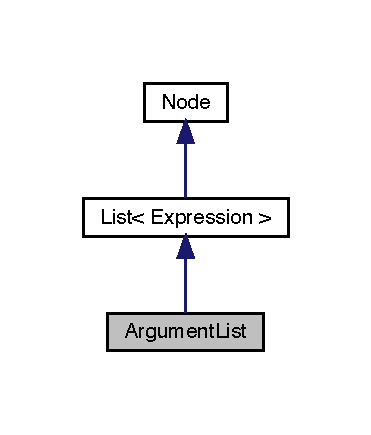
\includegraphics[width=178pt]{struct_argument_list__inherit__graph}
\end{center}
\end{figure}


Collaboration diagram for Argument\+List\+:\nopagebreak
\begin{figure}[H]
\begin{center}
\leavevmode
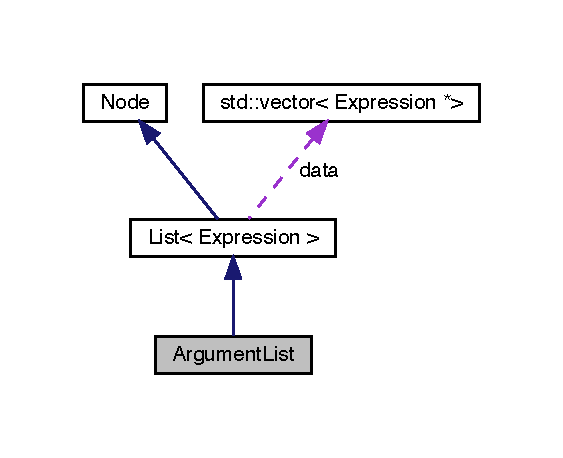
\includegraphics[width=270pt]{struct_argument_list__coll__graph}
\end{center}
\end{figure}
\subsection*{Public Member Functions}
\begin{DoxyCompactItemize}
\item 
{\footnotesize template$<$typename... Args$>$ }\\\hyperlink{struct_argument_list_a7df7f5009c8fc56cede100d66e45cb93}{Argument\+List} (Args \&\&... args)
\item 
void \hyperlink{struct_argument_list_af99815001d6a741b4a9fb0330971a7dc}{accept} (\hyperlink{struct_visitor}{Visitor} \&visitor) const override
\item 
const char $\ast$ \hyperlink{struct_argument_list_a40d37153eb093deadf7045b1ad5ae1fa}{type} () const override
\end{DoxyCompactItemize}
\subsection*{Additional Inherited Members}


\subsection{Constructor \& Destructor Documentation}
\mbox{\Hypertarget{struct_argument_list_a7df7f5009c8fc56cede100d66e45cb93}\label{struct_argument_list_a7df7f5009c8fc56cede100d66e45cb93}} 
\index{Argument\+List@{Argument\+List}!Argument\+List@{Argument\+List}}
\index{Argument\+List@{Argument\+List}!Argument\+List@{Argument\+List}}
\subsubsection{\texorpdfstring{Argument\+List()}{ArgumentList()}}
{\footnotesize\ttfamily template$<$typename... Args$>$ \\
Argument\+List\+::\+Argument\+List (\begin{DoxyParamCaption}\item[{Args \&\&...}]{args }\end{DoxyParamCaption})\hspace{0.3cm}{\ttfamily [inline]}}



\subsection{Member Function Documentation}
\mbox{\Hypertarget{struct_argument_list_af99815001d6a741b4a9fb0330971a7dc}\label{struct_argument_list_af99815001d6a741b4a9fb0330971a7dc}} 
\index{Argument\+List@{Argument\+List}!accept@{accept}}
\index{accept@{accept}!Argument\+List@{Argument\+List}}
\subsubsection{\texorpdfstring{accept()}{accept()}}
{\footnotesize\ttfamily void Argument\+List\+::accept (\begin{DoxyParamCaption}\item[{\hyperlink{struct_visitor}{Visitor} \&}]{visitor }\end{DoxyParamCaption}) const\hspace{0.3cm}{\ttfamily [inline]}, {\ttfamily [override]}, {\ttfamily [virtual]}}



Implements \hyperlink{struct_node_a10bd7af968140bbf5fa461298a969c71}{Node}.

\mbox{\Hypertarget{struct_argument_list_a40d37153eb093deadf7045b1ad5ae1fa}\label{struct_argument_list_a40d37153eb093deadf7045b1ad5ae1fa}} 
\index{Argument\+List@{Argument\+List}!type@{type}}
\index{type@{type}!Argument\+List@{Argument\+List}}
\subsubsection{\texorpdfstring{type()}{type()}}
{\footnotesize\ttfamily const char$\ast$ Argument\+List\+::type (\begin{DoxyParamCaption}{ }\end{DoxyParamCaption}) const\hspace{0.3cm}{\ttfamily [inline]}, {\ttfamily [override]}, {\ttfamily [virtual]}}



Implements \hyperlink{struct_node_a82f29420d0a38efcc370352528e94e9b}{Node}.



The documentation for this struct was generated from the following file\+:\begin{DoxyCompactItemize}
\item 
src/\hyperlink{ast_8h}{ast.\+h}\end{DoxyCompactItemize}

\hypertarget{struct_arguments}{}\section{Arguments Struct Reference}
\label{struct_arguments}\index{Arguments@{Arguments}}


{\ttfamily \#include $<$ast.\+h$>$}



Collaboration diagram for Arguments\+:\nopagebreak
\begin{figure}[H]
\begin{center}
\leavevmode
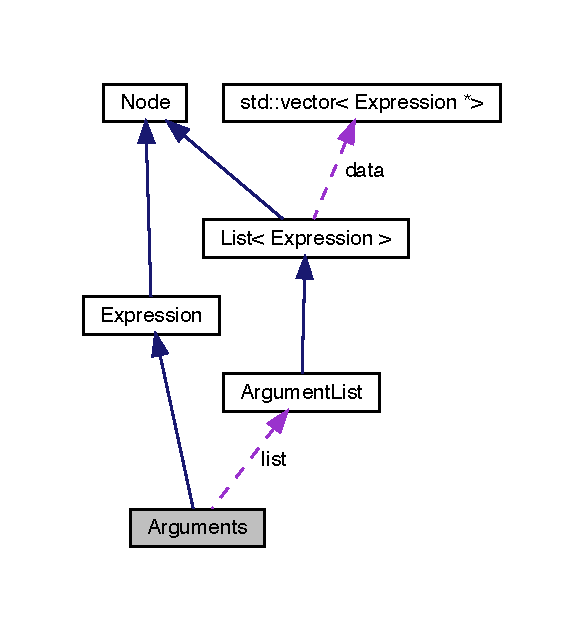
\includegraphics[width=209pt]{struct_arguments__coll__graph}
\end{center}
\end{figure}
\subsection*{Public Attributes}
\begin{DoxyCompactItemize}
\item 
\hyperlink{ast_8h_a31fcc1ca3d32657e8eb6f1433e97d2c9}{Argument\+List} \hyperlink{struct_arguments_aabd86069d52c369cfb9a9041fc991a83}{list}
\end{DoxyCompactItemize}


\subsection{Member Data Documentation}
\mbox{\Hypertarget{struct_arguments_aabd86069d52c369cfb9a9041fc991a83}\label{struct_arguments_aabd86069d52c369cfb9a9041fc991a83}} 
\index{Arguments@{Arguments}!list@{list}}
\index{list@{list}!Arguments@{Arguments}}
\subsubsection{\texorpdfstring{list}{list}}
{\footnotesize\ttfamily \hyperlink{ast_8h_a31fcc1ca3d32657e8eb6f1433e97d2c9}{Argument\+List} Arguments\+::list}



The documentation for this struct was generated from the following file\+:\begin{DoxyCompactItemize}
\item 
src/\hyperlink{ast_8h}{ast.\+h}\end{DoxyCompactItemize}

\hypertarget{struct_array_expression}{}\section{Array\+Expression Struct Reference}
\label{struct_array_expression}\index{Array\+Expression@{Array\+Expression}}


{\ttfamily \#include $<$ast.\+h$>$}



Inheritance diagram for Array\+Expression\+:
\nopagebreak
\begin{figure}[H]
\begin{center}
\leavevmode
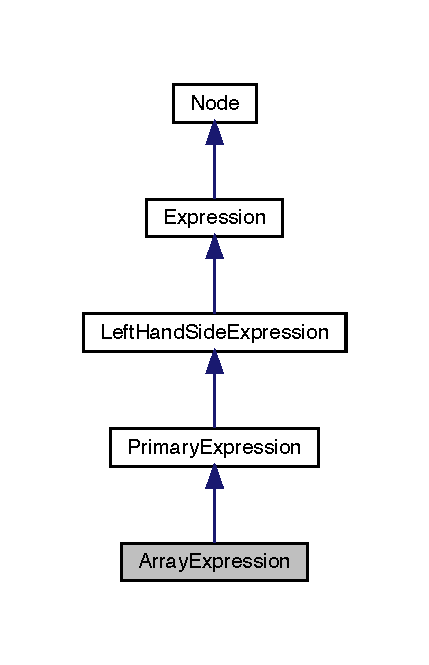
\includegraphics[width=206pt]{struct_array_expression__inherit__graph}
\end{center}
\end{figure}


Collaboration diagram for Array\+Expression\+:
\nopagebreak
\begin{figure}[H]
\begin{center}
\leavevmode
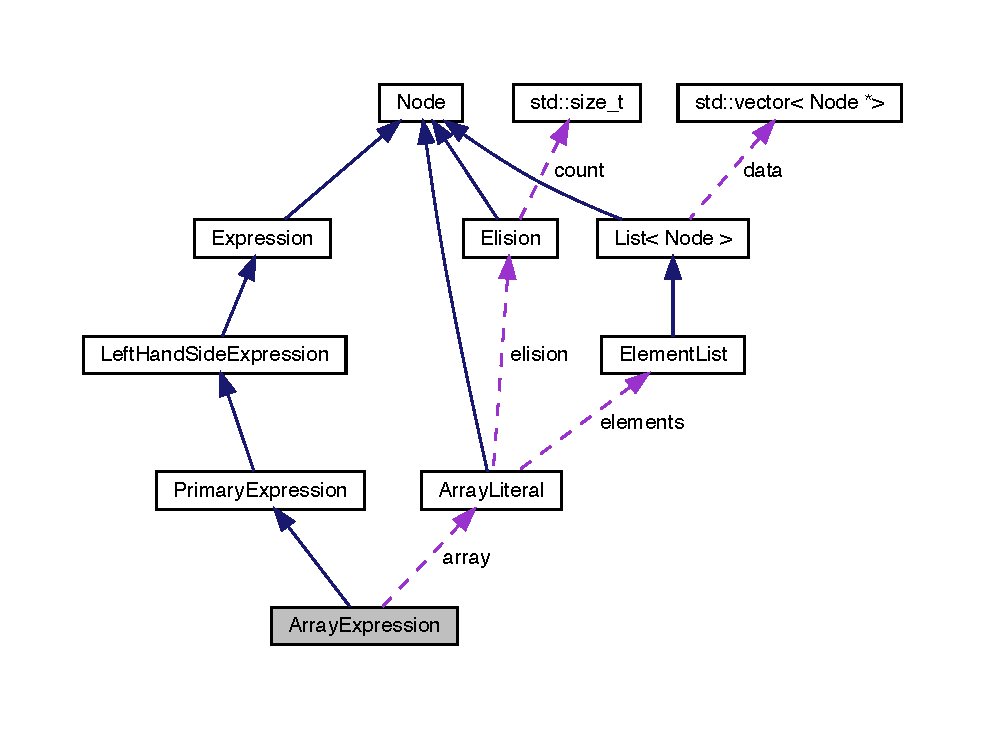
\includegraphics[width=350pt]{struct_array_expression__coll__graph}
\end{center}
\end{figure}
\subsection*{Public Member Functions}
\begin{DoxyCompactItemize}
\item 
\hyperlink{struct_array_expression_ae28e87942dea36d36f3e17460deebbad}{Array\+Expression} (\hyperlink{struct_array_literal}{Array\+Literal} $\ast$\hyperlink{struct_array_expression_a5eaa8dd89911611323de0d6f8221ac1d}{array})
\item 
void \hyperlink{struct_array_expression_a6f1d854ef3cfe2731aee50a45c774b5d}{accept} (\hyperlink{struct_visitor}{Visitor} \&visitor) const override
\item 
const char $\ast$ \hyperlink{struct_array_expression_ad0e148cb5a9de93a554e756cde23103e}{type} () const override
\end{DoxyCompactItemize}
\subsection*{Public Attributes}
\begin{DoxyCompactItemize}
\item 
\hyperlink{struct_array_literal}{Array\+Literal} $\ast$ \hyperlink{struct_array_expression_a5eaa8dd89911611323de0d6f8221ac1d}{array}
\end{DoxyCompactItemize}


\subsection{Constructor \& Destructor Documentation}
\mbox{\Hypertarget{struct_array_expression_ae28e87942dea36d36f3e17460deebbad}\label{struct_array_expression_ae28e87942dea36d36f3e17460deebbad}} 
\index{Array\+Expression@{Array\+Expression}!Array\+Expression@{Array\+Expression}}
\index{Array\+Expression@{Array\+Expression}!Array\+Expression@{Array\+Expression}}
\subsubsection{\texorpdfstring{Array\+Expression()}{ArrayExpression()}}
{\footnotesize\ttfamily Array\+Expression\+::\+Array\+Expression (\begin{DoxyParamCaption}\item[{\hyperlink{struct_array_literal}{Array\+Literal} $\ast$}]{array }\end{DoxyParamCaption})\hspace{0.3cm}{\ttfamily [inline]}}



\subsection{Member Function Documentation}
\mbox{\Hypertarget{struct_array_expression_a6f1d854ef3cfe2731aee50a45c774b5d}\label{struct_array_expression_a6f1d854ef3cfe2731aee50a45c774b5d}} 
\index{Array\+Expression@{Array\+Expression}!accept@{accept}}
\index{accept@{accept}!Array\+Expression@{Array\+Expression}}
\subsubsection{\texorpdfstring{accept()}{accept()}}
{\footnotesize\ttfamily void Array\+Expression\+::accept (\begin{DoxyParamCaption}\item[{\hyperlink{struct_visitor}{Visitor} \&}]{visitor }\end{DoxyParamCaption}) const\hspace{0.3cm}{\ttfamily [inline]}, {\ttfamily [override]}, {\ttfamily [virtual]}}



Implements \hyperlink{struct_node_a10bd7af968140bbf5fa461298a969c71}{Node}.

\mbox{\Hypertarget{struct_array_expression_ad0e148cb5a9de93a554e756cde23103e}\label{struct_array_expression_ad0e148cb5a9de93a554e756cde23103e}} 
\index{Array\+Expression@{Array\+Expression}!type@{type}}
\index{type@{type}!Array\+Expression@{Array\+Expression}}
\subsubsection{\texorpdfstring{type()}{type()}}
{\footnotesize\ttfamily const char$\ast$ Array\+Expression\+::type (\begin{DoxyParamCaption}{ }\end{DoxyParamCaption}) const\hspace{0.3cm}{\ttfamily [inline]}, {\ttfamily [override]}, {\ttfamily [virtual]}}



Implements \hyperlink{struct_node_a82f29420d0a38efcc370352528e94e9b}{Node}.



\subsection{Member Data Documentation}
\mbox{\Hypertarget{struct_array_expression_a5eaa8dd89911611323de0d6f8221ac1d}\label{struct_array_expression_a5eaa8dd89911611323de0d6f8221ac1d}} 
\index{Array\+Expression@{Array\+Expression}!array@{array}}
\index{array@{array}!Array\+Expression@{Array\+Expression}}
\subsubsection{\texorpdfstring{array}{array}}
{\footnotesize\ttfamily \hyperlink{struct_array_literal}{Array\+Literal}$\ast$ Array\+Expression\+::array}



The documentation for this struct was generated from the following file\+:\begin{DoxyCompactItemize}
\item 
src/\hyperlink{ast_8h}{ast.\+h}\end{DoxyCompactItemize}

\hypertarget{struct_array_literal}{}\section{Array\+Literal Struct Reference}
\label{struct_array_literal}\index{Array\+Literal@{Array\+Literal}}


{\ttfamily \#include $<$ast.\+h$>$}



Inheritance diagram for Array\+Literal\+:\nopagebreak
\begin{figure}[H]
\begin{center}
\leavevmode
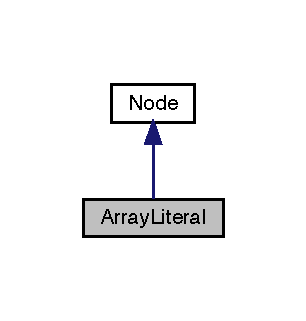
\includegraphics[width=147pt]{struct_array_literal__inherit__graph}
\end{center}
\end{figure}


Collaboration diagram for Array\+Literal\+:\nopagebreak
\begin{figure}[H]
\begin{center}
\leavevmode
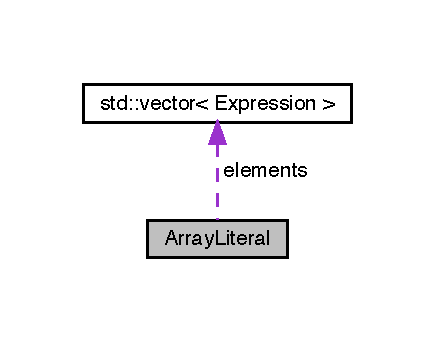
\includegraphics[width=324pt]{struct_array_literal__coll__graph}
\end{center}
\end{figure}
\subsection*{Public Member Functions}
\begin{DoxyCompactItemize}
\item 
\hyperlink{struct_array_literal_a1df7283ca804e7c1147f5024e2e0408d}{Array\+Literal} (\hyperlink{struct_element_list}{Element\+List} $\ast$\hyperlink{struct_array_literal_ae4c3df364c3994cb8916d73a50f1f92f}{elements}=nullptr, \hyperlink{struct_elision}{Elision} $\ast$\hyperlink{struct_array_literal_a08fa9ad6e83376bb2a70d22df9cf2c8a}{elision}=nullptr)
\item 
void \hyperlink{struct_array_literal_ab3ba06d627e0fe714aafb9fc843c83e8}{accept} (\hyperlink{struct_visitor}{Visitor} \&visitor) const override
\item 
const char $\ast$ \hyperlink{struct_array_literal_a24964c1f68d796d071b830b605046f51}{type} () const override
\end{DoxyCompactItemize}
\subsection*{Public Attributes}
\begin{DoxyCompactItemize}
\item 
\hyperlink{struct_element_list}{Element\+List} $\ast$ \hyperlink{struct_array_literal_ae4c3df364c3994cb8916d73a50f1f92f}{elements}
\item 
\hyperlink{struct_elision}{Elision} $\ast$ \hyperlink{struct_array_literal_a08fa9ad6e83376bb2a70d22df9cf2c8a}{elision}
\end{DoxyCompactItemize}


\subsection{Constructor \& Destructor Documentation}
\mbox{\Hypertarget{struct_array_literal_a1df7283ca804e7c1147f5024e2e0408d}\label{struct_array_literal_a1df7283ca804e7c1147f5024e2e0408d}} 
\index{Array\+Literal@{Array\+Literal}!Array\+Literal@{Array\+Literal}}
\index{Array\+Literal@{Array\+Literal}!Array\+Literal@{Array\+Literal}}
\subsubsection{\texorpdfstring{Array\+Literal()}{ArrayLiteral()}}
{\footnotesize\ttfamily Array\+Literal\+::\+Array\+Literal (\begin{DoxyParamCaption}\item[{\hyperlink{struct_element_list}{Element\+List} $\ast$}]{elements = {\ttfamily nullptr},  }\item[{\hyperlink{struct_elision}{Elision} $\ast$}]{elision = {\ttfamily nullptr} }\end{DoxyParamCaption})\hspace{0.3cm}{\ttfamily [inline]}}



\subsection{Member Function Documentation}
\mbox{\Hypertarget{struct_array_literal_ab3ba06d627e0fe714aafb9fc843c83e8}\label{struct_array_literal_ab3ba06d627e0fe714aafb9fc843c83e8}} 
\index{Array\+Literal@{Array\+Literal}!accept@{accept}}
\index{accept@{accept}!Array\+Literal@{Array\+Literal}}
\subsubsection{\texorpdfstring{accept()}{accept()}}
{\footnotesize\ttfamily void Array\+Literal\+::accept (\begin{DoxyParamCaption}\item[{\hyperlink{struct_visitor}{Visitor} \&}]{visitor }\end{DoxyParamCaption}) const\hspace{0.3cm}{\ttfamily [inline]}, {\ttfamily [override]}, {\ttfamily [virtual]}}



Implements \hyperlink{struct_node_a10bd7af968140bbf5fa461298a969c71}{Node}.

\mbox{\Hypertarget{struct_array_literal_a24964c1f68d796d071b830b605046f51}\label{struct_array_literal_a24964c1f68d796d071b830b605046f51}} 
\index{Array\+Literal@{Array\+Literal}!type@{type}}
\index{type@{type}!Array\+Literal@{Array\+Literal}}
\subsubsection{\texorpdfstring{type()}{type()}}
{\footnotesize\ttfamily const char$\ast$ Array\+Literal\+::type (\begin{DoxyParamCaption}{ }\end{DoxyParamCaption}) const\hspace{0.3cm}{\ttfamily [inline]}, {\ttfamily [override]}, {\ttfamily [virtual]}}



Implements \hyperlink{struct_node_a82f29420d0a38efcc370352528e94e9b}{Node}.



\subsection{Member Data Documentation}
\mbox{\Hypertarget{struct_array_literal_ae4c3df364c3994cb8916d73a50f1f92f}\label{struct_array_literal_ae4c3df364c3994cb8916d73a50f1f92f}} 
\index{Array\+Literal@{Array\+Literal}!elements@{elements}}
\index{elements@{elements}!Array\+Literal@{Array\+Literal}}
\subsubsection{\texorpdfstring{elements}{elements}}
{\footnotesize\ttfamily \hyperlink{struct_element_list}{Element\+List}$\ast$ Array\+Literal\+::elements}

\mbox{\Hypertarget{struct_array_literal_a08fa9ad6e83376bb2a70d22df9cf2c8a}\label{struct_array_literal_a08fa9ad6e83376bb2a70d22df9cf2c8a}} 
\index{Array\+Literal@{Array\+Literal}!elision@{elision}}
\index{elision@{elision}!Array\+Literal@{Array\+Literal}}
\subsubsection{\texorpdfstring{elision}{elision}}
{\footnotesize\ttfamily \hyperlink{struct_elision}{Elision}$\ast$ Array\+Literal\+::elision}



The documentation for this struct was generated from the following file\+:\begin{DoxyCompactItemize}
\item 
src/\hyperlink{ast_8h}{ast.\+h}\end{DoxyCompactItemize}

\hypertarget{struct_assignment_expression}{}\section{Assignment\+Expression Struct Reference}
\label{struct_assignment_expression}\index{Assignment\+Expression@{Assignment\+Expression}}


{\ttfamily \#include $<$ast.\+h$>$}



Inheritance diagram for Assignment\+Expression\+:
\nopagebreak
\begin{figure}[H]
\begin{center}
\leavevmode
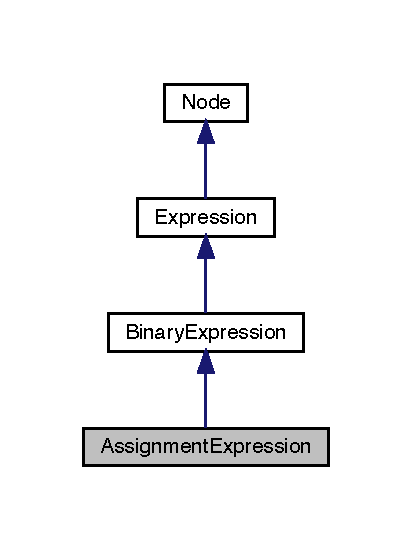
\includegraphics[width=198pt]{struct_assignment_expression__inherit__graph}
\end{center}
\end{figure}


Collaboration diagram for Assignment\+Expression\+:
\nopagebreak
\begin{figure}[H]
\begin{center}
\leavevmode
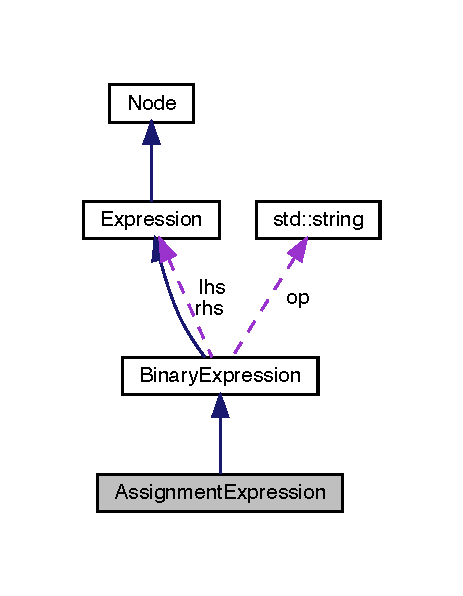
\includegraphics[width=222pt]{struct_assignment_expression__coll__graph}
\end{center}
\end{figure}
\subsection*{Public Member Functions}
\begin{DoxyCompactItemize}
\item 
\hyperlink{struct_assignment_expression_a52c4ebecbb914085110db6fdef413ae6}{Assignment\+Expression} (\textbf{ std\+::string} \hyperlink{struct_binary_expression_a4c33b66e2ffc0a5ede2cdd190bf4bd75}{op}, \hyperlink{struct_expression}{Expression} $\ast$\hyperlink{struct_binary_expression_ae689284a646929c99e634e75f50cb32c}{lhs}=nullptr, \hyperlink{struct_expression}{Expression} $\ast$\hyperlink{struct_binary_expression_ad569ae3b07f428257b0e7a96746ceb32}{rhs}=nullptr)
\item 
void \hyperlink{struct_assignment_expression_ac3d1a00abf176502782937938f629a9f}{accept} (\hyperlink{struct_visitor}{Visitor} \&visitor) const override
\item 
const char $\ast$ \hyperlink{struct_assignment_expression_a9c5da03eec8d7c10f1127ec5029de263}{type} () const override
\end{DoxyCompactItemize}
\subsection*{Additional Inherited Members}


\subsection{Constructor \& Destructor Documentation}
\mbox{\Hypertarget{struct_assignment_expression_a52c4ebecbb914085110db6fdef413ae6}\label{struct_assignment_expression_a52c4ebecbb914085110db6fdef413ae6}} 
\index{Assignment\+Expression@{Assignment\+Expression}!Assignment\+Expression@{Assignment\+Expression}}
\index{Assignment\+Expression@{Assignment\+Expression}!Assignment\+Expression@{Assignment\+Expression}}
\subsubsection{\texorpdfstring{Assignment\+Expression()}{AssignmentExpression()}}
{\footnotesize\ttfamily Assignment\+Expression\+::\+Assignment\+Expression (\begin{DoxyParamCaption}\item[{\textbf{ std\+::string}}]{op,  }\item[{\hyperlink{struct_expression}{Expression} $\ast$}]{lhs = {\ttfamily nullptr},  }\item[{\hyperlink{struct_expression}{Expression} $\ast$}]{rhs = {\ttfamily nullptr} }\end{DoxyParamCaption})\hspace{0.3cm}{\ttfamily [inline]}}



\subsection{Member Function Documentation}
\mbox{\Hypertarget{struct_assignment_expression_ac3d1a00abf176502782937938f629a9f}\label{struct_assignment_expression_ac3d1a00abf176502782937938f629a9f}} 
\index{Assignment\+Expression@{Assignment\+Expression}!accept@{accept}}
\index{accept@{accept}!Assignment\+Expression@{Assignment\+Expression}}
\subsubsection{\texorpdfstring{accept()}{accept()}}
{\footnotesize\ttfamily void Assignment\+Expression\+::accept (\begin{DoxyParamCaption}\item[{\hyperlink{struct_visitor}{Visitor} \&}]{visitor }\end{DoxyParamCaption}) const\hspace{0.3cm}{\ttfamily [inline]}, {\ttfamily [override]}, {\ttfamily [virtual]}}



Reimplemented from \hyperlink{struct_binary_expression_af8318bd8b21b4bbca064e8a6086a10a0}{Binary\+Expression}.

\mbox{\Hypertarget{struct_assignment_expression_a9c5da03eec8d7c10f1127ec5029de263}\label{struct_assignment_expression_a9c5da03eec8d7c10f1127ec5029de263}} 
\index{Assignment\+Expression@{Assignment\+Expression}!type@{type}}
\index{type@{type}!Assignment\+Expression@{Assignment\+Expression}}
\subsubsection{\texorpdfstring{type()}{type()}}
{\footnotesize\ttfamily const char$\ast$ Assignment\+Expression\+::type (\begin{DoxyParamCaption}{ }\end{DoxyParamCaption}) const\hspace{0.3cm}{\ttfamily [inline]}, {\ttfamily [override]}, {\ttfamily [virtual]}}



Reimplemented from \hyperlink{struct_binary_expression_a9ab583e823bac39ed8fd8eb34747ac9f}{Binary\+Expression}.



The documentation for this struct was generated from the following file\+:\begin{DoxyCompactItemize}
\item 
src/\hyperlink{ast_8h}{ast.\+h}\end{DoxyCompactItemize}

\hypertarget{class_basic_lexer}{}\section{Basic\+Lexer$<$ T $>$ Class Template Reference}
\label{class_basic_lexer}\index{Basic\+Lexer$<$ T $>$@{Basic\+Lexer$<$ T $>$}}


{\ttfamily \#include $<$lexer.\+h$>$}



Inheritance diagram for Basic\+Lexer$<$ T $>$\+:\nopagebreak
\begin{figure}[H]
\begin{center}
\leavevmode
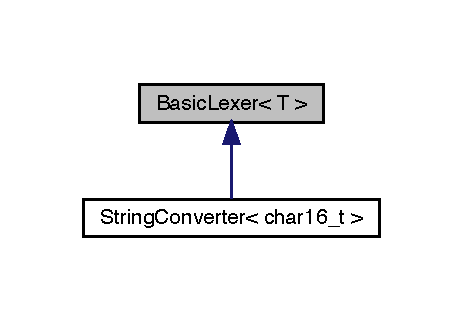
\includegraphics[width=222pt]{class_basic_lexer__inherit__graph}
\end{center}
\end{figure}
\subsection*{Public Member Functions}
\begin{DoxyCompactItemize}
\item 
\hyperlink{class_basic_lexer_abc267aed0ef7227486b932f13b2917f0}{Basic\+Lexer} ()
\item 
\hyperlink{class_basic_lexer_a58d2038fb47025d4e32c20750e713b43}{Basic\+Lexer} (\textbf{ std\+::initializer\+\_\+list}$<$ \hyperlink{class_token}{Token} $>$ \hyperlink{class_basic_lexer_ac20fdf19d5602c563b5cad2bae3ad803}{tokens})
\item 
\hyperlink{class_basic_lexer_a1fd5d2795464497ffbe2bf61c892d619}{Basic\+Lexer} (\textbf{ std\+::vector}$<$ \hyperlink{class_token}{Token} $>$ \hyperlink{class_basic_lexer_ac20fdf19d5602c563b5cad2bae3ad803}{tokens})
\item 
{\footnotesize template$<$typename It $>$ }\\\hyperlink{class_basic_lexer_a7b8cb3ec8ba1ef5567bd280800f891f8}{Basic\+Lexer} (It begin, It end)
\item 
\hyperlink{class_basic_lexer_aee8242905dd2c3541322900bdd05a7b7}{Basic\+Lexer} (const \textbf{ std\+::u16string} \&str)
\item 
\hyperlink{class_basic_lexer_ab486a96453887dc7f9efd08c518ae0b0}{Basic\+Lexer} (const \textbf{ std\+::string} \&str)
\item 
Tokens \hyperlink{class_basic_lexer_ac20fdf19d5602c563b5cad2bae3ad803}{tokens} () const
\end{DoxyCompactItemize}


\subsection{Constructor \& Destructor Documentation}
\mbox{\Hypertarget{class_basic_lexer_abc267aed0ef7227486b932f13b2917f0}\label{class_basic_lexer_abc267aed0ef7227486b932f13b2917f0}} 
\index{Basic\+Lexer@{Basic\+Lexer}!Basic\+Lexer@{Basic\+Lexer}}
\index{Basic\+Lexer@{Basic\+Lexer}!Basic\+Lexer@{Basic\+Lexer}}
\subsubsection{\texorpdfstring{Basic\+Lexer()}{BasicLexer()}\hspace{0.1cm}{\footnotesize\ttfamily [1/6]}}
{\footnotesize\ttfamily template$<$typename T$>$ \\
\hyperlink{class_basic_lexer}{Basic\+Lexer}$<$ T $>$\+::\hyperlink{class_basic_lexer}{Basic\+Lexer} (\begin{DoxyParamCaption}{ }\end{DoxyParamCaption})\hspace{0.3cm}{\ttfamily [inline]}}

\mbox{\Hypertarget{class_basic_lexer_a58d2038fb47025d4e32c20750e713b43}\label{class_basic_lexer_a58d2038fb47025d4e32c20750e713b43}} 
\index{Basic\+Lexer@{Basic\+Lexer}!Basic\+Lexer@{Basic\+Lexer}}
\index{Basic\+Lexer@{Basic\+Lexer}!Basic\+Lexer@{Basic\+Lexer}}
\subsubsection{\texorpdfstring{Basic\+Lexer()}{BasicLexer()}\hspace{0.1cm}{\footnotesize\ttfamily [2/6]}}
{\footnotesize\ttfamily template$<$typename T$>$ \\
\hyperlink{class_basic_lexer}{Basic\+Lexer}$<$ T $>$\+::\hyperlink{class_basic_lexer}{Basic\+Lexer} (\begin{DoxyParamCaption}\item[{\textbf{ std\+::initializer\+\_\+list}$<$ \hyperlink{class_token}{Token} $>$}]{tokens }\end{DoxyParamCaption})\hspace{0.3cm}{\ttfamily [inline]}}

\mbox{\Hypertarget{class_basic_lexer_a1fd5d2795464497ffbe2bf61c892d619}\label{class_basic_lexer_a1fd5d2795464497ffbe2bf61c892d619}} 
\index{Basic\+Lexer@{Basic\+Lexer}!Basic\+Lexer@{Basic\+Lexer}}
\index{Basic\+Lexer@{Basic\+Lexer}!Basic\+Lexer@{Basic\+Lexer}}
\subsubsection{\texorpdfstring{Basic\+Lexer()}{BasicLexer()}\hspace{0.1cm}{\footnotesize\ttfamily [3/6]}}
{\footnotesize\ttfamily template$<$typename T$>$ \\
\hyperlink{class_basic_lexer}{Basic\+Lexer}$<$ T $>$\+::\hyperlink{class_basic_lexer}{Basic\+Lexer} (\begin{DoxyParamCaption}\item[{\textbf{ std\+::vector}$<$ \hyperlink{class_token}{Token} $>$}]{tokens }\end{DoxyParamCaption})\hspace{0.3cm}{\ttfamily [inline]}}

\mbox{\Hypertarget{class_basic_lexer_a7b8cb3ec8ba1ef5567bd280800f891f8}\label{class_basic_lexer_a7b8cb3ec8ba1ef5567bd280800f891f8}} 
\index{Basic\+Lexer@{Basic\+Lexer}!Basic\+Lexer@{Basic\+Lexer}}
\index{Basic\+Lexer@{Basic\+Lexer}!Basic\+Lexer@{Basic\+Lexer}}
\subsubsection{\texorpdfstring{Basic\+Lexer()}{BasicLexer()}\hspace{0.1cm}{\footnotesize\ttfamily [4/6]}}
{\footnotesize\ttfamily template$<$typename T$>$ \\
template$<$typename It $>$ \\
\hyperlink{class_basic_lexer}{Basic\+Lexer}$<$ T $>$\+::\hyperlink{class_basic_lexer}{Basic\+Lexer} (\begin{DoxyParamCaption}\item[{It}]{begin,  }\item[{It}]{end }\end{DoxyParamCaption})\hspace{0.3cm}{\ttfamily [inline]}}

\mbox{\Hypertarget{class_basic_lexer_aee8242905dd2c3541322900bdd05a7b7}\label{class_basic_lexer_aee8242905dd2c3541322900bdd05a7b7}} 
\index{Basic\+Lexer@{Basic\+Lexer}!Basic\+Lexer@{Basic\+Lexer}}
\index{Basic\+Lexer@{Basic\+Lexer}!Basic\+Lexer@{Basic\+Lexer}}
\subsubsection{\texorpdfstring{Basic\+Lexer()}{BasicLexer()}\hspace{0.1cm}{\footnotesize\ttfamily [5/6]}}
{\footnotesize\ttfamily template$<$typename T$>$ \\
\hyperlink{class_basic_lexer}{Basic\+Lexer}$<$ T $>$\+::\hyperlink{class_basic_lexer}{Basic\+Lexer} (\begin{DoxyParamCaption}\item[{const \textbf{ std\+::u16string} \&}]{str }\end{DoxyParamCaption})\hspace{0.3cm}{\ttfamily [inline]}}

\mbox{\Hypertarget{class_basic_lexer_ab486a96453887dc7f9efd08c518ae0b0}\label{class_basic_lexer_ab486a96453887dc7f9efd08c518ae0b0}} 
\index{Basic\+Lexer@{Basic\+Lexer}!Basic\+Lexer@{Basic\+Lexer}}
\index{Basic\+Lexer@{Basic\+Lexer}!Basic\+Lexer@{Basic\+Lexer}}
\subsubsection{\texorpdfstring{Basic\+Lexer()}{BasicLexer()}\hspace{0.1cm}{\footnotesize\ttfamily [6/6]}}
{\footnotesize\ttfamily template$<$typename T$>$ \\
\hyperlink{class_basic_lexer}{Basic\+Lexer}$<$ T $>$\+::\hyperlink{class_basic_lexer}{Basic\+Lexer} (\begin{DoxyParamCaption}\item[{const \textbf{ std\+::string} \&}]{str }\end{DoxyParamCaption})\hspace{0.3cm}{\ttfamily [inline]}}



\subsection{Member Function Documentation}
\mbox{\Hypertarget{class_basic_lexer_ac20fdf19d5602c563b5cad2bae3ad803}\label{class_basic_lexer_ac20fdf19d5602c563b5cad2bae3ad803}} 
\index{Basic\+Lexer@{Basic\+Lexer}!tokens@{tokens}}
\index{tokens@{tokens}!Basic\+Lexer@{Basic\+Lexer}}
\subsubsection{\texorpdfstring{tokens()}{tokens()}}
{\footnotesize\ttfamily template$<$typename T$>$ \\
Tokens \hyperlink{class_basic_lexer}{Basic\+Lexer}$<$ T $>$\+::tokens (\begin{DoxyParamCaption}{ }\end{DoxyParamCaption}) const\hspace{0.3cm}{\ttfamily [inline]}}



The documentation for this class was generated from the following file\+:\begin{DoxyCompactItemize}
\item 
src/\hyperlink{lexer_8h}{lexer.\+h}\end{DoxyCompactItemize}

\hypertarget{struct_basic_visitor}{}\section{Basic\+Visitor Struct Reference}
\label{struct_basic_visitor}\index{Basic\+Visitor@{Basic\+Visitor}}


{\ttfamily \#include $<$basic\+\_\+visitor.\+h$>$}



Inheritance diagram for Basic\+Visitor\+:\nopagebreak
\begin{figure}[H]
\begin{center}
\leavevmode
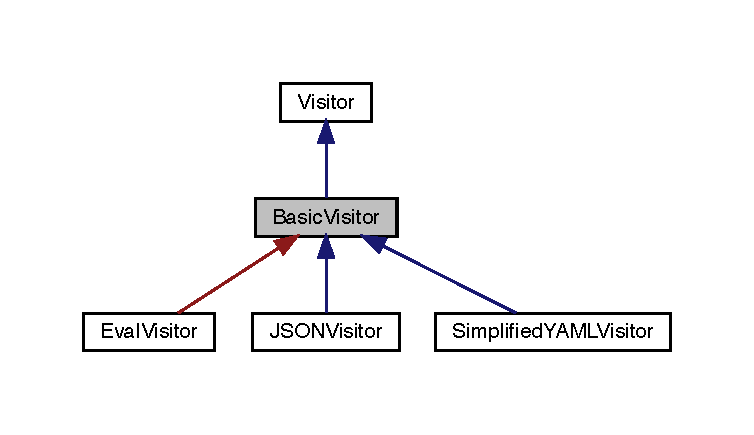
\includegraphics[width=350pt]{struct_basic_visitor__inherit__graph}
\end{center}
\end{figure}


Collaboration diagram for Basic\+Visitor\+:\nopagebreak
\begin{figure}[H]
\begin{center}
\leavevmode
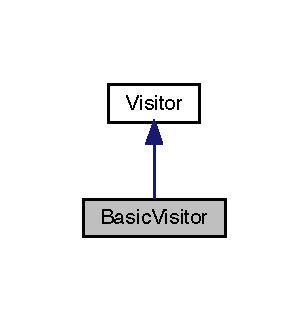
\includegraphics[width=148pt]{struct_basic_visitor__coll__graph}
\end{center}
\end{figure}
\subsection*{Public Member Functions}
\begin{DoxyCompactItemize}
\item 
{\footnotesize template$<$typename T $>$ }\\void \hyperlink{struct_basic_visitor_aef8aa82a7e5149b6153f097af8daa647}{apply\+\_\+impl} (const T $\ast$node)
\item 
{\footnotesize template$<$typename T $>$ }\\void \hyperlink{struct_basic_visitor_a128388a75069690c9c108ce87b69cde8}{apply\+\_\+impl} (const \textbf{ std\+::vector}$<$ T $>$ \&list)
\item 
{\footnotesize template$<$typename... Args$>$ }\\void \hyperlink{struct_basic_visitor_a85afee760b9e02733ed01ff56a96f09c}{apply} (Args \&\&... args)
\item 
void \hyperlink{struct_basic_visitor_a15fc407e84d51dad443c3b7e135302ae}{operator()} (const \hyperlink{struct_this}{This} \&) override
\item 
void \hyperlink{struct_basic_visitor_ac9ae9d17e262b8c71696d978be89af4d}{operator()} (const \hyperlink{struct_identifier}{Identifier} \&) override
\item 
void \hyperlink{struct_basic_visitor_afc1fe7c3d76c98c6d489d98c66d773de}{operator()} (const \hyperlink{struct_null_literal}{Null\+Literal} \&) override
\item 
void \hyperlink{struct_basic_visitor_a2971ac256de1c7b0206b44f888d9abd5}{operator()} (const \hyperlink{struct_boolean_literal}{Boolean\+Literal} \&) override
\item 
void \hyperlink{struct_basic_visitor_a177e744fc03783b7fbb83d3292a7c029}{operator()} (const \hyperlink{struct_numeric_literal}{Numeric\+Literal} \&) override
\item 
void \hyperlink{struct_basic_visitor_a1e22bd82234168dd70579eabe84574ad}{operator()} (const \hyperlink{struct_string_literal}{String\+Literal} \&) override
\item 
void \hyperlink{struct_basic_visitor_a40d181efc4db66a595baaee6e78c65db}{operator()} (const \hyperlink{struct_regular_expression_literal}{Regular\+Expression\+Literal} \&) override
\item 
void \hyperlink{struct_basic_visitor_a0f625d975e964cda064bbc0f12f97558}{operator()} (const \hyperlink{struct_array_literal}{Array\+Literal} \&node) override
\item 
void \hyperlink{struct_basic_visitor_a1f0d676e1575a8efa7fd7149ef9d93be}{operator()} (const \hyperlink{struct_object_literal}{Object\+Literal} \&node) override
\item 
void \hyperlink{struct_basic_visitor_aa3811d723e70227de815461380d861c9}{operator()} (const \hyperlink{struct_this_expression}{This\+Expression} \&) override
\item 
void \hyperlink{struct_basic_visitor_a453bc258129808d4e1e1efefcfa893a0}{operator()} (const \hyperlink{struct_identifier_expression}{Identifier\+Expression} \&node) override
\item 
void \hyperlink{struct_basic_visitor_af86e1dfc1fb346b3dd94a63b6017f4d4}{operator()} (const \hyperlink{struct_literal_expression}{Literal\+Expression} \&node) override
\item 
void \hyperlink{struct_basic_visitor_a1b0936671dd80c4e4ce029e41b216ba6}{operator()} (const \hyperlink{struct_array_expression}{Array\+Expression} \&node) override
\item 
void \hyperlink{struct_basic_visitor_a2bdc5b88714c947eb15d5530240c660c}{operator()} (const \hyperlink{struct_object_expression}{Object\+Expression} \&node) override
\item 
void \hyperlink{struct_basic_visitor_a74c4ab927dc2907784f886245a29296b}{operator()} (const \hyperlink{struct_member_expression}{Member\+Expression} \&node) override
\item 
void \hyperlink{struct_basic_visitor_ab73b6e87ae7344434aa833bd93f4480b}{operator()} (const \hyperlink{struct_new_expression}{New\+Expression} \&node) override
\item 
void \hyperlink{struct_basic_visitor_a455b2414d59a21bae802bd8b20544252}{operator()} (const \hyperlink{struct_call_expression}{Call\+Expression} \&node) override
\item 
void \hyperlink{struct_basic_visitor_ac7e33b8e36fa46d32e3cf517bf9de9bb}{operator()} (const \hyperlink{struct_postfix_expression}{Postfix\+Expression} \&node) override
\item 
void \hyperlink{struct_basic_visitor_a3ae4c9623d2f589f6f026833a7c1dd13}{operator()} (const \hyperlink{struct_unary_expression}{Unary\+Expression} \&node) override
\item 
void \hyperlink{struct_basic_visitor_a9433a6a9dcdd64f97ea1c392208a3305}{operator()} (const \hyperlink{struct_binary_expression}{Binary\+Expression} \&node) override
\item 
void \hyperlink{struct_basic_visitor_ab121f54f6337dc726745c65f47812d8d}{operator()} (const \hyperlink{struct_conditional_expression}{Conditional\+Expression} \&node) override
\item 
void \hyperlink{struct_basic_visitor_a8b5be95fdf83d05891a738923bace2be}{operator()} (const \hyperlink{struct_assignment_expression}{Assignment\+Expression} \&node) override
\item 
void \hyperlink{struct_basic_visitor_ae6e86620ac38764d055615b005b7a1d4}{operator()} (const \hyperlink{struct_function_expression}{Function\+Expression} \&node) override
\item 
void \hyperlink{struct_basic_visitor_a6ab713b4b992eb420c89a2326e351fd3}{operator()} (const \hyperlink{struct_block}{Block} \&node) override
\item 
void \hyperlink{struct_basic_visitor_afb110c94ddb7c8383f03541c76ff8bf7}{operator()} (const \hyperlink{struct_variable_statement}{Variable\+Statement} \&stmt) override
\item 
void \hyperlink{struct_basic_visitor_a99efd6097eb643d8738f1bb42f51f17e}{operator()} (const \hyperlink{struct_empty_statement}{Empty\+Statement} \&) override
\item 
void \hyperlink{struct_basic_visitor_a6c369f60a28dffd5149258e32a81cb6e}{operator()} (const \hyperlink{struct_expression_statement}{Expression\+Statement} \&stmt) override
\item 
void \hyperlink{struct_basic_visitor_a4d4e3621e47ea469c0e59d0b1c6c657b}{operator()} (const \hyperlink{struct_if_statement}{If\+Statement} \&stmt) override
\item 
void \hyperlink{struct_basic_visitor_a51de918d2508db22dba21233582f670e}{operator()} (const \hyperlink{struct_do_while_statement}{Do\+While\+Statement} \&) override
\item 
void \hyperlink{struct_basic_visitor_a0a7f4e29df8d0725070caa8560d4c4b5}{operator()} (const \hyperlink{struct_while_statement}{While\+Statement} \&) override
\item 
void \hyperlink{struct_basic_visitor_a62043123e2fb7e0c22229b0e5bb7dcc8}{operator()} (const \hyperlink{struct_for_statement}{For\+Statement} \&) override
\item 
void \hyperlink{struct_basic_visitor_abfa9eb036c3927634be4aef270579672}{operator()} (const \hyperlink{struct_for_in_statement}{For\+In\+Statement} \&) override
\item 
void \hyperlink{struct_basic_visitor_a5614facf759b3aa15b518df911cd9a6c}{operator()} (const \hyperlink{struct_continue_statement}{Continue\+Statement} \&stmt) override
\item 
void \hyperlink{struct_basic_visitor_ae0ecf9dc46dc7654488a1b2002dceb25}{operator()} (const \hyperlink{struct_break_statement}{Break\+Statement} \&stmt) override
\item 
void \hyperlink{struct_basic_visitor_ac7a0c630d96799333d3d32c8ca465f51}{operator()} (const \hyperlink{struct_return_statement}{Return\+Statement} \&stmt) override
\item 
void \hyperlink{struct_basic_visitor_a3dafb609d4df2fa786f7fe4fb25f1b9d}{operator()} (const \hyperlink{struct_with_statement}{With\+Statement} \&stmt) override
\item 
void \hyperlink{struct_basic_visitor_ae53f4199cddb021c0f30f898796942c4}{operator()} (const \hyperlink{struct_labelled_statement}{Labelled\+Statement} \&stmt) override
\item 
void \hyperlink{struct_basic_visitor_af97609b1ab2068d18ea5e94240819ccb}{operator()} (const \hyperlink{struct_switch_statement}{Switch\+Statement} \&stmt) override
\item 
void \hyperlink{struct_basic_visitor_a19c4ebe7b4d6d1cbddc354cf8e8267e4}{operator()} (const \hyperlink{struct_throw_statement}{Throw\+Statement} \&stmt) override
\item 
void \hyperlink{struct_basic_visitor_a2b4e8d7c1f46d71adbc8bf2f4b597fcc}{operator()} (const \hyperlink{struct_try_statement}{Try\+Statement} \&stmt) override
\item 
void \hyperlink{struct_basic_visitor_a193c296097cb56beab2cc74165668df8}{operator()} (const \hyperlink{struct_debugger_statement}{Debugger\+Statement} \&) override
\item 
void \hyperlink{struct_basic_visitor_ae3d4b26dfc7eaae787a33d9e1e73bc2e}{operator()} (const \hyperlink{struct_case_clause}{Case\+Clause} \&node) override
\item 
void \hyperlink{struct_basic_visitor_ae0235e556d05ba170398dcd7f0c25cb1}{operator()} (const \hyperlink{struct_default_clause}{Default\+Clause} \&node) override
\item 
void \hyperlink{struct_basic_visitor_a2871985a62b51f8f5212a5a65e47b7b8}{operator()} (const \hyperlink{struct_function_declaration}{Function\+Declaration} \&decl) override
\item 
void \hyperlink{struct_basic_visitor_ac9435a48d44ce32bd726cbf46bcc9032}{operator()} (const \hyperlink{struct_function_body}{Function\+Body} \&node) override
\item 
void \hyperlink{struct_basic_visitor_a0405c0df4a21c4735feaa98f5cd0cfa9}{operator()} (const \hyperlink{struct_variable_declaration}{Variable\+Declaration} \&decl) override
\item 
void \hyperlink{struct_basic_visitor_af64d7b88cbffe3d0717e9607704f56da}{operator()} (const \hyperlink{struct_elision}{Elision} \&) override
\item 
void \hyperlink{struct_basic_visitor_a4e82e722dc7c0cc04b1a39e0961b29f6}{operator()} (const \hyperlink{struct_property_name}{Property\+Name} \&) override
\item 
void \hyperlink{struct_basic_visitor_a3a868dc82a76118467f3a1ae4b1c92cd}{operator()} (const \hyperlink{struct_property_assignment}{Property\+Assignment} \&node) override
\item 
void \hyperlink{struct_basic_visitor_a8fecced7470cc28d2294c93e7df7ac1d}{operator()} (const \hyperlink{struct_arguments}{Arguments} \&node) override
\item 
void \hyperlink{struct_basic_visitor_adeaf13cc53c36c871d89d6f42a1ec8db}{operator()} (const \hyperlink{struct_program}{Program} \&node) override
\item 
void \hyperlink{struct_basic_visitor_a365071938626ac065ac413ba0e6d382f}{operator()} (const \hyperlink{struct_program_declaration}{Program\+Declaration} \&decl) override
\item 
void \hyperlink{struct_basic_visitor_ae04e6bd948d2f85acaff8744ad6ab0d7}{operator()} (const \hyperlink{struct_element_list}{Element\+List} \&list) override
\item 
void \hyperlink{struct_basic_visitor_a1cae5b2aa57d5214a6e89f6368ae5be1}{operator()} (const \hyperlink{struct_property_name_and_value_list}{Property\+Name\+And\+Value\+List} \&list) override
\item 
void \hyperlink{struct_basic_visitor_a3ebaf2b9a8a274df6d9960f1d6d8b6a6}{operator()} (const \hyperlink{struct_argument_list}{Argument\+List} \&list) override
\item 
void \hyperlink{struct_basic_visitor_aa04dfa4159f7711dcfd3d85ffab8ae88}{operator()} (const \hyperlink{struct_variable_declaration_list}{Variable\+Declaration\+List} \&list) override
\item 
void \hyperlink{struct_basic_visitor_a253a7061c246597f81f1122988704345}{operator()} (const \hyperlink{struct_statement_list}{Statement\+List} \&list) override
\item 
void \hyperlink{struct_basic_visitor_af108c842c7b483b2cb544dd77b171486}{operator()} (const \hyperlink{struct_case_block}{Case\+Block} \&list) override
\item 
void \hyperlink{struct_basic_visitor_a4cb8f522aa48db2270e3af61ee7b3370}{operator()} (const \hyperlink{struct_source_elements}{Source\+Elements} \&list) override
\item 
void \hyperlink{struct_basic_visitor_a3ce54960164c84e8d61c4c710362d6e3}{operator()} (const \hyperlink{struct_formal_parameter_list}{Formal\+Parameter\+List} \&list) override
\end{DoxyCompactItemize}


\subsection{Member Function Documentation}
\mbox{\Hypertarget{struct_basic_visitor_a85afee760b9e02733ed01ff56a96f09c}\label{struct_basic_visitor_a85afee760b9e02733ed01ff56a96f09c}} 
\index{Basic\+Visitor@{Basic\+Visitor}!apply@{apply}}
\index{apply@{apply}!Basic\+Visitor@{Basic\+Visitor}}
\subsubsection{\texorpdfstring{apply()}{apply()}}
{\footnotesize\ttfamily template$<$typename... Args$>$ \\
void Basic\+Visitor\+::apply (\begin{DoxyParamCaption}\item[{Args \&\&...}]{args }\end{DoxyParamCaption})\hspace{0.3cm}{\ttfamily [inline]}}

\mbox{\Hypertarget{struct_basic_visitor_aef8aa82a7e5149b6153f097af8daa647}\label{struct_basic_visitor_aef8aa82a7e5149b6153f097af8daa647}} 
\index{Basic\+Visitor@{Basic\+Visitor}!apply\+\_\+impl@{apply\+\_\+impl}}
\index{apply\+\_\+impl@{apply\+\_\+impl}!Basic\+Visitor@{Basic\+Visitor}}
\subsubsection{\texorpdfstring{apply\+\_\+impl()}{apply\_impl()}\hspace{0.1cm}{\footnotesize\ttfamily [1/2]}}
{\footnotesize\ttfamily template$<$typename T $>$ \\
void Basic\+Visitor\+::apply\+\_\+impl (\begin{DoxyParamCaption}\item[{const T $\ast$}]{node }\end{DoxyParamCaption})\hspace{0.3cm}{\ttfamily [inline]}}

\mbox{\Hypertarget{struct_basic_visitor_a128388a75069690c9c108ce87b69cde8}\label{struct_basic_visitor_a128388a75069690c9c108ce87b69cde8}} 
\index{Basic\+Visitor@{Basic\+Visitor}!apply\+\_\+impl@{apply\+\_\+impl}}
\index{apply\+\_\+impl@{apply\+\_\+impl}!Basic\+Visitor@{Basic\+Visitor}}
\subsubsection{\texorpdfstring{apply\+\_\+impl()}{apply\_impl()}\hspace{0.1cm}{\footnotesize\ttfamily [2/2]}}
{\footnotesize\ttfamily template$<$typename T $>$ \\
void Basic\+Visitor\+::apply\+\_\+impl (\begin{DoxyParamCaption}\item[{const \textbf{ std\+::vector}$<$ T $>$ \&}]{list }\end{DoxyParamCaption})\hspace{0.3cm}{\ttfamily [inline]}}

\mbox{\Hypertarget{struct_basic_visitor_a15fc407e84d51dad443c3b7e135302ae}\label{struct_basic_visitor_a15fc407e84d51dad443c3b7e135302ae}} 
\index{Basic\+Visitor@{Basic\+Visitor}!operator()@{operator()}}
\index{operator()@{operator()}!Basic\+Visitor@{Basic\+Visitor}}
\subsubsection{\texorpdfstring{operator()()}{operator()()}\hspace{0.1cm}{\footnotesize\ttfamily [1/60]}}
{\footnotesize\ttfamily void Basic\+Visitor\+::operator() (\begin{DoxyParamCaption}\item[{const \hyperlink{struct_this}{This} \&}]{ }\end{DoxyParamCaption})\hspace{0.3cm}{\ttfamily [inline]}, {\ttfamily [override]}, {\ttfamily [virtual]}}



Implements \hyperlink{struct_visitor_a7a043c9da4e7f8233db48afb82dbc7bc}{Visitor}.

\mbox{\Hypertarget{struct_basic_visitor_ac9ae9d17e262b8c71696d978be89af4d}\label{struct_basic_visitor_ac9ae9d17e262b8c71696d978be89af4d}} 
\index{Basic\+Visitor@{Basic\+Visitor}!operator()@{operator()}}
\index{operator()@{operator()}!Basic\+Visitor@{Basic\+Visitor}}
\subsubsection{\texorpdfstring{operator()()}{operator()()}\hspace{0.1cm}{\footnotesize\ttfamily [2/60]}}
{\footnotesize\ttfamily void Basic\+Visitor\+::operator() (\begin{DoxyParamCaption}\item[{const \hyperlink{struct_identifier}{Identifier} \&}]{ }\end{DoxyParamCaption})\hspace{0.3cm}{\ttfamily [inline]}, {\ttfamily [override]}, {\ttfamily [virtual]}}



Implements \hyperlink{struct_visitor_a2d09687aa24b1b618c6205f8413c2dd3}{Visitor}.

\mbox{\Hypertarget{struct_basic_visitor_afc1fe7c3d76c98c6d489d98c66d773de}\label{struct_basic_visitor_afc1fe7c3d76c98c6d489d98c66d773de}} 
\index{Basic\+Visitor@{Basic\+Visitor}!operator()@{operator()}}
\index{operator()@{operator()}!Basic\+Visitor@{Basic\+Visitor}}
\subsubsection{\texorpdfstring{operator()()}{operator()()}\hspace{0.1cm}{\footnotesize\ttfamily [3/60]}}
{\footnotesize\ttfamily void Basic\+Visitor\+::operator() (\begin{DoxyParamCaption}\item[{const \hyperlink{struct_null_literal}{Null\+Literal} \&}]{ }\end{DoxyParamCaption})\hspace{0.3cm}{\ttfamily [inline]}, {\ttfamily [override]}, {\ttfamily [virtual]}}



Implements \hyperlink{struct_visitor_a2278ee24407bdc0d3addf887754d4c6c}{Visitor}.

\mbox{\Hypertarget{struct_basic_visitor_a2971ac256de1c7b0206b44f888d9abd5}\label{struct_basic_visitor_a2971ac256de1c7b0206b44f888d9abd5}} 
\index{Basic\+Visitor@{Basic\+Visitor}!operator()@{operator()}}
\index{operator()@{operator()}!Basic\+Visitor@{Basic\+Visitor}}
\subsubsection{\texorpdfstring{operator()()}{operator()()}\hspace{0.1cm}{\footnotesize\ttfamily [4/60]}}
{\footnotesize\ttfamily void Basic\+Visitor\+::operator() (\begin{DoxyParamCaption}\item[{const \hyperlink{struct_boolean_literal}{Boolean\+Literal} \&}]{ }\end{DoxyParamCaption})\hspace{0.3cm}{\ttfamily [inline]}, {\ttfamily [override]}, {\ttfamily [virtual]}}



Implements \hyperlink{struct_visitor_af3b394eaf1b9b1db22379aedcb234a2f}{Visitor}.

\mbox{\Hypertarget{struct_basic_visitor_a177e744fc03783b7fbb83d3292a7c029}\label{struct_basic_visitor_a177e744fc03783b7fbb83d3292a7c029}} 
\index{Basic\+Visitor@{Basic\+Visitor}!operator()@{operator()}}
\index{operator()@{operator()}!Basic\+Visitor@{Basic\+Visitor}}
\subsubsection{\texorpdfstring{operator()()}{operator()()}\hspace{0.1cm}{\footnotesize\ttfamily [5/60]}}
{\footnotesize\ttfamily void Basic\+Visitor\+::operator() (\begin{DoxyParamCaption}\item[{const \hyperlink{struct_numeric_literal}{Numeric\+Literal} \&}]{ }\end{DoxyParamCaption})\hspace{0.3cm}{\ttfamily [inline]}, {\ttfamily [override]}, {\ttfamily [virtual]}}



Implements \hyperlink{struct_visitor_a6d707fe0c1563b39aae3ecd7ddb5ab8f}{Visitor}.

\mbox{\Hypertarget{struct_basic_visitor_a1e22bd82234168dd70579eabe84574ad}\label{struct_basic_visitor_a1e22bd82234168dd70579eabe84574ad}} 
\index{Basic\+Visitor@{Basic\+Visitor}!operator()@{operator()}}
\index{operator()@{operator()}!Basic\+Visitor@{Basic\+Visitor}}
\subsubsection{\texorpdfstring{operator()()}{operator()()}\hspace{0.1cm}{\footnotesize\ttfamily [6/60]}}
{\footnotesize\ttfamily void Basic\+Visitor\+::operator() (\begin{DoxyParamCaption}\item[{const \hyperlink{struct_string_literal}{String\+Literal} \&}]{ }\end{DoxyParamCaption})\hspace{0.3cm}{\ttfamily [inline]}, {\ttfamily [override]}, {\ttfamily [virtual]}}



Implements \hyperlink{struct_visitor_a6bab8ba66edf0cc73cb92073269e7848}{Visitor}.

\mbox{\Hypertarget{struct_basic_visitor_a40d181efc4db66a595baaee6e78c65db}\label{struct_basic_visitor_a40d181efc4db66a595baaee6e78c65db}} 
\index{Basic\+Visitor@{Basic\+Visitor}!operator()@{operator()}}
\index{operator()@{operator()}!Basic\+Visitor@{Basic\+Visitor}}
\subsubsection{\texorpdfstring{operator()()}{operator()()}\hspace{0.1cm}{\footnotesize\ttfamily [7/60]}}
{\footnotesize\ttfamily void Basic\+Visitor\+::operator() (\begin{DoxyParamCaption}\item[{const \hyperlink{struct_regular_expression_literal}{Regular\+Expression\+Literal} \&}]{ }\end{DoxyParamCaption})\hspace{0.3cm}{\ttfamily [inline]}, {\ttfamily [override]}, {\ttfamily [virtual]}}



Implements \hyperlink{struct_visitor_aea90f9399628f301f8c25a62ce268097}{Visitor}.

\mbox{\Hypertarget{struct_basic_visitor_a0f625d975e964cda064bbc0f12f97558}\label{struct_basic_visitor_a0f625d975e964cda064bbc0f12f97558}} 
\index{Basic\+Visitor@{Basic\+Visitor}!operator()@{operator()}}
\index{operator()@{operator()}!Basic\+Visitor@{Basic\+Visitor}}
\subsubsection{\texorpdfstring{operator()()}{operator()()}\hspace{0.1cm}{\footnotesize\ttfamily [8/60]}}
{\footnotesize\ttfamily void Basic\+Visitor\+::operator() (\begin{DoxyParamCaption}\item[{const \hyperlink{struct_array_literal}{Array\+Literal} \&}]{node }\end{DoxyParamCaption})\hspace{0.3cm}{\ttfamily [inline]}, {\ttfamily [override]}, {\ttfamily [virtual]}}



Implements \hyperlink{struct_visitor_a46f9846468f2c12ddc585cfe0421e6f0}{Visitor}.

\mbox{\Hypertarget{struct_basic_visitor_a1f0d676e1575a8efa7fd7149ef9d93be}\label{struct_basic_visitor_a1f0d676e1575a8efa7fd7149ef9d93be}} 
\index{Basic\+Visitor@{Basic\+Visitor}!operator()@{operator()}}
\index{operator()@{operator()}!Basic\+Visitor@{Basic\+Visitor}}
\subsubsection{\texorpdfstring{operator()()}{operator()()}\hspace{0.1cm}{\footnotesize\ttfamily [9/60]}}
{\footnotesize\ttfamily void Basic\+Visitor\+::operator() (\begin{DoxyParamCaption}\item[{const \hyperlink{struct_object_literal}{Object\+Literal} \&}]{node }\end{DoxyParamCaption})\hspace{0.3cm}{\ttfamily [inline]}, {\ttfamily [override]}, {\ttfamily [virtual]}}



Implements \hyperlink{struct_visitor_ad85d9aa9718801a1a8233cf51d8f7055}{Visitor}.

\mbox{\Hypertarget{struct_basic_visitor_aa3811d723e70227de815461380d861c9}\label{struct_basic_visitor_aa3811d723e70227de815461380d861c9}} 
\index{Basic\+Visitor@{Basic\+Visitor}!operator()@{operator()}}
\index{operator()@{operator()}!Basic\+Visitor@{Basic\+Visitor}}
\subsubsection{\texorpdfstring{operator()()}{operator()()}\hspace{0.1cm}{\footnotesize\ttfamily [10/60]}}
{\footnotesize\ttfamily void Basic\+Visitor\+::operator() (\begin{DoxyParamCaption}\item[{const \hyperlink{struct_this_expression}{This\+Expression} \&}]{ }\end{DoxyParamCaption})\hspace{0.3cm}{\ttfamily [inline]}, {\ttfamily [override]}, {\ttfamily [virtual]}}



Implements \hyperlink{struct_visitor_ae8eb5856c0ed7ff4840fa9045c886f59}{Visitor}.

\mbox{\Hypertarget{struct_basic_visitor_a453bc258129808d4e1e1efefcfa893a0}\label{struct_basic_visitor_a453bc258129808d4e1e1efefcfa893a0}} 
\index{Basic\+Visitor@{Basic\+Visitor}!operator()@{operator()}}
\index{operator()@{operator()}!Basic\+Visitor@{Basic\+Visitor}}
\subsubsection{\texorpdfstring{operator()()}{operator()()}\hspace{0.1cm}{\footnotesize\ttfamily [11/60]}}
{\footnotesize\ttfamily void Basic\+Visitor\+::operator() (\begin{DoxyParamCaption}\item[{const \hyperlink{struct_identifier_expression}{Identifier\+Expression} \&}]{node }\end{DoxyParamCaption})\hspace{0.3cm}{\ttfamily [inline]}, {\ttfamily [override]}, {\ttfamily [virtual]}}



Implements \hyperlink{struct_visitor_ad804ffa8c84a6fa58b18980cd3ec71af}{Visitor}.

\mbox{\Hypertarget{struct_basic_visitor_af86e1dfc1fb346b3dd94a63b6017f4d4}\label{struct_basic_visitor_af86e1dfc1fb346b3dd94a63b6017f4d4}} 
\index{Basic\+Visitor@{Basic\+Visitor}!operator()@{operator()}}
\index{operator()@{operator()}!Basic\+Visitor@{Basic\+Visitor}}
\subsubsection{\texorpdfstring{operator()()}{operator()()}\hspace{0.1cm}{\footnotesize\ttfamily [12/60]}}
{\footnotesize\ttfamily void Basic\+Visitor\+::operator() (\begin{DoxyParamCaption}\item[{const \hyperlink{struct_literal_expression}{Literal\+Expression} \&}]{node }\end{DoxyParamCaption})\hspace{0.3cm}{\ttfamily [inline]}, {\ttfamily [override]}, {\ttfamily [virtual]}}



Implements \hyperlink{struct_visitor_a4f9ed19fc09fb7f31e8af350d028a5fd}{Visitor}.

\mbox{\Hypertarget{struct_basic_visitor_a1b0936671dd80c4e4ce029e41b216ba6}\label{struct_basic_visitor_a1b0936671dd80c4e4ce029e41b216ba6}} 
\index{Basic\+Visitor@{Basic\+Visitor}!operator()@{operator()}}
\index{operator()@{operator()}!Basic\+Visitor@{Basic\+Visitor}}
\subsubsection{\texorpdfstring{operator()()}{operator()()}\hspace{0.1cm}{\footnotesize\ttfamily [13/60]}}
{\footnotesize\ttfamily void Basic\+Visitor\+::operator() (\begin{DoxyParamCaption}\item[{const \hyperlink{struct_array_expression}{Array\+Expression} \&}]{node }\end{DoxyParamCaption})\hspace{0.3cm}{\ttfamily [inline]}, {\ttfamily [override]}, {\ttfamily [virtual]}}



Implements \hyperlink{struct_visitor_a99d582c067b225f1022a27c44beb801c}{Visitor}.

\mbox{\Hypertarget{struct_basic_visitor_a2bdc5b88714c947eb15d5530240c660c}\label{struct_basic_visitor_a2bdc5b88714c947eb15d5530240c660c}} 
\index{Basic\+Visitor@{Basic\+Visitor}!operator()@{operator()}}
\index{operator()@{operator()}!Basic\+Visitor@{Basic\+Visitor}}
\subsubsection{\texorpdfstring{operator()()}{operator()()}\hspace{0.1cm}{\footnotesize\ttfamily [14/60]}}
{\footnotesize\ttfamily void Basic\+Visitor\+::operator() (\begin{DoxyParamCaption}\item[{const \hyperlink{struct_object_expression}{Object\+Expression} \&}]{node }\end{DoxyParamCaption})\hspace{0.3cm}{\ttfamily [inline]}, {\ttfamily [override]}, {\ttfamily [virtual]}}



Implements \hyperlink{struct_visitor_a58d0e4e708057211465ba14290a0a154}{Visitor}.

\mbox{\Hypertarget{struct_basic_visitor_a74c4ab927dc2907784f886245a29296b}\label{struct_basic_visitor_a74c4ab927dc2907784f886245a29296b}} 
\index{Basic\+Visitor@{Basic\+Visitor}!operator()@{operator()}}
\index{operator()@{operator()}!Basic\+Visitor@{Basic\+Visitor}}
\subsubsection{\texorpdfstring{operator()()}{operator()()}\hspace{0.1cm}{\footnotesize\ttfamily [15/60]}}
{\footnotesize\ttfamily void Basic\+Visitor\+::operator() (\begin{DoxyParamCaption}\item[{const \hyperlink{struct_member_expression}{Member\+Expression} \&}]{node }\end{DoxyParamCaption})\hspace{0.3cm}{\ttfamily [inline]}, {\ttfamily [override]}, {\ttfamily [virtual]}}



Implements \hyperlink{struct_visitor_a175fd29619240cc378703de4c357f348}{Visitor}.

\mbox{\Hypertarget{struct_basic_visitor_ab73b6e87ae7344434aa833bd93f4480b}\label{struct_basic_visitor_ab73b6e87ae7344434aa833bd93f4480b}} 
\index{Basic\+Visitor@{Basic\+Visitor}!operator()@{operator()}}
\index{operator()@{operator()}!Basic\+Visitor@{Basic\+Visitor}}
\subsubsection{\texorpdfstring{operator()()}{operator()()}\hspace{0.1cm}{\footnotesize\ttfamily [16/60]}}
{\footnotesize\ttfamily void Basic\+Visitor\+::operator() (\begin{DoxyParamCaption}\item[{const \hyperlink{struct_new_expression}{New\+Expression} \&}]{node }\end{DoxyParamCaption})\hspace{0.3cm}{\ttfamily [inline]}, {\ttfamily [override]}, {\ttfamily [virtual]}}



Implements \hyperlink{struct_visitor_a13ead8d5ef82f284e301ba8127e9fb56}{Visitor}.

\mbox{\Hypertarget{struct_basic_visitor_a455b2414d59a21bae802bd8b20544252}\label{struct_basic_visitor_a455b2414d59a21bae802bd8b20544252}} 
\index{Basic\+Visitor@{Basic\+Visitor}!operator()@{operator()}}
\index{operator()@{operator()}!Basic\+Visitor@{Basic\+Visitor}}
\subsubsection{\texorpdfstring{operator()()}{operator()()}\hspace{0.1cm}{\footnotesize\ttfamily [17/60]}}
{\footnotesize\ttfamily void Basic\+Visitor\+::operator() (\begin{DoxyParamCaption}\item[{const \hyperlink{struct_call_expression}{Call\+Expression} \&}]{node }\end{DoxyParamCaption})\hspace{0.3cm}{\ttfamily [inline]}, {\ttfamily [override]}, {\ttfamily [virtual]}}



Implements \hyperlink{struct_visitor_aa6152c6f355690fd1c4db37fff303614}{Visitor}.

\mbox{\Hypertarget{struct_basic_visitor_ac7e33b8e36fa46d32e3cf517bf9de9bb}\label{struct_basic_visitor_ac7e33b8e36fa46d32e3cf517bf9de9bb}} 
\index{Basic\+Visitor@{Basic\+Visitor}!operator()@{operator()}}
\index{operator()@{operator()}!Basic\+Visitor@{Basic\+Visitor}}
\subsubsection{\texorpdfstring{operator()()}{operator()()}\hspace{0.1cm}{\footnotesize\ttfamily [18/60]}}
{\footnotesize\ttfamily void Basic\+Visitor\+::operator() (\begin{DoxyParamCaption}\item[{const \hyperlink{struct_postfix_expression}{Postfix\+Expression} \&}]{node }\end{DoxyParamCaption})\hspace{0.3cm}{\ttfamily [inline]}, {\ttfamily [override]}, {\ttfamily [virtual]}}



Implements \hyperlink{struct_visitor_acd630c29940c6785726ce51c7db0aab9}{Visitor}.

\mbox{\Hypertarget{struct_basic_visitor_a3ae4c9623d2f589f6f026833a7c1dd13}\label{struct_basic_visitor_a3ae4c9623d2f589f6f026833a7c1dd13}} 
\index{Basic\+Visitor@{Basic\+Visitor}!operator()@{operator()}}
\index{operator()@{operator()}!Basic\+Visitor@{Basic\+Visitor}}
\subsubsection{\texorpdfstring{operator()()}{operator()()}\hspace{0.1cm}{\footnotesize\ttfamily [19/60]}}
{\footnotesize\ttfamily void Basic\+Visitor\+::operator() (\begin{DoxyParamCaption}\item[{const \hyperlink{struct_unary_expression}{Unary\+Expression} \&}]{node }\end{DoxyParamCaption})\hspace{0.3cm}{\ttfamily [inline]}, {\ttfamily [override]}, {\ttfamily [virtual]}}



Implements \hyperlink{struct_visitor_ad2e06814dadca4469f4036ba9a00afd7}{Visitor}.

\mbox{\Hypertarget{struct_basic_visitor_a9433a6a9dcdd64f97ea1c392208a3305}\label{struct_basic_visitor_a9433a6a9dcdd64f97ea1c392208a3305}} 
\index{Basic\+Visitor@{Basic\+Visitor}!operator()@{operator()}}
\index{operator()@{operator()}!Basic\+Visitor@{Basic\+Visitor}}
\subsubsection{\texorpdfstring{operator()()}{operator()()}\hspace{0.1cm}{\footnotesize\ttfamily [20/60]}}
{\footnotesize\ttfamily void Basic\+Visitor\+::operator() (\begin{DoxyParamCaption}\item[{const \hyperlink{struct_binary_expression}{Binary\+Expression} \&}]{node }\end{DoxyParamCaption})\hspace{0.3cm}{\ttfamily [inline]}, {\ttfamily [override]}, {\ttfamily [virtual]}}



Implements \hyperlink{struct_visitor_a6132b5969ec220e7c98af3a957f48a0e}{Visitor}.

\mbox{\Hypertarget{struct_basic_visitor_ab121f54f6337dc726745c65f47812d8d}\label{struct_basic_visitor_ab121f54f6337dc726745c65f47812d8d}} 
\index{Basic\+Visitor@{Basic\+Visitor}!operator()@{operator()}}
\index{operator()@{operator()}!Basic\+Visitor@{Basic\+Visitor}}
\subsubsection{\texorpdfstring{operator()()}{operator()()}\hspace{0.1cm}{\footnotesize\ttfamily [21/60]}}
{\footnotesize\ttfamily void Basic\+Visitor\+::operator() (\begin{DoxyParamCaption}\item[{const \hyperlink{struct_conditional_expression}{Conditional\+Expression} \&}]{node }\end{DoxyParamCaption})\hspace{0.3cm}{\ttfamily [inline]}, {\ttfamily [override]}, {\ttfamily [virtual]}}



Implements \hyperlink{struct_visitor_a132fc5e3ff45efb2869272fbe5d5f815}{Visitor}.

\mbox{\Hypertarget{struct_basic_visitor_a8b5be95fdf83d05891a738923bace2be}\label{struct_basic_visitor_a8b5be95fdf83d05891a738923bace2be}} 
\index{Basic\+Visitor@{Basic\+Visitor}!operator()@{operator()}}
\index{operator()@{operator()}!Basic\+Visitor@{Basic\+Visitor}}
\subsubsection{\texorpdfstring{operator()()}{operator()()}\hspace{0.1cm}{\footnotesize\ttfamily [22/60]}}
{\footnotesize\ttfamily void Basic\+Visitor\+::operator() (\begin{DoxyParamCaption}\item[{const \hyperlink{struct_assignment_expression}{Assignment\+Expression} \&}]{node }\end{DoxyParamCaption})\hspace{0.3cm}{\ttfamily [inline]}, {\ttfamily [override]}, {\ttfamily [virtual]}}



Implements \hyperlink{struct_visitor_a59484106e31788e00bf479636d6b6994}{Visitor}.

\mbox{\Hypertarget{struct_basic_visitor_ae6e86620ac38764d055615b005b7a1d4}\label{struct_basic_visitor_ae6e86620ac38764d055615b005b7a1d4}} 
\index{Basic\+Visitor@{Basic\+Visitor}!operator()@{operator()}}
\index{operator()@{operator()}!Basic\+Visitor@{Basic\+Visitor}}
\subsubsection{\texorpdfstring{operator()()}{operator()()}\hspace{0.1cm}{\footnotesize\ttfamily [23/60]}}
{\footnotesize\ttfamily void Basic\+Visitor\+::operator() (\begin{DoxyParamCaption}\item[{const \hyperlink{struct_function_expression}{Function\+Expression} \&}]{node }\end{DoxyParamCaption})\hspace{0.3cm}{\ttfamily [inline]}, {\ttfamily [override]}, {\ttfamily [virtual]}}



Implements \hyperlink{struct_visitor_a3f6eb67942d7e2c83a761de2bd66a60a}{Visitor}.

\mbox{\Hypertarget{struct_basic_visitor_a6ab713b4b992eb420c89a2326e351fd3}\label{struct_basic_visitor_a6ab713b4b992eb420c89a2326e351fd3}} 
\index{Basic\+Visitor@{Basic\+Visitor}!operator()@{operator()}}
\index{operator()@{operator()}!Basic\+Visitor@{Basic\+Visitor}}
\subsubsection{\texorpdfstring{operator()()}{operator()()}\hspace{0.1cm}{\footnotesize\ttfamily [24/60]}}
{\footnotesize\ttfamily void Basic\+Visitor\+::operator() (\begin{DoxyParamCaption}\item[{const \hyperlink{struct_block}{Block} \&}]{node }\end{DoxyParamCaption})\hspace{0.3cm}{\ttfamily [inline]}, {\ttfamily [override]}, {\ttfamily [virtual]}}



Implements \hyperlink{struct_visitor_a3a26b45c1ab418661f992d97ed9ec9f0}{Visitor}.

\mbox{\Hypertarget{struct_basic_visitor_afb110c94ddb7c8383f03541c76ff8bf7}\label{struct_basic_visitor_afb110c94ddb7c8383f03541c76ff8bf7}} 
\index{Basic\+Visitor@{Basic\+Visitor}!operator()@{operator()}}
\index{operator()@{operator()}!Basic\+Visitor@{Basic\+Visitor}}
\subsubsection{\texorpdfstring{operator()()}{operator()()}\hspace{0.1cm}{\footnotesize\ttfamily [25/60]}}
{\footnotesize\ttfamily void Basic\+Visitor\+::operator() (\begin{DoxyParamCaption}\item[{const \hyperlink{struct_variable_statement}{Variable\+Statement} \&}]{stmt }\end{DoxyParamCaption})\hspace{0.3cm}{\ttfamily [inline]}, {\ttfamily [override]}, {\ttfamily [virtual]}}



Implements \hyperlink{struct_visitor_accbed2e228126d93b162df7bb44bb3c8}{Visitor}.

\mbox{\Hypertarget{struct_basic_visitor_a99efd6097eb643d8738f1bb42f51f17e}\label{struct_basic_visitor_a99efd6097eb643d8738f1bb42f51f17e}} 
\index{Basic\+Visitor@{Basic\+Visitor}!operator()@{operator()}}
\index{operator()@{operator()}!Basic\+Visitor@{Basic\+Visitor}}
\subsubsection{\texorpdfstring{operator()()}{operator()()}\hspace{0.1cm}{\footnotesize\ttfamily [26/60]}}
{\footnotesize\ttfamily void Basic\+Visitor\+::operator() (\begin{DoxyParamCaption}\item[{const \hyperlink{struct_empty_statement}{Empty\+Statement} \&}]{ }\end{DoxyParamCaption})\hspace{0.3cm}{\ttfamily [inline]}, {\ttfamily [override]}, {\ttfamily [virtual]}}



Implements \hyperlink{struct_visitor_a67719a8d9005a86141e4cb9226c11ca4}{Visitor}.

\mbox{\Hypertarget{struct_basic_visitor_a6c369f60a28dffd5149258e32a81cb6e}\label{struct_basic_visitor_a6c369f60a28dffd5149258e32a81cb6e}} 
\index{Basic\+Visitor@{Basic\+Visitor}!operator()@{operator()}}
\index{operator()@{operator()}!Basic\+Visitor@{Basic\+Visitor}}
\subsubsection{\texorpdfstring{operator()()}{operator()()}\hspace{0.1cm}{\footnotesize\ttfamily [27/60]}}
{\footnotesize\ttfamily void Basic\+Visitor\+::operator() (\begin{DoxyParamCaption}\item[{const \hyperlink{struct_expression_statement}{Expression\+Statement} \&}]{stmt }\end{DoxyParamCaption})\hspace{0.3cm}{\ttfamily [inline]}, {\ttfamily [override]}, {\ttfamily [virtual]}}



Implements \hyperlink{struct_visitor_a319554fbb3f24e664a86ef7839201040}{Visitor}.

\mbox{\Hypertarget{struct_basic_visitor_a4d4e3621e47ea469c0e59d0b1c6c657b}\label{struct_basic_visitor_a4d4e3621e47ea469c0e59d0b1c6c657b}} 
\index{Basic\+Visitor@{Basic\+Visitor}!operator()@{operator()}}
\index{operator()@{operator()}!Basic\+Visitor@{Basic\+Visitor}}
\subsubsection{\texorpdfstring{operator()()}{operator()()}\hspace{0.1cm}{\footnotesize\ttfamily [28/60]}}
{\footnotesize\ttfamily void Basic\+Visitor\+::operator() (\begin{DoxyParamCaption}\item[{const \hyperlink{struct_if_statement}{If\+Statement} \&}]{stmt }\end{DoxyParamCaption})\hspace{0.3cm}{\ttfamily [inline]}, {\ttfamily [override]}, {\ttfamily [virtual]}}



Implements \hyperlink{struct_visitor_a9d30bc5ad73a274f7533df4b5a65ae41}{Visitor}.

\mbox{\Hypertarget{struct_basic_visitor_a51de918d2508db22dba21233582f670e}\label{struct_basic_visitor_a51de918d2508db22dba21233582f670e}} 
\index{Basic\+Visitor@{Basic\+Visitor}!operator()@{operator()}}
\index{operator()@{operator()}!Basic\+Visitor@{Basic\+Visitor}}
\subsubsection{\texorpdfstring{operator()()}{operator()()}\hspace{0.1cm}{\footnotesize\ttfamily [29/60]}}
{\footnotesize\ttfamily void Basic\+Visitor\+::operator() (\begin{DoxyParamCaption}\item[{const \hyperlink{struct_do_while_statement}{Do\+While\+Statement} \&}]{ }\end{DoxyParamCaption})\hspace{0.3cm}{\ttfamily [inline]}, {\ttfamily [override]}, {\ttfamily [virtual]}}



Implements \hyperlink{struct_visitor_a077a0025430c4b35d310bdfcbe1b180a}{Visitor}.

\mbox{\Hypertarget{struct_basic_visitor_a0a7f4e29df8d0725070caa8560d4c4b5}\label{struct_basic_visitor_a0a7f4e29df8d0725070caa8560d4c4b5}} 
\index{Basic\+Visitor@{Basic\+Visitor}!operator()@{operator()}}
\index{operator()@{operator()}!Basic\+Visitor@{Basic\+Visitor}}
\subsubsection{\texorpdfstring{operator()()}{operator()()}\hspace{0.1cm}{\footnotesize\ttfamily [30/60]}}
{\footnotesize\ttfamily void Basic\+Visitor\+::operator() (\begin{DoxyParamCaption}\item[{const \hyperlink{struct_while_statement}{While\+Statement} \&}]{ }\end{DoxyParamCaption})\hspace{0.3cm}{\ttfamily [inline]}, {\ttfamily [override]}, {\ttfamily [virtual]}}



Implements \hyperlink{struct_visitor_a4faef50c61a3c1246589390d925c2f53}{Visitor}.

\mbox{\Hypertarget{struct_basic_visitor_a62043123e2fb7e0c22229b0e5bb7dcc8}\label{struct_basic_visitor_a62043123e2fb7e0c22229b0e5bb7dcc8}} 
\index{Basic\+Visitor@{Basic\+Visitor}!operator()@{operator()}}
\index{operator()@{operator()}!Basic\+Visitor@{Basic\+Visitor}}
\subsubsection{\texorpdfstring{operator()()}{operator()()}\hspace{0.1cm}{\footnotesize\ttfamily [31/60]}}
{\footnotesize\ttfamily void Basic\+Visitor\+::operator() (\begin{DoxyParamCaption}\item[{const \hyperlink{struct_for_statement}{For\+Statement} \&}]{ }\end{DoxyParamCaption})\hspace{0.3cm}{\ttfamily [inline]}, {\ttfamily [override]}, {\ttfamily [virtual]}}



Implements \hyperlink{struct_visitor_a75180858faf5152f99742e4a19757928}{Visitor}.

\mbox{\Hypertarget{struct_basic_visitor_abfa9eb036c3927634be4aef270579672}\label{struct_basic_visitor_abfa9eb036c3927634be4aef270579672}} 
\index{Basic\+Visitor@{Basic\+Visitor}!operator()@{operator()}}
\index{operator()@{operator()}!Basic\+Visitor@{Basic\+Visitor}}
\subsubsection{\texorpdfstring{operator()()}{operator()()}\hspace{0.1cm}{\footnotesize\ttfamily [32/60]}}
{\footnotesize\ttfamily void Basic\+Visitor\+::operator() (\begin{DoxyParamCaption}\item[{const \hyperlink{struct_for_in_statement}{For\+In\+Statement} \&}]{ }\end{DoxyParamCaption})\hspace{0.3cm}{\ttfamily [inline]}, {\ttfamily [override]}, {\ttfamily [virtual]}}



Implements \hyperlink{struct_visitor_af1c6c55ccfae8b2741e12168d81c45cb}{Visitor}.

\mbox{\Hypertarget{struct_basic_visitor_a5614facf759b3aa15b518df911cd9a6c}\label{struct_basic_visitor_a5614facf759b3aa15b518df911cd9a6c}} 
\index{Basic\+Visitor@{Basic\+Visitor}!operator()@{operator()}}
\index{operator()@{operator()}!Basic\+Visitor@{Basic\+Visitor}}
\subsubsection{\texorpdfstring{operator()()}{operator()()}\hspace{0.1cm}{\footnotesize\ttfamily [33/60]}}
{\footnotesize\ttfamily void Basic\+Visitor\+::operator() (\begin{DoxyParamCaption}\item[{const \hyperlink{struct_continue_statement}{Continue\+Statement} \&}]{stmt }\end{DoxyParamCaption})\hspace{0.3cm}{\ttfamily [inline]}, {\ttfamily [override]}, {\ttfamily [virtual]}}



Implements \hyperlink{struct_visitor_aca30136319d28baf708663a1d823af3a}{Visitor}.

\mbox{\Hypertarget{struct_basic_visitor_ae0ecf9dc46dc7654488a1b2002dceb25}\label{struct_basic_visitor_ae0ecf9dc46dc7654488a1b2002dceb25}} 
\index{Basic\+Visitor@{Basic\+Visitor}!operator()@{operator()}}
\index{operator()@{operator()}!Basic\+Visitor@{Basic\+Visitor}}
\subsubsection{\texorpdfstring{operator()()}{operator()()}\hspace{0.1cm}{\footnotesize\ttfamily [34/60]}}
{\footnotesize\ttfamily void Basic\+Visitor\+::operator() (\begin{DoxyParamCaption}\item[{const \hyperlink{struct_break_statement}{Break\+Statement} \&}]{stmt }\end{DoxyParamCaption})\hspace{0.3cm}{\ttfamily [inline]}, {\ttfamily [override]}, {\ttfamily [virtual]}}



Implements \hyperlink{struct_visitor_a19997436906171d41bec562d9cf260ef}{Visitor}.

\mbox{\Hypertarget{struct_basic_visitor_ac7a0c630d96799333d3d32c8ca465f51}\label{struct_basic_visitor_ac7a0c630d96799333d3d32c8ca465f51}} 
\index{Basic\+Visitor@{Basic\+Visitor}!operator()@{operator()}}
\index{operator()@{operator()}!Basic\+Visitor@{Basic\+Visitor}}
\subsubsection{\texorpdfstring{operator()()}{operator()()}\hspace{0.1cm}{\footnotesize\ttfamily [35/60]}}
{\footnotesize\ttfamily void Basic\+Visitor\+::operator() (\begin{DoxyParamCaption}\item[{const \hyperlink{struct_return_statement}{Return\+Statement} \&}]{stmt }\end{DoxyParamCaption})\hspace{0.3cm}{\ttfamily [inline]}, {\ttfamily [override]}, {\ttfamily [virtual]}}



Implements \hyperlink{struct_visitor_a041431785a00f9f387c7bc670b3ac660}{Visitor}.

\mbox{\Hypertarget{struct_basic_visitor_a3dafb609d4df2fa786f7fe4fb25f1b9d}\label{struct_basic_visitor_a3dafb609d4df2fa786f7fe4fb25f1b9d}} 
\index{Basic\+Visitor@{Basic\+Visitor}!operator()@{operator()}}
\index{operator()@{operator()}!Basic\+Visitor@{Basic\+Visitor}}
\subsubsection{\texorpdfstring{operator()()}{operator()()}\hspace{0.1cm}{\footnotesize\ttfamily [36/60]}}
{\footnotesize\ttfamily void Basic\+Visitor\+::operator() (\begin{DoxyParamCaption}\item[{const \hyperlink{struct_with_statement}{With\+Statement} \&}]{stmt }\end{DoxyParamCaption})\hspace{0.3cm}{\ttfamily [inline]}, {\ttfamily [override]}, {\ttfamily [virtual]}}



Implements \hyperlink{struct_visitor_a16b17bbc1c01ed7ce1a0153b5c4c43a6}{Visitor}.

\mbox{\Hypertarget{struct_basic_visitor_ae53f4199cddb021c0f30f898796942c4}\label{struct_basic_visitor_ae53f4199cddb021c0f30f898796942c4}} 
\index{Basic\+Visitor@{Basic\+Visitor}!operator()@{operator()}}
\index{operator()@{operator()}!Basic\+Visitor@{Basic\+Visitor}}
\subsubsection{\texorpdfstring{operator()()}{operator()()}\hspace{0.1cm}{\footnotesize\ttfamily [37/60]}}
{\footnotesize\ttfamily void Basic\+Visitor\+::operator() (\begin{DoxyParamCaption}\item[{const \hyperlink{struct_labelled_statement}{Labelled\+Statement} \&}]{stmt }\end{DoxyParamCaption})\hspace{0.3cm}{\ttfamily [inline]}, {\ttfamily [override]}, {\ttfamily [virtual]}}



Implements \hyperlink{struct_visitor_aea8fafb476b979172cc8a76ae511caff}{Visitor}.

\mbox{\Hypertarget{struct_basic_visitor_af97609b1ab2068d18ea5e94240819ccb}\label{struct_basic_visitor_af97609b1ab2068d18ea5e94240819ccb}} 
\index{Basic\+Visitor@{Basic\+Visitor}!operator()@{operator()}}
\index{operator()@{operator()}!Basic\+Visitor@{Basic\+Visitor}}
\subsubsection{\texorpdfstring{operator()()}{operator()()}\hspace{0.1cm}{\footnotesize\ttfamily [38/60]}}
{\footnotesize\ttfamily void Basic\+Visitor\+::operator() (\begin{DoxyParamCaption}\item[{const \hyperlink{struct_switch_statement}{Switch\+Statement} \&}]{stmt }\end{DoxyParamCaption})\hspace{0.3cm}{\ttfamily [inline]}, {\ttfamily [override]}, {\ttfamily [virtual]}}



Implements \hyperlink{struct_visitor_aadc852469aa4f7da11cc9f88084c63a8}{Visitor}.

\mbox{\Hypertarget{struct_basic_visitor_a19c4ebe7b4d6d1cbddc354cf8e8267e4}\label{struct_basic_visitor_a19c4ebe7b4d6d1cbddc354cf8e8267e4}} 
\index{Basic\+Visitor@{Basic\+Visitor}!operator()@{operator()}}
\index{operator()@{operator()}!Basic\+Visitor@{Basic\+Visitor}}
\subsubsection{\texorpdfstring{operator()()}{operator()()}\hspace{0.1cm}{\footnotesize\ttfamily [39/60]}}
{\footnotesize\ttfamily void Basic\+Visitor\+::operator() (\begin{DoxyParamCaption}\item[{const \hyperlink{struct_throw_statement}{Throw\+Statement} \&}]{stmt }\end{DoxyParamCaption})\hspace{0.3cm}{\ttfamily [inline]}, {\ttfamily [override]}, {\ttfamily [virtual]}}



Implements \hyperlink{struct_visitor_a806a67e34e7866e3af078b3c2b421a24}{Visitor}.

\mbox{\Hypertarget{struct_basic_visitor_a2b4e8d7c1f46d71adbc8bf2f4b597fcc}\label{struct_basic_visitor_a2b4e8d7c1f46d71adbc8bf2f4b597fcc}} 
\index{Basic\+Visitor@{Basic\+Visitor}!operator()@{operator()}}
\index{operator()@{operator()}!Basic\+Visitor@{Basic\+Visitor}}
\subsubsection{\texorpdfstring{operator()()}{operator()()}\hspace{0.1cm}{\footnotesize\ttfamily [40/60]}}
{\footnotesize\ttfamily void Basic\+Visitor\+::operator() (\begin{DoxyParamCaption}\item[{const \hyperlink{struct_try_statement}{Try\+Statement} \&}]{stmt }\end{DoxyParamCaption})\hspace{0.3cm}{\ttfamily [inline]}, {\ttfamily [override]}, {\ttfamily [virtual]}}



Implements \hyperlink{struct_visitor_af65bd8aa26745dea293f06d553d4f46f}{Visitor}.

\mbox{\Hypertarget{struct_basic_visitor_a193c296097cb56beab2cc74165668df8}\label{struct_basic_visitor_a193c296097cb56beab2cc74165668df8}} 
\index{Basic\+Visitor@{Basic\+Visitor}!operator()@{operator()}}
\index{operator()@{operator()}!Basic\+Visitor@{Basic\+Visitor}}
\subsubsection{\texorpdfstring{operator()()}{operator()()}\hspace{0.1cm}{\footnotesize\ttfamily [41/60]}}
{\footnotesize\ttfamily void Basic\+Visitor\+::operator() (\begin{DoxyParamCaption}\item[{const \hyperlink{struct_debugger_statement}{Debugger\+Statement} \&}]{ }\end{DoxyParamCaption})\hspace{0.3cm}{\ttfamily [inline]}, {\ttfamily [override]}, {\ttfamily [virtual]}}



Implements \hyperlink{struct_visitor_a7e091bee5a2d416aef22f9b1abd8c7ee}{Visitor}.

\mbox{\Hypertarget{struct_basic_visitor_ae3d4b26dfc7eaae787a33d9e1e73bc2e}\label{struct_basic_visitor_ae3d4b26dfc7eaae787a33d9e1e73bc2e}} 
\index{Basic\+Visitor@{Basic\+Visitor}!operator()@{operator()}}
\index{operator()@{operator()}!Basic\+Visitor@{Basic\+Visitor}}
\subsubsection{\texorpdfstring{operator()()}{operator()()}\hspace{0.1cm}{\footnotesize\ttfamily [42/60]}}
{\footnotesize\ttfamily void Basic\+Visitor\+::operator() (\begin{DoxyParamCaption}\item[{const \hyperlink{struct_case_clause}{Case\+Clause} \&}]{node }\end{DoxyParamCaption})\hspace{0.3cm}{\ttfamily [inline]}, {\ttfamily [override]}, {\ttfamily [virtual]}}



Implements \hyperlink{struct_visitor_acf85f394ddde782f9c08103055716d53}{Visitor}.

\mbox{\Hypertarget{struct_basic_visitor_ae0235e556d05ba170398dcd7f0c25cb1}\label{struct_basic_visitor_ae0235e556d05ba170398dcd7f0c25cb1}} 
\index{Basic\+Visitor@{Basic\+Visitor}!operator()@{operator()}}
\index{operator()@{operator()}!Basic\+Visitor@{Basic\+Visitor}}
\subsubsection{\texorpdfstring{operator()()}{operator()()}\hspace{0.1cm}{\footnotesize\ttfamily [43/60]}}
{\footnotesize\ttfamily void Basic\+Visitor\+::operator() (\begin{DoxyParamCaption}\item[{const \hyperlink{struct_default_clause}{Default\+Clause} \&}]{node }\end{DoxyParamCaption})\hspace{0.3cm}{\ttfamily [inline]}, {\ttfamily [override]}, {\ttfamily [virtual]}}



Implements \hyperlink{struct_visitor_adf82a6bdb4aad978d8ac6a3878a0d400}{Visitor}.

\mbox{\Hypertarget{struct_basic_visitor_a2871985a62b51f8f5212a5a65e47b7b8}\label{struct_basic_visitor_a2871985a62b51f8f5212a5a65e47b7b8}} 
\index{Basic\+Visitor@{Basic\+Visitor}!operator()@{operator()}}
\index{operator()@{operator()}!Basic\+Visitor@{Basic\+Visitor}}
\subsubsection{\texorpdfstring{operator()()}{operator()()}\hspace{0.1cm}{\footnotesize\ttfamily [44/60]}}
{\footnotesize\ttfamily void Basic\+Visitor\+::operator() (\begin{DoxyParamCaption}\item[{const \hyperlink{struct_function_declaration}{Function\+Declaration} \&}]{decl }\end{DoxyParamCaption})\hspace{0.3cm}{\ttfamily [inline]}, {\ttfamily [override]}, {\ttfamily [virtual]}}



Implements \hyperlink{struct_visitor_aa4450ebee6fecf69499279c0768282f1}{Visitor}.

\mbox{\Hypertarget{struct_basic_visitor_ac9435a48d44ce32bd726cbf46bcc9032}\label{struct_basic_visitor_ac9435a48d44ce32bd726cbf46bcc9032}} 
\index{Basic\+Visitor@{Basic\+Visitor}!operator()@{operator()}}
\index{operator()@{operator()}!Basic\+Visitor@{Basic\+Visitor}}
\subsubsection{\texorpdfstring{operator()()}{operator()()}\hspace{0.1cm}{\footnotesize\ttfamily [45/60]}}
{\footnotesize\ttfamily void Basic\+Visitor\+::operator() (\begin{DoxyParamCaption}\item[{const \hyperlink{struct_function_body}{Function\+Body} \&}]{node }\end{DoxyParamCaption})\hspace{0.3cm}{\ttfamily [inline]}, {\ttfamily [override]}, {\ttfamily [virtual]}}



Implements \hyperlink{struct_visitor_a72bb7e5f0b3bd7ebc8e30f5903a5c5f2}{Visitor}.

\mbox{\Hypertarget{struct_basic_visitor_a0405c0df4a21c4735feaa98f5cd0cfa9}\label{struct_basic_visitor_a0405c0df4a21c4735feaa98f5cd0cfa9}} 
\index{Basic\+Visitor@{Basic\+Visitor}!operator()@{operator()}}
\index{operator()@{operator()}!Basic\+Visitor@{Basic\+Visitor}}
\subsubsection{\texorpdfstring{operator()()}{operator()()}\hspace{0.1cm}{\footnotesize\ttfamily [46/60]}}
{\footnotesize\ttfamily void Basic\+Visitor\+::operator() (\begin{DoxyParamCaption}\item[{const \hyperlink{struct_variable_declaration}{Variable\+Declaration} \&}]{decl }\end{DoxyParamCaption})\hspace{0.3cm}{\ttfamily [inline]}, {\ttfamily [override]}, {\ttfamily [virtual]}}



Implements \hyperlink{struct_visitor_a31c2d34895501d90193ec523c8acde05}{Visitor}.

\mbox{\Hypertarget{struct_basic_visitor_af64d7b88cbffe3d0717e9607704f56da}\label{struct_basic_visitor_af64d7b88cbffe3d0717e9607704f56da}} 
\index{Basic\+Visitor@{Basic\+Visitor}!operator()@{operator()}}
\index{operator()@{operator()}!Basic\+Visitor@{Basic\+Visitor}}
\subsubsection{\texorpdfstring{operator()()}{operator()()}\hspace{0.1cm}{\footnotesize\ttfamily [47/60]}}
{\footnotesize\ttfamily void Basic\+Visitor\+::operator() (\begin{DoxyParamCaption}\item[{const \hyperlink{struct_elision}{Elision} \&}]{ }\end{DoxyParamCaption})\hspace{0.3cm}{\ttfamily [inline]}, {\ttfamily [override]}, {\ttfamily [virtual]}}



Implements \hyperlink{struct_visitor_a87450ddc80e1522e8ef06cc7c168bad4}{Visitor}.

\mbox{\Hypertarget{struct_basic_visitor_a4e82e722dc7c0cc04b1a39e0961b29f6}\label{struct_basic_visitor_a4e82e722dc7c0cc04b1a39e0961b29f6}} 
\index{Basic\+Visitor@{Basic\+Visitor}!operator()@{operator()}}
\index{operator()@{operator()}!Basic\+Visitor@{Basic\+Visitor}}
\subsubsection{\texorpdfstring{operator()()}{operator()()}\hspace{0.1cm}{\footnotesize\ttfamily [48/60]}}
{\footnotesize\ttfamily void Basic\+Visitor\+::operator() (\begin{DoxyParamCaption}\item[{const \hyperlink{struct_property_name}{Property\+Name} \&}]{ }\end{DoxyParamCaption})\hspace{0.3cm}{\ttfamily [inline]}, {\ttfamily [override]}, {\ttfamily [virtual]}}



Implements \hyperlink{struct_visitor_a51d8b1d3dafa5d6a7d878673a2c4f9a8}{Visitor}.

\mbox{\Hypertarget{struct_basic_visitor_a3a868dc82a76118467f3a1ae4b1c92cd}\label{struct_basic_visitor_a3a868dc82a76118467f3a1ae4b1c92cd}} 
\index{Basic\+Visitor@{Basic\+Visitor}!operator()@{operator()}}
\index{operator()@{operator()}!Basic\+Visitor@{Basic\+Visitor}}
\subsubsection{\texorpdfstring{operator()()}{operator()()}\hspace{0.1cm}{\footnotesize\ttfamily [49/60]}}
{\footnotesize\ttfamily void Basic\+Visitor\+::operator() (\begin{DoxyParamCaption}\item[{const \hyperlink{struct_property_assignment}{Property\+Assignment} \&}]{node }\end{DoxyParamCaption})\hspace{0.3cm}{\ttfamily [inline]}, {\ttfamily [override]}, {\ttfamily [virtual]}}



Implements \hyperlink{struct_visitor_a698c9aa4b47188061f156fe58c148d55}{Visitor}.

\mbox{\Hypertarget{struct_basic_visitor_a8fecced7470cc28d2294c93e7df7ac1d}\label{struct_basic_visitor_a8fecced7470cc28d2294c93e7df7ac1d}} 
\index{Basic\+Visitor@{Basic\+Visitor}!operator()@{operator()}}
\index{operator()@{operator()}!Basic\+Visitor@{Basic\+Visitor}}
\subsubsection{\texorpdfstring{operator()()}{operator()()}\hspace{0.1cm}{\footnotesize\ttfamily [50/60]}}
{\footnotesize\ttfamily void Basic\+Visitor\+::operator() (\begin{DoxyParamCaption}\item[{const \hyperlink{struct_arguments}{Arguments} \&}]{node }\end{DoxyParamCaption})\hspace{0.3cm}{\ttfamily [inline]}, {\ttfamily [override]}, {\ttfamily [virtual]}}



Implements \hyperlink{struct_visitor_a73daac2b555cca03beaf9da73bf540c7}{Visitor}.

\mbox{\Hypertarget{struct_basic_visitor_adeaf13cc53c36c871d89d6f42a1ec8db}\label{struct_basic_visitor_adeaf13cc53c36c871d89d6f42a1ec8db}} 
\index{Basic\+Visitor@{Basic\+Visitor}!operator()@{operator()}}
\index{operator()@{operator()}!Basic\+Visitor@{Basic\+Visitor}}
\subsubsection{\texorpdfstring{operator()()}{operator()()}\hspace{0.1cm}{\footnotesize\ttfamily [51/60]}}
{\footnotesize\ttfamily void Basic\+Visitor\+::operator() (\begin{DoxyParamCaption}\item[{const \hyperlink{struct_program}{Program} \&}]{node }\end{DoxyParamCaption})\hspace{0.3cm}{\ttfamily [inline]}, {\ttfamily [override]}, {\ttfamily [virtual]}}



Implements \hyperlink{struct_visitor_a768e64f6e6fffb7440e3c1f1a78d9481}{Visitor}.

\mbox{\Hypertarget{struct_basic_visitor_a365071938626ac065ac413ba0e6d382f}\label{struct_basic_visitor_a365071938626ac065ac413ba0e6d382f}} 
\index{Basic\+Visitor@{Basic\+Visitor}!operator()@{operator()}}
\index{operator()@{operator()}!Basic\+Visitor@{Basic\+Visitor}}
\subsubsection{\texorpdfstring{operator()()}{operator()()}\hspace{0.1cm}{\footnotesize\ttfamily [52/60]}}
{\footnotesize\ttfamily void Basic\+Visitor\+::operator() (\begin{DoxyParamCaption}\item[{const \hyperlink{struct_program_declaration}{Program\+Declaration} \&}]{decl }\end{DoxyParamCaption})\hspace{0.3cm}{\ttfamily [inline]}, {\ttfamily [override]}, {\ttfamily [virtual]}}



Implements \hyperlink{struct_visitor_ab6afd14c23c1fa6f01d24e2593ac91bf}{Visitor}.

\mbox{\Hypertarget{struct_basic_visitor_ae04e6bd948d2f85acaff8744ad6ab0d7}\label{struct_basic_visitor_ae04e6bd948d2f85acaff8744ad6ab0d7}} 
\index{Basic\+Visitor@{Basic\+Visitor}!operator()@{operator()}}
\index{operator()@{operator()}!Basic\+Visitor@{Basic\+Visitor}}
\subsubsection{\texorpdfstring{operator()()}{operator()()}\hspace{0.1cm}{\footnotesize\ttfamily [53/60]}}
{\footnotesize\ttfamily void Basic\+Visitor\+::operator() (\begin{DoxyParamCaption}\item[{const \hyperlink{struct_element_list}{Element\+List} \&}]{list }\end{DoxyParamCaption})\hspace{0.3cm}{\ttfamily [inline]}, {\ttfamily [override]}, {\ttfamily [virtual]}}



Implements \hyperlink{struct_visitor_a339d238c4c4b3c356878817481b398be}{Visitor}.

\mbox{\Hypertarget{struct_basic_visitor_a1cae5b2aa57d5214a6e89f6368ae5be1}\label{struct_basic_visitor_a1cae5b2aa57d5214a6e89f6368ae5be1}} 
\index{Basic\+Visitor@{Basic\+Visitor}!operator()@{operator()}}
\index{operator()@{operator()}!Basic\+Visitor@{Basic\+Visitor}}
\subsubsection{\texorpdfstring{operator()()}{operator()()}\hspace{0.1cm}{\footnotesize\ttfamily [54/60]}}
{\footnotesize\ttfamily void Basic\+Visitor\+::operator() (\begin{DoxyParamCaption}\item[{const \hyperlink{struct_property_name_and_value_list}{Property\+Name\+And\+Value\+List} \&}]{list }\end{DoxyParamCaption})\hspace{0.3cm}{\ttfamily [inline]}, {\ttfamily [override]}, {\ttfamily [virtual]}}



Implements \hyperlink{struct_visitor_a91666efb64ff75272e244610bea83717}{Visitor}.

\mbox{\Hypertarget{struct_basic_visitor_a3ebaf2b9a8a274df6d9960f1d6d8b6a6}\label{struct_basic_visitor_a3ebaf2b9a8a274df6d9960f1d6d8b6a6}} 
\index{Basic\+Visitor@{Basic\+Visitor}!operator()@{operator()}}
\index{operator()@{operator()}!Basic\+Visitor@{Basic\+Visitor}}
\subsubsection{\texorpdfstring{operator()()}{operator()()}\hspace{0.1cm}{\footnotesize\ttfamily [55/60]}}
{\footnotesize\ttfamily void Basic\+Visitor\+::operator() (\begin{DoxyParamCaption}\item[{const \hyperlink{struct_argument_list}{Argument\+List} \&}]{list }\end{DoxyParamCaption})\hspace{0.3cm}{\ttfamily [inline]}, {\ttfamily [override]}, {\ttfamily [virtual]}}



Implements \hyperlink{struct_visitor_afe0ebb45873b49711e28f543e1be18ab}{Visitor}.

\mbox{\Hypertarget{struct_basic_visitor_aa04dfa4159f7711dcfd3d85ffab8ae88}\label{struct_basic_visitor_aa04dfa4159f7711dcfd3d85ffab8ae88}} 
\index{Basic\+Visitor@{Basic\+Visitor}!operator()@{operator()}}
\index{operator()@{operator()}!Basic\+Visitor@{Basic\+Visitor}}
\subsubsection{\texorpdfstring{operator()()}{operator()()}\hspace{0.1cm}{\footnotesize\ttfamily [56/60]}}
{\footnotesize\ttfamily void Basic\+Visitor\+::operator() (\begin{DoxyParamCaption}\item[{const \hyperlink{struct_variable_declaration_list}{Variable\+Declaration\+List} \&}]{list }\end{DoxyParamCaption})\hspace{0.3cm}{\ttfamily [inline]}, {\ttfamily [override]}, {\ttfamily [virtual]}}



Implements \hyperlink{struct_visitor_af12d0fa756687bf6e54263bf65832663}{Visitor}.

\mbox{\Hypertarget{struct_basic_visitor_a253a7061c246597f81f1122988704345}\label{struct_basic_visitor_a253a7061c246597f81f1122988704345}} 
\index{Basic\+Visitor@{Basic\+Visitor}!operator()@{operator()}}
\index{operator()@{operator()}!Basic\+Visitor@{Basic\+Visitor}}
\subsubsection{\texorpdfstring{operator()()}{operator()()}\hspace{0.1cm}{\footnotesize\ttfamily [57/60]}}
{\footnotesize\ttfamily void Basic\+Visitor\+::operator() (\begin{DoxyParamCaption}\item[{const \hyperlink{struct_statement_list}{Statement\+List} \&}]{list }\end{DoxyParamCaption})\hspace{0.3cm}{\ttfamily [inline]}, {\ttfamily [override]}, {\ttfamily [virtual]}}



Implements \hyperlink{struct_visitor_a36ea2fb9b8225f7b4c04c3d546c4608a}{Visitor}.

\mbox{\Hypertarget{struct_basic_visitor_af108c842c7b483b2cb544dd77b171486}\label{struct_basic_visitor_af108c842c7b483b2cb544dd77b171486}} 
\index{Basic\+Visitor@{Basic\+Visitor}!operator()@{operator()}}
\index{operator()@{operator()}!Basic\+Visitor@{Basic\+Visitor}}
\subsubsection{\texorpdfstring{operator()()}{operator()()}\hspace{0.1cm}{\footnotesize\ttfamily [58/60]}}
{\footnotesize\ttfamily void Basic\+Visitor\+::operator() (\begin{DoxyParamCaption}\item[{const \hyperlink{struct_case_block}{Case\+Block} \&}]{list }\end{DoxyParamCaption})\hspace{0.3cm}{\ttfamily [inline]}, {\ttfamily [override]}, {\ttfamily [virtual]}}



Implements \hyperlink{struct_visitor_a6042d08a4d52ec6d3cd76251c88c5202}{Visitor}.

\mbox{\Hypertarget{struct_basic_visitor_a4cb8f522aa48db2270e3af61ee7b3370}\label{struct_basic_visitor_a4cb8f522aa48db2270e3af61ee7b3370}} 
\index{Basic\+Visitor@{Basic\+Visitor}!operator()@{operator()}}
\index{operator()@{operator()}!Basic\+Visitor@{Basic\+Visitor}}
\subsubsection{\texorpdfstring{operator()()}{operator()()}\hspace{0.1cm}{\footnotesize\ttfamily [59/60]}}
{\footnotesize\ttfamily void Basic\+Visitor\+::operator() (\begin{DoxyParamCaption}\item[{const \hyperlink{struct_source_elements}{Source\+Elements} \&}]{list }\end{DoxyParamCaption})\hspace{0.3cm}{\ttfamily [inline]}, {\ttfamily [override]}, {\ttfamily [virtual]}}



Implements \hyperlink{struct_visitor_ad9a1464cbbd0ab4e528ac4d22c056647}{Visitor}.

\mbox{\Hypertarget{struct_basic_visitor_a3ce54960164c84e8d61c4c710362d6e3}\label{struct_basic_visitor_a3ce54960164c84e8d61c4c710362d6e3}} 
\index{Basic\+Visitor@{Basic\+Visitor}!operator()@{operator()}}
\index{operator()@{operator()}!Basic\+Visitor@{Basic\+Visitor}}
\subsubsection{\texorpdfstring{operator()()}{operator()()}\hspace{0.1cm}{\footnotesize\ttfamily [60/60]}}
{\footnotesize\ttfamily void Basic\+Visitor\+::operator() (\begin{DoxyParamCaption}\item[{const \hyperlink{struct_formal_parameter_list}{Formal\+Parameter\+List} \&}]{list }\end{DoxyParamCaption})\hspace{0.3cm}{\ttfamily [inline]}, {\ttfamily [override]}, {\ttfamily [virtual]}}



Implements \hyperlink{struct_visitor_a1481a506dd79cc99d06ea9ebd2ac08ad}{Visitor}.



The documentation for this struct was generated from the following file\+:\begin{DoxyCompactItemize}
\item 
src/\hyperlink{basic__visitor_8h}{basic\+\_\+visitor.\+h}\end{DoxyCompactItemize}

\hypertarget{struct_binary_expression}{}\section{Binary\+Expression Struct Reference}
\label{struct_binary_expression}\index{Binary\+Expression@{Binary\+Expression}}


{\ttfamily \#include $<$ast.\+h$>$}



Collaboration diagram for Binary\+Expression\+:\nopagebreak
\begin{figure}[H]
\begin{center}
\leavevmode
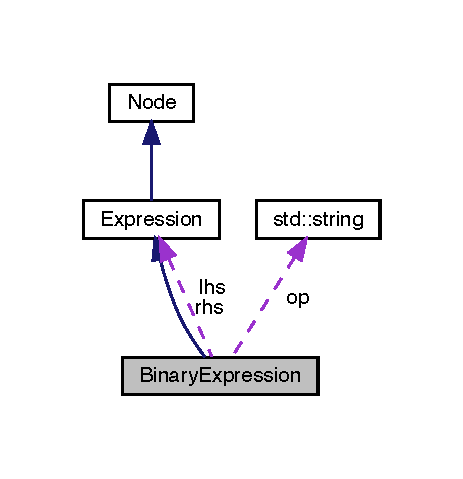
\includegraphics[width=174pt]{struct_binary_expression__coll__graph}
\end{center}
\end{figure}
\subsection*{Public Attributes}
\begin{DoxyCompactItemize}
\item 
\textbf{ std\+::string} \hyperlink{struct_binary_expression_a4c33b66e2ffc0a5ede2cdd190bf4bd75}{op}
\item 
\hyperlink{ast_8h_a4cb273a4d960cd13ea17d08f254493e8}{Expression} \hyperlink{struct_binary_expression_ab64ea2909c297e50015730abf814e82c}{lhs}
\item 
\hyperlink{ast_8h_a4cb273a4d960cd13ea17d08f254493e8}{Expression} \hyperlink{struct_binary_expression_aa25a00083ca8f135c0ffa46c527086a7}{rhs}
\end{DoxyCompactItemize}


\subsection{Member Data Documentation}
\mbox{\Hypertarget{struct_binary_expression_ab64ea2909c297e50015730abf814e82c}\label{struct_binary_expression_ab64ea2909c297e50015730abf814e82c}} 
\index{Binary\+Expression@{Binary\+Expression}!lhs@{lhs}}
\index{lhs@{lhs}!Binary\+Expression@{Binary\+Expression}}
\subsubsection{\texorpdfstring{lhs}{lhs}}
{\footnotesize\ttfamily \hyperlink{ast_8h_a4cb273a4d960cd13ea17d08f254493e8}{Expression} Binary\+Expression\+::lhs}

\mbox{\Hypertarget{struct_binary_expression_a4c33b66e2ffc0a5ede2cdd190bf4bd75}\label{struct_binary_expression_a4c33b66e2ffc0a5ede2cdd190bf4bd75}} 
\index{Binary\+Expression@{Binary\+Expression}!op@{op}}
\index{op@{op}!Binary\+Expression@{Binary\+Expression}}
\subsubsection{\texorpdfstring{op}{op}}
{\footnotesize\ttfamily \textbf{ std\+::string} Binary\+Expression\+::op}

\mbox{\Hypertarget{struct_binary_expression_aa25a00083ca8f135c0ffa46c527086a7}\label{struct_binary_expression_aa25a00083ca8f135c0ffa46c527086a7}} 
\index{Binary\+Expression@{Binary\+Expression}!rhs@{rhs}}
\index{rhs@{rhs}!Binary\+Expression@{Binary\+Expression}}
\subsubsection{\texorpdfstring{rhs}{rhs}}
{\footnotesize\ttfamily \hyperlink{ast_8h_a4cb273a4d960cd13ea17d08f254493e8}{Expression} Binary\+Expression\+::rhs}



The documentation for this struct was generated from the following file\+:\begin{DoxyCompactItemize}
\item 
src/\hyperlink{ast_8h}{ast.\+h}\end{DoxyCompactItemize}

\hypertarget{struct_block}{}\section{Block Struct Reference}
\label{struct_block}\index{Block@{Block}}


{\ttfamily \#include $<$ast.\+h$>$}



Inheritance diagram for Block\+:\nopagebreak
\begin{figure}[H]
\begin{center}
\leavevmode
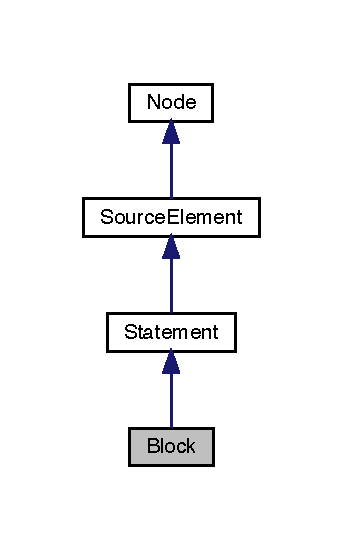
\includegraphics[width=164pt]{struct_block__inherit__graph}
\end{center}
\end{figure}


Collaboration diagram for Block\+:\nopagebreak
\begin{figure}[H]
\begin{center}
\leavevmode
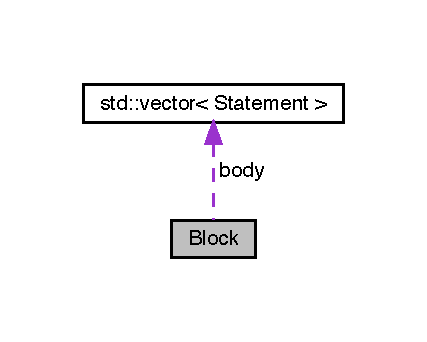
\includegraphics[width=294pt]{struct_block__coll__graph}
\end{center}
\end{figure}
\subsection*{Public Member Functions}
\begin{DoxyCompactItemize}
\item 
\hyperlink{struct_block_a757d46b60b5babb84c5c466b99679c2d}{Block} (\hyperlink{struct_statement_list}{Statement\+List} $\ast$\hyperlink{struct_block_a05207097167e9263252079d78f3d9358}{body}=nullptr)
\item 
void \hyperlink{struct_block_ac00e5c0ee8486dbdc7cb91dd5a6b34e1}{accept} (\hyperlink{struct_visitor}{Visitor} \&visitor) const override
\item 
const char $\ast$ \hyperlink{struct_block_a0a495712f07ce103494469c87a8352c2}{type} () const override
\end{DoxyCompactItemize}
\subsection*{Public Attributes}
\begin{DoxyCompactItemize}
\item 
\hyperlink{struct_statement_list}{Statement\+List} $\ast$ \hyperlink{struct_block_a05207097167e9263252079d78f3d9358}{body}
\end{DoxyCompactItemize}


\subsection{Constructor \& Destructor Documentation}
\mbox{\Hypertarget{struct_block_a757d46b60b5babb84c5c466b99679c2d}\label{struct_block_a757d46b60b5babb84c5c466b99679c2d}} 
\index{Block@{Block}!Block@{Block}}
\index{Block@{Block}!Block@{Block}}
\subsubsection{\texorpdfstring{Block()}{Block()}}
{\footnotesize\ttfamily Block\+::\+Block (\begin{DoxyParamCaption}\item[{\hyperlink{struct_statement_list}{Statement\+List} $\ast$}]{body = {\ttfamily nullptr} }\end{DoxyParamCaption})\hspace{0.3cm}{\ttfamily [inline]}}



\subsection{Member Function Documentation}
\mbox{\Hypertarget{struct_block_ac00e5c0ee8486dbdc7cb91dd5a6b34e1}\label{struct_block_ac00e5c0ee8486dbdc7cb91dd5a6b34e1}} 
\index{Block@{Block}!accept@{accept}}
\index{accept@{accept}!Block@{Block}}
\subsubsection{\texorpdfstring{accept()}{accept()}}
{\footnotesize\ttfamily void Block\+::accept (\begin{DoxyParamCaption}\item[{\hyperlink{struct_visitor}{Visitor} \&}]{visitor }\end{DoxyParamCaption}) const\hspace{0.3cm}{\ttfamily [inline]}, {\ttfamily [override]}, {\ttfamily [virtual]}}



Implements \hyperlink{struct_node_a10bd7af968140bbf5fa461298a969c71}{Node}.

\mbox{\Hypertarget{struct_block_a0a495712f07ce103494469c87a8352c2}\label{struct_block_a0a495712f07ce103494469c87a8352c2}} 
\index{Block@{Block}!type@{type}}
\index{type@{type}!Block@{Block}}
\subsubsection{\texorpdfstring{type()}{type()}}
{\footnotesize\ttfamily const char$\ast$ Block\+::type (\begin{DoxyParamCaption}{ }\end{DoxyParamCaption}) const\hspace{0.3cm}{\ttfamily [inline]}, {\ttfamily [override]}, {\ttfamily [virtual]}}



Implements \hyperlink{struct_node_a82f29420d0a38efcc370352528e94e9b}{Node}.



\subsection{Member Data Documentation}
\mbox{\Hypertarget{struct_block_a05207097167e9263252079d78f3d9358}\label{struct_block_a05207097167e9263252079d78f3d9358}} 
\index{Block@{Block}!body@{body}}
\index{body@{body}!Block@{Block}}
\subsubsection{\texorpdfstring{body}{body}}
{\footnotesize\ttfamily \hyperlink{struct_statement_list}{Statement\+List}$\ast$ Block\+::body}



The documentation for this struct was generated from the following file\+:\begin{DoxyCompactItemize}
\item 
src/\hyperlink{ast_8h}{ast.\+h}\end{DoxyCompactItemize}

\hypertarget{struct_boolean}{}\section{Boolean Struct Reference}
\label{struct_boolean}\index{Boolean@{Boolean}}


{\ttfamily \#include $<$value.\+h$>$}

\subsection*{Public Attributes}
\begin{DoxyCompactItemize}
\item 
bool \hyperlink{struct_boolean_a8e44c7f95d984f2dc8c6974f607b2b36}{value}
\end{DoxyCompactItemize}


\subsection{Member Data Documentation}
\mbox{\Hypertarget{struct_boolean_a8e44c7f95d984f2dc8c6974f607b2b36}\label{struct_boolean_a8e44c7f95d984f2dc8c6974f607b2b36}} 
\index{Boolean@{Boolean}!value@{value}}
\index{value@{value}!Boolean@{Boolean}}
\subsubsection{\texorpdfstring{value}{value}}
{\footnotesize\ttfamily bool Boolean\+::value}



The documentation for this struct was generated from the following file\+:\begin{DoxyCompactItemize}
\item 
src/\hyperlink{value_8h}{value.\+h}\end{DoxyCompactItemize}

\hypertarget{struct_boolean_literal}{}\section{Boolean\+Literal Struct Reference}
\label{struct_boolean_literal}\index{Boolean\+Literal@{Boolean\+Literal}}


{\ttfamily \#include $<$ast.\+h$>$}



Inheritance diagram for Boolean\+Literal\+:\nopagebreak
\begin{figure}[H]
\begin{center}
\leavevmode
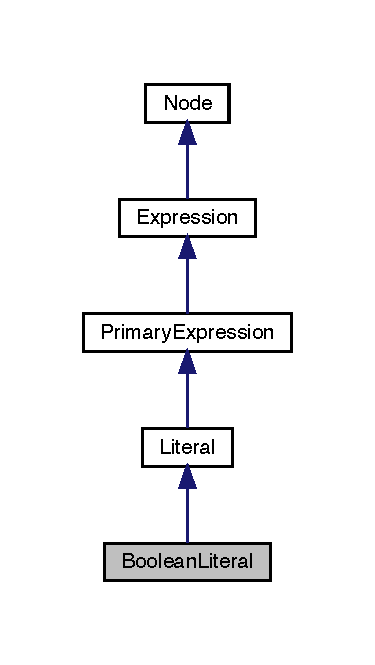
\includegraphics[width=160pt]{struct_boolean_literal__inherit__graph}
\end{center}
\end{figure}


Collaboration diagram for Boolean\+Literal\+:
\nopagebreak
\begin{figure}[H]
\begin{center}
\leavevmode
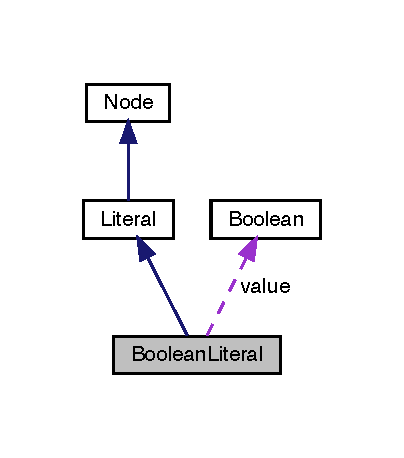
\includegraphics[width=194pt]{struct_boolean_literal__coll__graph}
\end{center}
\end{figure}
\subsection*{Public Member Functions}
\begin{DoxyCompactItemize}
\item 
\hyperlink{struct_boolean_literal_a62943a1e1523297b1ea0372d1a5fbbfb}{Boolean\+Literal} (\hyperlink{struct_boolean}{Boolean} \hyperlink{struct_boolean_literal_af74f8eba8c2ea30656de4c4919f5778d}{value})
\item 
void \hyperlink{struct_boolean_literal_aeb7a30e2b22ac6ad12723da1e72087c5}{accept} (\hyperlink{struct_visitor}{Visitor} \&visitor) const override
\item 
const char $\ast$ \hyperlink{struct_boolean_literal_aa10a3ecbeefe15607c3ac43ed63ba8da}{type} () const override
\end{DoxyCompactItemize}
\subsection*{Public Attributes}
\begin{DoxyCompactItemize}
\item 
\hyperlink{struct_boolean}{Boolean} \hyperlink{struct_boolean_literal_af74f8eba8c2ea30656de4c4919f5778d}{value}
\end{DoxyCompactItemize}


\subsection{Constructor \& Destructor Documentation}
\mbox{\Hypertarget{struct_boolean_literal_a62943a1e1523297b1ea0372d1a5fbbfb}\label{struct_boolean_literal_a62943a1e1523297b1ea0372d1a5fbbfb}} 
\index{Boolean\+Literal@{Boolean\+Literal}!Boolean\+Literal@{Boolean\+Literal}}
\index{Boolean\+Literal@{Boolean\+Literal}!Boolean\+Literal@{Boolean\+Literal}}
\subsubsection{\texorpdfstring{Boolean\+Literal()}{BooleanLiteral()}}
{\footnotesize\ttfamily Boolean\+Literal\+::\+Boolean\+Literal (\begin{DoxyParamCaption}\item[{\hyperlink{struct_boolean}{Boolean}}]{value }\end{DoxyParamCaption})\hspace{0.3cm}{\ttfamily [inline]}}



\subsection{Member Function Documentation}
\mbox{\Hypertarget{struct_boolean_literal_aeb7a30e2b22ac6ad12723da1e72087c5}\label{struct_boolean_literal_aeb7a30e2b22ac6ad12723da1e72087c5}} 
\index{Boolean\+Literal@{Boolean\+Literal}!accept@{accept}}
\index{accept@{accept}!Boolean\+Literal@{Boolean\+Literal}}
\subsubsection{\texorpdfstring{accept()}{accept()}}
{\footnotesize\ttfamily void Boolean\+Literal\+::accept (\begin{DoxyParamCaption}\item[{\hyperlink{struct_visitor}{Visitor} \&}]{visitor }\end{DoxyParamCaption}) const\hspace{0.3cm}{\ttfamily [inline]}, {\ttfamily [override]}, {\ttfamily [virtual]}}



Implements \hyperlink{struct_node_a10bd7af968140bbf5fa461298a969c71}{Node}.

\mbox{\Hypertarget{struct_boolean_literal_aa10a3ecbeefe15607c3ac43ed63ba8da}\label{struct_boolean_literal_aa10a3ecbeefe15607c3ac43ed63ba8da}} 
\index{Boolean\+Literal@{Boolean\+Literal}!type@{type}}
\index{type@{type}!Boolean\+Literal@{Boolean\+Literal}}
\subsubsection{\texorpdfstring{type()}{type()}}
{\footnotesize\ttfamily const char$\ast$ Boolean\+Literal\+::type (\begin{DoxyParamCaption}{ }\end{DoxyParamCaption}) const\hspace{0.3cm}{\ttfamily [inline]}, {\ttfamily [override]}, {\ttfamily [virtual]}}



Implements \hyperlink{struct_node_a82f29420d0a38efcc370352528e94e9b}{Node}.



\subsection{Member Data Documentation}
\mbox{\Hypertarget{struct_boolean_literal_af74f8eba8c2ea30656de4c4919f5778d}\label{struct_boolean_literal_af74f8eba8c2ea30656de4c4919f5778d}} 
\index{Boolean\+Literal@{Boolean\+Literal}!value@{value}}
\index{value@{value}!Boolean\+Literal@{Boolean\+Literal}}
\subsubsection{\texorpdfstring{value}{value}}
{\footnotesize\ttfamily \hyperlink{struct_boolean}{Boolean} Boolean\+Literal\+::value}



The documentation for this struct was generated from the following file\+:\begin{DoxyCompactItemize}
\item 
src/\hyperlink{ast_8h}{ast.\+h}\end{DoxyCompactItemize}

\hypertarget{struct_break_statement}{}\section{Break\+Statement Struct Reference}
\label{struct_break_statement}\index{Break\+Statement@{Break\+Statement}}


{\ttfamily \#include $<$ast.\+h$>$}

\subsection*{Public Attributes}
\begin{DoxyCompactItemize}
\item 
boost\+::optional$<$ \hyperlink{struct_identifier}{Identifier} $>$ \hyperlink{struct_break_statement_a0367fe642b46069be309b05e05b547c5}{label}
\end{DoxyCompactItemize}


\subsection{Member Data Documentation}
\mbox{\Hypertarget{struct_break_statement_a0367fe642b46069be309b05e05b547c5}\label{struct_break_statement_a0367fe642b46069be309b05e05b547c5}} 
\index{Break\+Statement@{Break\+Statement}!label@{label}}
\index{label@{label}!Break\+Statement@{Break\+Statement}}
\subsubsection{\texorpdfstring{label}{label}}
{\footnotesize\ttfamily boost\+::optional$<$\hyperlink{struct_identifier}{Identifier}$>$ Break\+Statement\+::label}



The documentation for this struct was generated from the following file\+:\begin{DoxyCompactItemize}
\item 
src/\hyperlink{ast_8h}{ast.\+h}\end{DoxyCompactItemize}

\hypertarget{struct_call_expression}{}\section{Call\+Expression Struct Reference}
\label{struct_call_expression}\index{Call\+Expression@{Call\+Expression}}


{\ttfamily \#include $<$ast.\+h$>$}



Inheritance diagram for Call\+Expression\+:
\nopagebreak
\begin{figure}[H]
\begin{center}
\leavevmode
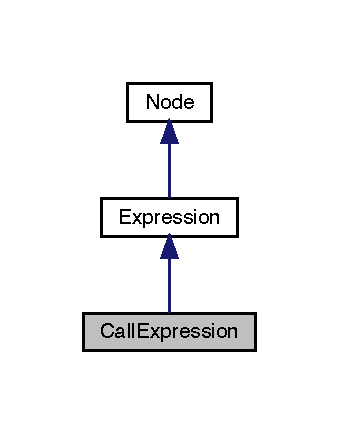
\includegraphics[width=163pt]{struct_call_expression__inherit__graph}
\end{center}
\end{figure}


Collaboration diagram for Call\+Expression\+:
\nopagebreak
\begin{figure}[H]
\begin{center}
\leavevmode
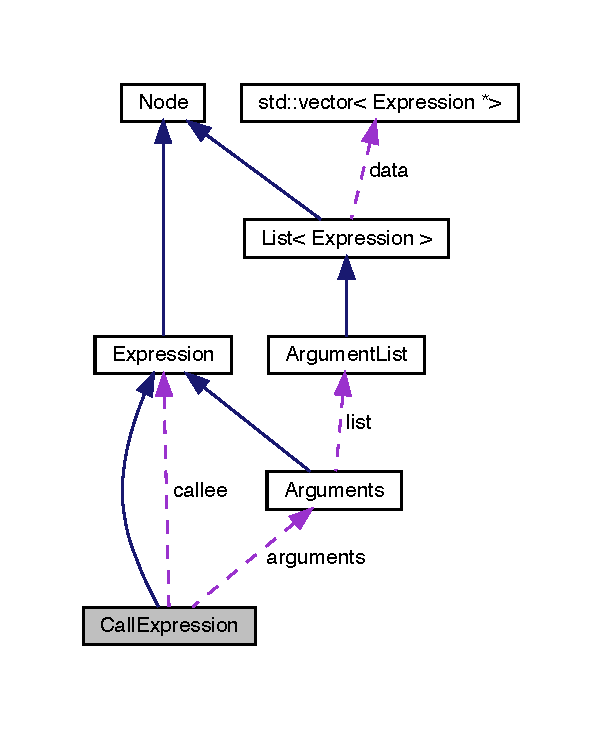
\includegraphics[width=289pt]{struct_call_expression__coll__graph}
\end{center}
\end{figure}
\subsection*{Public Member Functions}
\begin{DoxyCompactItemize}
\item 
\hyperlink{struct_call_expression_a7e6da0437a5f82430af5f31779b830d7}{Call\+Expression} (\hyperlink{struct_expression}{Expression} $\ast$\hyperlink{struct_call_expression_a2d77ccd1a2d6f34d718063f0eb47bc21}{callee}, \hyperlink{struct_arguments}{Arguments} $\ast$\hyperlink{struct_call_expression_ad2dad57df529ef1ef06b43cd438598bd}{arguments}=nullptr)
\item 
void \hyperlink{struct_call_expression_a5be626b61944a97f2a6015b632432513}{accept} (\hyperlink{struct_visitor}{Visitor} \&visitor) const override
\item 
const char $\ast$ \hyperlink{struct_call_expression_ae2891106618133745e00ac92a6b6b4fd}{type} () const override
\end{DoxyCompactItemize}
\subsection*{Public Attributes}
\begin{DoxyCompactItemize}
\item 
\hyperlink{struct_expression}{Expression} $\ast$ \hyperlink{struct_call_expression_a2d77ccd1a2d6f34d718063f0eb47bc21}{callee}
\item 
\hyperlink{struct_arguments}{Arguments} $\ast$ \hyperlink{struct_call_expression_ad2dad57df529ef1ef06b43cd438598bd}{arguments}
\end{DoxyCompactItemize}


\subsection{Constructor \& Destructor Documentation}
\mbox{\Hypertarget{struct_call_expression_a7e6da0437a5f82430af5f31779b830d7}\label{struct_call_expression_a7e6da0437a5f82430af5f31779b830d7}} 
\index{Call\+Expression@{Call\+Expression}!Call\+Expression@{Call\+Expression}}
\index{Call\+Expression@{Call\+Expression}!Call\+Expression@{Call\+Expression}}
\subsubsection{\texorpdfstring{Call\+Expression()}{CallExpression()}}
{\footnotesize\ttfamily Call\+Expression\+::\+Call\+Expression (\begin{DoxyParamCaption}\item[{\hyperlink{struct_expression}{Expression} $\ast$}]{callee,  }\item[{\hyperlink{struct_arguments}{Arguments} $\ast$}]{arguments = {\ttfamily nullptr} }\end{DoxyParamCaption})\hspace{0.3cm}{\ttfamily [inline]}}



\subsection{Member Function Documentation}
\mbox{\Hypertarget{struct_call_expression_a5be626b61944a97f2a6015b632432513}\label{struct_call_expression_a5be626b61944a97f2a6015b632432513}} 
\index{Call\+Expression@{Call\+Expression}!accept@{accept}}
\index{accept@{accept}!Call\+Expression@{Call\+Expression}}
\subsubsection{\texorpdfstring{accept()}{accept()}}
{\footnotesize\ttfamily void Call\+Expression\+::accept (\begin{DoxyParamCaption}\item[{\hyperlink{struct_visitor}{Visitor} \&}]{visitor }\end{DoxyParamCaption}) const\hspace{0.3cm}{\ttfamily [inline]}, {\ttfamily [override]}, {\ttfamily [virtual]}}



Implements \hyperlink{struct_node_a10bd7af968140bbf5fa461298a969c71}{Node}.

\mbox{\Hypertarget{struct_call_expression_ae2891106618133745e00ac92a6b6b4fd}\label{struct_call_expression_ae2891106618133745e00ac92a6b6b4fd}} 
\index{Call\+Expression@{Call\+Expression}!type@{type}}
\index{type@{type}!Call\+Expression@{Call\+Expression}}
\subsubsection{\texorpdfstring{type()}{type()}}
{\footnotesize\ttfamily const char$\ast$ Call\+Expression\+::type (\begin{DoxyParamCaption}{ }\end{DoxyParamCaption}) const\hspace{0.3cm}{\ttfamily [inline]}, {\ttfamily [override]}, {\ttfamily [virtual]}}



Implements \hyperlink{struct_node_a82f29420d0a38efcc370352528e94e9b}{Node}.



\subsection{Member Data Documentation}
\mbox{\Hypertarget{struct_call_expression_ad2dad57df529ef1ef06b43cd438598bd}\label{struct_call_expression_ad2dad57df529ef1ef06b43cd438598bd}} 
\index{Call\+Expression@{Call\+Expression}!arguments@{arguments}}
\index{arguments@{arguments}!Call\+Expression@{Call\+Expression}}
\subsubsection{\texorpdfstring{arguments}{arguments}}
{\footnotesize\ttfamily \hyperlink{struct_arguments}{Arguments}$\ast$ Call\+Expression\+::arguments}

\mbox{\Hypertarget{struct_call_expression_a2d77ccd1a2d6f34d718063f0eb47bc21}\label{struct_call_expression_a2d77ccd1a2d6f34d718063f0eb47bc21}} 
\index{Call\+Expression@{Call\+Expression}!callee@{callee}}
\index{callee@{callee}!Call\+Expression@{Call\+Expression}}
\subsubsection{\texorpdfstring{callee}{callee}}
{\footnotesize\ttfamily \hyperlink{struct_expression}{Expression}$\ast$ Call\+Expression\+::callee}



The documentation for this struct was generated from the following file\+:\begin{DoxyCompactItemize}
\item 
src/\hyperlink{ast_8h}{ast.\+h}\end{DoxyCompactItemize}

\hypertarget{struct_case_block}{}\section{Case\+Block Struct Reference}
\label{struct_case_block}\index{Case\+Block@{Case\+Block}}


{\ttfamily \#include $<$ast.\+h$>$}



Inheritance diagram for Case\+Block\+:\nopagebreak
\begin{figure}[H]
\begin{center}
\leavevmode
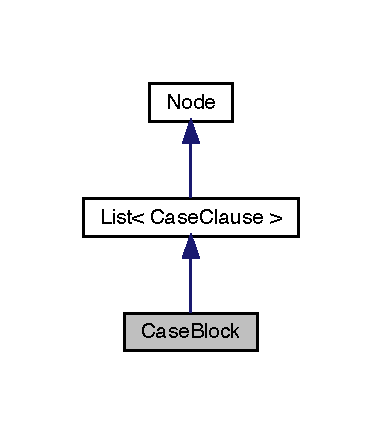
\includegraphics[width=183pt]{struct_case_block__inherit__graph}
\end{center}
\end{figure}


Collaboration diagram for Case\+Block\+:\nopagebreak
\begin{figure}[H]
\begin{center}
\leavevmode
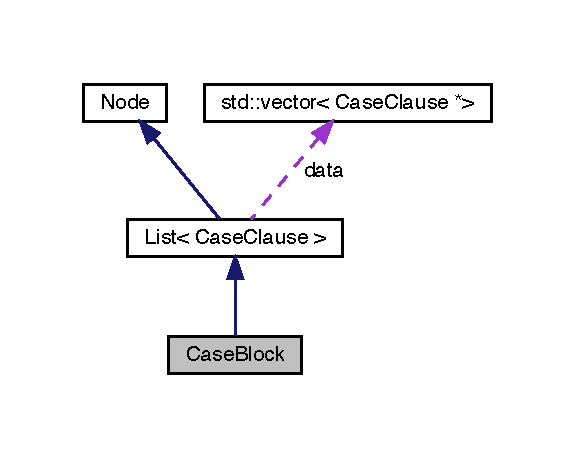
\includegraphics[width=276pt]{struct_case_block__coll__graph}
\end{center}
\end{figure}
\subsection*{Additional Inherited Members}


The documentation for this struct was generated from the following file\+:\begin{DoxyCompactItemize}
\item 
src/\hyperlink{ast_8h}{ast.\+h}\end{DoxyCompactItemize}

\hypertarget{struct_case_clause}{}\section{Case\+Clause Struct Reference}
\label{struct_case_clause}\index{Case\+Clause@{Case\+Clause}}


{\ttfamily \#include $<$ast.\+h$>$}



Inheritance diagram for Case\+Clause\+:\nopagebreak
\begin{figure}[H]
\begin{center}
\leavevmode
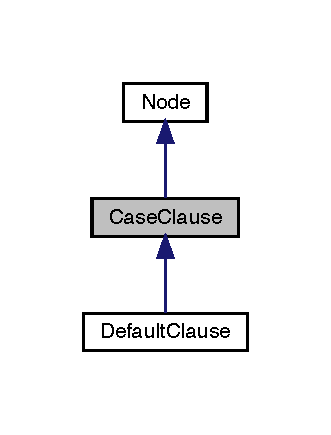
\includegraphics[width=159pt]{struct_case_clause__inherit__graph}
\end{center}
\end{figure}


Collaboration diagram for Case\+Clause\+:\nopagebreak
\begin{figure}[H]
\begin{center}
\leavevmode
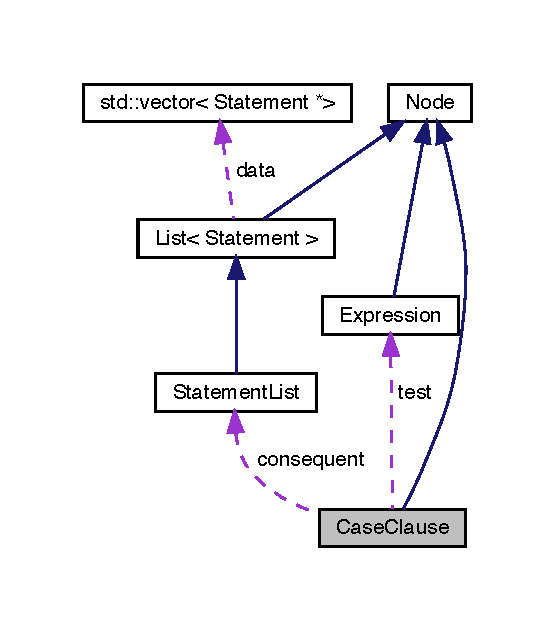
\includegraphics[width=266pt]{struct_case_clause__coll__graph}
\end{center}
\end{figure}
\subsection*{Public Member Functions}
\begin{DoxyCompactItemize}
\item 
\hyperlink{struct_case_clause_a05d8bf165e3a4796247b5fbf1f71d3e5}{Case\+Clause} (\hyperlink{struct_expression}{Expression} $\ast$\hyperlink{struct_case_clause_a80b6f256f3d9910250e4b8433ea75d7f}{test}, \hyperlink{struct_statement_list}{Statement\+List} $\ast$\hyperlink{struct_case_clause_a3e6914411610d1893b61172521e11288}{consequent})
\item 
void \hyperlink{struct_case_clause_a5bbee9ea9ca206c09b8b79f8c96720a1}{accept} (\hyperlink{struct_visitor}{Visitor} \&visitor) const override
\item 
const char $\ast$ \hyperlink{struct_case_clause_a9dcb0a1a072df7d577b272c6bbb3c6dc}{type} () const override
\item 
bool \hyperlink{struct_case_clause_a8ef15339531ef33d3ae335d96317b30a}{is\+\_\+default} () const
\end{DoxyCompactItemize}
\subsection*{Public Attributes}
\begin{DoxyCompactItemize}
\item 
\hyperlink{struct_expression}{Expression} $\ast$ \hyperlink{struct_case_clause_a80b6f256f3d9910250e4b8433ea75d7f}{test} = nullptr
\item 
\hyperlink{struct_statement_list}{Statement\+List} $\ast$ \hyperlink{struct_case_clause_a3e6914411610d1893b61172521e11288}{consequent}
\end{DoxyCompactItemize}


\subsection{Constructor \& Destructor Documentation}
\mbox{\Hypertarget{struct_case_clause_a05d8bf165e3a4796247b5fbf1f71d3e5}\label{struct_case_clause_a05d8bf165e3a4796247b5fbf1f71d3e5}} 
\index{Case\+Clause@{Case\+Clause}!Case\+Clause@{Case\+Clause}}
\index{Case\+Clause@{Case\+Clause}!Case\+Clause@{Case\+Clause}}
\subsubsection{\texorpdfstring{Case\+Clause()}{CaseClause()}}
{\footnotesize\ttfamily Case\+Clause\+::\+Case\+Clause (\begin{DoxyParamCaption}\item[{\hyperlink{struct_expression}{Expression} $\ast$}]{test,  }\item[{\hyperlink{struct_statement_list}{Statement\+List} $\ast$}]{consequent }\end{DoxyParamCaption})\hspace{0.3cm}{\ttfamily [inline]}}



\subsection{Member Function Documentation}
\mbox{\Hypertarget{struct_case_clause_a5bbee9ea9ca206c09b8b79f8c96720a1}\label{struct_case_clause_a5bbee9ea9ca206c09b8b79f8c96720a1}} 
\index{Case\+Clause@{Case\+Clause}!accept@{accept}}
\index{accept@{accept}!Case\+Clause@{Case\+Clause}}
\subsubsection{\texorpdfstring{accept()}{accept()}}
{\footnotesize\ttfamily void Case\+Clause\+::accept (\begin{DoxyParamCaption}\item[{\hyperlink{struct_visitor}{Visitor} \&}]{visitor }\end{DoxyParamCaption}) const\hspace{0.3cm}{\ttfamily [inline]}, {\ttfamily [override]}, {\ttfamily [virtual]}}



Implements \hyperlink{struct_node_a10bd7af968140bbf5fa461298a969c71}{Node}.



Reimplemented in \hyperlink{struct_default_clause_ade62e79cf9ad891d974528e1e172e2b6}{Default\+Clause}.

\mbox{\Hypertarget{struct_case_clause_a8ef15339531ef33d3ae335d96317b30a}\label{struct_case_clause_a8ef15339531ef33d3ae335d96317b30a}} 
\index{Case\+Clause@{Case\+Clause}!is\+\_\+default@{is\+\_\+default}}
\index{is\+\_\+default@{is\+\_\+default}!Case\+Clause@{Case\+Clause}}
\subsubsection{\texorpdfstring{is\+\_\+default()}{is\_default()}}
{\footnotesize\ttfamily bool Case\+Clause\+::is\+\_\+default (\begin{DoxyParamCaption}{ }\end{DoxyParamCaption}) const\hspace{0.3cm}{\ttfamily [inline]}}

\mbox{\Hypertarget{struct_case_clause_a9dcb0a1a072df7d577b272c6bbb3c6dc}\label{struct_case_clause_a9dcb0a1a072df7d577b272c6bbb3c6dc}} 
\index{Case\+Clause@{Case\+Clause}!type@{type}}
\index{type@{type}!Case\+Clause@{Case\+Clause}}
\subsubsection{\texorpdfstring{type()}{type()}}
{\footnotesize\ttfamily const char$\ast$ Case\+Clause\+::type (\begin{DoxyParamCaption}{ }\end{DoxyParamCaption}) const\hspace{0.3cm}{\ttfamily [inline]}, {\ttfamily [override]}, {\ttfamily [virtual]}}



Implements \hyperlink{struct_node_a82f29420d0a38efcc370352528e94e9b}{Node}.



Reimplemented in \hyperlink{struct_default_clause_a464358dcd7e4e13287482d3c858f3538}{Default\+Clause}.



\subsection{Member Data Documentation}
\mbox{\Hypertarget{struct_case_clause_a3e6914411610d1893b61172521e11288}\label{struct_case_clause_a3e6914411610d1893b61172521e11288}} 
\index{Case\+Clause@{Case\+Clause}!consequent@{consequent}}
\index{consequent@{consequent}!Case\+Clause@{Case\+Clause}}
\subsubsection{\texorpdfstring{consequent}{consequent}}
{\footnotesize\ttfamily \hyperlink{struct_statement_list}{Statement\+List}$\ast$ Case\+Clause\+::consequent}

\mbox{\Hypertarget{struct_case_clause_a80b6f256f3d9910250e4b8433ea75d7f}\label{struct_case_clause_a80b6f256f3d9910250e4b8433ea75d7f}} 
\index{Case\+Clause@{Case\+Clause}!test@{test}}
\index{test@{test}!Case\+Clause@{Case\+Clause}}
\subsubsection{\texorpdfstring{test}{test}}
{\footnotesize\ttfamily \hyperlink{struct_expression}{Expression}$\ast$ Case\+Clause\+::test = nullptr}



The documentation for this struct was generated from the following file\+:\begin{DoxyCompactItemize}
\item 
src/\hyperlink{ast_8h}{ast.\+h}\end{DoxyCompactItemize}

\hypertarget{struct_conditional_expression}{}\section{Conditional\+Expression Struct Reference}
\label{struct_conditional_expression}\index{Conditional\+Expression@{Conditional\+Expression}}


{\ttfamily \#include $<$ast.\+h$>$}



Inheritance diagram for Conditional\+Expression\+:\nopagebreak
\begin{figure}[H]
\begin{center}
\leavevmode
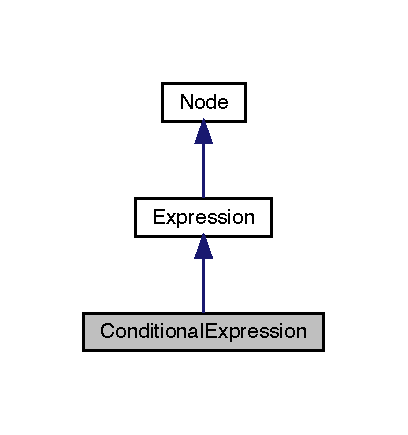
\includegraphics[width=196pt]{struct_conditional_expression__inherit__graph}
\end{center}
\end{figure}


Collaboration diagram for Conditional\+Expression\+:\nopagebreak
\begin{figure}[H]
\begin{center}
\leavevmode
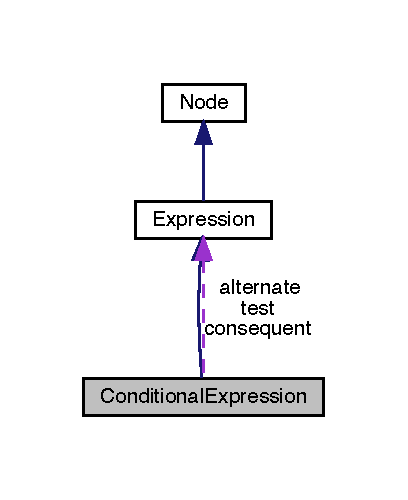
\includegraphics[width=196pt]{struct_conditional_expression__coll__graph}
\end{center}
\end{figure}
\subsection*{Public Member Functions}
\begin{DoxyCompactItemize}
\item 
\hyperlink{struct_conditional_expression_a37e1422b06b5533f67a85ceb92e9ae1e}{Conditional\+Expression} (\hyperlink{struct_expression}{Expression} $\ast$\hyperlink{struct_conditional_expression_a7bfe134769078a10eecccabba7405cc2}{test}, \hyperlink{struct_expression}{Expression} $\ast$\hyperlink{struct_conditional_expression_ac129a280df90c129183ec955f4e50ed0}{consequent}, \hyperlink{struct_expression}{Expression} $\ast$\hyperlink{struct_conditional_expression_aed7b09dab98000c8542d6353eefd8dac}{alternate})
\item 
void \hyperlink{struct_conditional_expression_af3883c99eba0226e3fbd424a672bcf7b}{accept} (\hyperlink{struct_visitor}{Visitor} \&visitor) const override
\end{DoxyCompactItemize}
\subsection*{Public Attributes}
\begin{DoxyCompactItemize}
\item 
\hyperlink{struct_expression}{Expression} $\ast$ \hyperlink{struct_conditional_expression_a7bfe134769078a10eecccabba7405cc2}{test}
\item 
\hyperlink{struct_expression}{Expression} $\ast$ \hyperlink{struct_conditional_expression_ac129a280df90c129183ec955f4e50ed0}{consequent}
\item 
\hyperlink{struct_expression}{Expression} $\ast$ \hyperlink{struct_conditional_expression_aed7b09dab98000c8542d6353eefd8dac}{alternate}
\end{DoxyCompactItemize}


\subsection{Constructor \& Destructor Documentation}
\mbox{\Hypertarget{struct_conditional_expression_a37e1422b06b5533f67a85ceb92e9ae1e}\label{struct_conditional_expression_a37e1422b06b5533f67a85ceb92e9ae1e}} 
\index{Conditional\+Expression@{Conditional\+Expression}!Conditional\+Expression@{Conditional\+Expression}}
\index{Conditional\+Expression@{Conditional\+Expression}!Conditional\+Expression@{Conditional\+Expression}}
\subsubsection{\texorpdfstring{Conditional\+Expression()}{ConditionalExpression()}}
{\footnotesize\ttfamily Conditional\+Expression\+::\+Conditional\+Expression (\begin{DoxyParamCaption}\item[{\hyperlink{struct_expression}{Expression} $\ast$}]{test,  }\item[{\hyperlink{struct_expression}{Expression} $\ast$}]{consequent,  }\item[{\hyperlink{struct_expression}{Expression} $\ast$}]{alternate }\end{DoxyParamCaption})\hspace{0.3cm}{\ttfamily [inline]}}



\subsection{Member Function Documentation}
\mbox{\Hypertarget{struct_conditional_expression_af3883c99eba0226e3fbd424a672bcf7b}\label{struct_conditional_expression_af3883c99eba0226e3fbd424a672bcf7b}} 
\index{Conditional\+Expression@{Conditional\+Expression}!accept@{accept}}
\index{accept@{accept}!Conditional\+Expression@{Conditional\+Expression}}
\subsubsection{\texorpdfstring{accept()}{accept()}}
{\footnotesize\ttfamily void Conditional\+Expression\+::accept (\begin{DoxyParamCaption}\item[{\hyperlink{struct_visitor}{Visitor} \&}]{visitor }\end{DoxyParamCaption}) const\hspace{0.3cm}{\ttfamily [inline]}, {\ttfamily [override]}, {\ttfamily [virtual]}}



Implements \hyperlink{struct_node_a10bd7af968140bbf5fa461298a969c71}{Node}.



\subsection{Member Data Documentation}
\mbox{\Hypertarget{struct_conditional_expression_aed7b09dab98000c8542d6353eefd8dac}\label{struct_conditional_expression_aed7b09dab98000c8542d6353eefd8dac}} 
\index{Conditional\+Expression@{Conditional\+Expression}!alternate@{alternate}}
\index{alternate@{alternate}!Conditional\+Expression@{Conditional\+Expression}}
\subsubsection{\texorpdfstring{alternate}{alternate}}
{\footnotesize\ttfamily \hyperlink{struct_expression}{Expression}$\ast$ Conditional\+Expression\+::alternate}

\mbox{\Hypertarget{struct_conditional_expression_ac129a280df90c129183ec955f4e50ed0}\label{struct_conditional_expression_ac129a280df90c129183ec955f4e50ed0}} 
\index{Conditional\+Expression@{Conditional\+Expression}!consequent@{consequent}}
\index{consequent@{consequent}!Conditional\+Expression@{Conditional\+Expression}}
\subsubsection{\texorpdfstring{consequent}{consequent}}
{\footnotesize\ttfamily \hyperlink{struct_expression}{Expression}$\ast$ Conditional\+Expression\+::consequent}

\mbox{\Hypertarget{struct_conditional_expression_a7bfe134769078a10eecccabba7405cc2}\label{struct_conditional_expression_a7bfe134769078a10eecccabba7405cc2}} 
\index{Conditional\+Expression@{Conditional\+Expression}!test@{test}}
\index{test@{test}!Conditional\+Expression@{Conditional\+Expression}}
\subsubsection{\texorpdfstring{test}{test}}
{\footnotesize\ttfamily \hyperlink{struct_expression}{Expression}$\ast$ Conditional\+Expression\+::test}



The documentation for this struct was generated from the following file\+:\begin{DoxyCompactItemize}
\item 
src/\hyperlink{ast_8h}{ast.\+h}\end{DoxyCompactItemize}

\hypertarget{struct_continue_statement}{}\section{Continue\+Statement Struct Reference}
\label{struct_continue_statement}\index{Continue\+Statement@{Continue\+Statement}}


{\ttfamily \#include $<$ast.\+h$>$}



Inheritance diagram for Continue\+Statement\+:\nopagebreak
\begin{figure}[H]
\begin{center}
\leavevmode
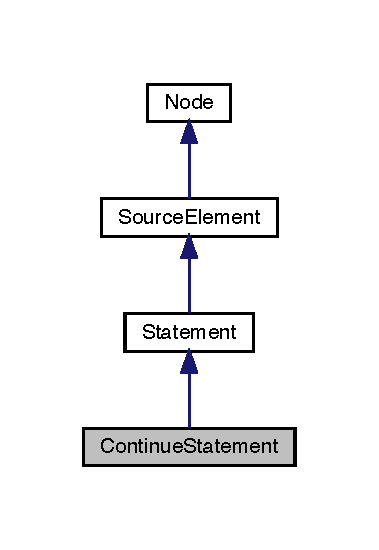
\includegraphics[width=182pt]{struct_continue_statement__inherit__graph}
\end{center}
\end{figure}


Collaboration diagram for Continue\+Statement\+:
\nopagebreak
\begin{figure}[H]
\begin{center}
\leavevmode
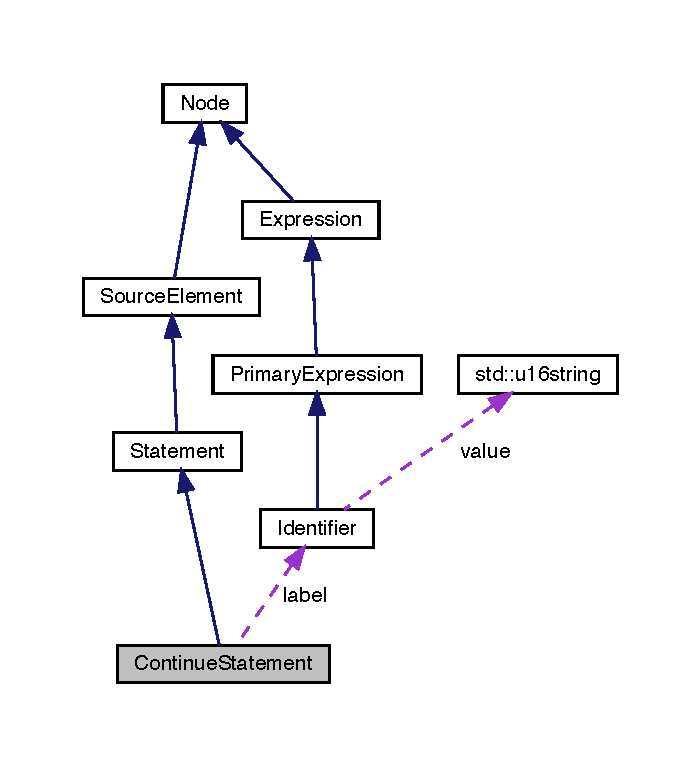
\includegraphics[width=247pt]{struct_continue_statement__coll__graph}
\end{center}
\end{figure}
\subsection*{Public Member Functions}
\begin{DoxyCompactItemize}
\item 
\hyperlink{struct_continue_statement_a45152addd01adf9e6d10c0af8505128c}{Continue\+Statement} (\hyperlink{struct_identifier}{Identifier} $\ast$\hyperlink{struct_continue_statement_a4bf8883a88736fa6ce4341e9029db194}{label}=nullptr)
\item 
void \hyperlink{struct_continue_statement_a9288fc77078160a2709a6329f1fe4838}{accept} (\hyperlink{struct_visitor}{Visitor} \&visitor) const override
\item 
const char $\ast$ \hyperlink{struct_continue_statement_a08b73034c5d273c3c4cbad00b252913f}{type} () const override
\end{DoxyCompactItemize}
\subsection*{Public Attributes}
\begin{DoxyCompactItemize}
\item 
\hyperlink{struct_identifier}{Identifier} $\ast$ \hyperlink{struct_continue_statement_a4bf8883a88736fa6ce4341e9029db194}{label}
\end{DoxyCompactItemize}


\subsection{Constructor \& Destructor Documentation}
\mbox{\Hypertarget{struct_continue_statement_a45152addd01adf9e6d10c0af8505128c}\label{struct_continue_statement_a45152addd01adf9e6d10c0af8505128c}} 
\index{Continue\+Statement@{Continue\+Statement}!Continue\+Statement@{Continue\+Statement}}
\index{Continue\+Statement@{Continue\+Statement}!Continue\+Statement@{Continue\+Statement}}
\subsubsection{\texorpdfstring{Continue\+Statement()}{ContinueStatement()}}
{\footnotesize\ttfamily Continue\+Statement\+::\+Continue\+Statement (\begin{DoxyParamCaption}\item[{\hyperlink{struct_identifier}{Identifier} $\ast$}]{label = {\ttfamily nullptr} }\end{DoxyParamCaption})\hspace{0.3cm}{\ttfamily [inline]}}



\subsection{Member Function Documentation}
\mbox{\Hypertarget{struct_continue_statement_a9288fc77078160a2709a6329f1fe4838}\label{struct_continue_statement_a9288fc77078160a2709a6329f1fe4838}} 
\index{Continue\+Statement@{Continue\+Statement}!accept@{accept}}
\index{accept@{accept}!Continue\+Statement@{Continue\+Statement}}
\subsubsection{\texorpdfstring{accept()}{accept()}}
{\footnotesize\ttfamily void Continue\+Statement\+::accept (\begin{DoxyParamCaption}\item[{\hyperlink{struct_visitor}{Visitor} \&}]{visitor }\end{DoxyParamCaption}) const\hspace{0.3cm}{\ttfamily [inline]}, {\ttfamily [override]}, {\ttfamily [virtual]}}



Implements \hyperlink{struct_node_a10bd7af968140bbf5fa461298a969c71}{Node}.

\mbox{\Hypertarget{struct_continue_statement_a08b73034c5d273c3c4cbad00b252913f}\label{struct_continue_statement_a08b73034c5d273c3c4cbad00b252913f}} 
\index{Continue\+Statement@{Continue\+Statement}!type@{type}}
\index{type@{type}!Continue\+Statement@{Continue\+Statement}}
\subsubsection{\texorpdfstring{type()}{type()}}
{\footnotesize\ttfamily const char$\ast$ Continue\+Statement\+::type (\begin{DoxyParamCaption}{ }\end{DoxyParamCaption}) const\hspace{0.3cm}{\ttfamily [inline]}, {\ttfamily [override]}, {\ttfamily [virtual]}}



Implements \hyperlink{struct_node_a82f29420d0a38efcc370352528e94e9b}{Node}.



\subsection{Member Data Documentation}
\mbox{\Hypertarget{struct_continue_statement_a4bf8883a88736fa6ce4341e9029db194}\label{struct_continue_statement_a4bf8883a88736fa6ce4341e9029db194}} 
\index{Continue\+Statement@{Continue\+Statement}!label@{label}}
\index{label@{label}!Continue\+Statement@{Continue\+Statement}}
\subsubsection{\texorpdfstring{label}{label}}
{\footnotesize\ttfamily \hyperlink{struct_identifier}{Identifier}$\ast$ Continue\+Statement\+::label}



The documentation for this struct was generated from the following file\+:\begin{DoxyCompactItemize}
\item 
src/\hyperlink{ast_8h}{ast.\+h}\end{DoxyCompactItemize}

\hypertarget{struct_debugger_statement}{}\section{Debugger\+Statement Struct Reference}
\label{struct_debugger_statement}\index{Debugger\+Statement@{Debugger\+Statement}}


{\ttfamily \#include $<$ast.\+h$>$}



Inheritance diagram for Debugger\+Statement\+:\nopagebreak
\begin{figure}[H]
\begin{center}
\leavevmode
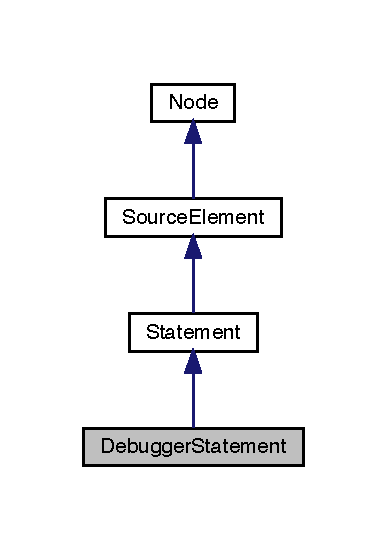
\includegraphics[width=186pt]{struct_debugger_statement__inherit__graph}
\end{center}
\end{figure}


Collaboration diagram for Debugger\+Statement\+:\nopagebreak
\begin{figure}[H]
\begin{center}
\leavevmode
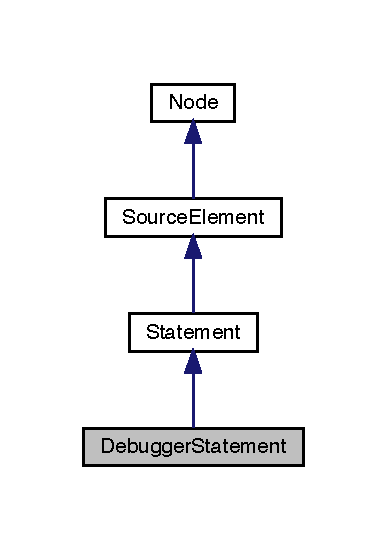
\includegraphics[width=186pt]{struct_debugger_statement__coll__graph}
\end{center}
\end{figure}
\subsection*{Public Member Functions}
\begin{DoxyCompactItemize}
\item 
void \hyperlink{struct_debugger_statement_adb69027b0b27e1a8f74f4ddea5957799}{accept} (\hyperlink{struct_visitor}{Visitor} \&visitor) const override
\item 
const char $\ast$ \hyperlink{struct_debugger_statement_a3484d4e9900b72324bf5eb55da9492dd}{type} () const override
\end{DoxyCompactItemize}


\subsection{Member Function Documentation}
\mbox{\Hypertarget{struct_debugger_statement_adb69027b0b27e1a8f74f4ddea5957799}\label{struct_debugger_statement_adb69027b0b27e1a8f74f4ddea5957799}} 
\index{Debugger\+Statement@{Debugger\+Statement}!accept@{accept}}
\index{accept@{accept}!Debugger\+Statement@{Debugger\+Statement}}
\subsubsection{\texorpdfstring{accept()}{accept()}}
{\footnotesize\ttfamily void Debugger\+Statement\+::accept (\begin{DoxyParamCaption}\item[{\hyperlink{struct_visitor}{Visitor} \&}]{visitor }\end{DoxyParamCaption}) const\hspace{0.3cm}{\ttfamily [inline]}, {\ttfamily [override]}, {\ttfamily [virtual]}}



Implements \hyperlink{struct_node_a10bd7af968140bbf5fa461298a969c71}{Node}.

\mbox{\Hypertarget{struct_debugger_statement_a3484d4e9900b72324bf5eb55da9492dd}\label{struct_debugger_statement_a3484d4e9900b72324bf5eb55da9492dd}} 
\index{Debugger\+Statement@{Debugger\+Statement}!type@{type}}
\index{type@{type}!Debugger\+Statement@{Debugger\+Statement}}
\subsubsection{\texorpdfstring{type()}{type()}}
{\footnotesize\ttfamily const char$\ast$ Debugger\+Statement\+::type (\begin{DoxyParamCaption}{ }\end{DoxyParamCaption}) const\hspace{0.3cm}{\ttfamily [inline]}, {\ttfamily [override]}, {\ttfamily [virtual]}}



Implements \hyperlink{struct_node_a82f29420d0a38efcc370352528e94e9b}{Node}.



The documentation for this struct was generated from the following file\+:\begin{DoxyCompactItemize}
\item 
src/\hyperlink{ast_8h}{ast.\+h}\end{DoxyCompactItemize}

\hypertarget{struct_token_1_1_debug_info}{}\section{Token\+:\+:Debug\+Info Struct Reference}
\label{struct_token_1_1_debug_info}\index{Token\+::\+Debug\+Info@{Token\+::\+Debug\+Info}}


{\ttfamily \#include $<$token.\+h$>$}

\subsection*{Public Member Functions}
\begin{DoxyCompactItemize}
\item 
virtual \textbf{ std\+::string} \hyperlink{struct_token_1_1_debug_info_a4d66aa65422c236198bbcc616bba250f}{syntax\+\_\+error\+\_\+at} () const =0
\item 
virtual \textbf{ std\+::string} \hyperlink{struct_token_1_1_debug_info_a0860d9b875240dafa0e00756d27e55bb}{loc} () const =0
\end{DoxyCompactItemize}


\subsection{Member Function Documentation}
\mbox{\Hypertarget{struct_token_1_1_debug_info_a0860d9b875240dafa0e00756d27e55bb}\label{struct_token_1_1_debug_info_a0860d9b875240dafa0e00756d27e55bb}} 
\index{Token\+::\+Debug\+Info@{Token\+::\+Debug\+Info}!loc@{loc}}
\index{loc@{loc}!Token\+::\+Debug\+Info@{Token\+::\+Debug\+Info}}
\subsubsection{\texorpdfstring{loc()}{loc()}}
{\footnotesize\ttfamily virtual \textbf{ std\+::string} Token\+::\+Debug\+Info\+::loc (\begin{DoxyParamCaption}{ }\end{DoxyParamCaption}) const\hspace{0.3cm}{\ttfamily [pure virtual]}}

\mbox{\Hypertarget{struct_token_1_1_debug_info_a4d66aa65422c236198bbcc616bba250f}\label{struct_token_1_1_debug_info_a4d66aa65422c236198bbcc616bba250f}} 
\index{Token\+::\+Debug\+Info@{Token\+::\+Debug\+Info}!syntax\+\_\+error\+\_\+at@{syntax\+\_\+error\+\_\+at}}
\index{syntax\+\_\+error\+\_\+at@{syntax\+\_\+error\+\_\+at}!Token\+::\+Debug\+Info@{Token\+::\+Debug\+Info}}
\subsubsection{\texorpdfstring{syntax\+\_\+error\+\_\+at()}{syntax\_error\_at()}}
{\footnotesize\ttfamily virtual \textbf{ std\+::string} Token\+::\+Debug\+Info\+::syntax\+\_\+error\+\_\+at (\begin{DoxyParamCaption}{ }\end{DoxyParamCaption}) const\hspace{0.3cm}{\ttfamily [pure virtual]}}



The documentation for this struct was generated from the following file\+:\begin{DoxyCompactItemize}
\item 
src/\hyperlink{token_8h}{token.\+h}\end{DoxyCompactItemize}

\hypertarget{struct_declaration}{}\section{Declaration Struct Reference}
\label{struct_declaration}\index{Declaration@{Declaration}}


{\ttfamily \#include $<$ast.\+h$>$}



Inheritance diagram for Declaration\+:
\nopagebreak
\begin{figure}[H]
\begin{center}
\leavevmode
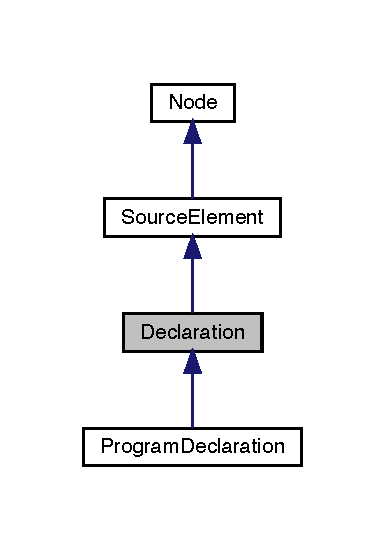
\includegraphics[width=185pt]{struct_declaration__inherit__graph}
\end{center}
\end{figure}


Collaboration diagram for Declaration\+:
\nopagebreak
\begin{figure}[H]
\begin{center}
\leavevmode
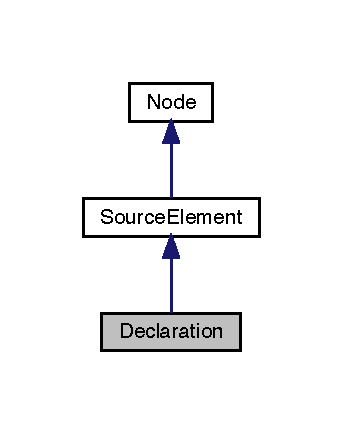
\includegraphics[width=164pt]{struct_declaration__coll__graph}
\end{center}
\end{figure}
\subsection*{Additional Inherited Members}


The documentation for this struct was generated from the following file\+:\begin{DoxyCompactItemize}
\item 
src/\hyperlink{ast_8h}{ast.\+h}\end{DoxyCompactItemize}

\hypertarget{struct_default_clause}{}\section{Default\+Clause Struct Reference}
\label{struct_default_clause}\index{Default\+Clause@{Default\+Clause}}


{\ttfamily \#include $<$ast.\+h$>$}



Inheritance diagram for Default\+Clause\+:\nopagebreak
\begin{figure}[H]
\begin{center}
\leavevmode
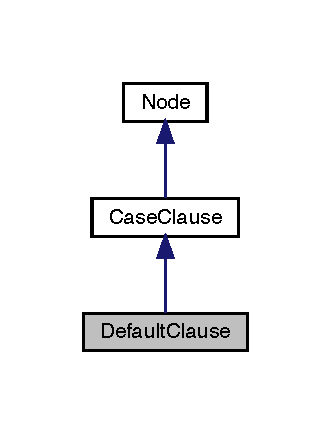
\includegraphics[width=159pt]{struct_default_clause__inherit__graph}
\end{center}
\end{figure}


Collaboration diagram for Default\+Clause\+:\nopagebreak
\begin{figure}[H]
\begin{center}
\leavevmode
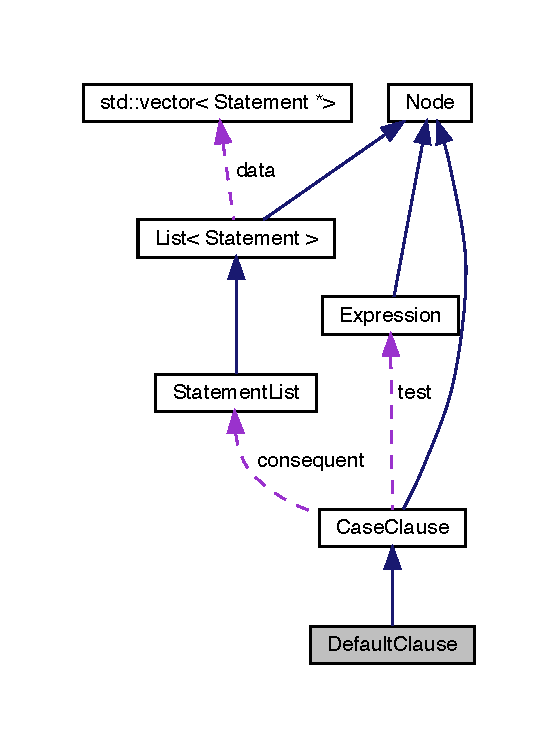
\includegraphics[width=268pt]{struct_default_clause__coll__graph}
\end{center}
\end{figure}
\subsection*{Public Member Functions}
\begin{DoxyCompactItemize}
\item 
\hyperlink{struct_default_clause_a9f15e6fc45dc6e8a3d87a02aa4798b25}{Default\+Clause} (\hyperlink{struct_statement_list}{Statement\+List} $\ast$\hyperlink{struct_case_clause_a3e6914411610d1893b61172521e11288}{consequent})
\item 
void \hyperlink{struct_default_clause_ade62e79cf9ad891d974528e1e172e2b6}{accept} (\hyperlink{struct_visitor}{Visitor} \&visitor) const override
\item 
const char $\ast$ \hyperlink{struct_default_clause_a464358dcd7e4e13287482d3c858f3538}{type} () const override
\end{DoxyCompactItemize}
\subsection*{Additional Inherited Members}


\subsection{Constructor \& Destructor Documentation}
\mbox{\Hypertarget{struct_default_clause_a9f15e6fc45dc6e8a3d87a02aa4798b25}\label{struct_default_clause_a9f15e6fc45dc6e8a3d87a02aa4798b25}} 
\index{Default\+Clause@{Default\+Clause}!Default\+Clause@{Default\+Clause}}
\index{Default\+Clause@{Default\+Clause}!Default\+Clause@{Default\+Clause}}
\subsubsection{\texorpdfstring{Default\+Clause()}{DefaultClause()}}
{\footnotesize\ttfamily Default\+Clause\+::\+Default\+Clause (\begin{DoxyParamCaption}\item[{\hyperlink{struct_statement_list}{Statement\+List} $\ast$}]{consequent }\end{DoxyParamCaption})\hspace{0.3cm}{\ttfamily [inline]}}



\subsection{Member Function Documentation}
\mbox{\Hypertarget{struct_default_clause_ade62e79cf9ad891d974528e1e172e2b6}\label{struct_default_clause_ade62e79cf9ad891d974528e1e172e2b6}} 
\index{Default\+Clause@{Default\+Clause}!accept@{accept}}
\index{accept@{accept}!Default\+Clause@{Default\+Clause}}
\subsubsection{\texorpdfstring{accept()}{accept()}}
{\footnotesize\ttfamily void Default\+Clause\+::accept (\begin{DoxyParamCaption}\item[{\hyperlink{struct_visitor}{Visitor} \&}]{visitor }\end{DoxyParamCaption}) const\hspace{0.3cm}{\ttfamily [inline]}, {\ttfamily [override]}, {\ttfamily [virtual]}}



Reimplemented from \hyperlink{struct_case_clause_a5bbee9ea9ca206c09b8b79f8c96720a1}{Case\+Clause}.

\mbox{\Hypertarget{struct_default_clause_a464358dcd7e4e13287482d3c858f3538}\label{struct_default_clause_a464358dcd7e4e13287482d3c858f3538}} 
\index{Default\+Clause@{Default\+Clause}!type@{type}}
\index{type@{type}!Default\+Clause@{Default\+Clause}}
\subsubsection{\texorpdfstring{type()}{type()}}
{\footnotesize\ttfamily const char$\ast$ Default\+Clause\+::type (\begin{DoxyParamCaption}{ }\end{DoxyParamCaption}) const\hspace{0.3cm}{\ttfamily [inline]}, {\ttfamily [override]}, {\ttfamily [virtual]}}



Reimplemented from \hyperlink{struct_case_clause_a9dcb0a1a072df7d577b272c6bbb3c6dc}{Case\+Clause}.



The documentation for this struct was generated from the following file\+:\begin{DoxyCompactItemize}
\item 
src/\hyperlink{ast_8h}{ast.\+h}\end{DoxyCompactItemize}

\hypertarget{struct_do_while_statement}{}\section{Do\+While\+Statement Struct Reference}
\label{struct_do_while_statement}\index{Do\+While\+Statement@{Do\+While\+Statement}}


{\ttfamily \#include $<$ast.\+h$>$}



Inheritance diagram for Do\+While\+Statement\+:\nopagebreak
\begin{figure}[H]
\begin{center}
\leavevmode
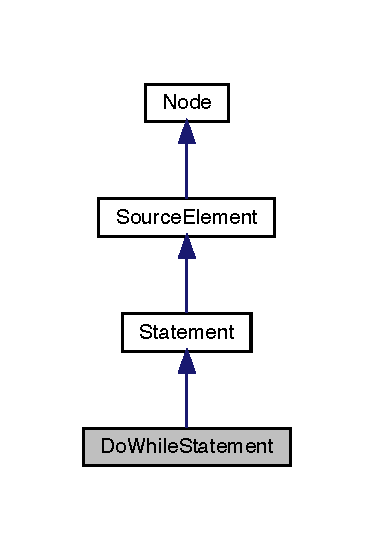
\includegraphics[width=179pt]{struct_do_while_statement__inherit__graph}
\end{center}
\end{figure}


Collaboration diagram for Do\+While\+Statement\+:\nopagebreak
\begin{figure}[H]
\begin{center}
\leavevmode
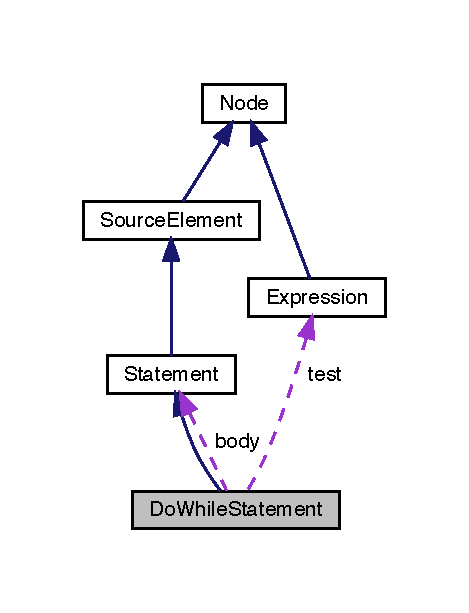
\includegraphics[width=225pt]{struct_do_while_statement__coll__graph}
\end{center}
\end{figure}
\subsection*{Public Member Functions}
\begin{DoxyCompactItemize}
\item 
\hyperlink{struct_do_while_statement_a26ed6b1502f71b59ac3cdfcfa3b7d07a}{Do\+While\+Statement} (\hyperlink{struct_statement}{Statement} $\ast$\hyperlink{struct_do_while_statement_a1742b816c78d6cfd511e69317461b52a}{body}, \hyperlink{struct_expression}{Expression} $\ast$\hyperlink{struct_do_while_statement_acd80c72a8d08b897462572fcce19fa42}{test})
\item 
void \hyperlink{struct_do_while_statement_afa4ddac75d1899fa41a134a49aa9c48f}{accept} (\hyperlink{struct_visitor}{Visitor} \&visitor) const override
\item 
const char $\ast$ \hyperlink{struct_do_while_statement_a91437b71a28b99c4cef7086dd89033ac}{type} () const override
\end{DoxyCompactItemize}
\subsection*{Public Attributes}
\begin{DoxyCompactItemize}
\item 
\hyperlink{struct_statement}{Statement} $\ast$ \hyperlink{struct_do_while_statement_a1742b816c78d6cfd511e69317461b52a}{body}
\item 
\hyperlink{struct_expression}{Expression} $\ast$ \hyperlink{struct_do_while_statement_acd80c72a8d08b897462572fcce19fa42}{test}
\end{DoxyCompactItemize}


\subsection{Constructor \& Destructor Documentation}
\mbox{\Hypertarget{struct_do_while_statement_a26ed6b1502f71b59ac3cdfcfa3b7d07a}\label{struct_do_while_statement_a26ed6b1502f71b59ac3cdfcfa3b7d07a}} 
\index{Do\+While\+Statement@{Do\+While\+Statement}!Do\+While\+Statement@{Do\+While\+Statement}}
\index{Do\+While\+Statement@{Do\+While\+Statement}!Do\+While\+Statement@{Do\+While\+Statement}}
\subsubsection{\texorpdfstring{Do\+While\+Statement()}{DoWhileStatement()}}
{\footnotesize\ttfamily Do\+While\+Statement\+::\+Do\+While\+Statement (\begin{DoxyParamCaption}\item[{\hyperlink{struct_statement}{Statement} $\ast$}]{body,  }\item[{\hyperlink{struct_expression}{Expression} $\ast$}]{test }\end{DoxyParamCaption})\hspace{0.3cm}{\ttfamily [inline]}}



\subsection{Member Function Documentation}
\mbox{\Hypertarget{struct_do_while_statement_afa4ddac75d1899fa41a134a49aa9c48f}\label{struct_do_while_statement_afa4ddac75d1899fa41a134a49aa9c48f}} 
\index{Do\+While\+Statement@{Do\+While\+Statement}!accept@{accept}}
\index{accept@{accept}!Do\+While\+Statement@{Do\+While\+Statement}}
\subsubsection{\texorpdfstring{accept()}{accept()}}
{\footnotesize\ttfamily void Do\+While\+Statement\+::accept (\begin{DoxyParamCaption}\item[{\hyperlink{struct_visitor}{Visitor} \&}]{visitor }\end{DoxyParamCaption}) const\hspace{0.3cm}{\ttfamily [inline]}, {\ttfamily [override]}, {\ttfamily [virtual]}}



Implements \hyperlink{struct_node_a10bd7af968140bbf5fa461298a969c71}{Node}.

\mbox{\Hypertarget{struct_do_while_statement_a91437b71a28b99c4cef7086dd89033ac}\label{struct_do_while_statement_a91437b71a28b99c4cef7086dd89033ac}} 
\index{Do\+While\+Statement@{Do\+While\+Statement}!type@{type}}
\index{type@{type}!Do\+While\+Statement@{Do\+While\+Statement}}
\subsubsection{\texorpdfstring{type()}{type()}}
{\footnotesize\ttfamily const char$\ast$ Do\+While\+Statement\+::type (\begin{DoxyParamCaption}{ }\end{DoxyParamCaption}) const\hspace{0.3cm}{\ttfamily [inline]}, {\ttfamily [override]}, {\ttfamily [virtual]}}



Implements \hyperlink{struct_node_a82f29420d0a38efcc370352528e94e9b}{Node}.



\subsection{Member Data Documentation}
\mbox{\Hypertarget{struct_do_while_statement_a1742b816c78d6cfd511e69317461b52a}\label{struct_do_while_statement_a1742b816c78d6cfd511e69317461b52a}} 
\index{Do\+While\+Statement@{Do\+While\+Statement}!body@{body}}
\index{body@{body}!Do\+While\+Statement@{Do\+While\+Statement}}
\subsubsection{\texorpdfstring{body}{body}}
{\footnotesize\ttfamily \hyperlink{struct_statement}{Statement}$\ast$ Do\+While\+Statement\+::body}

\mbox{\Hypertarget{struct_do_while_statement_acd80c72a8d08b897462572fcce19fa42}\label{struct_do_while_statement_acd80c72a8d08b897462572fcce19fa42}} 
\index{Do\+While\+Statement@{Do\+While\+Statement}!test@{test}}
\index{test@{test}!Do\+While\+Statement@{Do\+While\+Statement}}
\subsubsection{\texorpdfstring{test}{test}}
{\footnotesize\ttfamily \hyperlink{struct_expression}{Expression}$\ast$ Do\+While\+Statement\+::test}



The documentation for this struct was generated from the following file\+:\begin{DoxyCompactItemize}
\item 
src/\hyperlink{ast_8h}{ast.\+h}\end{DoxyCompactItemize}

\hypertarget{struct_element_list}{}\section{Element\+List Struct Reference}
\label{struct_element_list}\index{Element\+List@{Element\+List}}


{\ttfamily \#include $<$ast.\+h$>$}



Inheritance diagram for Element\+List\+:
\nopagebreak
\begin{figure}[H]
\begin{center}
\leavevmode
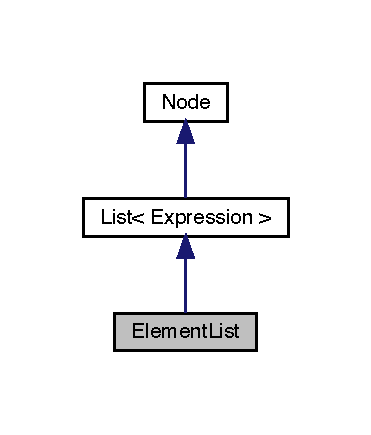
\includegraphics[width=153pt]{struct_element_list__inherit__graph}
\end{center}
\end{figure}


Collaboration diagram for Element\+List\+:
\nopagebreak
\begin{figure}[H]
\begin{center}
\leavevmode
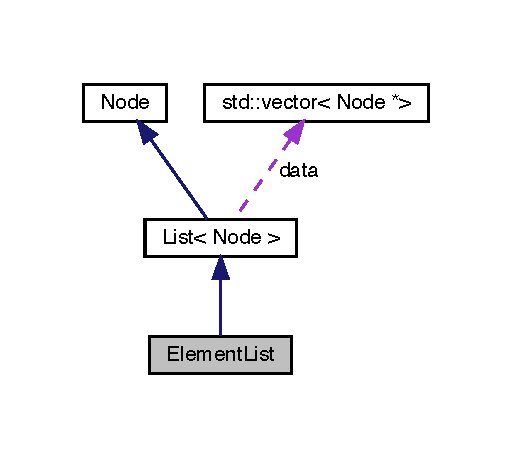
\includegraphics[width=246pt]{struct_element_list__coll__graph}
\end{center}
\end{figure}
\subsection*{Public Member Functions}
\begin{DoxyCompactItemize}
\item 
void \hyperlink{struct_element_list_a18e97e7ffed161a8f3f6a631550486fe}{accept} (\hyperlink{struct_visitor}{Visitor} \&visitor) const override
\item 
const char $\ast$ \hyperlink{struct_element_list_ae1da6b963a837e315c28dd017afc06a7}{type} () const override
\end{DoxyCompactItemize}
\subsection*{Additional Inherited Members}


\subsection{Member Function Documentation}
\mbox{\Hypertarget{struct_element_list_a18e97e7ffed161a8f3f6a631550486fe}\label{struct_element_list_a18e97e7ffed161a8f3f6a631550486fe}} 
\index{Element\+List@{Element\+List}!accept@{accept}}
\index{accept@{accept}!Element\+List@{Element\+List}}
\subsubsection{\texorpdfstring{accept()}{accept()}}
{\footnotesize\ttfamily void Element\+List\+::accept (\begin{DoxyParamCaption}\item[{\hyperlink{struct_visitor}{Visitor} \&}]{visitor }\end{DoxyParamCaption}) const\hspace{0.3cm}{\ttfamily [inline]}, {\ttfamily [override]}, {\ttfamily [virtual]}}



Implements \hyperlink{struct_node_a10bd7af968140bbf5fa461298a969c71}{Node}.

\mbox{\Hypertarget{struct_element_list_ae1da6b963a837e315c28dd017afc06a7}\label{struct_element_list_ae1da6b963a837e315c28dd017afc06a7}} 
\index{Element\+List@{Element\+List}!type@{type}}
\index{type@{type}!Element\+List@{Element\+List}}
\subsubsection{\texorpdfstring{type()}{type()}}
{\footnotesize\ttfamily const char$\ast$ Element\+List\+::type (\begin{DoxyParamCaption}{ }\end{DoxyParamCaption}) const\hspace{0.3cm}{\ttfamily [inline]}, {\ttfamily [override]}, {\ttfamily [virtual]}}



Implements \hyperlink{struct_node_a82f29420d0a38efcc370352528e94e9b}{Node}.



The documentation for this struct was generated from the following file\+:\begin{DoxyCompactItemize}
\item 
src/\hyperlink{ast_8h}{ast.\+h}\end{DoxyCompactItemize}

\hypertarget{struct_elision}{}\section{Elision Struct Reference}
\label{struct_elision}\index{Elision@{Elision}}


{\ttfamily \#include $<$ast.\+h$>$}



Inheritance diagram for Elision\+:\nopagebreak
\begin{figure}[H]
\begin{center}
\leavevmode
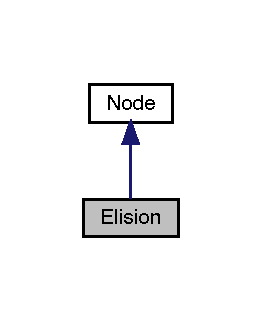
\includegraphics[width=145pt]{struct_elision__inherit__graph}
\end{center}
\end{figure}


Collaboration diagram for Elision\+:\nopagebreak
\begin{figure}[H]
\begin{center}
\leavevmode
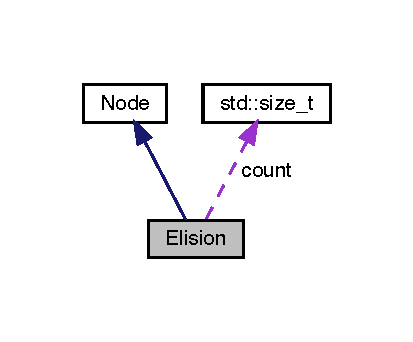
\includegraphics[width=224pt]{struct_elision__coll__graph}
\end{center}
\end{figure}
\subsection*{Public Member Functions}
\begin{DoxyCompactItemize}
\item 
void \hyperlink{struct_elision_ac99f60fccfcedcf9cd090f5682b2e6dd}{accept} (\hyperlink{struct_visitor}{Visitor} \&visitor) const override
\end{DoxyCompactItemize}
\subsection*{Public Attributes}
\begin{DoxyCompactItemize}
\item 
\textbf{ std\+::size\+\_\+t} \hyperlink{struct_elision_a95bc7263a799380ca4e4ddc0cc0eb622}{count} = 1
\end{DoxyCompactItemize}


\subsection{Member Function Documentation}
\mbox{\Hypertarget{struct_elision_ac99f60fccfcedcf9cd090f5682b2e6dd}\label{struct_elision_ac99f60fccfcedcf9cd090f5682b2e6dd}} 
\index{Elision@{Elision}!accept@{accept}}
\index{accept@{accept}!Elision@{Elision}}
\subsubsection{\texorpdfstring{accept()}{accept()}}
{\footnotesize\ttfamily void Elision\+::accept (\begin{DoxyParamCaption}\item[{\hyperlink{struct_visitor}{Visitor} \&}]{visitor }\end{DoxyParamCaption}) const\hspace{0.3cm}{\ttfamily [inline]}, {\ttfamily [override]}, {\ttfamily [virtual]}}



Implements \hyperlink{struct_node_a10bd7af968140bbf5fa461298a969c71}{Node}.



\subsection{Member Data Documentation}
\mbox{\Hypertarget{struct_elision_a95bc7263a799380ca4e4ddc0cc0eb622}\label{struct_elision_a95bc7263a799380ca4e4ddc0cc0eb622}} 
\index{Elision@{Elision}!count@{count}}
\index{count@{count}!Elision@{Elision}}
\subsubsection{\texorpdfstring{count}{count}}
{\footnotesize\ttfamily \textbf{ std\+::size\+\_\+t} Elision\+::count = 1}



The documentation for this struct was generated from the following file\+:\begin{DoxyCompactItemize}
\item 
src/\hyperlink{ast_8h}{ast.\+h}\end{DoxyCompactItemize}

\hypertarget{struct_empty_statement}{}\section{Empty\+Statement Struct Reference}
\label{struct_empty_statement}\index{Empty\+Statement@{Empty\+Statement}}


{\ttfamily \#include $<$ast.\+h$>$}



Inheritance diagram for Empty\+Statement\+:\nopagebreak
\begin{figure}[H]
\begin{center}
\leavevmode
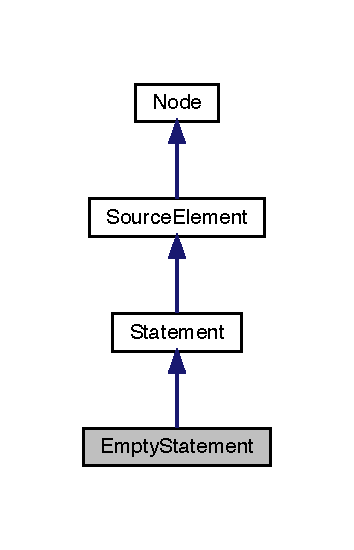
\includegraphics[width=170pt]{struct_empty_statement__inherit__graph}
\end{center}
\end{figure}


Collaboration diagram for Empty\+Statement\+:\nopagebreak
\begin{figure}[H]
\begin{center}
\leavevmode
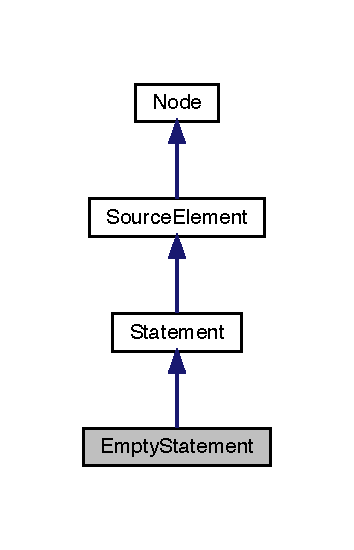
\includegraphics[width=170pt]{struct_empty_statement__coll__graph}
\end{center}
\end{figure}
\subsection*{Public Member Functions}
\begin{DoxyCompactItemize}
\item 
void \hyperlink{struct_empty_statement_af0d920224b9b982402a3a72030d49eed}{accept} (\hyperlink{struct_visitor}{Visitor} \&visitor) const override
\item 
const char $\ast$ \hyperlink{struct_empty_statement_a0401a2753b5502b252898a99a714d261}{type} () const override
\end{DoxyCompactItemize}


\subsection{Member Function Documentation}
\mbox{\Hypertarget{struct_empty_statement_af0d920224b9b982402a3a72030d49eed}\label{struct_empty_statement_af0d920224b9b982402a3a72030d49eed}} 
\index{Empty\+Statement@{Empty\+Statement}!accept@{accept}}
\index{accept@{accept}!Empty\+Statement@{Empty\+Statement}}
\subsubsection{\texorpdfstring{accept()}{accept()}}
{\footnotesize\ttfamily void Empty\+Statement\+::accept (\begin{DoxyParamCaption}\item[{\hyperlink{struct_visitor}{Visitor} \&}]{visitor }\end{DoxyParamCaption}) const\hspace{0.3cm}{\ttfamily [inline]}, {\ttfamily [override]}, {\ttfamily [virtual]}}



Implements \hyperlink{struct_node_a10bd7af968140bbf5fa461298a969c71}{Node}.

\mbox{\Hypertarget{struct_empty_statement_a0401a2753b5502b252898a99a714d261}\label{struct_empty_statement_a0401a2753b5502b252898a99a714d261}} 
\index{Empty\+Statement@{Empty\+Statement}!type@{type}}
\index{type@{type}!Empty\+Statement@{Empty\+Statement}}
\subsubsection{\texorpdfstring{type()}{type()}}
{\footnotesize\ttfamily const char$\ast$ Empty\+Statement\+::type (\begin{DoxyParamCaption}{ }\end{DoxyParamCaption}) const\hspace{0.3cm}{\ttfamily [inline]}, {\ttfamily [override]}, {\ttfamily [virtual]}}



Implements \hyperlink{struct_node_a82f29420d0a38efcc370352528e94e9b}{Node}.



The documentation for this struct was generated from the following file\+:\begin{DoxyCompactItemize}
\item 
src/\hyperlink{ast_8h}{ast.\+h}\end{DoxyCompactItemize}

\hypertarget{class_eval_visitor}{}\section{Eval\+Visitor Class Reference}
\label{class_eval_visitor}\index{Eval\+Visitor@{Eval\+Visitor}}


{\ttfamily \#include $<$eval\+\_\+visitor.\+h$>$}



Inheritance diagram for Eval\+Visitor\+:
\nopagebreak
\begin{figure}[H]
\begin{center}
\leavevmode
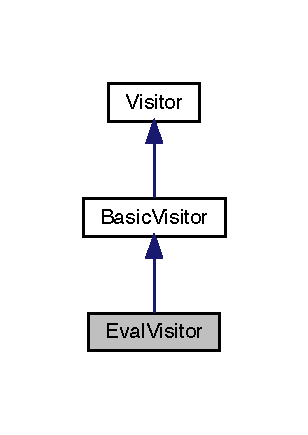
\includegraphics[width=148pt]{class_eval_visitor__inherit__graph}
\end{center}
\end{figure}


Collaboration diagram for Eval\+Visitor\+:
\nopagebreak
\begin{figure}[H]
\begin{center}
\leavevmode
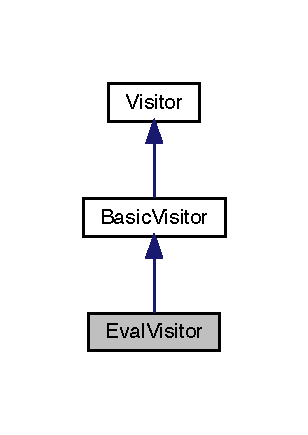
\includegraphics[width=148pt]{class_eval_visitor__coll__graph}
\end{center}
\end{figure}
\subsection*{Public Member Functions}
\begin{DoxyCompactItemize}
\item 
\textbf{ std\+::string} \hyperlink{class_eval_visitor_a999cfe6d55d85b27a6dca7c5f8c2b07e}{str} () const
\item 
void \hyperlink{class_eval_visitor_a9300ec33c193788bec2484b0d99c7fa3}{operator()} (const \hyperlink{struct_program}{Program} \&program) override
\item 
void \hyperlink{class_eval_visitor_a7122ac9fb6f1ef01696296b6bd2edbeb}{operator()} (const \hyperlink{struct_expression_statement}{Expression\+Statement} \&stmt) override
\end{DoxyCompactItemize}


\subsection{Member Function Documentation}
\mbox{\Hypertarget{class_eval_visitor_a9300ec33c193788bec2484b0d99c7fa3}\label{class_eval_visitor_a9300ec33c193788bec2484b0d99c7fa3}} 
\index{Eval\+Visitor@{Eval\+Visitor}!operator()@{operator()}}
\index{operator()@{operator()}!Eval\+Visitor@{Eval\+Visitor}}
\subsubsection{\texorpdfstring{operator()()}{operator()()}\hspace{0.1cm}{\footnotesize\ttfamily [1/2]}}
{\footnotesize\ttfamily void Eval\+Visitor\+::operator() (\begin{DoxyParamCaption}\item[{const \hyperlink{struct_program}{Program} \&}]{program }\end{DoxyParamCaption})\hspace{0.3cm}{\ttfamily [inline]}, {\ttfamily [override]}, {\ttfamily [virtual]}}



Reimplemented from \hyperlink{struct_basic_visitor_adeaf13cc53c36c871d89d6f42a1ec8db}{Basic\+Visitor}.

\mbox{\Hypertarget{class_eval_visitor_a7122ac9fb6f1ef01696296b6bd2edbeb}\label{class_eval_visitor_a7122ac9fb6f1ef01696296b6bd2edbeb}} 
\index{Eval\+Visitor@{Eval\+Visitor}!operator()@{operator()}}
\index{operator()@{operator()}!Eval\+Visitor@{Eval\+Visitor}}
\subsubsection{\texorpdfstring{operator()()}{operator()()}\hspace{0.1cm}{\footnotesize\ttfamily [2/2]}}
{\footnotesize\ttfamily void Eval\+Visitor\+::operator() (\begin{DoxyParamCaption}\item[{const \hyperlink{struct_expression_statement}{Expression\+Statement} \&}]{stmt }\end{DoxyParamCaption})\hspace{0.3cm}{\ttfamily [inline]}, {\ttfamily [override]}, {\ttfamily [virtual]}}



Reimplemented from \hyperlink{struct_basic_visitor_a6c369f60a28dffd5149258e32a81cb6e}{Basic\+Visitor}.

\mbox{\Hypertarget{class_eval_visitor_a999cfe6d55d85b27a6dca7c5f8c2b07e}\label{class_eval_visitor_a999cfe6d55d85b27a6dca7c5f8c2b07e}} 
\index{Eval\+Visitor@{Eval\+Visitor}!str@{str}}
\index{str@{str}!Eval\+Visitor@{Eval\+Visitor}}
\subsubsection{\texorpdfstring{str()}{str()}}
{\footnotesize\ttfamily \textbf{ std\+::string} Eval\+Visitor\+::str (\begin{DoxyParamCaption}{ }\end{DoxyParamCaption}) const\hspace{0.3cm}{\ttfamily [inline]}}



The documentation for this class was generated from the following file\+:\begin{DoxyCompactItemize}
\item 
src/\hyperlink{eval__visitor_8h}{eval\+\_\+visitor.\+h}\end{DoxyCompactItemize}

\hypertarget{struct_expression}{}\section{Expression Struct Reference}
\label{struct_expression}\index{Expression@{Expression}}


{\ttfamily \#include $<$ast.\+h$>$}



Inheritance diagram for Expression\+:\nopagebreak
\begin{figure}[H]
\begin{center}
\leavevmode
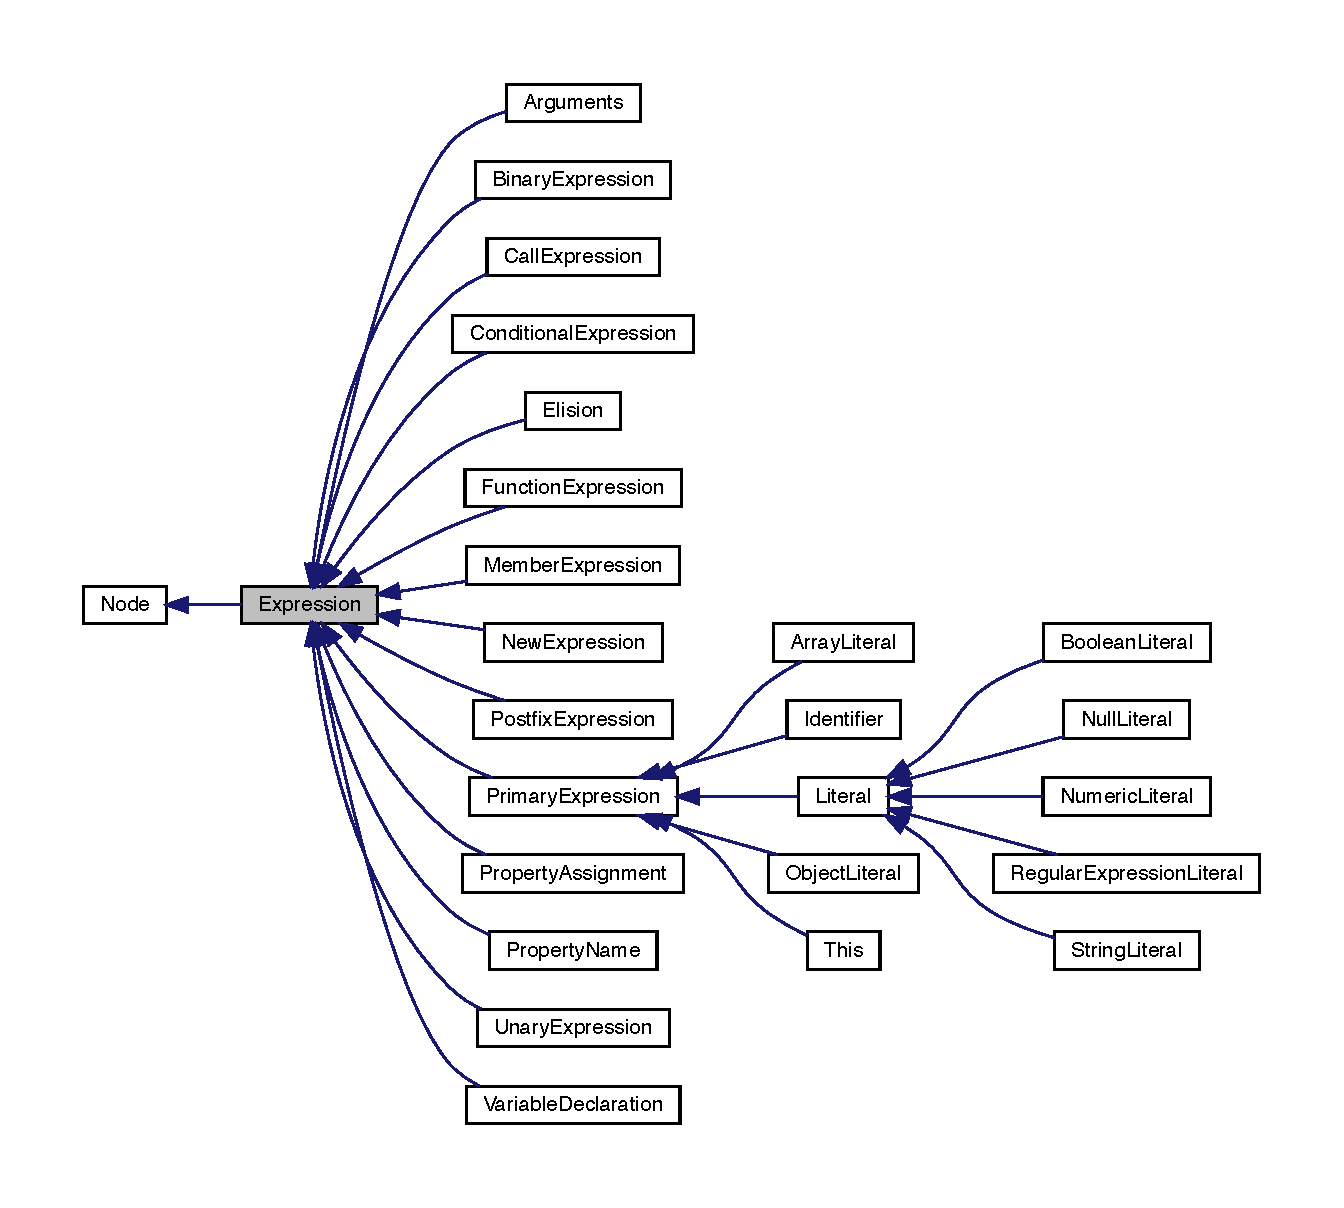
\includegraphics[width=350pt]{struct_expression__inherit__graph}
\end{center}
\end{figure}


Collaboration diagram for Expression\+:\nopagebreak
\begin{figure}[H]
\begin{center}
\leavevmode
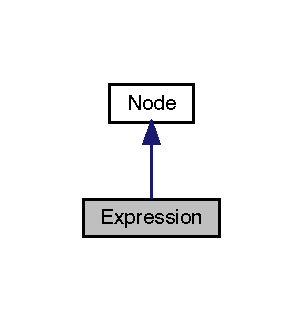
\includegraphics[width=145pt]{struct_expression__coll__graph}
\end{center}
\end{figure}
\subsection*{Additional Inherited Members}


The documentation for this struct was generated from the following file\+:\begin{DoxyCompactItemize}
\item 
src/\hyperlink{ast_8h}{ast.\+h}\end{DoxyCompactItemize}

\hypertarget{struct_expression_statement}{}\section{Expression\+Statement Struct Reference}
\label{struct_expression_statement}\index{Expression\+Statement@{Expression\+Statement}}


{\ttfamily \#include $<$ast.\+h$>$}



Inheritance diagram for Expression\+Statement\+:
\nopagebreak
\begin{figure}[H]
\begin{center}
\leavevmode
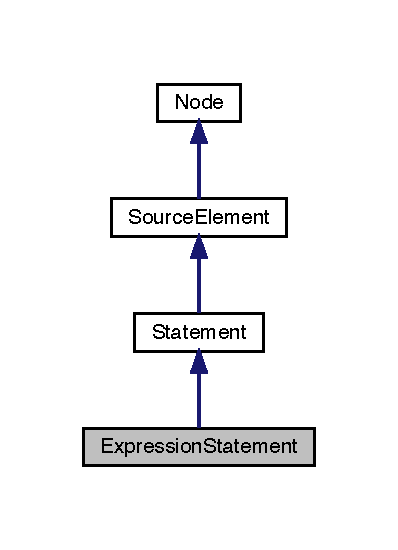
\includegraphics[width=191pt]{struct_expression_statement__inherit__graph}
\end{center}
\end{figure}


Collaboration diagram for Expression\+Statement\+:
\nopagebreak
\begin{figure}[H]
\begin{center}
\leavevmode
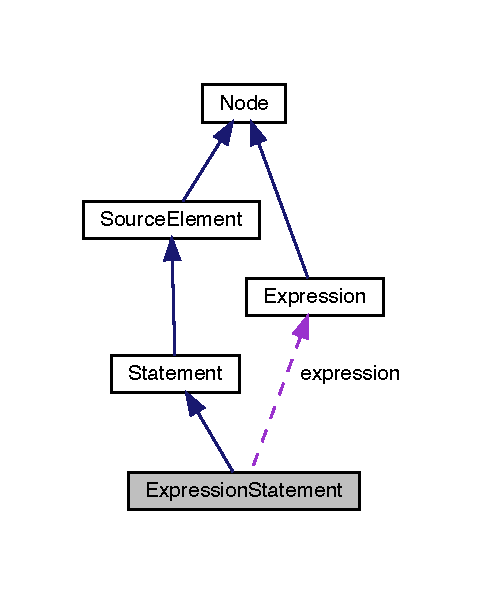
\includegraphics[width=232pt]{struct_expression_statement__coll__graph}
\end{center}
\end{figure}
\subsection*{Public Member Functions}
\begin{DoxyCompactItemize}
\item 
\hyperlink{struct_expression_statement_ad195f09357c26895bf7b8ac7e30ddde3}{Expression\+Statement} (\hyperlink{struct_expression}{Expression} $\ast$\hyperlink{struct_expression_statement_af8fa751297f7dd719ebe74d62201fc3a}{expression})
\item 
void \hyperlink{struct_expression_statement_a6463f779ec4140b2510d854726aefd40}{accept} (\hyperlink{struct_visitor}{Visitor} \&visitor) const override
\end{DoxyCompactItemize}
\subsection*{Public Attributes}
\begin{DoxyCompactItemize}
\item 
\hyperlink{struct_expression}{Expression} $\ast$ \hyperlink{struct_expression_statement_af8fa751297f7dd719ebe74d62201fc3a}{expression}
\end{DoxyCompactItemize}


\subsection{Constructor \& Destructor Documentation}
\mbox{\Hypertarget{struct_expression_statement_ad195f09357c26895bf7b8ac7e30ddde3}\label{struct_expression_statement_ad195f09357c26895bf7b8ac7e30ddde3}} 
\index{Expression\+Statement@{Expression\+Statement}!Expression\+Statement@{Expression\+Statement}}
\index{Expression\+Statement@{Expression\+Statement}!Expression\+Statement@{Expression\+Statement}}
\subsubsection{\texorpdfstring{Expression\+Statement()}{ExpressionStatement()}}
{\footnotesize\ttfamily Expression\+Statement\+::\+Expression\+Statement (\begin{DoxyParamCaption}\item[{\hyperlink{struct_expression}{Expression} $\ast$}]{expression }\end{DoxyParamCaption})\hspace{0.3cm}{\ttfamily [inline]}}



\subsection{Member Function Documentation}
\mbox{\Hypertarget{struct_expression_statement_a6463f779ec4140b2510d854726aefd40}\label{struct_expression_statement_a6463f779ec4140b2510d854726aefd40}} 
\index{Expression\+Statement@{Expression\+Statement}!accept@{accept}}
\index{accept@{accept}!Expression\+Statement@{Expression\+Statement}}
\subsubsection{\texorpdfstring{accept()}{accept()}}
{\footnotesize\ttfamily void Expression\+Statement\+::accept (\begin{DoxyParamCaption}\item[{\hyperlink{struct_visitor}{Visitor} \&}]{visitor }\end{DoxyParamCaption}) const\hspace{0.3cm}{\ttfamily [inline]}, {\ttfamily [override]}, {\ttfamily [virtual]}}



Implements \hyperlink{struct_node_a10bd7af968140bbf5fa461298a969c71}{Node}.



\subsection{Member Data Documentation}
\mbox{\Hypertarget{struct_expression_statement_af8fa751297f7dd719ebe74d62201fc3a}\label{struct_expression_statement_af8fa751297f7dd719ebe74d62201fc3a}} 
\index{Expression\+Statement@{Expression\+Statement}!expression@{expression}}
\index{expression@{expression}!Expression\+Statement@{Expression\+Statement}}
\subsubsection{\texorpdfstring{expression}{expression}}
{\footnotesize\ttfamily \hyperlink{struct_expression}{Expression}$\ast$ Expression\+Statement\+::expression}



The documentation for this struct was generated from the following file\+:\begin{DoxyCompactItemize}
\item 
src/\hyperlink{ast_8h}{ast.\+h}\end{DoxyCompactItemize}

\hypertarget{struct_for_in_statement}{}\section{For\+In\+Statement Struct Reference}
\label{struct_for_in_statement}\index{For\+In\+Statement@{For\+In\+Statement}}


{\ttfamily \#include $<$ast.\+h$>$}



Inheritance diagram for For\+In\+Statement\+:\nopagebreak
\begin{figure}[H]
\begin{center}
\leavevmode
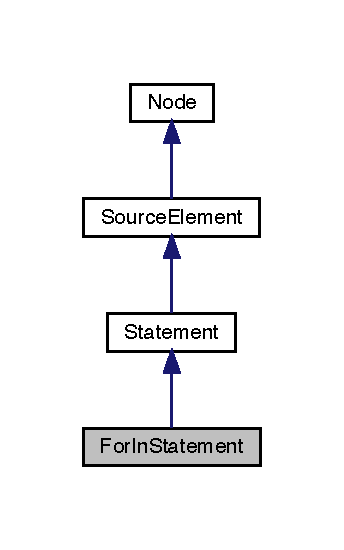
\includegraphics[width=165pt]{struct_for_in_statement__inherit__graph}
\end{center}
\end{figure}


Collaboration diagram for For\+In\+Statement\+:
\nopagebreak
\begin{figure}[H]
\begin{center}
\leavevmode
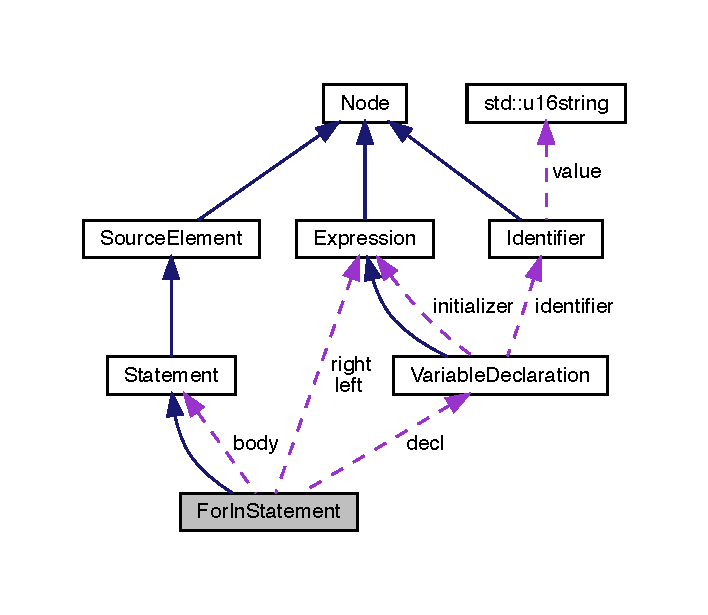
\includegraphics[width=225pt]{struct_for_in_statement__coll__graph}
\end{center}
\end{figure}
\subsection*{Public Member Functions}
\begin{DoxyCompactItemize}
\item 
\hyperlink{struct_for_in_statement_aa3565db4851cca290147f4d98b275c68}{For\+In\+Statement} (\hyperlink{struct_left_hand_side_expression}{Left\+Hand\+Side\+Expression} $\ast$\hyperlink{struct_for_in_statement_acb865c777a9c3ccbe84ed09532f1a22f}{left}, \hyperlink{struct_expression}{Expression} $\ast$\hyperlink{struct_for_in_statement_a8aec27cbc19e2cb038acd3d0fc0a1969}{right}=nullptr, \hyperlink{struct_statement}{Statement} $\ast$\hyperlink{struct_for_in_statement_a865933063222b4eb53866423c444c1ca}{body}=nullptr)
\item 
\hyperlink{struct_for_in_statement_aa78680c185913cd46be68a67cbe43b27}{For\+In\+Statement} (\hyperlink{struct_variable_declaration}{Variable\+Declaration} $\ast$\hyperlink{struct_for_in_statement_acb865c777a9c3ccbe84ed09532f1a22f}{left}, \hyperlink{struct_expression}{Expression} $\ast$\hyperlink{struct_for_in_statement_a8aec27cbc19e2cb038acd3d0fc0a1969}{right}=nullptr, \hyperlink{struct_statement}{Statement} $\ast$\hyperlink{struct_for_in_statement_a865933063222b4eb53866423c444c1ca}{body}=nullptr)
\item 
void \hyperlink{struct_for_in_statement_ab5ee623aba6eebd12e52a9196e33e64b}{accept} (\hyperlink{struct_visitor}{Visitor} \&visitor) const override
\item 
const char $\ast$ \hyperlink{struct_for_in_statement_a5dd65175f49087b46e5e2f6d34246a1f}{type} () const override
\end{DoxyCompactItemize}
\subsection*{Public Attributes}
\begin{DoxyCompactItemize}
\item 
\hyperlink{struct_expression}{Expression} $\ast$ \hyperlink{struct_for_in_statement_acb865c777a9c3ccbe84ed09532f1a22f}{left}
\item 
\hyperlink{struct_expression}{Expression} $\ast$ \hyperlink{struct_for_in_statement_a8aec27cbc19e2cb038acd3d0fc0a1969}{right}
\item 
\hyperlink{struct_statement}{Statement} $\ast$ \hyperlink{struct_for_in_statement_a865933063222b4eb53866423c444c1ca}{body}
\end{DoxyCompactItemize}


\subsection{Constructor \& Destructor Documentation}
\mbox{\Hypertarget{struct_for_in_statement_aa3565db4851cca290147f4d98b275c68}\label{struct_for_in_statement_aa3565db4851cca290147f4d98b275c68}} 
\index{For\+In\+Statement@{For\+In\+Statement}!For\+In\+Statement@{For\+In\+Statement}}
\index{For\+In\+Statement@{For\+In\+Statement}!For\+In\+Statement@{For\+In\+Statement}}
\subsubsection{\texorpdfstring{For\+In\+Statement()}{ForInStatement()}\hspace{0.1cm}{\footnotesize\ttfamily [1/2]}}
{\footnotesize\ttfamily For\+In\+Statement\+::\+For\+In\+Statement (\begin{DoxyParamCaption}\item[{\hyperlink{struct_left_hand_side_expression}{Left\+Hand\+Side\+Expression} $\ast$}]{left,  }\item[{\hyperlink{struct_expression}{Expression} $\ast$}]{right = {\ttfamily nullptr},  }\item[{\hyperlink{struct_statement}{Statement} $\ast$}]{body = {\ttfamily nullptr} }\end{DoxyParamCaption})\hspace{0.3cm}{\ttfamily [inline]}}

\mbox{\Hypertarget{struct_for_in_statement_aa78680c185913cd46be68a67cbe43b27}\label{struct_for_in_statement_aa78680c185913cd46be68a67cbe43b27}} 
\index{For\+In\+Statement@{For\+In\+Statement}!For\+In\+Statement@{For\+In\+Statement}}
\index{For\+In\+Statement@{For\+In\+Statement}!For\+In\+Statement@{For\+In\+Statement}}
\subsubsection{\texorpdfstring{For\+In\+Statement()}{ForInStatement()}\hspace{0.1cm}{\footnotesize\ttfamily [2/2]}}
{\footnotesize\ttfamily For\+In\+Statement\+::\+For\+In\+Statement (\begin{DoxyParamCaption}\item[{\hyperlink{struct_variable_declaration}{Variable\+Declaration} $\ast$}]{left,  }\item[{\hyperlink{struct_expression}{Expression} $\ast$}]{right = {\ttfamily nullptr},  }\item[{\hyperlink{struct_statement}{Statement} $\ast$}]{body = {\ttfamily nullptr} }\end{DoxyParamCaption})\hspace{0.3cm}{\ttfamily [inline]}}



\subsection{Member Function Documentation}
\mbox{\Hypertarget{struct_for_in_statement_ab5ee623aba6eebd12e52a9196e33e64b}\label{struct_for_in_statement_ab5ee623aba6eebd12e52a9196e33e64b}} 
\index{For\+In\+Statement@{For\+In\+Statement}!accept@{accept}}
\index{accept@{accept}!For\+In\+Statement@{For\+In\+Statement}}
\subsubsection{\texorpdfstring{accept()}{accept()}}
{\footnotesize\ttfamily void For\+In\+Statement\+::accept (\begin{DoxyParamCaption}\item[{\hyperlink{struct_visitor}{Visitor} \&}]{visitor }\end{DoxyParamCaption}) const\hspace{0.3cm}{\ttfamily [inline]}, {\ttfamily [override]}, {\ttfamily [virtual]}}



Implements \hyperlink{struct_node_a10bd7af968140bbf5fa461298a969c71}{Node}.

\mbox{\Hypertarget{struct_for_in_statement_a5dd65175f49087b46e5e2f6d34246a1f}\label{struct_for_in_statement_a5dd65175f49087b46e5e2f6d34246a1f}} 
\index{For\+In\+Statement@{For\+In\+Statement}!type@{type}}
\index{type@{type}!For\+In\+Statement@{For\+In\+Statement}}
\subsubsection{\texorpdfstring{type()}{type()}}
{\footnotesize\ttfamily const char$\ast$ For\+In\+Statement\+::type (\begin{DoxyParamCaption}{ }\end{DoxyParamCaption}) const\hspace{0.3cm}{\ttfamily [inline]}, {\ttfamily [override]}, {\ttfamily [virtual]}}



Implements \hyperlink{struct_node_a82f29420d0a38efcc370352528e94e9b}{Node}.



\subsection{Member Data Documentation}
\mbox{\Hypertarget{struct_for_in_statement_a865933063222b4eb53866423c444c1ca}\label{struct_for_in_statement_a865933063222b4eb53866423c444c1ca}} 
\index{For\+In\+Statement@{For\+In\+Statement}!body@{body}}
\index{body@{body}!For\+In\+Statement@{For\+In\+Statement}}
\subsubsection{\texorpdfstring{body}{body}}
{\footnotesize\ttfamily \hyperlink{struct_statement}{Statement}$\ast$ For\+In\+Statement\+::body}

\mbox{\Hypertarget{struct_for_in_statement_acb865c777a9c3ccbe84ed09532f1a22f}\label{struct_for_in_statement_acb865c777a9c3ccbe84ed09532f1a22f}} 
\index{For\+In\+Statement@{For\+In\+Statement}!left@{left}}
\index{left@{left}!For\+In\+Statement@{For\+In\+Statement}}
\subsubsection{\texorpdfstring{left}{left}}
{\footnotesize\ttfamily \hyperlink{struct_expression}{Expression}$\ast$ For\+In\+Statement\+::left}

\mbox{\Hypertarget{struct_for_in_statement_a8aec27cbc19e2cb038acd3d0fc0a1969}\label{struct_for_in_statement_a8aec27cbc19e2cb038acd3d0fc0a1969}} 
\index{For\+In\+Statement@{For\+In\+Statement}!right@{right}}
\index{right@{right}!For\+In\+Statement@{For\+In\+Statement}}
\subsubsection{\texorpdfstring{right}{right}}
{\footnotesize\ttfamily \hyperlink{struct_expression}{Expression}$\ast$ For\+In\+Statement\+::right}



The documentation for this struct was generated from the following file\+:\begin{DoxyCompactItemize}
\item 
src/\hyperlink{ast_8h}{ast.\+h}\end{DoxyCompactItemize}

\hypertarget{struct_formal_parameter_list}{}\section{Formal\+Parameter\+List Struct Reference}
\label{struct_formal_parameter_list}\index{Formal\+Parameter\+List@{Formal\+Parameter\+List}}


{\ttfamily \#include $<$ast.\+h$>$}



Inheritance diagram for Formal\+Parameter\+List\+:\nopagebreak
\begin{figure}[H]
\begin{center}
\leavevmode
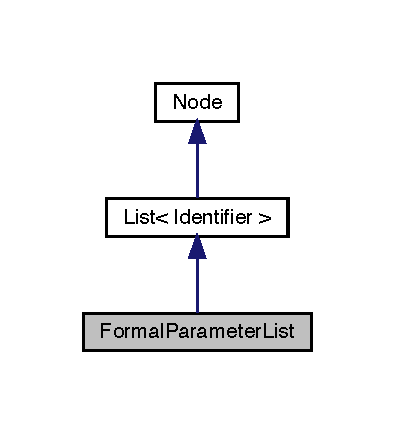
\includegraphics[width=189pt]{struct_formal_parameter_list__inherit__graph}
\end{center}
\end{figure}


Collaboration diagram for Formal\+Parameter\+List\+:\nopagebreak
\begin{figure}[H]
\begin{center}
\leavevmode
\includegraphics[width=260pt]{struct_formal_parameter_list__coll__graph}
\end{center}
\end{figure}
\subsection*{Additional Inherited Members}


The documentation for this struct was generated from the following file\+:\begin{DoxyCompactItemize}
\item 
src/\hyperlink{ast_8h}{ast.\+h}\end{DoxyCompactItemize}

\hypertarget{struct_for_statement}{}\section{For\+Statement Struct Reference}
\label{struct_for_statement}\index{For\+Statement@{For\+Statement}}


{\ttfamily \#include $<$ast.\+h$>$}



Inheritance diagram for For\+Statement\+:\nopagebreak
\begin{figure}[H]
\begin{center}
\leavevmode
\includegraphics[width=164pt]{struct_for_statement__inherit__graph}
\end{center}
\end{figure}


Collaboration diagram for For\+Statement\+:\nopagebreak
\begin{figure}[H]
\begin{center}
\leavevmode
\includegraphics[width=238pt]{struct_for_statement__coll__graph}
\end{center}
\end{figure}
\subsection*{Public Member Functions}
\begin{DoxyCompactItemize}
\item 
\hyperlink{struct_for_statement_ac6f0bfa1c5a48bcf2ed048639e13cd16}{For\+Statement} (\hyperlink{struct_variable_declaration_list}{Variable\+Declaration\+List} $\ast$\hyperlink{struct_for_statement_aa4516b04bff706f5ad80915357da05e5}{init}, \hyperlink{struct_expression}{Expression} $\ast$\hyperlink{struct_for_statement_a97f163e3d73072eccf4b86120ee17efb}{test}=nullptr, \hyperlink{struct_expression}{Expression} $\ast$\hyperlink{struct_for_statement_ae0e9d64880b5db76426fdb453275fd90}{update}=nullptr, \hyperlink{struct_statement}{Statement} $\ast$\hyperlink{struct_for_statement_a8d9018f1d05bcd027122c9dcabb0e3ba}{body}=nullptr)
\item 
\hyperlink{struct_for_statement_a3073886e1dc3db4bd301331596da922b}{For\+Statement} (\hyperlink{struct_expression}{Expression} $\ast$\hyperlink{struct_for_statement_aa4516b04bff706f5ad80915357da05e5}{init}=nullptr, \hyperlink{struct_expression}{Expression} $\ast$\hyperlink{struct_for_statement_a97f163e3d73072eccf4b86120ee17efb}{test}=nullptr, \hyperlink{struct_expression}{Expression} $\ast$\hyperlink{struct_for_statement_ae0e9d64880b5db76426fdb453275fd90}{update}=nullptr, \hyperlink{struct_statement}{Statement} $\ast$\hyperlink{struct_for_statement_a8d9018f1d05bcd027122c9dcabb0e3ba}{body}=nullptr)
\item 
void \hyperlink{struct_for_statement_acc3a0ac5de61092f0d7be7921b31d47d}{accept} (\hyperlink{struct_visitor}{Visitor} \&visitor) const override
\item 
const char $\ast$ \hyperlink{struct_for_statement_acf0f64ddd1a41763f15af08813b0bea6}{type} () const override
\end{DoxyCompactItemize}
\subsection*{Public Attributes}
\begin{DoxyCompactItemize}
\item 
\hyperlink{struct_node}{Node} $\ast$ \hyperlink{struct_for_statement_aa4516b04bff706f5ad80915357da05e5}{init}
\item 
\hyperlink{struct_expression}{Expression} $\ast$ \hyperlink{struct_for_statement_a97f163e3d73072eccf4b86120ee17efb}{test}
\item 
\hyperlink{struct_expression}{Expression} $\ast$ \hyperlink{struct_for_statement_ae0e9d64880b5db76426fdb453275fd90}{update}
\item 
\hyperlink{struct_statement}{Statement} $\ast$ \hyperlink{struct_for_statement_a8d9018f1d05bcd027122c9dcabb0e3ba}{body}
\end{DoxyCompactItemize}


\subsection{Constructor \& Destructor Documentation}
\mbox{\Hypertarget{struct_for_statement_ac6f0bfa1c5a48bcf2ed048639e13cd16}\label{struct_for_statement_ac6f0bfa1c5a48bcf2ed048639e13cd16}} 
\index{For\+Statement@{For\+Statement}!For\+Statement@{For\+Statement}}
\index{For\+Statement@{For\+Statement}!For\+Statement@{For\+Statement}}
\subsubsection{\texorpdfstring{For\+Statement()}{ForStatement()}\hspace{0.1cm}{\footnotesize\ttfamily [1/2]}}
{\footnotesize\ttfamily For\+Statement\+::\+For\+Statement (\begin{DoxyParamCaption}\item[{\hyperlink{struct_variable_declaration_list}{Variable\+Declaration\+List} $\ast$}]{init,  }\item[{\hyperlink{struct_expression}{Expression} $\ast$}]{test = {\ttfamily nullptr},  }\item[{\hyperlink{struct_expression}{Expression} $\ast$}]{update = {\ttfamily nullptr},  }\item[{\hyperlink{struct_statement}{Statement} $\ast$}]{body = {\ttfamily nullptr} }\end{DoxyParamCaption})\hspace{0.3cm}{\ttfamily [inline]}}

\mbox{\Hypertarget{struct_for_statement_a3073886e1dc3db4bd301331596da922b}\label{struct_for_statement_a3073886e1dc3db4bd301331596da922b}} 
\index{For\+Statement@{For\+Statement}!For\+Statement@{For\+Statement}}
\index{For\+Statement@{For\+Statement}!For\+Statement@{For\+Statement}}
\subsubsection{\texorpdfstring{For\+Statement()}{ForStatement()}\hspace{0.1cm}{\footnotesize\ttfamily [2/2]}}
{\footnotesize\ttfamily For\+Statement\+::\+For\+Statement (\begin{DoxyParamCaption}\item[{\hyperlink{struct_expression}{Expression} $\ast$}]{init = {\ttfamily nullptr},  }\item[{\hyperlink{struct_expression}{Expression} $\ast$}]{test = {\ttfamily nullptr},  }\item[{\hyperlink{struct_expression}{Expression} $\ast$}]{update = {\ttfamily nullptr},  }\item[{\hyperlink{struct_statement}{Statement} $\ast$}]{body = {\ttfamily nullptr} }\end{DoxyParamCaption})\hspace{0.3cm}{\ttfamily [inline]}}



\subsection{Member Function Documentation}
\mbox{\Hypertarget{struct_for_statement_acc3a0ac5de61092f0d7be7921b31d47d}\label{struct_for_statement_acc3a0ac5de61092f0d7be7921b31d47d}} 
\index{For\+Statement@{For\+Statement}!accept@{accept}}
\index{accept@{accept}!For\+Statement@{For\+Statement}}
\subsubsection{\texorpdfstring{accept()}{accept()}}
{\footnotesize\ttfamily void For\+Statement\+::accept (\begin{DoxyParamCaption}\item[{\hyperlink{struct_visitor}{Visitor} \&}]{visitor }\end{DoxyParamCaption}) const\hspace{0.3cm}{\ttfamily [inline]}, {\ttfamily [override]}, {\ttfamily [virtual]}}



Implements \hyperlink{struct_node_a10bd7af968140bbf5fa461298a969c71}{Node}.

\mbox{\Hypertarget{struct_for_statement_acf0f64ddd1a41763f15af08813b0bea6}\label{struct_for_statement_acf0f64ddd1a41763f15af08813b0bea6}} 
\index{For\+Statement@{For\+Statement}!type@{type}}
\index{type@{type}!For\+Statement@{For\+Statement}}
\subsubsection{\texorpdfstring{type()}{type()}}
{\footnotesize\ttfamily const char$\ast$ For\+Statement\+::type (\begin{DoxyParamCaption}{ }\end{DoxyParamCaption}) const\hspace{0.3cm}{\ttfamily [inline]}, {\ttfamily [override]}, {\ttfamily [virtual]}}



Implements \hyperlink{struct_node_a82f29420d0a38efcc370352528e94e9b}{Node}.



\subsection{Member Data Documentation}
\mbox{\Hypertarget{struct_for_statement_a8d9018f1d05bcd027122c9dcabb0e3ba}\label{struct_for_statement_a8d9018f1d05bcd027122c9dcabb0e3ba}} 
\index{For\+Statement@{For\+Statement}!body@{body}}
\index{body@{body}!For\+Statement@{For\+Statement}}
\subsubsection{\texorpdfstring{body}{body}}
{\footnotesize\ttfamily \hyperlink{struct_statement}{Statement}$\ast$ For\+Statement\+::body}

\mbox{\Hypertarget{struct_for_statement_aa4516b04bff706f5ad80915357da05e5}\label{struct_for_statement_aa4516b04bff706f5ad80915357da05e5}} 
\index{For\+Statement@{For\+Statement}!init@{init}}
\index{init@{init}!For\+Statement@{For\+Statement}}
\subsubsection{\texorpdfstring{init}{init}}
{\footnotesize\ttfamily \hyperlink{struct_node}{Node}$\ast$ For\+Statement\+::init}

\mbox{\Hypertarget{struct_for_statement_a97f163e3d73072eccf4b86120ee17efb}\label{struct_for_statement_a97f163e3d73072eccf4b86120ee17efb}} 
\index{For\+Statement@{For\+Statement}!test@{test}}
\index{test@{test}!For\+Statement@{For\+Statement}}
\subsubsection{\texorpdfstring{test}{test}}
{\footnotesize\ttfamily \hyperlink{struct_expression}{Expression}$\ast$ For\+Statement\+::test}

\mbox{\Hypertarget{struct_for_statement_ae0e9d64880b5db76426fdb453275fd90}\label{struct_for_statement_ae0e9d64880b5db76426fdb453275fd90}} 
\index{For\+Statement@{For\+Statement}!update@{update}}
\index{update@{update}!For\+Statement@{For\+Statement}}
\subsubsection{\texorpdfstring{update}{update}}
{\footnotesize\ttfamily \hyperlink{struct_expression}{Expression}$\ast$ For\+Statement\+::update}



The documentation for this struct was generated from the following file\+:\begin{DoxyCompactItemize}
\item 
src/\hyperlink{ast_8h}{ast.\+h}\end{DoxyCompactItemize}

\hypertarget{struct_function_body}{}\section{Function\+Body Struct Reference}
\label{struct_function_body}\index{Function\+Body@{Function\+Body}}


{\ttfamily \#include $<$ast.\+h$>$}



Inheritance diagram for Function\+Body\+:
\nopagebreak
\begin{figure}[H]
\begin{center}
\leavevmode
\includegraphics[width=197pt]{struct_function_body__inherit__graph}
\end{center}
\end{figure}


Collaboration diagram for Function\+Body\+:
\nopagebreak
\begin{figure}[H]
\begin{center}
\leavevmode
\includegraphics[width=290pt]{struct_function_body__coll__graph}
\end{center}
\end{figure}
\subsection*{Public Member Functions}
\begin{DoxyCompactItemize}
\item 
\hyperlink{struct_function_body_a0ba6abdbb2090c64d9892d4064234865}{Function\+Body} (\hyperlink{struct_source_elements}{Source\+Elements} $\ast$body=nullptr)
\item 
void \hyperlink{struct_function_body_ab6acc0d3e8a2bf452045ee4adc78aa26}{accept} (\hyperlink{struct_visitor}{Visitor} \&visitor) const override
\end{DoxyCompactItemize}
\subsection*{Additional Inherited Members}


\subsection{Constructor \& Destructor Documentation}
\mbox{\Hypertarget{struct_function_body_a0ba6abdbb2090c64d9892d4064234865}\label{struct_function_body_a0ba6abdbb2090c64d9892d4064234865}} 
\index{Function\+Body@{Function\+Body}!Function\+Body@{Function\+Body}}
\index{Function\+Body@{Function\+Body}!Function\+Body@{Function\+Body}}
\subsubsection{\texorpdfstring{Function\+Body()}{FunctionBody()}}
{\footnotesize\ttfamily Function\+Body\+::\+Function\+Body (\begin{DoxyParamCaption}\item[{\hyperlink{struct_source_elements}{Source\+Elements} $\ast$}]{body = {\ttfamily nullptr} }\end{DoxyParamCaption})\hspace{0.3cm}{\ttfamily [inline]}}



\subsection{Member Function Documentation}
\mbox{\Hypertarget{struct_function_body_ab6acc0d3e8a2bf452045ee4adc78aa26}\label{struct_function_body_ab6acc0d3e8a2bf452045ee4adc78aa26}} 
\index{Function\+Body@{Function\+Body}!accept@{accept}}
\index{accept@{accept}!Function\+Body@{Function\+Body}}
\subsubsection{\texorpdfstring{accept()}{accept()}}
{\footnotesize\ttfamily void Function\+Body\+::accept (\begin{DoxyParamCaption}\item[{\hyperlink{struct_visitor}{Visitor} \&}]{visitor }\end{DoxyParamCaption}) const\hspace{0.3cm}{\ttfamily [inline]}, {\ttfamily [override]}, {\ttfamily [virtual]}}



Implements \hyperlink{struct_node_a10bd7af968140bbf5fa461298a969c71}{Node}.



The documentation for this struct was generated from the following file\+:\begin{DoxyCompactItemize}
\item 
src/\hyperlink{ast_8h}{ast.\+h}\end{DoxyCompactItemize}

\hypertarget{struct_function_declaration}{}\section{Function\+Declaration Struct Reference}
\label{struct_function_declaration}\index{Function\+Declaration@{Function\+Declaration}}


{\ttfamily \#include $<$ast.\+h$>$}



Inheritance diagram for Function\+Declaration\+:\nopagebreak
\begin{figure}[H]
\begin{center}
\leavevmode
\includegraphics[width=185pt]{struct_function_declaration__inherit__graph}
\end{center}
\end{figure}


Collaboration diagram for Function\+Declaration\+:\nopagebreak
\begin{figure}[H]
\begin{center}
\leavevmode
\includegraphics[width=350pt]{struct_function_declaration__coll__graph}
\end{center}
\end{figure}
\subsection*{Public Member Functions}
\begin{DoxyCompactItemize}
\item 
\hyperlink{struct_function_declaration_a2760e02567ddf39823e4a0b9a69898fa}{Function\+Declaration} (\hyperlink{struct_identifier}{Identifier} $\ast$\hyperlink{struct_function_declaration_a58de81497de15b01a5f92632c3e6f354}{id}, \hyperlink{struct_formal_parameter_list}{Formal\+Parameter\+List} $\ast$\hyperlink{struct_function_declaration_ab22f1972d3575c2b95778545d871658b}{params}, \hyperlink{struct_function_body}{Function\+Body} $\ast$\hyperlink{struct_function_declaration_ae35697bf8c8a45e490fa352d77a0c19b}{body})
\item 
void \hyperlink{struct_function_declaration_ada618c9934e5706066e5521afeada149}{accept} (\hyperlink{struct_visitor}{Visitor} \&visitor) const override
\item 
const char $\ast$ \hyperlink{struct_function_declaration_aff2da7f2c794e8ce1c3c7c15e9f88eb7}{type} () const override
\end{DoxyCompactItemize}
\subsection*{Public Attributes}
\begin{DoxyCompactItemize}
\item 
\hyperlink{struct_identifier}{Identifier} $\ast$ \hyperlink{struct_function_declaration_a58de81497de15b01a5f92632c3e6f354}{id}
\item 
\hyperlink{struct_formal_parameter_list}{Formal\+Parameter\+List} $\ast$ \hyperlink{struct_function_declaration_ab22f1972d3575c2b95778545d871658b}{params}
\item 
\hyperlink{struct_function_body}{Function\+Body} $\ast$ \hyperlink{struct_function_declaration_ae35697bf8c8a45e490fa352d77a0c19b}{body}
\end{DoxyCompactItemize}


\subsection{Constructor \& Destructor Documentation}
\mbox{\Hypertarget{struct_function_declaration_a2760e02567ddf39823e4a0b9a69898fa}\label{struct_function_declaration_a2760e02567ddf39823e4a0b9a69898fa}} 
\index{Function\+Declaration@{Function\+Declaration}!Function\+Declaration@{Function\+Declaration}}
\index{Function\+Declaration@{Function\+Declaration}!Function\+Declaration@{Function\+Declaration}}
\subsubsection{\texorpdfstring{Function\+Declaration()}{FunctionDeclaration()}}
{\footnotesize\ttfamily Function\+Declaration\+::\+Function\+Declaration (\begin{DoxyParamCaption}\item[{\hyperlink{struct_identifier}{Identifier} $\ast$}]{id,  }\item[{\hyperlink{struct_formal_parameter_list}{Formal\+Parameter\+List} $\ast$}]{params,  }\item[{\hyperlink{struct_function_body}{Function\+Body} $\ast$}]{body }\end{DoxyParamCaption})\hspace{0.3cm}{\ttfamily [inline]}}



\subsection{Member Function Documentation}
\mbox{\Hypertarget{struct_function_declaration_ada618c9934e5706066e5521afeada149}\label{struct_function_declaration_ada618c9934e5706066e5521afeada149}} 
\index{Function\+Declaration@{Function\+Declaration}!accept@{accept}}
\index{accept@{accept}!Function\+Declaration@{Function\+Declaration}}
\subsubsection{\texorpdfstring{accept()}{accept()}}
{\footnotesize\ttfamily void Function\+Declaration\+::accept (\begin{DoxyParamCaption}\item[{\hyperlink{struct_visitor}{Visitor} \&}]{visitor }\end{DoxyParamCaption}) const\hspace{0.3cm}{\ttfamily [inline]}, {\ttfamily [override]}, {\ttfamily [virtual]}}



Implements \hyperlink{struct_node_a10bd7af968140bbf5fa461298a969c71}{Node}.

\mbox{\Hypertarget{struct_function_declaration_aff2da7f2c794e8ce1c3c7c15e9f88eb7}\label{struct_function_declaration_aff2da7f2c794e8ce1c3c7c15e9f88eb7}} 
\index{Function\+Declaration@{Function\+Declaration}!type@{type}}
\index{type@{type}!Function\+Declaration@{Function\+Declaration}}
\subsubsection{\texorpdfstring{type()}{type()}}
{\footnotesize\ttfamily const char$\ast$ Function\+Declaration\+::type (\begin{DoxyParamCaption}{ }\end{DoxyParamCaption}) const\hspace{0.3cm}{\ttfamily [inline]}, {\ttfamily [override]}, {\ttfamily [virtual]}}



Implements \hyperlink{struct_node_a82f29420d0a38efcc370352528e94e9b}{Node}.



\subsection{Member Data Documentation}
\mbox{\Hypertarget{struct_function_declaration_ae35697bf8c8a45e490fa352d77a0c19b}\label{struct_function_declaration_ae35697bf8c8a45e490fa352d77a0c19b}} 
\index{Function\+Declaration@{Function\+Declaration}!body@{body}}
\index{body@{body}!Function\+Declaration@{Function\+Declaration}}
\subsubsection{\texorpdfstring{body}{body}}
{\footnotesize\ttfamily \hyperlink{struct_function_body}{Function\+Body}$\ast$ Function\+Declaration\+::body}

\mbox{\Hypertarget{struct_function_declaration_a58de81497de15b01a5f92632c3e6f354}\label{struct_function_declaration_a58de81497de15b01a5f92632c3e6f354}} 
\index{Function\+Declaration@{Function\+Declaration}!id@{id}}
\index{id@{id}!Function\+Declaration@{Function\+Declaration}}
\subsubsection{\texorpdfstring{id}{id}}
{\footnotesize\ttfamily \hyperlink{struct_identifier}{Identifier}$\ast$ Function\+Declaration\+::id}

\mbox{\Hypertarget{struct_function_declaration_ab22f1972d3575c2b95778545d871658b}\label{struct_function_declaration_ab22f1972d3575c2b95778545d871658b}} 
\index{Function\+Declaration@{Function\+Declaration}!params@{params}}
\index{params@{params}!Function\+Declaration@{Function\+Declaration}}
\subsubsection{\texorpdfstring{params}{params}}
{\footnotesize\ttfamily \hyperlink{struct_formal_parameter_list}{Formal\+Parameter\+List}$\ast$ Function\+Declaration\+::params}



The documentation for this struct was generated from the following file\+:\begin{DoxyCompactItemize}
\item 
src/\hyperlink{ast_8h}{ast.\+h}\end{DoxyCompactItemize}

\hypertarget{struct_function_expression}{}\section{Function\+Expression Struct Reference}
\label{struct_function_expression}\index{Function\+Expression@{Function\+Expression}}


{\ttfamily \#include $<$ast.\+h$>$}



Collaboration diagram for Function\+Expression\+:\nopagebreak
\begin{figure}[H]
\begin{center}
\leavevmode
\includegraphics[width=328pt]{struct_function_expression__coll__graph}
\end{center}
\end{figure}
\subsection*{Public Attributes}
\begin{DoxyCompactItemize}
\item 
boost\+::optional$<$ \hyperlink{struct_identifier}{Identifier} $>$ \hyperlink{struct_function_expression_a6c7220587de4e7731ff712d6535180c2}{id}
\item 
\hyperlink{ast_8h_ad423d9c7b02512f74f787f74587e9e76}{Formal\+Parameter\+List} \hyperlink{struct_function_expression_adf1fd5d4d8c6fca0d4496dcad8430996}{params}
\item 
\hyperlink{struct_function_body}{Function\+Body} \hyperlink{struct_function_expression_a82a9fa3ab1eb96e69f11f41445e5ad5c}{body}
\end{DoxyCompactItemize}


\subsection{Member Data Documentation}
\mbox{\Hypertarget{struct_function_expression_a82a9fa3ab1eb96e69f11f41445e5ad5c}\label{struct_function_expression_a82a9fa3ab1eb96e69f11f41445e5ad5c}} 
\index{Function\+Expression@{Function\+Expression}!body@{body}}
\index{body@{body}!Function\+Expression@{Function\+Expression}}
\subsubsection{\texorpdfstring{body}{body}}
{\footnotesize\ttfamily \hyperlink{struct_function_body}{Function\+Body} Function\+Expression\+::body}

\mbox{\Hypertarget{struct_function_expression_a6c7220587de4e7731ff712d6535180c2}\label{struct_function_expression_a6c7220587de4e7731ff712d6535180c2}} 
\index{Function\+Expression@{Function\+Expression}!id@{id}}
\index{id@{id}!Function\+Expression@{Function\+Expression}}
\subsubsection{\texorpdfstring{id}{id}}
{\footnotesize\ttfamily boost\+::optional$<$\hyperlink{struct_identifier}{Identifier}$>$ Function\+Expression\+::id}

\mbox{\Hypertarget{struct_function_expression_adf1fd5d4d8c6fca0d4496dcad8430996}\label{struct_function_expression_adf1fd5d4d8c6fca0d4496dcad8430996}} 
\index{Function\+Expression@{Function\+Expression}!params@{params}}
\index{params@{params}!Function\+Expression@{Function\+Expression}}
\subsubsection{\texorpdfstring{params}{params}}
{\footnotesize\ttfamily \hyperlink{ast_8h_ad423d9c7b02512f74f787f74587e9e76}{Formal\+Parameter\+List} Function\+Expression\+::params}



The documentation for this struct was generated from the following file\+:\begin{DoxyCompactItemize}
\item 
src/\hyperlink{ast_8h}{ast.\+h}\end{DoxyCompactItemize}

\hypertarget{struct_identifier}{}\section{Identifier Struct Reference}
\label{struct_identifier}\index{Identifier@{Identifier}}


{\ttfamily \#include $<$ast.\+h$>$}



Inheritance diagram for Identifier\+:
\nopagebreak
\begin{figure}[H]
\begin{center}
\leavevmode
\includegraphics[width=134pt]{struct_identifier__inherit__graph}
\end{center}
\end{figure}


Collaboration diagram for Identifier\+:
\nopagebreak
\begin{figure}[H]
\begin{center}
\leavevmode
\includegraphics[width=214pt]{struct_identifier__coll__graph}
\end{center}
\end{figure}
\subsection*{Public Member Functions}
\begin{DoxyCompactItemize}
\item 
\hyperlink{struct_identifier_a7b446d6b561512e0ee273f29b1e95581}{Identifier} (\textbf{ std\+::u16string} \hyperlink{struct_identifier_a1deb747305d88d9ccac5137a65838d63}{value})
\item 
\textbf{ std\+::string} \hyperlink{struct_identifier_a86c253d449b695548284efd85ec2be4e}{to\+\_\+string} () const
\item 
void \hyperlink{struct_identifier_acc1d00e56e626c8398b4e995578d6769}{accept} (\hyperlink{struct_visitor}{Visitor} \&visitor) const override
\item 
const char $\ast$ \hyperlink{struct_identifier_a8b4c74fe6ce48b6e13ae25dff7c60842}{type} () const override
\end{DoxyCompactItemize}
\subsection*{Public Attributes}
\begin{DoxyCompactItemize}
\item 
\textbf{ std\+::u16string} \hyperlink{struct_identifier_a1deb747305d88d9ccac5137a65838d63}{value}
\end{DoxyCompactItemize}


\subsection{Constructor \& Destructor Documentation}
\mbox{\Hypertarget{struct_identifier_a7b446d6b561512e0ee273f29b1e95581}\label{struct_identifier_a7b446d6b561512e0ee273f29b1e95581}} 
\index{Identifier@{Identifier}!Identifier@{Identifier}}
\index{Identifier@{Identifier}!Identifier@{Identifier}}
\subsubsection{\texorpdfstring{Identifier()}{Identifier()}}
{\footnotesize\ttfamily Identifier\+::\+Identifier (\begin{DoxyParamCaption}\item[{\textbf{ std\+::u16string}}]{value }\end{DoxyParamCaption})\hspace{0.3cm}{\ttfamily [inline]}}



\subsection{Member Function Documentation}
\mbox{\Hypertarget{struct_identifier_acc1d00e56e626c8398b4e995578d6769}\label{struct_identifier_acc1d00e56e626c8398b4e995578d6769}} 
\index{Identifier@{Identifier}!accept@{accept}}
\index{accept@{accept}!Identifier@{Identifier}}
\subsubsection{\texorpdfstring{accept()}{accept()}}
{\footnotesize\ttfamily void Identifier\+::accept (\begin{DoxyParamCaption}\item[{\hyperlink{struct_visitor}{Visitor} \&}]{visitor }\end{DoxyParamCaption}) const\hspace{0.3cm}{\ttfamily [inline]}, {\ttfamily [override]}, {\ttfamily [virtual]}}



Implements \hyperlink{struct_node_a10bd7af968140bbf5fa461298a969c71}{Node}.

\mbox{\Hypertarget{struct_identifier_a86c253d449b695548284efd85ec2be4e}\label{struct_identifier_a86c253d449b695548284efd85ec2be4e}} 
\index{Identifier@{Identifier}!to\+\_\+string@{to\+\_\+string}}
\index{to\+\_\+string@{to\+\_\+string}!Identifier@{Identifier}}
\subsubsection{\texorpdfstring{to\+\_\+string()}{to\_string()}}
{\footnotesize\ttfamily \textbf{ std\+::string} Identifier\+::to\+\_\+string (\begin{DoxyParamCaption}{ }\end{DoxyParamCaption}) const\hspace{0.3cm}{\ttfamily [inline]}}

\mbox{\Hypertarget{struct_identifier_a8b4c74fe6ce48b6e13ae25dff7c60842}\label{struct_identifier_a8b4c74fe6ce48b6e13ae25dff7c60842}} 
\index{Identifier@{Identifier}!type@{type}}
\index{type@{type}!Identifier@{Identifier}}
\subsubsection{\texorpdfstring{type()}{type()}}
{\footnotesize\ttfamily const char$\ast$ Identifier\+::type (\begin{DoxyParamCaption}{ }\end{DoxyParamCaption}) const\hspace{0.3cm}{\ttfamily [inline]}, {\ttfamily [override]}, {\ttfamily [virtual]}}



Implements \hyperlink{struct_node_a82f29420d0a38efcc370352528e94e9b}{Node}.



\subsection{Member Data Documentation}
\mbox{\Hypertarget{struct_identifier_a1deb747305d88d9ccac5137a65838d63}\label{struct_identifier_a1deb747305d88d9ccac5137a65838d63}} 
\index{Identifier@{Identifier}!value@{value}}
\index{value@{value}!Identifier@{Identifier}}
\subsubsection{\texorpdfstring{value}{value}}
{\footnotesize\ttfamily \textbf{ std\+::u16string} Identifier\+::value}



The documentation for this struct was generated from the following file\+:\begin{DoxyCompactItemize}
\item 
src/\hyperlink{ast_8h}{ast.\+h}\end{DoxyCompactItemize}

\hypertarget{struct_identifier_expression}{}\section{Identifier\+Expression Struct Reference}
\label{struct_identifier_expression}\index{Identifier\+Expression@{Identifier\+Expression}}


{\ttfamily \#include $<$ast.\+h$>$}



Inheritance diagram for Identifier\+Expression\+:
\nopagebreak
\begin{figure}[H]
\begin{center}
\leavevmode
\includegraphics[width=206pt]{struct_identifier_expression__inherit__graph}
\end{center}
\end{figure}


Collaboration diagram for Identifier\+Expression\+:
\nopagebreak
\begin{figure}[H]
\begin{center}
\leavevmode
\includegraphics[width=270pt]{struct_identifier_expression__coll__graph}
\end{center}
\end{figure}
\subsection*{Public Member Functions}
\begin{DoxyCompactItemize}
\item 
\hyperlink{struct_identifier_expression_a187a16250972ed7afdd1cfc1972cffa8}{Identifier\+Expression} (\hyperlink{struct_identifier}{Identifier} $\ast$\hyperlink{struct_identifier_expression_ae22855c1fc8a900db6cce6e74db3f6cc}{identifier})
\item 
void \hyperlink{struct_identifier_expression_a95666fc6c9f12f7beec4db0131beadf8}{accept} (\hyperlink{struct_visitor}{Visitor} \&visitor) const override
\item 
const char $\ast$ \hyperlink{struct_identifier_expression_ab864c277df4f446b14cdc06e2fa5f7ad}{type} () const override
\end{DoxyCompactItemize}
\subsection*{Public Attributes}
\begin{DoxyCompactItemize}
\item 
\hyperlink{struct_identifier}{Identifier} $\ast$ \hyperlink{struct_identifier_expression_ae22855c1fc8a900db6cce6e74db3f6cc}{identifier}
\end{DoxyCompactItemize}


\subsection{Constructor \& Destructor Documentation}
\mbox{\Hypertarget{struct_identifier_expression_a187a16250972ed7afdd1cfc1972cffa8}\label{struct_identifier_expression_a187a16250972ed7afdd1cfc1972cffa8}} 
\index{Identifier\+Expression@{Identifier\+Expression}!Identifier\+Expression@{Identifier\+Expression}}
\index{Identifier\+Expression@{Identifier\+Expression}!Identifier\+Expression@{Identifier\+Expression}}
\subsubsection{\texorpdfstring{Identifier\+Expression()}{IdentifierExpression()}}
{\footnotesize\ttfamily Identifier\+Expression\+::\+Identifier\+Expression (\begin{DoxyParamCaption}\item[{\hyperlink{struct_identifier}{Identifier} $\ast$}]{identifier }\end{DoxyParamCaption})\hspace{0.3cm}{\ttfamily [inline]}}



\subsection{Member Function Documentation}
\mbox{\Hypertarget{struct_identifier_expression_a95666fc6c9f12f7beec4db0131beadf8}\label{struct_identifier_expression_a95666fc6c9f12f7beec4db0131beadf8}} 
\index{Identifier\+Expression@{Identifier\+Expression}!accept@{accept}}
\index{accept@{accept}!Identifier\+Expression@{Identifier\+Expression}}
\subsubsection{\texorpdfstring{accept()}{accept()}}
{\footnotesize\ttfamily void Identifier\+Expression\+::accept (\begin{DoxyParamCaption}\item[{\hyperlink{struct_visitor}{Visitor} \&}]{visitor }\end{DoxyParamCaption}) const\hspace{0.3cm}{\ttfamily [inline]}, {\ttfamily [override]}, {\ttfamily [virtual]}}



Implements \hyperlink{struct_node_a10bd7af968140bbf5fa461298a969c71}{Node}.

\mbox{\Hypertarget{struct_identifier_expression_ab864c277df4f446b14cdc06e2fa5f7ad}\label{struct_identifier_expression_ab864c277df4f446b14cdc06e2fa5f7ad}} 
\index{Identifier\+Expression@{Identifier\+Expression}!type@{type}}
\index{type@{type}!Identifier\+Expression@{Identifier\+Expression}}
\subsubsection{\texorpdfstring{type()}{type()}}
{\footnotesize\ttfamily const char$\ast$ Identifier\+Expression\+::type (\begin{DoxyParamCaption}{ }\end{DoxyParamCaption}) const\hspace{0.3cm}{\ttfamily [inline]}, {\ttfamily [override]}, {\ttfamily [virtual]}}



Implements \hyperlink{struct_node_a82f29420d0a38efcc370352528e94e9b}{Node}.



\subsection{Member Data Documentation}
\mbox{\Hypertarget{struct_identifier_expression_ae22855c1fc8a900db6cce6e74db3f6cc}\label{struct_identifier_expression_ae22855c1fc8a900db6cce6e74db3f6cc}} 
\index{Identifier\+Expression@{Identifier\+Expression}!identifier@{identifier}}
\index{identifier@{identifier}!Identifier\+Expression@{Identifier\+Expression}}
\subsubsection{\texorpdfstring{identifier}{identifier}}
{\footnotesize\ttfamily \hyperlink{struct_identifier}{Identifier}$\ast$ Identifier\+Expression\+::identifier}



The documentation for this struct was generated from the following file\+:\begin{DoxyCompactItemize}
\item 
src/\hyperlink{ast_8h}{ast.\+h}\end{DoxyCompactItemize}

\hypertarget{struct_if_statement}{}\section{If\+Statement Struct Reference}
\label{struct_if_statement}\index{If\+Statement@{If\+Statement}}


{\ttfamily \#include $<$ast.\+h$>$}



Inheritance diagram for If\+Statement\+:
\nopagebreak
\begin{figure}[H]
\begin{center}
\leavevmode
\includegraphics[width=164pt]{struct_if_statement__inherit__graph}
\end{center}
\end{figure}


Collaboration diagram for If\+Statement\+:
\nopagebreak
\begin{figure}[H]
\begin{center}
\leavevmode
\includegraphics[width=225pt]{struct_if_statement__coll__graph}
\end{center}
\end{figure}
\subsection*{Public Member Functions}
\begin{DoxyCompactItemize}
\item 
\hyperlink{struct_if_statement_aa34756942dc6b3c68abd60f697ea2237}{If\+Statement} (\hyperlink{struct_expression}{Expression} $\ast$\hyperlink{struct_if_statement_ab7d44c6a4d1e70ab2d1053a2b076b8df}{test}, \hyperlink{struct_statement}{Statement} $\ast$\hyperlink{struct_if_statement_a83d873df742779675de067315792ff8a}{consequent}, \hyperlink{struct_statement}{Statement} $\ast$\hyperlink{struct_if_statement_ab0ee82460f6279444d526b2fff26584b}{alternate}=nullptr)
\item 
void \hyperlink{struct_if_statement_a3b9cacb85a094dfe27646324769a1d2f}{accept} (\hyperlink{struct_visitor}{Visitor} \&visitor) const override
\item 
const char $\ast$ \hyperlink{struct_if_statement_a385e3770ad7768e8ccc370363d61dfe8}{type} () const override
\end{DoxyCompactItemize}
\subsection*{Public Attributes}
\begin{DoxyCompactItemize}
\item 
\hyperlink{struct_expression}{Expression} $\ast$ \hyperlink{struct_if_statement_ab7d44c6a4d1e70ab2d1053a2b076b8df}{test}
\item 
\hyperlink{struct_statement}{Statement} $\ast$ \hyperlink{struct_if_statement_a83d873df742779675de067315792ff8a}{consequent}
\item 
\hyperlink{struct_statement}{Statement} $\ast$ \hyperlink{struct_if_statement_ab0ee82460f6279444d526b2fff26584b}{alternate}
\end{DoxyCompactItemize}


\subsection{Constructor \& Destructor Documentation}
\mbox{\Hypertarget{struct_if_statement_aa34756942dc6b3c68abd60f697ea2237}\label{struct_if_statement_aa34756942dc6b3c68abd60f697ea2237}} 
\index{If\+Statement@{If\+Statement}!If\+Statement@{If\+Statement}}
\index{If\+Statement@{If\+Statement}!If\+Statement@{If\+Statement}}
\subsubsection{\texorpdfstring{If\+Statement()}{IfStatement()}}
{\footnotesize\ttfamily If\+Statement\+::\+If\+Statement (\begin{DoxyParamCaption}\item[{\hyperlink{struct_expression}{Expression} $\ast$}]{test,  }\item[{\hyperlink{struct_statement}{Statement} $\ast$}]{consequent,  }\item[{\hyperlink{struct_statement}{Statement} $\ast$}]{alternate = {\ttfamily nullptr} }\end{DoxyParamCaption})\hspace{0.3cm}{\ttfamily [inline]}}



\subsection{Member Function Documentation}
\mbox{\Hypertarget{struct_if_statement_a3b9cacb85a094dfe27646324769a1d2f}\label{struct_if_statement_a3b9cacb85a094dfe27646324769a1d2f}} 
\index{If\+Statement@{If\+Statement}!accept@{accept}}
\index{accept@{accept}!If\+Statement@{If\+Statement}}
\subsubsection{\texorpdfstring{accept()}{accept()}}
{\footnotesize\ttfamily void If\+Statement\+::accept (\begin{DoxyParamCaption}\item[{\hyperlink{struct_visitor}{Visitor} \&}]{visitor }\end{DoxyParamCaption}) const\hspace{0.3cm}{\ttfamily [inline]}, {\ttfamily [override]}, {\ttfamily [virtual]}}



Implements \hyperlink{struct_node_a10bd7af968140bbf5fa461298a969c71}{Node}.

\mbox{\Hypertarget{struct_if_statement_a385e3770ad7768e8ccc370363d61dfe8}\label{struct_if_statement_a385e3770ad7768e8ccc370363d61dfe8}} 
\index{If\+Statement@{If\+Statement}!type@{type}}
\index{type@{type}!If\+Statement@{If\+Statement}}
\subsubsection{\texorpdfstring{type()}{type()}}
{\footnotesize\ttfamily const char$\ast$ If\+Statement\+::type (\begin{DoxyParamCaption}{ }\end{DoxyParamCaption}) const\hspace{0.3cm}{\ttfamily [inline]}, {\ttfamily [override]}, {\ttfamily [virtual]}}



Implements \hyperlink{struct_node_a82f29420d0a38efcc370352528e94e9b}{Node}.



\subsection{Member Data Documentation}
\mbox{\Hypertarget{struct_if_statement_ab0ee82460f6279444d526b2fff26584b}\label{struct_if_statement_ab0ee82460f6279444d526b2fff26584b}} 
\index{If\+Statement@{If\+Statement}!alternate@{alternate}}
\index{alternate@{alternate}!If\+Statement@{If\+Statement}}
\subsubsection{\texorpdfstring{alternate}{alternate}}
{\footnotesize\ttfamily \hyperlink{struct_statement}{Statement}$\ast$ If\+Statement\+::alternate}

\mbox{\Hypertarget{struct_if_statement_a83d873df742779675de067315792ff8a}\label{struct_if_statement_a83d873df742779675de067315792ff8a}} 
\index{If\+Statement@{If\+Statement}!consequent@{consequent}}
\index{consequent@{consequent}!If\+Statement@{If\+Statement}}
\subsubsection{\texorpdfstring{consequent}{consequent}}
{\footnotesize\ttfamily \hyperlink{struct_statement}{Statement}$\ast$ If\+Statement\+::consequent}

\mbox{\Hypertarget{struct_if_statement_ab7d44c6a4d1e70ab2d1053a2b076b8df}\label{struct_if_statement_ab7d44c6a4d1e70ab2d1053a2b076b8df}} 
\index{If\+Statement@{If\+Statement}!test@{test}}
\index{test@{test}!If\+Statement@{If\+Statement}}
\subsubsection{\texorpdfstring{test}{test}}
{\footnotesize\ttfamily \hyperlink{struct_expression}{Expression}$\ast$ If\+Statement\+::test}



The documentation for this struct was generated from the following file\+:\begin{DoxyCompactItemize}
\item 
src/\hyperlink{ast_8h}{ast.\+h}\end{DoxyCompactItemize}

\hypertarget{class_input_element}{}\section{Input\+Element Class Reference}
\label{class_input_element}\index{Input\+Element@{Input\+Element}}


{\ttfamily \#include $<$input\+\_\+element.\+h$>$}

\subsection*{Public Member Functions}
\begin{DoxyCompactItemize}
\item 
bool \hyperlink{class_input_element_a4e4b6b2005fe0b8d07f30ef27210a51b}{is\+\_\+empty} () const
\item 
bool \hyperlink{class_input_element_a6bac1905f5d9aa43f89e1bbfdb553c15}{is\+\_\+token} () const
\item 
bool \hyperlink{class_input_element_adef5e449a8107adaac4f570994d698b9}{is\+\_\+line\+\_\+terminator} () const
\item 
bool \hyperlink{class_input_element_a1e2afc5eda150e298c2341e80798fddd}{is\+\_\+comment} () const
\item 
bool \hyperlink{class_input_element_af9fdf1da0079e858a7a6ad0b5e68d2be}{is\+\_\+white\+\_\+space} () const
\item 
bool \hyperlink{class_input_element_aba40c84ff7da5ede181b2109778fb02c}{has\+\_\+line\+\_\+terminator} () const
\item 
\hyperlink{class_input_element_af7bde3d94430ad92b13ffc395e36bb05}{operator bool} () const
\item 
boost\+::optional$<$\+::\hyperlink{class_token}{Token} $>$ \hyperlink{class_input_element_a906f0cb8a60079177f6d4782c8059a56}{to\+\_\+token} () const
\end{DoxyCompactItemize}
\subsection*{Static Public Member Functions}
\begin{DoxyCompactItemize}
\item 
static \hyperlink{class_input_element}{Input\+Element} \hyperlink{class_input_element_aa6f769b2be5ea1b25e5cdb37235e23c9}{empty} ()
\item 
static \hyperlink{class_input_element}{Input\+Element} \hyperlink{class_input_element_a06304c0e0c45b213946409300d3fa29b}{white\+\_\+space} ()
\item 
static \hyperlink{class_input_element}{Input\+Element} \hyperlink{class_input_element_ae640c23f2603ce464f32bd57c5595656}{line\+\_\+terminator} ()
\item 
static \hyperlink{class_input_element}{Input\+Element} \hyperlink{class_input_element_a8a42a85aa10d7f3b40ea662402880a5a}{comment} (\textbf{ std\+::u16string} value)
\item 
static \hyperlink{class_input_element}{Input\+Element} \hyperlink{class_input_element_a6ecb5790fd45cd8f8492fa8b4011b817}{token} (\+::\hyperlink{class_token}{Token} value)
\end{DoxyCompactItemize}


\subsection{Member Function Documentation}
\mbox{\Hypertarget{class_input_element_a8a42a85aa10d7f3b40ea662402880a5a}\label{class_input_element_a8a42a85aa10d7f3b40ea662402880a5a}} 
\index{Input\+Element@{Input\+Element}!comment@{comment}}
\index{comment@{comment}!Input\+Element@{Input\+Element}}
\subsubsection{\texorpdfstring{comment()}{comment()}}
{\footnotesize\ttfamily \hyperlink{class_input_element}{Input\+Element} Input\+Element\+::comment (\begin{DoxyParamCaption}\item[{\textbf{ std\+::u16string}}]{value }\end{DoxyParamCaption})\hspace{0.3cm}{\ttfamily [static]}}

\mbox{\Hypertarget{class_input_element_aa6f769b2be5ea1b25e5cdb37235e23c9}\label{class_input_element_aa6f769b2be5ea1b25e5cdb37235e23c9}} 
\index{Input\+Element@{Input\+Element}!empty@{empty}}
\index{empty@{empty}!Input\+Element@{Input\+Element}}
\subsubsection{\texorpdfstring{empty()}{empty()}}
{\footnotesize\ttfamily \hyperlink{class_input_element}{Input\+Element} Input\+Element\+::empty (\begin{DoxyParamCaption}{ }\end{DoxyParamCaption})\hspace{0.3cm}{\ttfamily [static]}}

\mbox{\Hypertarget{class_input_element_aba40c84ff7da5ede181b2109778fb02c}\label{class_input_element_aba40c84ff7da5ede181b2109778fb02c}} 
\index{Input\+Element@{Input\+Element}!has\+\_\+line\+\_\+terminator@{has\+\_\+line\+\_\+terminator}}
\index{has\+\_\+line\+\_\+terminator@{has\+\_\+line\+\_\+terminator}!Input\+Element@{Input\+Element}}
\subsubsection{\texorpdfstring{has\+\_\+line\+\_\+terminator()}{has\_line\_terminator()}}
{\footnotesize\ttfamily bool Input\+Element\+::has\+\_\+line\+\_\+terminator (\begin{DoxyParamCaption}{ }\end{DoxyParamCaption}) const}

\mbox{\Hypertarget{class_input_element_a1e2afc5eda150e298c2341e80798fddd}\label{class_input_element_a1e2afc5eda150e298c2341e80798fddd}} 
\index{Input\+Element@{Input\+Element}!is\+\_\+comment@{is\+\_\+comment}}
\index{is\+\_\+comment@{is\+\_\+comment}!Input\+Element@{Input\+Element}}
\subsubsection{\texorpdfstring{is\+\_\+comment()}{is\_comment()}}
{\footnotesize\ttfamily bool Input\+Element\+::is\+\_\+comment (\begin{DoxyParamCaption}{ }\end{DoxyParamCaption}) const}

\mbox{\Hypertarget{class_input_element_a4e4b6b2005fe0b8d07f30ef27210a51b}\label{class_input_element_a4e4b6b2005fe0b8d07f30ef27210a51b}} 
\index{Input\+Element@{Input\+Element}!is\+\_\+empty@{is\+\_\+empty}}
\index{is\+\_\+empty@{is\+\_\+empty}!Input\+Element@{Input\+Element}}
\subsubsection{\texorpdfstring{is\+\_\+empty()}{is\_empty()}}
{\footnotesize\ttfamily bool Input\+Element\+::is\+\_\+empty (\begin{DoxyParamCaption}{ }\end{DoxyParamCaption}) const}

\mbox{\Hypertarget{class_input_element_adef5e449a8107adaac4f570994d698b9}\label{class_input_element_adef5e449a8107adaac4f570994d698b9}} 
\index{Input\+Element@{Input\+Element}!is\+\_\+line\+\_\+terminator@{is\+\_\+line\+\_\+terminator}}
\index{is\+\_\+line\+\_\+terminator@{is\+\_\+line\+\_\+terminator}!Input\+Element@{Input\+Element}}
\subsubsection{\texorpdfstring{is\+\_\+line\+\_\+terminator()}{is\_line\_terminator()}}
{\footnotesize\ttfamily bool Input\+Element\+::is\+\_\+line\+\_\+terminator (\begin{DoxyParamCaption}{ }\end{DoxyParamCaption}) const}

\mbox{\Hypertarget{class_input_element_a6bac1905f5d9aa43f89e1bbfdb553c15}\label{class_input_element_a6bac1905f5d9aa43f89e1bbfdb553c15}} 
\index{Input\+Element@{Input\+Element}!is\+\_\+token@{is\+\_\+token}}
\index{is\+\_\+token@{is\+\_\+token}!Input\+Element@{Input\+Element}}
\subsubsection{\texorpdfstring{is\+\_\+token()}{is\_token()}}
{\footnotesize\ttfamily bool Input\+Element\+::is\+\_\+token (\begin{DoxyParamCaption}{ }\end{DoxyParamCaption}) const}

\mbox{\Hypertarget{class_input_element_af9fdf1da0079e858a7a6ad0b5e68d2be}\label{class_input_element_af9fdf1da0079e858a7a6ad0b5e68d2be}} 
\index{Input\+Element@{Input\+Element}!is\+\_\+white\+\_\+space@{is\+\_\+white\+\_\+space}}
\index{is\+\_\+white\+\_\+space@{is\+\_\+white\+\_\+space}!Input\+Element@{Input\+Element}}
\subsubsection{\texorpdfstring{is\+\_\+white\+\_\+space()}{is\_white\_space()}}
{\footnotesize\ttfamily bool Input\+Element\+::is\+\_\+white\+\_\+space (\begin{DoxyParamCaption}{ }\end{DoxyParamCaption}) const}

\mbox{\Hypertarget{class_input_element_ae640c23f2603ce464f32bd57c5595656}\label{class_input_element_ae640c23f2603ce464f32bd57c5595656}} 
\index{Input\+Element@{Input\+Element}!line\+\_\+terminator@{line\+\_\+terminator}}
\index{line\+\_\+terminator@{line\+\_\+terminator}!Input\+Element@{Input\+Element}}
\subsubsection{\texorpdfstring{line\+\_\+terminator()}{line\_terminator()}}
{\footnotesize\ttfamily \hyperlink{class_input_element}{Input\+Element} Input\+Element\+::line\+\_\+terminator (\begin{DoxyParamCaption}{ }\end{DoxyParamCaption})\hspace{0.3cm}{\ttfamily [static]}}

\mbox{\Hypertarget{class_input_element_af7bde3d94430ad92b13ffc395e36bb05}\label{class_input_element_af7bde3d94430ad92b13ffc395e36bb05}} 
\index{Input\+Element@{Input\+Element}!operator bool@{operator bool}}
\index{operator bool@{operator bool}!Input\+Element@{Input\+Element}}
\subsubsection{\texorpdfstring{operator bool()}{operator bool()}}
{\footnotesize\ttfamily Input\+Element\+::operator bool (\begin{DoxyParamCaption}{ }\end{DoxyParamCaption}) const\hspace{0.3cm}{\ttfamily [explicit]}}

\mbox{\Hypertarget{class_input_element_a906f0cb8a60079177f6d4782c8059a56}\label{class_input_element_a906f0cb8a60079177f6d4782c8059a56}} 
\index{Input\+Element@{Input\+Element}!to\+\_\+token@{to\+\_\+token}}
\index{to\+\_\+token@{to\+\_\+token}!Input\+Element@{Input\+Element}}
\subsubsection{\texorpdfstring{to\+\_\+token()}{to\_token()}}
{\footnotesize\ttfamily boost\+::optional$<$\+::\hyperlink{class_token}{Token} $>$ Input\+Element\+::to\+\_\+token (\begin{DoxyParamCaption}{ }\end{DoxyParamCaption}) const}

\mbox{\Hypertarget{class_input_element_a6ecb5790fd45cd8f8492fa8b4011b817}\label{class_input_element_a6ecb5790fd45cd8f8492fa8b4011b817}} 
\index{Input\+Element@{Input\+Element}!token@{token}}
\index{token@{token}!Input\+Element@{Input\+Element}}
\subsubsection{\texorpdfstring{token()}{token()}}
{\footnotesize\ttfamily \hyperlink{class_input_element}{Input\+Element} Input\+Element\+::token (\begin{DoxyParamCaption}\item[{\+::\hyperlink{class_token}{Token}}]{value }\end{DoxyParamCaption})\hspace{0.3cm}{\ttfamily [static]}}

\mbox{\Hypertarget{class_input_element_a06304c0e0c45b213946409300d3fa29b}\label{class_input_element_a06304c0e0c45b213946409300d3fa29b}} 
\index{Input\+Element@{Input\+Element}!white\+\_\+space@{white\+\_\+space}}
\index{white\+\_\+space@{white\+\_\+space}!Input\+Element@{Input\+Element}}
\subsubsection{\texorpdfstring{white\+\_\+space()}{white\_space()}}
{\footnotesize\ttfamily \hyperlink{class_input_element}{Input\+Element} Input\+Element\+::white\+\_\+space (\begin{DoxyParamCaption}{ }\end{DoxyParamCaption})\hspace{0.3cm}{\ttfamily [static]}}



The documentation for this class was generated from the following files\+:\begin{DoxyCompactItemize}
\item 
src/\hyperlink{input__element_8h}{input\+\_\+element.\+h}\item 
src/\hyperlink{input__element_8cpp}{input\+\_\+element.\+cpp}\end{DoxyCompactItemize}

\hypertarget{class_j_s_o_n_visitor}{}\section{J\+S\+O\+N\+Visitor Class Reference}
\label{class_j_s_o_n_visitor}\index{J\+S\+O\+N\+Visitor@{J\+S\+O\+N\+Visitor}}


{\ttfamily \#include $<$json\+\_\+visitor.\+h$>$}



Inheritance diagram for J\+S\+O\+N\+Visitor\+:\nopagebreak
\begin{figure}[H]
\begin{center}
\leavevmode
\includegraphics[width=150pt]{class_j_s_o_n_visitor__inherit__graph}
\end{center}
\end{figure}


Collaboration diagram for J\+S\+O\+N\+Visitor\+:\nopagebreak
\begin{figure}[H]
\begin{center}
\leavevmode
\includegraphics[width=150pt]{class_j_s_o_n_visitor__coll__graph}
\end{center}
\end{figure}
\subsection*{Public Member Functions}
\begin{DoxyCompactItemize}
\item 
\textbf{ std\+::string} \hyperlink{class_j_s_o_n_visitor_a35147fa8b2cc5c939fa86e6b177aa58a}{str} () const
\end{DoxyCompactItemize}


\subsection{Member Function Documentation}
\mbox{\Hypertarget{class_j_s_o_n_visitor_a35147fa8b2cc5c939fa86e6b177aa58a}\label{class_j_s_o_n_visitor_a35147fa8b2cc5c939fa86e6b177aa58a}} 
\index{J\+S\+O\+N\+Visitor@{J\+S\+O\+N\+Visitor}!str@{str}}
\index{str@{str}!J\+S\+O\+N\+Visitor@{J\+S\+O\+N\+Visitor}}
\subsubsection{\texorpdfstring{str()}{str()}}
{\footnotesize\ttfamily \textbf{ std\+::string} J\+S\+O\+N\+Visitor\+::str (\begin{DoxyParamCaption}{ }\end{DoxyParamCaption}) const\hspace{0.3cm}{\ttfamily [inline]}}



The documentation for this class was generated from the following file\+:\begin{DoxyCompactItemize}
\item 
src/\hyperlink{json__visitor_8h}{json\+\_\+visitor.\+h}\end{DoxyCompactItemize}

\hypertarget{struct_labelled_statement}{}\section{Labelled\+Statement Struct Reference}
\label{struct_labelled_statement}\index{Labelled\+Statement@{Labelled\+Statement}}


{\ttfamily \#include $<$ast.\+h$>$}



Inheritance diagram for Labelled\+Statement\+:
\nopagebreak
\begin{figure}[H]
\begin{center}
\leavevmode
\includegraphics[width=179pt]{struct_labelled_statement__inherit__graph}
\end{center}
\end{figure}


Collaboration diagram for Labelled\+Statement\+:
\nopagebreak
\begin{figure}[H]
\begin{center}
\leavevmode
\includegraphics[width=336pt]{struct_labelled_statement__coll__graph}
\end{center}
\end{figure}
\subsection*{Public Member Functions}
\begin{DoxyCompactItemize}
\item 
\hyperlink{struct_labelled_statement_aa36aaf969c3e1e4586481d77d646ae7a}{Labelled\+Statement} (\hyperlink{struct_identifier}{Identifier} $\ast$\hyperlink{struct_labelled_statement_aa3cb4a075ce2d599c8e1eca7700100b7}{label}, \hyperlink{struct_statement}{Statement} $\ast$\hyperlink{struct_labelled_statement_a5084b8d01545f2b3a37b036769c55e3a}{body})
\item 
void \hyperlink{struct_labelled_statement_abc283c24da726909de0b3f96b18b7f86}{accept} (\hyperlink{struct_visitor}{Visitor} \&visitor) const override
\end{DoxyCompactItemize}
\subsection*{Public Attributes}
\begin{DoxyCompactItemize}
\item 
\hyperlink{struct_identifier}{Identifier} $\ast$ \hyperlink{struct_labelled_statement_aa3cb4a075ce2d599c8e1eca7700100b7}{label}
\item 
\hyperlink{struct_statement}{Statement} $\ast$ \hyperlink{struct_labelled_statement_a5084b8d01545f2b3a37b036769c55e3a}{body}
\end{DoxyCompactItemize}


\subsection{Constructor \& Destructor Documentation}
\mbox{\Hypertarget{struct_labelled_statement_aa36aaf969c3e1e4586481d77d646ae7a}\label{struct_labelled_statement_aa36aaf969c3e1e4586481d77d646ae7a}} 
\index{Labelled\+Statement@{Labelled\+Statement}!Labelled\+Statement@{Labelled\+Statement}}
\index{Labelled\+Statement@{Labelled\+Statement}!Labelled\+Statement@{Labelled\+Statement}}
\subsubsection{\texorpdfstring{Labelled\+Statement()}{LabelledStatement()}}
{\footnotesize\ttfamily Labelled\+Statement\+::\+Labelled\+Statement (\begin{DoxyParamCaption}\item[{\hyperlink{struct_identifier}{Identifier} $\ast$}]{label,  }\item[{\hyperlink{struct_statement}{Statement} $\ast$}]{body }\end{DoxyParamCaption})\hspace{0.3cm}{\ttfamily [inline]}}



\subsection{Member Function Documentation}
\mbox{\Hypertarget{struct_labelled_statement_abc283c24da726909de0b3f96b18b7f86}\label{struct_labelled_statement_abc283c24da726909de0b3f96b18b7f86}} 
\index{Labelled\+Statement@{Labelled\+Statement}!accept@{accept}}
\index{accept@{accept}!Labelled\+Statement@{Labelled\+Statement}}
\subsubsection{\texorpdfstring{accept()}{accept()}}
{\footnotesize\ttfamily void Labelled\+Statement\+::accept (\begin{DoxyParamCaption}\item[{\hyperlink{struct_visitor}{Visitor} \&}]{visitor }\end{DoxyParamCaption}) const\hspace{0.3cm}{\ttfamily [inline]}, {\ttfamily [override]}, {\ttfamily [virtual]}}



Implements \hyperlink{struct_node_a10bd7af968140bbf5fa461298a969c71}{Node}.



\subsection{Member Data Documentation}
\mbox{\Hypertarget{struct_labelled_statement_a5084b8d01545f2b3a37b036769c55e3a}\label{struct_labelled_statement_a5084b8d01545f2b3a37b036769c55e3a}} 
\index{Labelled\+Statement@{Labelled\+Statement}!body@{body}}
\index{body@{body}!Labelled\+Statement@{Labelled\+Statement}}
\subsubsection{\texorpdfstring{body}{body}}
{\footnotesize\ttfamily \hyperlink{struct_statement}{Statement}$\ast$ Labelled\+Statement\+::body}

\mbox{\Hypertarget{struct_labelled_statement_aa3cb4a075ce2d599c8e1eca7700100b7}\label{struct_labelled_statement_aa3cb4a075ce2d599c8e1eca7700100b7}} 
\index{Labelled\+Statement@{Labelled\+Statement}!label@{label}}
\index{label@{label}!Labelled\+Statement@{Labelled\+Statement}}
\subsubsection{\texorpdfstring{label}{label}}
{\footnotesize\ttfamily \hyperlink{struct_identifier}{Identifier}$\ast$ Labelled\+Statement\+::label}



The documentation for this struct was generated from the following file\+:\begin{DoxyCompactItemize}
\item 
src/\hyperlink{ast_8h}{ast.\+h}\end{DoxyCompactItemize}

\hypertarget{struct_left_hand_side_expression}{}\section{Left\+Hand\+Side\+Expression Struct Reference}
\label{struct_left_hand_side_expression}\index{Left\+Hand\+Side\+Expression@{Left\+Hand\+Side\+Expression}}


{\ttfamily \#include $<$ast.\+h$>$}



Inheritance diagram for Left\+Hand\+Side\+Expression\+:
\nopagebreak
\begin{figure}[H]
\begin{center}
\leavevmode
\includegraphics[width=350pt]{struct_left_hand_side_expression__inherit__graph}
\end{center}
\end{figure}


Collaboration diagram for Left\+Hand\+Side\+Expression\+:
\nopagebreak
\begin{figure}[H]
\begin{center}
\leavevmode
\includegraphics[width=206pt]{struct_left_hand_side_expression__coll__graph}
\end{center}
\end{figure}
\subsection*{Additional Inherited Members}


The documentation for this struct was generated from the following file\+:\begin{DoxyCompactItemize}
\item 
src/\hyperlink{ast_8h}{ast.\+h}\end{DoxyCompactItemize}

\hypertarget{class_lexical_grammar}{}\section{Lexical\+Grammar$<$ T $>$ Class Template Reference}
\label{class_lexical_grammar}\index{Lexical\+Grammar$<$ T $>$@{Lexical\+Grammar$<$ T $>$}}


{\ttfamily \#include $<$lexical\+\_\+grammar.\+h$>$}



Collaboration diagram for Lexical\+Grammar$<$ T $>$\+:\nopagebreak
\begin{figure}[H]
\begin{center}
\leavevmode
\includegraphics[width=350pt]{class_lexical_grammar__coll__graph}
\end{center}
\end{figure}
\subsection*{Public Member Functions}
\begin{DoxyCompactItemize}
\item 
{\footnotesize template$<$typename It $>$ }\\\hyperlink{class_lexical_grammar_ae00a07b2f2c282a59d8df82c0596cc04}{Lexical\+Grammar} (It begin, It end)
\item 
void \hyperlink{class_lexical_grammar_acccc5eb7a8e4f460f4123049889d8e4b}{syntax\+\_\+error} ()
\item 
bool \hyperlink{class_lexical_grammar_ad3f57a97b726239f8561556e2c920c09}{source\+\_\+character} ()
\item 
\hyperlink{class_input_element}{Input\+Element} \hyperlink{class_lexical_grammar_a6cb2dc7fbf0b773eb285bd70228abfd5}{input\+\_\+element\+\_\+div} ()
\item 
\hyperlink{class_input_element}{Input\+Element} \hyperlink{class_lexical_grammar_a9bb05f07c0d3941f11ac37d69e1e14fc}{input\+\_\+element\+\_\+reg\+\_\+exp} ()
\item 
bool \hyperlink{class_lexical_grammar_aa8d7fdc84e7ca55c85c67b2849e89ac2}{white\+\_\+space} ()
\item 
bool \hyperlink{class_lexical_grammar_ab0cbd5b59a7478d0f1042774b877714d}{line\+\_\+terminator} ()
\item 
bool \hyperlink{class_lexical_grammar_a43737fd87e454c3a426c047b02f376f6}{line\+\_\+terminator\+\_\+sequence} ()
\item 
bool \hyperlink{class_lexical_grammar_a342d05c7d8f59d5a4d0c7eb34fd97b3f}{comment} ()
\item 
bool \hyperlink{class_lexical_grammar_a9a4018bef475f8831e825ccc199a0baa}{multi\+\_\+line\+\_\+comment} ()
\item 
bool \hyperlink{class_lexical_grammar_a4f847dd31fc9ea84af23f03a7cf507eb}{multi\+\_\+line\+\_\+comment\+\_\+chars} ()
\item 
bool \hyperlink{class_lexical_grammar_aaf2e8e31825d9094dbd3c6f685448e14}{multi\+\_\+line\+\_\+comment\+\_\+chars\+\_\+opt} ()
\item 
bool \hyperlink{class_lexical_grammar_a87186e7112da8a1bd4abeb3edc07ff51}{post\+\_\+asterisk\+\_\+comment\+\_\+chars} ()
\item 
bool \hyperlink{class_lexical_grammar_a1f81a1a8b21254111cf4432bfbd17e15}{multi\+\_\+line\+\_\+not\+\_\+asterisk\+\_\+char} ()
\item 
bool \hyperlink{class_lexical_grammar_af0448c41bb8e0b33c87e4d649687a062}{multi\+\_\+line\+\_\+not\+\_\+forward\+\_\+slash\+\_\+or\+\_\+asterisk\+\_\+char} ()
\item 
bool \hyperlink{class_lexical_grammar_a3cca7bf99de3efe2e82b1ec05b091fe0}{single\+\_\+line\+\_\+comment} ()
\item 
bool \hyperlink{class_lexical_grammar_a39acd5ac2f507d10b9cd7eb905b6c6d9}{single\+\_\+line\+\_\+comment\+\_\+chars} ()
\item 
bool \hyperlink{class_lexical_grammar_a256890ff18017f982160830c3b08b4ac}{single\+\_\+line\+\_\+comment\+\_\+char} ()
\item 
bool \hyperlink{class_lexical_grammar_ac728c2390815a0710dcf393763771f2c}{token} ()
\item 
bool \hyperlink{class_lexical_grammar_a851951b0798abd9c6fdf0ae3e49d299b}{identifier\+\_\+name} ()
\item 
bool \hyperlink{class_lexical_grammar_af2c12dfb0b07685c3b01779e4ae4e359}{identifier\+\_\+start} ()
\item 
bool \hyperlink{class_lexical_grammar_a744e87b07d654b2769e5f0855b30c870}{identifier\+\_\+part} ()
\item 
bool \hyperlink{class_lexical_grammar_aee36e7e578912a00215f3a66778c191f}{unicode\+\_\+letter} ()
\item 
bool \hyperlink{class_lexical_grammar_ab16506f8bcae0aa05d7f6971d0355d9c}{unicode\+\_\+combining\+\_\+mark} ()
\item 
bool \hyperlink{class_lexical_grammar_a20b4e0f9757bcace278e8d711efb09da}{unicode\+\_\+digit} ()
\item 
bool \hyperlink{class_lexical_grammar_a632307d996a33ac3089d53068ba9c21d}{unicode\+\_\+connector\+\_\+punctuation} ()
\item 
bool \hyperlink{class_lexical_grammar_a1d60ff9552b12f9c30a9dc94b329530d}{reserved\+\_\+word} ()
\item 
bool \hyperlink{class_lexical_grammar_a609dc2ff60d85011034954b805ebd077}{keyword} ()
\item 
bool \hyperlink{class_lexical_grammar_a588be2892f65d3367dfd049174532c17}{future\+\_\+reserved\+\_\+word} ()
\item 
bool \hyperlink{class_lexical_grammar_a1d2f4fe7c1039c89dbbe4309f7a2d35a}{punctuator} ()
\item 
bool \hyperlink{class_lexical_grammar_a37ea4db956749e0519e34ec8e304d2fb}{div\+\_\+punctuator} ()
\item 
bool \hyperlink{class_lexical_grammar_aae192a9c337028f4edbfe210e587d2dc}{literal} ()
\item 
bool \hyperlink{class_lexical_grammar_a2bd963802a60b5d0e1476bdf3019494b}{null\+\_\+literal} ()
\item 
bool \hyperlink{class_lexical_grammar_a80b7dcb7b99bbd553581cd162cd80cb1}{boolean\+\_\+literal} ()
\item 
bool \hyperlink{class_lexical_grammar_a6dd9a9a8baf50e9a99e0df2cbaa8d795}{numeric\+\_\+literal} ()
\item 
bool \hyperlink{class_lexical_grammar_aa4b1f1f944befbe96ee450a0399e85df}{decimal\+\_\+literal} ()
\item 
bool \hyperlink{class_lexical_grammar_afb8b57c8a9457981b9d99704ee78c066}{decimal\+\_\+integer\+\_\+literal} ()
\item 
bool \hyperlink{class_lexical_grammar_a434f04e5a69d078a98dcf9163835dad0}{decimal\+\_\+digits} ()
\item 
bool \hyperlink{class_lexical_grammar_a013dbcda735a0c6c61970de8bd65c0fe}{decimal\+\_\+digit} ()
\item 
bool \hyperlink{class_lexical_grammar_a295f7a8841c4b098113e0a43401488fc}{exponent\+\_\+part} ()
\item 
bool \hyperlink{class_lexical_grammar_a45135be3081ddcdbb776555a6819d45f}{exponent\+\_\+indicator} ()
\item 
bool \hyperlink{class_lexical_grammar_a97e84269213615dc97e8622fc96d0f4c}{signed\+\_\+integer} ()
\item 
bool \hyperlink{class_lexical_grammar_aca046d0a2eacbece1c05fb59548efdbd}{hex\+\_\+integer\+\_\+literal} ()
\item 
bool \hyperlink{class_lexical_grammar_aeace42ff820851c2d59b3d0582cb2e5d}{hex\+\_\+digits} ()
\item 
bool \hyperlink{class_lexical_grammar_afa260bdb5dc9224215a68ba07cce3a4a}{hex\+\_\+digit} ()
\item 
bool \hyperlink{class_lexical_grammar_a11294149e962d00a92cacc8c6567cdc5}{string\+\_\+literal} ()
\item 
bool \hyperlink{class_lexical_grammar_aab6bf886c515b469bfd7bf034148c9ee}{double\+\_\+string\+\_\+characters} ()
\item 
bool \hyperlink{class_lexical_grammar_a881666d88772759f7e2f532150b6bf93}{single\+\_\+string\+\_\+characters} ()
\item 
bool \hyperlink{class_lexical_grammar_a473842f8e78b003d65e4459eec57bf8d}{double\+\_\+string\+\_\+character} ()
\item 
bool \hyperlink{class_lexical_grammar_ae052b9eae96cf939b760c0f5e6cdfdfa}{single\+\_\+string\+\_\+character} ()
\item 
bool \hyperlink{class_lexical_grammar_aba86d71a98d0bf2f7ad78e22b1c906f0}{escape\+\_\+sequence} ()
\item 
bool \hyperlink{class_lexical_grammar_abf0678a4b3e6cf81cfb7e87fdc88a1ab}{character\+\_\+escape\+\_\+sequence} ()
\item 
bool \hyperlink{class_lexical_grammar_a5ef26a3dd4d2c39ba5016675d3afa8dd}{single\+\_\+escape\+\_\+character} ()
\item 
bool \hyperlink{class_lexical_grammar_a6c3dc0efec370cfadc61e11ae53af449}{non\+\_\+escape\+\_\+character} ()
\item 
bool \hyperlink{class_lexical_grammar_a5f2624873c3468c05a40c2e186253eec}{escape\+\_\+character} ()
\item 
bool \hyperlink{class_lexical_grammar_a76722915a4ae4e864ffd7c750da8c9aa}{hex\+\_\+escape\+\_\+sequence} ()
\item 
bool \hyperlink{class_lexical_grammar_a411dd476c213ddb338a80766596d0d74}{unicode\+\_\+escape\+\_\+sequence} ()
\item 
bool \hyperlink{class_lexical_grammar_a86df93444a68819148ce938342342b84}{regular\+\_\+expression\+\_\+literal} ()
\item 
bool \hyperlink{class_lexical_grammar_ac4fed727bab8e01ddef683e8638f3975}{regular\+\_\+expression\+\_\+body} ()
\item 
bool \hyperlink{class_lexical_grammar_a21d16ea0d1b6b26e45da2e0af6149fbc}{regular\+\_\+expression\+\_\+chars} ()
\item 
bool \hyperlink{class_lexical_grammar_afc3a2aeab485760400e58836e00c3d70}{regular\+\_\+expression\+\_\+first\+\_\+char} ()
\item 
bool \hyperlink{class_lexical_grammar_ad48826aa5f41c65db545c80f791251b2}{regular\+\_\+expression\+\_\+char} ()
\item 
bool \hyperlink{class_lexical_grammar_ab25a92427eff914c4a1b01cd15cae9c5}{regular\+\_\+expression\+\_\+backslash\+\_\+sequence} ()
\item 
bool \hyperlink{class_lexical_grammar_a759b85cb75cdfbad63325a40d117b5ad}{regular\+\_\+expression\+\_\+non\+\_\+terminator} ()
\item 
bool \hyperlink{class_lexical_grammar_a4ea2fac37d3c75b080966f3dc0fb9fe4}{regular\+\_\+expression\+\_\+class} ()
\item 
bool \hyperlink{class_lexical_grammar_a77f711dd4ef77b6ab36222ec0914ef8c}{regular\+\_\+expression\+\_\+class\+\_\+chars} ()
\item 
bool \hyperlink{class_lexical_grammar_a13f847b3be28cea576bf29ad7d779c48}{regular\+\_\+expression\+\_\+class\+\_\+char} ()
\item 
bool \hyperlink{class_lexical_grammar_adf9549c929bfd16abf7b7b880c9ee3cf}{regular\+\_\+expression\+\_\+flags} ()
\end{DoxyCompactItemize}
\subsection*{Public Attributes}
\begin{DoxyCompactItemize}
\item 
\textbf{ std\+::u16string} \hyperlink{class_lexical_grammar_af23cc1b7472da117c7e39a8b8fe45e04}{buffer}
\item 
\hyperlink{class_matcher}{Matcher}$<$ T, std\+::u16string\+::const\+\_\+iterator $>$ \hyperlink{class_lexical_grammar_a868dc475274f55ff285fd26593f9d0a5}{match}
\item 
\hyperlink{class_token}{Token} \hyperlink{class_lexical_grammar_a3230ebef29d379b7b4c276e2a771edc4}{token\+\_\+value}
\end{DoxyCompactItemize}


\subsection{Constructor \& Destructor Documentation}
\mbox{\Hypertarget{class_lexical_grammar_ae00a07b2f2c282a59d8df82c0596cc04}\label{class_lexical_grammar_ae00a07b2f2c282a59d8df82c0596cc04}} 
\index{Lexical\+Grammar@{Lexical\+Grammar}!Lexical\+Grammar@{Lexical\+Grammar}}
\index{Lexical\+Grammar@{Lexical\+Grammar}!Lexical\+Grammar@{Lexical\+Grammar}}
\subsubsection{\texorpdfstring{Lexical\+Grammar()}{LexicalGrammar()}}
{\footnotesize\ttfamily template$<$typename T $>$ \\
template$<$typename It $>$ \\
\hyperlink{class_lexical_grammar}{Lexical\+Grammar}$<$ T $>$\+::\hyperlink{class_lexical_grammar}{Lexical\+Grammar} (\begin{DoxyParamCaption}\item[{It}]{begin,  }\item[{It}]{end }\end{DoxyParamCaption})\hspace{0.3cm}{\ttfamily [inline]}}



\subsection{Member Function Documentation}
\mbox{\Hypertarget{class_lexical_grammar_a80b7dcb7b99bbd553581cd162cd80cb1}\label{class_lexical_grammar_a80b7dcb7b99bbd553581cd162cd80cb1}} 
\index{Lexical\+Grammar@{Lexical\+Grammar}!boolean\+\_\+literal@{boolean\+\_\+literal}}
\index{boolean\+\_\+literal@{boolean\+\_\+literal}!Lexical\+Grammar@{Lexical\+Grammar}}
\subsubsection{\texorpdfstring{boolean\+\_\+literal()}{boolean\_literal()}}
{\footnotesize\ttfamily template$<$typename T $>$ \\
bool \hyperlink{class_lexical_grammar}{Lexical\+Grammar}$<$ T $>$\+::boolean\+\_\+literal (\begin{DoxyParamCaption}{ }\end{DoxyParamCaption})\hspace{0.3cm}{\ttfamily [inline]}}

\mbox{\Hypertarget{class_lexical_grammar_abf0678a4b3e6cf81cfb7e87fdc88a1ab}\label{class_lexical_grammar_abf0678a4b3e6cf81cfb7e87fdc88a1ab}} 
\index{Lexical\+Grammar@{Lexical\+Grammar}!character\+\_\+escape\+\_\+sequence@{character\+\_\+escape\+\_\+sequence}}
\index{character\+\_\+escape\+\_\+sequence@{character\+\_\+escape\+\_\+sequence}!Lexical\+Grammar@{Lexical\+Grammar}}
\subsubsection{\texorpdfstring{character\+\_\+escape\+\_\+sequence()}{character\_escape\_sequence()}}
{\footnotesize\ttfamily template$<$typename T $>$ \\
bool \hyperlink{class_lexical_grammar}{Lexical\+Grammar}$<$ T $>$\+::character\+\_\+escape\+\_\+sequence (\begin{DoxyParamCaption}{ }\end{DoxyParamCaption})\hspace{0.3cm}{\ttfamily [inline]}}

\mbox{\Hypertarget{class_lexical_grammar_a342d05c7d8f59d5a4d0c7eb34fd97b3f}\label{class_lexical_grammar_a342d05c7d8f59d5a4d0c7eb34fd97b3f}} 
\index{Lexical\+Grammar@{Lexical\+Grammar}!comment@{comment}}
\index{comment@{comment}!Lexical\+Grammar@{Lexical\+Grammar}}
\subsubsection{\texorpdfstring{comment()}{comment()}}
{\footnotesize\ttfamily template$<$typename T $>$ \\
bool \hyperlink{class_lexical_grammar}{Lexical\+Grammar}$<$ T $>$\+::comment (\begin{DoxyParamCaption}{ }\end{DoxyParamCaption})\hspace{0.3cm}{\ttfamily [inline]}}

\mbox{\Hypertarget{class_lexical_grammar_a013dbcda735a0c6c61970de8bd65c0fe}\label{class_lexical_grammar_a013dbcda735a0c6c61970de8bd65c0fe}} 
\index{Lexical\+Grammar@{Lexical\+Grammar}!decimal\+\_\+digit@{decimal\+\_\+digit}}
\index{decimal\+\_\+digit@{decimal\+\_\+digit}!Lexical\+Grammar@{Lexical\+Grammar}}
\subsubsection{\texorpdfstring{decimal\+\_\+digit()}{decimal\_digit()}}
{\footnotesize\ttfamily template$<$typename T $>$ \\
bool \hyperlink{class_lexical_grammar}{Lexical\+Grammar}$<$ T $>$\+::decimal\+\_\+digit (\begin{DoxyParamCaption}{ }\end{DoxyParamCaption})\hspace{0.3cm}{\ttfamily [inline]}}

\mbox{\Hypertarget{class_lexical_grammar_a434f04e5a69d078a98dcf9163835dad0}\label{class_lexical_grammar_a434f04e5a69d078a98dcf9163835dad0}} 
\index{Lexical\+Grammar@{Lexical\+Grammar}!decimal\+\_\+digits@{decimal\+\_\+digits}}
\index{decimal\+\_\+digits@{decimal\+\_\+digits}!Lexical\+Grammar@{Lexical\+Grammar}}
\subsubsection{\texorpdfstring{decimal\+\_\+digits()}{decimal\_digits()}}
{\footnotesize\ttfamily template$<$typename T $>$ \\
bool \hyperlink{class_lexical_grammar}{Lexical\+Grammar}$<$ T $>$\+::decimal\+\_\+digits (\begin{DoxyParamCaption}{ }\end{DoxyParamCaption})\hspace{0.3cm}{\ttfamily [inline]}}

\mbox{\Hypertarget{class_lexical_grammar_afb8b57c8a9457981b9d99704ee78c066}\label{class_lexical_grammar_afb8b57c8a9457981b9d99704ee78c066}} 
\index{Lexical\+Grammar@{Lexical\+Grammar}!decimal\+\_\+integer\+\_\+literal@{decimal\+\_\+integer\+\_\+literal}}
\index{decimal\+\_\+integer\+\_\+literal@{decimal\+\_\+integer\+\_\+literal}!Lexical\+Grammar@{Lexical\+Grammar}}
\subsubsection{\texorpdfstring{decimal\+\_\+integer\+\_\+literal()}{decimal\_integer\_literal()}}
{\footnotesize\ttfamily template$<$typename T $>$ \\
bool \hyperlink{class_lexical_grammar}{Lexical\+Grammar}$<$ T $>$\+::decimal\+\_\+integer\+\_\+literal (\begin{DoxyParamCaption}{ }\end{DoxyParamCaption})\hspace{0.3cm}{\ttfamily [inline]}}

\mbox{\Hypertarget{class_lexical_grammar_aa4b1f1f944befbe96ee450a0399e85df}\label{class_lexical_grammar_aa4b1f1f944befbe96ee450a0399e85df}} 
\index{Lexical\+Grammar@{Lexical\+Grammar}!decimal\+\_\+literal@{decimal\+\_\+literal}}
\index{decimal\+\_\+literal@{decimal\+\_\+literal}!Lexical\+Grammar@{Lexical\+Grammar}}
\subsubsection{\texorpdfstring{decimal\+\_\+literal()}{decimal\_literal()}}
{\footnotesize\ttfamily template$<$typename T $>$ \\
bool \hyperlink{class_lexical_grammar}{Lexical\+Grammar}$<$ T $>$\+::decimal\+\_\+literal (\begin{DoxyParamCaption}{ }\end{DoxyParamCaption})\hspace{0.3cm}{\ttfamily [inline]}}

\mbox{\Hypertarget{class_lexical_grammar_a37ea4db956749e0519e34ec8e304d2fb}\label{class_lexical_grammar_a37ea4db956749e0519e34ec8e304d2fb}} 
\index{Lexical\+Grammar@{Lexical\+Grammar}!div\+\_\+punctuator@{div\+\_\+punctuator}}
\index{div\+\_\+punctuator@{div\+\_\+punctuator}!Lexical\+Grammar@{Lexical\+Grammar}}
\subsubsection{\texorpdfstring{div\+\_\+punctuator()}{div\_punctuator()}}
{\footnotesize\ttfamily template$<$typename T $>$ \\
bool \hyperlink{class_lexical_grammar}{Lexical\+Grammar}$<$ T $>$\+::div\+\_\+punctuator (\begin{DoxyParamCaption}{ }\end{DoxyParamCaption})\hspace{0.3cm}{\ttfamily [inline]}}

\mbox{\Hypertarget{class_lexical_grammar_a473842f8e78b003d65e4459eec57bf8d}\label{class_lexical_grammar_a473842f8e78b003d65e4459eec57bf8d}} 
\index{Lexical\+Grammar@{Lexical\+Grammar}!double\+\_\+string\+\_\+character@{double\+\_\+string\+\_\+character}}
\index{double\+\_\+string\+\_\+character@{double\+\_\+string\+\_\+character}!Lexical\+Grammar@{Lexical\+Grammar}}
\subsubsection{\texorpdfstring{double\+\_\+string\+\_\+character()}{double\_string\_character()}}
{\footnotesize\ttfamily template$<$typename T $>$ \\
bool \hyperlink{class_lexical_grammar}{Lexical\+Grammar}$<$ T $>$\+::double\+\_\+string\+\_\+character (\begin{DoxyParamCaption}{ }\end{DoxyParamCaption})\hspace{0.3cm}{\ttfamily [inline]}}

\mbox{\Hypertarget{class_lexical_grammar_aab6bf886c515b469bfd7bf034148c9ee}\label{class_lexical_grammar_aab6bf886c515b469bfd7bf034148c9ee}} 
\index{Lexical\+Grammar@{Lexical\+Grammar}!double\+\_\+string\+\_\+characters@{double\+\_\+string\+\_\+characters}}
\index{double\+\_\+string\+\_\+characters@{double\+\_\+string\+\_\+characters}!Lexical\+Grammar@{Lexical\+Grammar}}
\subsubsection{\texorpdfstring{double\+\_\+string\+\_\+characters()}{double\_string\_characters()}}
{\footnotesize\ttfamily template$<$typename T $>$ \\
bool \hyperlink{class_lexical_grammar}{Lexical\+Grammar}$<$ T $>$\+::double\+\_\+string\+\_\+characters (\begin{DoxyParamCaption}{ }\end{DoxyParamCaption})\hspace{0.3cm}{\ttfamily [inline]}}

\mbox{\Hypertarget{class_lexical_grammar_a5f2624873c3468c05a40c2e186253eec}\label{class_lexical_grammar_a5f2624873c3468c05a40c2e186253eec}} 
\index{Lexical\+Grammar@{Lexical\+Grammar}!escape\+\_\+character@{escape\+\_\+character}}
\index{escape\+\_\+character@{escape\+\_\+character}!Lexical\+Grammar@{Lexical\+Grammar}}
\subsubsection{\texorpdfstring{escape\+\_\+character()}{escape\_character()}}
{\footnotesize\ttfamily template$<$typename T $>$ \\
bool \hyperlink{class_lexical_grammar}{Lexical\+Grammar}$<$ T $>$\+::escape\+\_\+character (\begin{DoxyParamCaption}{ }\end{DoxyParamCaption})\hspace{0.3cm}{\ttfamily [inline]}}

\mbox{\Hypertarget{class_lexical_grammar_aba86d71a98d0bf2f7ad78e22b1c906f0}\label{class_lexical_grammar_aba86d71a98d0bf2f7ad78e22b1c906f0}} 
\index{Lexical\+Grammar@{Lexical\+Grammar}!escape\+\_\+sequence@{escape\+\_\+sequence}}
\index{escape\+\_\+sequence@{escape\+\_\+sequence}!Lexical\+Grammar@{Lexical\+Grammar}}
\subsubsection{\texorpdfstring{escape\+\_\+sequence()}{escape\_sequence()}}
{\footnotesize\ttfamily template$<$typename T $>$ \\
bool \hyperlink{class_lexical_grammar}{Lexical\+Grammar}$<$ T $>$\+::escape\+\_\+sequence (\begin{DoxyParamCaption}{ }\end{DoxyParamCaption})\hspace{0.3cm}{\ttfamily [inline]}}

\mbox{\Hypertarget{class_lexical_grammar_a45135be3081ddcdbb776555a6819d45f}\label{class_lexical_grammar_a45135be3081ddcdbb776555a6819d45f}} 
\index{Lexical\+Grammar@{Lexical\+Grammar}!exponent\+\_\+indicator@{exponent\+\_\+indicator}}
\index{exponent\+\_\+indicator@{exponent\+\_\+indicator}!Lexical\+Grammar@{Lexical\+Grammar}}
\subsubsection{\texorpdfstring{exponent\+\_\+indicator()}{exponent\_indicator()}}
{\footnotesize\ttfamily template$<$typename T $>$ \\
bool \hyperlink{class_lexical_grammar}{Lexical\+Grammar}$<$ T $>$\+::exponent\+\_\+indicator (\begin{DoxyParamCaption}{ }\end{DoxyParamCaption})\hspace{0.3cm}{\ttfamily [inline]}}

\mbox{\Hypertarget{class_lexical_grammar_a295f7a8841c4b098113e0a43401488fc}\label{class_lexical_grammar_a295f7a8841c4b098113e0a43401488fc}} 
\index{Lexical\+Grammar@{Lexical\+Grammar}!exponent\+\_\+part@{exponent\+\_\+part}}
\index{exponent\+\_\+part@{exponent\+\_\+part}!Lexical\+Grammar@{Lexical\+Grammar}}
\subsubsection{\texorpdfstring{exponent\+\_\+part()}{exponent\_part()}}
{\footnotesize\ttfamily template$<$typename T $>$ \\
bool \hyperlink{class_lexical_grammar}{Lexical\+Grammar}$<$ T $>$\+::exponent\+\_\+part (\begin{DoxyParamCaption}{ }\end{DoxyParamCaption})\hspace{0.3cm}{\ttfamily [inline]}}

\mbox{\Hypertarget{class_lexical_grammar_a588be2892f65d3367dfd049174532c17}\label{class_lexical_grammar_a588be2892f65d3367dfd049174532c17}} 
\index{Lexical\+Grammar@{Lexical\+Grammar}!future\+\_\+reserved\+\_\+word@{future\+\_\+reserved\+\_\+word}}
\index{future\+\_\+reserved\+\_\+word@{future\+\_\+reserved\+\_\+word}!Lexical\+Grammar@{Lexical\+Grammar}}
\subsubsection{\texorpdfstring{future\+\_\+reserved\+\_\+word()}{future\_reserved\_word()}}
{\footnotesize\ttfamily template$<$typename T $>$ \\
bool \hyperlink{class_lexical_grammar}{Lexical\+Grammar}$<$ T $>$\+::future\+\_\+reserved\+\_\+word (\begin{DoxyParamCaption}{ }\end{DoxyParamCaption})\hspace{0.3cm}{\ttfamily [inline]}}

\mbox{\Hypertarget{class_lexical_grammar_afa260bdb5dc9224215a68ba07cce3a4a}\label{class_lexical_grammar_afa260bdb5dc9224215a68ba07cce3a4a}} 
\index{Lexical\+Grammar@{Lexical\+Grammar}!hex\+\_\+digit@{hex\+\_\+digit}}
\index{hex\+\_\+digit@{hex\+\_\+digit}!Lexical\+Grammar@{Lexical\+Grammar}}
\subsubsection{\texorpdfstring{hex\+\_\+digit()}{hex\_digit()}}
{\footnotesize\ttfamily template$<$typename T $>$ \\
bool \hyperlink{class_lexical_grammar}{Lexical\+Grammar}$<$ T $>$\+::hex\+\_\+digit (\begin{DoxyParamCaption}{ }\end{DoxyParamCaption})\hspace{0.3cm}{\ttfamily [inline]}}

\mbox{\Hypertarget{class_lexical_grammar_aeace42ff820851c2d59b3d0582cb2e5d}\label{class_lexical_grammar_aeace42ff820851c2d59b3d0582cb2e5d}} 
\index{Lexical\+Grammar@{Lexical\+Grammar}!hex\+\_\+digits@{hex\+\_\+digits}}
\index{hex\+\_\+digits@{hex\+\_\+digits}!Lexical\+Grammar@{Lexical\+Grammar}}
\subsubsection{\texorpdfstring{hex\+\_\+digits()}{hex\_digits()}}
{\footnotesize\ttfamily template$<$typename T $>$ \\
bool \hyperlink{class_lexical_grammar}{Lexical\+Grammar}$<$ T $>$\+::hex\+\_\+digits (\begin{DoxyParamCaption}{ }\end{DoxyParamCaption})\hspace{0.3cm}{\ttfamily [inline]}}

\mbox{\Hypertarget{class_lexical_grammar_a76722915a4ae4e864ffd7c750da8c9aa}\label{class_lexical_grammar_a76722915a4ae4e864ffd7c750da8c9aa}} 
\index{Lexical\+Grammar@{Lexical\+Grammar}!hex\+\_\+escape\+\_\+sequence@{hex\+\_\+escape\+\_\+sequence}}
\index{hex\+\_\+escape\+\_\+sequence@{hex\+\_\+escape\+\_\+sequence}!Lexical\+Grammar@{Lexical\+Grammar}}
\subsubsection{\texorpdfstring{hex\+\_\+escape\+\_\+sequence()}{hex\_escape\_sequence()}}
{\footnotesize\ttfamily template$<$typename T $>$ \\
bool \hyperlink{class_lexical_grammar}{Lexical\+Grammar}$<$ T $>$\+::hex\+\_\+escape\+\_\+sequence (\begin{DoxyParamCaption}{ }\end{DoxyParamCaption})\hspace{0.3cm}{\ttfamily [inline]}}

\mbox{\Hypertarget{class_lexical_grammar_aca046d0a2eacbece1c05fb59548efdbd}\label{class_lexical_grammar_aca046d0a2eacbece1c05fb59548efdbd}} 
\index{Lexical\+Grammar@{Lexical\+Grammar}!hex\+\_\+integer\+\_\+literal@{hex\+\_\+integer\+\_\+literal}}
\index{hex\+\_\+integer\+\_\+literal@{hex\+\_\+integer\+\_\+literal}!Lexical\+Grammar@{Lexical\+Grammar}}
\subsubsection{\texorpdfstring{hex\+\_\+integer\+\_\+literal()}{hex\_integer\_literal()}}
{\footnotesize\ttfamily template$<$typename T $>$ \\
bool \hyperlink{class_lexical_grammar}{Lexical\+Grammar}$<$ T $>$\+::hex\+\_\+integer\+\_\+literal (\begin{DoxyParamCaption}{ }\end{DoxyParamCaption})\hspace{0.3cm}{\ttfamily [inline]}}

\mbox{\Hypertarget{class_lexical_grammar_a851951b0798abd9c6fdf0ae3e49d299b}\label{class_lexical_grammar_a851951b0798abd9c6fdf0ae3e49d299b}} 
\index{Lexical\+Grammar@{Lexical\+Grammar}!identifier\+\_\+name@{identifier\+\_\+name}}
\index{identifier\+\_\+name@{identifier\+\_\+name}!Lexical\+Grammar@{Lexical\+Grammar}}
\subsubsection{\texorpdfstring{identifier\+\_\+name()}{identifier\_name()}}
{\footnotesize\ttfamily template$<$typename T $>$ \\
bool \hyperlink{class_lexical_grammar}{Lexical\+Grammar}$<$ T $>$\+::identifier\+\_\+name (\begin{DoxyParamCaption}{ }\end{DoxyParamCaption})\hspace{0.3cm}{\ttfamily [inline]}}

\mbox{\Hypertarget{class_lexical_grammar_a744e87b07d654b2769e5f0855b30c870}\label{class_lexical_grammar_a744e87b07d654b2769e5f0855b30c870}} 
\index{Lexical\+Grammar@{Lexical\+Grammar}!identifier\+\_\+part@{identifier\+\_\+part}}
\index{identifier\+\_\+part@{identifier\+\_\+part}!Lexical\+Grammar@{Lexical\+Grammar}}
\subsubsection{\texorpdfstring{identifier\+\_\+part()}{identifier\_part()}}
{\footnotesize\ttfamily template$<$typename T $>$ \\
bool \hyperlink{class_lexical_grammar}{Lexical\+Grammar}$<$ T $>$\+::identifier\+\_\+part (\begin{DoxyParamCaption}{ }\end{DoxyParamCaption})\hspace{0.3cm}{\ttfamily [inline]}}

\mbox{\Hypertarget{class_lexical_grammar_af2c12dfb0b07685c3b01779e4ae4e359}\label{class_lexical_grammar_af2c12dfb0b07685c3b01779e4ae4e359}} 
\index{Lexical\+Grammar@{Lexical\+Grammar}!identifier\+\_\+start@{identifier\+\_\+start}}
\index{identifier\+\_\+start@{identifier\+\_\+start}!Lexical\+Grammar@{Lexical\+Grammar}}
\subsubsection{\texorpdfstring{identifier\+\_\+start()}{identifier\_start()}}
{\footnotesize\ttfamily template$<$typename T $>$ \\
bool \hyperlink{class_lexical_grammar}{Lexical\+Grammar}$<$ T $>$\+::identifier\+\_\+start (\begin{DoxyParamCaption}{ }\end{DoxyParamCaption})\hspace{0.3cm}{\ttfamily [inline]}}

\mbox{\Hypertarget{class_lexical_grammar_a6cb2dc7fbf0b773eb285bd70228abfd5}\label{class_lexical_grammar_a6cb2dc7fbf0b773eb285bd70228abfd5}} 
\index{Lexical\+Grammar@{Lexical\+Grammar}!input\+\_\+element\+\_\+div@{input\+\_\+element\+\_\+div}}
\index{input\+\_\+element\+\_\+div@{input\+\_\+element\+\_\+div}!Lexical\+Grammar@{Lexical\+Grammar}}
\subsubsection{\texorpdfstring{input\+\_\+element\+\_\+div()}{input\_element\_div()}}
{\footnotesize\ttfamily template$<$typename T $>$ \\
\hyperlink{class_input_element}{Input\+Element} \hyperlink{class_lexical_grammar}{Lexical\+Grammar}$<$ T $>$\+::input\+\_\+element\+\_\+div (\begin{DoxyParamCaption}{ }\end{DoxyParamCaption})\hspace{0.3cm}{\ttfamily [inline]}}

\mbox{\Hypertarget{class_lexical_grammar_a9bb05f07c0d3941f11ac37d69e1e14fc}\label{class_lexical_grammar_a9bb05f07c0d3941f11ac37d69e1e14fc}} 
\index{Lexical\+Grammar@{Lexical\+Grammar}!input\+\_\+element\+\_\+reg\+\_\+exp@{input\+\_\+element\+\_\+reg\+\_\+exp}}
\index{input\+\_\+element\+\_\+reg\+\_\+exp@{input\+\_\+element\+\_\+reg\+\_\+exp}!Lexical\+Grammar@{Lexical\+Grammar}}
\subsubsection{\texorpdfstring{input\+\_\+element\+\_\+reg\+\_\+exp()}{input\_element\_reg\_exp()}}
{\footnotesize\ttfamily template$<$typename T $>$ \\
\hyperlink{class_input_element}{Input\+Element} \hyperlink{class_lexical_grammar}{Lexical\+Grammar}$<$ T $>$\+::input\+\_\+element\+\_\+reg\+\_\+exp (\begin{DoxyParamCaption}{ }\end{DoxyParamCaption})\hspace{0.3cm}{\ttfamily [inline]}}

\mbox{\Hypertarget{class_lexical_grammar_a609dc2ff60d85011034954b805ebd077}\label{class_lexical_grammar_a609dc2ff60d85011034954b805ebd077}} 
\index{Lexical\+Grammar@{Lexical\+Grammar}!keyword@{keyword}}
\index{keyword@{keyword}!Lexical\+Grammar@{Lexical\+Grammar}}
\subsubsection{\texorpdfstring{keyword()}{keyword()}}
{\footnotesize\ttfamily template$<$typename T $>$ \\
bool \hyperlink{class_lexical_grammar}{Lexical\+Grammar}$<$ T $>$\+::keyword (\begin{DoxyParamCaption}{ }\end{DoxyParamCaption})\hspace{0.3cm}{\ttfamily [inline]}}

\mbox{\Hypertarget{class_lexical_grammar_ab0cbd5b59a7478d0f1042774b877714d}\label{class_lexical_grammar_ab0cbd5b59a7478d0f1042774b877714d}} 
\index{Lexical\+Grammar@{Lexical\+Grammar}!line\+\_\+terminator@{line\+\_\+terminator}}
\index{line\+\_\+terminator@{line\+\_\+terminator}!Lexical\+Grammar@{Lexical\+Grammar}}
\subsubsection{\texorpdfstring{line\+\_\+terminator()}{line\_terminator()}}
{\footnotesize\ttfamily template$<$typename T $>$ \\
bool \hyperlink{class_lexical_grammar}{Lexical\+Grammar}$<$ T $>$\+::line\+\_\+terminator (\begin{DoxyParamCaption}{ }\end{DoxyParamCaption})\hspace{0.3cm}{\ttfamily [inline]}}

\mbox{\Hypertarget{class_lexical_grammar_a43737fd87e454c3a426c047b02f376f6}\label{class_lexical_grammar_a43737fd87e454c3a426c047b02f376f6}} 
\index{Lexical\+Grammar@{Lexical\+Grammar}!line\+\_\+terminator\+\_\+sequence@{line\+\_\+terminator\+\_\+sequence}}
\index{line\+\_\+terminator\+\_\+sequence@{line\+\_\+terminator\+\_\+sequence}!Lexical\+Grammar@{Lexical\+Grammar}}
\subsubsection{\texorpdfstring{line\+\_\+terminator\+\_\+sequence()}{line\_terminator\_sequence()}}
{\footnotesize\ttfamily template$<$typename T $>$ \\
bool \hyperlink{class_lexical_grammar}{Lexical\+Grammar}$<$ T $>$\+::line\+\_\+terminator\+\_\+sequence (\begin{DoxyParamCaption}{ }\end{DoxyParamCaption})\hspace{0.3cm}{\ttfamily [inline]}}

\mbox{\Hypertarget{class_lexical_grammar_aae192a9c337028f4edbfe210e587d2dc}\label{class_lexical_grammar_aae192a9c337028f4edbfe210e587d2dc}} 
\index{Lexical\+Grammar@{Lexical\+Grammar}!literal@{literal}}
\index{literal@{literal}!Lexical\+Grammar@{Lexical\+Grammar}}
\subsubsection{\texorpdfstring{literal()}{literal()}}
{\footnotesize\ttfamily template$<$typename T $>$ \\
bool \hyperlink{class_lexical_grammar}{Lexical\+Grammar}$<$ T $>$\+::literal (\begin{DoxyParamCaption}{ }\end{DoxyParamCaption})\hspace{0.3cm}{\ttfamily [inline]}}

\mbox{\Hypertarget{class_lexical_grammar_a9a4018bef475f8831e825ccc199a0baa}\label{class_lexical_grammar_a9a4018bef475f8831e825ccc199a0baa}} 
\index{Lexical\+Grammar@{Lexical\+Grammar}!multi\+\_\+line\+\_\+comment@{multi\+\_\+line\+\_\+comment}}
\index{multi\+\_\+line\+\_\+comment@{multi\+\_\+line\+\_\+comment}!Lexical\+Grammar@{Lexical\+Grammar}}
\subsubsection{\texorpdfstring{multi\+\_\+line\+\_\+comment()}{multi\_line\_comment()}}
{\footnotesize\ttfamily template$<$typename T $>$ \\
bool \hyperlink{class_lexical_grammar}{Lexical\+Grammar}$<$ T $>$\+::multi\+\_\+line\+\_\+comment (\begin{DoxyParamCaption}{ }\end{DoxyParamCaption})\hspace{0.3cm}{\ttfamily [inline]}}

\mbox{\Hypertarget{class_lexical_grammar_a4f847dd31fc9ea84af23f03a7cf507eb}\label{class_lexical_grammar_a4f847dd31fc9ea84af23f03a7cf507eb}} 
\index{Lexical\+Grammar@{Lexical\+Grammar}!multi\+\_\+line\+\_\+comment\+\_\+chars@{multi\+\_\+line\+\_\+comment\+\_\+chars}}
\index{multi\+\_\+line\+\_\+comment\+\_\+chars@{multi\+\_\+line\+\_\+comment\+\_\+chars}!Lexical\+Grammar@{Lexical\+Grammar}}
\subsubsection{\texorpdfstring{multi\+\_\+line\+\_\+comment\+\_\+chars()}{multi\_line\_comment\_chars()}}
{\footnotesize\ttfamily template$<$typename T $>$ \\
bool \hyperlink{class_lexical_grammar}{Lexical\+Grammar}$<$ T $>$\+::multi\+\_\+line\+\_\+comment\+\_\+chars (\begin{DoxyParamCaption}{ }\end{DoxyParamCaption})\hspace{0.3cm}{\ttfamily [inline]}}

\mbox{\Hypertarget{class_lexical_grammar_aaf2e8e31825d9094dbd3c6f685448e14}\label{class_lexical_grammar_aaf2e8e31825d9094dbd3c6f685448e14}} 
\index{Lexical\+Grammar@{Lexical\+Grammar}!multi\+\_\+line\+\_\+comment\+\_\+chars\+\_\+opt@{multi\+\_\+line\+\_\+comment\+\_\+chars\+\_\+opt}}
\index{multi\+\_\+line\+\_\+comment\+\_\+chars\+\_\+opt@{multi\+\_\+line\+\_\+comment\+\_\+chars\+\_\+opt}!Lexical\+Grammar@{Lexical\+Grammar}}
\subsubsection{\texorpdfstring{multi\+\_\+line\+\_\+comment\+\_\+chars\+\_\+opt()}{multi\_line\_comment\_chars\_opt()}}
{\footnotesize\ttfamily template$<$typename T $>$ \\
bool \hyperlink{class_lexical_grammar}{Lexical\+Grammar}$<$ T $>$\+::multi\+\_\+line\+\_\+comment\+\_\+chars\+\_\+opt (\begin{DoxyParamCaption}{ }\end{DoxyParamCaption})\hspace{0.3cm}{\ttfamily [inline]}}

\mbox{\Hypertarget{class_lexical_grammar_a1f81a1a8b21254111cf4432bfbd17e15}\label{class_lexical_grammar_a1f81a1a8b21254111cf4432bfbd17e15}} 
\index{Lexical\+Grammar@{Lexical\+Grammar}!multi\+\_\+line\+\_\+not\+\_\+asterisk\+\_\+char@{multi\+\_\+line\+\_\+not\+\_\+asterisk\+\_\+char}}
\index{multi\+\_\+line\+\_\+not\+\_\+asterisk\+\_\+char@{multi\+\_\+line\+\_\+not\+\_\+asterisk\+\_\+char}!Lexical\+Grammar@{Lexical\+Grammar}}
\subsubsection{\texorpdfstring{multi\+\_\+line\+\_\+not\+\_\+asterisk\+\_\+char()}{multi\_line\_not\_asterisk\_char()}}
{\footnotesize\ttfamily template$<$typename T $>$ \\
bool \hyperlink{class_lexical_grammar}{Lexical\+Grammar}$<$ T $>$\+::multi\+\_\+line\+\_\+not\+\_\+asterisk\+\_\+char (\begin{DoxyParamCaption}{ }\end{DoxyParamCaption})\hspace{0.3cm}{\ttfamily [inline]}}

\mbox{\Hypertarget{class_lexical_grammar_af0448c41bb8e0b33c87e4d649687a062}\label{class_lexical_grammar_af0448c41bb8e0b33c87e4d649687a062}} 
\index{Lexical\+Grammar@{Lexical\+Grammar}!multi\+\_\+line\+\_\+not\+\_\+forward\+\_\+slash\+\_\+or\+\_\+asterisk\+\_\+char@{multi\+\_\+line\+\_\+not\+\_\+forward\+\_\+slash\+\_\+or\+\_\+asterisk\+\_\+char}}
\index{multi\+\_\+line\+\_\+not\+\_\+forward\+\_\+slash\+\_\+or\+\_\+asterisk\+\_\+char@{multi\+\_\+line\+\_\+not\+\_\+forward\+\_\+slash\+\_\+or\+\_\+asterisk\+\_\+char}!Lexical\+Grammar@{Lexical\+Grammar}}
\subsubsection{\texorpdfstring{multi\+\_\+line\+\_\+not\+\_\+forward\+\_\+slash\+\_\+or\+\_\+asterisk\+\_\+char()}{multi\_line\_not\_forward\_slash\_or\_asterisk\_char()}}
{\footnotesize\ttfamily template$<$typename T $>$ \\
bool \hyperlink{class_lexical_grammar}{Lexical\+Grammar}$<$ T $>$\+::multi\+\_\+line\+\_\+not\+\_\+forward\+\_\+slash\+\_\+or\+\_\+asterisk\+\_\+char (\begin{DoxyParamCaption}{ }\end{DoxyParamCaption})\hspace{0.3cm}{\ttfamily [inline]}}

\mbox{\Hypertarget{class_lexical_grammar_a6c3dc0efec370cfadc61e11ae53af449}\label{class_lexical_grammar_a6c3dc0efec370cfadc61e11ae53af449}} 
\index{Lexical\+Grammar@{Lexical\+Grammar}!non\+\_\+escape\+\_\+character@{non\+\_\+escape\+\_\+character}}
\index{non\+\_\+escape\+\_\+character@{non\+\_\+escape\+\_\+character}!Lexical\+Grammar@{Lexical\+Grammar}}
\subsubsection{\texorpdfstring{non\+\_\+escape\+\_\+character()}{non\_escape\_character()}}
{\footnotesize\ttfamily template$<$typename T $>$ \\
bool \hyperlink{class_lexical_grammar}{Lexical\+Grammar}$<$ T $>$\+::non\+\_\+escape\+\_\+character (\begin{DoxyParamCaption}{ }\end{DoxyParamCaption})\hspace{0.3cm}{\ttfamily [inline]}}

\mbox{\Hypertarget{class_lexical_grammar_a2bd963802a60b5d0e1476bdf3019494b}\label{class_lexical_grammar_a2bd963802a60b5d0e1476bdf3019494b}} 
\index{Lexical\+Grammar@{Lexical\+Grammar}!null\+\_\+literal@{null\+\_\+literal}}
\index{null\+\_\+literal@{null\+\_\+literal}!Lexical\+Grammar@{Lexical\+Grammar}}
\subsubsection{\texorpdfstring{null\+\_\+literal()}{null\_literal()}}
{\footnotesize\ttfamily template$<$typename T $>$ \\
bool \hyperlink{class_lexical_grammar}{Lexical\+Grammar}$<$ T $>$\+::null\+\_\+literal (\begin{DoxyParamCaption}{ }\end{DoxyParamCaption})\hspace{0.3cm}{\ttfamily [inline]}}

\mbox{\Hypertarget{class_lexical_grammar_a6dd9a9a8baf50e9a99e0df2cbaa8d795}\label{class_lexical_grammar_a6dd9a9a8baf50e9a99e0df2cbaa8d795}} 
\index{Lexical\+Grammar@{Lexical\+Grammar}!numeric\+\_\+literal@{numeric\+\_\+literal}}
\index{numeric\+\_\+literal@{numeric\+\_\+literal}!Lexical\+Grammar@{Lexical\+Grammar}}
\subsubsection{\texorpdfstring{numeric\+\_\+literal()}{numeric\_literal()}}
{\footnotesize\ttfamily template$<$typename T $>$ \\
bool \hyperlink{class_lexical_grammar}{Lexical\+Grammar}$<$ T $>$\+::numeric\+\_\+literal (\begin{DoxyParamCaption}{ }\end{DoxyParamCaption})\hspace{0.3cm}{\ttfamily [inline]}}

\mbox{\Hypertarget{class_lexical_grammar_a87186e7112da8a1bd4abeb3edc07ff51}\label{class_lexical_grammar_a87186e7112da8a1bd4abeb3edc07ff51}} 
\index{Lexical\+Grammar@{Lexical\+Grammar}!post\+\_\+asterisk\+\_\+comment\+\_\+chars@{post\+\_\+asterisk\+\_\+comment\+\_\+chars}}
\index{post\+\_\+asterisk\+\_\+comment\+\_\+chars@{post\+\_\+asterisk\+\_\+comment\+\_\+chars}!Lexical\+Grammar@{Lexical\+Grammar}}
\subsubsection{\texorpdfstring{post\+\_\+asterisk\+\_\+comment\+\_\+chars()}{post\_asterisk\_comment\_chars()}}
{\footnotesize\ttfamily template$<$typename T $>$ \\
bool \hyperlink{class_lexical_grammar}{Lexical\+Grammar}$<$ T $>$\+::post\+\_\+asterisk\+\_\+comment\+\_\+chars (\begin{DoxyParamCaption}{ }\end{DoxyParamCaption})\hspace{0.3cm}{\ttfamily [inline]}}

\mbox{\Hypertarget{class_lexical_grammar_a1d2f4fe7c1039c89dbbe4309f7a2d35a}\label{class_lexical_grammar_a1d2f4fe7c1039c89dbbe4309f7a2d35a}} 
\index{Lexical\+Grammar@{Lexical\+Grammar}!punctuator@{punctuator}}
\index{punctuator@{punctuator}!Lexical\+Grammar@{Lexical\+Grammar}}
\subsubsection{\texorpdfstring{punctuator()}{punctuator()}}
{\footnotesize\ttfamily template$<$typename T $>$ \\
bool \hyperlink{class_lexical_grammar}{Lexical\+Grammar}$<$ T $>$\+::punctuator (\begin{DoxyParamCaption}{ }\end{DoxyParamCaption})\hspace{0.3cm}{\ttfamily [inline]}}

\mbox{\Hypertarget{class_lexical_grammar_ab25a92427eff914c4a1b01cd15cae9c5}\label{class_lexical_grammar_ab25a92427eff914c4a1b01cd15cae9c5}} 
\index{Lexical\+Grammar@{Lexical\+Grammar}!regular\+\_\+expression\+\_\+backslash\+\_\+sequence@{regular\+\_\+expression\+\_\+backslash\+\_\+sequence}}
\index{regular\+\_\+expression\+\_\+backslash\+\_\+sequence@{regular\+\_\+expression\+\_\+backslash\+\_\+sequence}!Lexical\+Grammar@{Lexical\+Grammar}}
\subsubsection{\texorpdfstring{regular\+\_\+expression\+\_\+backslash\+\_\+sequence()}{regular\_expression\_backslash\_sequence()}}
{\footnotesize\ttfamily template$<$typename T $>$ \\
bool \hyperlink{class_lexical_grammar}{Lexical\+Grammar}$<$ T $>$\+::regular\+\_\+expression\+\_\+backslash\+\_\+sequence (\begin{DoxyParamCaption}{ }\end{DoxyParamCaption})\hspace{0.3cm}{\ttfamily [inline]}}

\mbox{\Hypertarget{class_lexical_grammar_ac4fed727bab8e01ddef683e8638f3975}\label{class_lexical_grammar_ac4fed727bab8e01ddef683e8638f3975}} 
\index{Lexical\+Grammar@{Lexical\+Grammar}!regular\+\_\+expression\+\_\+body@{regular\+\_\+expression\+\_\+body}}
\index{regular\+\_\+expression\+\_\+body@{regular\+\_\+expression\+\_\+body}!Lexical\+Grammar@{Lexical\+Grammar}}
\subsubsection{\texorpdfstring{regular\+\_\+expression\+\_\+body()}{regular\_expression\_body()}}
{\footnotesize\ttfamily template$<$typename T $>$ \\
bool \hyperlink{class_lexical_grammar}{Lexical\+Grammar}$<$ T $>$\+::regular\+\_\+expression\+\_\+body (\begin{DoxyParamCaption}{ }\end{DoxyParamCaption})\hspace{0.3cm}{\ttfamily [inline]}}

\mbox{\Hypertarget{class_lexical_grammar_ad48826aa5f41c65db545c80f791251b2}\label{class_lexical_grammar_ad48826aa5f41c65db545c80f791251b2}} 
\index{Lexical\+Grammar@{Lexical\+Grammar}!regular\+\_\+expression\+\_\+char@{regular\+\_\+expression\+\_\+char}}
\index{regular\+\_\+expression\+\_\+char@{regular\+\_\+expression\+\_\+char}!Lexical\+Grammar@{Lexical\+Grammar}}
\subsubsection{\texorpdfstring{regular\+\_\+expression\+\_\+char()}{regular\_expression\_char()}}
{\footnotesize\ttfamily template$<$typename T $>$ \\
bool \hyperlink{class_lexical_grammar}{Lexical\+Grammar}$<$ T $>$\+::regular\+\_\+expression\+\_\+char (\begin{DoxyParamCaption}{ }\end{DoxyParamCaption})\hspace{0.3cm}{\ttfamily [inline]}}

\mbox{\Hypertarget{class_lexical_grammar_a21d16ea0d1b6b26e45da2e0af6149fbc}\label{class_lexical_grammar_a21d16ea0d1b6b26e45da2e0af6149fbc}} 
\index{Lexical\+Grammar@{Lexical\+Grammar}!regular\+\_\+expression\+\_\+chars@{regular\+\_\+expression\+\_\+chars}}
\index{regular\+\_\+expression\+\_\+chars@{regular\+\_\+expression\+\_\+chars}!Lexical\+Grammar@{Lexical\+Grammar}}
\subsubsection{\texorpdfstring{regular\+\_\+expression\+\_\+chars()}{regular\_expression\_chars()}}
{\footnotesize\ttfamily template$<$typename T $>$ \\
bool \hyperlink{class_lexical_grammar}{Lexical\+Grammar}$<$ T $>$\+::regular\+\_\+expression\+\_\+chars (\begin{DoxyParamCaption}{ }\end{DoxyParamCaption})\hspace{0.3cm}{\ttfamily [inline]}}

\mbox{\Hypertarget{class_lexical_grammar_a4ea2fac37d3c75b080966f3dc0fb9fe4}\label{class_lexical_grammar_a4ea2fac37d3c75b080966f3dc0fb9fe4}} 
\index{Lexical\+Grammar@{Lexical\+Grammar}!regular\+\_\+expression\+\_\+class@{regular\+\_\+expression\+\_\+class}}
\index{regular\+\_\+expression\+\_\+class@{regular\+\_\+expression\+\_\+class}!Lexical\+Grammar@{Lexical\+Grammar}}
\subsubsection{\texorpdfstring{regular\+\_\+expression\+\_\+class()}{regular\_expression\_class()}}
{\footnotesize\ttfamily template$<$typename T $>$ \\
bool \hyperlink{class_lexical_grammar}{Lexical\+Grammar}$<$ T $>$\+::regular\+\_\+expression\+\_\+class (\begin{DoxyParamCaption}{ }\end{DoxyParamCaption})\hspace{0.3cm}{\ttfamily [inline]}}

\mbox{\Hypertarget{class_lexical_grammar_a13f847b3be28cea576bf29ad7d779c48}\label{class_lexical_grammar_a13f847b3be28cea576bf29ad7d779c48}} 
\index{Lexical\+Grammar@{Lexical\+Grammar}!regular\+\_\+expression\+\_\+class\+\_\+char@{regular\+\_\+expression\+\_\+class\+\_\+char}}
\index{regular\+\_\+expression\+\_\+class\+\_\+char@{regular\+\_\+expression\+\_\+class\+\_\+char}!Lexical\+Grammar@{Lexical\+Grammar}}
\subsubsection{\texorpdfstring{regular\+\_\+expression\+\_\+class\+\_\+char()}{regular\_expression\_class\_char()}}
{\footnotesize\ttfamily template$<$typename T $>$ \\
bool \hyperlink{class_lexical_grammar}{Lexical\+Grammar}$<$ T $>$\+::regular\+\_\+expression\+\_\+class\+\_\+char (\begin{DoxyParamCaption}{ }\end{DoxyParamCaption})\hspace{0.3cm}{\ttfamily [inline]}}

\mbox{\Hypertarget{class_lexical_grammar_a77f711dd4ef77b6ab36222ec0914ef8c}\label{class_lexical_grammar_a77f711dd4ef77b6ab36222ec0914ef8c}} 
\index{Lexical\+Grammar@{Lexical\+Grammar}!regular\+\_\+expression\+\_\+class\+\_\+chars@{regular\+\_\+expression\+\_\+class\+\_\+chars}}
\index{regular\+\_\+expression\+\_\+class\+\_\+chars@{regular\+\_\+expression\+\_\+class\+\_\+chars}!Lexical\+Grammar@{Lexical\+Grammar}}
\subsubsection{\texorpdfstring{regular\+\_\+expression\+\_\+class\+\_\+chars()}{regular\_expression\_class\_chars()}}
{\footnotesize\ttfamily template$<$typename T $>$ \\
bool \hyperlink{class_lexical_grammar}{Lexical\+Grammar}$<$ T $>$\+::regular\+\_\+expression\+\_\+class\+\_\+chars (\begin{DoxyParamCaption}{ }\end{DoxyParamCaption})\hspace{0.3cm}{\ttfamily [inline]}}

\mbox{\Hypertarget{class_lexical_grammar_afc3a2aeab485760400e58836e00c3d70}\label{class_lexical_grammar_afc3a2aeab485760400e58836e00c3d70}} 
\index{Lexical\+Grammar@{Lexical\+Grammar}!regular\+\_\+expression\+\_\+first\+\_\+char@{regular\+\_\+expression\+\_\+first\+\_\+char}}
\index{regular\+\_\+expression\+\_\+first\+\_\+char@{regular\+\_\+expression\+\_\+first\+\_\+char}!Lexical\+Grammar@{Lexical\+Grammar}}
\subsubsection{\texorpdfstring{regular\+\_\+expression\+\_\+first\+\_\+char()}{regular\_expression\_first\_char()}}
{\footnotesize\ttfamily template$<$typename T $>$ \\
bool \hyperlink{class_lexical_grammar}{Lexical\+Grammar}$<$ T $>$\+::regular\+\_\+expression\+\_\+first\+\_\+char (\begin{DoxyParamCaption}{ }\end{DoxyParamCaption})\hspace{0.3cm}{\ttfamily [inline]}}

\mbox{\Hypertarget{class_lexical_grammar_adf9549c929bfd16abf7b7b880c9ee3cf}\label{class_lexical_grammar_adf9549c929bfd16abf7b7b880c9ee3cf}} 
\index{Lexical\+Grammar@{Lexical\+Grammar}!regular\+\_\+expression\+\_\+flags@{regular\+\_\+expression\+\_\+flags}}
\index{regular\+\_\+expression\+\_\+flags@{regular\+\_\+expression\+\_\+flags}!Lexical\+Grammar@{Lexical\+Grammar}}
\subsubsection{\texorpdfstring{regular\+\_\+expression\+\_\+flags()}{regular\_expression\_flags()}}
{\footnotesize\ttfamily template$<$typename T $>$ \\
bool \hyperlink{class_lexical_grammar}{Lexical\+Grammar}$<$ T $>$\+::regular\+\_\+expression\+\_\+flags (\begin{DoxyParamCaption}{ }\end{DoxyParamCaption})\hspace{0.3cm}{\ttfamily [inline]}}

\mbox{\Hypertarget{class_lexical_grammar_a86df93444a68819148ce938342342b84}\label{class_lexical_grammar_a86df93444a68819148ce938342342b84}} 
\index{Lexical\+Grammar@{Lexical\+Grammar}!regular\+\_\+expression\+\_\+literal@{regular\+\_\+expression\+\_\+literal}}
\index{regular\+\_\+expression\+\_\+literal@{regular\+\_\+expression\+\_\+literal}!Lexical\+Grammar@{Lexical\+Grammar}}
\subsubsection{\texorpdfstring{regular\+\_\+expression\+\_\+literal()}{regular\_expression\_literal()}}
{\footnotesize\ttfamily template$<$typename T $>$ \\
bool \hyperlink{class_lexical_grammar}{Lexical\+Grammar}$<$ T $>$\+::regular\+\_\+expression\+\_\+literal (\begin{DoxyParamCaption}{ }\end{DoxyParamCaption})\hspace{0.3cm}{\ttfamily [inline]}}

\mbox{\Hypertarget{class_lexical_grammar_a759b85cb75cdfbad63325a40d117b5ad}\label{class_lexical_grammar_a759b85cb75cdfbad63325a40d117b5ad}} 
\index{Lexical\+Grammar@{Lexical\+Grammar}!regular\+\_\+expression\+\_\+non\+\_\+terminator@{regular\+\_\+expression\+\_\+non\+\_\+terminator}}
\index{regular\+\_\+expression\+\_\+non\+\_\+terminator@{regular\+\_\+expression\+\_\+non\+\_\+terminator}!Lexical\+Grammar@{Lexical\+Grammar}}
\subsubsection{\texorpdfstring{regular\+\_\+expression\+\_\+non\+\_\+terminator()}{regular\_expression\_non\_terminator()}}
{\footnotesize\ttfamily template$<$typename T $>$ \\
bool \hyperlink{class_lexical_grammar}{Lexical\+Grammar}$<$ T $>$\+::regular\+\_\+expression\+\_\+non\+\_\+terminator (\begin{DoxyParamCaption}{ }\end{DoxyParamCaption})\hspace{0.3cm}{\ttfamily [inline]}}

\mbox{\Hypertarget{class_lexical_grammar_a1d60ff9552b12f9c30a9dc94b329530d}\label{class_lexical_grammar_a1d60ff9552b12f9c30a9dc94b329530d}} 
\index{Lexical\+Grammar@{Lexical\+Grammar}!reserved\+\_\+word@{reserved\+\_\+word}}
\index{reserved\+\_\+word@{reserved\+\_\+word}!Lexical\+Grammar@{Lexical\+Grammar}}
\subsubsection{\texorpdfstring{reserved\+\_\+word()}{reserved\_word()}}
{\footnotesize\ttfamily template$<$typename T $>$ \\
bool \hyperlink{class_lexical_grammar}{Lexical\+Grammar}$<$ T $>$\+::reserved\+\_\+word (\begin{DoxyParamCaption}{ }\end{DoxyParamCaption})\hspace{0.3cm}{\ttfamily [inline]}}

\mbox{\Hypertarget{class_lexical_grammar_a97e84269213615dc97e8622fc96d0f4c}\label{class_lexical_grammar_a97e84269213615dc97e8622fc96d0f4c}} 
\index{Lexical\+Grammar@{Lexical\+Grammar}!signed\+\_\+integer@{signed\+\_\+integer}}
\index{signed\+\_\+integer@{signed\+\_\+integer}!Lexical\+Grammar@{Lexical\+Grammar}}
\subsubsection{\texorpdfstring{signed\+\_\+integer()}{signed\_integer()}}
{\footnotesize\ttfamily template$<$typename T $>$ \\
bool \hyperlink{class_lexical_grammar}{Lexical\+Grammar}$<$ T $>$\+::signed\+\_\+integer (\begin{DoxyParamCaption}{ }\end{DoxyParamCaption})\hspace{0.3cm}{\ttfamily [inline]}}

\mbox{\Hypertarget{class_lexical_grammar_a5ef26a3dd4d2c39ba5016675d3afa8dd}\label{class_lexical_grammar_a5ef26a3dd4d2c39ba5016675d3afa8dd}} 
\index{Lexical\+Grammar@{Lexical\+Grammar}!single\+\_\+escape\+\_\+character@{single\+\_\+escape\+\_\+character}}
\index{single\+\_\+escape\+\_\+character@{single\+\_\+escape\+\_\+character}!Lexical\+Grammar@{Lexical\+Grammar}}
\subsubsection{\texorpdfstring{single\+\_\+escape\+\_\+character()}{single\_escape\_character()}}
{\footnotesize\ttfamily template$<$typename T $>$ \\
bool \hyperlink{class_lexical_grammar}{Lexical\+Grammar}$<$ T $>$\+::single\+\_\+escape\+\_\+character (\begin{DoxyParamCaption}{ }\end{DoxyParamCaption})\hspace{0.3cm}{\ttfamily [inline]}}

\mbox{\Hypertarget{class_lexical_grammar_a3cca7bf99de3efe2e82b1ec05b091fe0}\label{class_lexical_grammar_a3cca7bf99de3efe2e82b1ec05b091fe0}} 
\index{Lexical\+Grammar@{Lexical\+Grammar}!single\+\_\+line\+\_\+comment@{single\+\_\+line\+\_\+comment}}
\index{single\+\_\+line\+\_\+comment@{single\+\_\+line\+\_\+comment}!Lexical\+Grammar@{Lexical\+Grammar}}
\subsubsection{\texorpdfstring{single\+\_\+line\+\_\+comment()}{single\_line\_comment()}}
{\footnotesize\ttfamily template$<$typename T $>$ \\
bool \hyperlink{class_lexical_grammar}{Lexical\+Grammar}$<$ T $>$\+::single\+\_\+line\+\_\+comment (\begin{DoxyParamCaption}{ }\end{DoxyParamCaption})\hspace{0.3cm}{\ttfamily [inline]}}

\mbox{\Hypertarget{class_lexical_grammar_a256890ff18017f982160830c3b08b4ac}\label{class_lexical_grammar_a256890ff18017f982160830c3b08b4ac}} 
\index{Lexical\+Grammar@{Lexical\+Grammar}!single\+\_\+line\+\_\+comment\+\_\+char@{single\+\_\+line\+\_\+comment\+\_\+char}}
\index{single\+\_\+line\+\_\+comment\+\_\+char@{single\+\_\+line\+\_\+comment\+\_\+char}!Lexical\+Grammar@{Lexical\+Grammar}}
\subsubsection{\texorpdfstring{single\+\_\+line\+\_\+comment\+\_\+char()}{single\_line\_comment\_char()}}
{\footnotesize\ttfamily template$<$typename T $>$ \\
bool \hyperlink{class_lexical_grammar}{Lexical\+Grammar}$<$ T $>$\+::single\+\_\+line\+\_\+comment\+\_\+char (\begin{DoxyParamCaption}{ }\end{DoxyParamCaption})\hspace{0.3cm}{\ttfamily [inline]}}

\mbox{\Hypertarget{class_lexical_grammar_a39acd5ac2f507d10b9cd7eb905b6c6d9}\label{class_lexical_grammar_a39acd5ac2f507d10b9cd7eb905b6c6d9}} 
\index{Lexical\+Grammar@{Lexical\+Grammar}!single\+\_\+line\+\_\+comment\+\_\+chars@{single\+\_\+line\+\_\+comment\+\_\+chars}}
\index{single\+\_\+line\+\_\+comment\+\_\+chars@{single\+\_\+line\+\_\+comment\+\_\+chars}!Lexical\+Grammar@{Lexical\+Grammar}}
\subsubsection{\texorpdfstring{single\+\_\+line\+\_\+comment\+\_\+chars()}{single\_line\_comment\_chars()}}
{\footnotesize\ttfamily template$<$typename T $>$ \\
bool \hyperlink{class_lexical_grammar}{Lexical\+Grammar}$<$ T $>$\+::single\+\_\+line\+\_\+comment\+\_\+chars (\begin{DoxyParamCaption}{ }\end{DoxyParamCaption})\hspace{0.3cm}{\ttfamily [inline]}}

\mbox{\Hypertarget{class_lexical_grammar_ae052b9eae96cf939b760c0f5e6cdfdfa}\label{class_lexical_grammar_ae052b9eae96cf939b760c0f5e6cdfdfa}} 
\index{Lexical\+Grammar@{Lexical\+Grammar}!single\+\_\+string\+\_\+character@{single\+\_\+string\+\_\+character}}
\index{single\+\_\+string\+\_\+character@{single\+\_\+string\+\_\+character}!Lexical\+Grammar@{Lexical\+Grammar}}
\subsubsection{\texorpdfstring{single\+\_\+string\+\_\+character()}{single\_string\_character()}}
{\footnotesize\ttfamily template$<$typename T $>$ \\
bool \hyperlink{class_lexical_grammar}{Lexical\+Grammar}$<$ T $>$\+::single\+\_\+string\+\_\+character (\begin{DoxyParamCaption}{ }\end{DoxyParamCaption})\hspace{0.3cm}{\ttfamily [inline]}}

\mbox{\Hypertarget{class_lexical_grammar_a881666d88772759f7e2f532150b6bf93}\label{class_lexical_grammar_a881666d88772759f7e2f532150b6bf93}} 
\index{Lexical\+Grammar@{Lexical\+Grammar}!single\+\_\+string\+\_\+characters@{single\+\_\+string\+\_\+characters}}
\index{single\+\_\+string\+\_\+characters@{single\+\_\+string\+\_\+characters}!Lexical\+Grammar@{Lexical\+Grammar}}
\subsubsection{\texorpdfstring{single\+\_\+string\+\_\+characters()}{single\_string\_characters()}}
{\footnotesize\ttfamily template$<$typename T $>$ \\
bool \hyperlink{class_lexical_grammar}{Lexical\+Grammar}$<$ T $>$\+::single\+\_\+string\+\_\+characters (\begin{DoxyParamCaption}{ }\end{DoxyParamCaption})\hspace{0.3cm}{\ttfamily [inline]}}

\mbox{\Hypertarget{class_lexical_grammar_ad3f57a97b726239f8561556e2c920c09}\label{class_lexical_grammar_ad3f57a97b726239f8561556e2c920c09}} 
\index{Lexical\+Grammar@{Lexical\+Grammar}!source\+\_\+character@{source\+\_\+character}}
\index{source\+\_\+character@{source\+\_\+character}!Lexical\+Grammar@{Lexical\+Grammar}}
\subsubsection{\texorpdfstring{source\+\_\+character()}{source\_character()}}
{\footnotesize\ttfamily template$<$typename T $>$ \\
bool \hyperlink{class_lexical_grammar}{Lexical\+Grammar}$<$ T $>$\+::source\+\_\+character (\begin{DoxyParamCaption}{ }\end{DoxyParamCaption})\hspace{0.3cm}{\ttfamily [inline]}}

\mbox{\Hypertarget{class_lexical_grammar_a11294149e962d00a92cacc8c6567cdc5}\label{class_lexical_grammar_a11294149e962d00a92cacc8c6567cdc5}} 
\index{Lexical\+Grammar@{Lexical\+Grammar}!string\+\_\+literal@{string\+\_\+literal}}
\index{string\+\_\+literal@{string\+\_\+literal}!Lexical\+Grammar@{Lexical\+Grammar}}
\subsubsection{\texorpdfstring{string\+\_\+literal()}{string\_literal()}}
{\footnotesize\ttfamily template$<$typename T $>$ \\
bool \hyperlink{class_lexical_grammar}{Lexical\+Grammar}$<$ T $>$\+::string\+\_\+literal (\begin{DoxyParamCaption}{ }\end{DoxyParamCaption})\hspace{0.3cm}{\ttfamily [inline]}}

\mbox{\Hypertarget{class_lexical_grammar_acccc5eb7a8e4f460f4123049889d8e4b}\label{class_lexical_grammar_acccc5eb7a8e4f460f4123049889d8e4b}} 
\index{Lexical\+Grammar@{Lexical\+Grammar}!syntax\+\_\+error@{syntax\+\_\+error}}
\index{syntax\+\_\+error@{syntax\+\_\+error}!Lexical\+Grammar@{Lexical\+Grammar}}
\subsubsection{\texorpdfstring{syntax\+\_\+error()}{syntax\_error()}}
{\footnotesize\ttfamily template$<$typename T $>$ \\
void \hyperlink{class_lexical_grammar}{Lexical\+Grammar}$<$ T $>$\+::syntax\+\_\+error (\begin{DoxyParamCaption}{ }\end{DoxyParamCaption})\hspace{0.3cm}{\ttfamily [inline]}}

\mbox{\Hypertarget{class_lexical_grammar_ac728c2390815a0710dcf393763771f2c}\label{class_lexical_grammar_ac728c2390815a0710dcf393763771f2c}} 
\index{Lexical\+Grammar@{Lexical\+Grammar}!token@{token}}
\index{token@{token}!Lexical\+Grammar@{Lexical\+Grammar}}
\subsubsection{\texorpdfstring{token()}{token()}}
{\footnotesize\ttfamily template$<$typename T $>$ \\
bool \hyperlink{class_lexical_grammar}{Lexical\+Grammar}$<$ T $>$\+::token (\begin{DoxyParamCaption}{ }\end{DoxyParamCaption})\hspace{0.3cm}{\ttfamily [inline]}}

\mbox{\Hypertarget{class_lexical_grammar_ab16506f8bcae0aa05d7f6971d0355d9c}\label{class_lexical_grammar_ab16506f8bcae0aa05d7f6971d0355d9c}} 
\index{Lexical\+Grammar@{Lexical\+Grammar}!unicode\+\_\+combining\+\_\+mark@{unicode\+\_\+combining\+\_\+mark}}
\index{unicode\+\_\+combining\+\_\+mark@{unicode\+\_\+combining\+\_\+mark}!Lexical\+Grammar@{Lexical\+Grammar}}
\subsubsection{\texorpdfstring{unicode\+\_\+combining\+\_\+mark()}{unicode\_combining\_mark()}}
{\footnotesize\ttfamily template$<$typename T $>$ \\
bool \hyperlink{class_lexical_grammar}{Lexical\+Grammar}$<$ T $>$\+::unicode\+\_\+combining\+\_\+mark (\begin{DoxyParamCaption}{ }\end{DoxyParamCaption})\hspace{0.3cm}{\ttfamily [inline]}}

\mbox{\Hypertarget{class_lexical_grammar_a632307d996a33ac3089d53068ba9c21d}\label{class_lexical_grammar_a632307d996a33ac3089d53068ba9c21d}} 
\index{Lexical\+Grammar@{Lexical\+Grammar}!unicode\+\_\+connector\+\_\+punctuation@{unicode\+\_\+connector\+\_\+punctuation}}
\index{unicode\+\_\+connector\+\_\+punctuation@{unicode\+\_\+connector\+\_\+punctuation}!Lexical\+Grammar@{Lexical\+Grammar}}
\subsubsection{\texorpdfstring{unicode\+\_\+connector\+\_\+punctuation()}{unicode\_connector\_punctuation()}}
{\footnotesize\ttfamily template$<$typename T $>$ \\
bool \hyperlink{class_lexical_grammar}{Lexical\+Grammar}$<$ T $>$\+::unicode\+\_\+connector\+\_\+punctuation (\begin{DoxyParamCaption}{ }\end{DoxyParamCaption})\hspace{0.3cm}{\ttfamily [inline]}}

\mbox{\Hypertarget{class_lexical_grammar_a20b4e0f9757bcace278e8d711efb09da}\label{class_lexical_grammar_a20b4e0f9757bcace278e8d711efb09da}} 
\index{Lexical\+Grammar@{Lexical\+Grammar}!unicode\+\_\+digit@{unicode\+\_\+digit}}
\index{unicode\+\_\+digit@{unicode\+\_\+digit}!Lexical\+Grammar@{Lexical\+Grammar}}
\subsubsection{\texorpdfstring{unicode\+\_\+digit()}{unicode\_digit()}}
{\footnotesize\ttfamily template$<$typename T $>$ \\
bool \hyperlink{class_lexical_grammar}{Lexical\+Grammar}$<$ T $>$\+::unicode\+\_\+digit (\begin{DoxyParamCaption}{ }\end{DoxyParamCaption})\hspace{0.3cm}{\ttfamily [inline]}}

\mbox{\Hypertarget{class_lexical_grammar_a411dd476c213ddb338a80766596d0d74}\label{class_lexical_grammar_a411dd476c213ddb338a80766596d0d74}} 
\index{Lexical\+Grammar@{Lexical\+Grammar}!unicode\+\_\+escape\+\_\+sequence@{unicode\+\_\+escape\+\_\+sequence}}
\index{unicode\+\_\+escape\+\_\+sequence@{unicode\+\_\+escape\+\_\+sequence}!Lexical\+Grammar@{Lexical\+Grammar}}
\subsubsection{\texorpdfstring{unicode\+\_\+escape\+\_\+sequence()}{unicode\_escape\_sequence()}}
{\footnotesize\ttfamily template$<$typename T $>$ \\
bool \hyperlink{class_lexical_grammar}{Lexical\+Grammar}$<$ T $>$\+::unicode\+\_\+escape\+\_\+sequence (\begin{DoxyParamCaption}{ }\end{DoxyParamCaption})\hspace{0.3cm}{\ttfamily [inline]}}

\mbox{\Hypertarget{class_lexical_grammar_aee36e7e578912a00215f3a66778c191f}\label{class_lexical_grammar_aee36e7e578912a00215f3a66778c191f}} 
\index{Lexical\+Grammar@{Lexical\+Grammar}!unicode\+\_\+letter@{unicode\+\_\+letter}}
\index{unicode\+\_\+letter@{unicode\+\_\+letter}!Lexical\+Grammar@{Lexical\+Grammar}}
\subsubsection{\texorpdfstring{unicode\+\_\+letter()}{unicode\_letter()}}
{\footnotesize\ttfamily template$<$typename T $>$ \\
bool \hyperlink{class_lexical_grammar}{Lexical\+Grammar}$<$ T $>$\+::unicode\+\_\+letter (\begin{DoxyParamCaption}{ }\end{DoxyParamCaption})\hspace{0.3cm}{\ttfamily [inline]}}

\mbox{\Hypertarget{class_lexical_grammar_aa8d7fdc84e7ca55c85c67b2849e89ac2}\label{class_lexical_grammar_aa8d7fdc84e7ca55c85c67b2849e89ac2}} 
\index{Lexical\+Grammar@{Lexical\+Grammar}!white\+\_\+space@{white\+\_\+space}}
\index{white\+\_\+space@{white\+\_\+space}!Lexical\+Grammar@{Lexical\+Grammar}}
\subsubsection{\texorpdfstring{white\+\_\+space()}{white\_space()}}
{\footnotesize\ttfamily template$<$typename T $>$ \\
bool \hyperlink{class_lexical_grammar}{Lexical\+Grammar}$<$ T $>$\+::white\+\_\+space (\begin{DoxyParamCaption}{ }\end{DoxyParamCaption})\hspace{0.3cm}{\ttfamily [inline]}}



\subsection{Member Data Documentation}
\mbox{\Hypertarget{class_lexical_grammar_af23cc1b7472da117c7e39a8b8fe45e04}\label{class_lexical_grammar_af23cc1b7472da117c7e39a8b8fe45e04}} 
\index{Lexical\+Grammar@{Lexical\+Grammar}!buffer@{buffer}}
\index{buffer@{buffer}!Lexical\+Grammar@{Lexical\+Grammar}}
\subsubsection{\texorpdfstring{buffer}{buffer}}
{\footnotesize\ttfamily template$<$typename T $>$ \\
\textbf{ std\+::u16string} \hyperlink{class_lexical_grammar}{Lexical\+Grammar}$<$ T $>$\+::buffer}

\mbox{\Hypertarget{class_lexical_grammar_a868dc475274f55ff285fd26593f9d0a5}\label{class_lexical_grammar_a868dc475274f55ff285fd26593f9d0a5}} 
\index{Lexical\+Grammar@{Lexical\+Grammar}!match@{match}}
\index{match@{match}!Lexical\+Grammar@{Lexical\+Grammar}}
\subsubsection{\texorpdfstring{match}{match}}
{\footnotesize\ttfamily template$<$typename T $>$ \\
\hyperlink{class_matcher}{Matcher}$<$T, std\+::u16string\+::const\+\_\+iterator$>$ \hyperlink{class_lexical_grammar}{Lexical\+Grammar}$<$ T $>$\+::match}

\mbox{\Hypertarget{class_lexical_grammar_a3230ebef29d379b7b4c276e2a771edc4}\label{class_lexical_grammar_a3230ebef29d379b7b4c276e2a771edc4}} 
\index{Lexical\+Grammar@{Lexical\+Grammar}!token\+\_\+value@{token\+\_\+value}}
\index{token\+\_\+value@{token\+\_\+value}!Lexical\+Grammar@{Lexical\+Grammar}}
\subsubsection{\texorpdfstring{token\+\_\+value}{token\_value}}
{\footnotesize\ttfamily template$<$typename T $>$ \\
\hyperlink{class_token}{Token} \hyperlink{class_lexical_grammar}{Lexical\+Grammar}$<$ T $>$\+::token\+\_\+value}



The documentation for this class was generated from the following file\+:\begin{DoxyCompactItemize}
\item 
src/\hyperlink{lexical__grammar_8h}{lexical\+\_\+grammar.\+h}\end{DoxyCompactItemize}

\hypertarget{struct_list}{}\section{List$<$ T $>$ Struct Template Reference}
\label{struct_list}\index{List$<$ T $>$@{List$<$ T $>$}}


{\ttfamily \#include $<$ast.\+h$>$}



Inheritance diagram for List$<$ T $>$\+:\nopagebreak
\begin{figure}[H]
\begin{center}
\leavevmode
\includegraphics[width=135pt]{struct_list__inherit__graph}
\end{center}
\end{figure}


Collaboration diagram for List$<$ T $>$\+:\nopagebreak
\begin{figure}[H]
\begin{center}
\leavevmode
\includegraphics[width=226pt]{struct_list__coll__graph}
\end{center}
\end{figure}
\subsection*{Public Member Functions}
\begin{DoxyCompactItemize}
\item 
{\footnotesize template$<$typename... Args$>$ }\\\hyperlink{struct_list_a622a2ade2682950b9346ac692b17039c}{List} (Args \&\&... args)
\item 
\hyperlink{struct_list_ac1fba3a80d1d7fffbd2c1853a624f40a}{List} (T $\ast$arg)
\item 
auto \hyperlink{struct_list_a4efaea597a8cea09cc9e7717e6a9f80a}{front} () const
\item 
auto \hyperlink{struct_list_a6949268f152305afc5bac0ee3e5bb838}{back} () const
\item 
void \hyperlink{struct_list_a42e1aee3e26b76b3f4d9386efa7fe8b7}{pop\+\_\+back} ()
\item 
void \hyperlink{struct_list_af4ca3dd63fcff83845b673dfd7d5d715}{push\+\_\+back} (T $\ast$value)
\item 
auto \hyperlink{struct_list_afa6f9828eab89e2fcae63b612927fabb}{begin} () const
\item 
auto \hyperlink{struct_list_a22f91e0dfc7ab053952fc8ed33e5cd53}{end} () const
\item 
auto \hyperlink{struct_list_a40b4d77cbee9b7c311c304cafbf07d1e}{operator\mbox{[}$\,$\mbox{]}} (\textbf{ std\+::size\+\_\+t} index)
\item 
auto \hyperlink{struct_list_acd4b77162f54d7e3b5b3a16ffad80d40}{size} () const
\end{DoxyCompactItemize}
\subsection*{Public Attributes}
\begin{DoxyCompactItemize}
\item 
\textbf{ std\+::vector}$<$ T $\ast$ $>$ \hyperlink{struct_list_a63c9cd234577800ed4664dcefebba10e}{data}
\end{DoxyCompactItemize}


\subsection{Constructor \& Destructor Documentation}
\mbox{\Hypertarget{struct_list_a622a2ade2682950b9346ac692b17039c}\label{struct_list_a622a2ade2682950b9346ac692b17039c}} 
\index{List@{List}!List@{List}}
\index{List@{List}!List@{List}}
\subsubsection{\texorpdfstring{List()}{List()}\hspace{0.1cm}{\footnotesize\ttfamily [1/2]}}
{\footnotesize\ttfamily template$<$typename T$>$ \\
template$<$typename... Args$>$ \\
\hyperlink{struct_list}{List}$<$ T $>$\+::\hyperlink{struct_list}{List} (\begin{DoxyParamCaption}\item[{Args \&\&...}]{args }\end{DoxyParamCaption})\hspace{0.3cm}{\ttfamily [inline]}}

\mbox{\Hypertarget{struct_list_ac1fba3a80d1d7fffbd2c1853a624f40a}\label{struct_list_ac1fba3a80d1d7fffbd2c1853a624f40a}} 
\index{List@{List}!List@{List}}
\index{List@{List}!List@{List}}
\subsubsection{\texorpdfstring{List()}{List()}\hspace{0.1cm}{\footnotesize\ttfamily [2/2]}}
{\footnotesize\ttfamily template$<$typename T$>$ \\
\hyperlink{struct_list}{List}$<$ T $>$\+::\hyperlink{struct_list}{List} (\begin{DoxyParamCaption}\item[{T $\ast$}]{arg }\end{DoxyParamCaption})\hspace{0.3cm}{\ttfamily [inline]}, {\ttfamily [explicit]}}



\subsection{Member Function Documentation}
\mbox{\Hypertarget{struct_list_a6949268f152305afc5bac0ee3e5bb838}\label{struct_list_a6949268f152305afc5bac0ee3e5bb838}} 
\index{List@{List}!back@{back}}
\index{back@{back}!List@{List}}
\subsubsection{\texorpdfstring{back()}{back()}}
{\footnotesize\ttfamily template$<$typename T$>$ \\
auto \hyperlink{struct_list}{List}$<$ T $>$\+::back (\begin{DoxyParamCaption}{ }\end{DoxyParamCaption}) const\hspace{0.3cm}{\ttfamily [inline]}}

\mbox{\Hypertarget{struct_list_afa6f9828eab89e2fcae63b612927fabb}\label{struct_list_afa6f9828eab89e2fcae63b612927fabb}} 
\index{List@{List}!begin@{begin}}
\index{begin@{begin}!List@{List}}
\subsubsection{\texorpdfstring{begin()}{begin()}}
{\footnotesize\ttfamily template$<$typename T$>$ \\
auto \hyperlink{struct_list}{List}$<$ T $>$\+::begin (\begin{DoxyParamCaption}{ }\end{DoxyParamCaption}) const\hspace{0.3cm}{\ttfamily [inline]}}

\mbox{\Hypertarget{struct_list_a22f91e0dfc7ab053952fc8ed33e5cd53}\label{struct_list_a22f91e0dfc7ab053952fc8ed33e5cd53}} 
\index{List@{List}!end@{end}}
\index{end@{end}!List@{List}}
\subsubsection{\texorpdfstring{end()}{end()}}
{\footnotesize\ttfamily template$<$typename T$>$ \\
auto \hyperlink{struct_list}{List}$<$ T $>$\+::end (\begin{DoxyParamCaption}{ }\end{DoxyParamCaption}) const\hspace{0.3cm}{\ttfamily [inline]}}

\mbox{\Hypertarget{struct_list_a4efaea597a8cea09cc9e7717e6a9f80a}\label{struct_list_a4efaea597a8cea09cc9e7717e6a9f80a}} 
\index{List@{List}!front@{front}}
\index{front@{front}!List@{List}}
\subsubsection{\texorpdfstring{front()}{front()}}
{\footnotesize\ttfamily template$<$typename T$>$ \\
auto \hyperlink{struct_list}{List}$<$ T $>$\+::front (\begin{DoxyParamCaption}{ }\end{DoxyParamCaption}) const\hspace{0.3cm}{\ttfamily [inline]}}

\mbox{\Hypertarget{struct_list_a40b4d77cbee9b7c311c304cafbf07d1e}\label{struct_list_a40b4d77cbee9b7c311c304cafbf07d1e}} 
\index{List@{List}!operator\mbox{[}\mbox{]}@{operator[]}}
\index{operator\mbox{[}\mbox{]}@{operator[]}!List@{List}}
\subsubsection{\texorpdfstring{operator[]()}{operator[]()}}
{\footnotesize\ttfamily template$<$typename T$>$ \\
auto \hyperlink{struct_list}{List}$<$ T $>$\+::operator\mbox{[}$\,$\mbox{]} (\begin{DoxyParamCaption}\item[{\textbf{ std\+::size\+\_\+t}}]{index }\end{DoxyParamCaption})\hspace{0.3cm}{\ttfamily [inline]}}

\mbox{\Hypertarget{struct_list_a42e1aee3e26b76b3f4d9386efa7fe8b7}\label{struct_list_a42e1aee3e26b76b3f4d9386efa7fe8b7}} 
\index{List@{List}!pop\+\_\+back@{pop\+\_\+back}}
\index{pop\+\_\+back@{pop\+\_\+back}!List@{List}}
\subsubsection{\texorpdfstring{pop\+\_\+back()}{pop\_back()}}
{\footnotesize\ttfamily template$<$typename T$>$ \\
void \hyperlink{struct_list}{List}$<$ T $>$\+::pop\+\_\+back (\begin{DoxyParamCaption}{ }\end{DoxyParamCaption})\hspace{0.3cm}{\ttfamily [inline]}}

\mbox{\Hypertarget{struct_list_af4ca3dd63fcff83845b673dfd7d5d715}\label{struct_list_af4ca3dd63fcff83845b673dfd7d5d715}} 
\index{List@{List}!push\+\_\+back@{push\+\_\+back}}
\index{push\+\_\+back@{push\+\_\+back}!List@{List}}
\subsubsection{\texorpdfstring{push\+\_\+back()}{push\_back()}}
{\footnotesize\ttfamily template$<$typename T$>$ \\
void \hyperlink{struct_list}{List}$<$ T $>$\+::push\+\_\+back (\begin{DoxyParamCaption}\item[{T $\ast$}]{value }\end{DoxyParamCaption})\hspace{0.3cm}{\ttfamily [inline]}}

\mbox{\Hypertarget{struct_list_acd4b77162f54d7e3b5b3a16ffad80d40}\label{struct_list_acd4b77162f54d7e3b5b3a16ffad80d40}} 
\index{List@{List}!size@{size}}
\index{size@{size}!List@{List}}
\subsubsection{\texorpdfstring{size()}{size()}}
{\footnotesize\ttfamily template$<$typename T$>$ \\
auto \hyperlink{struct_list}{List}$<$ T $>$\+::size (\begin{DoxyParamCaption}{ }\end{DoxyParamCaption}) const\hspace{0.3cm}{\ttfamily [inline]}}



\subsection{Member Data Documentation}
\mbox{\Hypertarget{struct_list_a63c9cd234577800ed4664dcefebba10e}\label{struct_list_a63c9cd234577800ed4664dcefebba10e}} 
\index{List@{List}!data@{data}}
\index{data@{data}!List@{List}}
\subsubsection{\texorpdfstring{data}{data}}
{\footnotesize\ttfamily template$<$typename T$>$ \\
\textbf{ std\+::vector}$<$T$\ast$$>$ \hyperlink{struct_list}{List}$<$ T $>$\+::data}



The documentation for this struct was generated from the following file\+:\begin{DoxyCompactItemize}
\item 
src/\hyperlink{ast_8h}{ast.\+h}\end{DoxyCompactItemize}

\hypertarget{struct_literal}{}\section{Literal Struct Reference}
\label{struct_literal}\index{Literal@{Literal}}


{\ttfamily \#include $<$ast.\+h$>$}



Inheritance diagram for Literal\+:\nopagebreak
\begin{figure}[H]
\begin{center}
\leavevmode
\includegraphics[width=350pt]{struct_literal__inherit__graph}
\end{center}
\end{figure}


Collaboration diagram for Literal\+:\nopagebreak
\begin{figure}[H]
\begin{center}
\leavevmode
\includegraphics[width=180pt]{struct_literal__coll__graph}
\end{center}
\end{figure}
\subsection*{Additional Inherited Members}


The documentation for this struct was generated from the following file\+:\begin{DoxyCompactItemize}
\item 
src/\hyperlink{ast_8h}{ast.\+h}\end{DoxyCompactItemize}

\hypertarget{struct_literal_expression}{}\section{Literal\+Expression Struct Reference}
\label{struct_literal_expression}\index{Literal\+Expression@{Literal\+Expression}}


{\ttfamily \#include $<$ast.\+h$>$}



Inheritance diagram for Literal\+Expression\+:
\nopagebreak
\begin{figure}[H]
\begin{center}
\leavevmode
\includegraphics[width=206pt]{struct_literal_expression__inherit__graph}
\end{center}
\end{figure}


Collaboration diagram for Literal\+Expression\+:
\nopagebreak
\begin{figure}[H]
\begin{center}
\leavevmode
\includegraphics[width=254pt]{struct_literal_expression__coll__graph}
\end{center}
\end{figure}
\subsection*{Public Member Functions}
\begin{DoxyCompactItemize}
\item 
\hyperlink{struct_literal_expression_a1675f7d7132e9b5944fa6f94789e8847}{Literal\+Expression} (\hyperlink{struct_literal}{Literal} $\ast$\hyperlink{struct_literal_expression_a9d2347f8e6e56bd6e43f12954db93926}{literal})
\item 
void \hyperlink{struct_literal_expression_a803968c0fd7ae048314c7812d992d995}{accept} (\hyperlink{struct_visitor}{Visitor} \&visitor) const override
\item 
const char $\ast$ \hyperlink{struct_literal_expression_a2c02bac28c4d9422580a1defa0b7506c}{type} () const override
\end{DoxyCompactItemize}
\subsection*{Public Attributes}
\begin{DoxyCompactItemize}
\item 
\hyperlink{struct_literal}{Literal} $\ast$ \hyperlink{struct_literal_expression_a9d2347f8e6e56bd6e43f12954db93926}{literal}
\end{DoxyCompactItemize}


\subsection{Constructor \& Destructor Documentation}
\mbox{\Hypertarget{struct_literal_expression_a1675f7d7132e9b5944fa6f94789e8847}\label{struct_literal_expression_a1675f7d7132e9b5944fa6f94789e8847}} 
\index{Literal\+Expression@{Literal\+Expression}!Literal\+Expression@{Literal\+Expression}}
\index{Literal\+Expression@{Literal\+Expression}!Literal\+Expression@{Literal\+Expression}}
\subsubsection{\texorpdfstring{Literal\+Expression()}{LiteralExpression()}}
{\footnotesize\ttfamily Literal\+Expression\+::\+Literal\+Expression (\begin{DoxyParamCaption}\item[{\hyperlink{struct_literal}{Literal} $\ast$}]{literal }\end{DoxyParamCaption})\hspace{0.3cm}{\ttfamily [inline]}}



\subsection{Member Function Documentation}
\mbox{\Hypertarget{struct_literal_expression_a803968c0fd7ae048314c7812d992d995}\label{struct_literal_expression_a803968c0fd7ae048314c7812d992d995}} 
\index{Literal\+Expression@{Literal\+Expression}!accept@{accept}}
\index{accept@{accept}!Literal\+Expression@{Literal\+Expression}}
\subsubsection{\texorpdfstring{accept()}{accept()}}
{\footnotesize\ttfamily void Literal\+Expression\+::accept (\begin{DoxyParamCaption}\item[{\hyperlink{struct_visitor}{Visitor} \&}]{visitor }\end{DoxyParamCaption}) const\hspace{0.3cm}{\ttfamily [inline]}, {\ttfamily [override]}, {\ttfamily [virtual]}}



Implements \hyperlink{struct_node_a10bd7af968140bbf5fa461298a969c71}{Node}.

\mbox{\Hypertarget{struct_literal_expression_a2c02bac28c4d9422580a1defa0b7506c}\label{struct_literal_expression_a2c02bac28c4d9422580a1defa0b7506c}} 
\index{Literal\+Expression@{Literal\+Expression}!type@{type}}
\index{type@{type}!Literal\+Expression@{Literal\+Expression}}
\subsubsection{\texorpdfstring{type()}{type()}}
{\footnotesize\ttfamily const char$\ast$ Literal\+Expression\+::type (\begin{DoxyParamCaption}{ }\end{DoxyParamCaption}) const\hspace{0.3cm}{\ttfamily [inline]}, {\ttfamily [override]}, {\ttfamily [virtual]}}



Implements \hyperlink{struct_node_a82f29420d0a38efcc370352528e94e9b}{Node}.



\subsection{Member Data Documentation}
\mbox{\Hypertarget{struct_literal_expression_a9d2347f8e6e56bd6e43f12954db93926}\label{struct_literal_expression_a9d2347f8e6e56bd6e43f12954db93926}} 
\index{Literal\+Expression@{Literal\+Expression}!literal@{literal}}
\index{literal@{literal}!Literal\+Expression@{Literal\+Expression}}
\subsubsection{\texorpdfstring{literal}{literal}}
{\footnotesize\ttfamily \hyperlink{struct_literal}{Literal}$\ast$ Literal\+Expression\+::literal}



The documentation for this struct was generated from the following file\+:\begin{DoxyCompactItemize}
\item 
src/\hyperlink{ast_8h}{ast.\+h}\end{DoxyCompactItemize}

\hypertarget{class_logger}{}\section{Logger Class Reference}
\label{class_logger}\index{Logger@{Logger}}


{\ttfamily \#include $<$logger.\+h$>$}



Inheritance diagram for Logger\+:\nopagebreak
\begin{figure}[H]
\begin{center}
\leavevmode
\includegraphics[width=280pt]{class_logger__inherit__graph}
\end{center}
\end{figure}
\subsection*{Public Member Functions}
\begin{DoxyCompactItemize}
\item 
virtual void \hyperlink{class_logger_a20f6e95efb1eab08269484d8745feb65}{log} (const \textbf{ std\+::string} \&)=0
\item 
{\footnotesize template$<$typename T $>$ }\\auto \hyperlink{class_logger_a7ea8858bb20cc869f5e6644c682292d7}{log} (T \&\&callback) -\/$>$ decltype(callback($\ast$this), void())
\end{DoxyCompactItemize}


\subsection{Member Function Documentation}
\mbox{\Hypertarget{class_logger_a20f6e95efb1eab08269484d8745feb65}\label{class_logger_a20f6e95efb1eab08269484d8745feb65}} 
\index{Logger@{Logger}!log@{log}}
\index{log@{log}!Logger@{Logger}}
\subsubsection{\texorpdfstring{log()}{log()}\hspace{0.1cm}{\footnotesize\ttfamily [1/2]}}
{\footnotesize\ttfamily virtual void Logger\+::log (\begin{DoxyParamCaption}\item[{const \textbf{ std\+::string} \&}]{ }\end{DoxyParamCaption})\hspace{0.3cm}{\ttfamily [pure virtual]}}



Implemented in \hyperlink{class_standard_logger_af09ac6658b0c4826d1b3bd3292736184}{Standard\+Logger$<$ T $>$}, and \hyperlink{class_silent_logger_aa1b9872cb1585ec35051b3264d06aefd}{Silent\+Logger}.

\mbox{\Hypertarget{class_logger_a7ea8858bb20cc869f5e6644c682292d7}\label{class_logger_a7ea8858bb20cc869f5e6644c682292d7}} 
\index{Logger@{Logger}!log@{log}}
\index{log@{log}!Logger@{Logger}}
\subsubsection{\texorpdfstring{log()}{log()}\hspace{0.1cm}{\footnotesize\ttfamily [2/2]}}
{\footnotesize\ttfamily template$<$typename T $>$ \\
auto Logger\+::log (\begin{DoxyParamCaption}\item[{T \&\&}]{callback }\end{DoxyParamCaption}) -\/$>$ decltype(callback($\ast$this), void())
  \hspace{0.3cm}{\ttfamily [inline]}}



The documentation for this class was generated from the following file\+:\begin{DoxyCompactItemize}
\item 
src/\hyperlink{logger_8h}{logger.\+h}\end{DoxyCompactItemize}

\hypertarget{class_matcher}{}\section{Matcher$<$ T, It $>$ Class Template Reference}
\label{class_matcher}\index{Matcher$<$ T, It $>$@{Matcher$<$ T, It $>$}}


{\ttfamily \#include $<$matcher.\+h$>$}

\subsection*{Public Member Functions}
\begin{DoxyCompactItemize}
\item 
\hyperlink{class_matcher_a6a90be25ea49908ed9d6c23f8bb9c47f}{Matcher} (It begin, It end)
\item 
bool \hyperlink{class_matcher_afb8b791024067df37631ce67dcd4c656}{done} () const
\item 
bool \hyperlink{class_matcher_ad10d558fa9248baf4490d50ad395a55e}{match} (const T \&value)
\item 
{\footnotesize template$<$typename Pred $>$ }\\auto \hyperlink{class_matcher_a1f088e17e646f4e53a9d0297b4bd4d8b}{match} (Pred \&\&pred) -\/$>$ decltype(pred(), bool())
\item 
{\footnotesize template$<$typename Pred $>$ }\\auto \hyperlink{class_matcher_aae9b912f87795d05054746619e237b2d}{match} (Pred \&\&pred) -\/$>$ decltype(pred($\ast$m\+\_\+cur), bool())
\item 
bool \hyperlink{class_matcher_adeb27a509701a96d922d98ade0080bcd}{match} (const char $\ast$value)
\item 
bool \hyperlink{class_matcher_acf713afbc98dd0b324ed04f52ccad568}{match} (const T \&value, \textbf{ std\+::true\+\_\+type})
\item 
bool \hyperlink{class_matcher_a0abb0a8d3e921a4fe96fdd8646e7afd7}{match} (const char $\ast$value, \textbf{ std\+::false\+\_\+type})
\item 
{\footnotesize template$<$typename Pred $>$ }\\auto \hyperlink{class_matcher_a016cf13b6cf1119494a9723fb9419fd4}{rmatch} (Pred \&\&pred) -\/$>$ decltype(pred(), bool())
\item 
{\footnotesize template$<$typename Pred $>$ }\\auto \hyperlink{class_matcher_ad0b897b87cede7752c385e7d55bcaff4}{rmatch} (Pred \&\&pred) -\/$>$ decltype(pred($\ast$m\+\_\+cur), bool())
\item 
bool \hyperlink{class_matcher_a28b154cbc4cb7ae203810043e069ae38}{peek} (const T \&value) const
\item 
{\footnotesize template$<$typename Pred $>$ }\\auto \hyperlink{class_matcher_a4c92e3958c64eee29812f4ed75c331cf}{peek} (Pred \&\&pred) const -\/$>$ decltype(pred($\ast$m\+\_\+cur), bool())
\item 
bool \hyperlink{class_matcher_ab2141c8f5c1d61b41f9d9f70f88e6697}{lookahead} (const T \&value) const
\item 
{\footnotesize template$<$typename Pred $>$ }\\auto \hyperlink{class_matcher_a9e9a6c37a2de57596fa66dae29fe7b51}{lookahead} (Pred \&\&pred) const -\/$>$ decltype(pred($\ast$m\+\_\+cur), bool())
\item 
{\footnotesize template$<$typename Arg , typename... Args$>$ }\\bool \hyperlink{class_matcher_a1db8b27d158ba0010bf7c69559773112}{any\+\_\+of} (Arg \&\&arg, Args \&\&... args)
\item 
bool \hyperlink{class_matcher_a6cfab4944429c85a33d872691e0976c8}{any\+\_\+of} ()
\item 
It \hyperlink{class_matcher_af9135752ac195a21c230267d52db6623}{mark} () const
\item 
void \hyperlink{class_matcher_abb67aa2acac25b34d80ffb2e64eef44c}{reset} (It \hyperlink{class_matcher_af9135752ac195a21c230267d52db6623}{mark})
\item 
void \hyperlink{class_matcher_a18de8d97996c28deb6ac787f2a0981a6}{reset} ()
\item 
auto \hyperlink{class_matcher_aeaa3afef2409a98c71a1dec0c0bc32b2}{distance} (It \hyperlink{class_matcher_af9135752ac195a21c230267d52db6623}{mark}) const
\item 
{\footnotesize template$<$typename... Args$>$ }\\bool \hyperlink{class_matcher_a2c1cbd69f6fcbbcf40e9e66333cfddca}{operator()} (Args \&\&... args)
\item 
const T $\ast$ \hyperlink{class_matcher_a3613bf19482915302d6647e25d9facb2}{operator-\/$>$} () const
\item 
const T $\ast$ \hyperlink{class_matcher_a6a43511495d338b4572dcb52e96fc3a3}{matched} () const
\item 
const It \hyperlink{class_matcher_abf9d0a1f24372dc9dde031ae6df26921}{matching} () const
\item 
\hyperlink{class_matcher_ae3f74b07e355126855e40db722c7a51d}{operator const T $\ast$} () const
\item 
\hyperlink{class_matcher_a7b808eac9d5d10c2d417869bf630d6ec}{operator const T \&} () const
\item 
{\footnotesize template$<$typename U $>$ }\\\hyperlink{class_matcher_a0bd21eb19304624235c6cb208fa1216a}{operator U} () const
\item 
\hyperlink{class_matcher_adc54a96fcfc40186d82a91baeb09211c}{operator std\+::string} () const
\end{DoxyCompactItemize}


\subsection{Constructor \& Destructor Documentation}
\mbox{\Hypertarget{class_matcher_a6a90be25ea49908ed9d6c23f8bb9c47f}\label{class_matcher_a6a90be25ea49908ed9d6c23f8bb9c47f}} 
\index{Matcher@{Matcher}!Matcher@{Matcher}}
\index{Matcher@{Matcher}!Matcher@{Matcher}}
\subsubsection{\texorpdfstring{Matcher()}{Matcher()}}
{\footnotesize\ttfamily template$<$typename T, typename It$>$ \\
\hyperlink{class_matcher}{Matcher}$<$ T, It $>$\+::\hyperlink{class_matcher}{Matcher} (\begin{DoxyParamCaption}\item[{It}]{begin,  }\item[{It}]{end }\end{DoxyParamCaption})\hspace{0.3cm}{\ttfamily [inline]}}



\subsection{Member Function Documentation}
\mbox{\Hypertarget{class_matcher_a1db8b27d158ba0010bf7c69559773112}\label{class_matcher_a1db8b27d158ba0010bf7c69559773112}} 
\index{Matcher@{Matcher}!any\+\_\+of@{any\+\_\+of}}
\index{any\+\_\+of@{any\+\_\+of}!Matcher@{Matcher}}
\subsubsection{\texorpdfstring{any\+\_\+of()}{any\_of()}\hspace{0.1cm}{\footnotesize\ttfamily [1/2]}}
{\footnotesize\ttfamily template$<$typename T, typename It$>$ \\
template$<$typename Arg , typename... Args$>$ \\
bool \hyperlink{class_matcher}{Matcher}$<$ T, It $>$\+::any\+\_\+of (\begin{DoxyParamCaption}\item[{Arg \&\&}]{arg,  }\item[{Args \&\&...}]{args }\end{DoxyParamCaption})\hspace{0.3cm}{\ttfamily [inline]}}

\mbox{\Hypertarget{class_matcher_a6cfab4944429c85a33d872691e0976c8}\label{class_matcher_a6cfab4944429c85a33d872691e0976c8}} 
\index{Matcher@{Matcher}!any\+\_\+of@{any\+\_\+of}}
\index{any\+\_\+of@{any\+\_\+of}!Matcher@{Matcher}}
\subsubsection{\texorpdfstring{any\+\_\+of()}{any\_of()}\hspace{0.1cm}{\footnotesize\ttfamily [2/2]}}
{\footnotesize\ttfamily template$<$typename T, typename It$>$ \\
bool \hyperlink{class_matcher}{Matcher}$<$ T, It $>$\+::any\+\_\+of (\begin{DoxyParamCaption}{ }\end{DoxyParamCaption})\hspace{0.3cm}{\ttfamily [inline]}}

\mbox{\Hypertarget{class_matcher_aeaa3afef2409a98c71a1dec0c0bc32b2}\label{class_matcher_aeaa3afef2409a98c71a1dec0c0bc32b2}} 
\index{Matcher@{Matcher}!distance@{distance}}
\index{distance@{distance}!Matcher@{Matcher}}
\subsubsection{\texorpdfstring{distance()}{distance()}}
{\footnotesize\ttfamily template$<$typename T, typename It$>$ \\
auto \hyperlink{class_matcher}{Matcher}$<$ T, It $>$\+::distance (\begin{DoxyParamCaption}\item[{It}]{mark }\end{DoxyParamCaption}) const\hspace{0.3cm}{\ttfamily [inline]}}

\mbox{\Hypertarget{class_matcher_afb8b791024067df37631ce67dcd4c656}\label{class_matcher_afb8b791024067df37631ce67dcd4c656}} 
\index{Matcher@{Matcher}!done@{done}}
\index{done@{done}!Matcher@{Matcher}}
\subsubsection{\texorpdfstring{done()}{done()}}
{\footnotesize\ttfamily template$<$typename T, typename It$>$ \\
bool \hyperlink{class_matcher}{Matcher}$<$ T, It $>$\+::done (\begin{DoxyParamCaption}{ }\end{DoxyParamCaption}) const\hspace{0.3cm}{\ttfamily [inline]}}

\mbox{\Hypertarget{class_matcher_ab2141c8f5c1d61b41f9d9f70f88e6697}\label{class_matcher_ab2141c8f5c1d61b41f9d9f70f88e6697}} 
\index{Matcher@{Matcher}!lookahead@{lookahead}}
\index{lookahead@{lookahead}!Matcher@{Matcher}}
\subsubsection{\texorpdfstring{lookahead()}{lookahead()}\hspace{0.1cm}{\footnotesize\ttfamily [1/2]}}
{\footnotesize\ttfamily template$<$typename T, typename It$>$ \\
bool \hyperlink{class_matcher}{Matcher}$<$ T, It $>$\+::lookahead (\begin{DoxyParamCaption}\item[{const T \&}]{value }\end{DoxyParamCaption}) const\hspace{0.3cm}{\ttfamily [inline]}}

\mbox{\Hypertarget{class_matcher_a9e9a6c37a2de57596fa66dae29fe7b51}\label{class_matcher_a9e9a6c37a2de57596fa66dae29fe7b51}} 
\index{Matcher@{Matcher}!lookahead@{lookahead}}
\index{lookahead@{lookahead}!Matcher@{Matcher}}
\subsubsection{\texorpdfstring{lookahead()}{lookahead()}\hspace{0.1cm}{\footnotesize\ttfamily [2/2]}}
{\footnotesize\ttfamily template$<$typename T, typename It$>$ \\
template$<$typename Pred $>$ \\
auto \hyperlink{class_matcher}{Matcher}$<$ T, It $>$\+::lookahead (\begin{DoxyParamCaption}\item[{Pred \&\&}]{pred }\end{DoxyParamCaption}) const -\/$>$ decltype(pred($\ast$m\+\_\+cur), bool())
  \hspace{0.3cm}{\ttfamily [inline]}}

\mbox{\Hypertarget{class_matcher_af9135752ac195a21c230267d52db6623}\label{class_matcher_af9135752ac195a21c230267d52db6623}} 
\index{Matcher@{Matcher}!mark@{mark}}
\index{mark@{mark}!Matcher@{Matcher}}
\subsubsection{\texorpdfstring{mark()}{mark()}}
{\footnotesize\ttfamily template$<$typename T, typename It$>$ \\
It \hyperlink{class_matcher}{Matcher}$<$ T, It $>$\+::mark (\begin{DoxyParamCaption}{ }\end{DoxyParamCaption}) const\hspace{0.3cm}{\ttfamily [inline]}}

\mbox{\Hypertarget{class_matcher_ad10d558fa9248baf4490d50ad395a55e}\label{class_matcher_ad10d558fa9248baf4490d50ad395a55e}} 
\index{Matcher@{Matcher}!match@{match}}
\index{match@{match}!Matcher@{Matcher}}
\subsubsection{\texorpdfstring{match()}{match()}\hspace{0.1cm}{\footnotesize\ttfamily [1/6]}}
{\footnotesize\ttfamily template$<$typename T, typename It$>$ \\
bool \hyperlink{class_matcher}{Matcher}$<$ T, It $>$\+::match (\begin{DoxyParamCaption}\item[{const T \&}]{value }\end{DoxyParamCaption})\hspace{0.3cm}{\ttfamily [inline]}}

\mbox{\Hypertarget{class_matcher_a1f088e17e646f4e53a9d0297b4bd4d8b}\label{class_matcher_a1f088e17e646f4e53a9d0297b4bd4d8b}} 
\index{Matcher@{Matcher}!match@{match}}
\index{match@{match}!Matcher@{Matcher}}
\subsubsection{\texorpdfstring{match()}{match()}\hspace{0.1cm}{\footnotesize\ttfamily [2/6]}}
{\footnotesize\ttfamily template$<$typename T, typename It$>$ \\
template$<$typename Pred $>$ \\
auto \hyperlink{class_matcher}{Matcher}$<$ T, It $>$\+::match (\begin{DoxyParamCaption}\item[{Pred \&\&}]{pred }\end{DoxyParamCaption}) -\/$>$ decltype(pred(), bool())
  \hspace{0.3cm}{\ttfamily [inline]}}

\mbox{\Hypertarget{class_matcher_aae9b912f87795d05054746619e237b2d}\label{class_matcher_aae9b912f87795d05054746619e237b2d}} 
\index{Matcher@{Matcher}!match@{match}}
\index{match@{match}!Matcher@{Matcher}}
\subsubsection{\texorpdfstring{match()}{match()}\hspace{0.1cm}{\footnotesize\ttfamily [3/6]}}
{\footnotesize\ttfamily template$<$typename T, typename It$>$ \\
template$<$typename Pred $>$ \\
auto \hyperlink{class_matcher}{Matcher}$<$ T, It $>$\+::match (\begin{DoxyParamCaption}\item[{Pred \&\&}]{pred }\end{DoxyParamCaption}) -\/$>$ decltype(pred($\ast$m\+\_\+cur), bool())
  \hspace{0.3cm}{\ttfamily [inline]}}

\mbox{\Hypertarget{class_matcher_adeb27a509701a96d922d98ade0080bcd}\label{class_matcher_adeb27a509701a96d922d98ade0080bcd}} 
\index{Matcher@{Matcher}!match@{match}}
\index{match@{match}!Matcher@{Matcher}}
\subsubsection{\texorpdfstring{match()}{match()}\hspace{0.1cm}{\footnotesize\ttfamily [4/6]}}
{\footnotesize\ttfamily template$<$typename T, typename It$>$ \\
bool \hyperlink{class_matcher}{Matcher}$<$ T, It $>$\+::match (\begin{DoxyParamCaption}\item[{const char $\ast$}]{value }\end{DoxyParamCaption})\hspace{0.3cm}{\ttfamily [inline]}}

\mbox{\Hypertarget{class_matcher_acf713afbc98dd0b324ed04f52ccad568}\label{class_matcher_acf713afbc98dd0b324ed04f52ccad568}} 
\index{Matcher@{Matcher}!match@{match}}
\index{match@{match}!Matcher@{Matcher}}
\subsubsection{\texorpdfstring{match()}{match()}\hspace{0.1cm}{\footnotesize\ttfamily [5/6]}}
{\footnotesize\ttfamily template$<$typename T, typename It$>$ \\
bool \hyperlink{class_matcher}{Matcher}$<$ T, It $>$\+::match (\begin{DoxyParamCaption}\item[{const T \&}]{value,  }\item[{\textbf{ std\+::true\+\_\+type}}]{ }\end{DoxyParamCaption})\hspace{0.3cm}{\ttfamily [inline]}}

\mbox{\Hypertarget{class_matcher_a0abb0a8d3e921a4fe96fdd8646e7afd7}\label{class_matcher_a0abb0a8d3e921a4fe96fdd8646e7afd7}} 
\index{Matcher@{Matcher}!match@{match}}
\index{match@{match}!Matcher@{Matcher}}
\subsubsection{\texorpdfstring{match()}{match()}\hspace{0.1cm}{\footnotesize\ttfamily [6/6]}}
{\footnotesize\ttfamily template$<$typename T, typename It$>$ \\
bool \hyperlink{class_matcher}{Matcher}$<$ T, It $>$\+::match (\begin{DoxyParamCaption}\item[{const char $\ast$}]{value,  }\item[{\textbf{ std\+::false\+\_\+type}}]{ }\end{DoxyParamCaption})\hspace{0.3cm}{\ttfamily [inline]}}

\mbox{\Hypertarget{class_matcher_a6a43511495d338b4572dcb52e96fc3a3}\label{class_matcher_a6a43511495d338b4572dcb52e96fc3a3}} 
\index{Matcher@{Matcher}!matched@{matched}}
\index{matched@{matched}!Matcher@{Matcher}}
\subsubsection{\texorpdfstring{matched()}{matched()}}
{\footnotesize\ttfamily template$<$typename T, typename It$>$ \\
const T$\ast$ \hyperlink{class_matcher}{Matcher}$<$ T, It $>$\+::matched (\begin{DoxyParamCaption}{ }\end{DoxyParamCaption}) const\hspace{0.3cm}{\ttfamily [inline]}}

\mbox{\Hypertarget{class_matcher_abf9d0a1f24372dc9dde031ae6df26921}\label{class_matcher_abf9d0a1f24372dc9dde031ae6df26921}} 
\index{Matcher@{Matcher}!matching@{matching}}
\index{matching@{matching}!Matcher@{Matcher}}
\subsubsection{\texorpdfstring{matching()}{matching()}}
{\footnotesize\ttfamily template$<$typename T, typename It$>$ \\
const It \hyperlink{class_matcher}{Matcher}$<$ T, It $>$\+::matching (\begin{DoxyParamCaption}{ }\end{DoxyParamCaption}) const\hspace{0.3cm}{\ttfamily [inline]}}

\mbox{\Hypertarget{class_matcher_a7b808eac9d5d10c2d417869bf630d6ec}\label{class_matcher_a7b808eac9d5d10c2d417869bf630d6ec}} 
\index{Matcher@{Matcher}!operator const T \&@{operator const T \&}}
\index{operator const T \&@{operator const T \&}!Matcher@{Matcher}}
\subsubsection{\texorpdfstring{operator const T \&()}{operator const T \&()}}
{\footnotesize\ttfamily template$<$typename T, typename It$>$ \\
\hyperlink{class_matcher}{Matcher}$<$ T, It $>$\+::operator const T \& (\begin{DoxyParamCaption}{ }\end{DoxyParamCaption}) const\hspace{0.3cm}{\ttfamily [inline]}}

\mbox{\Hypertarget{class_matcher_ae3f74b07e355126855e40db722c7a51d}\label{class_matcher_ae3f74b07e355126855e40db722c7a51d}} 
\index{Matcher@{Matcher}!operator const T $\ast$@{operator const T $\ast$}}
\index{operator const T $\ast$@{operator const T $\ast$}!Matcher@{Matcher}}
\subsubsection{\texorpdfstring{operator const T $\ast$()}{operator const T *()}}
{\footnotesize\ttfamily template$<$typename T, typename It$>$ \\
\hyperlink{class_matcher}{Matcher}$<$ T, It $>$\+::operator const T $\ast$ (\begin{DoxyParamCaption}{ }\end{DoxyParamCaption}) const\hspace{0.3cm}{\ttfamily [inline]}}

\mbox{\Hypertarget{class_matcher_adc54a96fcfc40186d82a91baeb09211c}\label{class_matcher_adc54a96fcfc40186d82a91baeb09211c}} 
\index{Matcher@{Matcher}!operator std\+::string@{operator std\+::string}}
\index{operator std\+::string@{operator std\+::string}!Matcher@{Matcher}}
\subsubsection{\texorpdfstring{operator std\+::string()}{operator std::string()}}
{\footnotesize\ttfamily template$<$typename T, typename It$>$ \\
\hyperlink{class_matcher}{Matcher}$<$ T, It $>$\+::operator \textbf{ std\+::string} (\begin{DoxyParamCaption}{ }\end{DoxyParamCaption}) const\hspace{0.3cm}{\ttfamily [inline]}}

\mbox{\Hypertarget{class_matcher_a0bd21eb19304624235c6cb208fa1216a}\label{class_matcher_a0bd21eb19304624235c6cb208fa1216a}} 
\index{Matcher@{Matcher}!operator U@{operator U}}
\index{operator U@{operator U}!Matcher@{Matcher}}
\subsubsection{\texorpdfstring{operator U()}{operator U()}}
{\footnotesize\ttfamily template$<$typename T, typename It$>$ \\
template$<$typename U $>$ \\
\hyperlink{class_matcher}{Matcher}$<$ T, It $>$\+::operator \hyperlink{union_u}{U} (\begin{DoxyParamCaption}{ }\end{DoxyParamCaption}) const\hspace{0.3cm}{\ttfamily [inline]}}

\mbox{\Hypertarget{class_matcher_a2c1cbd69f6fcbbcf40e9e66333cfddca}\label{class_matcher_a2c1cbd69f6fcbbcf40e9e66333cfddca}} 
\index{Matcher@{Matcher}!operator()@{operator()}}
\index{operator()@{operator()}!Matcher@{Matcher}}
\subsubsection{\texorpdfstring{operator()()}{operator()()}}
{\footnotesize\ttfamily template$<$typename T, typename It$>$ \\
template$<$typename... Args$>$ \\
bool \hyperlink{class_matcher}{Matcher}$<$ T, It $>$\+::operator() (\begin{DoxyParamCaption}\item[{Args \&\&...}]{args }\end{DoxyParamCaption})\hspace{0.3cm}{\ttfamily [inline]}}

\mbox{\Hypertarget{class_matcher_a3613bf19482915302d6647e25d9facb2}\label{class_matcher_a3613bf19482915302d6647e25d9facb2}} 
\index{Matcher@{Matcher}!operator-\/$>$@{operator-\/$>$}}
\index{operator-\/$>$@{operator-\/$>$}!Matcher@{Matcher}}
\subsubsection{\texorpdfstring{operator-\/$>$()}{operator->()}}
{\footnotesize\ttfamily template$<$typename T, typename It$>$ \\
const T$\ast$ \hyperlink{class_matcher}{Matcher}$<$ T, It $>$\+::operator-\/$>$ (\begin{DoxyParamCaption}{ }\end{DoxyParamCaption}) const\hspace{0.3cm}{\ttfamily [inline]}}

\mbox{\Hypertarget{class_matcher_a28b154cbc4cb7ae203810043e069ae38}\label{class_matcher_a28b154cbc4cb7ae203810043e069ae38}} 
\index{Matcher@{Matcher}!peek@{peek}}
\index{peek@{peek}!Matcher@{Matcher}}
\subsubsection{\texorpdfstring{peek()}{peek()}\hspace{0.1cm}{\footnotesize\ttfamily [1/2]}}
{\footnotesize\ttfamily template$<$typename T, typename It$>$ \\
bool \hyperlink{class_matcher}{Matcher}$<$ T, It $>$\+::peek (\begin{DoxyParamCaption}\item[{const T \&}]{value }\end{DoxyParamCaption}) const\hspace{0.3cm}{\ttfamily [inline]}}

\mbox{\Hypertarget{class_matcher_a4c92e3958c64eee29812f4ed75c331cf}\label{class_matcher_a4c92e3958c64eee29812f4ed75c331cf}} 
\index{Matcher@{Matcher}!peek@{peek}}
\index{peek@{peek}!Matcher@{Matcher}}
\subsubsection{\texorpdfstring{peek()}{peek()}\hspace{0.1cm}{\footnotesize\ttfamily [2/2]}}
{\footnotesize\ttfamily template$<$typename T, typename It$>$ \\
template$<$typename Pred $>$ \\
auto \hyperlink{class_matcher}{Matcher}$<$ T, It $>$\+::peek (\begin{DoxyParamCaption}\item[{Pred \&\&}]{pred }\end{DoxyParamCaption}) const -\/$>$ decltype(pred($\ast$m\+\_\+cur), bool())
  \hspace{0.3cm}{\ttfamily [inline]}}

\mbox{\Hypertarget{class_matcher_abb67aa2acac25b34d80ffb2e64eef44c}\label{class_matcher_abb67aa2acac25b34d80ffb2e64eef44c}} 
\index{Matcher@{Matcher}!reset@{reset}}
\index{reset@{reset}!Matcher@{Matcher}}
\subsubsection{\texorpdfstring{reset()}{reset()}\hspace{0.1cm}{\footnotesize\ttfamily [1/2]}}
{\footnotesize\ttfamily template$<$typename T, typename It$>$ \\
void \hyperlink{class_matcher}{Matcher}$<$ T, It $>$\+::reset (\begin{DoxyParamCaption}\item[{It}]{mark }\end{DoxyParamCaption})\hspace{0.3cm}{\ttfamily [inline]}}

\mbox{\Hypertarget{class_matcher_a18de8d97996c28deb6ac787f2a0981a6}\label{class_matcher_a18de8d97996c28deb6ac787f2a0981a6}} 
\index{Matcher@{Matcher}!reset@{reset}}
\index{reset@{reset}!Matcher@{Matcher}}
\subsubsection{\texorpdfstring{reset()}{reset()}\hspace{0.1cm}{\footnotesize\ttfamily [2/2]}}
{\footnotesize\ttfamily template$<$typename T, typename It$>$ \\
void \hyperlink{class_matcher}{Matcher}$<$ T, It $>$\+::reset (\begin{DoxyParamCaption}{ }\end{DoxyParamCaption})\hspace{0.3cm}{\ttfamily [inline]}}

\mbox{\Hypertarget{class_matcher_a016cf13b6cf1119494a9723fb9419fd4}\label{class_matcher_a016cf13b6cf1119494a9723fb9419fd4}} 
\index{Matcher@{Matcher}!rmatch@{rmatch}}
\index{rmatch@{rmatch}!Matcher@{Matcher}}
\subsubsection{\texorpdfstring{rmatch()}{rmatch()}\hspace{0.1cm}{\footnotesize\ttfamily [1/2]}}
{\footnotesize\ttfamily template$<$typename T, typename It$>$ \\
template$<$typename Pred $>$ \\
auto \hyperlink{class_matcher}{Matcher}$<$ T, It $>$\+::rmatch (\begin{DoxyParamCaption}\item[{Pred \&\&}]{pred }\end{DoxyParamCaption}) -\/$>$ decltype(pred(), bool())
  \hspace{0.3cm}{\ttfamily [inline]}}

\mbox{\Hypertarget{class_matcher_ad0b897b87cede7752c385e7d55bcaff4}\label{class_matcher_ad0b897b87cede7752c385e7d55bcaff4}} 
\index{Matcher@{Matcher}!rmatch@{rmatch}}
\index{rmatch@{rmatch}!Matcher@{Matcher}}
\subsubsection{\texorpdfstring{rmatch()}{rmatch()}\hspace{0.1cm}{\footnotesize\ttfamily [2/2]}}
{\footnotesize\ttfamily template$<$typename T, typename It$>$ \\
template$<$typename Pred $>$ \\
auto \hyperlink{class_matcher}{Matcher}$<$ T, It $>$\+::rmatch (\begin{DoxyParamCaption}\item[{Pred \&\&}]{pred }\end{DoxyParamCaption}) -\/$>$ decltype(pred($\ast$m\+\_\+cur), bool())
  \hspace{0.3cm}{\ttfamily [inline]}}



The documentation for this class was generated from the following file\+:\begin{DoxyCompactItemize}
\item 
src/\hyperlink{matcher_8h}{matcher.\+h}\end{DoxyCompactItemize}

\hypertarget{struct_member_expression}{}\section{Member\+Expression Struct Reference}
\label{struct_member_expression}\index{Member\+Expression@{Member\+Expression}}


{\ttfamily \#include $<$ast.\+h$>$}

\subsection*{Public Attributes}
\begin{DoxyCompactItemize}
\item 
\hyperlink{ast_8h_a4cb273a4d960cd13ea17d08f254493e8}{Expression} \hyperlink{struct_member_expression_a3fdc12d4070bca0678a5b3e98866fbc3}{object}
\item 
\hyperlink{ast_8h_a4cb273a4d960cd13ea17d08f254493e8}{Expression} \hyperlink{struct_member_expression_a56e5892b8a7b8b7ea863762932a926c3}{property}
\end{DoxyCompactItemize}


\subsection{Member Data Documentation}
\mbox{\Hypertarget{struct_member_expression_a3fdc12d4070bca0678a5b3e98866fbc3}\label{struct_member_expression_a3fdc12d4070bca0678a5b3e98866fbc3}} 
\index{Member\+Expression@{Member\+Expression}!object@{object}}
\index{object@{object}!Member\+Expression@{Member\+Expression}}
\subsubsection{\texorpdfstring{object}{object}}
{\footnotesize\ttfamily \hyperlink{ast_8h_a4cb273a4d960cd13ea17d08f254493e8}{Expression} Member\+Expression\+::object}

\mbox{\Hypertarget{struct_member_expression_a56e5892b8a7b8b7ea863762932a926c3}\label{struct_member_expression_a56e5892b8a7b8b7ea863762932a926c3}} 
\index{Member\+Expression@{Member\+Expression}!property@{property}}
\index{property@{property}!Member\+Expression@{Member\+Expression}}
\subsubsection{\texorpdfstring{property}{property}}
{\footnotesize\ttfamily \hyperlink{ast_8h_a4cb273a4d960cd13ea17d08f254493e8}{Expression} Member\+Expression\+::property}



The documentation for this struct was generated from the following file\+:\begin{DoxyCompactItemize}
\item 
src/\hyperlink{ast_8h}{ast.\+h}\end{DoxyCompactItemize}

\hypertarget{struct_named_accessor_property}{}\section{Named\+Accessor\+Property Struct Reference}
\label{struct_named_accessor_property}\index{Named\+Accessor\+Property@{Named\+Accessor\+Property}}


{\ttfamily \#include $<$types.\+h$>$}

\subsection*{Public Attributes}
\begin{DoxyCompactItemize}
\item 
boost\+::optional$<$ \hyperlink{types_8h_a9ce4f5d96fcce7461a1917b47f7582dc}{Object} $>$ \hyperlink{struct_named_accessor_property_a2d4078ef1e87e5f0507507922c6fed40}{get}
\item 
boost\+::optional$<$ \hyperlink{types_8h_a9ce4f5d96fcce7461a1917b47f7582dc}{Object} $>$ \hyperlink{struct_named_accessor_property_a6716b808245f1325df646d3e653e197e}{set}
\item 
bool \hyperlink{struct_named_accessor_property_aaf709694d797fdd2d7a37c1662ed5acf}{enumerable} = false
\item 
bool \hyperlink{struct_named_accessor_property_ac41371f76afc8a2dfb48c4ca52b50da9}{configurable} = false
\end{DoxyCompactItemize}


\subsection{Member Data Documentation}
\mbox{\Hypertarget{struct_named_accessor_property_ac41371f76afc8a2dfb48c4ca52b50da9}\label{struct_named_accessor_property_ac41371f76afc8a2dfb48c4ca52b50da9}} 
\index{Named\+Accessor\+Property@{Named\+Accessor\+Property}!configurable@{configurable}}
\index{configurable@{configurable}!Named\+Accessor\+Property@{Named\+Accessor\+Property}}
\subsubsection{\texorpdfstring{configurable}{configurable}}
{\footnotesize\ttfamily bool Named\+Accessor\+Property\+::configurable = false}

\mbox{\Hypertarget{struct_named_accessor_property_aaf709694d797fdd2d7a37c1662ed5acf}\label{struct_named_accessor_property_aaf709694d797fdd2d7a37c1662ed5acf}} 
\index{Named\+Accessor\+Property@{Named\+Accessor\+Property}!enumerable@{enumerable}}
\index{enumerable@{enumerable}!Named\+Accessor\+Property@{Named\+Accessor\+Property}}
\subsubsection{\texorpdfstring{enumerable}{enumerable}}
{\footnotesize\ttfamily bool Named\+Accessor\+Property\+::enumerable = false}

\mbox{\Hypertarget{struct_named_accessor_property_a2d4078ef1e87e5f0507507922c6fed40}\label{struct_named_accessor_property_a2d4078ef1e87e5f0507507922c6fed40}} 
\index{Named\+Accessor\+Property@{Named\+Accessor\+Property}!get@{get}}
\index{get@{get}!Named\+Accessor\+Property@{Named\+Accessor\+Property}}
\subsubsection{\texorpdfstring{get}{get}}
{\footnotesize\ttfamily boost\+::optional$<$\hyperlink{types_8h_a9ce4f5d96fcce7461a1917b47f7582dc}{Object}$>$ Named\+Accessor\+Property\+::get}

\mbox{\Hypertarget{struct_named_accessor_property_a6716b808245f1325df646d3e653e197e}\label{struct_named_accessor_property_a6716b808245f1325df646d3e653e197e}} 
\index{Named\+Accessor\+Property@{Named\+Accessor\+Property}!set@{set}}
\index{set@{set}!Named\+Accessor\+Property@{Named\+Accessor\+Property}}
\subsubsection{\texorpdfstring{set}{set}}
{\footnotesize\ttfamily boost\+::optional$<$\hyperlink{types_8h_a9ce4f5d96fcce7461a1917b47f7582dc}{Object}$>$ Named\+Accessor\+Property\+::set}



The documentation for this struct was generated from the following file\+:\begin{DoxyCompactItemize}
\item 
src/\hyperlink{types_8h}{types.\+h}\end{DoxyCompactItemize}

\hypertarget{struct_named_data_property}{}\section{Named\+Data\+Property Struct Reference}
\label{struct_named_data_property}\index{Named\+Data\+Property@{Named\+Data\+Property}}


{\ttfamily \#include $<$types.\+h$>$}

\subsection*{Public Attributes}
\begin{DoxyCompactItemize}
\item 
\hyperlink{types_8h_a053fb7bc318c12b089c5fe3ead06639d}{Type} \hyperlink{struct_named_data_property_a24c2a352d9e584c219ee0f9f6aaeb34e}{value}
\item 
bool \hyperlink{struct_named_data_property_a83f0bc6d87115a6c14f4644eac90c3e7}{writable} = false
\item 
bool \hyperlink{struct_named_data_property_adc471862166c903c652bd46b439f094e}{enumerable} = false
\item 
bool \hyperlink{struct_named_data_property_aeb6547dc7d587a6c93d3c65baf3c6307}{configurable} = false
\end{DoxyCompactItemize}


\subsection{Member Data Documentation}
\mbox{\Hypertarget{struct_named_data_property_aeb6547dc7d587a6c93d3c65baf3c6307}\label{struct_named_data_property_aeb6547dc7d587a6c93d3c65baf3c6307}} 
\index{Named\+Data\+Property@{Named\+Data\+Property}!configurable@{configurable}}
\index{configurable@{configurable}!Named\+Data\+Property@{Named\+Data\+Property}}
\subsubsection{\texorpdfstring{configurable}{configurable}}
{\footnotesize\ttfamily bool Named\+Data\+Property\+::configurable = false}

\mbox{\Hypertarget{struct_named_data_property_adc471862166c903c652bd46b439f094e}\label{struct_named_data_property_adc471862166c903c652bd46b439f094e}} 
\index{Named\+Data\+Property@{Named\+Data\+Property}!enumerable@{enumerable}}
\index{enumerable@{enumerable}!Named\+Data\+Property@{Named\+Data\+Property}}
\subsubsection{\texorpdfstring{enumerable}{enumerable}}
{\footnotesize\ttfamily bool Named\+Data\+Property\+::enumerable = false}

\mbox{\Hypertarget{struct_named_data_property_a24c2a352d9e584c219ee0f9f6aaeb34e}\label{struct_named_data_property_a24c2a352d9e584c219ee0f9f6aaeb34e}} 
\index{Named\+Data\+Property@{Named\+Data\+Property}!value@{value}}
\index{value@{value}!Named\+Data\+Property@{Named\+Data\+Property}}
\subsubsection{\texorpdfstring{value}{value}}
{\footnotesize\ttfamily \hyperlink{types_8h_a053fb7bc318c12b089c5fe3ead06639d}{Type} Named\+Data\+Property\+::value}

\mbox{\Hypertarget{struct_named_data_property_a83f0bc6d87115a6c14f4644eac90c3e7}\label{struct_named_data_property_a83f0bc6d87115a6c14f4644eac90c3e7}} 
\index{Named\+Data\+Property@{Named\+Data\+Property}!writable@{writable}}
\index{writable@{writable}!Named\+Data\+Property@{Named\+Data\+Property}}
\subsubsection{\texorpdfstring{writable}{writable}}
{\footnotesize\ttfamily bool Named\+Data\+Property\+::writable = false}



The documentation for this struct was generated from the following file\+:\begin{DoxyCompactItemize}
\item 
src/\hyperlink{types_8h}{types.\+h}\end{DoxyCompactItemize}

\hypertarget{struct_new_expression}{}\section{New\+Expression Struct Reference}
\label{struct_new_expression}\index{New\+Expression@{New\+Expression}}


{\ttfamily \#include $<$ast.\+h$>$}



Collaboration diagram for New\+Expression\+:\nopagebreak
\begin{figure}[H]
\begin{center}
\leavevmode
\includegraphics[width=209pt]{struct_new_expression__coll__graph}
\end{center}
\end{figure}
\subsection*{Public Attributes}
\begin{DoxyCompactItemize}
\item 
\hyperlink{ast_8h_a4cb273a4d960cd13ea17d08f254493e8}{Expression} \hyperlink{struct_new_expression_a4079a15c0800a41cffcf5e408578d2a0}{callee}
\item 
\hyperlink{struct_arguments}{Arguments} \hyperlink{struct_new_expression_aaa8f24c1528ce8900e4aabca7a95f3b6}{arguments}
\end{DoxyCompactItemize}


\subsection{Member Data Documentation}
\mbox{\Hypertarget{struct_new_expression_aaa8f24c1528ce8900e4aabca7a95f3b6}\label{struct_new_expression_aaa8f24c1528ce8900e4aabca7a95f3b6}} 
\index{New\+Expression@{New\+Expression}!arguments@{arguments}}
\index{arguments@{arguments}!New\+Expression@{New\+Expression}}
\subsubsection{\texorpdfstring{arguments}{arguments}}
{\footnotesize\ttfamily \hyperlink{struct_arguments}{Arguments} New\+Expression\+::arguments}

\mbox{\Hypertarget{struct_new_expression_a4079a15c0800a41cffcf5e408578d2a0}\label{struct_new_expression_a4079a15c0800a41cffcf5e408578d2a0}} 
\index{New\+Expression@{New\+Expression}!callee@{callee}}
\index{callee@{callee}!New\+Expression@{New\+Expression}}
\subsubsection{\texorpdfstring{callee}{callee}}
{\footnotesize\ttfamily \hyperlink{ast_8h_a4cb273a4d960cd13ea17d08f254493e8}{Expression} New\+Expression\+::callee}



The documentation for this struct was generated from the following file\+:\begin{DoxyCompactItemize}
\item 
src/\hyperlink{ast_8h}{ast.\+h}\end{DoxyCompactItemize}

\hypertarget{struct_node}{}\section{Node Struct Reference}
\label{struct_node}\index{Node@{Node}}


{\ttfamily \#include $<$ast.\+h$>$}



Inheritance diagram for Node\+:
\nopagebreak
\begin{figure}[H]
\begin{center}
\leavevmode
\includegraphics[height=550pt]{struct_node__inherit__graph}
\end{center}
\end{figure}
\subsection*{Public Member Functions}
\begin{DoxyCompactItemize}
\item 
virtual \hyperlink{struct_node_af5e3fa79300bf5f3f2f3ecae6e795a94}{$\sim$\+Node} ()
\item 
virtual void \hyperlink{struct_node_a10bd7af968140bbf5fa461298a969c71}{accept} (\hyperlink{struct_visitor}{Visitor} \&) const =0
\item 
virtual const char $\ast$ \hyperlink{struct_node_a82f29420d0a38efcc370352528e94e9b}{type} () const =0
\end{DoxyCompactItemize}


\subsection{Constructor \& Destructor Documentation}
\mbox{\Hypertarget{struct_node_af5e3fa79300bf5f3f2f3ecae6e795a94}\label{struct_node_af5e3fa79300bf5f3f2f3ecae6e795a94}} 
\index{Node@{Node}!````~Node@{$\sim$\+Node}}
\index{````~Node@{$\sim$\+Node}!Node@{Node}}
\subsubsection{\texorpdfstring{$\sim$\+Node()}{~Node()}}
{\footnotesize\ttfamily virtual Node\+::$\sim$\+Node (\begin{DoxyParamCaption}{ }\end{DoxyParamCaption})\hspace{0.3cm}{\ttfamily [inline]}, {\ttfamily [virtual]}}



\subsection{Member Function Documentation}
\mbox{\Hypertarget{struct_node_a10bd7af968140bbf5fa461298a969c71}\label{struct_node_a10bd7af968140bbf5fa461298a969c71}} 
\index{Node@{Node}!accept@{accept}}
\index{accept@{accept}!Node@{Node}}
\subsubsection{\texorpdfstring{accept()}{accept()}}
{\footnotesize\ttfamily virtual void Node\+::accept (\begin{DoxyParamCaption}\item[{\hyperlink{struct_visitor}{Visitor} \&}]{ }\end{DoxyParamCaption}) const\hspace{0.3cm}{\ttfamily [pure virtual]}}



Implemented in \hyperlink{struct_program_declaration_a6c3153c56bfa1c3a42c33efce6aa2e1d}{Program\+Declaration}, \hyperlink{struct_function_expression_a66981757d45045284b41aecc85973434}{Function\+Expression}, \hyperlink{struct_function_declaration_ada618c9934e5706066e5521afeada149}{Function\+Declaration}, \hyperlink{struct_function_body_ab6acc0d3e8a2bf452045ee4adc78aa26}{Function\+Body}, \hyperlink{struct_formal_parameter_list_a72e69918479534b73b5d8bab43e4abf0}{Formal\+Parameter\+List}, \hyperlink{struct_source_elements_af5c2f1b3c9a9961f4d76734953a4fdf5}{Source\+Elements}, \hyperlink{struct_debugger_statement_adb69027b0b27e1a8f74f4ddea5957799}{Debugger\+Statement}, \hyperlink{struct_try_statement_af223e8205727843aa77651caeb89b805}{Try\+Statement}, \hyperlink{struct_throw_statement_a867eb5afd44e7a7dca0887143a42162a}{Throw\+Statement}, \hyperlink{struct_switch_statement_a948b1d975437e623ad183d5599ce51f9}{Switch\+Statement}, \hyperlink{struct_case_block_aa49886b51bde7cb23e5c4faf1f32cd5e}{Case\+Block}, \hyperlink{struct_default_clause_ade62e79cf9ad891d974528e1e172e2b6}{Default\+Clause}, \hyperlink{struct_case_clause_a5bbee9ea9ca206c09b8b79f8c96720a1}{Case\+Clause}, \hyperlink{struct_labelled_statement_abc283c24da726909de0b3f96b18b7f86}{Labelled\+Statement}, \hyperlink{struct_with_statement_a07d3015de8ea5d3f27a0bab8719665f3}{With\+Statement}, \hyperlink{struct_return_statement_af266bfb192300eeffc2d7454b019dd1a}{Return\+Statement}, \hyperlink{struct_break_statement_a915562cfa7dbbcadb0daecc3c3aa7d1f}{Break\+Statement}, \hyperlink{struct_continue_statement_a9288fc77078160a2709a6329f1fe4838}{Continue\+Statement}, \hyperlink{struct_for_in_statement_ab5ee623aba6eebd12e52a9196e33e64b}{For\+In\+Statement}, \hyperlink{struct_for_statement_acc3a0ac5de61092f0d7be7921b31d47d}{For\+Statement}, \hyperlink{struct_while_statement_a017a8824abdcb5551061dae2a09e8ead}{While\+Statement}, \hyperlink{struct_do_while_statement_afa4ddac75d1899fa41a134a49aa9c48f}{Do\+While\+Statement}, \hyperlink{struct_if_statement_a3b9cacb85a094dfe27646324769a1d2f}{If\+Statement}, \hyperlink{struct_expression_statement_a6463f779ec4140b2510d854726aefd40}{Expression\+Statement}, \hyperlink{struct_empty_statement_af0d920224b9b982402a3a72030d49eed}{Empty\+Statement}, \hyperlink{struct_variable_statement_a55446c8cfa8fd620de4b72f7efca86bd}{Variable\+Statement}, \hyperlink{struct_block_ac00e5c0ee8486dbdc7cb91dd5a6b34e1}{Block}, \hyperlink{struct_statement_list_a793dafb939f4a4163bc37e0a2f7bf2bf}{Statement\+List}, \hyperlink{struct_variable_declaration_list_a78deccd334853da16479f043a4b412d8}{Variable\+Declaration\+List}, \hyperlink{struct_variable_declaration_abdf0b5eed5200357de1bd9bf5ce6f6b3}{Variable\+Declaration}, \hyperlink{struct_conditional_expression_af3883c99eba0226e3fbd424a672bcf7b}{Conditional\+Expression}, \hyperlink{struct_binary_expression_af8318bd8b21b4bbca064e8a6086a10a0}{Binary\+Expression}, \hyperlink{struct_unary_expression_a88c89a0268ecfa5008b5afe7bc47913a}{Unary\+Expression}, \hyperlink{struct_postfix_expression_a2d814c990b7d1fb728f030a2673fe729}{Postfix\+Expression}, \hyperlink{struct_call_expression_a5be626b61944a97f2a6015b632432513}{Call\+Expression}, \hyperlink{struct_new_expression_a02f3b4798c1351cee31f27d0cbf6346f}{New\+Expression}, \hyperlink{struct_arguments_ac4fa9c45af3f2e9f0b989ed7718fc75d}{Arguments}, \hyperlink{struct_argument_list_af99815001d6a741b4a9fb0330971a7dc}{Argument\+List}, \hyperlink{struct_member_expression_a04c3360eda4db02e733746882830b92c}{Member\+Expression}, \hyperlink{struct_object_literal_ac107a4d1da4363ece10d6823adbbf927}{Object\+Literal}, \hyperlink{struct_property_name_and_value_list_a9de0000cc5d14bb2c24d643fe3dab043}{Property\+Name\+And\+Value\+List}, \hyperlink{struct_element_list_a18e97e7ffed161a8f3f6a631550486fe}{Element\+List}, \hyperlink{struct_elision_ac99f60fccfcedcf9cd090f5682b2e6dd}{Elision}, \hyperlink{struct_property_assignment_aaf11e7373f4d7863802c51548ce22317}{Property\+Assignment}, \hyperlink{struct_property_name_a95857be8c40022cf788e3b11aa70cdc7}{Property\+Name}, \hyperlink{struct_object_expression_a360acff3bec82217a5adf58218aed49d}{Object\+Expression}, \hyperlink{struct_array_expression_a6f1d854ef3cfe2731aee50a45c774b5d}{Array\+Expression}, \hyperlink{struct_literal_expression_a803968c0fd7ae048314c7812d992d995}{Literal\+Expression}, \hyperlink{struct_identifier_expression_a95666fc6c9f12f7beec4db0131beadf8}{Identifier\+Expression}, \hyperlink{struct_this_expression_ac22d0e35a45a0578fc864005c0a66def}{This\+Expression}, \hyperlink{struct_array_literal_ab3ba06d627e0fe714aafb9fc843c83e8}{Array\+Literal}, \hyperlink{struct_regular_expression_literal_a0df8cb8e68e12de1751821c9a1c60617}{Regular\+Expression\+Literal}, \hyperlink{struct_string_literal_a796470cf5573384c12d62520728dea26}{String\+Literal}, \hyperlink{struct_numeric_literal_aa18c06c1b739ba725cad0593c6bde1f4}{Numeric\+Literal}, \hyperlink{struct_boolean_literal_aeb7a30e2b22ac6ad12723da1e72087c5}{Boolean\+Literal}, \hyperlink{struct_null_literal_a988e617d768c43d45b330dc8ed245b72}{Null\+Literal}, \hyperlink{struct_identifier_acc1d00e56e626c8398b4e995578d6769}{Identifier}, and \hyperlink{struct_this_a9ff113a898e7756ce6854c8167dddb15}{This}.

\mbox{\Hypertarget{struct_node_a82f29420d0a38efcc370352528e94e9b}\label{struct_node_a82f29420d0a38efcc370352528e94e9b}} 
\index{Node@{Node}!type@{type}}
\index{type@{type}!Node@{Node}}
\subsubsection{\texorpdfstring{type()}{type()}}
{\footnotesize\ttfamily virtual const char$\ast$ Node\+::type (\begin{DoxyParamCaption}{ }\end{DoxyParamCaption}) const\hspace{0.3cm}{\ttfamily [pure virtual]}}



Implemented in \hyperlink{struct_program_declaration_a82ac243f6062ca5165de5963053ddd3f}{Program\+Declaration}, \hyperlink{struct_function_expression_a77dba3202da208b3ba1583dd192856dd}{Function\+Expression}, \hyperlink{struct_function_declaration_aff2da7f2c794e8ce1c3c7c15e9f88eb7}{Function\+Declaration}, \hyperlink{struct_function_body_a8f56476c603667a3a3240de9c2ee02bc}{Function\+Body}, \hyperlink{struct_formal_parameter_list_a7b0c189969877951f0befb1b42040c60}{Formal\+Parameter\+List}, \hyperlink{struct_source_elements_a2e6131a995ee5d7e0c8e7a440827245d}{Source\+Elements}, \hyperlink{struct_debugger_statement_a3484d4e9900b72324bf5eb55da9492dd}{Debugger\+Statement}, \hyperlink{struct_try_statement_a1113af03994575c6d5c0f814642f4503}{Try\+Statement}, \hyperlink{struct_throw_statement_a9e5f00ea3855830711544b28c575b11b}{Throw\+Statement}, \hyperlink{struct_switch_statement_a58f7924f68adeef7f73b0403715182c1}{Switch\+Statement}, \hyperlink{struct_case_block_a3c4f5d4f02856e2702c4b376914c44f9}{Case\+Block}, \hyperlink{struct_default_clause_a464358dcd7e4e13287482d3c858f3538}{Default\+Clause}, \hyperlink{struct_case_clause_a9dcb0a1a072df7d577b272c6bbb3c6dc}{Case\+Clause}, \hyperlink{struct_labelled_statement_a438e8e7376ab4d319e100dd63c0f2d07}{Labelled\+Statement}, \hyperlink{struct_with_statement_ae26ccb907f2cbc302011c77c7b356ad1}{With\+Statement}, \hyperlink{struct_return_statement_a4eff2224709e229d34fa4643f708a3a7}{Return\+Statement}, \hyperlink{struct_break_statement_aac8689184dead2a21c563a8a30448e80}{Break\+Statement}, \hyperlink{struct_continue_statement_a08b73034c5d273c3c4cbad00b252913f}{Continue\+Statement}, \hyperlink{struct_for_in_statement_a5dd65175f49087b46e5e2f6d34246a1f}{For\+In\+Statement}, \hyperlink{struct_for_statement_acf0f64ddd1a41763f15af08813b0bea6}{For\+Statement}, \hyperlink{struct_while_statement_a4e5965e91f9cca73ffa70ca14d7fd123}{While\+Statement}, \hyperlink{struct_do_while_statement_a91437b71a28b99c4cef7086dd89033ac}{Do\+While\+Statement}, \hyperlink{struct_if_statement_a385e3770ad7768e8ccc370363d61dfe8}{If\+Statement}, \hyperlink{struct_expression_statement_a39b8f80f97a0a5f346c1e34f1ba6939c}{Expression\+Statement}, \hyperlink{struct_empty_statement_a0401a2753b5502b252898a99a714d261}{Empty\+Statement}, \hyperlink{struct_variable_statement_ae3097fcbff760d955e04d84ddb111214}{Variable\+Statement}, \hyperlink{struct_block_a0a495712f07ce103494469c87a8352c2}{Block}, \hyperlink{struct_statement_list_a720038f01e820f043e7f16e4acc7a0f9}{Statement\+List}, \hyperlink{struct_variable_declaration_list_abef74b3fa377e47f0b4585b13fd43fbc}{Variable\+Declaration\+List}, \hyperlink{struct_variable_declaration_ad3a4af0a986f42e3655d1b2f174c9494}{Variable\+Declaration}, \hyperlink{struct_conditional_expression_a3674bdc7e784cf84037aa273ebde4745}{Conditional\+Expression}, \hyperlink{struct_binary_expression_a9ab583e823bac39ed8fd8eb34747ac9f}{Binary\+Expression}, \hyperlink{struct_unary_expression_ae98f7830a67f58e467de4bae7af035ab}{Unary\+Expression}, \hyperlink{struct_postfix_expression_a9971fc9b1733fa57b257a916102696fd}{Postfix\+Expression}, \hyperlink{struct_call_expression_ae2891106618133745e00ac92a6b6b4fd}{Call\+Expression}, \hyperlink{struct_new_expression_a30486948a74f6c149f0c8a05b580b360}{New\+Expression}, \hyperlink{struct_arguments_ace630c05708ff98216542b3b495b07d4}{Arguments}, \hyperlink{struct_argument_list_a40d37153eb093deadf7045b1ad5ae1fa}{Argument\+List}, \hyperlink{struct_member_expression_a2b3653ea6c4b7447d3eebf21d528d847}{Member\+Expression}, \hyperlink{struct_object_literal_a241e2c71f0bca32666d18bff4531c758}{Object\+Literal}, \hyperlink{struct_property_name_and_value_list_af7fee32b31b1e3c163de8344988307c8}{Property\+Name\+And\+Value\+List}, \hyperlink{struct_element_list_ae1da6b963a837e315c28dd017afc06a7}{Element\+List}, \hyperlink{struct_elision_adf289443c761e9ffaec9440510dd21c4}{Elision}, \hyperlink{struct_property_assignment_a77265e467948282cbfe2ff5c60ccf6da}{Property\+Assignment}, \hyperlink{struct_property_name_af0476e4cc00bc4ac43adab1050bf1bbd}{Property\+Name}, \hyperlink{struct_object_expression_ad232045e9914b06cfe8d7028ede2c365}{Object\+Expression}, \hyperlink{struct_array_expression_ad0e148cb5a9de93a554e756cde23103e}{Array\+Expression}, \hyperlink{struct_literal_expression_a2c02bac28c4d9422580a1defa0b7506c}{Literal\+Expression}, \hyperlink{struct_identifier_expression_ab864c277df4f446b14cdc06e2fa5f7ad}{Identifier\+Expression}, \hyperlink{struct_this_expression_a957c14e181fce402594ddf55a0ad4309}{This\+Expression}, \hyperlink{struct_array_literal_a24964c1f68d796d071b830b605046f51}{Array\+Literal}, \hyperlink{struct_regular_expression_literal_ae63701a6b14a5a83cde987e663acf8bd}{Regular\+Expression\+Literal}, \hyperlink{struct_string_literal_ad9f83f67d287ea9d871a39672a3e64a9}{String\+Literal}, \hyperlink{struct_numeric_literal_a685ec9d2678a8fb5df8b4ec1a580b762}{Numeric\+Literal}, \hyperlink{struct_boolean_literal_aa10a3ecbeefe15607c3ac43ed63ba8da}{Boolean\+Literal}, \hyperlink{struct_null_literal_a7c74fd0c55589607d0d83782650ad7cc}{Null\+Literal}, \hyperlink{struct_identifier_a8b4c74fe6ce48b6e13ae25dff7c60842}{Identifier}, and \hyperlink{struct_this_a124796ed69ea21377e84a4538c304b3a}{This}.



The documentation for this struct was generated from the following file\+:\begin{DoxyCompactItemize}
\item 
src/\hyperlink{ast_8h}{ast.\+h}\end{DoxyCompactItemize}

\hypertarget{struct_null}{}\section{Null Struct Reference}
\label{struct_null}\index{Null@{Null}}


{\ttfamily \#include $<$value.\+h$>$}



The documentation for this struct was generated from the following file\+:\begin{DoxyCompactItemize}
\item 
src/\hyperlink{value_8h}{value.\+h}\end{DoxyCompactItemize}

\hypertarget{struct_null_literal}{}\section{Null\+Literal Struct Reference}
\label{struct_null_literal}\index{Null\+Literal@{Null\+Literal}}


{\ttfamily \#include $<$ast.\+h$>$}



Inheritance diagram for Null\+Literal\+:
\nopagebreak
\begin{figure}[H]
\begin{center}
\leavevmode
\includegraphics[width=140pt]{struct_null_literal__inherit__graph}
\end{center}
\end{figure}


Collaboration diagram for Null\+Literal\+:
\nopagebreak
\begin{figure}[H]
\begin{center}
\leavevmode
\includegraphics[width=140pt]{struct_null_literal__coll__graph}
\end{center}
\end{figure}
\subsection*{Public Member Functions}
\begin{DoxyCompactItemize}
\item 
void \hyperlink{struct_null_literal_a988e617d768c43d45b330dc8ed245b72}{accept} (\hyperlink{struct_visitor}{Visitor} \&visitor) const override
\item 
const char $\ast$ \hyperlink{struct_null_literal_a7c74fd0c55589607d0d83782650ad7cc}{type} () const override
\end{DoxyCompactItemize}


\subsection{Member Function Documentation}
\mbox{\Hypertarget{struct_null_literal_a988e617d768c43d45b330dc8ed245b72}\label{struct_null_literal_a988e617d768c43d45b330dc8ed245b72}} 
\index{Null\+Literal@{Null\+Literal}!accept@{accept}}
\index{accept@{accept}!Null\+Literal@{Null\+Literal}}
\subsubsection{\texorpdfstring{accept()}{accept()}}
{\footnotesize\ttfamily void Null\+Literal\+::accept (\begin{DoxyParamCaption}\item[{\hyperlink{struct_visitor}{Visitor} \&}]{visitor }\end{DoxyParamCaption}) const\hspace{0.3cm}{\ttfamily [inline]}, {\ttfamily [override]}, {\ttfamily [virtual]}}



Implements \hyperlink{struct_node_a10bd7af968140bbf5fa461298a969c71}{Node}.

\mbox{\Hypertarget{struct_null_literal_a7c74fd0c55589607d0d83782650ad7cc}\label{struct_null_literal_a7c74fd0c55589607d0d83782650ad7cc}} 
\index{Null\+Literal@{Null\+Literal}!type@{type}}
\index{type@{type}!Null\+Literal@{Null\+Literal}}
\subsubsection{\texorpdfstring{type()}{type()}}
{\footnotesize\ttfamily const char$\ast$ Null\+Literal\+::type (\begin{DoxyParamCaption}{ }\end{DoxyParamCaption}) const\hspace{0.3cm}{\ttfamily [inline]}, {\ttfamily [override]}, {\ttfamily [virtual]}}



Implements \hyperlink{struct_node_a82f29420d0a38efcc370352528e94e9b}{Node}.



The documentation for this struct was generated from the following file\+:\begin{DoxyCompactItemize}
\item 
src/\hyperlink{ast_8h}{ast.\+h}\end{DoxyCompactItemize}

\hypertarget{struct_number}{}\section{Number Struct Reference}
\label{struct_number}\index{Number@{Number}}


{\ttfamily \#include $<$value.\+h$>$}

\subsection*{Public Member Functions}
\begin{DoxyCompactItemize}
\item 
bool \hyperlink{struct_number_a81a3c3689b85c8fe4ad70a275c8ba1b6}{is\+Zero} () const
\item 
bool \hyperlink{struct_number_a2f56b142a6c2f7a91435e4f2081466c5}{is\+NaN} () const
\end{DoxyCompactItemize}
\subsection*{Public Attributes}
\begin{DoxyCompactItemize}
\item 
double \hyperlink{struct_number_a39c0611c6e740a144f7450fe529f8f1e}{value}
\end{DoxyCompactItemize}
\subsection*{Static Public Attributes}
\begin{DoxyCompactItemize}
\item 
static const \hyperlink{value_8h_a1882706e4f2d631f705767ad4a973ee5}{Value} \hyperlink{struct_number_ae46de0f8d37f02b00dd6fa77a79af1f9}{NaN} = \hyperlink{value_8h_a1882706e4f2d631f705767ad4a973ee5}{Value}\{std\+::\+N\+AN\}
\item 
static const \hyperlink{value_8h_a1882706e4f2d631f705767ad4a973ee5}{Value} \hyperlink{struct_number_a78c5c53ddee47730fcbd10ad1af7c8ba}{Infinity} = \hyperlink{value_8h_a1882706e4f2d631f705767ad4a973ee5}{Value}\{std\+::\+I\+N\+F\+I\+N\+I\+TY\}
\end{DoxyCompactItemize}


\subsection{Member Function Documentation}
\mbox{\Hypertarget{struct_number_a2f56b142a6c2f7a91435e4f2081466c5}\label{struct_number_a2f56b142a6c2f7a91435e4f2081466c5}} 
\index{Number@{Number}!is\+NaN@{is\+NaN}}
\index{is\+NaN@{is\+NaN}!Number@{Number}}
\subsubsection{\texorpdfstring{is\+Na\+N()}{isNaN()}}
{\footnotesize\ttfamily bool Number\+::is\+NaN (\begin{DoxyParamCaption}{ }\end{DoxyParamCaption}) const\hspace{0.3cm}{\ttfamily [inline]}}

\mbox{\Hypertarget{struct_number_a81a3c3689b85c8fe4ad70a275c8ba1b6}\label{struct_number_a81a3c3689b85c8fe4ad70a275c8ba1b6}} 
\index{Number@{Number}!is\+Zero@{is\+Zero}}
\index{is\+Zero@{is\+Zero}!Number@{Number}}
\subsubsection{\texorpdfstring{is\+Zero()}{isZero()}}
{\footnotesize\ttfamily bool Number\+::is\+Zero (\begin{DoxyParamCaption}{ }\end{DoxyParamCaption}) const\hspace{0.3cm}{\ttfamily [inline]}}



\subsection{Member Data Documentation}
\mbox{\Hypertarget{struct_number_a78c5c53ddee47730fcbd10ad1af7c8ba}\label{struct_number_a78c5c53ddee47730fcbd10ad1af7c8ba}} 
\index{Number@{Number}!Infinity@{Infinity}}
\index{Infinity@{Infinity}!Number@{Number}}
\subsubsection{\texorpdfstring{Infinity}{Infinity}}
{\footnotesize\ttfamily const \hyperlink{value_8h_a1882706e4f2d631f705767ad4a973ee5}{Value} Number\+::\+Infinity = \hyperlink{value_8h_a1882706e4f2d631f705767ad4a973ee5}{Value}\{std\+::\+I\+N\+F\+I\+N\+I\+TY\}\hspace{0.3cm}{\ttfamily [static]}}

\mbox{\Hypertarget{struct_number_ae46de0f8d37f02b00dd6fa77a79af1f9}\label{struct_number_ae46de0f8d37f02b00dd6fa77a79af1f9}} 
\index{Number@{Number}!NaN@{NaN}}
\index{NaN@{NaN}!Number@{Number}}
\subsubsection{\texorpdfstring{NaN}{NaN}}
{\footnotesize\ttfamily const \hyperlink{value_8h_a1882706e4f2d631f705767ad4a973ee5}{Value} Number\+::\+NaN = \hyperlink{value_8h_a1882706e4f2d631f705767ad4a973ee5}{Value}\{std\+::\+N\+AN\}\hspace{0.3cm}{\ttfamily [static]}}

\mbox{\Hypertarget{struct_number_a39c0611c6e740a144f7450fe529f8f1e}\label{struct_number_a39c0611c6e740a144f7450fe529f8f1e}} 
\index{Number@{Number}!value@{value}}
\index{value@{value}!Number@{Number}}
\subsubsection{\texorpdfstring{value}{value}}
{\footnotesize\ttfamily double Number\+::value}



The documentation for this struct was generated from the following file\+:\begin{DoxyCompactItemize}
\item 
src/\hyperlink{value_8h}{value.\+h}\end{DoxyCompactItemize}

\hypertarget{struct_numeric_literal}{}\section{Numeric\+Literal Struct Reference}
\label{struct_numeric_literal}\index{Numeric\+Literal@{Numeric\+Literal}}


{\ttfamily \#include $<$ast.\+h$>$}



Inheritance diagram for Numeric\+Literal\+:
\nopagebreak
\begin{figure}[H]
\begin{center}
\leavevmode
\includegraphics[width=180pt]{struct_numeric_literal__inherit__graph}
\end{center}
\end{figure}


Collaboration diagram for Numeric\+Literal\+:
\nopagebreak
\begin{figure}[H]
\begin{center}
\leavevmode
\includegraphics[width=180pt]{struct_numeric_literal__coll__graph}
\end{center}
\end{figure}
\subsection*{Public Member Functions}
\begin{DoxyCompactItemize}
\item 
\hyperlink{struct_numeric_literal_a7d8479432e5f17a657279050ca611e33}{Numeric\+Literal} (double \hyperlink{struct_numeric_literal_adeef869e11ca886648a0ccb723dc6639}{value})
\item 
void \hyperlink{struct_numeric_literal_aa18c06c1b739ba725cad0593c6bde1f4}{accept} (\hyperlink{struct_visitor}{Visitor} \&visitor) const override
\end{DoxyCompactItemize}
\subsection*{Public Attributes}
\begin{DoxyCompactItemize}
\item 
double \hyperlink{struct_numeric_literal_adeef869e11ca886648a0ccb723dc6639}{value}
\end{DoxyCompactItemize}


\subsection{Constructor \& Destructor Documentation}
\mbox{\Hypertarget{struct_numeric_literal_a7d8479432e5f17a657279050ca611e33}\label{struct_numeric_literal_a7d8479432e5f17a657279050ca611e33}} 
\index{Numeric\+Literal@{Numeric\+Literal}!Numeric\+Literal@{Numeric\+Literal}}
\index{Numeric\+Literal@{Numeric\+Literal}!Numeric\+Literal@{Numeric\+Literal}}
\subsubsection{\texorpdfstring{Numeric\+Literal()}{NumericLiteral()}}
{\footnotesize\ttfamily Numeric\+Literal\+::\+Numeric\+Literal (\begin{DoxyParamCaption}\item[{double}]{value }\end{DoxyParamCaption})\hspace{0.3cm}{\ttfamily [inline]}}



\subsection{Member Function Documentation}
\mbox{\Hypertarget{struct_numeric_literal_aa18c06c1b739ba725cad0593c6bde1f4}\label{struct_numeric_literal_aa18c06c1b739ba725cad0593c6bde1f4}} 
\index{Numeric\+Literal@{Numeric\+Literal}!accept@{accept}}
\index{accept@{accept}!Numeric\+Literal@{Numeric\+Literal}}
\subsubsection{\texorpdfstring{accept()}{accept()}}
{\footnotesize\ttfamily void Numeric\+Literal\+::accept (\begin{DoxyParamCaption}\item[{\hyperlink{struct_visitor}{Visitor} \&}]{visitor }\end{DoxyParamCaption}) const\hspace{0.3cm}{\ttfamily [inline]}, {\ttfamily [override]}, {\ttfamily [virtual]}}



Implements \hyperlink{struct_node_a10bd7af968140bbf5fa461298a969c71}{Node}.



\subsection{Member Data Documentation}
\mbox{\Hypertarget{struct_numeric_literal_adeef869e11ca886648a0ccb723dc6639}\label{struct_numeric_literal_adeef869e11ca886648a0ccb723dc6639}} 
\index{Numeric\+Literal@{Numeric\+Literal}!value@{value}}
\index{value@{value}!Numeric\+Literal@{Numeric\+Literal}}
\subsubsection{\texorpdfstring{value}{value}}
{\footnotesize\ttfamily double Numeric\+Literal\+::value}



The documentation for this struct was generated from the following file\+:\begin{DoxyCompactItemize}
\item 
src/\hyperlink{ast_8h}{ast.\+h}\end{DoxyCompactItemize}

\hypertarget{struct_object_expression}{}\section{Object\+Expression Struct Reference}
\label{struct_object_expression}\index{Object\+Expression@{Object\+Expression}}


{\ttfamily \#include $<$ast.\+h$>$}



Inheritance diagram for Object\+Expression\+:\nopagebreak
\begin{figure}[H]
\begin{center}
\leavevmode
\includegraphics[width=206pt]{struct_object_expression__inherit__graph}
\end{center}
\end{figure}


Collaboration diagram for Object\+Expression\+:\nopagebreak
\begin{figure}[H]
\begin{center}
\leavevmode
\includegraphics[width=334pt]{struct_object_expression__coll__graph}
\end{center}
\end{figure}
\subsection*{Public Member Functions}
\begin{DoxyCompactItemize}
\item 
\hyperlink{struct_object_expression_a6fc7ddf18ed9892b85ba64d1d8e0a33b}{Object\+Expression} (\hyperlink{struct_object_literal}{Object\+Literal} $\ast$\hyperlink{struct_object_expression_abd6be2f4cbb70b2ca388d57270bbf17c}{object})
\item 
void \hyperlink{struct_object_expression_a360acff3bec82217a5adf58218aed49d}{accept} (\hyperlink{struct_visitor}{Visitor} \&visitor) const override
\item 
const char $\ast$ \hyperlink{struct_object_expression_ad232045e9914b06cfe8d7028ede2c365}{type} () const override
\end{DoxyCompactItemize}
\subsection*{Public Attributes}
\begin{DoxyCompactItemize}
\item 
\hyperlink{struct_object_literal}{Object\+Literal} $\ast$ \hyperlink{struct_object_expression_abd6be2f4cbb70b2ca388d57270bbf17c}{object}
\end{DoxyCompactItemize}


\subsection{Constructor \& Destructor Documentation}
\mbox{\Hypertarget{struct_object_expression_a6fc7ddf18ed9892b85ba64d1d8e0a33b}\label{struct_object_expression_a6fc7ddf18ed9892b85ba64d1d8e0a33b}} 
\index{Object\+Expression@{Object\+Expression}!Object\+Expression@{Object\+Expression}}
\index{Object\+Expression@{Object\+Expression}!Object\+Expression@{Object\+Expression}}
\subsubsection{\texorpdfstring{Object\+Expression()}{ObjectExpression()}}
{\footnotesize\ttfamily Object\+Expression\+::\+Object\+Expression (\begin{DoxyParamCaption}\item[{\hyperlink{struct_object_literal}{Object\+Literal} $\ast$}]{object }\end{DoxyParamCaption})\hspace{0.3cm}{\ttfamily [inline]}}



\subsection{Member Function Documentation}
\mbox{\Hypertarget{struct_object_expression_a360acff3bec82217a5adf58218aed49d}\label{struct_object_expression_a360acff3bec82217a5adf58218aed49d}} 
\index{Object\+Expression@{Object\+Expression}!accept@{accept}}
\index{accept@{accept}!Object\+Expression@{Object\+Expression}}
\subsubsection{\texorpdfstring{accept()}{accept()}}
{\footnotesize\ttfamily void Object\+Expression\+::accept (\begin{DoxyParamCaption}\item[{\hyperlink{struct_visitor}{Visitor} \&}]{visitor }\end{DoxyParamCaption}) const\hspace{0.3cm}{\ttfamily [inline]}, {\ttfamily [override]}, {\ttfamily [virtual]}}



Implements \hyperlink{struct_node_a10bd7af968140bbf5fa461298a969c71}{Node}.

\mbox{\Hypertarget{struct_object_expression_ad232045e9914b06cfe8d7028ede2c365}\label{struct_object_expression_ad232045e9914b06cfe8d7028ede2c365}} 
\index{Object\+Expression@{Object\+Expression}!type@{type}}
\index{type@{type}!Object\+Expression@{Object\+Expression}}
\subsubsection{\texorpdfstring{type()}{type()}}
{\footnotesize\ttfamily const char$\ast$ Object\+Expression\+::type (\begin{DoxyParamCaption}{ }\end{DoxyParamCaption}) const\hspace{0.3cm}{\ttfamily [inline]}, {\ttfamily [override]}, {\ttfamily [virtual]}}



Implements \hyperlink{struct_node_a82f29420d0a38efcc370352528e94e9b}{Node}.



\subsection{Member Data Documentation}
\mbox{\Hypertarget{struct_object_expression_abd6be2f4cbb70b2ca388d57270bbf17c}\label{struct_object_expression_abd6be2f4cbb70b2ca388d57270bbf17c}} 
\index{Object\+Expression@{Object\+Expression}!object@{object}}
\index{object@{object}!Object\+Expression@{Object\+Expression}}
\subsubsection{\texorpdfstring{object}{object}}
{\footnotesize\ttfamily \hyperlink{struct_object_literal}{Object\+Literal}$\ast$ Object\+Expression\+::object}



The documentation for this struct was generated from the following file\+:\begin{DoxyCompactItemize}
\item 
src/\hyperlink{ast_8h}{ast.\+h}\end{DoxyCompactItemize}

\hypertarget{struct_object_literal}{}\section{Object\+Literal Struct Reference}
\label{struct_object_literal}\index{Object\+Literal@{Object\+Literal}}


{\ttfamily \#include $<$ast.\+h$>$}



Collaboration diagram for Object\+Literal\+:\nopagebreak
\begin{figure}[H]
\begin{center}
\leavevmode
\includegraphics[width=249pt]{struct_object_literal__coll__graph}
\end{center}
\end{figure}
\subsection*{Public Attributes}
\begin{DoxyCompactItemize}
\item 
\textbf{ std\+::vector}$<$ \hyperlink{struct_property_assignment}{Property\+Assignment} $>$ \hyperlink{struct_object_literal_aafbf3e7ed74f3e6d2eb04d612ff6d0d4}{declarations}
\end{DoxyCompactItemize}


\subsection{Member Data Documentation}
\mbox{\Hypertarget{struct_object_literal_aafbf3e7ed74f3e6d2eb04d612ff6d0d4}\label{struct_object_literal_aafbf3e7ed74f3e6d2eb04d612ff6d0d4}} 
\index{Object\+Literal@{Object\+Literal}!declarations@{declarations}}
\index{declarations@{declarations}!Object\+Literal@{Object\+Literal}}
\subsubsection{\texorpdfstring{declarations}{declarations}}
{\footnotesize\ttfamily \textbf{ std\+::vector}$<$\hyperlink{struct_property_assignment}{Property\+Assignment}$>$ Object\+Literal\+::declarations}



The documentation for this struct was generated from the following file\+:\begin{DoxyCompactItemize}
\item 
src/\hyperlink{ast_8h}{ast.\+h}\end{DoxyCompactItemize}

\hypertarget{class_parser}{}\section{Parser Class Reference}
\label{class_parser}\index{Parser@{Parser}}


{\ttfamily \#include $<$parser.\+h$>$}

\subsection*{Public Member Functions}
\begin{DoxyCompactItemize}
\item 
{\footnotesize template$<$typename... Args$>$ }\\\hyperlink{class_parser_aefb50af00ae004bfb809380c45a5ad7d}{Parser} (Args \&\&... args)
\item 
\hyperlink{structast_1_1_program}{Program} \hyperlink{class_parser_a20466f8f29d69499dfa12092cd737211}{parse} ()
\end{DoxyCompactItemize}


\subsection{Constructor \& Destructor Documentation}
\mbox{\Hypertarget{class_parser_aefb50af00ae004bfb809380c45a5ad7d}\label{class_parser_aefb50af00ae004bfb809380c45a5ad7d}} 
\index{Parser@{Parser}!Parser@{Parser}}
\index{Parser@{Parser}!Parser@{Parser}}
\subsubsection{\texorpdfstring{Parser()}{Parser()}}
{\footnotesize\ttfamily template$<$typename... Args$>$ \\
Parser\+::\+Parser (\begin{DoxyParamCaption}\item[{Args \&\&...}]{args }\end{DoxyParamCaption})\hspace{0.3cm}{\ttfamily [inline]}}



\subsection{Member Function Documentation}
\mbox{\Hypertarget{class_parser_a20466f8f29d69499dfa12092cd737211}\label{class_parser_a20466f8f29d69499dfa12092cd737211}} 
\index{Parser@{Parser}!parse@{parse}}
\index{parse@{parse}!Parser@{Parser}}
\subsubsection{\texorpdfstring{parse()}{parse()}}
{\footnotesize\ttfamily \hyperlink{structast_1_1_program}{Program} Parser\+::parse (\begin{DoxyParamCaption}{ }\end{DoxyParamCaption})\hspace{0.3cm}{\ttfamily [inline]}}



The documentation for this class was generated from the following file\+:\begin{DoxyCompactItemize}
\item 
src/\hyperlink{parser_8h}{parser.\+h}\end{DoxyCompactItemize}

\hypertarget{struct_postfix_expression}{}\section{Postfix\+Expression Struct Reference}
\label{struct_postfix_expression}\index{Postfix\+Expression@{Postfix\+Expression}}


{\ttfamily \#include $<$ast.\+h$>$}



Inheritance diagram for Postfix\+Expression\+:
\nopagebreak
\begin{figure}[H]
\begin{center}
\leavevmode
\includegraphics[width=175pt]{struct_postfix_expression__inherit__graph}
\end{center}
\end{figure}


Collaboration diagram for Postfix\+Expression\+:
\nopagebreak
\begin{figure}[H]
\begin{center}
\leavevmode
\includegraphics[width=222pt]{struct_postfix_expression__coll__graph}
\end{center}
\end{figure}
\subsection*{Public Member Functions}
\begin{DoxyCompactItemize}
\item 
\hyperlink{struct_postfix_expression_a51cc535ac4af99bef2f292fb1ead6ad7}{Postfix\+Expression} (\textbf{ std\+::string} \hyperlink{struct_postfix_expression_a9ce1fb591d6787626d2eda8a9ca0a3cd}{op}, \hyperlink{struct_expression}{Expression} $\ast$\hyperlink{struct_postfix_expression_a33a5946e6ded6300ea8552325f22cba9}{lhs}=nullptr)
\item 
void \hyperlink{struct_postfix_expression_a2d814c990b7d1fb728f030a2673fe729}{accept} (\hyperlink{struct_visitor}{Visitor} \&visitor) const override
\item 
const char $\ast$ \hyperlink{struct_postfix_expression_a9971fc9b1733fa57b257a916102696fd}{type} () const override
\end{DoxyCompactItemize}
\subsection*{Public Attributes}
\begin{DoxyCompactItemize}
\item 
\textbf{ std\+::string} \hyperlink{struct_postfix_expression_a9ce1fb591d6787626d2eda8a9ca0a3cd}{op}
\item 
\hyperlink{struct_expression}{Expression} $\ast$ \hyperlink{struct_postfix_expression_a33a5946e6ded6300ea8552325f22cba9}{lhs}
\end{DoxyCompactItemize}


\subsection{Constructor \& Destructor Documentation}
\mbox{\Hypertarget{struct_postfix_expression_a51cc535ac4af99bef2f292fb1ead6ad7}\label{struct_postfix_expression_a51cc535ac4af99bef2f292fb1ead6ad7}} 
\index{Postfix\+Expression@{Postfix\+Expression}!Postfix\+Expression@{Postfix\+Expression}}
\index{Postfix\+Expression@{Postfix\+Expression}!Postfix\+Expression@{Postfix\+Expression}}
\subsubsection{\texorpdfstring{Postfix\+Expression()}{PostfixExpression()}}
{\footnotesize\ttfamily Postfix\+Expression\+::\+Postfix\+Expression (\begin{DoxyParamCaption}\item[{\textbf{ std\+::string}}]{op,  }\item[{\hyperlink{struct_expression}{Expression} $\ast$}]{lhs = {\ttfamily nullptr} }\end{DoxyParamCaption})\hspace{0.3cm}{\ttfamily [inline]}}



\subsection{Member Function Documentation}
\mbox{\Hypertarget{struct_postfix_expression_a2d814c990b7d1fb728f030a2673fe729}\label{struct_postfix_expression_a2d814c990b7d1fb728f030a2673fe729}} 
\index{Postfix\+Expression@{Postfix\+Expression}!accept@{accept}}
\index{accept@{accept}!Postfix\+Expression@{Postfix\+Expression}}
\subsubsection{\texorpdfstring{accept()}{accept()}}
{\footnotesize\ttfamily void Postfix\+Expression\+::accept (\begin{DoxyParamCaption}\item[{\hyperlink{struct_visitor}{Visitor} \&}]{visitor }\end{DoxyParamCaption}) const\hspace{0.3cm}{\ttfamily [inline]}, {\ttfamily [override]}, {\ttfamily [virtual]}}



Implements \hyperlink{struct_node_a10bd7af968140bbf5fa461298a969c71}{Node}.

\mbox{\Hypertarget{struct_postfix_expression_a9971fc9b1733fa57b257a916102696fd}\label{struct_postfix_expression_a9971fc9b1733fa57b257a916102696fd}} 
\index{Postfix\+Expression@{Postfix\+Expression}!type@{type}}
\index{type@{type}!Postfix\+Expression@{Postfix\+Expression}}
\subsubsection{\texorpdfstring{type()}{type()}}
{\footnotesize\ttfamily const char$\ast$ Postfix\+Expression\+::type (\begin{DoxyParamCaption}{ }\end{DoxyParamCaption}) const\hspace{0.3cm}{\ttfamily [inline]}, {\ttfamily [override]}, {\ttfamily [virtual]}}



Implements \hyperlink{struct_node_a82f29420d0a38efcc370352528e94e9b}{Node}.



\subsection{Member Data Documentation}
\mbox{\Hypertarget{struct_postfix_expression_a33a5946e6ded6300ea8552325f22cba9}\label{struct_postfix_expression_a33a5946e6ded6300ea8552325f22cba9}} 
\index{Postfix\+Expression@{Postfix\+Expression}!lhs@{lhs}}
\index{lhs@{lhs}!Postfix\+Expression@{Postfix\+Expression}}
\subsubsection{\texorpdfstring{lhs}{lhs}}
{\footnotesize\ttfamily \hyperlink{struct_expression}{Expression}$\ast$ Postfix\+Expression\+::lhs}

\mbox{\Hypertarget{struct_postfix_expression_a9ce1fb591d6787626d2eda8a9ca0a3cd}\label{struct_postfix_expression_a9ce1fb591d6787626d2eda8a9ca0a3cd}} 
\index{Postfix\+Expression@{Postfix\+Expression}!op@{op}}
\index{op@{op}!Postfix\+Expression@{Postfix\+Expression}}
\subsubsection{\texorpdfstring{op}{op}}
{\footnotesize\ttfamily \textbf{ std\+::string} Postfix\+Expression\+::op}



The documentation for this struct was generated from the following file\+:\begin{DoxyCompactItemize}
\item 
src/\hyperlink{ast_8h}{ast.\+h}\end{DoxyCompactItemize}

\hypertarget{struct_primary_expression}{}\section{Primary\+Expression Struct Reference}
\label{struct_primary_expression}\index{Primary\+Expression@{Primary\+Expression}}


{\ttfamily \#include $<$ast.\+h$>$}



Inheritance diagram for Primary\+Expression\+:
\nopagebreak
\begin{figure}[H]
\begin{center}
\leavevmode
\includegraphics[width=350pt]{struct_primary_expression__inherit__graph}
\end{center}
\end{figure}


Collaboration diagram for Primary\+Expression\+:
\nopagebreak
\begin{figure}[H]
\begin{center}
\leavevmode
\includegraphics[width=206pt]{struct_primary_expression__coll__graph}
\end{center}
\end{figure}
\subsection*{Additional Inherited Members}


The documentation for this struct was generated from the following file\+:\begin{DoxyCompactItemize}
\item 
src/\hyperlink{ast_8h}{ast.\+h}\end{DoxyCompactItemize}

\hypertarget{struct_program}{}\section{Program Struct Reference}
\label{struct_program}\index{Program@{Program}}


{\ttfamily \#include $<$ast.\+h$>$}



Collaboration diagram for Program\+:\nopagebreak
\begin{figure}[H]
\begin{center}
\leavevmode
\includegraphics[width=228pt]{struct_program__coll__graph}
\end{center}
\end{figure}
\subsection*{Public Attributes}
\begin{DoxyCompactItemize}
\item 
\hyperlink{ast_8h_ae3267d5aa063c01bcbdeb38763a616ac}{Source\+Elements} \hyperlink{struct_program_aad088b92a8fc3f56270b1e0195e2f928}{elements}
\end{DoxyCompactItemize}


\subsection{Member Data Documentation}
\mbox{\Hypertarget{struct_program_aad088b92a8fc3f56270b1e0195e2f928}\label{struct_program_aad088b92a8fc3f56270b1e0195e2f928}} 
\index{Program@{Program}!elements@{elements}}
\index{elements@{elements}!Program@{Program}}
\subsubsection{\texorpdfstring{elements}{elements}}
{\footnotesize\ttfamily \hyperlink{ast_8h_ae3267d5aa063c01bcbdeb38763a616ac}{Source\+Elements} Program\+::elements}



The documentation for this struct was generated from the following file\+:\begin{DoxyCompactItemize}
\item 
src/\hyperlink{ast_8h}{ast.\+h}\end{DoxyCompactItemize}

\hypertarget{struct_program_declaration}{}\section{Program\+Declaration Struct Reference}
\label{struct_program_declaration}\index{Program\+Declaration@{Program\+Declaration}}


{\ttfamily \#include $<$ast.\+h$>$}



Inheritance diagram for Program\+Declaration\+:\nopagebreak
\begin{figure}[H]
\begin{center}
\leavevmode
\includegraphics[width=185pt]{struct_program_declaration__inherit__graph}
\end{center}
\end{figure}


Collaboration diagram for Program\+Declaration\+:\nopagebreak
\begin{figure}[H]
\begin{center}
\leavevmode
\includegraphics[width=350pt]{struct_program_declaration__coll__graph}
\end{center}
\end{figure}
\subsection*{Public Member Functions}
\begin{DoxyCompactItemize}
\item 
\hyperlink{struct_program_declaration_a258d723b9fae783962dfe6f798f11d4d}{Program\+Declaration} (\hyperlink{struct_source_elements}{Source\+Elements} $\ast$\hyperlink{struct_program_declaration_ae1f2311bd59d1441031c04da233649d6}{body}=nullptr)
\item 
void \hyperlink{struct_program_declaration_a6c3153c56bfa1c3a42c33efce6aa2e1d}{accept} (\hyperlink{struct_visitor}{Visitor} \&visitor) const override
\item 
const char $\ast$ \hyperlink{struct_program_declaration_a82ac243f6062ca5165de5963053ddd3f}{type} () const override
\end{DoxyCompactItemize}
\subsection*{Public Attributes}
\begin{DoxyCompactItemize}
\item 
\textbf{ std\+::vector}$<$ \hyperlink{struct_string_literal}{String\+Literal} $\ast$ $>$ \hyperlink{struct_program_declaration_af9b771e9b488badcd0f1ccfee73afa4a}{directives}
\item 
\hyperlink{struct_source_elements}{Source\+Elements} $\ast$ \hyperlink{struct_program_declaration_ae1f2311bd59d1441031c04da233649d6}{body}
\end{DoxyCompactItemize}


\subsection{Constructor \& Destructor Documentation}
\mbox{\Hypertarget{struct_program_declaration_a258d723b9fae783962dfe6f798f11d4d}\label{struct_program_declaration_a258d723b9fae783962dfe6f798f11d4d}} 
\index{Program\+Declaration@{Program\+Declaration}!Program\+Declaration@{Program\+Declaration}}
\index{Program\+Declaration@{Program\+Declaration}!Program\+Declaration@{Program\+Declaration}}
\subsubsection{\texorpdfstring{Program\+Declaration()}{ProgramDeclaration()}}
{\footnotesize\ttfamily Program\+Declaration\+::\+Program\+Declaration (\begin{DoxyParamCaption}\item[{\hyperlink{struct_source_elements}{Source\+Elements} $\ast$}]{body = {\ttfamily nullptr} }\end{DoxyParamCaption})\hspace{0.3cm}{\ttfamily [inline]}}



\subsection{Member Function Documentation}
\mbox{\Hypertarget{struct_program_declaration_a6c3153c56bfa1c3a42c33efce6aa2e1d}\label{struct_program_declaration_a6c3153c56bfa1c3a42c33efce6aa2e1d}} 
\index{Program\+Declaration@{Program\+Declaration}!accept@{accept}}
\index{accept@{accept}!Program\+Declaration@{Program\+Declaration}}
\subsubsection{\texorpdfstring{accept()}{accept()}}
{\footnotesize\ttfamily void Program\+Declaration\+::accept (\begin{DoxyParamCaption}\item[{\hyperlink{struct_visitor}{Visitor} \&}]{visitor }\end{DoxyParamCaption}) const\hspace{0.3cm}{\ttfamily [inline]}, {\ttfamily [override]}, {\ttfamily [virtual]}}



Implements \hyperlink{struct_node_a10bd7af968140bbf5fa461298a969c71}{Node}.

\mbox{\Hypertarget{struct_program_declaration_a82ac243f6062ca5165de5963053ddd3f}\label{struct_program_declaration_a82ac243f6062ca5165de5963053ddd3f}} 
\index{Program\+Declaration@{Program\+Declaration}!type@{type}}
\index{type@{type}!Program\+Declaration@{Program\+Declaration}}
\subsubsection{\texorpdfstring{type()}{type()}}
{\footnotesize\ttfamily const char$\ast$ Program\+Declaration\+::type (\begin{DoxyParamCaption}{ }\end{DoxyParamCaption}) const\hspace{0.3cm}{\ttfamily [inline]}, {\ttfamily [override]}, {\ttfamily [virtual]}}



Implements \hyperlink{struct_node_a82f29420d0a38efcc370352528e94e9b}{Node}.



\subsection{Member Data Documentation}
\mbox{\Hypertarget{struct_program_declaration_ae1f2311bd59d1441031c04da233649d6}\label{struct_program_declaration_ae1f2311bd59d1441031c04da233649d6}} 
\index{Program\+Declaration@{Program\+Declaration}!body@{body}}
\index{body@{body}!Program\+Declaration@{Program\+Declaration}}
\subsubsection{\texorpdfstring{body}{body}}
{\footnotesize\ttfamily \hyperlink{struct_source_elements}{Source\+Elements}$\ast$ Program\+Declaration\+::body}

\mbox{\Hypertarget{struct_program_declaration_af9b771e9b488badcd0f1ccfee73afa4a}\label{struct_program_declaration_af9b771e9b488badcd0f1ccfee73afa4a}} 
\index{Program\+Declaration@{Program\+Declaration}!directives@{directives}}
\index{directives@{directives}!Program\+Declaration@{Program\+Declaration}}
\subsubsection{\texorpdfstring{directives}{directives}}
{\footnotesize\ttfamily \textbf{ std\+::vector}$<$\hyperlink{struct_string_literal}{String\+Literal}$\ast$$>$ Program\+Declaration\+::directives}



The documentation for this struct was generated from the following file\+:\begin{DoxyCompactItemize}
\item 
src/\hyperlink{ast_8h}{ast.\+h}\end{DoxyCompactItemize}

\hypertarget{struct_property_assignment}{}\section{Property\+Assignment Struct Reference}
\label{struct_property_assignment}\index{Property\+Assignment@{Property\+Assignment}}


{\ttfamily \#include $<$ast.\+h$>$}



Inheritance diagram for Property\+Assignment\+:\nopagebreak
\begin{figure}[H]
\begin{center}
\leavevmode
\includegraphics[width=186pt]{struct_property_assignment__inherit__graph}
\end{center}
\end{figure}


Collaboration diagram for Property\+Assignment\+:\nopagebreak
\begin{figure}[H]
\begin{center}
\leavevmode
\includegraphics[width=258pt]{struct_property_assignment__coll__graph}
\end{center}
\end{figure}
\subsection*{Public Types}
\begin{DoxyCompactItemize}
\item 
enum \hyperlink{struct_property_assignment_a123a67b3e1b5d04a4a34b8d528e9fc96}{Kind} \{ \hyperlink{struct_property_assignment_a123a67b3e1b5d04a4a34b8d528e9fc96afaee4ca3c30ee18148ce3ada37466498}{Kind\+::\+I\+N\+IT}, 
\hyperlink{struct_property_assignment_a123a67b3e1b5d04a4a34b8d528e9fc96a7528035a93ee69cedb1dbddb2f0bfcc8}{Kind\+::\+G\+ET}, 
\hyperlink{struct_property_assignment_a123a67b3e1b5d04a4a34b8d528e9fc96a8c52684db8f49511e9b44471716bf164}{Kind\+::\+S\+ET}
 \}
\end{DoxyCompactItemize}
\subsection*{Public Member Functions}
\begin{DoxyCompactItemize}
\item 
\hyperlink{struct_property_assignment_a6a41f643e0d85393fac554276a550294}{Property\+Assignment} (\hyperlink{struct_property_name}{Property\+Name} $\ast$\hyperlink{struct_property_assignment_a5e0dc6f37850bd4ae74b811f6548e376}{name}=nullptr, \hyperlink{struct_expression}{Expression} $\ast$\hyperlink{struct_property_assignment_a4da33511737b9d611a62e4bca3d02324}{value}=nullptr)
\item 
void \hyperlink{struct_property_assignment_aaf11e7373f4d7863802c51548ce22317}{accept} (\hyperlink{struct_visitor}{Visitor} \&visitor) const override
\end{DoxyCompactItemize}
\subsection*{Public Attributes}
\begin{DoxyCompactItemize}
\item 
enum \hyperlink{struct_property_assignment_a123a67b3e1b5d04a4a34b8d528e9fc96}{Property\+Assignment\+::\+Kind} \hyperlink{struct_property_assignment_a7cb6c2f32adf600bb23564cfe6dc0463}{kind}
\item 
\hyperlink{struct_property_name}{Property\+Name} $\ast$ \hyperlink{struct_property_assignment_a5e0dc6f37850bd4ae74b811f6548e376}{name}
\item 
\hyperlink{struct_expression}{Expression} $\ast$ \hyperlink{struct_property_assignment_a4da33511737b9d611a62e4bca3d02324}{value}
\end{DoxyCompactItemize}


\subsection{Member Enumeration Documentation}
\mbox{\Hypertarget{struct_property_assignment_a123a67b3e1b5d04a4a34b8d528e9fc96}\label{struct_property_assignment_a123a67b3e1b5d04a4a34b8d528e9fc96}} 
\index{Property\+Assignment@{Property\+Assignment}!Kind@{Kind}}
\index{Kind@{Kind}!Property\+Assignment@{Property\+Assignment}}
\subsubsection{\texorpdfstring{Kind}{Kind}}
{\footnotesize\ttfamily enum \hyperlink{struct_property_assignment_a123a67b3e1b5d04a4a34b8d528e9fc96}{Property\+Assignment\+::\+Kind}\hspace{0.3cm}{\ttfamily [strong]}}

\begin{DoxyEnumFields}{Enumerator}
\raisebox{\heightof{T}}[0pt][0pt]{\index{I\+N\+IT@{I\+N\+IT}!Property\+Assignment@{Property\+Assignment}}\index{Property\+Assignment@{Property\+Assignment}!I\+N\+IT@{I\+N\+IT}}}\mbox{\Hypertarget{struct_property_assignment_a123a67b3e1b5d04a4a34b8d528e9fc96afaee4ca3c30ee18148ce3ada37466498}\label{struct_property_assignment_a123a67b3e1b5d04a4a34b8d528e9fc96afaee4ca3c30ee18148ce3ada37466498}} 
I\+N\+IT&\\
\hline

\raisebox{\heightof{T}}[0pt][0pt]{\index{G\+ET@{G\+ET}!Property\+Assignment@{Property\+Assignment}}\index{Property\+Assignment@{Property\+Assignment}!G\+ET@{G\+ET}}}\mbox{\Hypertarget{struct_property_assignment_a123a67b3e1b5d04a4a34b8d528e9fc96a7528035a93ee69cedb1dbddb2f0bfcc8}\label{struct_property_assignment_a123a67b3e1b5d04a4a34b8d528e9fc96a7528035a93ee69cedb1dbddb2f0bfcc8}} 
G\+ET&\\
\hline

\raisebox{\heightof{T}}[0pt][0pt]{\index{S\+ET@{S\+ET}!Property\+Assignment@{Property\+Assignment}}\index{Property\+Assignment@{Property\+Assignment}!S\+ET@{S\+ET}}}\mbox{\Hypertarget{struct_property_assignment_a123a67b3e1b5d04a4a34b8d528e9fc96a8c52684db8f49511e9b44471716bf164}\label{struct_property_assignment_a123a67b3e1b5d04a4a34b8d528e9fc96a8c52684db8f49511e9b44471716bf164}} 
S\+ET&\\
\hline

\end{DoxyEnumFields}


\subsection{Constructor \& Destructor Documentation}
\mbox{\Hypertarget{struct_property_assignment_a6a41f643e0d85393fac554276a550294}\label{struct_property_assignment_a6a41f643e0d85393fac554276a550294}} 
\index{Property\+Assignment@{Property\+Assignment}!Property\+Assignment@{Property\+Assignment}}
\index{Property\+Assignment@{Property\+Assignment}!Property\+Assignment@{Property\+Assignment}}
\subsubsection{\texorpdfstring{Property\+Assignment()}{PropertyAssignment()}}
{\footnotesize\ttfamily Property\+Assignment\+::\+Property\+Assignment (\begin{DoxyParamCaption}\item[{\hyperlink{struct_property_name}{Property\+Name} $\ast$}]{name = {\ttfamily nullptr},  }\item[{\hyperlink{struct_expression}{Expression} $\ast$}]{value = {\ttfamily nullptr} }\end{DoxyParamCaption})\hspace{0.3cm}{\ttfamily [inline]}}



\subsection{Member Function Documentation}
\mbox{\Hypertarget{struct_property_assignment_aaf11e7373f4d7863802c51548ce22317}\label{struct_property_assignment_aaf11e7373f4d7863802c51548ce22317}} 
\index{Property\+Assignment@{Property\+Assignment}!accept@{accept}}
\index{accept@{accept}!Property\+Assignment@{Property\+Assignment}}
\subsubsection{\texorpdfstring{accept()}{accept()}}
{\footnotesize\ttfamily void Property\+Assignment\+::accept (\begin{DoxyParamCaption}\item[{\hyperlink{struct_visitor}{Visitor} \&}]{visitor }\end{DoxyParamCaption}) const\hspace{0.3cm}{\ttfamily [inline]}, {\ttfamily [override]}, {\ttfamily [virtual]}}



Implements \hyperlink{struct_node_a10bd7af968140bbf5fa461298a969c71}{Node}.



\subsection{Member Data Documentation}
\mbox{\Hypertarget{struct_property_assignment_a7cb6c2f32adf600bb23564cfe6dc0463}\label{struct_property_assignment_a7cb6c2f32adf600bb23564cfe6dc0463}} 
\index{Property\+Assignment@{Property\+Assignment}!kind@{kind}}
\index{kind@{kind}!Property\+Assignment@{Property\+Assignment}}
\subsubsection{\texorpdfstring{kind}{kind}}
{\footnotesize\ttfamily enum \hyperlink{struct_property_assignment_a123a67b3e1b5d04a4a34b8d528e9fc96}{Property\+Assignment\+::\+Kind}  Property\+Assignment\+::kind}

\mbox{\Hypertarget{struct_property_assignment_a5e0dc6f37850bd4ae74b811f6548e376}\label{struct_property_assignment_a5e0dc6f37850bd4ae74b811f6548e376}} 
\index{Property\+Assignment@{Property\+Assignment}!name@{name}}
\index{name@{name}!Property\+Assignment@{Property\+Assignment}}
\subsubsection{\texorpdfstring{name}{name}}
{\footnotesize\ttfamily \hyperlink{struct_property_name}{Property\+Name}$\ast$ Property\+Assignment\+::name}

\mbox{\Hypertarget{struct_property_assignment_a4da33511737b9d611a62e4bca3d02324}\label{struct_property_assignment_a4da33511737b9d611a62e4bca3d02324}} 
\index{Property\+Assignment@{Property\+Assignment}!value@{value}}
\index{value@{value}!Property\+Assignment@{Property\+Assignment}}
\subsubsection{\texorpdfstring{value}{value}}
{\footnotesize\ttfamily \hyperlink{struct_expression}{Expression}$\ast$ Property\+Assignment\+::value}



The documentation for this struct was generated from the following file\+:\begin{DoxyCompactItemize}
\item 
src/\hyperlink{ast_8h}{ast.\+h}\end{DoxyCompactItemize}

\hypertarget{struct_property_name}{}\section{Property\+Name Struct Reference}
\label{struct_property_name}\index{Property\+Name@{Property\+Name}}


{\ttfamily \#include $<$ast.\+h$>$}



Inheritance diagram for Property\+Name\+:\nopagebreak
\begin{figure}[H]
\begin{center}
\leavevmode
\includegraphics[width=160pt]{struct_property_name__inherit__graph}
\end{center}
\end{figure}


Collaboration diagram for Property\+Name\+:\nopagebreak
\begin{figure}[H]
\begin{center}
\leavevmode
\includegraphics[width=160pt]{struct_property_name__coll__graph}
\end{center}
\end{figure}
\subsection*{Public Member Functions}
\begin{DoxyCompactItemize}
\item 
void \hyperlink{struct_property_name_a95857be8c40022cf788e3b11aa70cdc7}{accept} (\hyperlink{struct_visitor}{Visitor} \&visitor) const override
\end{DoxyCompactItemize}


\subsection{Member Function Documentation}
\mbox{\Hypertarget{struct_property_name_a95857be8c40022cf788e3b11aa70cdc7}\label{struct_property_name_a95857be8c40022cf788e3b11aa70cdc7}} 
\index{Property\+Name@{Property\+Name}!accept@{accept}}
\index{accept@{accept}!Property\+Name@{Property\+Name}}
\subsubsection{\texorpdfstring{accept()}{accept()}}
{\footnotesize\ttfamily void Property\+Name\+::accept (\begin{DoxyParamCaption}\item[{\hyperlink{struct_visitor}{Visitor} \&}]{visitor }\end{DoxyParamCaption}) const\hspace{0.3cm}{\ttfamily [inline]}, {\ttfamily [override]}, {\ttfamily [virtual]}}



Implements \hyperlink{struct_node_a10bd7af968140bbf5fa461298a969c71}{Node}.



The documentation for this struct was generated from the following file\+:\begin{DoxyCompactItemize}
\item 
src/\hyperlink{ast_8h}{ast.\+h}\end{DoxyCompactItemize}

\hypertarget{struct_property_name_and_value_list}{}\section{Property\+Name\+And\+Value\+List Struct Reference}
\label{struct_property_name_and_value_list}\index{Property\+Name\+And\+Value\+List@{Property\+Name\+And\+Value\+List}}


{\ttfamily \#include $<$ast.\+h$>$}



Inheritance diagram for Property\+Name\+And\+Value\+List\+:
\nopagebreak
\begin{figure}[H]
\begin{center}
\leavevmode
\includegraphics[width=219pt]{struct_property_name_and_value_list__inherit__graph}
\end{center}
\end{figure}


Collaboration diagram for Property\+Name\+And\+Value\+List\+:
\nopagebreak
\begin{figure}[H]
\begin{center}
\leavevmode
\includegraphics[width=312pt]{struct_property_name_and_value_list__coll__graph}
\end{center}
\end{figure}
\subsection*{Public Member Functions}
\begin{DoxyCompactItemize}
\item 
{\footnotesize template$<$typename... Args$>$ }\\\hyperlink{struct_property_name_and_value_list_a2d30757908614516a1792fbae0610396}{Property\+Name\+And\+Value\+List} (Args \&\&... args)
\item 
void \hyperlink{struct_property_name_and_value_list_a9de0000cc5d14bb2c24d643fe3dab043}{accept} (\hyperlink{struct_visitor}{Visitor} \&visitor) const override
\item 
const char $\ast$ \hyperlink{struct_property_name_and_value_list_af7fee32b31b1e3c163de8344988307c8}{type} () const override
\end{DoxyCompactItemize}
\subsection*{Additional Inherited Members}


\subsection{Constructor \& Destructor Documentation}
\mbox{\Hypertarget{struct_property_name_and_value_list_a2d30757908614516a1792fbae0610396}\label{struct_property_name_and_value_list_a2d30757908614516a1792fbae0610396}} 
\index{Property\+Name\+And\+Value\+List@{Property\+Name\+And\+Value\+List}!Property\+Name\+And\+Value\+List@{Property\+Name\+And\+Value\+List}}
\index{Property\+Name\+And\+Value\+List@{Property\+Name\+And\+Value\+List}!Property\+Name\+And\+Value\+List@{Property\+Name\+And\+Value\+List}}
\subsubsection{\texorpdfstring{Property\+Name\+And\+Value\+List()}{PropertyNameAndValueList()}}
{\footnotesize\ttfamily template$<$typename... Args$>$ \\
Property\+Name\+And\+Value\+List\+::\+Property\+Name\+And\+Value\+List (\begin{DoxyParamCaption}\item[{Args \&\&...}]{args }\end{DoxyParamCaption})\hspace{0.3cm}{\ttfamily [inline]}}



\subsection{Member Function Documentation}
\mbox{\Hypertarget{struct_property_name_and_value_list_a9de0000cc5d14bb2c24d643fe3dab043}\label{struct_property_name_and_value_list_a9de0000cc5d14bb2c24d643fe3dab043}} 
\index{Property\+Name\+And\+Value\+List@{Property\+Name\+And\+Value\+List}!accept@{accept}}
\index{accept@{accept}!Property\+Name\+And\+Value\+List@{Property\+Name\+And\+Value\+List}}
\subsubsection{\texorpdfstring{accept()}{accept()}}
{\footnotesize\ttfamily void Property\+Name\+And\+Value\+List\+::accept (\begin{DoxyParamCaption}\item[{\hyperlink{struct_visitor}{Visitor} \&}]{visitor }\end{DoxyParamCaption}) const\hspace{0.3cm}{\ttfamily [inline]}, {\ttfamily [override]}, {\ttfamily [virtual]}}



Implements \hyperlink{struct_node_a10bd7af968140bbf5fa461298a969c71}{Node}.

\mbox{\Hypertarget{struct_property_name_and_value_list_af7fee32b31b1e3c163de8344988307c8}\label{struct_property_name_and_value_list_af7fee32b31b1e3c163de8344988307c8}} 
\index{Property\+Name\+And\+Value\+List@{Property\+Name\+And\+Value\+List}!type@{type}}
\index{type@{type}!Property\+Name\+And\+Value\+List@{Property\+Name\+And\+Value\+List}}
\subsubsection{\texorpdfstring{type()}{type()}}
{\footnotesize\ttfamily const char$\ast$ Property\+Name\+And\+Value\+List\+::type (\begin{DoxyParamCaption}{ }\end{DoxyParamCaption}) const\hspace{0.3cm}{\ttfamily [inline]}, {\ttfamily [override]}, {\ttfamily [virtual]}}



Implements \hyperlink{struct_node_a82f29420d0a38efcc370352528e94e9b}{Node}.



The documentation for this struct was generated from the following file\+:\begin{DoxyCompactItemize}
\item 
src/\hyperlink{ast_8h}{ast.\+h}\end{DoxyCompactItemize}

\hypertarget{struct_regular_expression_literal}{}\section{Regular\+Expression\+Literal Struct Reference}
\label{struct_regular_expression_literal}\index{Regular\+Expression\+Literal@{Regular\+Expression\+Literal}}


{\ttfamily \#include $<$ast.\+h$>$}



The documentation for this struct was generated from the following file\+:\begin{DoxyCompactItemize}
\item 
src/\hyperlink{ast_8h}{ast.\+h}\end{DoxyCompactItemize}

\hypertarget{struct_return_statement}{}\section{Return\+Statement Struct Reference}
\label{struct_return_statement}\index{Return\+Statement@{Return\+Statement}}


{\ttfamily \#include $<$ast.\+h$>$}



Inheritance diagram for Return\+Statement\+:
\nopagebreak
\begin{figure}[H]
\begin{center}
\leavevmode
\includegraphics[width=172pt]{struct_return_statement__inherit__graph}
\end{center}
\end{figure}


Collaboration diagram for Return\+Statement\+:
\nopagebreak
\begin{figure}[H]
\begin{center}
\leavevmode
\includegraphics[width=226pt]{struct_return_statement__coll__graph}
\end{center}
\end{figure}
\subsection*{Public Member Functions}
\begin{DoxyCompactItemize}
\item 
\hyperlink{struct_return_statement_ac2932e3a360cb4399de2f6235e64081a}{Return\+Statement} (\hyperlink{struct_expression}{Expression} $\ast$\hyperlink{struct_return_statement_aeead2cb2bcecfed685d54bb7ee5456f2}{argument}=nullptr)
\item 
void \hyperlink{struct_return_statement_af266bfb192300eeffc2d7454b019dd1a}{accept} (\hyperlink{struct_visitor}{Visitor} \&visitor) const override
\end{DoxyCompactItemize}
\subsection*{Public Attributes}
\begin{DoxyCompactItemize}
\item 
\hyperlink{struct_expression}{Expression} $\ast$ \hyperlink{struct_return_statement_aeead2cb2bcecfed685d54bb7ee5456f2}{argument}
\end{DoxyCompactItemize}


\subsection{Constructor \& Destructor Documentation}
\mbox{\Hypertarget{struct_return_statement_ac2932e3a360cb4399de2f6235e64081a}\label{struct_return_statement_ac2932e3a360cb4399de2f6235e64081a}} 
\index{Return\+Statement@{Return\+Statement}!Return\+Statement@{Return\+Statement}}
\index{Return\+Statement@{Return\+Statement}!Return\+Statement@{Return\+Statement}}
\subsubsection{\texorpdfstring{Return\+Statement()}{ReturnStatement()}}
{\footnotesize\ttfamily Return\+Statement\+::\+Return\+Statement (\begin{DoxyParamCaption}\item[{\hyperlink{struct_expression}{Expression} $\ast$}]{argument = {\ttfamily nullptr} }\end{DoxyParamCaption})\hspace{0.3cm}{\ttfamily [inline]}}



\subsection{Member Function Documentation}
\mbox{\Hypertarget{struct_return_statement_af266bfb192300eeffc2d7454b019dd1a}\label{struct_return_statement_af266bfb192300eeffc2d7454b019dd1a}} 
\index{Return\+Statement@{Return\+Statement}!accept@{accept}}
\index{accept@{accept}!Return\+Statement@{Return\+Statement}}
\subsubsection{\texorpdfstring{accept()}{accept()}}
{\footnotesize\ttfamily void Return\+Statement\+::accept (\begin{DoxyParamCaption}\item[{\hyperlink{struct_visitor}{Visitor} \&}]{visitor }\end{DoxyParamCaption}) const\hspace{0.3cm}{\ttfamily [inline]}, {\ttfamily [override]}, {\ttfamily [virtual]}}



Implements \hyperlink{struct_node_a10bd7af968140bbf5fa461298a969c71}{Node}.



\subsection{Member Data Documentation}
\mbox{\Hypertarget{struct_return_statement_aeead2cb2bcecfed685d54bb7ee5456f2}\label{struct_return_statement_aeead2cb2bcecfed685d54bb7ee5456f2}} 
\index{Return\+Statement@{Return\+Statement}!argument@{argument}}
\index{argument@{argument}!Return\+Statement@{Return\+Statement}}
\subsubsection{\texorpdfstring{argument}{argument}}
{\footnotesize\ttfamily \hyperlink{struct_expression}{Expression}$\ast$ Return\+Statement\+::argument}



The documentation for this struct was generated from the following file\+:\begin{DoxyCompactItemize}
\item 
src/\hyperlink{ast_8h}{ast.\+h}\end{DoxyCompactItemize}

\hypertarget{class_silent_logger}{}\section{Silent\+Logger Class Reference}
\label{class_silent_logger}\index{Silent\+Logger@{Silent\+Logger}}


Inheritance diagram for Silent\+Logger\+:\nopagebreak
\begin{figure}[H]
\begin{center}
\leavevmode
\includegraphics[width=152pt]{class_silent_logger__inherit__graph}
\end{center}
\end{figure}


Collaboration diagram for Silent\+Logger\+:\nopagebreak
\begin{figure}[H]
\begin{center}
\leavevmode
\includegraphics[width=152pt]{class_silent_logger__coll__graph}
\end{center}
\end{figure}
\subsection*{Public Member Functions}
\begin{DoxyCompactItemize}
\item 
void \hyperlink{class_silent_logger_aa1b9872cb1585ec35051b3264d06aefd}{log} (const \textbf{ std\+::string} \&what) final
\end{DoxyCompactItemize}


\subsection{Member Function Documentation}
\mbox{\Hypertarget{class_silent_logger_aa1b9872cb1585ec35051b3264d06aefd}\label{class_silent_logger_aa1b9872cb1585ec35051b3264d06aefd}} 
\index{Silent\+Logger@{Silent\+Logger}!log@{log}}
\index{log@{log}!Silent\+Logger@{Silent\+Logger}}
\subsubsection{\texorpdfstring{log()}{log()}}
{\footnotesize\ttfamily void Silent\+Logger\+::log (\begin{DoxyParamCaption}\item[{const \textbf{ std\+::string} \&}]{what }\end{DoxyParamCaption})\hspace{0.3cm}{\ttfamily [inline]}, {\ttfamily [final]}, {\ttfamily [virtual]}}



Implements \hyperlink{class_logger_a20f6e95efb1eab08269484d8745feb65}{Logger}.



The documentation for this class was generated from the following file\+:\begin{DoxyCompactItemize}
\item 
src/\hyperlink{logger_8cpp}{logger.\+cpp}\end{DoxyCompactItemize}

\hypertarget{class_simplified_y_a_m_l_visitor}{}\section{Simplified\+Y\+A\+M\+L\+Visitor Class Reference}
\label{class_simplified_y_a_m_l_visitor}\index{Simplified\+Y\+A\+M\+L\+Visitor@{Simplified\+Y\+A\+M\+L\+Visitor}}


{\ttfamily \#include $<$ast\+\_\+visitor.\+h$>$}



Inheritance diagram for Simplified\+Y\+A\+M\+L\+Visitor\+:\nopagebreak
\begin{figure}[H]
\begin{center}
\leavevmode
\includegraphics[width=193pt]{class_simplified_y_a_m_l_visitor__inherit__graph}
\end{center}
\end{figure}


Collaboration diagram for Simplified\+Y\+A\+M\+L\+Visitor\+:\nopagebreak
\begin{figure}[H]
\begin{center}
\leavevmode
\includegraphics[width=193pt]{class_simplified_y_a_m_l_visitor__coll__graph}
\end{center}
\end{figure}
\subsection*{Public Member Functions}
\begin{DoxyCompactItemize}
\item 
\textbf{ std\+::string} \hyperlink{class_simplified_y_a_m_l_visitor_ae2c9186d6624086d3ecb4aff757fe90e}{str} () const
\end{DoxyCompactItemize}


\subsection{Member Function Documentation}
\mbox{\Hypertarget{class_simplified_y_a_m_l_visitor_ae2c9186d6624086d3ecb4aff757fe90e}\label{class_simplified_y_a_m_l_visitor_ae2c9186d6624086d3ecb4aff757fe90e}} 
\index{Simplified\+Y\+A\+M\+L\+Visitor@{Simplified\+Y\+A\+M\+L\+Visitor}!str@{str}}
\index{str@{str}!Simplified\+Y\+A\+M\+L\+Visitor@{Simplified\+Y\+A\+M\+L\+Visitor}}
\subsubsection{\texorpdfstring{str()}{str()}}
{\footnotesize\ttfamily \textbf{ std\+::string} Simplified\+Y\+A\+M\+L\+Visitor\+::str (\begin{DoxyParamCaption}{ }\end{DoxyParamCaption}) const\hspace{0.3cm}{\ttfamily [inline]}}



The documentation for this class was generated from the following file\+:\begin{DoxyCompactItemize}
\item 
src/\hyperlink{ast__visitor_8h}{ast\+\_\+visitor.\+h}\end{DoxyCompactItemize}

\hypertarget{struct_source_element}{}\section{Source\+Element Struct Reference}
\label{struct_source_element}\index{Source\+Element@{Source\+Element}}


{\ttfamily \#include $<$ast.\+h$>$}



Inheritance diagram for Source\+Element\+:
\nopagebreak
\begin{figure}[H]
\begin{center}
\leavevmode
\includegraphics[width=350pt]{struct_source_element__inherit__graph}
\end{center}
\end{figure}


Collaboration diagram for Source\+Element\+:
\nopagebreak
\begin{figure}[H]
\begin{center}
\leavevmode
\includegraphics[width=164pt]{struct_source_element__coll__graph}
\end{center}
\end{figure}
\subsection*{Additional Inherited Members}


The documentation for this struct was generated from the following file\+:\begin{DoxyCompactItemize}
\item 
src/\hyperlink{ast_8h}{ast.\+h}\end{DoxyCompactItemize}

\hypertarget{struct_source_elements}{}\section{Source\+Elements Struct Reference}
\label{struct_source_elements}\index{Source\+Elements@{Source\+Elements}}


{\ttfamily \#include $<$ast.\+h$>$}



Inheritance diagram for Source\+Elements\+:
\nopagebreak
\begin{figure}[H]
\begin{center}
\leavevmode
\includegraphics[width=197pt]{struct_source_elements__inherit__graph}
\end{center}
\end{figure}


Collaboration diagram for Source\+Elements\+:
\nopagebreak
\begin{figure}[H]
\begin{center}
\leavevmode
\includegraphics[width=290pt]{struct_source_elements__coll__graph}
\end{center}
\end{figure}
\subsection*{Public Member Functions}
\begin{DoxyCompactItemize}
\item 
{\footnotesize template$<$typename... Args$>$ }\\\hyperlink{struct_source_elements_a1f7065c95d241407e691f198c8dd9b19}{Source\+Elements} (Args \&\&... args)
\item 
void \hyperlink{struct_source_elements_af5c2f1b3c9a9961f4d76734953a4fdf5}{accept} (\hyperlink{struct_visitor}{Visitor} \&visitor) const override
\item 
const char $\ast$ \hyperlink{struct_source_elements_a2e6131a995ee5d7e0c8e7a440827245d}{type} () const override
\end{DoxyCompactItemize}
\subsection*{Additional Inherited Members}


\subsection{Constructor \& Destructor Documentation}
\mbox{\Hypertarget{struct_source_elements_a1f7065c95d241407e691f198c8dd9b19}\label{struct_source_elements_a1f7065c95d241407e691f198c8dd9b19}} 
\index{Source\+Elements@{Source\+Elements}!Source\+Elements@{Source\+Elements}}
\index{Source\+Elements@{Source\+Elements}!Source\+Elements@{Source\+Elements}}
\subsubsection{\texorpdfstring{Source\+Elements()}{SourceElements()}}
{\footnotesize\ttfamily template$<$typename... Args$>$ \\
Source\+Elements\+::\+Source\+Elements (\begin{DoxyParamCaption}\item[{Args \&\&...}]{args }\end{DoxyParamCaption})\hspace{0.3cm}{\ttfamily [inline]}}



\subsection{Member Function Documentation}
\mbox{\Hypertarget{struct_source_elements_af5c2f1b3c9a9961f4d76734953a4fdf5}\label{struct_source_elements_af5c2f1b3c9a9961f4d76734953a4fdf5}} 
\index{Source\+Elements@{Source\+Elements}!accept@{accept}}
\index{accept@{accept}!Source\+Elements@{Source\+Elements}}
\subsubsection{\texorpdfstring{accept()}{accept()}}
{\footnotesize\ttfamily void Source\+Elements\+::accept (\begin{DoxyParamCaption}\item[{\hyperlink{struct_visitor}{Visitor} \&}]{visitor }\end{DoxyParamCaption}) const\hspace{0.3cm}{\ttfamily [inline]}, {\ttfamily [override]}, {\ttfamily [virtual]}}



Implements \hyperlink{struct_node_a10bd7af968140bbf5fa461298a969c71}{Node}.



Reimplemented in \hyperlink{struct_function_body_ab6acc0d3e8a2bf452045ee4adc78aa26}{Function\+Body}.

\mbox{\Hypertarget{struct_source_elements_a2e6131a995ee5d7e0c8e7a440827245d}\label{struct_source_elements_a2e6131a995ee5d7e0c8e7a440827245d}} 
\index{Source\+Elements@{Source\+Elements}!type@{type}}
\index{type@{type}!Source\+Elements@{Source\+Elements}}
\subsubsection{\texorpdfstring{type()}{type()}}
{\footnotesize\ttfamily const char$\ast$ Source\+Elements\+::type (\begin{DoxyParamCaption}{ }\end{DoxyParamCaption}) const\hspace{0.3cm}{\ttfamily [inline]}, {\ttfamily [override]}, {\ttfamily [virtual]}}



Implements \hyperlink{struct_node_a82f29420d0a38efcc370352528e94e9b}{Node}.



Reimplemented in \hyperlink{struct_function_body_a8f56476c603667a3a3240de9c2ee02bc}{Function\+Body}.



The documentation for this struct was generated from the following file\+:\begin{DoxyCompactItemize}
\item 
src/\hyperlink{ast_8h}{ast.\+h}\end{DoxyCompactItemize}

\hypertarget{class_standard_logger}{}\section{Standard\+Logger$<$ T $>$ Class Template Reference}
\label{class_standard_logger}\index{Standard\+Logger$<$ T $>$@{Standard\+Logger$<$ T $>$}}


{\ttfamily \#include $<$logger.\+h$>$}



Inheritance diagram for Standard\+Logger$<$ T $>$\+:
\nopagebreak
\begin{figure}[H]
\begin{center}
\leavevmode
\includegraphics[width=191pt]{class_standard_logger__inherit__graph}
\end{center}
\end{figure}


Collaboration diagram for Standard\+Logger$<$ T $>$\+:
\nopagebreak
\begin{figure}[H]
\begin{center}
\leavevmode
\includegraphics[width=191pt]{class_standard_logger__coll__graph}
\end{center}
\end{figure}
\subsection*{Public Member Functions}
\begin{DoxyCompactItemize}
\item 
\hyperlink{class_standard_logger_a2c81129e394334f40058d0fc38d427ab}{Standard\+Logger} (T \&out)
\item 
void \hyperlink{class_standard_logger_af09ac6658b0c4826d1b3bd3292736184}{log} (const \textbf{ std\+::string} \&what) override
\end{DoxyCompactItemize}


\subsection{Constructor \& Destructor Documentation}
\mbox{\Hypertarget{class_standard_logger_a2c81129e394334f40058d0fc38d427ab}\label{class_standard_logger_a2c81129e394334f40058d0fc38d427ab}} 
\index{Standard\+Logger@{Standard\+Logger}!Standard\+Logger@{Standard\+Logger}}
\index{Standard\+Logger@{Standard\+Logger}!Standard\+Logger@{Standard\+Logger}}
\subsubsection{\texorpdfstring{Standard\+Logger()}{StandardLogger()}}
{\footnotesize\ttfamily template$<$typename T $>$ \\
\hyperlink{class_standard_logger}{Standard\+Logger}$<$ T $>$\+::\hyperlink{class_standard_logger}{Standard\+Logger} (\begin{DoxyParamCaption}\item[{T \&}]{out }\end{DoxyParamCaption})\hspace{0.3cm}{\ttfamily [inline]}}



\subsection{Member Function Documentation}
\mbox{\Hypertarget{class_standard_logger_af09ac6658b0c4826d1b3bd3292736184}\label{class_standard_logger_af09ac6658b0c4826d1b3bd3292736184}} 
\index{Standard\+Logger@{Standard\+Logger}!log@{log}}
\index{log@{log}!Standard\+Logger@{Standard\+Logger}}
\subsubsection{\texorpdfstring{log()}{log()}}
{\footnotesize\ttfamily template$<$typename T $>$ \\
void \hyperlink{class_standard_logger}{Standard\+Logger}$<$ T $>$\+::log (\begin{DoxyParamCaption}\item[{const \textbf{ std\+::string} \&}]{what }\end{DoxyParamCaption})\hspace{0.3cm}{\ttfamily [inline]}, {\ttfamily [override]}, {\ttfamily [virtual]}}



Implements \hyperlink{class_logger_a20f6e95efb1eab08269484d8745feb65}{Logger}.



The documentation for this class was generated from the following file\+:\begin{DoxyCompactItemize}
\item 
src/\hyperlink{logger_8h}{logger.\+h}\end{DoxyCompactItemize}

\hypertarget{struct_statement}{}\section{Statement Struct Reference}
\label{struct_statement}\index{Statement@{Statement}}


{\ttfamily \#include $<$ast.\+h$>$}



Inheritance diagram for Statement\+:
\nopagebreak
\begin{figure}[H]
\begin{center}
\leavevmode
\includegraphics[width=350pt]{struct_statement__inherit__graph}
\end{center}
\end{figure}


Collaboration diagram for Statement\+:
\nopagebreak
\begin{figure}[H]
\begin{center}
\leavevmode
\includegraphics[width=164pt]{struct_statement__coll__graph}
\end{center}
\end{figure}
\subsection*{Additional Inherited Members}


The documentation for this struct was generated from the following file\+:\begin{DoxyCompactItemize}
\item 
src/\hyperlink{ast_8h}{ast.\+h}\end{DoxyCompactItemize}

\hypertarget{struct_statement_list}{}\section{Statement\+List Struct Reference}
\label{struct_statement_list}\index{Statement\+List@{Statement\+List}}


{\ttfamily \#include $<$ast.\+h$>$}



Inheritance diagram for Statement\+List\+:\nopagebreak
\begin{figure}[H]
\begin{center}
\leavevmode
\includegraphics[width=174pt]{struct_statement_list__inherit__graph}
\end{center}
\end{figure}


Collaboration diagram for Statement\+List\+:\nopagebreak
\begin{figure}[H]
\begin{center}
\leavevmode
\includegraphics[width=266pt]{struct_statement_list__coll__graph}
\end{center}
\end{figure}
\subsection*{Public Member Functions}
\begin{DoxyCompactItemize}
\item 
{\footnotesize template$<$typename... Args$>$ }\\\hyperlink{struct_statement_list_a9e3154be364d96ab840141257183b204}{Statement\+List} (Args \&\&... args)
\item 
void \hyperlink{struct_statement_list_a793dafb939f4a4163bc37e0a2f7bf2bf}{accept} (\hyperlink{struct_visitor}{Visitor} \&visitor) const override
\item 
const char $\ast$ \hyperlink{struct_statement_list_a720038f01e820f043e7f16e4acc7a0f9}{type} () const override
\end{DoxyCompactItemize}
\subsection*{Additional Inherited Members}


\subsection{Constructor \& Destructor Documentation}
\mbox{\Hypertarget{struct_statement_list_a9e3154be364d96ab840141257183b204}\label{struct_statement_list_a9e3154be364d96ab840141257183b204}} 
\index{Statement\+List@{Statement\+List}!Statement\+List@{Statement\+List}}
\index{Statement\+List@{Statement\+List}!Statement\+List@{Statement\+List}}
\subsubsection{\texorpdfstring{Statement\+List()}{StatementList()}}
{\footnotesize\ttfamily template$<$typename... Args$>$ \\
Statement\+List\+::\+Statement\+List (\begin{DoxyParamCaption}\item[{Args \&\&...}]{args }\end{DoxyParamCaption})\hspace{0.3cm}{\ttfamily [inline]}}



\subsection{Member Function Documentation}
\mbox{\Hypertarget{struct_statement_list_a793dafb939f4a4163bc37e0a2f7bf2bf}\label{struct_statement_list_a793dafb939f4a4163bc37e0a2f7bf2bf}} 
\index{Statement\+List@{Statement\+List}!accept@{accept}}
\index{accept@{accept}!Statement\+List@{Statement\+List}}
\subsubsection{\texorpdfstring{accept()}{accept()}}
{\footnotesize\ttfamily void Statement\+List\+::accept (\begin{DoxyParamCaption}\item[{\hyperlink{struct_visitor}{Visitor} \&}]{visitor }\end{DoxyParamCaption}) const\hspace{0.3cm}{\ttfamily [inline]}, {\ttfamily [override]}, {\ttfamily [virtual]}}



Implements \hyperlink{struct_node_a10bd7af968140bbf5fa461298a969c71}{Node}.

\mbox{\Hypertarget{struct_statement_list_a720038f01e820f043e7f16e4acc7a0f9}\label{struct_statement_list_a720038f01e820f043e7f16e4acc7a0f9}} 
\index{Statement\+List@{Statement\+List}!type@{type}}
\index{type@{type}!Statement\+List@{Statement\+List}}
\subsubsection{\texorpdfstring{type()}{type()}}
{\footnotesize\ttfamily const char$\ast$ Statement\+List\+::type (\begin{DoxyParamCaption}{ }\end{DoxyParamCaption}) const\hspace{0.3cm}{\ttfamily [inline]}, {\ttfamily [override]}, {\ttfamily [virtual]}}



Implements \hyperlink{struct_node_a82f29420d0a38efcc370352528e94e9b}{Node}.



The documentation for this struct was generated from the following file\+:\begin{DoxyCompactItemize}
\item 
src/\hyperlink{ast_8h}{ast.\+h}\end{DoxyCompactItemize}

\hypertarget{struct_basic_lexer_1_1_tokens_1_1storage__t}{}\section{Basic\+Lexer$<$ T $>$\+:\+:Tokens\+:\+:storage\+\_\+t Struct Reference}
\label{struct_basic_lexer_1_1_tokens_1_1storage__t}\index{Basic\+Lexer$<$ T $>$\+::\+Tokens\+::storage\+\_\+t@{Basic\+Lexer$<$ T $>$\+::\+Tokens\+::storage\+\_\+t}}


{\ttfamily \#include $<$lexer.\+h$>$}



Collaboration diagram for Basic\+Lexer$<$ T $>$\+:\+:Tokens\+:\+:storage\+\_\+t\+:\nopagebreak
\begin{figure}[H]
\begin{center}
\leavevmode
\includegraphics[width=350pt]{struct_basic_lexer_1_1_tokens_1_1storage__t__coll__graph}
\end{center}
\end{figure}
\subsection*{Public Member Functions}
\begin{DoxyCompactItemize}
\item 
\hyperlink{struct_basic_lexer_1_1_tokens_1_1storage__t_a93eb78f3f158d806a2c02934bbdea859}{storage\+\_\+t} ()
\item 
\hyperlink{struct_basic_lexer_1_1_tokens_1_1storage__t_adc2ef25135af9c48c8694187fa39f527}{storage\+\_\+t} (\textbf{ std\+::vector}$<$ \hyperlink{class_token}{Token} $>$ \&\&\hyperlink{struct_basic_lexer_1_1_tokens_1_1storage__t_a5150826387fcf46d98647a4d4e3fc83f}{tokens})
\end{DoxyCompactItemize}
\subsection*{Public Attributes}
\begin{DoxyCompactItemize}
\item 
\textbf{ std\+::vector}$<$ \hyperlink{class_token}{Token} $>$ \hyperlink{struct_basic_lexer_1_1_tokens_1_1storage__t_a5150826387fcf46d98647a4d4e3fc83f}{tokens}
\item 
\textbf{ std\+::vector}$<$ \textbf{ std\+::unique\+\_\+ptr}$<$ Debug\+Info $>$ $>$ \hyperlink{struct_basic_lexer_1_1_tokens_1_1storage__t_ae3ce5c349aac790b12113d269d974f34}{debug\+\_\+infos}
\item 
\textbf{ std\+::vector}$<$ \textbf{ std\+::unique\+\_\+ptr}$<$ \textbf{ std\+::u16string} $>$ $>$ \hyperlink{struct_basic_lexer_1_1_tokens_1_1storage__t_aab6e51d3081a09fbfae5e6d830d0a02d}{strings}
\end{DoxyCompactItemize}


\subsection{Constructor \& Destructor Documentation}
\mbox{\Hypertarget{struct_basic_lexer_1_1_tokens_1_1storage__t_a93eb78f3f158d806a2c02934bbdea859}\label{struct_basic_lexer_1_1_tokens_1_1storage__t_a93eb78f3f158d806a2c02934bbdea859}} 
\index{Basic\+Lexer\+::\+Tokens\+::storage\+\_\+t@{Basic\+Lexer\+::\+Tokens\+::storage\+\_\+t}!storage\+\_\+t@{storage\+\_\+t}}
\index{storage\+\_\+t@{storage\+\_\+t}!Basic\+Lexer\+::\+Tokens\+::storage\+\_\+t@{Basic\+Lexer\+::\+Tokens\+::storage\+\_\+t}}
\subsubsection{\texorpdfstring{storage\+\_\+t()}{storage\_t()}\hspace{0.1cm}{\footnotesize\ttfamily [1/2]}}
{\footnotesize\ttfamily template$<$typename T$>$ \\
\hyperlink{class_basic_lexer}{Basic\+Lexer}$<$ T $>$\+::Tokens\+::storage\+\_\+t\+::storage\+\_\+t (\begin{DoxyParamCaption}{ }\end{DoxyParamCaption})\hspace{0.3cm}{\ttfamily [inline]}}

\mbox{\Hypertarget{struct_basic_lexer_1_1_tokens_1_1storage__t_adc2ef25135af9c48c8694187fa39f527}\label{struct_basic_lexer_1_1_tokens_1_1storage__t_adc2ef25135af9c48c8694187fa39f527}} 
\index{Basic\+Lexer\+::\+Tokens\+::storage\+\_\+t@{Basic\+Lexer\+::\+Tokens\+::storage\+\_\+t}!storage\+\_\+t@{storage\+\_\+t}}
\index{storage\+\_\+t@{storage\+\_\+t}!Basic\+Lexer\+::\+Tokens\+::storage\+\_\+t@{Basic\+Lexer\+::\+Tokens\+::storage\+\_\+t}}
\subsubsection{\texorpdfstring{storage\+\_\+t()}{storage\_t()}\hspace{0.1cm}{\footnotesize\ttfamily [2/2]}}
{\footnotesize\ttfamily template$<$typename T$>$ \\
\hyperlink{class_basic_lexer}{Basic\+Lexer}$<$ T $>$\+::Tokens\+::storage\+\_\+t\+::storage\+\_\+t (\begin{DoxyParamCaption}\item[{\textbf{ std\+::vector}$<$ \hyperlink{class_token}{Token} $>$ \&\&}]{tokens }\end{DoxyParamCaption})\hspace{0.3cm}{\ttfamily [inline]}}



\subsection{Member Data Documentation}
\mbox{\Hypertarget{struct_basic_lexer_1_1_tokens_1_1storage__t_ae3ce5c349aac790b12113d269d974f34}\label{struct_basic_lexer_1_1_tokens_1_1storage__t_ae3ce5c349aac790b12113d269d974f34}} 
\index{Basic\+Lexer\+::\+Tokens\+::storage\+\_\+t@{Basic\+Lexer\+::\+Tokens\+::storage\+\_\+t}!debug\+\_\+infos@{debug\+\_\+infos}}
\index{debug\+\_\+infos@{debug\+\_\+infos}!Basic\+Lexer\+::\+Tokens\+::storage\+\_\+t@{Basic\+Lexer\+::\+Tokens\+::storage\+\_\+t}}
\subsubsection{\texorpdfstring{debug\+\_\+infos}{debug\_infos}}
{\footnotesize\ttfamily template$<$typename T$>$ \\
\textbf{ std\+::vector}$<$\textbf{ std\+::unique\+\_\+ptr}$<$Debug\+Info$>$ $>$ \hyperlink{class_basic_lexer}{Basic\+Lexer}$<$ T $>$\+::Tokens\+::storage\+\_\+t\+::debug\+\_\+infos}

\mbox{\Hypertarget{struct_basic_lexer_1_1_tokens_1_1storage__t_aab6e51d3081a09fbfae5e6d830d0a02d}\label{struct_basic_lexer_1_1_tokens_1_1storage__t_aab6e51d3081a09fbfae5e6d830d0a02d}} 
\index{Basic\+Lexer\+::\+Tokens\+::storage\+\_\+t@{Basic\+Lexer\+::\+Tokens\+::storage\+\_\+t}!strings@{strings}}
\index{strings@{strings}!Basic\+Lexer\+::\+Tokens\+::storage\+\_\+t@{Basic\+Lexer\+::\+Tokens\+::storage\+\_\+t}}
\subsubsection{\texorpdfstring{strings}{strings}}
{\footnotesize\ttfamily template$<$typename T$>$ \\
\textbf{ std\+::vector}$<$\textbf{ std\+::unique\+\_\+ptr}$<$\textbf{ std\+::u16string}$>$ $>$ \hyperlink{class_basic_lexer}{Basic\+Lexer}$<$ T $>$\+::Tokens\+::storage\+\_\+t\+::strings}

\mbox{\Hypertarget{struct_basic_lexer_1_1_tokens_1_1storage__t_a5150826387fcf46d98647a4d4e3fc83f}\label{struct_basic_lexer_1_1_tokens_1_1storage__t_a5150826387fcf46d98647a4d4e3fc83f}} 
\index{Basic\+Lexer\+::\+Tokens\+::storage\+\_\+t@{Basic\+Lexer\+::\+Tokens\+::storage\+\_\+t}!tokens@{tokens}}
\index{tokens@{tokens}!Basic\+Lexer\+::\+Tokens\+::storage\+\_\+t@{Basic\+Lexer\+::\+Tokens\+::storage\+\_\+t}}
\subsubsection{\texorpdfstring{tokens}{tokens}}
{\footnotesize\ttfamily template$<$typename T$>$ \\
\textbf{ std\+::vector}$<$\hyperlink{class_token}{Token}$>$ \hyperlink{class_basic_lexer}{Basic\+Lexer}$<$ T $>$\+::Tokens\+::storage\+\_\+t\+::tokens}



The documentation for this struct was generated from the following file\+:\begin{DoxyCompactItemize}
\item 
src/\hyperlink{lexer_8h}{lexer.\+h}\end{DoxyCompactItemize}

\hypertarget{struct_string}{}\section{String Struct Reference}
\label{struct_string}\index{String@{String}}


{\ttfamily \#include $<$types.\+h$>$}



Collaboration diagram for String\+:\nopagebreak
\begin{figure}[H]
\begin{center}
\leavevmode
\includegraphics[width=156pt]{struct_string__coll__graph}
\end{center}
\end{figure}
\subsection*{Public Attributes}
\begin{DoxyCompactItemize}
\item 
\textbf{ std\+::u16string} \hyperlink{struct_string_a8d279ee262f09d4e861c4578f85df015}{value}
\end{DoxyCompactItemize}


\subsection{Member Data Documentation}
\mbox{\Hypertarget{struct_string_a8d279ee262f09d4e861c4578f85df015}\label{struct_string_a8d279ee262f09d4e861c4578f85df015}} 
\index{String@{String}!value@{value}}
\index{value@{value}!String@{String}}
\subsubsection{\texorpdfstring{value}{value}}
{\footnotesize\ttfamily \textbf{ std\+::u16string} String\+::value}



The documentation for this struct was generated from the following file\+:\begin{DoxyCompactItemize}
\item 
src/\hyperlink{types_8h}{types.\+h}\end{DoxyCompactItemize}

\hypertarget{struct_string_converter}{}\section{String\+Converter Struct Reference}
\label{struct_string_converter}\index{String\+Converter@{String\+Converter}}


Inheritance diagram for String\+Converter\+:\nopagebreak
\begin{figure}[H]
\begin{center}
\leavevmode
\includegraphics[width=166pt]{struct_string_converter__inherit__graph}
\end{center}
\end{figure}


Collaboration diagram for String\+Converter\+:\nopagebreak
\begin{figure}[H]
\begin{center}
\leavevmode
\includegraphics[width=166pt]{struct_string_converter__coll__graph}
\end{center}
\end{figure}
\subsection*{Public Member Functions}
\begin{DoxyCompactItemize}
\item 
bool \hyperlink{struct_string_converter_a1e85921aea2e3ee80d7a4cf75186313a}{string\+\_\+white\+\_\+space} ()
\item 
bool \hyperlink{struct_string_converter_a00a8cb0a41ae9fd97fd521f4dc26d718}{str\+\_\+white\+\_\+space} ()
\item 
bool \hyperlink{struct_string_converter_aa916c3691c6f0f157c0c14e2f548653d}{str\+\_\+numeric\+\_\+literal} ()
\item 
bool \hyperlink{struct_string_converter_ac17dc96b85821b07801f2330490f1df9}{str\+\_\+decimal\+\_\+literal} ()
\item 
bool \hyperlink{struct_string_converter_a5fa91c26f933a1a95e2c0ebb6924edee}{str\+\_\+unsigned\+\_\+decimal\+\_\+literal} ()
\item 
bool \hyperlink{struct_string_converter_a5d2fcd458c5956ea40554c8ea2462878}{decimal\+\_\+digits} ()
\end{DoxyCompactItemize}
\subsection*{Public Attributes}
\begin{DoxyCompactItemize}
\item 
int \hyperlink{struct_string_converter_ad3171cef3031bb13d3a2d36d1136036d}{sign} = +1
\item 
double \hyperlink{struct_string_converter_ad0ff89f7e2ea10804590fc2ac7e9b3b2}{value}
\item 
int \hyperlink{struct_string_converter_a21c545dac997e7a4ac950ae05dc03f36}{decimal\+\_\+value} = 0
\item 
int \hyperlink{struct_string_converter_ae43b8b7813c327a287d001e62a37733a}{decimal\+\_\+count} = 0
\end{DoxyCompactItemize}


\subsection{Member Function Documentation}
\mbox{\Hypertarget{struct_string_converter_a5d2fcd458c5956ea40554c8ea2462878}\label{struct_string_converter_a5d2fcd458c5956ea40554c8ea2462878}} 
\index{String\+Converter@{String\+Converter}!decimal\+\_\+digits@{decimal\+\_\+digits}}
\index{decimal\+\_\+digits@{decimal\+\_\+digits}!String\+Converter@{String\+Converter}}
\subsubsection{\texorpdfstring{decimal\+\_\+digits()}{decimal\_digits()}}
{\footnotesize\ttfamily bool String\+Converter\+::decimal\+\_\+digits (\begin{DoxyParamCaption}{ }\end{DoxyParamCaption})\hspace{0.3cm}{\ttfamily [inline]}}

\mbox{\Hypertarget{struct_string_converter_ac17dc96b85821b07801f2330490f1df9}\label{struct_string_converter_ac17dc96b85821b07801f2330490f1df9}} 
\index{String\+Converter@{String\+Converter}!str\+\_\+decimal\+\_\+literal@{str\+\_\+decimal\+\_\+literal}}
\index{str\+\_\+decimal\+\_\+literal@{str\+\_\+decimal\+\_\+literal}!String\+Converter@{String\+Converter}}
\subsubsection{\texorpdfstring{str\+\_\+decimal\+\_\+literal()}{str\_decimal\_literal()}}
{\footnotesize\ttfamily bool String\+Converter\+::str\+\_\+decimal\+\_\+literal (\begin{DoxyParamCaption}{ }\end{DoxyParamCaption})\hspace{0.3cm}{\ttfamily [inline]}}

\mbox{\Hypertarget{struct_string_converter_aa916c3691c6f0f157c0c14e2f548653d}\label{struct_string_converter_aa916c3691c6f0f157c0c14e2f548653d}} 
\index{String\+Converter@{String\+Converter}!str\+\_\+numeric\+\_\+literal@{str\+\_\+numeric\+\_\+literal}}
\index{str\+\_\+numeric\+\_\+literal@{str\+\_\+numeric\+\_\+literal}!String\+Converter@{String\+Converter}}
\subsubsection{\texorpdfstring{str\+\_\+numeric\+\_\+literal()}{str\_numeric\_literal()}}
{\footnotesize\ttfamily bool String\+Converter\+::str\+\_\+numeric\+\_\+literal (\begin{DoxyParamCaption}{ }\end{DoxyParamCaption})\hspace{0.3cm}{\ttfamily [inline]}}

\mbox{\Hypertarget{struct_string_converter_a5fa91c26f933a1a95e2c0ebb6924edee}\label{struct_string_converter_a5fa91c26f933a1a95e2c0ebb6924edee}} 
\index{String\+Converter@{String\+Converter}!str\+\_\+unsigned\+\_\+decimal\+\_\+literal@{str\+\_\+unsigned\+\_\+decimal\+\_\+literal}}
\index{str\+\_\+unsigned\+\_\+decimal\+\_\+literal@{str\+\_\+unsigned\+\_\+decimal\+\_\+literal}!String\+Converter@{String\+Converter}}
\subsubsection{\texorpdfstring{str\+\_\+unsigned\+\_\+decimal\+\_\+literal()}{str\_unsigned\_decimal\_literal()}}
{\footnotesize\ttfamily bool String\+Converter\+::str\+\_\+unsigned\+\_\+decimal\+\_\+literal (\begin{DoxyParamCaption}{ }\end{DoxyParamCaption})\hspace{0.3cm}{\ttfamily [inline]}}

\mbox{\Hypertarget{struct_string_converter_a00a8cb0a41ae9fd97fd521f4dc26d718}\label{struct_string_converter_a00a8cb0a41ae9fd97fd521f4dc26d718}} 
\index{String\+Converter@{String\+Converter}!str\+\_\+white\+\_\+space@{str\+\_\+white\+\_\+space}}
\index{str\+\_\+white\+\_\+space@{str\+\_\+white\+\_\+space}!String\+Converter@{String\+Converter}}
\subsubsection{\texorpdfstring{str\+\_\+white\+\_\+space()}{str\_white\_space()}}
{\footnotesize\ttfamily bool String\+Converter\+::str\+\_\+white\+\_\+space (\begin{DoxyParamCaption}{ }\end{DoxyParamCaption})\hspace{0.3cm}{\ttfamily [inline]}}

\mbox{\Hypertarget{struct_string_converter_a1e85921aea2e3ee80d7a4cf75186313a}\label{struct_string_converter_a1e85921aea2e3ee80d7a4cf75186313a}} 
\index{String\+Converter@{String\+Converter}!string\+\_\+white\+\_\+space@{string\+\_\+white\+\_\+space}}
\index{string\+\_\+white\+\_\+space@{string\+\_\+white\+\_\+space}!String\+Converter@{String\+Converter}}
\subsubsection{\texorpdfstring{string\+\_\+white\+\_\+space()}{string\_white\_space()}}
{\footnotesize\ttfamily bool String\+Converter\+::string\+\_\+white\+\_\+space (\begin{DoxyParamCaption}{ }\end{DoxyParamCaption})\hspace{0.3cm}{\ttfamily [inline]}}



\subsection{Member Data Documentation}
\mbox{\Hypertarget{struct_string_converter_ae43b8b7813c327a287d001e62a37733a}\label{struct_string_converter_ae43b8b7813c327a287d001e62a37733a}} 
\index{String\+Converter@{String\+Converter}!decimal\+\_\+count@{decimal\+\_\+count}}
\index{decimal\+\_\+count@{decimal\+\_\+count}!String\+Converter@{String\+Converter}}
\subsubsection{\texorpdfstring{decimal\+\_\+count}{decimal\_count}}
{\footnotesize\ttfamily int String\+Converter\+::decimal\+\_\+count = 0}

\mbox{\Hypertarget{struct_string_converter_a21c545dac997e7a4ac950ae05dc03f36}\label{struct_string_converter_a21c545dac997e7a4ac950ae05dc03f36}} 
\index{String\+Converter@{String\+Converter}!decimal\+\_\+value@{decimal\+\_\+value}}
\index{decimal\+\_\+value@{decimal\+\_\+value}!String\+Converter@{String\+Converter}}
\subsubsection{\texorpdfstring{decimal\+\_\+value}{decimal\_value}}
{\footnotesize\ttfamily int String\+Converter\+::decimal\+\_\+value = 0}

\mbox{\Hypertarget{struct_string_converter_ad3171cef3031bb13d3a2d36d1136036d}\label{struct_string_converter_ad3171cef3031bb13d3a2d36d1136036d}} 
\index{String\+Converter@{String\+Converter}!sign@{sign}}
\index{sign@{sign}!String\+Converter@{String\+Converter}}
\subsubsection{\texorpdfstring{sign}{sign}}
{\footnotesize\ttfamily int String\+Converter\+::sign = +1}

\mbox{\Hypertarget{struct_string_converter_ad0ff89f7e2ea10804590fc2ac7e9b3b2}\label{struct_string_converter_ad0ff89f7e2ea10804590fc2ac7e9b3b2}} 
\index{String\+Converter@{String\+Converter}!value@{value}}
\index{value@{value}!String\+Converter@{String\+Converter}}
\subsubsection{\texorpdfstring{value}{value}}
{\footnotesize\ttfamily double String\+Converter\+::value}



The documentation for this struct was generated from the following file\+:\begin{DoxyCompactItemize}
\item 
src/\hyperlink{types_8cpp}{types.\+cpp}\end{DoxyCompactItemize}

\hypertarget{struct_string_literal}{}\section{String\+Literal Struct Reference}
\label{struct_string_literal}\index{String\+Literal@{String\+Literal}}


{\ttfamily \#include $<$ast.\+h$>$}



Inheritance diagram for String\+Literal\+:\nopagebreak
\begin{figure}[H]
\begin{center}
\leavevmode
\includegraphics[width=180pt]{struct_string_literal__inherit__graph}
\end{center}
\end{figure}


Collaboration diagram for String\+Literal\+:\nopagebreak
\begin{figure}[H]
\begin{center}
\leavevmode
\includegraphics[width=246pt]{struct_string_literal__coll__graph}
\end{center}
\end{figure}
\subsection*{Public Member Functions}
\begin{DoxyCompactItemize}
\item 
\hyperlink{struct_string_literal_a16fe773d6f41326c1ea714a58031e405}{String\+Literal} (\textbf{ std\+::u16string} \hyperlink{struct_string_literal_a6e41d06a20217417a1bf70171235a711}{value})
\item 
\hyperlink{struct_string_literal_a6a2c7a273d6e9db9118a97428777746f}{String\+Literal} (const \textbf{ std\+::string} \&\hyperlink{struct_string_literal_a6e41d06a20217417a1bf70171235a711}{value})
\item 
\textbf{ std\+::string} \hyperlink{struct_string_literal_a4ce38106ec30d1c68c505c4d5080e236}{to\+\_\+string} () const
\item 
void \hyperlink{struct_string_literal_a796470cf5573384c12d62520728dea26}{accept} (\hyperlink{struct_visitor}{Visitor} \&visitor) const override
\end{DoxyCompactItemize}
\subsection*{Public Attributes}
\begin{DoxyCompactItemize}
\item 
\textbf{ std\+::u16string} \hyperlink{struct_string_literal_a6e41d06a20217417a1bf70171235a711}{value}
\end{DoxyCompactItemize}


\subsection{Constructor \& Destructor Documentation}
\mbox{\Hypertarget{struct_string_literal_a16fe773d6f41326c1ea714a58031e405}\label{struct_string_literal_a16fe773d6f41326c1ea714a58031e405}} 
\index{String\+Literal@{String\+Literal}!String\+Literal@{String\+Literal}}
\index{String\+Literal@{String\+Literal}!String\+Literal@{String\+Literal}}
\subsubsection{\texorpdfstring{String\+Literal()}{StringLiteral()}\hspace{0.1cm}{\footnotesize\ttfamily [1/2]}}
{\footnotesize\ttfamily String\+Literal\+::\+String\+Literal (\begin{DoxyParamCaption}\item[{\textbf{ std\+::u16string}}]{value }\end{DoxyParamCaption})\hspace{0.3cm}{\ttfamily [inline]}}

\mbox{\Hypertarget{struct_string_literal_a6a2c7a273d6e9db9118a97428777746f}\label{struct_string_literal_a6a2c7a273d6e9db9118a97428777746f}} 
\index{String\+Literal@{String\+Literal}!String\+Literal@{String\+Literal}}
\index{String\+Literal@{String\+Literal}!String\+Literal@{String\+Literal}}
\subsubsection{\texorpdfstring{String\+Literal()}{StringLiteral()}\hspace{0.1cm}{\footnotesize\ttfamily [2/2]}}
{\footnotesize\ttfamily String\+Literal\+::\+String\+Literal (\begin{DoxyParamCaption}\item[{const \textbf{ std\+::string} \&}]{value }\end{DoxyParamCaption})\hspace{0.3cm}{\ttfamily [inline]}}



\subsection{Member Function Documentation}
\mbox{\Hypertarget{struct_string_literal_a796470cf5573384c12d62520728dea26}\label{struct_string_literal_a796470cf5573384c12d62520728dea26}} 
\index{String\+Literal@{String\+Literal}!accept@{accept}}
\index{accept@{accept}!String\+Literal@{String\+Literal}}
\subsubsection{\texorpdfstring{accept()}{accept()}}
{\footnotesize\ttfamily void String\+Literal\+::accept (\begin{DoxyParamCaption}\item[{\hyperlink{struct_visitor}{Visitor} \&}]{visitor }\end{DoxyParamCaption}) const\hspace{0.3cm}{\ttfamily [inline]}, {\ttfamily [override]}, {\ttfamily [virtual]}}



Implements \hyperlink{struct_node_a10bd7af968140bbf5fa461298a969c71}{Node}.

\mbox{\Hypertarget{struct_string_literal_a4ce38106ec30d1c68c505c4d5080e236}\label{struct_string_literal_a4ce38106ec30d1c68c505c4d5080e236}} 
\index{String\+Literal@{String\+Literal}!to\+\_\+string@{to\+\_\+string}}
\index{to\+\_\+string@{to\+\_\+string}!String\+Literal@{String\+Literal}}
\subsubsection{\texorpdfstring{to\+\_\+string()}{to\_string()}}
{\footnotesize\ttfamily \textbf{ std\+::string} String\+Literal\+::to\+\_\+string (\begin{DoxyParamCaption}{ }\end{DoxyParamCaption}) const\hspace{0.3cm}{\ttfamily [inline]}}



\subsection{Member Data Documentation}
\mbox{\Hypertarget{struct_string_literal_a6e41d06a20217417a1bf70171235a711}\label{struct_string_literal_a6e41d06a20217417a1bf70171235a711}} 
\index{String\+Literal@{String\+Literal}!value@{value}}
\index{value@{value}!String\+Literal@{String\+Literal}}
\subsubsection{\texorpdfstring{value}{value}}
{\footnotesize\ttfamily \textbf{ std\+::u16string} String\+Literal\+::value}



The documentation for this struct was generated from the following file\+:\begin{DoxyCompactItemize}
\item 
src/\hyperlink{ast_8h}{ast.\+h}\end{DoxyCompactItemize}

\hypertarget{struct_switch_statement}{}\section{Switch\+Statement Struct Reference}
\label{struct_switch_statement}\index{Switch\+Statement@{Switch\+Statement}}


{\ttfamily \#include $<$ast.\+h$>$}



Inheritance diagram for Switch\+Statement\+:
\nopagebreak
\begin{figure}[H]
\begin{center}
\leavevmode
\includegraphics[width=171pt]{struct_switch_statement__inherit__graph}
\end{center}
\end{figure}


Collaboration diagram for Switch\+Statement\+:
\nopagebreak
\begin{figure}[H]
\begin{center}
\leavevmode
\includegraphics[width=350pt]{struct_switch_statement__coll__graph}
\end{center}
\end{figure}
\subsection*{Public Member Functions}
\begin{DoxyCompactItemize}
\item 
\hyperlink{struct_switch_statement_adab42f2a56bc686f522587ff6f39b70a}{Switch\+Statement} (\hyperlink{struct_expression}{Expression} $\ast$\hyperlink{struct_switch_statement_a6b04149d29751485e93c698298ebbe5d}{discriminant}, \hyperlink{struct_case_block}{Case\+Block} $\ast$\hyperlink{struct_switch_statement_a2e2f296ddcb9fcb69bd4daeac8c850b0}{cases})
\item 
void \hyperlink{struct_switch_statement_a948b1d975437e623ad183d5599ce51f9}{accept} (\hyperlink{struct_visitor}{Visitor} \&visitor) const override
\item 
const char $\ast$ \hyperlink{struct_switch_statement_a58f7924f68adeef7f73b0403715182c1}{type} () const override
\end{DoxyCompactItemize}
\subsection*{Public Attributes}
\begin{DoxyCompactItemize}
\item 
\hyperlink{struct_expression}{Expression} $\ast$ \hyperlink{struct_switch_statement_a6b04149d29751485e93c698298ebbe5d}{discriminant}
\item 
\hyperlink{struct_case_block}{Case\+Block} $\ast$ \hyperlink{struct_switch_statement_a2e2f296ddcb9fcb69bd4daeac8c850b0}{cases}
\end{DoxyCompactItemize}


\subsection{Constructor \& Destructor Documentation}
\mbox{\Hypertarget{struct_switch_statement_adab42f2a56bc686f522587ff6f39b70a}\label{struct_switch_statement_adab42f2a56bc686f522587ff6f39b70a}} 
\index{Switch\+Statement@{Switch\+Statement}!Switch\+Statement@{Switch\+Statement}}
\index{Switch\+Statement@{Switch\+Statement}!Switch\+Statement@{Switch\+Statement}}
\subsubsection{\texorpdfstring{Switch\+Statement()}{SwitchStatement()}}
{\footnotesize\ttfamily Switch\+Statement\+::\+Switch\+Statement (\begin{DoxyParamCaption}\item[{\hyperlink{struct_expression}{Expression} $\ast$}]{discriminant,  }\item[{\hyperlink{struct_case_block}{Case\+Block} $\ast$}]{cases }\end{DoxyParamCaption})\hspace{0.3cm}{\ttfamily [inline]}}



\subsection{Member Function Documentation}
\mbox{\Hypertarget{struct_switch_statement_a948b1d975437e623ad183d5599ce51f9}\label{struct_switch_statement_a948b1d975437e623ad183d5599ce51f9}} 
\index{Switch\+Statement@{Switch\+Statement}!accept@{accept}}
\index{accept@{accept}!Switch\+Statement@{Switch\+Statement}}
\subsubsection{\texorpdfstring{accept()}{accept()}}
{\footnotesize\ttfamily void Switch\+Statement\+::accept (\begin{DoxyParamCaption}\item[{\hyperlink{struct_visitor}{Visitor} \&}]{visitor }\end{DoxyParamCaption}) const\hspace{0.3cm}{\ttfamily [inline]}, {\ttfamily [override]}, {\ttfamily [virtual]}}



Implements \hyperlink{struct_node_a10bd7af968140bbf5fa461298a969c71}{Node}.

\mbox{\Hypertarget{struct_switch_statement_a58f7924f68adeef7f73b0403715182c1}\label{struct_switch_statement_a58f7924f68adeef7f73b0403715182c1}} 
\index{Switch\+Statement@{Switch\+Statement}!type@{type}}
\index{type@{type}!Switch\+Statement@{Switch\+Statement}}
\subsubsection{\texorpdfstring{type()}{type()}}
{\footnotesize\ttfamily const char$\ast$ Switch\+Statement\+::type (\begin{DoxyParamCaption}{ }\end{DoxyParamCaption}) const\hspace{0.3cm}{\ttfamily [inline]}, {\ttfamily [override]}, {\ttfamily [virtual]}}



Implements \hyperlink{struct_node_a82f29420d0a38efcc370352528e94e9b}{Node}.



\subsection{Member Data Documentation}
\mbox{\Hypertarget{struct_switch_statement_a2e2f296ddcb9fcb69bd4daeac8c850b0}\label{struct_switch_statement_a2e2f296ddcb9fcb69bd4daeac8c850b0}} 
\index{Switch\+Statement@{Switch\+Statement}!cases@{cases}}
\index{cases@{cases}!Switch\+Statement@{Switch\+Statement}}
\subsubsection{\texorpdfstring{cases}{cases}}
{\footnotesize\ttfamily \hyperlink{struct_case_block}{Case\+Block}$\ast$ Switch\+Statement\+::cases}

\mbox{\Hypertarget{struct_switch_statement_a6b04149d29751485e93c698298ebbe5d}\label{struct_switch_statement_a6b04149d29751485e93c698298ebbe5d}} 
\index{Switch\+Statement@{Switch\+Statement}!discriminant@{discriminant}}
\index{discriminant@{discriminant}!Switch\+Statement@{Switch\+Statement}}
\subsubsection{\texorpdfstring{discriminant}{discriminant}}
{\footnotesize\ttfamily \hyperlink{struct_expression}{Expression}$\ast$ Switch\+Statement\+::discriminant}



The documentation for this struct was generated from the following file\+:\begin{DoxyCompactItemize}
\item 
src/\hyperlink{ast_8h}{ast.\+h}\end{DoxyCompactItemize}

\hypertarget{class_syntax_error}{}\section{Syntax\+Error Class Reference}
\label{class_syntax_error}\index{Syntax\+Error@{Syntax\+Error}}


{\ttfamily \#include $<$parser.\+h$>$}



Inheritance diagram for Syntax\+Error\+:\nopagebreak
\begin{figure}[H]
\begin{center}
\leavevmode
\includegraphics[width=175pt]{class_syntax_error__inherit__graph}
\end{center}
\end{figure}


Collaboration diagram for Syntax\+Error\+:\nopagebreak
\begin{figure}[H]
\begin{center}
\leavevmode
\includegraphics[width=175pt]{class_syntax_error__coll__graph}
\end{center}
\end{figure}
\subsection*{Public Member Functions}
\begin{DoxyCompactItemize}
\item 
\hyperlink{class_syntax_error_a9da44f87a053ae6c01a0504a67d6dd9b}{Syntax\+Error} (\textbf{ std\+::string} \textbf{ what})
\item 
\hyperlink{class_syntax_error_a16dc968369bcbe16544f01e53dfd97d0}{Syntax\+Error} (const \textbf{ std\+::string} \&filename, const \textbf{ std\+::string} \&what\+\_\+arg, int col=-\/1, int row=-\/1)
\end{DoxyCompactItemize}


\subsection{Constructor \& Destructor Documentation}
\mbox{\Hypertarget{class_syntax_error_a9da44f87a053ae6c01a0504a67d6dd9b}\label{class_syntax_error_a9da44f87a053ae6c01a0504a67d6dd9b}} 
\index{Syntax\+Error@{Syntax\+Error}!Syntax\+Error@{Syntax\+Error}}
\index{Syntax\+Error@{Syntax\+Error}!Syntax\+Error@{Syntax\+Error}}
\subsubsection{\texorpdfstring{Syntax\+Error()}{SyntaxError()}\hspace{0.1cm}{\footnotesize\ttfamily [1/2]}}
{\footnotesize\ttfamily Syntax\+Error\+::\+Syntax\+Error (\begin{DoxyParamCaption}\item[{\textbf{ std\+::string}}]{what }\end{DoxyParamCaption})\hspace{0.3cm}{\ttfamily [inline]}}

\mbox{\Hypertarget{class_syntax_error_a16dc968369bcbe16544f01e53dfd97d0}\label{class_syntax_error_a16dc968369bcbe16544f01e53dfd97d0}} 
\index{Syntax\+Error@{Syntax\+Error}!Syntax\+Error@{Syntax\+Error}}
\index{Syntax\+Error@{Syntax\+Error}!Syntax\+Error@{Syntax\+Error}}
\subsubsection{\texorpdfstring{Syntax\+Error()}{SyntaxError()}\hspace{0.1cm}{\footnotesize\ttfamily [2/2]}}
{\footnotesize\ttfamily Syntax\+Error\+::\+Syntax\+Error (\begin{DoxyParamCaption}\item[{const \textbf{ std\+::string} \&}]{filename,  }\item[{const \textbf{ std\+::string} \&}]{what\+\_\+arg,  }\item[{int}]{col = {\ttfamily -\/1},  }\item[{int}]{row = {\ttfamily -\/1} }\end{DoxyParamCaption})\hspace{0.3cm}{\ttfamily [inline]}}



The documentation for this class was generated from the following files\+:\begin{DoxyCompactItemize}
\item 
src/\hyperlink{parser_8h}{parser.\+h}\item 
src/\hyperlink{syntax__error_8h}{syntax\+\_\+error.\+h}\end{DoxyCompactItemize}

\hypertarget{struct_this}{}\section{This Struct Reference}
\label{struct_this}\index{This@{This}}


{\ttfamily \#include $<$ast.\+h$>$}



Inheritance diagram for This\+:
\nopagebreak
\begin{figure}[H]
\begin{center}
\leavevmode
\includegraphics[width=180pt]{struct_this__inherit__graph}
\end{center}
\end{figure}


Collaboration diagram for This\+:
\nopagebreak
\begin{figure}[H]
\begin{center}
\leavevmode
\includegraphics[width=180pt]{struct_this__coll__graph}
\end{center}
\end{figure}
\subsection*{Public Member Functions}
\begin{DoxyCompactItemize}
\item 
void \hyperlink{struct_this_a9ff113a898e7756ce6854c8167dddb15}{accept} (\hyperlink{struct_visitor}{Visitor} \&visitor) const override
\end{DoxyCompactItemize}


\subsection{Member Function Documentation}
\mbox{\Hypertarget{struct_this_a9ff113a898e7756ce6854c8167dddb15}\label{struct_this_a9ff113a898e7756ce6854c8167dddb15}} 
\index{This@{This}!accept@{accept}}
\index{accept@{accept}!This@{This}}
\subsubsection{\texorpdfstring{accept()}{accept()}}
{\footnotesize\ttfamily void This\+::accept (\begin{DoxyParamCaption}\item[{\hyperlink{struct_visitor}{Visitor} \&}]{visitor }\end{DoxyParamCaption}) const\hspace{0.3cm}{\ttfamily [inline]}, {\ttfamily [override]}, {\ttfamily [virtual]}}



Implements \hyperlink{struct_node_a10bd7af968140bbf5fa461298a969c71}{Node}.



The documentation for this struct was generated from the following file\+:\begin{DoxyCompactItemize}
\item 
src/\hyperlink{ast_8h}{ast.\+h}\end{DoxyCompactItemize}

\hypertarget{struct_this_expression}{}\section{This\+Expression Struct Reference}
\label{struct_this_expression}\index{This\+Expression@{This\+Expression}}


{\ttfamily \#include $<$ast.\+h$>$}



Inheritance diagram for This\+Expression\+:
\nopagebreak
\begin{figure}[H]
\begin{center}
\leavevmode
\includegraphics[width=206pt]{struct_this_expression__inherit__graph}
\end{center}
\end{figure}


Collaboration diagram for This\+Expression\+:
\nopagebreak
\begin{figure}[H]
\begin{center}
\leavevmode
\includegraphics[width=206pt]{struct_this_expression__coll__graph}
\end{center}
\end{figure}
\subsection*{Public Member Functions}
\begin{DoxyCompactItemize}
\item 
\hyperlink{struct_this_expression_ab81dc385702b0bad05253b765b96fa32}{This\+Expression} (\hyperlink{struct_this}{This} $\ast$)
\item 
void \hyperlink{struct_this_expression_ac22d0e35a45a0578fc864005c0a66def}{accept} (\hyperlink{struct_visitor}{Visitor} \&visitor) const override
\item 
const char $\ast$ \hyperlink{struct_this_expression_a957c14e181fce402594ddf55a0ad4309}{type} () const override
\end{DoxyCompactItemize}


\subsection{Constructor \& Destructor Documentation}
\mbox{\Hypertarget{struct_this_expression_ab81dc385702b0bad05253b765b96fa32}\label{struct_this_expression_ab81dc385702b0bad05253b765b96fa32}} 
\index{This\+Expression@{This\+Expression}!This\+Expression@{This\+Expression}}
\index{This\+Expression@{This\+Expression}!This\+Expression@{This\+Expression}}
\subsubsection{\texorpdfstring{This\+Expression()}{ThisExpression()}}
{\footnotesize\ttfamily This\+Expression\+::\+This\+Expression (\begin{DoxyParamCaption}\item[{\hyperlink{struct_this}{This} $\ast$}]{ }\end{DoxyParamCaption})\hspace{0.3cm}{\ttfamily [inline]}}



\subsection{Member Function Documentation}
\mbox{\Hypertarget{struct_this_expression_ac22d0e35a45a0578fc864005c0a66def}\label{struct_this_expression_ac22d0e35a45a0578fc864005c0a66def}} 
\index{This\+Expression@{This\+Expression}!accept@{accept}}
\index{accept@{accept}!This\+Expression@{This\+Expression}}
\subsubsection{\texorpdfstring{accept()}{accept()}}
{\footnotesize\ttfamily void This\+Expression\+::accept (\begin{DoxyParamCaption}\item[{\hyperlink{struct_visitor}{Visitor} \&}]{visitor }\end{DoxyParamCaption}) const\hspace{0.3cm}{\ttfamily [inline]}, {\ttfamily [override]}, {\ttfamily [virtual]}}



Implements \hyperlink{struct_node_a10bd7af968140bbf5fa461298a969c71}{Node}.

\mbox{\Hypertarget{struct_this_expression_a957c14e181fce402594ddf55a0ad4309}\label{struct_this_expression_a957c14e181fce402594ddf55a0ad4309}} 
\index{This\+Expression@{This\+Expression}!type@{type}}
\index{type@{type}!This\+Expression@{This\+Expression}}
\subsubsection{\texorpdfstring{type()}{type()}}
{\footnotesize\ttfamily const char$\ast$ This\+Expression\+::type (\begin{DoxyParamCaption}{ }\end{DoxyParamCaption}) const\hspace{0.3cm}{\ttfamily [inline]}, {\ttfamily [override]}, {\ttfamily [virtual]}}



Implements \hyperlink{struct_node_a82f29420d0a38efcc370352528e94e9b}{Node}.



The documentation for this struct was generated from the following file\+:\begin{DoxyCompactItemize}
\item 
src/\hyperlink{ast_8h}{ast.\+h}\end{DoxyCompactItemize}

\hypertarget{struct_throw_statement}{}\section{Throw\+Statement Struct Reference}
\label{struct_throw_statement}\index{Throw\+Statement@{Throw\+Statement}}


{\ttfamily \#include $<$ast.\+h$>$}



Inheritance diagram for Throw\+Statement\+:\nopagebreak
\begin{figure}[H]
\begin{center}
\leavevmode
\includegraphics[width=169pt]{struct_throw_statement__inherit__graph}
\end{center}
\end{figure}


Collaboration diagram for Throw\+Statement\+:\nopagebreak
\begin{figure}[H]
\begin{center}
\leavevmode
\includegraphics[width=226pt]{struct_throw_statement__coll__graph}
\end{center}
\end{figure}
\subsection*{Public Member Functions}
\begin{DoxyCompactItemize}
\item 
\hyperlink{struct_throw_statement_a63816e51d36969b20b9d58f3dbc7b3d0}{Throw\+Statement} (\hyperlink{struct_expression}{Expression} $\ast$\hyperlink{struct_throw_statement_a87b057f38ecbe03a687dec1204a7387a}{argument})
\item 
void \hyperlink{struct_throw_statement_a867eb5afd44e7a7dca0887143a42162a}{accept} (\hyperlink{struct_visitor}{Visitor} \&visitor) const override
\end{DoxyCompactItemize}
\subsection*{Public Attributes}
\begin{DoxyCompactItemize}
\item 
\hyperlink{struct_expression}{Expression} $\ast$ \hyperlink{struct_throw_statement_a87b057f38ecbe03a687dec1204a7387a}{argument}
\end{DoxyCompactItemize}


\subsection{Constructor \& Destructor Documentation}
\mbox{\Hypertarget{struct_throw_statement_a63816e51d36969b20b9d58f3dbc7b3d0}\label{struct_throw_statement_a63816e51d36969b20b9d58f3dbc7b3d0}} 
\index{Throw\+Statement@{Throw\+Statement}!Throw\+Statement@{Throw\+Statement}}
\index{Throw\+Statement@{Throw\+Statement}!Throw\+Statement@{Throw\+Statement}}
\subsubsection{\texorpdfstring{Throw\+Statement()}{ThrowStatement()}}
{\footnotesize\ttfamily Throw\+Statement\+::\+Throw\+Statement (\begin{DoxyParamCaption}\item[{\hyperlink{struct_expression}{Expression} $\ast$}]{argument }\end{DoxyParamCaption})\hspace{0.3cm}{\ttfamily [inline]}}



\subsection{Member Function Documentation}
\mbox{\Hypertarget{struct_throw_statement_a867eb5afd44e7a7dca0887143a42162a}\label{struct_throw_statement_a867eb5afd44e7a7dca0887143a42162a}} 
\index{Throw\+Statement@{Throw\+Statement}!accept@{accept}}
\index{accept@{accept}!Throw\+Statement@{Throw\+Statement}}
\subsubsection{\texorpdfstring{accept()}{accept()}}
{\footnotesize\ttfamily void Throw\+Statement\+::accept (\begin{DoxyParamCaption}\item[{\hyperlink{struct_visitor}{Visitor} \&}]{visitor }\end{DoxyParamCaption}) const\hspace{0.3cm}{\ttfamily [inline]}, {\ttfamily [override]}, {\ttfamily [virtual]}}



Implements \hyperlink{struct_node_a10bd7af968140bbf5fa461298a969c71}{Node}.



\subsection{Member Data Documentation}
\mbox{\Hypertarget{struct_throw_statement_a87b057f38ecbe03a687dec1204a7387a}\label{struct_throw_statement_a87b057f38ecbe03a687dec1204a7387a}} 
\index{Throw\+Statement@{Throw\+Statement}!argument@{argument}}
\index{argument@{argument}!Throw\+Statement@{Throw\+Statement}}
\subsubsection{\texorpdfstring{argument}{argument}}
{\footnotesize\ttfamily \hyperlink{struct_expression}{Expression}$\ast$ Throw\+Statement\+::argument}



The documentation for this struct was generated from the following file\+:\begin{DoxyCompactItemize}
\item 
src/\hyperlink{ast_8h}{ast.\+h}\end{DoxyCompactItemize}

\hypertarget{class_token}{}\section{Token Class Reference}
\label{class_token}\index{Token@{Token}}


{\ttfamily \#include $<$token.\+h$>$}



Collaboration diagram for Token\+:\nopagebreak
\begin{figure}[H]
\begin{center}
\leavevmode
\includegraphics[width=198pt]{class_token__coll__graph}
\end{center}
\end{figure}
\subsection*{Classes}
\begin{DoxyCompactItemize}
\item 
struct \hyperlink{struct_token_1_1_debug_info}{Debug\+Info}
\item 
struct \hyperlink{struct_token_1_1equal__visitor}{equal\+\_\+visitor}
\item 
struct \hyperlink{struct_token_1_1print__visitor}{print\+\_\+visitor}
\end{DoxyCompactItemize}
\subsection*{Public Member Functions}
\begin{DoxyCompactItemize}
\item 
\hyperlink{class_token_a761bf97d165988a4250dc26500d36f89}{Token} ()=default
\item 
\hyperlink{class_token_a350ebd7ea16caa846b858ecdb1c273c6}{Token} (const \hyperlink{class_token}{Token} \&)=default
\item 
\hyperlink{class_token_afc9d412fe95cc74013031eb46eb5d924}{Token} (\hyperlink{class_token}{Token} \&\&)=default
\item 
\hyperlink{class_token}{Token} \& \hyperlink{class_token_a302f8febd87a9cca349ba76dfd782548}{operator=} (const \hyperlink{class_token}{Token} \&)=default
\item 
\hyperlink{class_token}{Token} \& \hyperlink{class_token_a4f45441b8d2dfe881c448377d4ca2cd4}{operator=} (\hyperlink{class_token}{Token} \&\&)=default
\item 
\hyperlink{class_token_a14690319b7df185a3899d4b2aedb59dc}{Token} (const char $\ast$str)
\item 
\hyperlink{class_token_a213c87418a6ff6375ab2298ee93acf43}{Token} (const \textbf{ std\+::string} \&str)
\item 
{\footnotesize template$<$typename It $>$ }\\\hyperlink{class_token_a3b8654007e4cd9b3074dbe8300cf67bf}{Token} (It f, It l)
\item 
bool \hyperlink{class_token_aaebab1fc38280c1e7714254916495103}{is\+\_\+empty} () const
\item 
bool \hyperlink{class_token_a3099586a66bb18eafee512ba32f3b75d}{is\+\_\+identifier} () const
\item 
bool \hyperlink{class_token_a73de586a62c6a20442a3d5218f248056}{is\+\_\+keyword} () const
\item 
bool \hyperlink{class_token_a3744fa3b281fc78d02eae4174119b93d}{is\+\_\+future\+\_\+reserved\+\_\+word} () const
\item 
bool \hyperlink{class_token_a9c6bbf326f7cec9fef706afe7ae018ad}{is\+\_\+punctuator} () const
\item 
bool \hyperlink{class_token_a164aae8af0eb44720bd198169349c5c6}{is\+\_\+null\+\_\+literal} () const
\item 
bool \hyperlink{class_token_a4a628c34f5ac213787a74b19a5d862d9}{is\+\_\+boolean\+\_\+literal} () const
\item 
bool \hyperlink{class_token_acf4f9a4d866ea0b67054b01cd4ea4f0f}{is\+\_\+numeric\+\_\+literal} () const
\item 
bool \hyperlink{class_token_ad11f807932449af30ca904eac2e4a350}{is\+\_\+string\+\_\+literal} () const
\item 
bool \hyperlink{class_token_a067bf14791d50fb4d98f3bb67de26307}{is\+\_\+regular\+\_\+expression\+\_\+literal} () const
\item 
bool \hyperlink{class_token_a00ae85f794f2c6a2da22b1454ecd4e84}{is\+\_\+identifier\+\_\+name} () const
\item 
bool \hyperlink{class_token_a45256af5fdc822d729ec7294d4edf52d}{any\+\_\+of} (const \textbf{ std\+::vector}$<$ \hyperlink{class_token}{Token} $>$ \&tokens) const
\item 
boost\+::optional$<$ const \textbf{ std\+::u16string} \& $>$ \hyperlink{class_token_a26d2e0e166ea03a4a7c2a7b77d456283}{to\+\_\+identifier} () const
\item 
boost\+::optional$<$ const \textbf{ std\+::string} \& $>$ \hyperlink{class_token_a4438811e8b488dc71a8ae518368cc962}{to\+\_\+keyword} () const
\item 
boost\+::optional$<$ const \textbf{ std\+::string} \& $>$ \hyperlink{class_token_ad68665bd46eea1e372e6ed9dade2f713}{to\+\_\+punctuator} () const
\item 
boost\+::optional$<$ const bool \& $>$ \hyperlink{class_token_a1be97c731f423827dd4725de8eb2a41f}{to\+\_\+boolean\+\_\+literal} () const
\item 
boost\+::optional$<$ const double \& $>$ \hyperlink{class_token_a6f9a344002940cb1ee6e29a7ae9a178a}{to\+\_\+numeric\+\_\+literal} () const
\item 
boost\+::optional$<$ const \textbf{ std\+::u16string} \& $>$ \hyperlink{class_token_a90405a7051a618d8f838bb2abee8709d}{to\+\_\+string\+\_\+literal} () const
\item 
bool \hyperlink{class_token_a20c14983ac6c11ffb89135e2cd91169f}{operator==} (const \hyperlink{class_token}{Token} \&other) const
\item 
void \hyperlink{class_token_a50f3ddd1f75c6ae38e0156dd16796a9e}{print} (\textbf{ std\+::ostream} \&) const
\item 
\hyperlink{class_token_a34140d60656a12bbfcdfbcf85e985133}{operator bool} () const
\item 
\hyperlink{class_token_a9d9ecf295a7bb23922db6ea5b9e97833}{operator double} () const
\item 
\hyperlink{class_token_a37a03ca940a3abaec1491c9306bafa2a}{operator std\+::string} () const
\item 
\hyperlink{class_token_a4a746b837b7c624604a093eef1e88b12}{operator std\+::u16string} () const
\end{DoxyCompactItemize}
\subsection*{Static Public Member Functions}
\begin{DoxyCompactItemize}
\item 
static \hyperlink{class_token}{Token} \hyperlink{class_token_a15dc839f68c100e6041c7ca089ea9005}{identifier} (\textbf{ std\+::string} value)
\item 
static \hyperlink{class_token}{Token} \hyperlink{class_token_a6233a8babfc11fbf5ad709d812c23bfd}{identifier} (\textbf{ std\+::u16string} value)
\item 
static \hyperlink{class_token}{Token} \hyperlink{class_token_a8c0612a3b0a9b6eb05dfd9e75aafcb33}{keyword} (const \textbf{ std\+::string} \&value)
\item 
static \hyperlink{class_token}{Token} \hyperlink{class_token_aef1c084308395ed9ad7328a6aa321e5a}{punctuator} (const \textbf{ std\+::string} \&value)
\item 
static \hyperlink{class_token}{Token} \hyperlink{class_token_a14d7666a206aae66e9d78b0c99db9c35}{null\+\_\+literal} ()
\item 
static \hyperlink{class_token}{Token} \hyperlink{class_token_a95cc3830383b9cfb05ae2b29ca776c41}{boolean\+\_\+literal} (bool value)
\item 
static \hyperlink{class_token}{Token} \hyperlink{class_token_ab457a4f53eef0512a5fd2ea0206e3c1e}{numeric\+\_\+literal} (double value)
\item 
static \hyperlink{class_token}{Token} \hyperlink{class_token_a51926fd7d348479bf923c6fce7650f35}{string\+\_\+literal} (\textbf{ std\+::u16string} value)
\item 
static \hyperlink{class_token}{Token} \hyperlink{class_token_a70cc5b1f483d5f8f58290e70867d542e}{regular\+\_\+expression\+\_\+literal} ()
\end{DoxyCompactItemize}
\subsection*{Public Attributes}
\begin{DoxyCompactItemize}
\item 
bool \hyperlink{class_token_afac81ad105ee2e0ce26fa5c9adcf8e57}{preceded\+\_\+by\+\_\+line\+\_\+terminator} = false
\item 
\textbf{ std\+::shared\+\_\+ptr}$<$ \hyperlink{struct_token_1_1_debug_info}{Debug\+Info} $>$ \hyperlink{class_token_ae1c97965fb8e3c18c0b4e38b6d826266}{debug\+\_\+info}
\end{DoxyCompactItemize}


\subsection{Constructor \& Destructor Documentation}
\mbox{\Hypertarget{class_token_a761bf97d165988a4250dc26500d36f89}\label{class_token_a761bf97d165988a4250dc26500d36f89}} 
\index{Token@{Token}!Token@{Token}}
\index{Token@{Token}!Token@{Token}}
\subsubsection{\texorpdfstring{Token()}{Token()}\hspace{0.1cm}{\footnotesize\ttfamily [1/6]}}
{\footnotesize\ttfamily Token\+::\+Token (\begin{DoxyParamCaption}{ }\end{DoxyParamCaption})\hspace{0.3cm}{\ttfamily [default]}}

\mbox{\Hypertarget{class_token_a350ebd7ea16caa846b858ecdb1c273c6}\label{class_token_a350ebd7ea16caa846b858ecdb1c273c6}} 
\index{Token@{Token}!Token@{Token}}
\index{Token@{Token}!Token@{Token}}
\subsubsection{\texorpdfstring{Token()}{Token()}\hspace{0.1cm}{\footnotesize\ttfamily [2/6]}}
{\footnotesize\ttfamily Token\+::\+Token (\begin{DoxyParamCaption}\item[{const \hyperlink{class_token}{Token} \&}]{ }\end{DoxyParamCaption})\hspace{0.3cm}{\ttfamily [default]}}

\mbox{\Hypertarget{class_token_afc9d412fe95cc74013031eb46eb5d924}\label{class_token_afc9d412fe95cc74013031eb46eb5d924}} 
\index{Token@{Token}!Token@{Token}}
\index{Token@{Token}!Token@{Token}}
\subsubsection{\texorpdfstring{Token()}{Token()}\hspace{0.1cm}{\footnotesize\ttfamily [3/6]}}
{\footnotesize\ttfamily Token\+::\+Token (\begin{DoxyParamCaption}\item[{\hyperlink{class_token}{Token} \&\&}]{ }\end{DoxyParamCaption})\hspace{0.3cm}{\ttfamily [default]}}

\mbox{\Hypertarget{class_token_a14690319b7df185a3899d4b2aedb59dc}\label{class_token_a14690319b7df185a3899d4b2aedb59dc}} 
\index{Token@{Token}!Token@{Token}}
\index{Token@{Token}!Token@{Token}}
\subsubsection{\texorpdfstring{Token()}{Token()}\hspace{0.1cm}{\footnotesize\ttfamily [4/6]}}
{\footnotesize\ttfamily Token\+::\+Token (\begin{DoxyParamCaption}\item[{const char $\ast$}]{str }\end{DoxyParamCaption})}

\mbox{\Hypertarget{class_token_a213c87418a6ff6375ab2298ee93acf43}\label{class_token_a213c87418a6ff6375ab2298ee93acf43}} 
\index{Token@{Token}!Token@{Token}}
\index{Token@{Token}!Token@{Token}}
\subsubsection{\texorpdfstring{Token()}{Token()}\hspace{0.1cm}{\footnotesize\ttfamily [5/6]}}
{\footnotesize\ttfamily Token\+::\+Token (\begin{DoxyParamCaption}\item[{const \textbf{ std\+::string} \&}]{str }\end{DoxyParamCaption})}

\mbox{\Hypertarget{class_token_a3b8654007e4cd9b3074dbe8300cf67bf}\label{class_token_a3b8654007e4cd9b3074dbe8300cf67bf}} 
\index{Token@{Token}!Token@{Token}}
\index{Token@{Token}!Token@{Token}}
\subsubsection{\texorpdfstring{Token()}{Token()}\hspace{0.1cm}{\footnotesize\ttfamily [6/6]}}
{\footnotesize\ttfamily template$<$typename It $>$ \\
Token\+::\+Token (\begin{DoxyParamCaption}\item[{It}]{f,  }\item[{It}]{l }\end{DoxyParamCaption})\hspace{0.3cm}{\ttfamily [inline]}}



\subsection{Member Function Documentation}
\mbox{\Hypertarget{class_token_a45256af5fdc822d729ec7294d4edf52d}\label{class_token_a45256af5fdc822d729ec7294d4edf52d}} 
\index{Token@{Token}!any\+\_\+of@{any\+\_\+of}}
\index{any\+\_\+of@{any\+\_\+of}!Token@{Token}}
\subsubsection{\texorpdfstring{any\+\_\+of()}{any\_of()}}
{\footnotesize\ttfamily bool Token\+::any\+\_\+of (\begin{DoxyParamCaption}\item[{const \textbf{ std\+::vector}$<$ \hyperlink{class_token}{Token} $>$ \&}]{tokens }\end{DoxyParamCaption}) const\hspace{0.3cm}{\ttfamily [inline]}}

\mbox{\Hypertarget{class_token_a95cc3830383b9cfb05ae2b29ca776c41}\label{class_token_a95cc3830383b9cfb05ae2b29ca776c41}} 
\index{Token@{Token}!boolean\+\_\+literal@{boolean\+\_\+literal}}
\index{boolean\+\_\+literal@{boolean\+\_\+literal}!Token@{Token}}
\subsubsection{\texorpdfstring{boolean\+\_\+literal()}{boolean\_literal()}}
{\footnotesize\ttfamily \hyperlink{class_token}{Token} Token\+::boolean\+\_\+literal (\begin{DoxyParamCaption}\item[{bool}]{value }\end{DoxyParamCaption})\hspace{0.3cm}{\ttfamily [static]}}

\mbox{\Hypertarget{class_token_a15dc839f68c100e6041c7ca089ea9005}\label{class_token_a15dc839f68c100e6041c7ca089ea9005}} 
\index{Token@{Token}!identifier@{identifier}}
\index{identifier@{identifier}!Token@{Token}}
\subsubsection{\texorpdfstring{identifier()}{identifier()}\hspace{0.1cm}{\footnotesize\ttfamily [1/2]}}
{\footnotesize\ttfamily \hyperlink{class_token}{Token} Token\+::identifier (\begin{DoxyParamCaption}\item[{\textbf{ std\+::string}}]{value }\end{DoxyParamCaption})\hspace{0.3cm}{\ttfamily [static]}}

\mbox{\Hypertarget{class_token_a6233a8babfc11fbf5ad709d812c23bfd}\label{class_token_a6233a8babfc11fbf5ad709d812c23bfd}} 
\index{Token@{Token}!identifier@{identifier}}
\index{identifier@{identifier}!Token@{Token}}
\subsubsection{\texorpdfstring{identifier()}{identifier()}\hspace{0.1cm}{\footnotesize\ttfamily [2/2]}}
{\footnotesize\ttfamily \hyperlink{class_token}{Token} Token\+::identifier (\begin{DoxyParamCaption}\item[{\textbf{ std\+::u16string}}]{value }\end{DoxyParamCaption})\hspace{0.3cm}{\ttfamily [static]}}

\mbox{\Hypertarget{class_token_a4a628c34f5ac213787a74b19a5d862d9}\label{class_token_a4a628c34f5ac213787a74b19a5d862d9}} 
\index{Token@{Token}!is\+\_\+boolean\+\_\+literal@{is\+\_\+boolean\+\_\+literal}}
\index{is\+\_\+boolean\+\_\+literal@{is\+\_\+boolean\+\_\+literal}!Token@{Token}}
\subsubsection{\texorpdfstring{is\+\_\+boolean\+\_\+literal()}{is\_boolean\_literal()}}
{\footnotesize\ttfamily bool Token\+::is\+\_\+boolean\+\_\+literal (\begin{DoxyParamCaption}{ }\end{DoxyParamCaption}) const}

\mbox{\Hypertarget{class_token_aaebab1fc38280c1e7714254916495103}\label{class_token_aaebab1fc38280c1e7714254916495103}} 
\index{Token@{Token}!is\+\_\+empty@{is\+\_\+empty}}
\index{is\+\_\+empty@{is\+\_\+empty}!Token@{Token}}
\subsubsection{\texorpdfstring{is\+\_\+empty()}{is\_empty()}}
{\footnotesize\ttfamily bool Token\+::is\+\_\+empty (\begin{DoxyParamCaption}{ }\end{DoxyParamCaption}) const}

\mbox{\Hypertarget{class_token_a3744fa3b281fc78d02eae4174119b93d}\label{class_token_a3744fa3b281fc78d02eae4174119b93d}} 
\index{Token@{Token}!is\+\_\+future\+\_\+reserved\+\_\+word@{is\+\_\+future\+\_\+reserved\+\_\+word}}
\index{is\+\_\+future\+\_\+reserved\+\_\+word@{is\+\_\+future\+\_\+reserved\+\_\+word}!Token@{Token}}
\subsubsection{\texorpdfstring{is\+\_\+future\+\_\+reserved\+\_\+word()}{is\_future\_reserved\_word()}}
{\footnotesize\ttfamily bool Token\+::is\+\_\+future\+\_\+reserved\+\_\+word (\begin{DoxyParamCaption}{ }\end{DoxyParamCaption}) const}

\mbox{\Hypertarget{class_token_a3099586a66bb18eafee512ba32f3b75d}\label{class_token_a3099586a66bb18eafee512ba32f3b75d}} 
\index{Token@{Token}!is\+\_\+identifier@{is\+\_\+identifier}}
\index{is\+\_\+identifier@{is\+\_\+identifier}!Token@{Token}}
\subsubsection{\texorpdfstring{is\+\_\+identifier()}{is\_identifier()}}
{\footnotesize\ttfamily bool Token\+::is\+\_\+identifier (\begin{DoxyParamCaption}{ }\end{DoxyParamCaption}) const}

\mbox{\Hypertarget{class_token_a00ae85f794f2c6a2da22b1454ecd4e84}\label{class_token_a00ae85f794f2c6a2da22b1454ecd4e84}} 
\index{Token@{Token}!is\+\_\+identifier\+\_\+name@{is\+\_\+identifier\+\_\+name}}
\index{is\+\_\+identifier\+\_\+name@{is\+\_\+identifier\+\_\+name}!Token@{Token}}
\subsubsection{\texorpdfstring{is\+\_\+identifier\+\_\+name()}{is\_identifier\_name()}}
{\footnotesize\ttfamily bool Token\+::is\+\_\+identifier\+\_\+name (\begin{DoxyParamCaption}{ }\end{DoxyParamCaption}) const}

\mbox{\Hypertarget{class_token_a73de586a62c6a20442a3d5218f248056}\label{class_token_a73de586a62c6a20442a3d5218f248056}} 
\index{Token@{Token}!is\+\_\+keyword@{is\+\_\+keyword}}
\index{is\+\_\+keyword@{is\+\_\+keyword}!Token@{Token}}
\subsubsection{\texorpdfstring{is\+\_\+keyword()}{is\_keyword()}}
{\footnotesize\ttfamily bool Token\+::is\+\_\+keyword (\begin{DoxyParamCaption}{ }\end{DoxyParamCaption}) const}

\mbox{\Hypertarget{class_token_a164aae8af0eb44720bd198169349c5c6}\label{class_token_a164aae8af0eb44720bd198169349c5c6}} 
\index{Token@{Token}!is\+\_\+null\+\_\+literal@{is\+\_\+null\+\_\+literal}}
\index{is\+\_\+null\+\_\+literal@{is\+\_\+null\+\_\+literal}!Token@{Token}}
\subsubsection{\texorpdfstring{is\+\_\+null\+\_\+literal()}{is\_null\_literal()}}
{\footnotesize\ttfamily bool Token\+::is\+\_\+null\+\_\+literal (\begin{DoxyParamCaption}{ }\end{DoxyParamCaption}) const}

\mbox{\Hypertarget{class_token_acf4f9a4d866ea0b67054b01cd4ea4f0f}\label{class_token_acf4f9a4d866ea0b67054b01cd4ea4f0f}} 
\index{Token@{Token}!is\+\_\+numeric\+\_\+literal@{is\+\_\+numeric\+\_\+literal}}
\index{is\+\_\+numeric\+\_\+literal@{is\+\_\+numeric\+\_\+literal}!Token@{Token}}
\subsubsection{\texorpdfstring{is\+\_\+numeric\+\_\+literal()}{is\_numeric\_literal()}}
{\footnotesize\ttfamily bool Token\+::is\+\_\+numeric\+\_\+literal (\begin{DoxyParamCaption}{ }\end{DoxyParamCaption}) const}

\mbox{\Hypertarget{class_token_a9c6bbf326f7cec9fef706afe7ae018ad}\label{class_token_a9c6bbf326f7cec9fef706afe7ae018ad}} 
\index{Token@{Token}!is\+\_\+punctuator@{is\+\_\+punctuator}}
\index{is\+\_\+punctuator@{is\+\_\+punctuator}!Token@{Token}}
\subsubsection{\texorpdfstring{is\+\_\+punctuator()}{is\_punctuator()}}
{\footnotesize\ttfamily bool Token\+::is\+\_\+punctuator (\begin{DoxyParamCaption}{ }\end{DoxyParamCaption}) const}

\mbox{\Hypertarget{class_token_a067bf14791d50fb4d98f3bb67de26307}\label{class_token_a067bf14791d50fb4d98f3bb67de26307}} 
\index{Token@{Token}!is\+\_\+regular\+\_\+expression\+\_\+literal@{is\+\_\+regular\+\_\+expression\+\_\+literal}}
\index{is\+\_\+regular\+\_\+expression\+\_\+literal@{is\+\_\+regular\+\_\+expression\+\_\+literal}!Token@{Token}}
\subsubsection{\texorpdfstring{is\+\_\+regular\+\_\+expression\+\_\+literal()}{is\_regular\_expression\_literal()}}
{\footnotesize\ttfamily bool Token\+::is\+\_\+regular\+\_\+expression\+\_\+literal (\begin{DoxyParamCaption}{ }\end{DoxyParamCaption}) const}

\mbox{\Hypertarget{class_token_ad11f807932449af30ca904eac2e4a350}\label{class_token_ad11f807932449af30ca904eac2e4a350}} 
\index{Token@{Token}!is\+\_\+string\+\_\+literal@{is\+\_\+string\+\_\+literal}}
\index{is\+\_\+string\+\_\+literal@{is\+\_\+string\+\_\+literal}!Token@{Token}}
\subsubsection{\texorpdfstring{is\+\_\+string\+\_\+literal()}{is\_string\_literal()}}
{\footnotesize\ttfamily bool Token\+::is\+\_\+string\+\_\+literal (\begin{DoxyParamCaption}{ }\end{DoxyParamCaption}) const}

\mbox{\Hypertarget{class_token_a8c0612a3b0a9b6eb05dfd9e75aafcb33}\label{class_token_a8c0612a3b0a9b6eb05dfd9e75aafcb33}} 
\index{Token@{Token}!keyword@{keyword}}
\index{keyword@{keyword}!Token@{Token}}
\subsubsection{\texorpdfstring{keyword()}{keyword()}}
{\footnotesize\ttfamily \hyperlink{class_token}{Token} Token\+::keyword (\begin{DoxyParamCaption}\item[{const \textbf{ std\+::string} \&}]{value }\end{DoxyParamCaption})\hspace{0.3cm}{\ttfamily [static]}}

\mbox{\Hypertarget{class_token_a14d7666a206aae66e9d78b0c99db9c35}\label{class_token_a14d7666a206aae66e9d78b0c99db9c35}} 
\index{Token@{Token}!null\+\_\+literal@{null\+\_\+literal}}
\index{null\+\_\+literal@{null\+\_\+literal}!Token@{Token}}
\subsubsection{\texorpdfstring{null\+\_\+literal()}{null\_literal()}}
{\footnotesize\ttfamily \hyperlink{class_token}{Token} Token\+::null\+\_\+literal (\begin{DoxyParamCaption}{ }\end{DoxyParamCaption})\hspace{0.3cm}{\ttfamily [static]}}

\mbox{\Hypertarget{class_token_ab457a4f53eef0512a5fd2ea0206e3c1e}\label{class_token_ab457a4f53eef0512a5fd2ea0206e3c1e}} 
\index{Token@{Token}!numeric\+\_\+literal@{numeric\+\_\+literal}}
\index{numeric\+\_\+literal@{numeric\+\_\+literal}!Token@{Token}}
\subsubsection{\texorpdfstring{numeric\+\_\+literal()}{numeric\_literal()}}
{\footnotesize\ttfamily \hyperlink{class_token}{Token} Token\+::numeric\+\_\+literal (\begin{DoxyParamCaption}\item[{double}]{value }\end{DoxyParamCaption})\hspace{0.3cm}{\ttfamily [static]}}

\mbox{\Hypertarget{class_token_a34140d60656a12bbfcdfbcf85e985133}\label{class_token_a34140d60656a12bbfcdfbcf85e985133}} 
\index{Token@{Token}!operator bool@{operator bool}}
\index{operator bool@{operator bool}!Token@{Token}}
\subsubsection{\texorpdfstring{operator bool()}{operator bool()}}
{\footnotesize\ttfamily Token\+::operator bool (\begin{DoxyParamCaption}{ }\end{DoxyParamCaption}) const}

\mbox{\Hypertarget{class_token_a9d9ecf295a7bb23922db6ea5b9e97833}\label{class_token_a9d9ecf295a7bb23922db6ea5b9e97833}} 
\index{Token@{Token}!operator double@{operator double}}
\index{operator double@{operator double}!Token@{Token}}
\subsubsection{\texorpdfstring{operator double()}{operator double()}}
{\footnotesize\ttfamily Token\+::operator double (\begin{DoxyParamCaption}{ }\end{DoxyParamCaption}) const}

\mbox{\Hypertarget{class_token_a37a03ca940a3abaec1491c9306bafa2a}\label{class_token_a37a03ca940a3abaec1491c9306bafa2a}} 
\index{Token@{Token}!operator std\+::string@{operator std\+::string}}
\index{operator std\+::string@{operator std\+::string}!Token@{Token}}
\subsubsection{\texorpdfstring{operator std\+::string()}{operator std::string()}}
{\footnotesize\ttfamily Token\+::operator \textbf{ std\+::string} (\begin{DoxyParamCaption}{ }\end{DoxyParamCaption}) const}

\mbox{\Hypertarget{class_token_a4a746b837b7c624604a093eef1e88b12}\label{class_token_a4a746b837b7c624604a093eef1e88b12}} 
\index{Token@{Token}!operator std\+::u16string@{operator std\+::u16string}}
\index{operator std\+::u16string@{operator std\+::u16string}!Token@{Token}}
\subsubsection{\texorpdfstring{operator std\+::u16string()}{operator std::u16string()}}
{\footnotesize\ttfamily Token\+::operator \textbf{ std\+::u16string} (\begin{DoxyParamCaption}{ }\end{DoxyParamCaption}) const}

\mbox{\Hypertarget{class_token_a302f8febd87a9cca349ba76dfd782548}\label{class_token_a302f8febd87a9cca349ba76dfd782548}} 
\index{Token@{Token}!operator=@{operator=}}
\index{operator=@{operator=}!Token@{Token}}
\subsubsection{\texorpdfstring{operator=()}{operator=()}\hspace{0.1cm}{\footnotesize\ttfamily [1/2]}}
{\footnotesize\ttfamily \hyperlink{class_token}{Token}\& Token\+::operator= (\begin{DoxyParamCaption}\item[{const \hyperlink{class_token}{Token} \&}]{ }\end{DoxyParamCaption})\hspace{0.3cm}{\ttfamily [default]}}

\mbox{\Hypertarget{class_token_a4f45441b8d2dfe881c448377d4ca2cd4}\label{class_token_a4f45441b8d2dfe881c448377d4ca2cd4}} 
\index{Token@{Token}!operator=@{operator=}}
\index{operator=@{operator=}!Token@{Token}}
\subsubsection{\texorpdfstring{operator=()}{operator=()}\hspace{0.1cm}{\footnotesize\ttfamily [2/2]}}
{\footnotesize\ttfamily \hyperlink{class_token}{Token}\& Token\+::operator= (\begin{DoxyParamCaption}\item[{\hyperlink{class_token}{Token} \&\&}]{ }\end{DoxyParamCaption})\hspace{0.3cm}{\ttfamily [default]}}

\mbox{\Hypertarget{class_token_a20c14983ac6c11ffb89135e2cd91169f}\label{class_token_a20c14983ac6c11ffb89135e2cd91169f}} 
\index{Token@{Token}!operator==@{operator==}}
\index{operator==@{operator==}!Token@{Token}}
\subsubsection{\texorpdfstring{operator==()}{operator==()}}
{\footnotesize\ttfamily bool Token\+::operator== (\begin{DoxyParamCaption}\item[{const \hyperlink{class_token}{Token} \&}]{other }\end{DoxyParamCaption}) const}

\mbox{\Hypertarget{class_token_a50f3ddd1f75c6ae38e0156dd16796a9e}\label{class_token_a50f3ddd1f75c6ae38e0156dd16796a9e}} 
\index{Token@{Token}!print@{print}}
\index{print@{print}!Token@{Token}}
\subsubsection{\texorpdfstring{print()}{print()}}
{\footnotesize\ttfamily void Token\+::print (\begin{DoxyParamCaption}\item[{\textbf{ std\+::ostream} \&}]{out }\end{DoxyParamCaption}) const}

\mbox{\Hypertarget{class_token_aef1c084308395ed9ad7328a6aa321e5a}\label{class_token_aef1c084308395ed9ad7328a6aa321e5a}} 
\index{Token@{Token}!punctuator@{punctuator}}
\index{punctuator@{punctuator}!Token@{Token}}
\subsubsection{\texorpdfstring{punctuator()}{punctuator()}}
{\footnotesize\ttfamily \hyperlink{class_token}{Token} Token\+::punctuator (\begin{DoxyParamCaption}\item[{const \textbf{ std\+::string} \&}]{value }\end{DoxyParamCaption})\hspace{0.3cm}{\ttfamily [static]}}

\mbox{\Hypertarget{class_token_a70cc5b1f483d5f8f58290e70867d542e}\label{class_token_a70cc5b1f483d5f8f58290e70867d542e}} 
\index{Token@{Token}!regular\+\_\+expression\+\_\+literal@{regular\+\_\+expression\+\_\+literal}}
\index{regular\+\_\+expression\+\_\+literal@{regular\+\_\+expression\+\_\+literal}!Token@{Token}}
\subsubsection{\texorpdfstring{regular\+\_\+expression\+\_\+literal()}{regular\_expression\_literal()}}
{\footnotesize\ttfamily \hyperlink{class_token}{Token} Token\+::regular\+\_\+expression\+\_\+literal (\begin{DoxyParamCaption}{ }\end{DoxyParamCaption})\hspace{0.3cm}{\ttfamily [static]}}

\mbox{\Hypertarget{class_token_a51926fd7d348479bf923c6fce7650f35}\label{class_token_a51926fd7d348479bf923c6fce7650f35}} 
\index{Token@{Token}!string\+\_\+literal@{string\+\_\+literal}}
\index{string\+\_\+literal@{string\+\_\+literal}!Token@{Token}}
\subsubsection{\texorpdfstring{string\+\_\+literal()}{string\_literal()}}
{\footnotesize\ttfamily \hyperlink{class_token}{Token} Token\+::string\+\_\+literal (\begin{DoxyParamCaption}\item[{\textbf{ std\+::u16string}}]{value }\end{DoxyParamCaption})\hspace{0.3cm}{\ttfamily [static]}}

\mbox{\Hypertarget{class_token_a1be97c731f423827dd4725de8eb2a41f}\label{class_token_a1be97c731f423827dd4725de8eb2a41f}} 
\index{Token@{Token}!to\+\_\+boolean\+\_\+literal@{to\+\_\+boolean\+\_\+literal}}
\index{to\+\_\+boolean\+\_\+literal@{to\+\_\+boolean\+\_\+literal}!Token@{Token}}
\subsubsection{\texorpdfstring{to\+\_\+boolean\+\_\+literal()}{to\_boolean\_literal()}}
{\footnotesize\ttfamily boost\+::optional$<$ const bool \& $>$ Token\+::to\+\_\+boolean\+\_\+literal (\begin{DoxyParamCaption}{ }\end{DoxyParamCaption}) const}

\mbox{\Hypertarget{class_token_a26d2e0e166ea03a4a7c2a7b77d456283}\label{class_token_a26d2e0e166ea03a4a7c2a7b77d456283}} 
\index{Token@{Token}!to\+\_\+identifier@{to\+\_\+identifier}}
\index{to\+\_\+identifier@{to\+\_\+identifier}!Token@{Token}}
\subsubsection{\texorpdfstring{to\+\_\+identifier()}{to\_identifier()}}
{\footnotesize\ttfamily boost\+::optional$<$ const \textbf{ std\+::u16string} \& $>$ Token\+::to\+\_\+identifier (\begin{DoxyParamCaption}{ }\end{DoxyParamCaption}) const}

\mbox{\Hypertarget{class_token_a4438811e8b488dc71a8ae518368cc962}\label{class_token_a4438811e8b488dc71a8ae518368cc962}} 
\index{Token@{Token}!to\+\_\+keyword@{to\+\_\+keyword}}
\index{to\+\_\+keyword@{to\+\_\+keyword}!Token@{Token}}
\subsubsection{\texorpdfstring{to\+\_\+keyword()}{to\_keyword()}}
{\footnotesize\ttfamily boost\+::optional$<$ const \textbf{ std\+::string} \& $>$ Token\+::to\+\_\+keyword (\begin{DoxyParamCaption}{ }\end{DoxyParamCaption}) const}

\mbox{\Hypertarget{class_token_a6f9a344002940cb1ee6e29a7ae9a178a}\label{class_token_a6f9a344002940cb1ee6e29a7ae9a178a}} 
\index{Token@{Token}!to\+\_\+numeric\+\_\+literal@{to\+\_\+numeric\+\_\+literal}}
\index{to\+\_\+numeric\+\_\+literal@{to\+\_\+numeric\+\_\+literal}!Token@{Token}}
\subsubsection{\texorpdfstring{to\+\_\+numeric\+\_\+literal()}{to\_numeric\_literal()}}
{\footnotesize\ttfamily boost\+::optional$<$ const double \& $>$ Token\+::to\+\_\+numeric\+\_\+literal (\begin{DoxyParamCaption}{ }\end{DoxyParamCaption}) const}

\mbox{\Hypertarget{class_token_ad68665bd46eea1e372e6ed9dade2f713}\label{class_token_ad68665bd46eea1e372e6ed9dade2f713}} 
\index{Token@{Token}!to\+\_\+punctuator@{to\+\_\+punctuator}}
\index{to\+\_\+punctuator@{to\+\_\+punctuator}!Token@{Token}}
\subsubsection{\texorpdfstring{to\+\_\+punctuator()}{to\_punctuator()}}
{\footnotesize\ttfamily boost\+::optional$<$ const \textbf{ std\+::string} \& $>$ Token\+::to\+\_\+punctuator (\begin{DoxyParamCaption}{ }\end{DoxyParamCaption}) const}

\mbox{\Hypertarget{class_token_a90405a7051a618d8f838bb2abee8709d}\label{class_token_a90405a7051a618d8f838bb2abee8709d}} 
\index{Token@{Token}!to\+\_\+string\+\_\+literal@{to\+\_\+string\+\_\+literal}}
\index{to\+\_\+string\+\_\+literal@{to\+\_\+string\+\_\+literal}!Token@{Token}}
\subsubsection{\texorpdfstring{to\+\_\+string\+\_\+literal()}{to\_string\_literal()}}
{\footnotesize\ttfamily boost\+::optional$<$ const \textbf{ std\+::u16string} \& $>$ Token\+::to\+\_\+string\+\_\+literal (\begin{DoxyParamCaption}{ }\end{DoxyParamCaption}) const}



\subsection{Member Data Documentation}
\mbox{\Hypertarget{class_token_ae1c97965fb8e3c18c0b4e38b6d826266}\label{class_token_ae1c97965fb8e3c18c0b4e38b6d826266}} 
\index{Token@{Token}!debug\+\_\+info@{debug\+\_\+info}}
\index{debug\+\_\+info@{debug\+\_\+info}!Token@{Token}}
\subsubsection{\texorpdfstring{debug\+\_\+info}{debug\_info}}
{\footnotesize\ttfamily \textbf{ std\+::shared\+\_\+ptr}$<$\hyperlink{struct_token_1_1_debug_info}{Debug\+Info}$>$ Token\+::debug\+\_\+info}

\mbox{\Hypertarget{class_token_afac81ad105ee2e0ce26fa5c9adcf8e57}\label{class_token_afac81ad105ee2e0ce26fa5c9adcf8e57}} 
\index{Token@{Token}!preceded\+\_\+by\+\_\+line\+\_\+terminator@{preceded\+\_\+by\+\_\+line\+\_\+terminator}}
\index{preceded\+\_\+by\+\_\+line\+\_\+terminator@{preceded\+\_\+by\+\_\+line\+\_\+terminator}!Token@{Token}}
\subsubsection{\texorpdfstring{preceded\+\_\+by\+\_\+line\+\_\+terminator}{preceded\_by\_line\_terminator}}
{\footnotesize\ttfamily bool Token\+::preceded\+\_\+by\+\_\+line\+\_\+terminator = false}



The documentation for this class was generated from the following files\+:\begin{DoxyCompactItemize}
\item 
src/\hyperlink{token_8h}{token.\+h}\item 
src/\hyperlink{token_8cpp}{token.\+cpp}\end{DoxyCompactItemize}

\hypertarget{class_trace_guard}{}\section{Trace\+Guard Class Reference}
\label{class_trace_guard}\index{Trace\+Guard@{Trace\+Guard}}


{\ttfamily \#include $<$tracer.\+h$>$}

\subsection*{Public Member Functions}
\begin{DoxyCompactItemize}
\item 
\hyperlink{class_trace_guard_ae189b8822172d8bd263860e3d56fad0e}{Trace\+Guard} (const char $\ast$, const char $\ast$=\char`\"{}unnamed\char`\"{}, int=1)
\item 
\hyperlink{class_trace_guard_ade02f16dafa92b8835808f1403c730ca}{$\sim$\+Trace\+Guard} ()
\end{DoxyCompactItemize}


\subsection{Constructor \& Destructor Documentation}
\mbox{\Hypertarget{class_trace_guard_ae189b8822172d8bd263860e3d56fad0e}\label{class_trace_guard_ae189b8822172d8bd263860e3d56fad0e}} 
\index{Trace\+Guard@{Trace\+Guard}!Trace\+Guard@{Trace\+Guard}}
\index{Trace\+Guard@{Trace\+Guard}!Trace\+Guard@{Trace\+Guard}}
\subsubsection{\texorpdfstring{Trace\+Guard()}{TraceGuard()}}
{\footnotesize\ttfamily Trace\+Guard\+::\+Trace\+Guard (\begin{DoxyParamCaption}\item[{const char $\ast$}]{method,  }\item[{const char $\ast$}]{file = {\ttfamily \char`\"{}unnamed\char`\"{}},  }\item[{int}]{line = {\ttfamily 1} }\end{DoxyParamCaption})}

\mbox{\Hypertarget{class_trace_guard_ade02f16dafa92b8835808f1403c730ca}\label{class_trace_guard_ade02f16dafa92b8835808f1403c730ca}} 
\index{Trace\+Guard@{Trace\+Guard}!````~Trace\+Guard@{$\sim$\+Trace\+Guard}}
\index{````~Trace\+Guard@{$\sim$\+Trace\+Guard}!Trace\+Guard@{Trace\+Guard}}
\subsubsection{\texorpdfstring{$\sim$\+Trace\+Guard()}{~TraceGuard()}}
{\footnotesize\ttfamily Trace\+Guard\+::$\sim$\+Trace\+Guard (\begin{DoxyParamCaption}{ }\end{DoxyParamCaption})}



The documentation for this class was generated from the following files\+:\begin{DoxyCompactItemize}
\item 
src/\hyperlink{tracer_8h}{tracer.\+h}\item 
src/\hyperlink{tracer_8cpp}{tracer.\+cpp}\end{DoxyCompactItemize}

\hypertarget{class_tracer}{}\section{Tracer Class Reference}
\label{class_tracer}\index{Tracer@{Tracer}}


{\ttfamily \#include $<$tracer.\+h$>$}

\subsection*{Public Member Functions}
\begin{DoxyCompactItemize}
\item 
void \hyperlink{class_tracer_a40c10b5b975b5bb6460a4e562dc32de4}{enter} (const char $\ast$, const char $\ast$, int)
\item 
void \hyperlink{class_tracer_a436f4f1c904d748c93be33966f8a40ed}{leave} ()
\item 
const \textbf{ std\+::vector}$<$ Line $>$ \& \hyperlink{class_tracer_afaaf6df2d767ee945262c0a660cd77a9}{stack} () const
\item 
auto \hyperlink{class_tracer_a89678112c582773c6d5e27263b3dc9d1}{begin} () const
\item 
auto \hyperlink{class_tracer_ac80df028c375b7894d9d3edf5d4505bd}{end} () const
\end{DoxyCompactItemize}


\subsection{Member Function Documentation}
\mbox{\Hypertarget{class_tracer_a89678112c582773c6d5e27263b3dc9d1}\label{class_tracer_a89678112c582773c6d5e27263b3dc9d1}} 
\index{Tracer@{Tracer}!begin@{begin}}
\index{begin@{begin}!Tracer@{Tracer}}
\subsubsection{\texorpdfstring{begin()}{begin()}}
{\footnotesize\ttfamily auto Tracer\+::begin (\begin{DoxyParamCaption}{ }\end{DoxyParamCaption}) const\hspace{0.3cm}{\ttfamily [inline]}}

\mbox{\Hypertarget{class_tracer_ac80df028c375b7894d9d3edf5d4505bd}\label{class_tracer_ac80df028c375b7894d9d3edf5d4505bd}} 
\index{Tracer@{Tracer}!end@{end}}
\index{end@{end}!Tracer@{Tracer}}
\subsubsection{\texorpdfstring{end()}{end()}}
{\footnotesize\ttfamily auto Tracer\+::end (\begin{DoxyParamCaption}{ }\end{DoxyParamCaption}) const\hspace{0.3cm}{\ttfamily [inline]}}

\mbox{\Hypertarget{class_tracer_a40c10b5b975b5bb6460a4e562dc32de4}\label{class_tracer_a40c10b5b975b5bb6460a4e562dc32de4}} 
\index{Tracer@{Tracer}!enter@{enter}}
\index{enter@{enter}!Tracer@{Tracer}}
\subsubsection{\texorpdfstring{enter()}{enter()}}
{\footnotesize\ttfamily void Tracer\+::enter (\begin{DoxyParamCaption}\item[{const char $\ast$}]{method,  }\item[{const char $\ast$}]{file,  }\item[{int}]{line }\end{DoxyParamCaption})}

\mbox{\Hypertarget{class_tracer_a436f4f1c904d748c93be33966f8a40ed}\label{class_tracer_a436f4f1c904d748c93be33966f8a40ed}} 
\index{Tracer@{Tracer}!leave@{leave}}
\index{leave@{leave}!Tracer@{Tracer}}
\subsubsection{\texorpdfstring{leave()}{leave()}}
{\footnotesize\ttfamily void Tracer\+::leave (\begin{DoxyParamCaption}{ }\end{DoxyParamCaption})}

\mbox{\Hypertarget{class_tracer_afaaf6df2d767ee945262c0a660cd77a9}\label{class_tracer_afaaf6df2d767ee945262c0a660cd77a9}} 
\index{Tracer@{Tracer}!stack@{stack}}
\index{stack@{stack}!Tracer@{Tracer}}
\subsubsection{\texorpdfstring{stack()}{stack()}}
{\footnotesize\ttfamily const \textbf{ std\+::vector}$<$ Tracer\+::\+Line $>$ \& Tracer\+::stack (\begin{DoxyParamCaption}{ }\end{DoxyParamCaption}) const}



The documentation for this class was generated from the following files\+:\begin{DoxyCompactItemize}
\item 
src/\hyperlink{tracer_8h}{tracer.\+h}\item 
src/\hyperlink{tracer_8cpp}{tracer.\+cpp}\end{DoxyCompactItemize}

\hypertarget{struct_try_statement}{}\section{Try\+Statement Struct Reference}
\label{struct_try_statement}\index{Try\+Statement@{Try\+Statement}}


{\ttfamily \#include $<$ast.\+h$>$}



Inheritance diagram for Try\+Statement\+:\nopagebreak
\begin{figure}[H]
\begin{center}
\leavevmode
\includegraphics[width=164pt]{struct_try_statement__inherit__graph}
\end{center}
\end{figure}


Collaboration diagram for Try\+Statement\+:\nopagebreak
\begin{figure}[H]
\begin{center}
\leavevmode
\includegraphics[width=350pt]{struct_try_statement__coll__graph}
\end{center}
\end{figure}
\subsection*{Public Member Functions}
\begin{DoxyCompactItemize}
\item 
\hyperlink{struct_try_statement_aeb83658193f1d21d40a47797deb1942e}{Try\+Statement} (\hyperlink{struct_block}{Block} $\ast$\hyperlink{struct_try_statement_aeea1fa5fce0062d0f8d427d4706d1f73}{block}, \hyperlink{struct_identifier}{Identifier} $\ast$\hyperlink{struct_try_statement_aa34bf615eed7785f87cd063a562ad8c7}{binding}=nullptr, \hyperlink{struct_block}{Block} $\ast$\hyperlink{struct_try_statement_a4d97ad90948102f8e6dca2051f03ceb0}{handler}=nullptr, \hyperlink{struct_block}{Block} $\ast$\hyperlink{struct_try_statement_a95cbb6dbd527aad85fa40f0b8b98b66c}{finalizer}=nullptr)
\item 
void \hyperlink{struct_try_statement_af223e8205727843aa77651caeb89b805}{accept} (\hyperlink{struct_visitor}{Visitor} \&visitor) const override
\item 
const char $\ast$ \hyperlink{struct_try_statement_a1113af03994575c6d5c0f814642f4503}{type} () const override
\end{DoxyCompactItemize}
\subsection*{Public Attributes}
\begin{DoxyCompactItemize}
\item 
\hyperlink{struct_block}{Block} $\ast$ \hyperlink{struct_try_statement_aeea1fa5fce0062d0f8d427d4706d1f73}{block}
\item 
\hyperlink{struct_identifier}{Identifier} $\ast$ \hyperlink{struct_try_statement_aa34bf615eed7785f87cd063a562ad8c7}{binding}
\item 
\hyperlink{struct_block}{Block} $\ast$ \hyperlink{struct_try_statement_a4d97ad90948102f8e6dca2051f03ceb0}{handler}
\item 
\hyperlink{struct_block}{Block} $\ast$ \hyperlink{struct_try_statement_a95cbb6dbd527aad85fa40f0b8b98b66c}{finalizer}
\end{DoxyCompactItemize}


\subsection{Constructor \& Destructor Documentation}
\mbox{\Hypertarget{struct_try_statement_aeb83658193f1d21d40a47797deb1942e}\label{struct_try_statement_aeb83658193f1d21d40a47797deb1942e}} 
\index{Try\+Statement@{Try\+Statement}!Try\+Statement@{Try\+Statement}}
\index{Try\+Statement@{Try\+Statement}!Try\+Statement@{Try\+Statement}}
\subsubsection{\texorpdfstring{Try\+Statement()}{TryStatement()}}
{\footnotesize\ttfamily Try\+Statement\+::\+Try\+Statement (\begin{DoxyParamCaption}\item[{\hyperlink{struct_block}{Block} $\ast$}]{block,  }\item[{\hyperlink{struct_identifier}{Identifier} $\ast$}]{binding = {\ttfamily nullptr},  }\item[{\hyperlink{struct_block}{Block} $\ast$}]{handler = {\ttfamily nullptr},  }\item[{\hyperlink{struct_block}{Block} $\ast$}]{finalizer = {\ttfamily nullptr} }\end{DoxyParamCaption})\hspace{0.3cm}{\ttfamily [inline]}}



\subsection{Member Function Documentation}
\mbox{\Hypertarget{struct_try_statement_af223e8205727843aa77651caeb89b805}\label{struct_try_statement_af223e8205727843aa77651caeb89b805}} 
\index{Try\+Statement@{Try\+Statement}!accept@{accept}}
\index{accept@{accept}!Try\+Statement@{Try\+Statement}}
\subsubsection{\texorpdfstring{accept()}{accept()}}
{\footnotesize\ttfamily void Try\+Statement\+::accept (\begin{DoxyParamCaption}\item[{\hyperlink{struct_visitor}{Visitor} \&}]{visitor }\end{DoxyParamCaption}) const\hspace{0.3cm}{\ttfamily [inline]}, {\ttfamily [override]}, {\ttfamily [virtual]}}



Implements \hyperlink{struct_node_a10bd7af968140bbf5fa461298a969c71}{Node}.

\mbox{\Hypertarget{struct_try_statement_a1113af03994575c6d5c0f814642f4503}\label{struct_try_statement_a1113af03994575c6d5c0f814642f4503}} 
\index{Try\+Statement@{Try\+Statement}!type@{type}}
\index{type@{type}!Try\+Statement@{Try\+Statement}}
\subsubsection{\texorpdfstring{type()}{type()}}
{\footnotesize\ttfamily const char$\ast$ Try\+Statement\+::type (\begin{DoxyParamCaption}{ }\end{DoxyParamCaption}) const\hspace{0.3cm}{\ttfamily [inline]}, {\ttfamily [override]}, {\ttfamily [virtual]}}



Implements \hyperlink{struct_node_a82f29420d0a38efcc370352528e94e9b}{Node}.



\subsection{Member Data Documentation}
\mbox{\Hypertarget{struct_try_statement_aa34bf615eed7785f87cd063a562ad8c7}\label{struct_try_statement_aa34bf615eed7785f87cd063a562ad8c7}} 
\index{Try\+Statement@{Try\+Statement}!binding@{binding}}
\index{binding@{binding}!Try\+Statement@{Try\+Statement}}
\subsubsection{\texorpdfstring{binding}{binding}}
{\footnotesize\ttfamily \hyperlink{struct_identifier}{Identifier}$\ast$ Try\+Statement\+::binding}

\mbox{\Hypertarget{struct_try_statement_aeea1fa5fce0062d0f8d427d4706d1f73}\label{struct_try_statement_aeea1fa5fce0062d0f8d427d4706d1f73}} 
\index{Try\+Statement@{Try\+Statement}!block@{block}}
\index{block@{block}!Try\+Statement@{Try\+Statement}}
\subsubsection{\texorpdfstring{block}{block}}
{\footnotesize\ttfamily \hyperlink{struct_block}{Block}$\ast$ Try\+Statement\+::block}

\mbox{\Hypertarget{struct_try_statement_a95cbb6dbd527aad85fa40f0b8b98b66c}\label{struct_try_statement_a95cbb6dbd527aad85fa40f0b8b98b66c}} 
\index{Try\+Statement@{Try\+Statement}!finalizer@{finalizer}}
\index{finalizer@{finalizer}!Try\+Statement@{Try\+Statement}}
\subsubsection{\texorpdfstring{finalizer}{finalizer}}
{\footnotesize\ttfamily \hyperlink{struct_block}{Block}$\ast$ Try\+Statement\+::finalizer}

\mbox{\Hypertarget{struct_try_statement_a4d97ad90948102f8e6dca2051f03ceb0}\label{struct_try_statement_a4d97ad90948102f8e6dca2051f03ceb0}} 
\index{Try\+Statement@{Try\+Statement}!handler@{handler}}
\index{handler@{handler}!Try\+Statement@{Try\+Statement}}
\subsubsection{\texorpdfstring{handler}{handler}}
{\footnotesize\ttfamily \hyperlink{struct_block}{Block}$\ast$ Try\+Statement\+::handler}



The documentation for this struct was generated from the following file\+:\begin{DoxyCompactItemize}
\item 
src/\hyperlink{ast_8h}{ast.\+h}\end{DoxyCompactItemize}

\hypertarget{struct_unary_expression}{}\section{Unary\+Expression Struct Reference}
\label{struct_unary_expression}\index{Unary\+Expression@{Unary\+Expression}}


{\ttfamily \#include $<$ast.\+h$>$}



Inheritance diagram for Unary\+Expression\+:\nopagebreak
\begin{figure}[H]
\begin{center}
\leavevmode
\includegraphics[width=172pt]{struct_unary_expression__inherit__graph}
\end{center}
\end{figure}


Collaboration diagram for Unary\+Expression\+:\nopagebreak
\begin{figure}[H]
\begin{center}
\leavevmode
\includegraphics[width=222pt]{struct_unary_expression__coll__graph}
\end{center}
\end{figure}
\subsection*{Public Member Functions}
\begin{DoxyCompactItemize}
\item 
\hyperlink{struct_unary_expression_a0a2158571198f271b43612707666e8fa}{Unary\+Expression} (\textbf{ std\+::string} \hyperlink{struct_unary_expression_a057cfd54844d5b36e15f16ee5272b071}{op}, \hyperlink{struct_expression}{Expression} $\ast$\hyperlink{struct_unary_expression_a53e53c6c0a0b76c46cb49a1fa48be5a5}{rhs}=nullptr)
\item 
void \hyperlink{struct_unary_expression_a88c89a0268ecfa5008b5afe7bc47913a}{accept} (\hyperlink{struct_visitor}{Visitor} \&visitor) const override
\item 
const char $\ast$ \hyperlink{struct_unary_expression_ae98f7830a67f58e467de4bae7af035ab}{type} () const override
\end{DoxyCompactItemize}
\subsection*{Public Attributes}
\begin{DoxyCompactItemize}
\item 
\textbf{ std\+::string} \hyperlink{struct_unary_expression_a057cfd54844d5b36e15f16ee5272b071}{op}
\item 
\hyperlink{struct_expression}{Expression} $\ast$ \hyperlink{struct_unary_expression_a53e53c6c0a0b76c46cb49a1fa48be5a5}{rhs}
\end{DoxyCompactItemize}


\subsection{Constructor \& Destructor Documentation}
\mbox{\Hypertarget{struct_unary_expression_a0a2158571198f271b43612707666e8fa}\label{struct_unary_expression_a0a2158571198f271b43612707666e8fa}} 
\index{Unary\+Expression@{Unary\+Expression}!Unary\+Expression@{Unary\+Expression}}
\index{Unary\+Expression@{Unary\+Expression}!Unary\+Expression@{Unary\+Expression}}
\subsubsection{\texorpdfstring{Unary\+Expression()}{UnaryExpression()}}
{\footnotesize\ttfamily Unary\+Expression\+::\+Unary\+Expression (\begin{DoxyParamCaption}\item[{\textbf{ std\+::string}}]{op,  }\item[{\hyperlink{struct_expression}{Expression} $\ast$}]{rhs = {\ttfamily nullptr} }\end{DoxyParamCaption})\hspace{0.3cm}{\ttfamily [inline]}}



\subsection{Member Function Documentation}
\mbox{\Hypertarget{struct_unary_expression_a88c89a0268ecfa5008b5afe7bc47913a}\label{struct_unary_expression_a88c89a0268ecfa5008b5afe7bc47913a}} 
\index{Unary\+Expression@{Unary\+Expression}!accept@{accept}}
\index{accept@{accept}!Unary\+Expression@{Unary\+Expression}}
\subsubsection{\texorpdfstring{accept()}{accept()}}
{\footnotesize\ttfamily void Unary\+Expression\+::accept (\begin{DoxyParamCaption}\item[{\hyperlink{struct_visitor}{Visitor} \&}]{visitor }\end{DoxyParamCaption}) const\hspace{0.3cm}{\ttfamily [inline]}, {\ttfamily [override]}, {\ttfamily [virtual]}}



Implements \hyperlink{struct_node_a10bd7af968140bbf5fa461298a969c71}{Node}.

\mbox{\Hypertarget{struct_unary_expression_ae98f7830a67f58e467de4bae7af035ab}\label{struct_unary_expression_ae98f7830a67f58e467de4bae7af035ab}} 
\index{Unary\+Expression@{Unary\+Expression}!type@{type}}
\index{type@{type}!Unary\+Expression@{Unary\+Expression}}
\subsubsection{\texorpdfstring{type()}{type()}}
{\footnotesize\ttfamily const char$\ast$ Unary\+Expression\+::type (\begin{DoxyParamCaption}{ }\end{DoxyParamCaption}) const\hspace{0.3cm}{\ttfamily [inline]}, {\ttfamily [override]}, {\ttfamily [virtual]}}



Implements \hyperlink{struct_node_a82f29420d0a38efcc370352528e94e9b}{Node}.



\subsection{Member Data Documentation}
\mbox{\Hypertarget{struct_unary_expression_a057cfd54844d5b36e15f16ee5272b071}\label{struct_unary_expression_a057cfd54844d5b36e15f16ee5272b071}} 
\index{Unary\+Expression@{Unary\+Expression}!op@{op}}
\index{op@{op}!Unary\+Expression@{Unary\+Expression}}
\subsubsection{\texorpdfstring{op}{op}}
{\footnotesize\ttfamily \textbf{ std\+::string} Unary\+Expression\+::op}

\mbox{\Hypertarget{struct_unary_expression_a53e53c6c0a0b76c46cb49a1fa48be5a5}\label{struct_unary_expression_a53e53c6c0a0b76c46cb49a1fa48be5a5}} 
\index{Unary\+Expression@{Unary\+Expression}!rhs@{rhs}}
\index{rhs@{rhs}!Unary\+Expression@{Unary\+Expression}}
\subsubsection{\texorpdfstring{rhs}{rhs}}
{\footnotesize\ttfamily \hyperlink{struct_expression}{Expression}$\ast$ Unary\+Expression\+::rhs}



The documentation for this struct was generated from the following file\+:\begin{DoxyCompactItemize}
\item 
src/\hyperlink{ast_8h}{ast.\+h}\end{DoxyCompactItemize}

\hypertarget{struct_undefined}{}\section{Undefined Struct Reference}
\label{struct_undefined}\index{Undefined@{Undefined}}


{\ttfamily \#include $<$types.\+h$>$}



The documentation for this struct was generated from the following file\+:\begin{DoxyCompactItemize}
\item 
src/\hyperlink{types_8h}{types.\+h}\end{DoxyCompactItemize}

\hypertarget{struct_variable_declaration}{}\section{Variable\+Declaration Struct Reference}
\label{struct_variable_declaration}\index{Variable\+Declaration@{Variable\+Declaration}}


{\ttfamily \#include $<$ast.\+h$>$}



Inheritance diagram for Variable\+Declaration\+:\nopagebreak
\begin{figure}[H]
\begin{center}
\leavevmode
\includegraphics[width=183pt]{struct_variable_declaration__inherit__graph}
\end{center}
\end{figure}


Collaboration diagram for Variable\+Declaration\+:
\nopagebreak
\begin{figure}[H]
\begin{center}
\leavevmode
\includegraphics[width=234pt]{struct_variable_declaration__coll__graph}
\end{center}
\end{figure}
\subsection*{Public Member Functions}
\begin{DoxyCompactItemize}
\item 
\hyperlink{struct_variable_declaration_ab1ee3bba021d48bca4da042a32873655}{Variable\+Declaration} (\hyperlink{struct_identifier}{Identifier} $\ast$\hyperlink{struct_variable_declaration_af00ca23e243d1ab865fd094c9be7a5c9}{identifier}, \hyperlink{struct_expression}{Expression} $\ast$\hyperlink{struct_variable_declaration_a472faa13a27b5cc06125787259116a2f}{initializer}=nullptr)
\item 
void \hyperlink{struct_variable_declaration_abdf0b5eed5200357de1bd9bf5ce6f6b3}{accept} (\hyperlink{struct_visitor}{Visitor} \&visitor) const override
\item 
const char $\ast$ \hyperlink{struct_variable_declaration_ad3a4af0a986f42e3655d1b2f174c9494}{type} () const override
\end{DoxyCompactItemize}
\subsection*{Public Attributes}
\begin{DoxyCompactItemize}
\item 
\hyperlink{struct_identifier}{Identifier} $\ast$ \hyperlink{struct_variable_declaration_af00ca23e243d1ab865fd094c9be7a5c9}{identifier}
\item 
\hyperlink{struct_expression}{Expression} $\ast$ \hyperlink{struct_variable_declaration_a472faa13a27b5cc06125787259116a2f}{initializer}
\end{DoxyCompactItemize}


\subsection{Constructor \& Destructor Documentation}
\mbox{\Hypertarget{struct_variable_declaration_ab1ee3bba021d48bca4da042a32873655}\label{struct_variable_declaration_ab1ee3bba021d48bca4da042a32873655}} 
\index{Variable\+Declaration@{Variable\+Declaration}!Variable\+Declaration@{Variable\+Declaration}}
\index{Variable\+Declaration@{Variable\+Declaration}!Variable\+Declaration@{Variable\+Declaration}}
\subsubsection{\texorpdfstring{Variable\+Declaration()}{VariableDeclaration()}}
{\footnotesize\ttfamily Variable\+Declaration\+::\+Variable\+Declaration (\begin{DoxyParamCaption}\item[{\hyperlink{struct_identifier}{Identifier} $\ast$}]{identifier,  }\item[{\hyperlink{struct_expression}{Expression} $\ast$}]{initializer = {\ttfamily nullptr} }\end{DoxyParamCaption})\hspace{0.3cm}{\ttfamily [inline]}}



\subsection{Member Function Documentation}
\mbox{\Hypertarget{struct_variable_declaration_abdf0b5eed5200357de1bd9bf5ce6f6b3}\label{struct_variable_declaration_abdf0b5eed5200357de1bd9bf5ce6f6b3}} 
\index{Variable\+Declaration@{Variable\+Declaration}!accept@{accept}}
\index{accept@{accept}!Variable\+Declaration@{Variable\+Declaration}}
\subsubsection{\texorpdfstring{accept()}{accept()}}
{\footnotesize\ttfamily void Variable\+Declaration\+::accept (\begin{DoxyParamCaption}\item[{\hyperlink{struct_visitor}{Visitor} \&}]{visitor }\end{DoxyParamCaption}) const\hspace{0.3cm}{\ttfamily [inline]}, {\ttfamily [override]}, {\ttfamily [virtual]}}



Implements \hyperlink{struct_node_a10bd7af968140bbf5fa461298a969c71}{Node}.

\mbox{\Hypertarget{struct_variable_declaration_ad3a4af0a986f42e3655d1b2f174c9494}\label{struct_variable_declaration_ad3a4af0a986f42e3655d1b2f174c9494}} 
\index{Variable\+Declaration@{Variable\+Declaration}!type@{type}}
\index{type@{type}!Variable\+Declaration@{Variable\+Declaration}}
\subsubsection{\texorpdfstring{type()}{type()}}
{\footnotesize\ttfamily const char$\ast$ Variable\+Declaration\+::type (\begin{DoxyParamCaption}{ }\end{DoxyParamCaption}) const\hspace{0.3cm}{\ttfamily [inline]}, {\ttfamily [override]}, {\ttfamily [virtual]}}



Implements \hyperlink{struct_node_a82f29420d0a38efcc370352528e94e9b}{Node}.



\subsection{Member Data Documentation}
\mbox{\Hypertarget{struct_variable_declaration_af00ca23e243d1ab865fd094c9be7a5c9}\label{struct_variable_declaration_af00ca23e243d1ab865fd094c9be7a5c9}} 
\index{Variable\+Declaration@{Variable\+Declaration}!identifier@{identifier}}
\index{identifier@{identifier}!Variable\+Declaration@{Variable\+Declaration}}
\subsubsection{\texorpdfstring{identifier}{identifier}}
{\footnotesize\ttfamily \hyperlink{struct_identifier}{Identifier}$\ast$ Variable\+Declaration\+::identifier}

\mbox{\Hypertarget{struct_variable_declaration_a472faa13a27b5cc06125787259116a2f}\label{struct_variable_declaration_a472faa13a27b5cc06125787259116a2f}} 
\index{Variable\+Declaration@{Variable\+Declaration}!initializer@{initializer}}
\index{initializer@{initializer}!Variable\+Declaration@{Variable\+Declaration}}
\subsubsection{\texorpdfstring{initializer}{initializer}}
{\footnotesize\ttfamily \hyperlink{struct_expression}{Expression}$\ast$ Variable\+Declaration\+::initializer}



The documentation for this struct was generated from the following file\+:\begin{DoxyCompactItemize}
\item 
src/\hyperlink{ast_8h}{ast.\+h}\end{DoxyCompactItemize}

\hypertarget{struct_variable_declaration_list}{}\section{Variable\+Declaration\+List Struct Reference}
\label{struct_variable_declaration_list}\index{Variable\+Declaration\+List@{Variable\+Declaration\+List}}


{\ttfamily \#include $<$ast.\+h$>$}



Inheritance diagram for Variable\+Declaration\+List\+:
\nopagebreak
\begin{figure}[H]
\begin{center}
\leavevmode
\includegraphics[width=215pt]{struct_variable_declaration_list__inherit__graph}
\end{center}
\end{figure}


Collaboration diagram for Variable\+Declaration\+List\+:
\nopagebreak
\begin{figure}[H]
\begin{center}
\leavevmode
\includegraphics[width=308pt]{struct_variable_declaration_list__coll__graph}
\end{center}
\end{figure}
\subsection*{Public Member Functions}
\begin{DoxyCompactItemize}
\item 
{\footnotesize template$<$typename... Args$>$ }\\\hyperlink{struct_variable_declaration_list_a79cab6a85e69303e75972f77c1c64eee}{Variable\+Declaration\+List} (Args \&\&... args)
\item 
void \hyperlink{struct_variable_declaration_list_a78deccd334853da16479f043a4b412d8}{accept} (\hyperlink{struct_visitor}{Visitor} \&visitor) const override
\item 
const char $\ast$ \hyperlink{struct_variable_declaration_list_abef74b3fa377e47f0b4585b13fd43fbc}{type} () const override
\end{DoxyCompactItemize}
\subsection*{Additional Inherited Members}


\subsection{Constructor \& Destructor Documentation}
\mbox{\Hypertarget{struct_variable_declaration_list_a79cab6a85e69303e75972f77c1c64eee}\label{struct_variable_declaration_list_a79cab6a85e69303e75972f77c1c64eee}} 
\index{Variable\+Declaration\+List@{Variable\+Declaration\+List}!Variable\+Declaration\+List@{Variable\+Declaration\+List}}
\index{Variable\+Declaration\+List@{Variable\+Declaration\+List}!Variable\+Declaration\+List@{Variable\+Declaration\+List}}
\subsubsection{\texorpdfstring{Variable\+Declaration\+List()}{VariableDeclarationList()}}
{\footnotesize\ttfamily template$<$typename... Args$>$ \\
Variable\+Declaration\+List\+::\+Variable\+Declaration\+List (\begin{DoxyParamCaption}\item[{Args \&\&...}]{args }\end{DoxyParamCaption})\hspace{0.3cm}{\ttfamily [inline]}}



\subsection{Member Function Documentation}
\mbox{\Hypertarget{struct_variable_declaration_list_a78deccd334853da16479f043a4b412d8}\label{struct_variable_declaration_list_a78deccd334853da16479f043a4b412d8}} 
\index{Variable\+Declaration\+List@{Variable\+Declaration\+List}!accept@{accept}}
\index{accept@{accept}!Variable\+Declaration\+List@{Variable\+Declaration\+List}}
\subsubsection{\texorpdfstring{accept()}{accept()}}
{\footnotesize\ttfamily void Variable\+Declaration\+List\+::accept (\begin{DoxyParamCaption}\item[{\hyperlink{struct_visitor}{Visitor} \&}]{visitor }\end{DoxyParamCaption}) const\hspace{0.3cm}{\ttfamily [inline]}, {\ttfamily [override]}, {\ttfamily [virtual]}}



Implements \hyperlink{struct_node_a10bd7af968140bbf5fa461298a969c71}{Node}.

\mbox{\Hypertarget{struct_variable_declaration_list_abef74b3fa377e47f0b4585b13fd43fbc}\label{struct_variable_declaration_list_abef74b3fa377e47f0b4585b13fd43fbc}} 
\index{Variable\+Declaration\+List@{Variable\+Declaration\+List}!type@{type}}
\index{type@{type}!Variable\+Declaration\+List@{Variable\+Declaration\+List}}
\subsubsection{\texorpdfstring{type()}{type()}}
{\footnotesize\ttfamily const char$\ast$ Variable\+Declaration\+List\+::type (\begin{DoxyParamCaption}{ }\end{DoxyParamCaption}) const\hspace{0.3cm}{\ttfamily [inline]}, {\ttfamily [override]}, {\ttfamily [virtual]}}



Implements \hyperlink{struct_node_a82f29420d0a38efcc370352528e94e9b}{Node}.



The documentation for this struct was generated from the following file\+:\begin{DoxyCompactItemize}
\item 
src/\hyperlink{ast_8h}{ast.\+h}\end{DoxyCompactItemize}

\hypertarget{struct_variable_statement}{}\section{Variable\+Statement Struct Reference}
\label{struct_variable_statement}\index{Variable\+Statement@{Variable\+Statement}}


{\ttfamily \#include $<$ast.\+h$>$}



Inheritance diagram for Variable\+Statement\+:\nopagebreak
\begin{figure}[H]
\begin{center}
\leavevmode
\includegraphics[width=178pt]{struct_variable_statement__inherit__graph}
\end{center}
\end{figure}


Collaboration diagram for Variable\+Statement\+:\nopagebreak
\begin{figure}[H]
\begin{center}
\leavevmode
\includegraphics[width=335pt]{struct_variable_statement__coll__graph}
\end{center}
\end{figure}
\subsection*{Public Member Functions}
\begin{DoxyCompactItemize}
\item 
\hyperlink{struct_variable_statement_a1ebce27ac048580b3a41723a2defd46a}{Variable\+Statement} (\hyperlink{struct_variable_declaration_list}{Variable\+Declaration\+List} $\ast$\hyperlink{struct_variable_statement_a9d1cdb228d5cb079e228180532cec942}{declarations})
\item 
void \hyperlink{struct_variable_statement_a55446c8cfa8fd620de4b72f7efca86bd}{accept} (\hyperlink{struct_visitor}{Visitor} \&visitor) const override
\item 
const char $\ast$ \hyperlink{struct_variable_statement_ae3097fcbff760d955e04d84ddb111214}{type} () const override
\end{DoxyCompactItemize}
\subsection*{Public Attributes}
\begin{DoxyCompactItemize}
\item 
\hyperlink{struct_variable_declaration_list}{Variable\+Declaration\+List} $\ast$ \hyperlink{struct_variable_statement_a9d1cdb228d5cb079e228180532cec942}{declarations}
\end{DoxyCompactItemize}


\subsection{Constructor \& Destructor Documentation}
\mbox{\Hypertarget{struct_variable_statement_a1ebce27ac048580b3a41723a2defd46a}\label{struct_variable_statement_a1ebce27ac048580b3a41723a2defd46a}} 
\index{Variable\+Statement@{Variable\+Statement}!Variable\+Statement@{Variable\+Statement}}
\index{Variable\+Statement@{Variable\+Statement}!Variable\+Statement@{Variable\+Statement}}
\subsubsection{\texorpdfstring{Variable\+Statement()}{VariableStatement()}}
{\footnotesize\ttfamily Variable\+Statement\+::\+Variable\+Statement (\begin{DoxyParamCaption}\item[{\hyperlink{struct_variable_declaration_list}{Variable\+Declaration\+List} $\ast$}]{declarations }\end{DoxyParamCaption})\hspace{0.3cm}{\ttfamily [inline]}}



\subsection{Member Function Documentation}
\mbox{\Hypertarget{struct_variable_statement_a55446c8cfa8fd620de4b72f7efca86bd}\label{struct_variable_statement_a55446c8cfa8fd620de4b72f7efca86bd}} 
\index{Variable\+Statement@{Variable\+Statement}!accept@{accept}}
\index{accept@{accept}!Variable\+Statement@{Variable\+Statement}}
\subsubsection{\texorpdfstring{accept()}{accept()}}
{\footnotesize\ttfamily void Variable\+Statement\+::accept (\begin{DoxyParamCaption}\item[{\hyperlink{struct_visitor}{Visitor} \&}]{visitor }\end{DoxyParamCaption}) const\hspace{0.3cm}{\ttfamily [inline]}, {\ttfamily [override]}, {\ttfamily [virtual]}}



Implements \hyperlink{struct_node_a10bd7af968140bbf5fa461298a969c71}{Node}.

\mbox{\Hypertarget{struct_variable_statement_ae3097fcbff760d955e04d84ddb111214}\label{struct_variable_statement_ae3097fcbff760d955e04d84ddb111214}} 
\index{Variable\+Statement@{Variable\+Statement}!type@{type}}
\index{type@{type}!Variable\+Statement@{Variable\+Statement}}
\subsubsection{\texorpdfstring{type()}{type()}}
{\footnotesize\ttfamily const char$\ast$ Variable\+Statement\+::type (\begin{DoxyParamCaption}{ }\end{DoxyParamCaption}) const\hspace{0.3cm}{\ttfamily [inline]}, {\ttfamily [override]}, {\ttfamily [virtual]}}



Implements \hyperlink{struct_node_a82f29420d0a38efcc370352528e94e9b}{Node}.



\subsection{Member Data Documentation}
\mbox{\Hypertarget{struct_variable_statement_a9d1cdb228d5cb079e228180532cec942}\label{struct_variable_statement_a9d1cdb228d5cb079e228180532cec942}} 
\index{Variable\+Statement@{Variable\+Statement}!declarations@{declarations}}
\index{declarations@{declarations}!Variable\+Statement@{Variable\+Statement}}
\subsubsection{\texorpdfstring{declarations}{declarations}}
{\footnotesize\ttfamily \hyperlink{struct_variable_declaration_list}{Variable\+Declaration\+List}$\ast$ Variable\+Statement\+::declarations}



The documentation for this struct was generated from the following file\+:\begin{DoxyCompactItemize}
\item 
src/\hyperlink{ast_8h}{ast.\+h}\end{DoxyCompactItemize}

\hypertarget{struct_visitor}{}\section{Visitor Struct Reference}
\label{struct_visitor}\index{Visitor@{Visitor}}


{\ttfamily \#include $<$ast.\+h$>$}



Inheritance diagram for Visitor\+:
\nopagebreak
\begin{figure}[H]
\begin{center}
\leavevmode
\includegraphics[width=213pt]{struct_visitor__inherit__graph}
\end{center}
\end{figure}
\subsection*{Public Member Functions}
\begin{DoxyCompactItemize}
\item 
{\footnotesize template$<$typename T $>$ }\\void \hyperlink{struct_visitor_af54ab534ccb009ab5a129247bc38dd05}{operator()} (const \hyperlink{struct_list}{List}$<$ T $>$ \&list)
\item 
virtual void \hyperlink{struct_visitor_a7a043c9da4e7f8233db48afb82dbc7bc}{operator()} (const \hyperlink{struct_this}{This} \&)=0
\item 
virtual void \hyperlink{struct_visitor_a2d09687aa24b1b618c6205f8413c2dd3}{operator()} (const \hyperlink{struct_identifier}{Identifier} \&)=0
\item 
virtual void \hyperlink{struct_visitor_a2278ee24407bdc0d3addf887754d4c6c}{operator()} (const \hyperlink{struct_null_literal}{Null\+Literal} \&)=0
\item 
virtual void \hyperlink{struct_visitor_af3b394eaf1b9b1db22379aedcb234a2f}{operator()} (const \hyperlink{struct_boolean_literal}{Boolean\+Literal} \&)=0
\item 
virtual void \hyperlink{struct_visitor_a6d707fe0c1563b39aae3ecd7ddb5ab8f}{operator()} (const \hyperlink{struct_numeric_literal}{Numeric\+Literal} \&)=0
\item 
virtual void \hyperlink{struct_visitor_a6bab8ba66edf0cc73cb92073269e7848}{operator()} (const \hyperlink{struct_string_literal}{String\+Literal} \&)=0
\item 
virtual void \hyperlink{struct_visitor_aea90f9399628f301f8c25a62ce268097}{operator()} (const \hyperlink{struct_regular_expression_literal}{Regular\+Expression\+Literal} \&)=0
\item 
virtual void \hyperlink{struct_visitor_a46f9846468f2c12ddc585cfe0421e6f0}{operator()} (const \hyperlink{struct_array_literal}{Array\+Literal} \&)=0
\item 
virtual void \hyperlink{struct_visitor_ad85d9aa9718801a1a8233cf51d8f7055}{operator()} (const \hyperlink{struct_object_literal}{Object\+Literal} \&)=0
\item 
virtual void \hyperlink{struct_visitor_a175fd29619240cc378703de4c357f348}{operator()} (const \hyperlink{struct_member_expression}{Member\+Expression} \&)=0
\item 
virtual void \hyperlink{struct_visitor_a13ead8d5ef82f284e301ba8127e9fb56}{operator()} (const \hyperlink{struct_new_expression}{New\+Expression} \&)=0
\item 
virtual void \hyperlink{struct_visitor_aa6152c6f355690fd1c4db37fff303614}{operator()} (const \hyperlink{struct_call_expression}{Call\+Expression} \&)=0
\item 
virtual void \hyperlink{struct_visitor_acd630c29940c6785726ce51c7db0aab9}{operator()} (const \hyperlink{struct_postfix_expression}{Postfix\+Expression} \&)=0
\item 
virtual void \hyperlink{struct_visitor_ad2e06814dadca4469f4036ba9a00afd7}{operator()} (const \hyperlink{struct_unary_expression}{Unary\+Expression} \&)=0
\item 
virtual void \hyperlink{struct_visitor_a6132b5969ec220e7c98af3a957f48a0e}{operator()} (const \hyperlink{struct_binary_expression}{Binary\+Expression} \&)=0
\item 
virtual void \hyperlink{struct_visitor_a132fc5e3ff45efb2869272fbe5d5f815}{operator()} (const \hyperlink{struct_conditional_expression}{Conditional\+Expression} \&)=0
\item 
virtual void \hyperlink{struct_visitor_a3f6eb67942d7e2c83a761de2bd66a60a}{operator()} (const \hyperlink{struct_function_expression}{Function\+Expression} \&)=0
\item 
virtual void \hyperlink{struct_visitor_a3a26b45c1ab418661f992d97ed9ec9f0}{operator()} (const \hyperlink{struct_block}{Block} \&)=0
\item 
virtual void \hyperlink{struct_visitor_accbed2e228126d93b162df7bb44bb3c8}{operator()} (const \hyperlink{struct_variable_statement}{Variable\+Statement} \&)=0
\item 
virtual void \hyperlink{struct_visitor_a67719a8d9005a86141e4cb9226c11ca4}{operator()} (const \hyperlink{struct_empty_statement}{Empty\+Statement} \&)=0
\item 
virtual void \hyperlink{struct_visitor_a319554fbb3f24e664a86ef7839201040}{operator()} (const \hyperlink{struct_expression_statement}{Expression\+Statement} \&)=0
\item 
virtual void \hyperlink{struct_visitor_a9d30bc5ad73a274f7533df4b5a65ae41}{operator()} (const \hyperlink{struct_if_statement}{If\+Statement} \&)=0
\item 
virtual void \hyperlink{struct_visitor_a077a0025430c4b35d310bdfcbe1b180a}{operator()} (const \hyperlink{struct_do_while_statement}{Do\+While\+Statement} \&)=0
\item 
virtual void \hyperlink{struct_visitor_a4faef50c61a3c1246589390d925c2f53}{operator()} (const \hyperlink{struct_while_statement}{While\+Statement} \&)=0
\item 
virtual void \hyperlink{struct_visitor_a75180858faf5152f99742e4a19757928}{operator()} (const \hyperlink{struct_for_statement}{For\+Statement} \&)=0
\item 
virtual void \hyperlink{struct_visitor_af1c6c55ccfae8b2741e12168d81c45cb}{operator()} (const \hyperlink{struct_for_in_statement}{For\+In\+Statement} \&)=0
\item 
virtual void \hyperlink{struct_visitor_aca30136319d28baf708663a1d823af3a}{operator()} (const \hyperlink{struct_continue_statement}{Continue\+Statement} \&)=0
\item 
virtual void \hyperlink{struct_visitor_a19997436906171d41bec562d9cf260ef}{operator()} (const \hyperlink{struct_break_statement}{Break\+Statement} \&)=0
\item 
virtual void \hyperlink{struct_visitor_a041431785a00f9f387c7bc670b3ac660}{operator()} (const \hyperlink{struct_return_statement}{Return\+Statement} \&)=0
\item 
virtual void \hyperlink{struct_visitor_a16b17bbc1c01ed7ce1a0153b5c4c43a6}{operator()} (const \hyperlink{struct_with_statement}{With\+Statement} \&)=0
\item 
virtual void \hyperlink{struct_visitor_aea8fafb476b979172cc8a76ae511caff}{operator()} (const \hyperlink{struct_labelled_statement}{Labelled\+Statement} \&)=0
\item 
virtual void \hyperlink{struct_visitor_aadc852469aa4f7da11cc9f88084c63a8}{operator()} (const \hyperlink{struct_switch_statement}{Switch\+Statement} \&)=0
\item 
virtual void \hyperlink{struct_visitor_a806a67e34e7866e3af078b3c2b421a24}{operator()} (const \hyperlink{struct_throw_statement}{Throw\+Statement} \&)=0
\item 
virtual void \hyperlink{struct_visitor_af65bd8aa26745dea293f06d553d4f46f}{operator()} (const \hyperlink{struct_try_statement}{Try\+Statement} \&)=0
\item 
virtual void \hyperlink{struct_visitor_a7e091bee5a2d416aef22f9b1abd8c7ee}{operator()} (const \hyperlink{struct_debugger_statement}{Debugger\+Statement} \&)=0
\item 
virtual void \hyperlink{struct_visitor_acf85f394ddde782f9c08103055716d53}{operator()} (const \hyperlink{struct_case_clause}{Case\+Clause} \&)=0
\item 
virtual void \hyperlink{struct_visitor_adf82a6bdb4aad978d8ac6a3878a0d400}{operator()} (const \hyperlink{struct_default_clause}{Default\+Clause} \&)=0
\item 
virtual void \hyperlink{struct_visitor_aa4450ebee6fecf69499279c0768282f1}{operator()} (const \hyperlink{struct_function_declaration}{Function\+Declaration} \&)=0
\item 
virtual void \hyperlink{struct_visitor_a31c2d34895501d90193ec523c8acde05}{operator()} (const \hyperlink{struct_variable_declaration}{Variable\+Declaration} \&)=0
\item 
virtual void \hyperlink{struct_visitor_a87450ddc80e1522e8ef06cc7c168bad4}{operator()} (const \hyperlink{struct_elision}{Elision} \&)=0
\item 
virtual void \hyperlink{struct_visitor_a51d8b1d3dafa5d6a7d878673a2c4f9a8}{operator()} (const \hyperlink{struct_property_name}{Property\+Name} \&)=0
\item 
virtual void \hyperlink{struct_visitor_a698c9aa4b47188061f156fe58c148d55}{operator()} (const \hyperlink{struct_property_assignment}{Property\+Assignment} \&)=0
\item 
virtual void \hyperlink{struct_visitor_a73daac2b555cca03beaf9da73bf540c7}{operator()} (const \hyperlink{struct_arguments}{Arguments} \&)=0
\item 
virtual void \hyperlink{struct_visitor_a768e64f6e6fffb7440e3c1f1a78d9481}{operator()} (const \hyperlink{struct_program}{Program} \&)=0
\end{DoxyCompactItemize}


\subsection{Member Function Documentation}
\mbox{\Hypertarget{struct_visitor_af54ab534ccb009ab5a129247bc38dd05}\label{struct_visitor_af54ab534ccb009ab5a129247bc38dd05}} 
\index{Visitor@{Visitor}!operator()@{operator()}}
\index{operator()@{operator()}!Visitor@{Visitor}}
\subsubsection{\texorpdfstring{operator()()}{operator()()}\hspace{0.1cm}{\footnotesize\ttfamily [1/45]}}
{\footnotesize\ttfamily template$<$typename T $>$ \\
void Visitor\+::operator() (\begin{DoxyParamCaption}\item[{const \hyperlink{struct_list}{List}$<$ T $>$ \&}]{list }\end{DoxyParamCaption})\hspace{0.3cm}{\ttfamily [inline]}}

\mbox{\Hypertarget{struct_visitor_a7a043c9da4e7f8233db48afb82dbc7bc}\label{struct_visitor_a7a043c9da4e7f8233db48afb82dbc7bc}} 
\index{Visitor@{Visitor}!operator()@{operator()}}
\index{operator()@{operator()}!Visitor@{Visitor}}
\subsubsection{\texorpdfstring{operator()()}{operator()()}\hspace{0.1cm}{\footnotesize\ttfamily [2/45]}}
{\footnotesize\ttfamily virtual void Visitor\+::operator() (\begin{DoxyParamCaption}\item[{const \hyperlink{struct_this}{This} \&}]{ }\end{DoxyParamCaption})\hspace{0.3cm}{\ttfamily [pure virtual]}}



Implemented in \hyperlink{struct_callable_visitor_ac435fdf6fcab885cf21f27364883c8ad}{Callable\+Visitor$<$ Callable $>$}.

\mbox{\Hypertarget{struct_visitor_a2d09687aa24b1b618c6205f8413c2dd3}\label{struct_visitor_a2d09687aa24b1b618c6205f8413c2dd3}} 
\index{Visitor@{Visitor}!operator()@{operator()}}
\index{operator()@{operator()}!Visitor@{Visitor}}
\subsubsection{\texorpdfstring{operator()()}{operator()()}\hspace{0.1cm}{\footnotesize\ttfamily [3/45]}}
{\footnotesize\ttfamily virtual void Visitor\+::operator() (\begin{DoxyParamCaption}\item[{const \hyperlink{struct_identifier}{Identifier} \&}]{ }\end{DoxyParamCaption})\hspace{0.3cm}{\ttfamily [pure virtual]}}



Implemented in \hyperlink{struct_callable_visitor_a83e70f05edc12de1717db28d2cd11cd5}{Callable\+Visitor$<$ Callable $>$}.

\mbox{\Hypertarget{struct_visitor_a2278ee24407bdc0d3addf887754d4c6c}\label{struct_visitor_a2278ee24407bdc0d3addf887754d4c6c}} 
\index{Visitor@{Visitor}!operator()@{operator()}}
\index{operator()@{operator()}!Visitor@{Visitor}}
\subsubsection{\texorpdfstring{operator()()}{operator()()}\hspace{0.1cm}{\footnotesize\ttfamily [4/45]}}
{\footnotesize\ttfamily virtual void Visitor\+::operator() (\begin{DoxyParamCaption}\item[{const \hyperlink{struct_null_literal}{Null\+Literal} \&}]{ }\end{DoxyParamCaption})\hspace{0.3cm}{\ttfamily [pure virtual]}}



Implemented in \hyperlink{struct_callable_visitor_a5bce06c30e25d3a5498bc699f6e61ecc}{Callable\+Visitor$<$ Callable $>$}.

\mbox{\Hypertarget{struct_visitor_af3b394eaf1b9b1db22379aedcb234a2f}\label{struct_visitor_af3b394eaf1b9b1db22379aedcb234a2f}} 
\index{Visitor@{Visitor}!operator()@{operator()}}
\index{operator()@{operator()}!Visitor@{Visitor}}
\subsubsection{\texorpdfstring{operator()()}{operator()()}\hspace{0.1cm}{\footnotesize\ttfamily [5/45]}}
{\footnotesize\ttfamily virtual void Visitor\+::operator() (\begin{DoxyParamCaption}\item[{const \hyperlink{struct_boolean_literal}{Boolean\+Literal} \&}]{ }\end{DoxyParamCaption})\hspace{0.3cm}{\ttfamily [pure virtual]}}



Implemented in \hyperlink{struct_callable_visitor_a76ea62da5cc85a9e301f68bb61d225c7}{Callable\+Visitor$<$ Callable $>$}.

\mbox{\Hypertarget{struct_visitor_a6d707fe0c1563b39aae3ecd7ddb5ab8f}\label{struct_visitor_a6d707fe0c1563b39aae3ecd7ddb5ab8f}} 
\index{Visitor@{Visitor}!operator()@{operator()}}
\index{operator()@{operator()}!Visitor@{Visitor}}
\subsubsection{\texorpdfstring{operator()()}{operator()()}\hspace{0.1cm}{\footnotesize\ttfamily [6/45]}}
{\footnotesize\ttfamily virtual void Visitor\+::operator() (\begin{DoxyParamCaption}\item[{const \hyperlink{struct_numeric_literal}{Numeric\+Literal} \&}]{ }\end{DoxyParamCaption})\hspace{0.3cm}{\ttfamily [pure virtual]}}



Implemented in \hyperlink{struct_callable_visitor_a88418c625d814fd301125a640392fead}{Callable\+Visitor$<$ Callable $>$}.

\mbox{\Hypertarget{struct_visitor_a6bab8ba66edf0cc73cb92073269e7848}\label{struct_visitor_a6bab8ba66edf0cc73cb92073269e7848}} 
\index{Visitor@{Visitor}!operator()@{operator()}}
\index{operator()@{operator()}!Visitor@{Visitor}}
\subsubsection{\texorpdfstring{operator()()}{operator()()}\hspace{0.1cm}{\footnotesize\ttfamily [7/45]}}
{\footnotesize\ttfamily virtual void Visitor\+::operator() (\begin{DoxyParamCaption}\item[{const \hyperlink{struct_string_literal}{String\+Literal} \&}]{ }\end{DoxyParamCaption})\hspace{0.3cm}{\ttfamily [pure virtual]}}



Implemented in \hyperlink{struct_callable_visitor_a9746653850696a2060b0c2eeff8eaa69}{Callable\+Visitor$<$ Callable $>$}.

\mbox{\Hypertarget{struct_visitor_aea90f9399628f301f8c25a62ce268097}\label{struct_visitor_aea90f9399628f301f8c25a62ce268097}} 
\index{Visitor@{Visitor}!operator()@{operator()}}
\index{operator()@{operator()}!Visitor@{Visitor}}
\subsubsection{\texorpdfstring{operator()()}{operator()()}\hspace{0.1cm}{\footnotesize\ttfamily [8/45]}}
{\footnotesize\ttfamily virtual void Visitor\+::operator() (\begin{DoxyParamCaption}\item[{const \hyperlink{struct_regular_expression_literal}{Regular\+Expression\+Literal} \&}]{ }\end{DoxyParamCaption})\hspace{0.3cm}{\ttfamily [pure virtual]}}



Implemented in \hyperlink{struct_callable_visitor_ab3c41e1fb7ac9d411e3dc7c03c936851}{Callable\+Visitor$<$ Callable $>$}.

\mbox{\Hypertarget{struct_visitor_a46f9846468f2c12ddc585cfe0421e6f0}\label{struct_visitor_a46f9846468f2c12ddc585cfe0421e6f0}} 
\index{Visitor@{Visitor}!operator()@{operator()}}
\index{operator()@{operator()}!Visitor@{Visitor}}
\subsubsection{\texorpdfstring{operator()()}{operator()()}\hspace{0.1cm}{\footnotesize\ttfamily [9/45]}}
{\footnotesize\ttfamily virtual void Visitor\+::operator() (\begin{DoxyParamCaption}\item[{const \hyperlink{struct_array_literal}{Array\+Literal} \&}]{ }\end{DoxyParamCaption})\hspace{0.3cm}{\ttfamily [pure virtual]}}



Implemented in \hyperlink{struct_callable_visitor_a01597431529a973c356ea13809ebc001}{Callable\+Visitor$<$ Callable $>$}.

\mbox{\Hypertarget{struct_visitor_ad85d9aa9718801a1a8233cf51d8f7055}\label{struct_visitor_ad85d9aa9718801a1a8233cf51d8f7055}} 
\index{Visitor@{Visitor}!operator()@{operator()}}
\index{operator()@{operator()}!Visitor@{Visitor}}
\subsubsection{\texorpdfstring{operator()()}{operator()()}\hspace{0.1cm}{\footnotesize\ttfamily [10/45]}}
{\footnotesize\ttfamily virtual void Visitor\+::operator() (\begin{DoxyParamCaption}\item[{const \hyperlink{struct_object_literal}{Object\+Literal} \&}]{ }\end{DoxyParamCaption})\hspace{0.3cm}{\ttfamily [pure virtual]}}



Implemented in \hyperlink{struct_callable_visitor_ab3e67c6bb7d8332203e686d6aac59039}{Callable\+Visitor$<$ Callable $>$}.

\mbox{\Hypertarget{struct_visitor_a175fd29619240cc378703de4c357f348}\label{struct_visitor_a175fd29619240cc378703de4c357f348}} 
\index{Visitor@{Visitor}!operator()@{operator()}}
\index{operator()@{operator()}!Visitor@{Visitor}}
\subsubsection{\texorpdfstring{operator()()}{operator()()}\hspace{0.1cm}{\footnotesize\ttfamily [11/45]}}
{\footnotesize\ttfamily virtual void Visitor\+::operator() (\begin{DoxyParamCaption}\item[{const \hyperlink{struct_member_expression}{Member\+Expression} \&}]{ }\end{DoxyParamCaption})\hspace{0.3cm}{\ttfamily [pure virtual]}}



Implemented in \hyperlink{struct_callable_visitor_a59d72c70fe06b87dfe5fdd9d53469ef2}{Callable\+Visitor$<$ Callable $>$}.

\mbox{\Hypertarget{struct_visitor_a13ead8d5ef82f284e301ba8127e9fb56}\label{struct_visitor_a13ead8d5ef82f284e301ba8127e9fb56}} 
\index{Visitor@{Visitor}!operator()@{operator()}}
\index{operator()@{operator()}!Visitor@{Visitor}}
\subsubsection{\texorpdfstring{operator()()}{operator()()}\hspace{0.1cm}{\footnotesize\ttfamily [12/45]}}
{\footnotesize\ttfamily virtual void Visitor\+::operator() (\begin{DoxyParamCaption}\item[{const \hyperlink{struct_new_expression}{New\+Expression} \&}]{ }\end{DoxyParamCaption})\hspace{0.3cm}{\ttfamily [pure virtual]}}



Implemented in \hyperlink{struct_callable_visitor_a2f9386232d6c45a5a15faf2a711895cd}{Callable\+Visitor$<$ Callable $>$}.

\mbox{\Hypertarget{struct_visitor_aa6152c6f355690fd1c4db37fff303614}\label{struct_visitor_aa6152c6f355690fd1c4db37fff303614}} 
\index{Visitor@{Visitor}!operator()@{operator()}}
\index{operator()@{operator()}!Visitor@{Visitor}}
\subsubsection{\texorpdfstring{operator()()}{operator()()}\hspace{0.1cm}{\footnotesize\ttfamily [13/45]}}
{\footnotesize\ttfamily virtual void Visitor\+::operator() (\begin{DoxyParamCaption}\item[{const \hyperlink{struct_call_expression}{Call\+Expression} \&}]{ }\end{DoxyParamCaption})\hspace{0.3cm}{\ttfamily [pure virtual]}}



Implemented in \hyperlink{struct_callable_visitor_a1cddd42d479e93e1a7e9693726e18dd5}{Callable\+Visitor$<$ Callable $>$}.

\mbox{\Hypertarget{struct_visitor_acd630c29940c6785726ce51c7db0aab9}\label{struct_visitor_acd630c29940c6785726ce51c7db0aab9}} 
\index{Visitor@{Visitor}!operator()@{operator()}}
\index{operator()@{operator()}!Visitor@{Visitor}}
\subsubsection{\texorpdfstring{operator()()}{operator()()}\hspace{0.1cm}{\footnotesize\ttfamily [14/45]}}
{\footnotesize\ttfamily virtual void Visitor\+::operator() (\begin{DoxyParamCaption}\item[{const \hyperlink{struct_postfix_expression}{Postfix\+Expression} \&}]{ }\end{DoxyParamCaption})\hspace{0.3cm}{\ttfamily [pure virtual]}}



Implemented in \hyperlink{struct_callable_visitor_abc81c2b2a4765ac791bf6cd73ca97b9a}{Callable\+Visitor$<$ Callable $>$}.

\mbox{\Hypertarget{struct_visitor_ad2e06814dadca4469f4036ba9a00afd7}\label{struct_visitor_ad2e06814dadca4469f4036ba9a00afd7}} 
\index{Visitor@{Visitor}!operator()@{operator()}}
\index{operator()@{operator()}!Visitor@{Visitor}}
\subsubsection{\texorpdfstring{operator()()}{operator()()}\hspace{0.1cm}{\footnotesize\ttfamily [15/45]}}
{\footnotesize\ttfamily virtual void Visitor\+::operator() (\begin{DoxyParamCaption}\item[{const \hyperlink{struct_unary_expression}{Unary\+Expression} \&}]{ }\end{DoxyParamCaption})\hspace{0.3cm}{\ttfamily [pure virtual]}}



Implemented in \hyperlink{struct_callable_visitor_a97c38a0a06a6f9ab527546060b518639}{Callable\+Visitor$<$ Callable $>$}.

\mbox{\Hypertarget{struct_visitor_a6132b5969ec220e7c98af3a957f48a0e}\label{struct_visitor_a6132b5969ec220e7c98af3a957f48a0e}} 
\index{Visitor@{Visitor}!operator()@{operator()}}
\index{operator()@{operator()}!Visitor@{Visitor}}
\subsubsection{\texorpdfstring{operator()()}{operator()()}\hspace{0.1cm}{\footnotesize\ttfamily [16/45]}}
{\footnotesize\ttfamily virtual void Visitor\+::operator() (\begin{DoxyParamCaption}\item[{const \hyperlink{struct_binary_expression}{Binary\+Expression} \&}]{ }\end{DoxyParamCaption})\hspace{0.3cm}{\ttfamily [pure virtual]}}



Implemented in \hyperlink{struct_callable_visitor_ae926f418a357edc9dfebb0173b921029}{Callable\+Visitor$<$ Callable $>$}.

\mbox{\Hypertarget{struct_visitor_a132fc5e3ff45efb2869272fbe5d5f815}\label{struct_visitor_a132fc5e3ff45efb2869272fbe5d5f815}} 
\index{Visitor@{Visitor}!operator()@{operator()}}
\index{operator()@{operator()}!Visitor@{Visitor}}
\subsubsection{\texorpdfstring{operator()()}{operator()()}\hspace{0.1cm}{\footnotesize\ttfamily [17/45]}}
{\footnotesize\ttfamily virtual void Visitor\+::operator() (\begin{DoxyParamCaption}\item[{const \hyperlink{struct_conditional_expression}{Conditional\+Expression} \&}]{ }\end{DoxyParamCaption})\hspace{0.3cm}{\ttfamily [pure virtual]}}



Implemented in \hyperlink{struct_callable_visitor_a239782df486cd64db0434955f114cb43}{Callable\+Visitor$<$ Callable $>$}.

\mbox{\Hypertarget{struct_visitor_a3f6eb67942d7e2c83a761de2bd66a60a}\label{struct_visitor_a3f6eb67942d7e2c83a761de2bd66a60a}} 
\index{Visitor@{Visitor}!operator()@{operator()}}
\index{operator()@{operator()}!Visitor@{Visitor}}
\subsubsection{\texorpdfstring{operator()()}{operator()()}\hspace{0.1cm}{\footnotesize\ttfamily [18/45]}}
{\footnotesize\ttfamily virtual void Visitor\+::operator() (\begin{DoxyParamCaption}\item[{const \hyperlink{struct_function_expression}{Function\+Expression} \&}]{ }\end{DoxyParamCaption})\hspace{0.3cm}{\ttfamily [pure virtual]}}



Implemented in \hyperlink{struct_callable_visitor_ae27a0a08ee7eaa1956bd9e43da01ee4f}{Callable\+Visitor$<$ Callable $>$}.

\mbox{\Hypertarget{struct_visitor_a3a26b45c1ab418661f992d97ed9ec9f0}\label{struct_visitor_a3a26b45c1ab418661f992d97ed9ec9f0}} 
\index{Visitor@{Visitor}!operator()@{operator()}}
\index{operator()@{operator()}!Visitor@{Visitor}}
\subsubsection{\texorpdfstring{operator()()}{operator()()}\hspace{0.1cm}{\footnotesize\ttfamily [19/45]}}
{\footnotesize\ttfamily virtual void Visitor\+::operator() (\begin{DoxyParamCaption}\item[{const \hyperlink{struct_block}{Block} \&}]{ }\end{DoxyParamCaption})\hspace{0.3cm}{\ttfamily [pure virtual]}}



Implemented in \hyperlink{struct_callable_visitor_a4ad3a74aae8cb9f1b4a8deb6d5738ccc}{Callable\+Visitor$<$ Callable $>$}.

\mbox{\Hypertarget{struct_visitor_accbed2e228126d93b162df7bb44bb3c8}\label{struct_visitor_accbed2e228126d93b162df7bb44bb3c8}} 
\index{Visitor@{Visitor}!operator()@{operator()}}
\index{operator()@{operator()}!Visitor@{Visitor}}
\subsubsection{\texorpdfstring{operator()()}{operator()()}\hspace{0.1cm}{\footnotesize\ttfamily [20/45]}}
{\footnotesize\ttfamily virtual void Visitor\+::operator() (\begin{DoxyParamCaption}\item[{const \hyperlink{struct_variable_statement}{Variable\+Statement} \&}]{ }\end{DoxyParamCaption})\hspace{0.3cm}{\ttfamily [pure virtual]}}



Implemented in \hyperlink{struct_callable_visitor_a953a21e9aab73b9104355c2d04b3f79d}{Callable\+Visitor$<$ Callable $>$}.

\mbox{\Hypertarget{struct_visitor_a67719a8d9005a86141e4cb9226c11ca4}\label{struct_visitor_a67719a8d9005a86141e4cb9226c11ca4}} 
\index{Visitor@{Visitor}!operator()@{operator()}}
\index{operator()@{operator()}!Visitor@{Visitor}}
\subsubsection{\texorpdfstring{operator()()}{operator()()}\hspace{0.1cm}{\footnotesize\ttfamily [21/45]}}
{\footnotesize\ttfamily virtual void Visitor\+::operator() (\begin{DoxyParamCaption}\item[{const \hyperlink{struct_empty_statement}{Empty\+Statement} \&}]{ }\end{DoxyParamCaption})\hspace{0.3cm}{\ttfamily [pure virtual]}}



Implemented in \hyperlink{struct_callable_visitor_a71422a8c5db1c1f6e73dd76638a2a47b}{Callable\+Visitor$<$ Callable $>$}.

\mbox{\Hypertarget{struct_visitor_a319554fbb3f24e664a86ef7839201040}\label{struct_visitor_a319554fbb3f24e664a86ef7839201040}} 
\index{Visitor@{Visitor}!operator()@{operator()}}
\index{operator()@{operator()}!Visitor@{Visitor}}
\subsubsection{\texorpdfstring{operator()()}{operator()()}\hspace{0.1cm}{\footnotesize\ttfamily [22/45]}}
{\footnotesize\ttfamily virtual void Visitor\+::operator() (\begin{DoxyParamCaption}\item[{const \hyperlink{struct_expression_statement}{Expression\+Statement} \&}]{ }\end{DoxyParamCaption})\hspace{0.3cm}{\ttfamily [pure virtual]}}



Implemented in \hyperlink{struct_callable_visitor_ae09660080883ac12939e8b9581113e9c}{Callable\+Visitor$<$ Callable $>$}.

\mbox{\Hypertarget{struct_visitor_a9d30bc5ad73a274f7533df4b5a65ae41}\label{struct_visitor_a9d30bc5ad73a274f7533df4b5a65ae41}} 
\index{Visitor@{Visitor}!operator()@{operator()}}
\index{operator()@{operator()}!Visitor@{Visitor}}
\subsubsection{\texorpdfstring{operator()()}{operator()()}\hspace{0.1cm}{\footnotesize\ttfamily [23/45]}}
{\footnotesize\ttfamily virtual void Visitor\+::operator() (\begin{DoxyParamCaption}\item[{const \hyperlink{struct_if_statement}{If\+Statement} \&}]{ }\end{DoxyParamCaption})\hspace{0.3cm}{\ttfamily [pure virtual]}}



Implemented in \hyperlink{struct_callable_visitor_a5aaa91de3ead2c42bed03df3fa0de990}{Callable\+Visitor$<$ Callable $>$}.

\mbox{\Hypertarget{struct_visitor_a077a0025430c4b35d310bdfcbe1b180a}\label{struct_visitor_a077a0025430c4b35d310bdfcbe1b180a}} 
\index{Visitor@{Visitor}!operator()@{operator()}}
\index{operator()@{operator()}!Visitor@{Visitor}}
\subsubsection{\texorpdfstring{operator()()}{operator()()}\hspace{0.1cm}{\footnotesize\ttfamily [24/45]}}
{\footnotesize\ttfamily virtual void Visitor\+::operator() (\begin{DoxyParamCaption}\item[{const \hyperlink{struct_do_while_statement}{Do\+While\+Statement} \&}]{ }\end{DoxyParamCaption})\hspace{0.3cm}{\ttfamily [pure virtual]}}



Implemented in \hyperlink{struct_callable_visitor_a02bd47f3f8baf9ba24530d4622dc137d}{Callable\+Visitor$<$ Callable $>$}.

\mbox{\Hypertarget{struct_visitor_a4faef50c61a3c1246589390d925c2f53}\label{struct_visitor_a4faef50c61a3c1246589390d925c2f53}} 
\index{Visitor@{Visitor}!operator()@{operator()}}
\index{operator()@{operator()}!Visitor@{Visitor}}
\subsubsection{\texorpdfstring{operator()()}{operator()()}\hspace{0.1cm}{\footnotesize\ttfamily [25/45]}}
{\footnotesize\ttfamily virtual void Visitor\+::operator() (\begin{DoxyParamCaption}\item[{const \hyperlink{struct_while_statement}{While\+Statement} \&}]{ }\end{DoxyParamCaption})\hspace{0.3cm}{\ttfamily [pure virtual]}}



Implemented in \hyperlink{struct_callable_visitor_adffa6fa6621caae9474604fafb91fdfd}{Callable\+Visitor$<$ Callable $>$}.

\mbox{\Hypertarget{struct_visitor_a75180858faf5152f99742e4a19757928}\label{struct_visitor_a75180858faf5152f99742e4a19757928}} 
\index{Visitor@{Visitor}!operator()@{operator()}}
\index{operator()@{operator()}!Visitor@{Visitor}}
\subsubsection{\texorpdfstring{operator()()}{operator()()}\hspace{0.1cm}{\footnotesize\ttfamily [26/45]}}
{\footnotesize\ttfamily virtual void Visitor\+::operator() (\begin{DoxyParamCaption}\item[{const \hyperlink{struct_for_statement}{For\+Statement} \&}]{ }\end{DoxyParamCaption})\hspace{0.3cm}{\ttfamily [pure virtual]}}



Implemented in \hyperlink{struct_callable_visitor_a78b5cf2f0db8eb174097f4fcc8618b75}{Callable\+Visitor$<$ Callable $>$}.

\mbox{\Hypertarget{struct_visitor_af1c6c55ccfae8b2741e12168d81c45cb}\label{struct_visitor_af1c6c55ccfae8b2741e12168d81c45cb}} 
\index{Visitor@{Visitor}!operator()@{operator()}}
\index{operator()@{operator()}!Visitor@{Visitor}}
\subsubsection{\texorpdfstring{operator()()}{operator()()}\hspace{0.1cm}{\footnotesize\ttfamily [27/45]}}
{\footnotesize\ttfamily virtual void Visitor\+::operator() (\begin{DoxyParamCaption}\item[{const \hyperlink{struct_for_in_statement}{For\+In\+Statement} \&}]{ }\end{DoxyParamCaption})\hspace{0.3cm}{\ttfamily [pure virtual]}}



Implemented in \hyperlink{struct_callable_visitor_a45b8579f057d5566ad016f667cf2c068}{Callable\+Visitor$<$ Callable $>$}.

\mbox{\Hypertarget{struct_visitor_aca30136319d28baf708663a1d823af3a}\label{struct_visitor_aca30136319d28baf708663a1d823af3a}} 
\index{Visitor@{Visitor}!operator()@{operator()}}
\index{operator()@{operator()}!Visitor@{Visitor}}
\subsubsection{\texorpdfstring{operator()()}{operator()()}\hspace{0.1cm}{\footnotesize\ttfamily [28/45]}}
{\footnotesize\ttfamily virtual void Visitor\+::operator() (\begin{DoxyParamCaption}\item[{const \hyperlink{struct_continue_statement}{Continue\+Statement} \&}]{ }\end{DoxyParamCaption})\hspace{0.3cm}{\ttfamily [pure virtual]}}



Implemented in \hyperlink{struct_callable_visitor_a15e41131b34e8d1a54b3af9719287248}{Callable\+Visitor$<$ Callable $>$}.

\mbox{\Hypertarget{struct_visitor_a19997436906171d41bec562d9cf260ef}\label{struct_visitor_a19997436906171d41bec562d9cf260ef}} 
\index{Visitor@{Visitor}!operator()@{operator()}}
\index{operator()@{operator()}!Visitor@{Visitor}}
\subsubsection{\texorpdfstring{operator()()}{operator()()}\hspace{0.1cm}{\footnotesize\ttfamily [29/45]}}
{\footnotesize\ttfamily virtual void Visitor\+::operator() (\begin{DoxyParamCaption}\item[{const \hyperlink{struct_break_statement}{Break\+Statement} \&}]{ }\end{DoxyParamCaption})\hspace{0.3cm}{\ttfamily [pure virtual]}}



Implemented in \hyperlink{struct_callable_visitor_a3281651a229ad1e156aba9216bb64cec}{Callable\+Visitor$<$ Callable $>$}.

\mbox{\Hypertarget{struct_visitor_a041431785a00f9f387c7bc670b3ac660}\label{struct_visitor_a041431785a00f9f387c7bc670b3ac660}} 
\index{Visitor@{Visitor}!operator()@{operator()}}
\index{operator()@{operator()}!Visitor@{Visitor}}
\subsubsection{\texorpdfstring{operator()()}{operator()()}\hspace{0.1cm}{\footnotesize\ttfamily [30/45]}}
{\footnotesize\ttfamily virtual void Visitor\+::operator() (\begin{DoxyParamCaption}\item[{const \hyperlink{struct_return_statement}{Return\+Statement} \&}]{ }\end{DoxyParamCaption})\hspace{0.3cm}{\ttfamily [pure virtual]}}



Implemented in \hyperlink{struct_callable_visitor_aebfd735e24e1161b3414d1bd5ad31cd5}{Callable\+Visitor$<$ Callable $>$}.

\mbox{\Hypertarget{struct_visitor_a16b17bbc1c01ed7ce1a0153b5c4c43a6}\label{struct_visitor_a16b17bbc1c01ed7ce1a0153b5c4c43a6}} 
\index{Visitor@{Visitor}!operator()@{operator()}}
\index{operator()@{operator()}!Visitor@{Visitor}}
\subsubsection{\texorpdfstring{operator()()}{operator()()}\hspace{0.1cm}{\footnotesize\ttfamily [31/45]}}
{\footnotesize\ttfamily virtual void Visitor\+::operator() (\begin{DoxyParamCaption}\item[{const \hyperlink{struct_with_statement}{With\+Statement} \&}]{ }\end{DoxyParamCaption})\hspace{0.3cm}{\ttfamily [pure virtual]}}



Implemented in \hyperlink{struct_callable_visitor_a08a6aec153b2e3b25b53642a6b9c7aab}{Callable\+Visitor$<$ Callable $>$}.

\mbox{\Hypertarget{struct_visitor_aea8fafb476b979172cc8a76ae511caff}\label{struct_visitor_aea8fafb476b979172cc8a76ae511caff}} 
\index{Visitor@{Visitor}!operator()@{operator()}}
\index{operator()@{operator()}!Visitor@{Visitor}}
\subsubsection{\texorpdfstring{operator()()}{operator()()}\hspace{0.1cm}{\footnotesize\ttfamily [32/45]}}
{\footnotesize\ttfamily virtual void Visitor\+::operator() (\begin{DoxyParamCaption}\item[{const \hyperlink{struct_labelled_statement}{Labelled\+Statement} \&}]{ }\end{DoxyParamCaption})\hspace{0.3cm}{\ttfamily [pure virtual]}}



Implemented in \hyperlink{struct_callable_visitor_a75929176e0ea51e67f01ed53d53bfa18}{Callable\+Visitor$<$ Callable $>$}.

\mbox{\Hypertarget{struct_visitor_aadc852469aa4f7da11cc9f88084c63a8}\label{struct_visitor_aadc852469aa4f7da11cc9f88084c63a8}} 
\index{Visitor@{Visitor}!operator()@{operator()}}
\index{operator()@{operator()}!Visitor@{Visitor}}
\subsubsection{\texorpdfstring{operator()()}{operator()()}\hspace{0.1cm}{\footnotesize\ttfamily [33/45]}}
{\footnotesize\ttfamily virtual void Visitor\+::operator() (\begin{DoxyParamCaption}\item[{const \hyperlink{struct_switch_statement}{Switch\+Statement} \&}]{ }\end{DoxyParamCaption})\hspace{0.3cm}{\ttfamily [pure virtual]}}



Implemented in \hyperlink{struct_callable_visitor_a22380f6060601822b4c2f316d32c20a5}{Callable\+Visitor$<$ Callable $>$}.

\mbox{\Hypertarget{struct_visitor_a806a67e34e7866e3af078b3c2b421a24}\label{struct_visitor_a806a67e34e7866e3af078b3c2b421a24}} 
\index{Visitor@{Visitor}!operator()@{operator()}}
\index{operator()@{operator()}!Visitor@{Visitor}}
\subsubsection{\texorpdfstring{operator()()}{operator()()}\hspace{0.1cm}{\footnotesize\ttfamily [34/45]}}
{\footnotesize\ttfamily virtual void Visitor\+::operator() (\begin{DoxyParamCaption}\item[{const \hyperlink{struct_throw_statement}{Throw\+Statement} \&}]{ }\end{DoxyParamCaption})\hspace{0.3cm}{\ttfamily [pure virtual]}}



Implemented in \hyperlink{struct_callable_visitor_af7d629f3f0fa66e3e8e38bd76c6cc729}{Callable\+Visitor$<$ Callable $>$}.

\mbox{\Hypertarget{struct_visitor_af65bd8aa26745dea293f06d553d4f46f}\label{struct_visitor_af65bd8aa26745dea293f06d553d4f46f}} 
\index{Visitor@{Visitor}!operator()@{operator()}}
\index{operator()@{operator()}!Visitor@{Visitor}}
\subsubsection{\texorpdfstring{operator()()}{operator()()}\hspace{0.1cm}{\footnotesize\ttfamily [35/45]}}
{\footnotesize\ttfamily virtual void Visitor\+::operator() (\begin{DoxyParamCaption}\item[{const \hyperlink{struct_try_statement}{Try\+Statement} \&}]{ }\end{DoxyParamCaption})\hspace{0.3cm}{\ttfamily [pure virtual]}}



Implemented in \hyperlink{struct_callable_visitor_ae06c85aae9971525a8b880c5a398c8e3}{Callable\+Visitor$<$ Callable $>$}.

\mbox{\Hypertarget{struct_visitor_a7e091bee5a2d416aef22f9b1abd8c7ee}\label{struct_visitor_a7e091bee5a2d416aef22f9b1abd8c7ee}} 
\index{Visitor@{Visitor}!operator()@{operator()}}
\index{operator()@{operator()}!Visitor@{Visitor}}
\subsubsection{\texorpdfstring{operator()()}{operator()()}\hspace{0.1cm}{\footnotesize\ttfamily [36/45]}}
{\footnotesize\ttfamily virtual void Visitor\+::operator() (\begin{DoxyParamCaption}\item[{const \hyperlink{struct_debugger_statement}{Debugger\+Statement} \&}]{ }\end{DoxyParamCaption})\hspace{0.3cm}{\ttfamily [pure virtual]}}



Implemented in \hyperlink{struct_callable_visitor_a5e2b63226fc91e23d9e59ec1ad4914c6}{Callable\+Visitor$<$ Callable $>$}.

\mbox{\Hypertarget{struct_visitor_acf85f394ddde782f9c08103055716d53}\label{struct_visitor_acf85f394ddde782f9c08103055716d53}} 
\index{Visitor@{Visitor}!operator()@{operator()}}
\index{operator()@{operator()}!Visitor@{Visitor}}
\subsubsection{\texorpdfstring{operator()()}{operator()()}\hspace{0.1cm}{\footnotesize\ttfamily [37/45]}}
{\footnotesize\ttfamily virtual void Visitor\+::operator() (\begin{DoxyParamCaption}\item[{const \hyperlink{struct_case_clause}{Case\+Clause} \&}]{ }\end{DoxyParamCaption})\hspace{0.3cm}{\ttfamily [pure virtual]}}



Implemented in \hyperlink{struct_callable_visitor_a61efb29b38c0b4a1a46e392f1133013c}{Callable\+Visitor$<$ Callable $>$}.

\mbox{\Hypertarget{struct_visitor_adf82a6bdb4aad978d8ac6a3878a0d400}\label{struct_visitor_adf82a6bdb4aad978d8ac6a3878a0d400}} 
\index{Visitor@{Visitor}!operator()@{operator()}}
\index{operator()@{operator()}!Visitor@{Visitor}}
\subsubsection{\texorpdfstring{operator()()}{operator()()}\hspace{0.1cm}{\footnotesize\ttfamily [38/45]}}
{\footnotesize\ttfamily virtual void Visitor\+::operator() (\begin{DoxyParamCaption}\item[{const \hyperlink{struct_default_clause}{Default\+Clause} \&}]{ }\end{DoxyParamCaption})\hspace{0.3cm}{\ttfamily [pure virtual]}}



Implemented in \hyperlink{struct_callable_visitor_ace58d18d6b2e0d27489b365db59e31ae}{Callable\+Visitor$<$ Callable $>$}.

\mbox{\Hypertarget{struct_visitor_aa4450ebee6fecf69499279c0768282f1}\label{struct_visitor_aa4450ebee6fecf69499279c0768282f1}} 
\index{Visitor@{Visitor}!operator()@{operator()}}
\index{operator()@{operator()}!Visitor@{Visitor}}
\subsubsection{\texorpdfstring{operator()()}{operator()()}\hspace{0.1cm}{\footnotesize\ttfamily [39/45]}}
{\footnotesize\ttfamily virtual void Visitor\+::operator() (\begin{DoxyParamCaption}\item[{const \hyperlink{struct_function_declaration}{Function\+Declaration} \&}]{ }\end{DoxyParamCaption})\hspace{0.3cm}{\ttfamily [pure virtual]}}



Implemented in \hyperlink{struct_callable_visitor_a7d3ebcc10e02e0c9698170d957241846}{Callable\+Visitor$<$ Callable $>$}.

\mbox{\Hypertarget{struct_visitor_a31c2d34895501d90193ec523c8acde05}\label{struct_visitor_a31c2d34895501d90193ec523c8acde05}} 
\index{Visitor@{Visitor}!operator()@{operator()}}
\index{operator()@{operator()}!Visitor@{Visitor}}
\subsubsection{\texorpdfstring{operator()()}{operator()()}\hspace{0.1cm}{\footnotesize\ttfamily [40/45]}}
{\footnotesize\ttfamily virtual void Visitor\+::operator() (\begin{DoxyParamCaption}\item[{const \hyperlink{struct_variable_declaration}{Variable\+Declaration} \&}]{ }\end{DoxyParamCaption})\hspace{0.3cm}{\ttfamily [pure virtual]}}



Implemented in \hyperlink{struct_callable_visitor_a81403b11d510563427191958e7a04d0b}{Callable\+Visitor$<$ Callable $>$}.

\mbox{\Hypertarget{struct_visitor_a87450ddc80e1522e8ef06cc7c168bad4}\label{struct_visitor_a87450ddc80e1522e8ef06cc7c168bad4}} 
\index{Visitor@{Visitor}!operator()@{operator()}}
\index{operator()@{operator()}!Visitor@{Visitor}}
\subsubsection{\texorpdfstring{operator()()}{operator()()}\hspace{0.1cm}{\footnotesize\ttfamily [41/45]}}
{\footnotesize\ttfamily virtual void Visitor\+::operator() (\begin{DoxyParamCaption}\item[{const \hyperlink{struct_elision}{Elision} \&}]{ }\end{DoxyParamCaption})\hspace{0.3cm}{\ttfamily [pure virtual]}}



Implemented in \hyperlink{struct_callable_visitor_a72a62905dbd6c37719ab422462d7b8f5}{Callable\+Visitor$<$ Callable $>$}.

\mbox{\Hypertarget{struct_visitor_a51d8b1d3dafa5d6a7d878673a2c4f9a8}\label{struct_visitor_a51d8b1d3dafa5d6a7d878673a2c4f9a8}} 
\index{Visitor@{Visitor}!operator()@{operator()}}
\index{operator()@{operator()}!Visitor@{Visitor}}
\subsubsection{\texorpdfstring{operator()()}{operator()()}\hspace{0.1cm}{\footnotesize\ttfamily [42/45]}}
{\footnotesize\ttfamily virtual void Visitor\+::operator() (\begin{DoxyParamCaption}\item[{const \hyperlink{struct_property_name}{Property\+Name} \&}]{ }\end{DoxyParamCaption})\hspace{0.3cm}{\ttfamily [pure virtual]}}



Implemented in \hyperlink{struct_callable_visitor_a2034a4d5531273c87f3fefbec8db6970}{Callable\+Visitor$<$ Callable $>$}.

\mbox{\Hypertarget{struct_visitor_a698c9aa4b47188061f156fe58c148d55}\label{struct_visitor_a698c9aa4b47188061f156fe58c148d55}} 
\index{Visitor@{Visitor}!operator()@{operator()}}
\index{operator()@{operator()}!Visitor@{Visitor}}
\subsubsection{\texorpdfstring{operator()()}{operator()()}\hspace{0.1cm}{\footnotesize\ttfamily [43/45]}}
{\footnotesize\ttfamily virtual void Visitor\+::operator() (\begin{DoxyParamCaption}\item[{const \hyperlink{struct_property_assignment}{Property\+Assignment} \&}]{ }\end{DoxyParamCaption})\hspace{0.3cm}{\ttfamily [pure virtual]}}



Implemented in \hyperlink{struct_callable_visitor_aa88ba8cf86d84ccbc23c995ecf87bea8}{Callable\+Visitor$<$ Callable $>$}.

\mbox{\Hypertarget{struct_visitor_a73daac2b555cca03beaf9da73bf540c7}\label{struct_visitor_a73daac2b555cca03beaf9da73bf540c7}} 
\index{Visitor@{Visitor}!operator()@{operator()}}
\index{operator()@{operator()}!Visitor@{Visitor}}
\subsubsection{\texorpdfstring{operator()()}{operator()()}\hspace{0.1cm}{\footnotesize\ttfamily [44/45]}}
{\footnotesize\ttfamily virtual void Visitor\+::operator() (\begin{DoxyParamCaption}\item[{const \hyperlink{struct_arguments}{Arguments} \&}]{ }\end{DoxyParamCaption})\hspace{0.3cm}{\ttfamily [pure virtual]}}



Implemented in \hyperlink{struct_callable_visitor_aa70a97d5a44ecc30aac8fb97c12cabb6}{Callable\+Visitor$<$ Callable $>$}.

\mbox{\Hypertarget{struct_visitor_a768e64f6e6fffb7440e3c1f1a78d9481}\label{struct_visitor_a768e64f6e6fffb7440e3c1f1a78d9481}} 
\index{Visitor@{Visitor}!operator()@{operator()}}
\index{operator()@{operator()}!Visitor@{Visitor}}
\subsubsection{\texorpdfstring{operator()()}{operator()()}\hspace{0.1cm}{\footnotesize\ttfamily [45/45]}}
{\footnotesize\ttfamily virtual void Visitor\+::operator() (\begin{DoxyParamCaption}\item[{const \hyperlink{struct_program}{Program} \&}]{ }\end{DoxyParamCaption})\hspace{0.3cm}{\ttfamily [pure virtual]}}



Implemented in \hyperlink{struct_callable_visitor_a37e48e9df8cb4cff6bc135e7402a7244}{Callable\+Visitor$<$ Callable $>$}.



The documentation for this struct was generated from the following file\+:\begin{DoxyCompactItemize}
\item 
src/\hyperlink{ast_8h}{ast.\+h}\end{DoxyCompactItemize}

\hypertarget{struct_while_statement}{}\section{While\+Statement Struct Reference}
\label{struct_while_statement}\index{While\+Statement@{While\+Statement}}


{\ttfamily \#include $<$ast.\+h$>$}



Inheritance diagram for While\+Statement\+:\nopagebreak
\begin{figure}[H]
\begin{center}
\leavevmode
\includegraphics[width=167pt]{struct_while_statement__inherit__graph}
\end{center}
\end{figure}


Collaboration diagram for While\+Statement\+:\nopagebreak
\begin{figure}[H]
\begin{center}
\leavevmode
\includegraphics[width=225pt]{struct_while_statement__coll__graph}
\end{center}
\end{figure}
\subsection*{Public Member Functions}
\begin{DoxyCompactItemize}
\item 
void \hyperlink{struct_while_statement_a017a8824abdcb5551061dae2a09e8ead}{accept} (\hyperlink{struct_visitor}{Visitor} \&visitor) const override
\end{DoxyCompactItemize}
\subsection*{Public Attributes}
\begin{DoxyCompactItemize}
\item 
\hyperlink{struct_expression}{Expression} $\ast$ \hyperlink{struct_while_statement_acfede7e3d617c685032f657a7a95aa15}{test}
\item 
\hyperlink{struct_statement}{Statement} $\ast$ \hyperlink{struct_while_statement_adcb2abe56520e643ad7b1192099c75e6}{body}
\end{DoxyCompactItemize}


\subsection{Member Function Documentation}
\mbox{\Hypertarget{struct_while_statement_a017a8824abdcb5551061dae2a09e8ead}\label{struct_while_statement_a017a8824abdcb5551061dae2a09e8ead}} 
\index{While\+Statement@{While\+Statement}!accept@{accept}}
\index{accept@{accept}!While\+Statement@{While\+Statement}}
\subsubsection{\texorpdfstring{accept()}{accept()}}
{\footnotesize\ttfamily void While\+Statement\+::accept (\begin{DoxyParamCaption}\item[{\hyperlink{struct_visitor}{Visitor} \&}]{visitor }\end{DoxyParamCaption}) const\hspace{0.3cm}{\ttfamily [inline]}, {\ttfamily [override]}, {\ttfamily [virtual]}}



Implements \hyperlink{struct_node_a10bd7af968140bbf5fa461298a969c71}{Node}.



\subsection{Member Data Documentation}
\mbox{\Hypertarget{struct_while_statement_adcb2abe56520e643ad7b1192099c75e6}\label{struct_while_statement_adcb2abe56520e643ad7b1192099c75e6}} 
\index{While\+Statement@{While\+Statement}!body@{body}}
\index{body@{body}!While\+Statement@{While\+Statement}}
\subsubsection{\texorpdfstring{body}{body}}
{\footnotesize\ttfamily \hyperlink{struct_statement}{Statement}$\ast$ While\+Statement\+::body}

\mbox{\Hypertarget{struct_while_statement_acfede7e3d617c685032f657a7a95aa15}\label{struct_while_statement_acfede7e3d617c685032f657a7a95aa15}} 
\index{While\+Statement@{While\+Statement}!test@{test}}
\index{test@{test}!While\+Statement@{While\+Statement}}
\subsubsection{\texorpdfstring{test}{test}}
{\footnotesize\ttfamily \hyperlink{struct_expression}{Expression}$\ast$ While\+Statement\+::test}



The documentation for this struct was generated from the following file\+:\begin{DoxyCompactItemize}
\item 
src/\hyperlink{ast_8h}{ast.\+h}\end{DoxyCompactItemize}

\hypertarget{struct_with_statement}{}\section{With\+Statement Struct Reference}
\label{struct_with_statement}\index{With\+Statement@{With\+Statement}}


{\ttfamily \#include $<$ast.\+h$>$}



Inheritance diagram for With\+Statement\+:
\nopagebreak
\begin{figure}[H]
\begin{center}
\leavevmode
\includegraphics[width=164pt]{struct_with_statement__inherit__graph}
\end{center}
\end{figure}


Collaboration diagram for With\+Statement\+:
\nopagebreak
\begin{figure}[H]
\begin{center}
\leavevmode
\includegraphics[width=225pt]{struct_with_statement__coll__graph}
\end{center}
\end{figure}
\subsection*{Public Member Functions}
\begin{DoxyCompactItemize}
\item 
\hyperlink{struct_with_statement_a30feda3f34febbab2584ea274fcd507d}{With\+Statement} (\hyperlink{struct_expression}{Expression} $\ast$\hyperlink{struct_with_statement_a1563aab5799cbe5112e7a0429f4956bd}{object}, \hyperlink{struct_statement}{Statement} $\ast$\hyperlink{struct_with_statement_af7976ff82c99c995f603c2d32e8122ff}{body})
\item 
void \hyperlink{struct_with_statement_a07d3015de8ea5d3f27a0bab8719665f3}{accept} (\hyperlink{struct_visitor}{Visitor} \&visitor) const override
\item 
const char $\ast$ \hyperlink{struct_with_statement_ae26ccb907f2cbc302011c77c7b356ad1}{type} () const override
\end{DoxyCompactItemize}
\subsection*{Public Attributes}
\begin{DoxyCompactItemize}
\item 
\hyperlink{struct_expression}{Expression} $\ast$ \hyperlink{struct_with_statement_a1563aab5799cbe5112e7a0429f4956bd}{object}
\item 
\hyperlink{struct_statement}{Statement} $\ast$ \hyperlink{struct_with_statement_af7976ff82c99c995f603c2d32e8122ff}{body}
\end{DoxyCompactItemize}


\subsection{Constructor \& Destructor Documentation}
\mbox{\Hypertarget{struct_with_statement_a30feda3f34febbab2584ea274fcd507d}\label{struct_with_statement_a30feda3f34febbab2584ea274fcd507d}} 
\index{With\+Statement@{With\+Statement}!With\+Statement@{With\+Statement}}
\index{With\+Statement@{With\+Statement}!With\+Statement@{With\+Statement}}
\subsubsection{\texorpdfstring{With\+Statement()}{WithStatement()}}
{\footnotesize\ttfamily With\+Statement\+::\+With\+Statement (\begin{DoxyParamCaption}\item[{\hyperlink{struct_expression}{Expression} $\ast$}]{object,  }\item[{\hyperlink{struct_statement}{Statement} $\ast$}]{body }\end{DoxyParamCaption})\hspace{0.3cm}{\ttfamily [inline]}}



\subsection{Member Function Documentation}
\mbox{\Hypertarget{struct_with_statement_a07d3015de8ea5d3f27a0bab8719665f3}\label{struct_with_statement_a07d3015de8ea5d3f27a0bab8719665f3}} 
\index{With\+Statement@{With\+Statement}!accept@{accept}}
\index{accept@{accept}!With\+Statement@{With\+Statement}}
\subsubsection{\texorpdfstring{accept()}{accept()}}
{\footnotesize\ttfamily void With\+Statement\+::accept (\begin{DoxyParamCaption}\item[{\hyperlink{struct_visitor}{Visitor} \&}]{visitor }\end{DoxyParamCaption}) const\hspace{0.3cm}{\ttfamily [inline]}, {\ttfamily [override]}, {\ttfamily [virtual]}}



Implements \hyperlink{struct_node_a10bd7af968140bbf5fa461298a969c71}{Node}.

\mbox{\Hypertarget{struct_with_statement_ae26ccb907f2cbc302011c77c7b356ad1}\label{struct_with_statement_ae26ccb907f2cbc302011c77c7b356ad1}} 
\index{With\+Statement@{With\+Statement}!type@{type}}
\index{type@{type}!With\+Statement@{With\+Statement}}
\subsubsection{\texorpdfstring{type()}{type()}}
{\footnotesize\ttfamily const char$\ast$ With\+Statement\+::type (\begin{DoxyParamCaption}{ }\end{DoxyParamCaption}) const\hspace{0.3cm}{\ttfamily [inline]}, {\ttfamily [override]}, {\ttfamily [virtual]}}



Implements \hyperlink{struct_node_a82f29420d0a38efcc370352528e94e9b}{Node}.



\subsection{Member Data Documentation}
\mbox{\Hypertarget{struct_with_statement_af7976ff82c99c995f603c2d32e8122ff}\label{struct_with_statement_af7976ff82c99c995f603c2d32e8122ff}} 
\index{With\+Statement@{With\+Statement}!body@{body}}
\index{body@{body}!With\+Statement@{With\+Statement}}
\subsubsection{\texorpdfstring{body}{body}}
{\footnotesize\ttfamily \hyperlink{struct_statement}{Statement}$\ast$ With\+Statement\+::body}

\mbox{\Hypertarget{struct_with_statement_a1563aab5799cbe5112e7a0429f4956bd}\label{struct_with_statement_a1563aab5799cbe5112e7a0429f4956bd}} 
\index{With\+Statement@{With\+Statement}!object@{object}}
\index{object@{object}!With\+Statement@{With\+Statement}}
\subsubsection{\texorpdfstring{object}{object}}
{\footnotesize\ttfamily \hyperlink{struct_expression}{Expression}$\ast$ With\+Statement\+::object}



The documentation for this struct was generated from the following file\+:\begin{DoxyCompactItemize}
\item 
src/\hyperlink{ast_8h}{ast.\+h}\end{DoxyCompactItemize}

\chapter{File Documentation}
\hypertarget{ast_8cpp}{}\section{src/ast.cpp File Reference}
\label{ast_8cpp}\index{src/ast.\+cpp@{src/ast.\+cpp}}
{\ttfamily \#include \char`\"{}ast.\+h\char`\"{}}\newline
Include dependency graph for ast.\+cpp\+:
\nopagebreak
\begin{figure}[H]
\begin{center}
\leavevmode
\includegraphics[width=350pt]{ast_8cpp__incl}
\end{center}
\end{figure}
This graph shows which files directly or indirectly include this file\+:
\nopagebreak
\begin{figure}[H]
\begin{center}
\leavevmode
\includegraphics[width=157pt]{ast_8cpp__dep__incl}
\end{center}
\end{figure}

\hypertarget{ast_8h}{}\section{src/ast.h File Reference}
\label{ast_8h}\index{src/ast.\+h@{src/ast.\+h}}
{\ttfamily \#include $<$iostream$>$}\newline
{\ttfamily \#include $<$vector$>$}\newline
{\ttfamily \#include $<$sstream$>$}\newline
{\ttfamily \#include $<$boost/optional.\+hpp$>$}\newline
{\ttfamily \#include $<$boost/variant.\+hpp$>$}\newline
Include dependency graph for ast.\+h\+:\nopagebreak
\begin{figure}[H]
\begin{center}
\leavevmode
\includegraphics[width=350pt]{ast_8h__incl}
\end{center}
\end{figure}
This graph shows which files directly or indirectly include this file\+:\nopagebreak
\begin{figure}[H]
\begin{center}
\leavevmode
\includegraphics[width=350pt]{ast_8h__dep__incl}
\end{center}
\end{figure}
\subsection*{Classes}
\begin{DoxyCompactItemize}
\item 
struct \hyperlink{structast_1_1_node}{ast\+::\+Node}
\item 
struct \hyperlink{structast_1_1_list}{ast\+::\+List$<$ T $>$}
\item 
struct \hyperlink{structast_1_1_visitor}{ast\+::\+Visitor}
\item 
struct \hyperlink{structast_1_1_expression}{ast\+::\+Expression}
\item 
struct \hyperlink{structast_1_1_primary_expression}{ast\+::\+Primary\+Expression}
\item 
struct \hyperlink{structast_1_1_this}{ast\+::\+This}
\item 
struct \hyperlink{structast_1_1_identifier}{ast\+::\+Identifier}
\item 
struct \hyperlink{structast_1_1_literal}{ast\+::\+Literal}
\item 
struct \hyperlink{structast_1_1_null_literal}{ast\+::\+Null\+Literal}
\item 
struct \hyperlink{structast_1_1_boolean_literal}{ast\+::\+Boolean\+Literal}
\item 
struct \hyperlink{structast_1_1_numeric_literal}{ast\+::\+Numeric\+Literal}
\item 
struct \hyperlink{structast_1_1_string_literal}{ast\+::\+String\+Literal}
\item 
struct \hyperlink{structast_1_1_regular_expression_literal}{ast\+::\+Regular\+Expression\+Literal}
\item 
struct \hyperlink{structast_1_1_property_name}{ast\+::\+Property\+Name}
\item 
struct \hyperlink{structast_1_1_property_assignment}{ast\+::\+Property\+Assignment}
\item 
struct \hyperlink{structast_1_1_elision}{ast\+::\+Elision}
\item 
struct \hyperlink{structast_1_1_element_list}{ast\+::\+Element\+List}
\item 
struct \hyperlink{structast_1_1_array_literal}{ast\+::\+Array\+Literal}
\item 
struct \hyperlink{structast_1_1_property_name_and_value_list}{ast\+::\+Property\+Name\+And\+Value\+List}
\item 
struct \hyperlink{structast_1_1_object_literal}{ast\+::\+Object\+Literal}
\item 
struct \hyperlink{structast_1_1_member_expression}{ast\+::\+Member\+Expression}
\item 
struct \hyperlink{structast_1_1_argument_list}{ast\+::\+Argument\+List}
\item 
struct \hyperlink{structast_1_1_arguments}{ast\+::\+Arguments}
\item 
struct \hyperlink{structast_1_1_new_expression}{ast\+::\+New\+Expression}
\item 
struct \hyperlink{structast_1_1_call_expression}{ast\+::\+Call\+Expression}
\item 
struct \hyperlink{structast_1_1_postfix_expression}{ast\+::\+Postfix\+Expression}
\item 
struct \hyperlink{structast_1_1_unary_expression}{ast\+::\+Unary\+Expression}
\item 
struct \hyperlink{structast_1_1_binary_expression}{ast\+::\+Binary\+Expression}
\item 
struct \hyperlink{structast_1_1_conditional_expression}{ast\+::\+Conditional\+Expression}
\item 
struct \hyperlink{structast_1_1_variable_declaration}{ast\+::\+Variable\+Declaration}
\item 
struct \hyperlink{structast_1_1_variable_declaration_list}{ast\+::\+Variable\+Declaration\+List}
\item 
struct \hyperlink{structast_1_1_source_element}{ast\+::\+Source\+Element}
\item 
struct \hyperlink{structast_1_1_statement}{ast\+::\+Statement}
\item 
struct \hyperlink{structast_1_1_statement_list}{ast\+::\+Statement\+List}
\item 
struct \hyperlink{structast_1_1_block}{ast\+::\+Block}
\item 
struct \hyperlink{structast_1_1_variable_statement}{ast\+::\+Variable\+Statement}
\item 
struct \hyperlink{structast_1_1_empty_statement}{ast\+::\+Empty\+Statement}
\item 
struct \hyperlink{structast_1_1_expression_statement}{ast\+::\+Expression\+Statement}
\item 
struct \hyperlink{structast_1_1_if_statement}{ast\+::\+If\+Statement}
\item 
struct \hyperlink{structast_1_1_do_while_statement}{ast\+::\+Do\+While\+Statement}
\item 
struct \hyperlink{structast_1_1_while_statement}{ast\+::\+While\+Statement}
\item 
struct \hyperlink{structast_1_1_for_statement}{ast\+::\+For\+Statement}
\item 
struct \hyperlink{structast_1_1_for_in_statement}{ast\+::\+For\+In\+Statement}
\item 
struct \hyperlink{structast_1_1_continue_statement}{ast\+::\+Continue\+Statement}
\item 
struct \hyperlink{structast_1_1_break_statement}{ast\+::\+Break\+Statement}
\item 
struct \hyperlink{structast_1_1_return_statement}{ast\+::\+Return\+Statement}
\item 
struct \hyperlink{structast_1_1_with_statement}{ast\+::\+With\+Statement}
\item 
struct \hyperlink{structast_1_1_labelled_statement}{ast\+::\+Labelled\+Statement}
\item 
struct \hyperlink{structast_1_1_case_clause}{ast\+::\+Case\+Clause}
\item 
struct \hyperlink{structast_1_1_default_clause}{ast\+::\+Default\+Clause}
\item 
struct \hyperlink{structast_1_1_case_block}{ast\+::\+Case\+Block}
\item 
struct \hyperlink{structast_1_1_switch_statement}{ast\+::\+Switch\+Statement}
\item 
struct \hyperlink{structast_1_1_throw_statement}{ast\+::\+Throw\+Statement}
\item 
struct \hyperlink{structast_1_1_try_statement}{ast\+::\+Try\+Statement}
\item 
struct \hyperlink{structast_1_1_debugger_statement}{ast\+::\+Debugger\+Statement}
\item 
struct \hyperlink{structast_1_1_declaration}{ast\+::\+Declaration}
\item 
struct \hyperlink{structast_1_1_source_elements}{ast\+::\+Source\+Elements}
\item 
struct \hyperlink{structast_1_1_formal_parameter_list}{ast\+::\+Formal\+Parameter\+List}
\item 
struct \hyperlink{structast_1_1_function_body}{ast\+::\+Function\+Body}
\item 
struct \hyperlink{structast_1_1_function_declaration}{ast\+::\+Function\+Declaration}
\item 
struct \hyperlink{structast_1_1_function_expression}{ast\+::\+Function\+Expression}
\item 
struct \hyperlink{structast_1_1_program}{ast\+::\+Program}
\end{DoxyCompactItemize}
\subsection*{Namespaces}
\begin{DoxyCompactItemize}
\item 
 \hyperlink{namespaceast}{ast}
\end{DoxyCompactItemize}
\subsection*{Functions}
\begin{DoxyCompactItemize}
\item 
void \hyperlink{namespaceast_ae8ec562ad69aa05004765217ff90879b}{ast\+::accept} (const \hyperlink{structast_1_1_program}{Program} \&program, \hyperlink{structast_1_1_visitor}{Visitor} \&\&visitor)
\item 
\textbf{ std\+::string} \hyperlink{ast_8h_a65fc1131f09e12650596b4fb39aa50ca}{to\+\_\+string} (const \hyperlink{structast_1_1_program}{ast\+::\+Program} \&program)
\item 
\textbf{ std\+::string} \hyperlink{ast_8h_a41405a71855af173c03879b19c9eeec2}{normalize} (const \textbf{ std\+::string} \&)
\end{DoxyCompactItemize}


\subsection{Function Documentation}
\mbox{\Hypertarget{ast_8h_a41405a71855af173c03879b19c9eeec2}\label{ast_8h_a41405a71855af173c03879b19c9eeec2}} 
\index{ast.\+h@{ast.\+h}!normalize@{normalize}}
\index{normalize@{normalize}!ast.\+h@{ast.\+h}}
\subsubsection{\texorpdfstring{normalize()}{normalize()}}
{\footnotesize\ttfamily \textbf{ std\+::string} normalize (\begin{DoxyParamCaption}\item[{const \textbf{ std\+::string} \&}]{ }\end{DoxyParamCaption})}

\mbox{\Hypertarget{ast_8h_a65fc1131f09e12650596b4fb39aa50ca}\label{ast_8h_a65fc1131f09e12650596b4fb39aa50ca}} 
\index{ast.\+h@{ast.\+h}!to\+\_\+string@{to\+\_\+string}}
\index{to\+\_\+string@{to\+\_\+string}!ast.\+h@{ast.\+h}}
\subsubsection{\texorpdfstring{to\+\_\+string()}{to\_string()}}
{\footnotesize\ttfamily \textbf{ std\+::string} to\+\_\+string (\begin{DoxyParamCaption}\item[{const \hyperlink{structast_1_1_program}{ast\+::\+Program} \&}]{program }\end{DoxyParamCaption})}


\hypertarget{ast__visitor_8h}{}\section{src/ast\+\_\+visitor.h File Reference}
\label{ast__visitor_8h}\index{src/ast\+\_\+visitor.\+h@{src/ast\+\_\+visitor.\+h}}
{\ttfamily \#include \char`\"{}basic\+\_\+visitor.\+h\char`\"{}}\newline
{\ttfamily \#include \char`\"{}util.\+h\char`\"{}}\newline
{\ttfamily \#include $<$sstream$>$}\newline
Include dependency graph for ast\+\_\+visitor.\+h\+:
\nopagebreak
\begin{figure}[H]
\begin{center}
\leavevmode
\includegraphics[width=350pt]{ast__visitor_8h__incl}
\end{center}
\end{figure}
This graph shows which files directly or indirectly include this file\+:
\nopagebreak
\begin{figure}[H]
\begin{center}
\leavevmode
\includegraphics[width=165pt]{ast__visitor_8h__dep__incl}
\end{center}
\end{figure}
\subsection*{Classes}
\begin{DoxyCompactItemize}
\item 
class \hyperlink{class_simplified_y_a_m_l_visitor}{Simplified\+Y\+A\+M\+L\+Visitor}
\end{DoxyCompactItemize}

\hypertarget{basic__visitor_8cpp}{}\section{src/basic\+\_\+visitor.cpp File Reference}
\label{basic__visitor_8cpp}\index{src/basic\+\_\+visitor.\+cpp@{src/basic\+\_\+visitor.\+cpp}}
{\ttfamily \#include \char`\"{}basic\+\_\+visitor.\+h\char`\"{}}\newline
Include dependency graph for basic\+\_\+visitor.\+cpp\+:\nopagebreak
\begin{figure}[H]
\begin{center}
\leavevmode
\includegraphics[width=350pt]{basic__visitor_8cpp__incl}
\end{center}
\end{figure}

\hypertarget{basic__visitor_8h}{}\section{src/basic\+\_\+visitor.h File Reference}
\label{basic__visitor_8h}\index{src/basic\+\_\+visitor.\+h@{src/basic\+\_\+visitor.\+h}}
{\ttfamily \#include \char`\"{}ast.\+h\char`\"{}}\newline
Include dependency graph for basic\+\_\+visitor.\+h\+:
\nopagebreak
\begin{figure}[H]
\begin{center}
\leavevmode
\includegraphics[width=350pt]{basic__visitor_8h__incl}
\end{center}
\end{figure}
This graph shows which files directly or indirectly include this file\+:
\nopagebreak
\begin{figure}[H]
\begin{center}
\leavevmode
\includegraphics[width=350pt]{basic__visitor_8h__dep__incl}
\end{center}
\end{figure}
\subsection*{Classes}
\begin{DoxyCompactItemize}
\item 
struct \hyperlink{struct_basic_visitor}{Basic\+Visitor}
\end{DoxyCompactItemize}

\hypertarget{crc32_8cpp}{}\section{src/crc32.cpp File Reference}
\label{crc32_8cpp}\index{src/crc32.\+cpp@{src/crc32.\+cpp}}
{\ttfamily \#include \char`\"{}crc32.\+h\char`\"{}}\newline
Include dependency graph for crc32.\+cpp\+:
\nopagebreak
\begin{figure}[H]
\begin{center}
\leavevmode
\includegraphics[width=155pt]{crc32_8cpp__incl}
\end{center}
\end{figure}

\hypertarget{crc32_8h}{}\section{src/crc32.h File Reference}
\label{crc32_8h}\index{src/crc32.\+h@{src/crc32.\+h}}
{\ttfamily \#include $<$cstdint$>$}\newline
Include dependency graph for crc32.\+h\+:
\nopagebreak
\begin{figure}[H]
\begin{center}
\leavevmode
\includegraphics[width=145pt]{crc32_8h__incl}
\end{center}
\end{figure}
This graph shows which files directly or indirectly include this file\+:
\nopagebreak
\begin{figure}[H]
\begin{center}
\leavevmode
\includegraphics[width=155pt]{crc32_8h__dep__incl}
\end{center}
\end{figure}
\subsection*{Functions}
\begin{DoxyCompactItemize}
\item 
constexpr uint32\+\_\+t \hyperlink{crc32_8h_a9c7ab0ba7c233940c7cd0823512c0bf0}{crc32} (const char $\ast$p)
\end{DoxyCompactItemize}
\subsection*{Variables}
\begin{DoxyCompactItemize}
\item 
static constexpr uint32\+\_\+t \hyperlink{crc32_8h_af225b53008bf1b5d5811a28892cff3ad}{crc32\+\_\+tab} \mbox{[}$\,$\mbox{]}
\end{DoxyCompactItemize}


\subsection{Function Documentation}
\mbox{\Hypertarget{crc32_8h_a9c7ab0ba7c233940c7cd0823512c0bf0}\label{crc32_8h_a9c7ab0ba7c233940c7cd0823512c0bf0}} 
\index{crc32.\+h@{crc32.\+h}!crc32@{crc32}}
\index{crc32@{crc32}!crc32.\+h@{crc32.\+h}}
\subsubsection{\texorpdfstring{crc32()}{crc32()}}
{\footnotesize\ttfamily constexpr uint32\+\_\+t crc32 (\begin{DoxyParamCaption}\item[{const char $\ast$}]{p }\end{DoxyParamCaption})}



\subsection{Variable Documentation}
\mbox{\Hypertarget{crc32_8h_af225b53008bf1b5d5811a28892cff3ad}\label{crc32_8h_af225b53008bf1b5d5811a28892cff3ad}} 
\index{crc32.\+h@{crc32.\+h}!crc32\+\_\+tab@{crc32\+\_\+tab}}
\index{crc32\+\_\+tab@{crc32\+\_\+tab}!crc32.\+h@{crc32.\+h}}
\subsubsection{\texorpdfstring{crc32\+\_\+tab}{crc32\_tab}}
{\footnotesize\ttfamily constexpr uint32\+\_\+t crc32\+\_\+tab\mbox{[}$\,$\mbox{]}\hspace{0.3cm}{\ttfamily [static]}}


\hypertarget{eval_8cpp}{}\section{src/eval.cpp File Reference}
\label{eval_8cpp}\index{src/eval.\+cpp@{src/eval.\+cpp}}
{\ttfamily \#include \char`\"{}eval.\+h\char`\"{}}\newline
{\ttfamily \#include \char`\"{}lexer.\+h\char`\"{}}\newline
{\ttfamily \#include \char`\"{}parser.\+h\char`\"{}}\newline
{\ttfamily \#include $<$string$>$}\newline
Include dependency graph for eval.\+cpp\+:
\nopagebreak
\begin{figure}[H]
\begin{center}
\leavevmode
\includegraphics[width=350pt]{eval_8cpp__incl}
\end{center}
\end{figure}
\subsection*{Functions}
\begin{DoxyCompactItemize}
\item 
\hyperlink{structast_1_1_program}{ast\+::\+Program} \hyperlink{eval_8cpp_a94ab2533d99438b2314d428f43bc2078}{eval} (const \textbf{ std\+::string} \&source)
\item 
\hyperlink{structast_1_1_program}{ast\+::\+Program} \hyperlink{eval_8cpp_acbdbd655a4fdf6cab7689ccff7ccfe79}{eval} (const \textbf{ std\+::u16string} \&source)
\end{DoxyCompactItemize}


\subsection{Function Documentation}
\mbox{\Hypertarget{eval_8cpp_a94ab2533d99438b2314d428f43bc2078}\label{eval_8cpp_a94ab2533d99438b2314d428f43bc2078}} 
\index{eval.\+cpp@{eval.\+cpp}!eval@{eval}}
\index{eval@{eval}!eval.\+cpp@{eval.\+cpp}}
\subsubsection{\texorpdfstring{eval()}{eval()}\hspace{0.1cm}{\footnotesize\ttfamily [1/2]}}
{\footnotesize\ttfamily \hyperlink{structast_1_1_program}{ast\+::\+Program} eval (\begin{DoxyParamCaption}\item[{const \textbf{ std\+::string} \&}]{source }\end{DoxyParamCaption})}

\mbox{\Hypertarget{eval_8cpp_acbdbd655a4fdf6cab7689ccff7ccfe79}\label{eval_8cpp_acbdbd655a4fdf6cab7689ccff7ccfe79}} 
\index{eval.\+cpp@{eval.\+cpp}!eval@{eval}}
\index{eval@{eval}!eval.\+cpp@{eval.\+cpp}}
\subsubsection{\texorpdfstring{eval()}{eval()}\hspace{0.1cm}{\footnotesize\ttfamily [2/2]}}
{\footnotesize\ttfamily \hyperlink{structast_1_1_program}{ast\+::\+Program} eval (\begin{DoxyParamCaption}\item[{const \textbf{ std\+::u16string} \&}]{source }\end{DoxyParamCaption})}


\hypertarget{eval_8h}{}\section{src/eval.h File Reference}
\label{eval_8h}\index{src/eval.\+h@{src/eval.\+h}}
{\ttfamily \#include \char`\"{}visitor.\+h\char`\"{}}\newline
{\ttfamily \#include $<$string$>$}\newline
Include dependency graph for eval.\+h\+:\nopagebreak
\begin{figure}[H]
\begin{center}
\leavevmode
\includegraphics[width=188pt]{eval_8h__incl}
\end{center}
\end{figure}
This graph shows which files directly or indirectly include this file\+:\nopagebreak
\begin{figure}[H]
\begin{center}
\leavevmode
\includegraphics[width=244pt]{eval_8h__dep__incl}
\end{center}
\end{figure}
\subsection*{Functions}
\begin{DoxyCompactItemize}
\item 
void \hyperlink{eval_8h_a31c35da24237b68ccb3885fd427b1502}{eval} (const \textbf{ std\+::string} \&, \hyperlink{struct_visitor}{Visitor} \&, bool=false)
\item 
void \hyperlink{eval_8h_abcf66cdd4892e61f9bf01a1f2957f33f}{eval} (const \textbf{ std\+::u16string} \&, \hyperlink{struct_visitor}{Visitor} \&, bool=false)
\end{DoxyCompactItemize}


\subsection{Function Documentation}
\mbox{\Hypertarget{eval_8h_a31c35da24237b68ccb3885fd427b1502}\label{eval_8h_a31c35da24237b68ccb3885fd427b1502}} 
\index{eval.\+h@{eval.\+h}!eval@{eval}}
\index{eval@{eval}!eval.\+h@{eval.\+h}}
\subsubsection{\texorpdfstring{eval()}{eval()}\hspace{0.1cm}{\footnotesize\ttfamily [1/2]}}
{\footnotesize\ttfamily void eval (\begin{DoxyParamCaption}\item[{const \textbf{ std\+::string} \&}]{,  }\item[{\hyperlink{struct_visitor}{Visitor} \&}]{,  }\item[{bool}]{ = {\ttfamily false} }\end{DoxyParamCaption})}

\mbox{\Hypertarget{eval_8h_abcf66cdd4892e61f9bf01a1f2957f33f}\label{eval_8h_abcf66cdd4892e61f9bf01a1f2957f33f}} 
\index{eval.\+h@{eval.\+h}!eval@{eval}}
\index{eval@{eval}!eval.\+h@{eval.\+h}}
\subsubsection{\texorpdfstring{eval()}{eval()}\hspace{0.1cm}{\footnotesize\ttfamily [2/2]}}
{\footnotesize\ttfamily void eval (\begin{DoxyParamCaption}\item[{const \textbf{ std\+::u16string} \&}]{,  }\item[{\hyperlink{struct_visitor}{Visitor} \&}]{,  }\item[{bool}]{ = {\ttfamily false} }\end{DoxyParamCaption})}


\hypertarget{eval__visitor_8h}{}\section{src/eval\+\_\+visitor.h File Reference}
\label{eval__visitor_8h}\index{src/eval\+\_\+visitor.\+h@{src/eval\+\_\+visitor.\+h}}
{\ttfamily \#include \char`\"{}basic\+\_\+visitor.\+h\char`\"{}}\newline
{\ttfamily \#include \char`\"{}optional.\+h\char`\"{}}\newline
{\ttfamily \#include \char`\"{}runtime.\+h\char`\"{}}\newline
{\ttfamily \#include $<$memory$>$}\newline
{\ttfamily \#include $<$vector$>$}\newline
Include dependency graph for eval\+\_\+visitor.\+h\+:
\nopagebreak
\begin{figure}[H]
\begin{center}
\leavevmode
\includegraphics[width=350pt]{eval__visitor_8h__incl}
\end{center}
\end{figure}
This graph shows which files directly or indirectly include this file\+:
\nopagebreak
\begin{figure}[H]
\begin{center}
\leavevmode
\includegraphics[width=170pt]{eval__visitor_8h__dep__incl}
\end{center}
\end{figure}
\subsection*{Classes}
\begin{DoxyCompactItemize}
\item 
struct \hyperlink{struct_completion}{Completion}
\item 
struct \hyperlink{struct_execution_context}{Execution\+Context}
\item 
struct \hyperlink{struct_eval_expression_visitor}{Eval\+Expression\+Visitor}
\item 
class \hyperlink{class_eval_visitor}{Eval\+Visitor}
\end{DoxyCompactItemize}

\hypertarget{input__element_8cpp}{}\section{src/input\+\_\+element.cpp File Reference}
\label{input__element_8cpp}\index{src/input\+\_\+element.\+cpp@{src/input\+\_\+element.\+cpp}}
{\ttfamily \#include \char`\"{}input\+\_\+element.\+h\char`\"{}}\newline
Include dependency graph for input\+\_\+element.\+cpp\+:\nopagebreak
\begin{figure}[H]
\begin{center}
\leavevmode
\includegraphics[width=350pt]{input__element_8cpp__incl}
\end{center}
\end{figure}
\subsection*{Functions}
\begin{DoxyCompactItemize}
\item 
static bool \hyperlink{input__element_8cpp_ae6a91f1d13e56406bacc0d08d5afa8b1}{is\+\_\+line\+\_\+terminator} (int cp)
\end{DoxyCompactItemize}


\subsection{Function Documentation}
\mbox{\Hypertarget{input__element_8cpp_ae6a91f1d13e56406bacc0d08d5afa8b1}\label{input__element_8cpp_ae6a91f1d13e56406bacc0d08d5afa8b1}} 
\index{input\+\_\+element.\+cpp@{input\+\_\+element.\+cpp}!is\+\_\+line\+\_\+terminator@{is\+\_\+line\+\_\+terminator}}
\index{is\+\_\+line\+\_\+terminator@{is\+\_\+line\+\_\+terminator}!input\+\_\+element.\+cpp@{input\+\_\+element.\+cpp}}
\subsubsection{\texorpdfstring{is\+\_\+line\+\_\+terminator()}{is\_line\_terminator()}}
{\footnotesize\ttfamily static bool is\+\_\+line\+\_\+terminator (\begin{DoxyParamCaption}\item[{int}]{cp }\end{DoxyParamCaption})\hspace{0.3cm}{\ttfamily [static]}}


\hypertarget{input__element_8h}{}\section{src/input\+\_\+element.h File Reference}
\label{input__element_8h}\index{src/input\+\_\+element.\+h@{src/input\+\_\+element.\+h}}
{\ttfamily \#include \char`\"{}token.\+h\char`\"{}}\newline
{\ttfamily \#include $<$algorithm$>$}\newline
{\ttfamily \#include $<$iterator$>$}\newline
{\ttfamily \#include $<$ostream$>$}\newline
{\ttfamily \#include $<$string$>$}\newline
{\ttfamily \#include $<$boost/optional.\+hpp$>$}\newline
{\ttfamily \#include $<$boost/variant.\+hpp$>$}\newline
Include dependency graph for input\+\_\+element.\+h\+:\nopagebreak
\begin{figure}[H]
\begin{center}
\leavevmode
\includegraphics[width=350pt]{input__element_8h__incl}
\end{center}
\end{figure}
This graph shows which files directly or indirectly include this file\+:
\nopagebreak
\begin{figure}[H]
\begin{center}
\leavevmode
\includegraphics[width=350pt]{input__element_8h__dep__incl}
\end{center}
\end{figure}
\subsection*{Classes}
\begin{DoxyCompactItemize}
\item 
class \hyperlink{class_input_element}{Input\+Element}
\end{DoxyCompactItemize}

\hypertarget{json__visitor_8h}{}\section{src/json\+\_\+visitor.h File Reference}
\label{json__visitor_8h}\index{src/json\+\_\+visitor.\+h@{src/json\+\_\+visitor.\+h}}
{\ttfamily \#include \char`\"{}basic\+\_\+visitor.\+h\char`\"{}}\newline
{\ttfamily \#include \char`\"{}util.\+h\char`\"{}}\newline
{\ttfamily \#include $<$numeric$>$}\newline
{\ttfamily \#include $<$sstream$>$}\newline
{\ttfamily \#include $<$boost/algorithm/string.\+hpp$>$}\newline
Include dependency graph for json\+\_\+visitor.\+h\+:\nopagebreak
\begin{figure}[H]
\begin{center}
\leavevmode
\includegraphics[width=350pt]{json__visitor_8h__incl}
\end{center}
\end{figure}
This graph shows which files directly or indirectly include this file\+:\nopagebreak
\begin{figure}[H]
\begin{center}
\leavevmode
\includegraphics[width=170pt]{json__visitor_8h__dep__incl}
\end{center}
\end{figure}
\subsection*{Classes}
\begin{DoxyCompactItemize}
\item 
class \hyperlink{class_j_s_o_n_visitor}{J\+S\+O\+N\+Visitor}
\end{DoxyCompactItemize}

\hypertarget{lexer_8cpp}{}\section{src/lexer.cpp File Reference}
\label{lexer_8cpp}\index{src/lexer.\+cpp@{src/lexer.\+cpp}}
{\ttfamily \#include \char`\"{}lexer.\+h\char`\"{}}\newline
{\ttfamily \#include \char`\"{}util.\+h\char`\"{}}\newline
{\ttfamily \#include $<$unicode/uchar.\+h$>$}\newline
Include dependency graph for lexer.\+cpp\+:
\nopagebreak
\begin{figure}[H]
\begin{center}
\leavevmode
\includegraphics[width=350pt]{lexer_8cpp__incl}
\end{center}
\end{figure}
This graph shows which files directly or indirectly include this file\+:
\nopagebreak
\begin{figure}[H]
\begin{center}
\leavevmode
\includegraphics[width=157pt]{lexer_8cpp__dep__incl}
\end{center}
\end{figure}
\subsection*{Functions}
\begin{DoxyCompactItemize}
\item 
bool \hyperlink{lexer_8cpp_a315b133087b7c8aececd5bb4bb038a33}{is\+\_\+white\+\_\+space} (int cp)
\item 
bool \hyperlink{lexer_8cpp_a9cefc40146b4aa1d5180daf8c09aef76}{is\+\_\+non\+\_\+zero\+\_\+digit} (int cp)
\item 
bool \hyperlink{lexer_8cpp_af6705427c418482a10880319f2440157}{is\+\_\+decimal\+\_\+digit} (int cp)
\item 
bool \hyperlink{lexer_8cpp_ab5142564f94422574c9696dd2643848f}{is\+\_\+hex\+\_\+digit} (int cp)
\item 
bool \hyperlink{lexer_8cpp_a68bc185c02e026218909bbf474865ef8}{is\+\_\+exponent\+\_\+indicator} (int cp)
\item 
bool \hyperlink{lexer_8cpp_aab548932d0a5af9ce41ece5a9341167b}{is\+\_\+unicode\+\_\+letter} (int cp)
\item 
bool \hyperlink{lexer_8cpp_a77ceb9bedb3fcd420006ad82a4cb2869}{is\+\_\+unicode\+\_\+combining\+\_\+mark} (int cp)
\item 
bool \hyperlink{lexer_8cpp_a3d0438332c1c1a679199bcd3e3ee4748}{is\+\_\+unicode\+\_\+digit} (int cp)
\item 
bool \hyperlink{lexer_8cpp_a484f6eea02427eb2659a45d0e2d6b816}{is\+\_\+unicode\+\_\+connector\+\_\+punctuation} (int cp)
\item 
bool \hyperlink{lexer_8cpp_a4d04bee568c3bb7605c213dc6cab27db}{is\+\_\+single\+\_\+escape\+\_\+character} (int cp)
\item 
bool \hyperlink{lexer_8cpp_a565a9e3053200a1e165972e724788acf}{is\+\_\+keyword} (const \textbf{ std\+::string} \&token)
\item 
bool \hyperlink{lexer_8cpp_abafa8f3968318d8d7a9e5e61d4f0037b}{is\+\_\+future\+\_\+reserved\+\_\+word} (const \textbf{ std\+::string} \&token)
\item 
bool \hyperlink{lexer_8cpp_a3297fa97844b69aed3a2fe55d496edfb}{is\+\_\+punctuator} (const \textbf{ std\+::string} \&token)
\item 
bool \hyperlink{lexer_8cpp_a3e630daf7022d450388bf88d5e8b12a5}{is\+\_\+div\+\_\+punctuator} (const \textbf{ std\+::string} \&token)
\item 
bool \hyperlink{lexer_8cpp_a729accffc6b323bbb5224341f3175cb6}{is\+\_\+null\+\_\+literal} (const \textbf{ std\+::string} \&str)
\item 
bool \hyperlink{lexer_8cpp_aed55f5443b8d50d91939b6130f3767da}{is\+\_\+boolean\+\_\+literal} (const \textbf{ std\+::string} \&str)
\end{DoxyCompactItemize}


\subsection{Function Documentation}
\mbox{\Hypertarget{lexer_8cpp_aed55f5443b8d50d91939b6130f3767da}\label{lexer_8cpp_aed55f5443b8d50d91939b6130f3767da}} 
\index{lexer.\+cpp@{lexer.\+cpp}!is\+\_\+boolean\+\_\+literal@{is\+\_\+boolean\+\_\+literal}}
\index{is\+\_\+boolean\+\_\+literal@{is\+\_\+boolean\+\_\+literal}!lexer.\+cpp@{lexer.\+cpp}}
\subsubsection{\texorpdfstring{is\+\_\+boolean\+\_\+literal()}{is\_boolean\_literal()}}
{\footnotesize\ttfamily bool is\+\_\+boolean\+\_\+literal (\begin{DoxyParamCaption}\item[{const \textbf{ std\+::string} \&}]{str }\end{DoxyParamCaption})}

\mbox{\Hypertarget{lexer_8cpp_af6705427c418482a10880319f2440157}\label{lexer_8cpp_af6705427c418482a10880319f2440157}} 
\index{lexer.\+cpp@{lexer.\+cpp}!is\+\_\+decimal\+\_\+digit@{is\+\_\+decimal\+\_\+digit}}
\index{is\+\_\+decimal\+\_\+digit@{is\+\_\+decimal\+\_\+digit}!lexer.\+cpp@{lexer.\+cpp}}
\subsubsection{\texorpdfstring{is\+\_\+decimal\+\_\+digit()}{is\_decimal\_digit()}}
{\footnotesize\ttfamily bool is\+\_\+decimal\+\_\+digit (\begin{DoxyParamCaption}\item[{int}]{cp }\end{DoxyParamCaption})}

\mbox{\Hypertarget{lexer_8cpp_a3e630daf7022d450388bf88d5e8b12a5}\label{lexer_8cpp_a3e630daf7022d450388bf88d5e8b12a5}} 
\index{lexer.\+cpp@{lexer.\+cpp}!is\+\_\+div\+\_\+punctuator@{is\+\_\+div\+\_\+punctuator}}
\index{is\+\_\+div\+\_\+punctuator@{is\+\_\+div\+\_\+punctuator}!lexer.\+cpp@{lexer.\+cpp}}
\subsubsection{\texorpdfstring{is\+\_\+div\+\_\+punctuator()}{is\_div\_punctuator()}}
{\footnotesize\ttfamily bool is\+\_\+div\+\_\+punctuator (\begin{DoxyParamCaption}\item[{const \textbf{ std\+::string} \&}]{token }\end{DoxyParamCaption})}

\mbox{\Hypertarget{lexer_8cpp_a68bc185c02e026218909bbf474865ef8}\label{lexer_8cpp_a68bc185c02e026218909bbf474865ef8}} 
\index{lexer.\+cpp@{lexer.\+cpp}!is\+\_\+exponent\+\_\+indicator@{is\+\_\+exponent\+\_\+indicator}}
\index{is\+\_\+exponent\+\_\+indicator@{is\+\_\+exponent\+\_\+indicator}!lexer.\+cpp@{lexer.\+cpp}}
\subsubsection{\texorpdfstring{is\+\_\+exponent\+\_\+indicator()}{is\_exponent\_indicator()}}
{\footnotesize\ttfamily bool is\+\_\+exponent\+\_\+indicator (\begin{DoxyParamCaption}\item[{int}]{cp }\end{DoxyParamCaption})}

\mbox{\Hypertarget{lexer_8cpp_abafa8f3968318d8d7a9e5e61d4f0037b}\label{lexer_8cpp_abafa8f3968318d8d7a9e5e61d4f0037b}} 
\index{lexer.\+cpp@{lexer.\+cpp}!is\+\_\+future\+\_\+reserved\+\_\+word@{is\+\_\+future\+\_\+reserved\+\_\+word}}
\index{is\+\_\+future\+\_\+reserved\+\_\+word@{is\+\_\+future\+\_\+reserved\+\_\+word}!lexer.\+cpp@{lexer.\+cpp}}
\subsubsection{\texorpdfstring{is\+\_\+future\+\_\+reserved\+\_\+word()}{is\_future\_reserved\_word()}}
{\footnotesize\ttfamily bool is\+\_\+future\+\_\+reserved\+\_\+word (\begin{DoxyParamCaption}\item[{const \textbf{ std\+::string} \&}]{token }\end{DoxyParamCaption})}

\mbox{\Hypertarget{lexer_8cpp_ab5142564f94422574c9696dd2643848f}\label{lexer_8cpp_ab5142564f94422574c9696dd2643848f}} 
\index{lexer.\+cpp@{lexer.\+cpp}!is\+\_\+hex\+\_\+digit@{is\+\_\+hex\+\_\+digit}}
\index{is\+\_\+hex\+\_\+digit@{is\+\_\+hex\+\_\+digit}!lexer.\+cpp@{lexer.\+cpp}}
\subsubsection{\texorpdfstring{is\+\_\+hex\+\_\+digit()}{is\_hex\_digit()}}
{\footnotesize\ttfamily bool is\+\_\+hex\+\_\+digit (\begin{DoxyParamCaption}\item[{int}]{cp }\end{DoxyParamCaption})}

\mbox{\Hypertarget{lexer_8cpp_a565a9e3053200a1e165972e724788acf}\label{lexer_8cpp_a565a9e3053200a1e165972e724788acf}} 
\index{lexer.\+cpp@{lexer.\+cpp}!is\+\_\+keyword@{is\+\_\+keyword}}
\index{is\+\_\+keyword@{is\+\_\+keyword}!lexer.\+cpp@{lexer.\+cpp}}
\subsubsection{\texorpdfstring{is\+\_\+keyword()}{is\_keyword()}}
{\footnotesize\ttfamily bool is\+\_\+keyword (\begin{DoxyParamCaption}\item[{const \textbf{ std\+::string} \&}]{token }\end{DoxyParamCaption})}

\mbox{\Hypertarget{lexer_8cpp_a9cefc40146b4aa1d5180daf8c09aef76}\label{lexer_8cpp_a9cefc40146b4aa1d5180daf8c09aef76}} 
\index{lexer.\+cpp@{lexer.\+cpp}!is\+\_\+non\+\_\+zero\+\_\+digit@{is\+\_\+non\+\_\+zero\+\_\+digit}}
\index{is\+\_\+non\+\_\+zero\+\_\+digit@{is\+\_\+non\+\_\+zero\+\_\+digit}!lexer.\+cpp@{lexer.\+cpp}}
\subsubsection{\texorpdfstring{is\+\_\+non\+\_\+zero\+\_\+digit()}{is\_non\_zero\_digit()}}
{\footnotesize\ttfamily bool is\+\_\+non\+\_\+zero\+\_\+digit (\begin{DoxyParamCaption}\item[{int}]{cp }\end{DoxyParamCaption})}

\mbox{\Hypertarget{lexer_8cpp_a729accffc6b323bbb5224341f3175cb6}\label{lexer_8cpp_a729accffc6b323bbb5224341f3175cb6}} 
\index{lexer.\+cpp@{lexer.\+cpp}!is\+\_\+null\+\_\+literal@{is\+\_\+null\+\_\+literal}}
\index{is\+\_\+null\+\_\+literal@{is\+\_\+null\+\_\+literal}!lexer.\+cpp@{lexer.\+cpp}}
\subsubsection{\texorpdfstring{is\+\_\+null\+\_\+literal()}{is\_null\_literal()}}
{\footnotesize\ttfamily bool is\+\_\+null\+\_\+literal (\begin{DoxyParamCaption}\item[{const \textbf{ std\+::string} \&}]{str }\end{DoxyParamCaption})}

\mbox{\Hypertarget{lexer_8cpp_a3297fa97844b69aed3a2fe55d496edfb}\label{lexer_8cpp_a3297fa97844b69aed3a2fe55d496edfb}} 
\index{lexer.\+cpp@{lexer.\+cpp}!is\+\_\+punctuator@{is\+\_\+punctuator}}
\index{is\+\_\+punctuator@{is\+\_\+punctuator}!lexer.\+cpp@{lexer.\+cpp}}
\subsubsection{\texorpdfstring{is\+\_\+punctuator()}{is\_punctuator()}}
{\footnotesize\ttfamily bool is\+\_\+punctuator (\begin{DoxyParamCaption}\item[{const \textbf{ std\+::string} \&}]{token }\end{DoxyParamCaption})}

\mbox{\Hypertarget{lexer_8cpp_a4d04bee568c3bb7605c213dc6cab27db}\label{lexer_8cpp_a4d04bee568c3bb7605c213dc6cab27db}} 
\index{lexer.\+cpp@{lexer.\+cpp}!is\+\_\+single\+\_\+escape\+\_\+character@{is\+\_\+single\+\_\+escape\+\_\+character}}
\index{is\+\_\+single\+\_\+escape\+\_\+character@{is\+\_\+single\+\_\+escape\+\_\+character}!lexer.\+cpp@{lexer.\+cpp}}
\subsubsection{\texorpdfstring{is\+\_\+single\+\_\+escape\+\_\+character()}{is\_single\_escape\_character()}}
{\footnotesize\ttfamily bool is\+\_\+single\+\_\+escape\+\_\+character (\begin{DoxyParamCaption}\item[{int}]{cp }\end{DoxyParamCaption})}

\mbox{\Hypertarget{lexer_8cpp_a77ceb9bedb3fcd420006ad82a4cb2869}\label{lexer_8cpp_a77ceb9bedb3fcd420006ad82a4cb2869}} 
\index{lexer.\+cpp@{lexer.\+cpp}!is\+\_\+unicode\+\_\+combining\+\_\+mark@{is\+\_\+unicode\+\_\+combining\+\_\+mark}}
\index{is\+\_\+unicode\+\_\+combining\+\_\+mark@{is\+\_\+unicode\+\_\+combining\+\_\+mark}!lexer.\+cpp@{lexer.\+cpp}}
\subsubsection{\texorpdfstring{is\+\_\+unicode\+\_\+combining\+\_\+mark()}{is\_unicode\_combining\_mark()}}
{\footnotesize\ttfamily bool is\+\_\+unicode\+\_\+combining\+\_\+mark (\begin{DoxyParamCaption}\item[{int}]{cp }\end{DoxyParamCaption})}

\mbox{\Hypertarget{lexer_8cpp_a484f6eea02427eb2659a45d0e2d6b816}\label{lexer_8cpp_a484f6eea02427eb2659a45d0e2d6b816}} 
\index{lexer.\+cpp@{lexer.\+cpp}!is\+\_\+unicode\+\_\+connector\+\_\+punctuation@{is\+\_\+unicode\+\_\+connector\+\_\+punctuation}}
\index{is\+\_\+unicode\+\_\+connector\+\_\+punctuation@{is\+\_\+unicode\+\_\+connector\+\_\+punctuation}!lexer.\+cpp@{lexer.\+cpp}}
\subsubsection{\texorpdfstring{is\+\_\+unicode\+\_\+connector\+\_\+punctuation()}{is\_unicode\_connector\_punctuation()}}
{\footnotesize\ttfamily bool is\+\_\+unicode\+\_\+connector\+\_\+punctuation (\begin{DoxyParamCaption}\item[{int}]{cp }\end{DoxyParamCaption})}

\mbox{\Hypertarget{lexer_8cpp_a3d0438332c1c1a679199bcd3e3ee4748}\label{lexer_8cpp_a3d0438332c1c1a679199bcd3e3ee4748}} 
\index{lexer.\+cpp@{lexer.\+cpp}!is\+\_\+unicode\+\_\+digit@{is\+\_\+unicode\+\_\+digit}}
\index{is\+\_\+unicode\+\_\+digit@{is\+\_\+unicode\+\_\+digit}!lexer.\+cpp@{lexer.\+cpp}}
\subsubsection{\texorpdfstring{is\+\_\+unicode\+\_\+digit()}{is\_unicode\_digit()}}
{\footnotesize\ttfamily bool is\+\_\+unicode\+\_\+digit (\begin{DoxyParamCaption}\item[{int}]{cp }\end{DoxyParamCaption})}

\mbox{\Hypertarget{lexer_8cpp_aab548932d0a5af9ce41ece5a9341167b}\label{lexer_8cpp_aab548932d0a5af9ce41ece5a9341167b}} 
\index{lexer.\+cpp@{lexer.\+cpp}!is\+\_\+unicode\+\_\+letter@{is\+\_\+unicode\+\_\+letter}}
\index{is\+\_\+unicode\+\_\+letter@{is\+\_\+unicode\+\_\+letter}!lexer.\+cpp@{lexer.\+cpp}}
\subsubsection{\texorpdfstring{is\+\_\+unicode\+\_\+letter()}{is\_unicode\_letter()}}
{\footnotesize\ttfamily bool is\+\_\+unicode\+\_\+letter (\begin{DoxyParamCaption}\item[{int}]{cp }\end{DoxyParamCaption})}

\mbox{\Hypertarget{lexer_8cpp_a315b133087b7c8aececd5bb4bb038a33}\label{lexer_8cpp_a315b133087b7c8aececd5bb4bb038a33}} 
\index{lexer.\+cpp@{lexer.\+cpp}!is\+\_\+white\+\_\+space@{is\+\_\+white\+\_\+space}}
\index{is\+\_\+white\+\_\+space@{is\+\_\+white\+\_\+space}!lexer.\+cpp@{lexer.\+cpp}}
\subsubsection{\texorpdfstring{is\+\_\+white\+\_\+space()}{is\_white\_space()}}
{\footnotesize\ttfamily bool is\+\_\+white\+\_\+space (\begin{DoxyParamCaption}\item[{int}]{cp }\end{DoxyParamCaption})}


\hypertarget{lexer_8h}{}\section{src/lexer.h File Reference}
\label{lexer_8h}\index{src/lexer.\+h@{src/lexer.\+h}}
{\ttfamily \#include \char`\"{}lexical\+\_\+grammar.\+h\char`\"{}}\newline
{\ttfamily \#include $<$algorithm$>$}\newline
{\ttfamily \#include $<$iterator$>$}\newline
{\ttfamily \#include $<$string$>$}\newline
{\ttfamily \#include $<$vector$>$}\newline
{\ttfamily \#include $<$iostream$>$}\newline
Include dependency graph for lexer.\+h\+:
\nopagebreak
\begin{figure}[H]
\begin{center}
\leavevmode
\includegraphics[width=350pt]{lexer_8h__incl}
\end{center}
\end{figure}
This graph shows which files directly or indirectly include this file\+:
\nopagebreak
\begin{figure}[H]
\begin{center}
\leavevmode
\includegraphics[width=350pt]{lexer_8h__dep__incl}
\end{center}
\end{figure}
\subsection*{Classes}
\begin{DoxyCompactItemize}
\item 
class \hyperlink{class_basic_lexer}{Basic\+Lexer$<$ T $>$}
\item 
struct \hyperlink{struct_basic_lexer_1_1_tokens_1_1storage__t}{Basic\+Lexer$<$ T $>$\+::\+Tokens\+::storage\+\_\+t}
\end{DoxyCompactItemize}
\subsection*{Typedefs}
\begin{DoxyCompactItemize}
\item 
using \hyperlink{lexer_8h_a6159037849b745bfdf401cf526bd22dd}{Lexer} = \hyperlink{class_basic_lexer}{Basic\+Lexer}$<$ char16\+\_\+t $>$
\end{DoxyCompactItemize}
\subsection*{Functions}
\begin{DoxyCompactItemize}
\item 
\textbf{ std\+::u16string} \hyperlink{lexer_8h_a06f9be64dcc8a9008c6c29fa697b4b6f}{convert\+\_\+utf8\+\_\+to\+\_\+utf16} (const \textbf{ std\+::string} \&)
\item 
{\footnotesize template$<$typename It $>$ }\\auto \hyperlink{lexer_8h_aa61fc3df17fb6915091588100a295e80}{make\+\_\+lexer} (It f, It l)
\item 
{\footnotesize template$<$typename Cont $>$ }\\auto \hyperlink{lexer_8h_a04a7b500af7a7349381312aca39bd58b}{make\+\_\+lexer} (Cont \&\&cont)
\item 
{\footnotesize template$<$typename T $>$ }\\bool \hyperlink{lexer_8h_a10aa71ef1572d5ee6c97a3660d5c2a0f}{operator==} (const \hyperlink{class_basic_lexer}{Basic\+Lexer}$<$ T $>$ \&lhs, const \hyperlink{class_basic_lexer}{Basic\+Lexer}$<$ T $>$ \&rhs)
\item 
{\footnotesize template$<$typename T $>$ }\\bool \hyperlink{lexer_8h_a3937a7e2d467c3a4a2b6d2dfced26c23}{operator!=} (const \hyperlink{class_basic_lexer}{Basic\+Lexer}$<$ T $>$ \&lhs, const \hyperlink{class_basic_lexer}{Basic\+Lexer}$<$ T $>$ \&rhs)
\item 
{\footnotesize template$<$typename T $>$ }\\\textbf{ std\+::ostream} \& \hyperlink{lexer_8h_a808a54e82f96ef7e35d10b7393837750}{operator$<$$<$} (\textbf{ std\+::ostream} \&out, const \hyperlink{class_basic_lexer}{Basic\+Lexer}$<$ T $>$ \&lexer)
\end{DoxyCompactItemize}


\subsection{Typedef Documentation}
\mbox{\Hypertarget{lexer_8h_a6159037849b745bfdf401cf526bd22dd}\label{lexer_8h_a6159037849b745bfdf401cf526bd22dd}} 
\index{lexer.\+h@{lexer.\+h}!Lexer@{Lexer}}
\index{Lexer@{Lexer}!lexer.\+h@{lexer.\+h}}
\subsubsection{\texorpdfstring{Lexer}{Lexer}}
{\footnotesize\ttfamily using \hyperlink{lexer_8h_a6159037849b745bfdf401cf526bd22dd}{Lexer} =  \hyperlink{class_basic_lexer}{Basic\+Lexer}$<$char16\+\_\+t$>$}



\subsection{Function Documentation}
\mbox{\Hypertarget{lexer_8h_a06f9be64dcc8a9008c6c29fa697b4b6f}\label{lexer_8h_a06f9be64dcc8a9008c6c29fa697b4b6f}} 
\index{lexer.\+h@{lexer.\+h}!convert\+\_\+utf8\+\_\+to\+\_\+utf16@{convert\+\_\+utf8\+\_\+to\+\_\+utf16}}
\index{convert\+\_\+utf8\+\_\+to\+\_\+utf16@{convert\+\_\+utf8\+\_\+to\+\_\+utf16}!lexer.\+h@{lexer.\+h}}
\subsubsection{\texorpdfstring{convert\+\_\+utf8\+\_\+to\+\_\+utf16()}{convert\_utf8\_to\_utf16()}}
{\footnotesize\ttfamily \textbf{ std\+::u16string} convert\+\_\+utf8\+\_\+to\+\_\+utf16 (\begin{DoxyParamCaption}\item[{const \textbf{ std\+::string} \&}]{source }\end{DoxyParamCaption})}

Converts {\itshape source} from U\+T\+F-\/8 to U\+T\+F-\/16 and normalised to Unicode Normalization Form C.

Throws {\itshape \textbf{ std\+::runtime\+\_\+error}} on failure. \mbox{\Hypertarget{lexer_8h_aa61fc3df17fb6915091588100a295e80}\label{lexer_8h_aa61fc3df17fb6915091588100a295e80}} 
\index{lexer.\+h@{lexer.\+h}!make\+\_\+lexer@{make\+\_\+lexer}}
\index{make\+\_\+lexer@{make\+\_\+lexer}!lexer.\+h@{lexer.\+h}}
\subsubsection{\texorpdfstring{make\+\_\+lexer()}{make\_lexer()}\hspace{0.1cm}{\footnotesize\ttfamily [1/2]}}
{\footnotesize\ttfamily template$<$typename It $>$ \\
auto make\+\_\+lexer (\begin{DoxyParamCaption}\item[{It}]{f,  }\item[{It}]{l }\end{DoxyParamCaption})}

\mbox{\Hypertarget{lexer_8h_a04a7b500af7a7349381312aca39bd58b}\label{lexer_8h_a04a7b500af7a7349381312aca39bd58b}} 
\index{lexer.\+h@{lexer.\+h}!make\+\_\+lexer@{make\+\_\+lexer}}
\index{make\+\_\+lexer@{make\+\_\+lexer}!lexer.\+h@{lexer.\+h}}
\subsubsection{\texorpdfstring{make\+\_\+lexer()}{make\_lexer()}\hspace{0.1cm}{\footnotesize\ttfamily [2/2]}}
{\footnotesize\ttfamily template$<$typename Cont $>$ \\
auto make\+\_\+lexer (\begin{DoxyParamCaption}\item[{Cont \&\&}]{cont }\end{DoxyParamCaption})}

\mbox{\Hypertarget{lexer_8h_a3937a7e2d467c3a4a2b6d2dfced26c23}\label{lexer_8h_a3937a7e2d467c3a4a2b6d2dfced26c23}} 
\index{lexer.\+h@{lexer.\+h}!operator"!=@{operator"!=}}
\index{operator"!=@{operator"!=}!lexer.\+h@{lexer.\+h}}
\subsubsection{\texorpdfstring{operator"!=()}{operator!=()}}
{\footnotesize\ttfamily template$<$typename T $>$ \\
bool operator!= (\begin{DoxyParamCaption}\item[{const \hyperlink{class_basic_lexer}{Basic\+Lexer}$<$ T $>$ \&}]{lhs,  }\item[{const \hyperlink{class_basic_lexer}{Basic\+Lexer}$<$ T $>$ \&}]{rhs }\end{DoxyParamCaption})}

\mbox{\Hypertarget{lexer_8h_a808a54e82f96ef7e35d10b7393837750}\label{lexer_8h_a808a54e82f96ef7e35d10b7393837750}} 
\index{lexer.\+h@{lexer.\+h}!operator$<$$<$@{operator$<$$<$}}
\index{operator$<$$<$@{operator$<$$<$}!lexer.\+h@{lexer.\+h}}
\subsubsection{\texorpdfstring{operator$<$$<$()}{operator<<()}}
{\footnotesize\ttfamily template$<$typename T $>$ \\
\textbf{ std\+::ostream}\& operator$<$$<$ (\begin{DoxyParamCaption}\item[{\textbf{ std\+::ostream} \&}]{out,  }\item[{const \hyperlink{class_basic_lexer}{Basic\+Lexer}$<$ T $>$ \&}]{lexer }\end{DoxyParamCaption})}

\mbox{\Hypertarget{lexer_8h_a10aa71ef1572d5ee6c97a3660d5c2a0f}\label{lexer_8h_a10aa71ef1572d5ee6c97a3660d5c2a0f}} 
\index{lexer.\+h@{lexer.\+h}!operator==@{operator==}}
\index{operator==@{operator==}!lexer.\+h@{lexer.\+h}}
\subsubsection{\texorpdfstring{operator==()}{operator==()}}
{\footnotesize\ttfamily template$<$typename T $>$ \\
bool operator== (\begin{DoxyParamCaption}\item[{const \hyperlink{class_basic_lexer}{Basic\+Lexer}$<$ T $>$ \&}]{lhs,  }\item[{const \hyperlink{class_basic_lexer}{Basic\+Lexer}$<$ T $>$ \&}]{rhs }\end{DoxyParamCaption})}


\hypertarget{lexical__grammar_8h}{}\section{src/lexical\+\_\+grammar.h File Reference}
\label{lexical__grammar_8h}\index{src/lexical\+\_\+grammar.\+h@{src/lexical\+\_\+grammar.\+h}}
{\ttfamily \#include \char`\"{}input\+\_\+element.\+h\char`\"{}}\newline
{\ttfamily \#include \char`\"{}matcher.\+h\char`\"{}}\newline
{\ttfamily \#include \char`\"{}token.\+h\char`\"{}}\newline
{\ttfamily \#include $<$algorithm$>$}\newline
{\ttfamily \#include $<$cmath$>$}\newline
{\ttfamily \#include $<$iterator$>$}\newline
{\ttfamily \#include $<$string$>$}\newline
{\ttfamily \#include $<$vector$>$}\newline
Include dependency graph for lexical\+\_\+grammar.\+h\+:\nopagebreak
\begin{figure}[H]
\begin{center}
\leavevmode
\includegraphics[width=350pt]{lexical__grammar_8h__incl}
\end{center}
\end{figure}
This graph shows which files directly or indirectly include this file\+:\nopagebreak
\begin{figure}[H]
\begin{center}
\leavevmode
\includegraphics[width=350pt]{lexical__grammar_8h__dep__incl}
\end{center}
\end{figure}
\subsection*{Classes}
\begin{DoxyCompactItemize}
\item 
class \hyperlink{class_lexical_grammar}{Lexical\+Grammar$<$ T $>$}
\end{DoxyCompactItemize}
\subsection*{Functions}
\begin{DoxyCompactItemize}
\item 
bool \hyperlink{lexical__grammar_8h_a315b133087b7c8aececd5bb4bb038a33}{is\+\_\+white\+\_\+space} (int cp)
\item 
bool \hyperlink{lexical__grammar_8h_a380934175c0adfde2698f5b15a32eef1}{is\+\_\+line\+\_\+terminator} (int cp)
\item 
bool \hyperlink{lexical__grammar_8h_a9cefc40146b4aa1d5180daf8c09aef76}{is\+\_\+non\+\_\+zero\+\_\+digit} (int cp)
\item 
bool \hyperlink{lexical__grammar_8h_af6705427c418482a10880319f2440157}{is\+\_\+decimal\+\_\+digit} (int cp)
\item 
bool \hyperlink{lexical__grammar_8h_ab5142564f94422574c9696dd2643848f}{is\+\_\+hex\+\_\+digit} (int cp)
\item 
bool \hyperlink{lexical__grammar_8h_aab548932d0a5af9ce41ece5a9341167b}{is\+\_\+unicode\+\_\+letter} (int cp)
\item 
bool \hyperlink{lexical__grammar_8h_a77ceb9bedb3fcd420006ad82a4cb2869}{is\+\_\+unicode\+\_\+combining\+\_\+mark} (int cp)
\item 
bool \hyperlink{lexical__grammar_8h_a3d0438332c1c1a679199bcd3e3ee4748}{is\+\_\+unicode\+\_\+digit} (int cp)
\item 
bool \hyperlink{lexical__grammar_8h_a484f6eea02427eb2659a45d0e2d6b816}{is\+\_\+unicode\+\_\+connector\+\_\+punctuation} (int cp)
\item 
bool \hyperlink{lexical__grammar_8h_a4d04bee568c3bb7605c213dc6cab27db}{is\+\_\+single\+\_\+escape\+\_\+character} (int cp)
\item 
bool \hyperlink{lexical__grammar_8h_a565a9e3053200a1e165972e724788acf}{is\+\_\+keyword} (const \textbf{ std\+::string} \&token)
\item 
bool \hyperlink{lexical__grammar_8h_abafa8f3968318d8d7a9e5e61d4f0037b}{is\+\_\+future\+\_\+reserved\+\_\+word} (const \textbf{ std\+::string} \&token)
\item 
bool \hyperlink{lexical__grammar_8h_a3297fa97844b69aed3a2fe55d496edfb}{is\+\_\+punctuator} (const \textbf{ std\+::string} \&token)
\item 
bool \hyperlink{lexical__grammar_8h_a729accffc6b323bbb5224341f3175cb6}{is\+\_\+null\+\_\+literal} (const \textbf{ std\+::string} \&str)
\item 
bool \hyperlink{lexical__grammar_8h_a3d61917c173c0bd1f70a70056d7f3107}{is\+\_\+boolean\+\_\+literal} (const \textbf{ std\+::string} \&)
\end{DoxyCompactItemize}


\subsection{Function Documentation}
\mbox{\Hypertarget{lexical__grammar_8h_a3d61917c173c0bd1f70a70056d7f3107}\label{lexical__grammar_8h_a3d61917c173c0bd1f70a70056d7f3107}} 
\index{lexical\+\_\+grammar.\+h@{lexical\+\_\+grammar.\+h}!is\+\_\+boolean\+\_\+literal@{is\+\_\+boolean\+\_\+literal}}
\index{is\+\_\+boolean\+\_\+literal@{is\+\_\+boolean\+\_\+literal}!lexical\+\_\+grammar.\+h@{lexical\+\_\+grammar.\+h}}
\subsubsection{\texorpdfstring{is\+\_\+boolean\+\_\+literal()}{is\_boolean\_literal()}}
{\footnotesize\ttfamily bool is\+\_\+boolean\+\_\+literal (\begin{DoxyParamCaption}\item[{const \textbf{ std\+::string} \&}]{ }\end{DoxyParamCaption})}

\mbox{\Hypertarget{lexical__grammar_8h_af6705427c418482a10880319f2440157}\label{lexical__grammar_8h_af6705427c418482a10880319f2440157}} 
\index{lexical\+\_\+grammar.\+h@{lexical\+\_\+grammar.\+h}!is\+\_\+decimal\+\_\+digit@{is\+\_\+decimal\+\_\+digit}}
\index{is\+\_\+decimal\+\_\+digit@{is\+\_\+decimal\+\_\+digit}!lexical\+\_\+grammar.\+h@{lexical\+\_\+grammar.\+h}}
\subsubsection{\texorpdfstring{is\+\_\+decimal\+\_\+digit()}{is\_decimal\_digit()}}
{\footnotesize\ttfamily bool is\+\_\+decimal\+\_\+digit (\begin{DoxyParamCaption}\item[{int}]{cp }\end{DoxyParamCaption})}

\mbox{\Hypertarget{lexical__grammar_8h_abafa8f3968318d8d7a9e5e61d4f0037b}\label{lexical__grammar_8h_abafa8f3968318d8d7a9e5e61d4f0037b}} 
\index{lexical\+\_\+grammar.\+h@{lexical\+\_\+grammar.\+h}!is\+\_\+future\+\_\+reserved\+\_\+word@{is\+\_\+future\+\_\+reserved\+\_\+word}}
\index{is\+\_\+future\+\_\+reserved\+\_\+word@{is\+\_\+future\+\_\+reserved\+\_\+word}!lexical\+\_\+grammar.\+h@{lexical\+\_\+grammar.\+h}}
\subsubsection{\texorpdfstring{is\+\_\+future\+\_\+reserved\+\_\+word()}{is\_future\_reserved\_word()}}
{\footnotesize\ttfamily bool is\+\_\+future\+\_\+reserved\+\_\+word (\begin{DoxyParamCaption}\item[{const \textbf{ std\+::string} \&}]{token }\end{DoxyParamCaption})}

\mbox{\Hypertarget{lexical__grammar_8h_ab5142564f94422574c9696dd2643848f}\label{lexical__grammar_8h_ab5142564f94422574c9696dd2643848f}} 
\index{lexical\+\_\+grammar.\+h@{lexical\+\_\+grammar.\+h}!is\+\_\+hex\+\_\+digit@{is\+\_\+hex\+\_\+digit}}
\index{is\+\_\+hex\+\_\+digit@{is\+\_\+hex\+\_\+digit}!lexical\+\_\+grammar.\+h@{lexical\+\_\+grammar.\+h}}
\subsubsection{\texorpdfstring{is\+\_\+hex\+\_\+digit()}{is\_hex\_digit()}}
{\footnotesize\ttfamily bool is\+\_\+hex\+\_\+digit (\begin{DoxyParamCaption}\item[{int}]{cp }\end{DoxyParamCaption})}

\mbox{\Hypertarget{lexical__grammar_8h_a565a9e3053200a1e165972e724788acf}\label{lexical__grammar_8h_a565a9e3053200a1e165972e724788acf}} 
\index{lexical\+\_\+grammar.\+h@{lexical\+\_\+grammar.\+h}!is\+\_\+keyword@{is\+\_\+keyword}}
\index{is\+\_\+keyword@{is\+\_\+keyword}!lexical\+\_\+grammar.\+h@{lexical\+\_\+grammar.\+h}}
\subsubsection{\texorpdfstring{is\+\_\+keyword()}{is\_keyword()}}
{\footnotesize\ttfamily bool is\+\_\+keyword (\begin{DoxyParamCaption}\item[{const \textbf{ std\+::string} \&}]{token }\end{DoxyParamCaption})}

\mbox{\Hypertarget{lexical__grammar_8h_a380934175c0adfde2698f5b15a32eef1}\label{lexical__grammar_8h_a380934175c0adfde2698f5b15a32eef1}} 
\index{lexical\+\_\+grammar.\+h@{lexical\+\_\+grammar.\+h}!is\+\_\+line\+\_\+terminator@{is\+\_\+line\+\_\+terminator}}
\index{is\+\_\+line\+\_\+terminator@{is\+\_\+line\+\_\+terminator}!lexical\+\_\+grammar.\+h@{lexical\+\_\+grammar.\+h}}
\subsubsection{\texorpdfstring{is\+\_\+line\+\_\+terminator()}{is\_line\_terminator()}}
{\footnotesize\ttfamily bool is\+\_\+line\+\_\+terminator (\begin{DoxyParamCaption}\item[{int}]{cp }\end{DoxyParamCaption})}

\mbox{\Hypertarget{lexical__grammar_8h_a9cefc40146b4aa1d5180daf8c09aef76}\label{lexical__grammar_8h_a9cefc40146b4aa1d5180daf8c09aef76}} 
\index{lexical\+\_\+grammar.\+h@{lexical\+\_\+grammar.\+h}!is\+\_\+non\+\_\+zero\+\_\+digit@{is\+\_\+non\+\_\+zero\+\_\+digit}}
\index{is\+\_\+non\+\_\+zero\+\_\+digit@{is\+\_\+non\+\_\+zero\+\_\+digit}!lexical\+\_\+grammar.\+h@{lexical\+\_\+grammar.\+h}}
\subsubsection{\texorpdfstring{is\+\_\+non\+\_\+zero\+\_\+digit()}{is\_non\_zero\_digit()}}
{\footnotesize\ttfamily bool is\+\_\+non\+\_\+zero\+\_\+digit (\begin{DoxyParamCaption}\item[{int}]{cp }\end{DoxyParamCaption})}

\mbox{\Hypertarget{lexical__grammar_8h_a729accffc6b323bbb5224341f3175cb6}\label{lexical__grammar_8h_a729accffc6b323bbb5224341f3175cb6}} 
\index{lexical\+\_\+grammar.\+h@{lexical\+\_\+grammar.\+h}!is\+\_\+null\+\_\+literal@{is\+\_\+null\+\_\+literal}}
\index{is\+\_\+null\+\_\+literal@{is\+\_\+null\+\_\+literal}!lexical\+\_\+grammar.\+h@{lexical\+\_\+grammar.\+h}}
\subsubsection{\texorpdfstring{is\+\_\+null\+\_\+literal()}{is\_null\_literal()}}
{\footnotesize\ttfamily bool is\+\_\+null\+\_\+literal (\begin{DoxyParamCaption}\item[{const \textbf{ std\+::string} \&}]{str }\end{DoxyParamCaption})}

\mbox{\Hypertarget{lexical__grammar_8h_a3297fa97844b69aed3a2fe55d496edfb}\label{lexical__grammar_8h_a3297fa97844b69aed3a2fe55d496edfb}} 
\index{lexical\+\_\+grammar.\+h@{lexical\+\_\+grammar.\+h}!is\+\_\+punctuator@{is\+\_\+punctuator}}
\index{is\+\_\+punctuator@{is\+\_\+punctuator}!lexical\+\_\+grammar.\+h@{lexical\+\_\+grammar.\+h}}
\subsubsection{\texorpdfstring{is\+\_\+punctuator()}{is\_punctuator()}}
{\footnotesize\ttfamily bool is\+\_\+punctuator (\begin{DoxyParamCaption}\item[{const \textbf{ std\+::string} \&}]{token }\end{DoxyParamCaption})}

\mbox{\Hypertarget{lexical__grammar_8h_a4d04bee568c3bb7605c213dc6cab27db}\label{lexical__grammar_8h_a4d04bee568c3bb7605c213dc6cab27db}} 
\index{lexical\+\_\+grammar.\+h@{lexical\+\_\+grammar.\+h}!is\+\_\+single\+\_\+escape\+\_\+character@{is\+\_\+single\+\_\+escape\+\_\+character}}
\index{is\+\_\+single\+\_\+escape\+\_\+character@{is\+\_\+single\+\_\+escape\+\_\+character}!lexical\+\_\+grammar.\+h@{lexical\+\_\+grammar.\+h}}
\subsubsection{\texorpdfstring{is\+\_\+single\+\_\+escape\+\_\+character()}{is\_single\_escape\_character()}}
{\footnotesize\ttfamily bool is\+\_\+single\+\_\+escape\+\_\+character (\begin{DoxyParamCaption}\item[{int}]{cp }\end{DoxyParamCaption})}

\mbox{\Hypertarget{lexical__grammar_8h_a77ceb9bedb3fcd420006ad82a4cb2869}\label{lexical__grammar_8h_a77ceb9bedb3fcd420006ad82a4cb2869}} 
\index{lexical\+\_\+grammar.\+h@{lexical\+\_\+grammar.\+h}!is\+\_\+unicode\+\_\+combining\+\_\+mark@{is\+\_\+unicode\+\_\+combining\+\_\+mark}}
\index{is\+\_\+unicode\+\_\+combining\+\_\+mark@{is\+\_\+unicode\+\_\+combining\+\_\+mark}!lexical\+\_\+grammar.\+h@{lexical\+\_\+grammar.\+h}}
\subsubsection{\texorpdfstring{is\+\_\+unicode\+\_\+combining\+\_\+mark()}{is\_unicode\_combining\_mark()}}
{\footnotesize\ttfamily bool is\+\_\+unicode\+\_\+combining\+\_\+mark (\begin{DoxyParamCaption}\item[{int}]{cp }\end{DoxyParamCaption})}

\mbox{\Hypertarget{lexical__grammar_8h_a484f6eea02427eb2659a45d0e2d6b816}\label{lexical__grammar_8h_a484f6eea02427eb2659a45d0e2d6b816}} 
\index{lexical\+\_\+grammar.\+h@{lexical\+\_\+grammar.\+h}!is\+\_\+unicode\+\_\+connector\+\_\+punctuation@{is\+\_\+unicode\+\_\+connector\+\_\+punctuation}}
\index{is\+\_\+unicode\+\_\+connector\+\_\+punctuation@{is\+\_\+unicode\+\_\+connector\+\_\+punctuation}!lexical\+\_\+grammar.\+h@{lexical\+\_\+grammar.\+h}}
\subsubsection{\texorpdfstring{is\+\_\+unicode\+\_\+connector\+\_\+punctuation()}{is\_unicode\_connector\_punctuation()}}
{\footnotesize\ttfamily bool is\+\_\+unicode\+\_\+connector\+\_\+punctuation (\begin{DoxyParamCaption}\item[{int}]{cp }\end{DoxyParamCaption})}

\mbox{\Hypertarget{lexical__grammar_8h_a3d0438332c1c1a679199bcd3e3ee4748}\label{lexical__grammar_8h_a3d0438332c1c1a679199bcd3e3ee4748}} 
\index{lexical\+\_\+grammar.\+h@{lexical\+\_\+grammar.\+h}!is\+\_\+unicode\+\_\+digit@{is\+\_\+unicode\+\_\+digit}}
\index{is\+\_\+unicode\+\_\+digit@{is\+\_\+unicode\+\_\+digit}!lexical\+\_\+grammar.\+h@{lexical\+\_\+grammar.\+h}}
\subsubsection{\texorpdfstring{is\+\_\+unicode\+\_\+digit()}{is\_unicode\_digit()}}
{\footnotesize\ttfamily bool is\+\_\+unicode\+\_\+digit (\begin{DoxyParamCaption}\item[{int}]{cp }\end{DoxyParamCaption})}

\mbox{\Hypertarget{lexical__grammar_8h_aab548932d0a5af9ce41ece5a9341167b}\label{lexical__grammar_8h_aab548932d0a5af9ce41ece5a9341167b}} 
\index{lexical\+\_\+grammar.\+h@{lexical\+\_\+grammar.\+h}!is\+\_\+unicode\+\_\+letter@{is\+\_\+unicode\+\_\+letter}}
\index{is\+\_\+unicode\+\_\+letter@{is\+\_\+unicode\+\_\+letter}!lexical\+\_\+grammar.\+h@{lexical\+\_\+grammar.\+h}}
\subsubsection{\texorpdfstring{is\+\_\+unicode\+\_\+letter()}{is\_unicode\_letter()}}
{\footnotesize\ttfamily bool is\+\_\+unicode\+\_\+letter (\begin{DoxyParamCaption}\item[{int}]{cp }\end{DoxyParamCaption})}

\mbox{\Hypertarget{lexical__grammar_8h_a315b133087b7c8aececd5bb4bb038a33}\label{lexical__grammar_8h_a315b133087b7c8aececd5bb4bb038a33}} 
\index{lexical\+\_\+grammar.\+h@{lexical\+\_\+grammar.\+h}!is\+\_\+white\+\_\+space@{is\+\_\+white\+\_\+space}}
\index{is\+\_\+white\+\_\+space@{is\+\_\+white\+\_\+space}!lexical\+\_\+grammar.\+h@{lexical\+\_\+grammar.\+h}}
\subsubsection{\texorpdfstring{is\+\_\+white\+\_\+space()}{is\_white\_space()}}
{\footnotesize\ttfamily bool is\+\_\+white\+\_\+space (\begin{DoxyParamCaption}\item[{int}]{cp }\end{DoxyParamCaption})}


\hypertarget{logger_8cpp}{}\section{src/logger.cpp File Reference}
\label{logger_8cpp}\index{src/logger.\+cpp@{src/logger.\+cpp}}
{\ttfamily \#include \char`\"{}logger.\+h\char`\"{}}\newline
Include dependency graph for logger.\+cpp\+:
\nopagebreak
\begin{figure}[H]
\begin{center}
\leavevmode
\includegraphics[width=278pt]{logger_8cpp__incl}
\end{center}
\end{figure}
This graph shows which files directly or indirectly include this file\+:
\nopagebreak
\begin{figure}[H]
\begin{center}
\leavevmode
\includegraphics[width=158pt]{logger_8cpp__dep__incl}
\end{center}
\end{figure}
\subsection*{Classes}
\begin{DoxyCompactItemize}
\item 
class \hyperlink{class_silent_logger}{Silent\+Logger}
\end{DoxyCompactItemize}
\subsection*{Functions}
\begin{DoxyCompactItemize}
\item 
\hyperlink{class_logger}{Logger} $\ast$ \hyperlink{logger_8cpp_a4a91393d9aac15039de84d6a92cadfd0}{make\+\_\+silent\+\_\+logger} ()
\item 
\hyperlink{class_logger}{Logger} \& \hyperlink{logger_8cpp_ac3b2dcfa2cd44e6c35b0d160fb23f1a6}{operator$<$$<$} (\hyperlink{class_logger}{Logger} \&out, const \textbf{ std\+::string} \&str)
\end{DoxyCompactItemize}


\subsection{Function Documentation}
\mbox{\Hypertarget{logger_8cpp_a4a91393d9aac15039de84d6a92cadfd0}\label{logger_8cpp_a4a91393d9aac15039de84d6a92cadfd0}} 
\index{logger.\+cpp@{logger.\+cpp}!make\+\_\+silent\+\_\+logger@{make\+\_\+silent\+\_\+logger}}
\index{make\+\_\+silent\+\_\+logger@{make\+\_\+silent\+\_\+logger}!logger.\+cpp@{logger.\+cpp}}
\subsubsection{\texorpdfstring{make\+\_\+silent\+\_\+logger()}{make\_silent\_logger()}}
{\footnotesize\ttfamily \hyperlink{class_logger}{Logger}$\ast$ make\+\_\+silent\+\_\+logger (\begin{DoxyParamCaption}{ }\end{DoxyParamCaption})}

\mbox{\Hypertarget{logger_8cpp_ac3b2dcfa2cd44e6c35b0d160fb23f1a6}\label{logger_8cpp_ac3b2dcfa2cd44e6c35b0d160fb23f1a6}} 
\index{logger.\+cpp@{logger.\+cpp}!operator$<$$<$@{operator$<$$<$}}
\index{operator$<$$<$@{operator$<$$<$}!logger.\+cpp@{logger.\+cpp}}
\subsubsection{\texorpdfstring{operator$<$$<$()}{operator<<()}}
{\footnotesize\ttfamily \hyperlink{class_logger}{Logger}\& operator$<$$<$ (\begin{DoxyParamCaption}\item[{\hyperlink{class_logger}{Logger} \&}]{out,  }\item[{const \textbf{ std\+::string} \&}]{str }\end{DoxyParamCaption})}


\hypertarget{logger_8h}{}\section{src/logger.h File Reference}
\label{logger_8h}\index{src/logger.\+h@{src/logger.\+h}}
{\ttfamily \#include $<$functional$>$}\newline
{\ttfamily \#include $<$sstream$>$}\newline
Include dependency graph for logger.\+h\+:\nopagebreak
\begin{figure}[H]
\begin{center}
\leavevmode
\includegraphics[width=208pt]{logger_8h__incl}
\end{center}
\end{figure}
This graph shows which files directly or indirectly include this file\+:\nopagebreak
\begin{figure}[H]
\begin{center}
\leavevmode
\includegraphics[width=350pt]{logger_8h__dep__incl}
\end{center}
\end{figure}
\subsection*{Classes}
\begin{DoxyCompactItemize}
\item 
class \hyperlink{class_logger}{Logger}
\item 
class \hyperlink{class_standard_logger}{Standard\+Logger$<$ T $>$}
\end{DoxyCompactItemize}
\subsection*{Functions}
\begin{DoxyCompactItemize}
\item 
\hyperlink{class_logger}{Logger} \& \hyperlink{logger_8h_ac3b2dcfa2cd44e6c35b0d160fb23f1a6}{operator$<$$<$} (\hyperlink{class_logger}{Logger} \&out, const \textbf{ std\+::string} \&str)
\item 
{\footnotesize template$<$typename T $>$ }\\\hyperlink{class_logger}{Logger} \& \hyperlink{logger_8h_a1a0e997623846c8b4665a3df1536e716}{operator$<$$<$} (\hyperlink{class_logger}{Logger} \&out, const T \&value)
\item 
{\footnotesize template$<$typename T $>$ }\\\textbf{ std\+::unique\+\_\+ptr}$<$ \hyperlink{class_logger}{Logger} $>$ \hyperlink{logger_8h_ac812b073965fdb43ac0b6198037a0991}{make\+\_\+standard\+\_\+logger} (T \&arg)
\item 
\hyperlink{class_logger}{Logger} $\ast$ \hyperlink{logger_8h_a4a91393d9aac15039de84d6a92cadfd0}{make\+\_\+silent\+\_\+logger} ()
\end{DoxyCompactItemize}


\subsection{Function Documentation}
\mbox{\Hypertarget{logger_8h_a4a91393d9aac15039de84d6a92cadfd0}\label{logger_8h_a4a91393d9aac15039de84d6a92cadfd0}} 
\index{logger.\+h@{logger.\+h}!make\+\_\+silent\+\_\+logger@{make\+\_\+silent\+\_\+logger}}
\index{make\+\_\+silent\+\_\+logger@{make\+\_\+silent\+\_\+logger}!logger.\+h@{logger.\+h}}
\subsubsection{\texorpdfstring{make\+\_\+silent\+\_\+logger()}{make\_silent\_logger()}}
{\footnotesize\ttfamily \hyperlink{class_logger}{Logger}$\ast$ make\+\_\+silent\+\_\+logger (\begin{DoxyParamCaption}{ }\end{DoxyParamCaption})}

\mbox{\Hypertarget{logger_8h_ac812b073965fdb43ac0b6198037a0991}\label{logger_8h_ac812b073965fdb43ac0b6198037a0991}} 
\index{logger.\+h@{logger.\+h}!make\+\_\+standard\+\_\+logger@{make\+\_\+standard\+\_\+logger}}
\index{make\+\_\+standard\+\_\+logger@{make\+\_\+standard\+\_\+logger}!logger.\+h@{logger.\+h}}
\subsubsection{\texorpdfstring{make\+\_\+standard\+\_\+logger()}{make\_standard\_logger()}}
{\footnotesize\ttfamily template$<$typename T $>$ \\
\textbf{ std\+::unique\+\_\+ptr}$<$\hyperlink{class_logger}{Logger}$>$ make\+\_\+standard\+\_\+logger (\begin{DoxyParamCaption}\item[{T \&}]{arg }\end{DoxyParamCaption})}

\mbox{\Hypertarget{logger_8h_ac3b2dcfa2cd44e6c35b0d160fb23f1a6}\label{logger_8h_ac3b2dcfa2cd44e6c35b0d160fb23f1a6}} 
\index{logger.\+h@{logger.\+h}!operator$<$$<$@{operator$<$$<$}}
\index{operator$<$$<$@{operator$<$$<$}!logger.\+h@{logger.\+h}}
\subsubsection{\texorpdfstring{operator$<$$<$()}{operator<<()}\hspace{0.1cm}{\footnotesize\ttfamily [1/2]}}
{\footnotesize\ttfamily \hyperlink{class_logger}{Logger}\& operator$<$$<$ (\begin{DoxyParamCaption}\item[{\hyperlink{class_logger}{Logger} \&}]{out,  }\item[{const \textbf{ std\+::string} \&}]{str }\end{DoxyParamCaption})}

\mbox{\Hypertarget{logger_8h_a1a0e997623846c8b4665a3df1536e716}\label{logger_8h_a1a0e997623846c8b4665a3df1536e716}} 
\index{logger.\+h@{logger.\+h}!operator$<$$<$@{operator$<$$<$}}
\index{operator$<$$<$@{operator$<$$<$}!logger.\+h@{logger.\+h}}
\subsubsection{\texorpdfstring{operator$<$$<$()}{operator<<()}\hspace{0.1cm}{\footnotesize\ttfamily [2/2]}}
{\footnotesize\ttfamily template$<$typename T $>$ \\
\hyperlink{class_logger}{Logger}\& operator$<$$<$ (\begin{DoxyParamCaption}\item[{\hyperlink{class_logger}{Logger} \&}]{out,  }\item[{const T \&}]{value }\end{DoxyParamCaption})}


\hypertarget{main_8cpp}{}\section{src/main.cpp File Reference}
\label{main_8cpp}\index{src/main.\+cpp@{src/main.\+cpp}}
{\ttfamily \#include \char`\"{}eval.\+h\char`\"{}}\newline
{\ttfamily \#include \char`\"{}lexer.\+h\char`\"{}}\newline
{\ttfamily \#include \char`\"{}parser.\+h\char`\"{}}\newline
{\ttfamily \#include \char`\"{}util.\+h\char`\"{}}\newline
{\ttfamily \#include \char`\"{}ast\+\_\+visitor.\+h\char`\"{}}\newline
{\ttfamily \#include \char`\"{}eval\+\_\+visitor.\+h\char`\"{}}\newline
{\ttfamily \#include \char`\"{}json\+\_\+visitor.\+h\char`\"{}}\newline
{\ttfamily \#include $<$algorithm$>$}\newline
{\ttfamily \#include $<$iostream$>$}\newline
{\ttfamily \#include $<$iterator$>$}\newline
{\ttfamily \#include $<$string$>$}\newline
{\ttfamily \#include $<$vector$>$}\newline
{\ttfamily \#include $<$boost/filesystem.\+hpp$>$}\newline
{\ttfamily \#include $<$boost/program\+\_\+options.\+hpp$>$}\newline
Include dependency graph for main.\+cpp\+:\nopagebreak
\begin{figure}[H]
\begin{center}
\leavevmode
\includegraphics[width=350pt]{main_8cpp__incl}
\end{center}
\end{figure}
\subsection*{Functions}
\begin{DoxyCompactItemize}
\item 
{\footnotesize template$<$class T $>$ }\\\textbf{ std\+::ostream} \& \hyperlink{main_8cpp_a4b8db62a17e01a839e499a4c59112df5}{operator$<$$<$} (\textbf{ std\+::ostream} \&os, const \textbf{ std\+::vector}$<$ T $>$ \&v)
\item 
int \hyperlink{main_8cpp_a217dbf8b442f20279ea00b898af96f52}{main} (int argc, const char $\ast$$\ast$argv)
\end{DoxyCompactItemize}


\subsection{Function Documentation}
\mbox{\Hypertarget{main_8cpp_a217dbf8b442f20279ea00b898af96f52}\label{main_8cpp_a217dbf8b442f20279ea00b898af96f52}} 
\index{main.\+cpp@{main.\+cpp}!main@{main}}
\index{main@{main}!main.\+cpp@{main.\+cpp}}
\subsubsection{\texorpdfstring{main()}{main()}}
{\footnotesize\ttfamily int main (\begin{DoxyParamCaption}\item[{int}]{argc,  }\item[{const char $\ast$$\ast$}]{argv }\end{DoxyParamCaption})}

\mbox{\Hypertarget{main_8cpp_a4b8db62a17e01a839e499a4c59112df5}\label{main_8cpp_a4b8db62a17e01a839e499a4c59112df5}} 
\index{main.\+cpp@{main.\+cpp}!operator$<$$<$@{operator$<$$<$}}
\index{operator$<$$<$@{operator$<$$<$}!main.\+cpp@{main.\+cpp}}
\subsubsection{\texorpdfstring{operator$<$$<$()}{operator<<()}}
{\footnotesize\ttfamily template$<$class T $>$ \\
\textbf{ std\+::ostream}\& operator$<$$<$ (\begin{DoxyParamCaption}\item[{\textbf{ std\+::ostream} \&}]{os,  }\item[{const \textbf{ std\+::vector}$<$ T $>$ \&}]{v }\end{DoxyParamCaption})}


\hypertarget{matcher_8cpp}{}\section{src/matcher.cpp File Reference}
\label{matcher_8cpp}\index{src/matcher.\+cpp@{src/matcher.\+cpp}}
{\ttfamily \#include \char`\"{}matcher.\+h\char`\"{}}\newline
Include dependency graph for matcher.\+cpp\+:\nopagebreak
\begin{figure}[H]
\begin{center}
\leavevmode
\includegraphics[width=338pt]{matcher_8cpp__incl}
\end{center}
\end{figure}
This graph shows which files directly or indirectly include this file\+:\nopagebreak
\begin{figure}[H]
\begin{center}
\leavevmode
\includegraphics[width=167pt]{matcher_8cpp__dep__incl}
\end{center}
\end{figure}

\hypertarget{matcher_8h}{}\section{src/matcher.h File Reference}
\label{matcher_8h}\index{src/matcher.\+h@{src/matcher.\+h}}
{\ttfamily \#include $<$iostream$>$}\newline
{\ttfamily \#include $<$iterator$>$}\newline
{\ttfamily \#include $<$string$>$}\newline
{\ttfamily \#include $<$type\+\_\+traits$>$}\newline
Include dependency graph for matcher.\+h\+:
\nopagebreak
\begin{figure}[H]
\begin{center}
\leavevmode
\includegraphics[width=338pt]{matcher_8h__incl}
\end{center}
\end{figure}
This graph shows which files directly or indirectly include this file\+:
\nopagebreak
\begin{figure}[H]
\begin{center}
\leavevmode
\includegraphics[width=350pt]{matcher_8h__dep__incl}
\end{center}
\end{figure}
\subsection*{Classes}
\begin{DoxyCompactItemize}
\item 
class \hyperlink{class_matcher}{Matcher$<$ T, It $>$}
\end{DoxyCompactItemize}

\hypertarget{parser_8cpp}{}\section{src/parser.cpp File Reference}
\label{parser_8cpp}\index{src/parser.\+cpp@{src/parser.\+cpp}}
{\ttfamily \#include \char`\"{}parser.\+h\char`\"{}}\newline
Include dependency graph for parser.\+cpp\+:
\nopagebreak
\begin{figure}[H]
\begin{center}
\leavevmode
\includegraphics[width=350pt]{parser_8cpp__incl}
\end{center}
\end{figure}
\subsection*{Functions}
\begin{DoxyCompactItemize}
\item 
bool \hyperlink{parser_8cpp_a89a7f9e140ef44599be498ea4a41cd8a}{is\+\_\+assignment\+\_\+operator} (const \textbf{ std\+::string} \&op)
\end{DoxyCompactItemize}


\subsection{Function Documentation}
\mbox{\Hypertarget{parser_8cpp_a89a7f9e140ef44599be498ea4a41cd8a}\label{parser_8cpp_a89a7f9e140ef44599be498ea4a41cd8a}} 
\index{parser.\+cpp@{parser.\+cpp}!is\+\_\+assignment\+\_\+operator@{is\+\_\+assignment\+\_\+operator}}
\index{is\+\_\+assignment\+\_\+operator@{is\+\_\+assignment\+\_\+operator}!parser.\+cpp@{parser.\+cpp}}
\subsubsection{\texorpdfstring{is\+\_\+assignment\+\_\+operator()}{is\_assignment\_operator()}}
{\footnotesize\ttfamily bool is\+\_\+assignment\+\_\+operator (\begin{DoxyParamCaption}\item[{const \textbf{ std\+::string} \&}]{op }\end{DoxyParamCaption})}


\hypertarget{parser_8h}{}\section{src/parser.h File Reference}
\label{parser_8h}\index{src/parser.\+h@{src/parser.\+h}}
{\ttfamily \#include \char`\"{}ast.\+h\char`\"{}}\newline
{\ttfamily \#include \char`\"{}logger.\+h\char`\"{}}\newline
{\ttfamily \#include \char`\"{}matcher.\+h\char`\"{}}\newline
{\ttfamily \#include \char`\"{}token.\+h\char`\"{}}\newline
{\ttfamily \#include \char`\"{}tracer.\+h\char`\"{}}\newline
{\ttfamily \#include \char`\"{}util.\+h\char`\"{}}\newline
{\ttfamily \#include $<$iostream$>$}\newline
{\ttfamily \#include $<$memory$>$}\newline
{\ttfamily \#include $<$sstream$>$}\newline
{\ttfamily \#include $<$vector$>$}\newline
{\ttfamily \#include $<$boost/type\+\_\+index.\+hpp$>$}\newline
Include dependency graph for parser.\+h\+:
\nopagebreak
\begin{figure}[H]
\begin{center}
\leavevmode
\includegraphics[width=350pt]{parser_8h__incl}
\end{center}
\end{figure}
This graph shows which files directly or indirectly include this file\+:
\nopagebreak
\begin{figure}[H]
\begin{center}
\leavevmode
\includegraphics[width=337pt]{parser_8h__dep__incl}
\end{center}
\end{figure}
\subsection*{Classes}
\begin{DoxyCompactItemize}
\item 
class \hyperlink{class_syntax_error}{Syntax\+Error}
\item 
class \hyperlink{class_parser}{Parser}
\end{DoxyCompactItemize}
\subsection*{Macros}
\begin{DoxyCompactItemize}
\item 
\#define \hyperlink{parser_8h_abd6a38fb39140110c158184776cabb34}{trace}(method)
\end{DoxyCompactItemize}
\subsection*{Functions}
\begin{DoxyCompactItemize}
\item 
{\footnotesize template$<$typename It $>$ }\\\hyperlink{class_parser}{Parser} \hyperlink{parser_8h_a8868f7af55b7ee689ce00cd4167223d4}{make\+\_\+parser} (It f, It l)
\item 
{\footnotesize template$<$typename Cont $>$ }\\auto \hyperlink{parser_8h_af84a3849b6796e479c9ce1fd87672dbf}{make\+\_\+parser} (Cont \&\&cont)
\end{DoxyCompactItemize}


\subsection{Macro Definition Documentation}
\mbox{\Hypertarget{parser_8h_abd6a38fb39140110c158184776cabb34}\label{parser_8h_abd6a38fb39140110c158184776cabb34}} 
\index{parser.\+h@{parser.\+h}!trace@{trace}}
\index{trace@{trace}!parser.\+h@{parser.\+h}}
\subsubsection{\texorpdfstring{trace}{trace}}
{\footnotesize\ttfamily \#define trace(\begin{DoxyParamCaption}\item[{}]{method }\end{DoxyParamCaption})}

{\bfseries Value\+:}
\begin{DoxyCode}
\hyperlink{class_trace_guard}{TraceGuard} tg\_##\_\_LINE\_\_(                                                    \(\backslash\)
      boost::typeindex::type\_id<decltype(*\textcolor{keyword}{this})>().pretty\_name()               \(\backslash\)
          + \textcolor{stringliteral}{"::"} + \_\_func\_\_,                                                   \(\backslash\)
      \_\_FILE\_\_, \_\_LINE\_\_)
\end{DoxyCode}


\subsection{Function Documentation}
\mbox{\Hypertarget{parser_8h_a8868f7af55b7ee689ce00cd4167223d4}\label{parser_8h_a8868f7af55b7ee689ce00cd4167223d4}} 
\index{parser.\+h@{parser.\+h}!make\+\_\+parser@{make\+\_\+parser}}
\index{make\+\_\+parser@{make\+\_\+parser}!parser.\+h@{parser.\+h}}
\subsubsection{\texorpdfstring{make\+\_\+parser()}{make\_parser()}\hspace{0.1cm}{\footnotesize\ttfamily [1/2]}}
{\footnotesize\ttfamily template$<$typename It $>$ \\
\hyperlink{class_parser}{Parser} make\+\_\+parser (\begin{DoxyParamCaption}\item[{It}]{f,  }\item[{It}]{l }\end{DoxyParamCaption})}

\mbox{\Hypertarget{parser_8h_af84a3849b6796e479c9ce1fd87672dbf}\label{parser_8h_af84a3849b6796e479c9ce1fd87672dbf}} 
\index{parser.\+h@{parser.\+h}!make\+\_\+parser@{make\+\_\+parser}}
\index{make\+\_\+parser@{make\+\_\+parser}!parser.\+h@{parser.\+h}}
\subsubsection{\texorpdfstring{make\+\_\+parser()}{make\_parser()}\hspace{0.1cm}{\footnotesize\ttfamily [2/2]}}
{\footnotesize\ttfamily template$<$typename Cont $>$ \\
auto make\+\_\+parser (\begin{DoxyParamCaption}\item[{Cont \&\&}]{cont }\end{DoxyParamCaption})}


\hypertarget{single_8cpp}{}\section{src/single.cpp File Reference}
\label{single_8cpp}\index{src/single.\+cpp@{src/single.\+cpp}}
{\ttfamily \#include \char`\"{}ast.\+cpp\char`\"{}}\newline
{\ttfamily \#include \char`\"{}eval.\+cpp\char`\"{}}\newline
{\ttfamily \#include \char`\"{}input\+\_\+element.\+cpp\char`\"{}}\newline
{\ttfamily \#include \char`\"{}lexer.\+cpp\char`\"{}}\newline
{\ttfamily \#include \char`\"{}logger.\+cpp\char`\"{}}\newline
{\ttfamily \#include \char`\"{}matcher.\+cpp\char`\"{}}\newline
{\ttfamily \#include \char`\"{}parser.\+cpp\char`\"{}}\newline
{\ttfamily \#include \char`\"{}token.\+cpp\char`\"{}}\newline
{\ttfamily \#include \char`\"{}tracer.\+cpp\char`\"{}}\newline
{\ttfamily \#include \char`\"{}util.\+cpp\char`\"{}}\newline
{\ttfamily \#include \char`\"{}visitor.\+cpp\char`\"{}}\newline
Include dependency graph for single.\+cpp\+:\nopagebreak
\begin{figure}[H]
\begin{center}
\leavevmode
\includegraphics[width=350pt]{single_8cpp__incl}
\end{center}
\end{figure}

\hypertarget{static__string__storage_8h}{}\section{src/static\+\_\+string\+\_\+storage.h File Reference}
\label{static__string__storage_8h}\index{src/static\+\_\+string\+\_\+storage.\+h@{src/static\+\_\+string\+\_\+storage.\+h}}

\hypertarget{syntax__error_8h}{}\section{src/syntax\+\_\+error.h File Reference}
\label{syntax__error_8h}\index{src/syntax\+\_\+error.\+h@{src/syntax\+\_\+error.\+h}}
{\ttfamily \#include $<$stdexcept$>$}\newline
Include dependency graph for syntax\+\_\+error.\+h\+:\nopagebreak
\begin{figure}[H]
\begin{center}
\leavevmode
\includegraphics[width=175pt]{syntax__error_8h__incl}
\end{center}
\end{figure}
\subsection*{Classes}
\begin{DoxyCompactItemize}
\item 
class \hyperlink{class_syntax_error}{Syntax\+Error}
\end{DoxyCompactItemize}

\hypertarget{test__runner_8cpp}{}\section{src/test\+\_\+runner.cpp File Reference}
\label{test__runner_8cpp}\index{src/test\+\_\+runner.\+cpp@{src/test\+\_\+runner.\+cpp}}
{\ttfamily \#include $<$catch.\+hpp$>$}\newline
Include dependency graph for test\+\_\+runner.\+cpp\+:\nopagebreak
\begin{figure}[H]
\begin{center}
\leavevmode
\includegraphics[width=181pt]{test__runner_8cpp__incl}
\end{center}
\end{figure}
\subsection*{Macros}
\begin{DoxyCompactItemize}
\item 
\#define \hyperlink{test__runner_8cpp_a656eb5868e824d59f489f910db438420}{C\+A\+T\+C\+H\+\_\+\+C\+O\+N\+F\+I\+G\+\_\+\+M\+A\+IN}
\end{DoxyCompactItemize}


\subsection{Macro Definition Documentation}
\mbox{\Hypertarget{test__runner_8cpp_a656eb5868e824d59f489f910db438420}\label{test__runner_8cpp_a656eb5868e824d59f489f910db438420}} 
\index{test\+\_\+runner.\+cpp@{test\+\_\+runner.\+cpp}!C\+A\+T\+C\+H\+\_\+\+C\+O\+N\+F\+I\+G\+\_\+\+M\+A\+IN@{C\+A\+T\+C\+H\+\_\+\+C\+O\+N\+F\+I\+G\+\_\+\+M\+A\+IN}}
\index{C\+A\+T\+C\+H\+\_\+\+C\+O\+N\+F\+I\+G\+\_\+\+M\+A\+IN@{C\+A\+T\+C\+H\+\_\+\+C\+O\+N\+F\+I\+G\+\_\+\+M\+A\+IN}!test\+\_\+runner.\+cpp@{test\+\_\+runner.\+cpp}}
\subsubsection{\texorpdfstring{C\+A\+T\+C\+H\+\_\+\+C\+O\+N\+F\+I\+G\+\_\+\+M\+A\+IN}{CATCH\_CONFIG\_MAIN}}
{\footnotesize\ttfamily \#define C\+A\+T\+C\+H\+\_\+\+C\+O\+N\+F\+I\+G\+\_\+\+M\+A\+IN}


\hypertarget{token_8cpp}{}\section{src/token.cpp File Reference}
\label{token_8cpp}\index{src/token.\+cpp@{src/token.\+cpp}}
{\ttfamily \#include \char`\"{}token.\+h\char`\"{}}\newline
Include dependency graph for token.\+cpp\+:
\nopagebreak
\begin{figure}[H]
\begin{center}
\leavevmode
\includegraphics[width=350pt]{token_8cpp__incl}
\end{center}
\end{figure}
This graph shows which files directly or indirectly include this file\+:
\nopagebreak
\begin{figure}[H]
\begin{center}
\leavevmode
\includegraphics[width=157pt]{token_8cpp__dep__incl}
\end{center}
\end{figure}
\subsection*{Functions}
\begin{DoxyCompactItemize}
\item 
\textbf{ std\+::ostream} \& \hyperlink{token_8cpp_a9209854573e66d53ab24a5915e2f6638}{operator$<$$<$} (\textbf{ std\+::ostream} \&out, const \hyperlink{class_token}{Token} \&token)
\item 
\textbf{ std\+::u16string} \& \hyperlink{token_8cpp_aa4fcc75e7324235f56fe28e378bb7960}{create\+\_\+static\+\_\+string} (\textbf{ std\+::u16string} value)
\end{DoxyCompactItemize}


\subsection{Function Documentation}
\mbox{\Hypertarget{token_8cpp_aa4fcc75e7324235f56fe28e378bb7960}\label{token_8cpp_aa4fcc75e7324235f56fe28e378bb7960}} 
\index{token.\+cpp@{token.\+cpp}!create\+\_\+static\+\_\+string@{create\+\_\+static\+\_\+string}}
\index{create\+\_\+static\+\_\+string@{create\+\_\+static\+\_\+string}!token.\+cpp@{token.\+cpp}}
\subsubsection{\texorpdfstring{create\+\_\+static\+\_\+string()}{create\_static\_string()}}
{\footnotesize\ttfamily \textbf{ std\+::u16string}\& create\+\_\+static\+\_\+string (\begin{DoxyParamCaption}\item[{\textbf{ std\+::u16string}}]{value }\end{DoxyParamCaption})}

\mbox{\Hypertarget{token_8cpp_a9209854573e66d53ab24a5915e2f6638}\label{token_8cpp_a9209854573e66d53ab24a5915e2f6638}} 
\index{token.\+cpp@{token.\+cpp}!operator$<$$<$@{operator$<$$<$}}
\index{operator$<$$<$@{operator$<$$<$}!token.\+cpp@{token.\+cpp}}
\subsubsection{\texorpdfstring{operator$<$$<$()}{operator<<()}}
{\footnotesize\ttfamily \textbf{ std\+::ostream}\& operator$<$$<$ (\begin{DoxyParamCaption}\item[{\textbf{ std\+::ostream} \&}]{out,  }\item[{const \hyperlink{class_token}{Token} \&}]{token }\end{DoxyParamCaption})}


\hypertarget{token_8h}{}\section{src/token.h File Reference}
\label{token_8h}\index{src/token.\+h@{src/token.\+h}}
{\ttfamily \#include \char`\"{}util.\+h\char`\"{}}\newline
{\ttfamily \#include $<$algorithm$>$}\newline
{\ttfamily \#include $<$cstddef$>$}\newline
{\ttfamily \#include $<$iostream$>$}\newline
{\ttfamily \#include $<$memory$>$}\newline
{\ttfamily \#include $<$string$>$}\newline
{\ttfamily \#include $<$utility$>$}\newline
{\ttfamily \#include $<$vector$>$}\newline
Include dependency graph for token.\+h\+:\nopagebreak
\begin{figure}[H]
\begin{center}
\leavevmode
\includegraphics[width=350pt]{token_8h__incl}
\end{center}
\end{figure}
This graph shows which files directly or indirectly include this file\+:
\nopagebreak
\begin{figure}[H]
\begin{center}
\leavevmode
\includegraphics[width=350pt]{token_8h__dep__incl}
\end{center}
\end{figure}
\subsection*{Classes}
\begin{DoxyCompactItemize}
\item 
class \hyperlink{class_token}{Token}
\item 
struct \hyperlink{struct_token_1_1_debug_info}{Token\+::\+Debug\+Info}
\end{DoxyCompactItemize}
\subsection*{Functions}
\begin{DoxyCompactItemize}
\item 
\textbf{ std\+::u16string} \& \hyperlink{token_8h_aa4fcc75e7324235f56fe28e378bb7960}{create\+\_\+static\+\_\+string} (\textbf{ std\+::u16string} value)
\item 
\textbf{ std\+::ostream} \& \hyperlink{token_8h_a9209854573e66d53ab24a5915e2f6638}{operator$<$$<$} (\textbf{ std\+::ostream} \&out, const \hyperlink{class_token}{Token} \&token)
\end{DoxyCompactItemize}


\subsection{Function Documentation}
\mbox{\Hypertarget{token_8h_aa4fcc75e7324235f56fe28e378bb7960}\label{token_8h_aa4fcc75e7324235f56fe28e378bb7960}} 
\index{token.\+h@{token.\+h}!create\+\_\+static\+\_\+string@{create\+\_\+static\+\_\+string}}
\index{create\+\_\+static\+\_\+string@{create\+\_\+static\+\_\+string}!token.\+h@{token.\+h}}
\subsubsection{\texorpdfstring{create\+\_\+static\+\_\+string()}{create\_static\_string()}}
{\footnotesize\ttfamily \textbf{ std\+::u16string}\& create\+\_\+static\+\_\+string (\begin{DoxyParamCaption}\item[{\textbf{ std\+::u16string}}]{value }\end{DoxyParamCaption})}

\mbox{\Hypertarget{token_8h_a9209854573e66d53ab24a5915e2f6638}\label{token_8h_a9209854573e66d53ab24a5915e2f6638}} 
\index{token.\+h@{token.\+h}!operator$<$$<$@{operator$<$$<$}}
\index{operator$<$$<$@{operator$<$$<$}!token.\+h@{token.\+h}}
\subsubsection{\texorpdfstring{operator$<$$<$()}{operator<<()}}
{\footnotesize\ttfamily \textbf{ std\+::ostream}\& operator$<$$<$ (\begin{DoxyParamCaption}\item[{\textbf{ std\+::ostream} \&}]{out,  }\item[{const \hyperlink{class_token}{Token} \&}]{token }\end{DoxyParamCaption})}


\hypertarget{token__old_8h}{}\section{src/token\+\_\+old.h File Reference}
\label{token__old_8h}\index{src/token\+\_\+old.\+h@{src/token\+\_\+old.\+h}}
{\ttfamily \#include \char`\"{}ast.\+h\char`\"{}}\newline
{\ttfamily \#include $<$algorithm$>$}\newline
{\ttfamily \#include $<$memory$>$}\newline
{\ttfamily \#include $<$string$>$}\newline
{\ttfamily \#include $<$boost/optional.\+hpp$>$}\newline
{\ttfamily \#include $<$mpark/variant.\+hpp$>$}\newline
Include dependency graph for token\+\_\+old.\+h\+:\nopagebreak
\begin{figure}[H]
\begin{center}
\leavevmode
\includegraphics[width=350pt]{token__old_8h__incl}
\end{center}
\end{figure}
\subsection*{Classes}
\begin{DoxyCompactItemize}
\item 
class \hyperlink{class_token}{Token}
\item 
struct \hyperlink{struct_token_1_1_debug_info}{Token\+::\+Debug\+Info}
\end{DoxyCompactItemize}
\subsection*{Functions}
\begin{DoxyCompactItemize}
\item 
\textbf{ std\+::ostream} \& \hyperlink{token__old_8h_a9209854573e66d53ab24a5915e2f6638}{operator$<$$<$} (\textbf{ std\+::ostream} \&out, const \hyperlink{class_token}{Token} \&token)
\end{DoxyCompactItemize}


\subsection{Function Documentation}
\mbox{\Hypertarget{token__old_8h_a9209854573e66d53ab24a5915e2f6638}\label{token__old_8h_a9209854573e66d53ab24a5915e2f6638}} 
\index{token\+\_\+old.\+h@{token\+\_\+old.\+h}!operator$<$$<$@{operator$<$$<$}}
\index{operator$<$$<$@{operator$<$$<$}!token\+\_\+old.\+h@{token\+\_\+old.\+h}}
\subsubsection{\texorpdfstring{operator$<$$<$()}{operator<<()}}
{\footnotesize\ttfamily \textbf{ std\+::ostream}\& operator$<$$<$ (\begin{DoxyParamCaption}\item[{\textbf{ std\+::ostream} \&}]{out,  }\item[{const \hyperlink{class_token}{Token} \&}]{token }\end{DoxyParamCaption})}


\hypertarget{tracer_8cpp}{}\section{src/tracer.cpp File Reference}
\label{tracer_8cpp}\index{src/tracer.\+cpp@{src/tracer.\+cpp}}
{\ttfamily \#include \char`\"{}tracer.\+h\char`\"{}}\newline
{\ttfamily \#include $<$sstream$>$}\newline
{\ttfamily \#include $<$string$>$}\newline
Include dependency graph for tracer.\+cpp\+:\nopagebreak
\begin{figure}[H]
\begin{center}
\leavevmode
\includegraphics[width=247pt]{tracer_8cpp__incl}
\end{center}
\end{figure}
This graph shows which files directly or indirectly include this file\+:\nopagebreak
\begin{figure}[H]
\begin{center}
\leavevmode
\includegraphics[width=157pt]{tracer_8cpp__dep__incl}
\end{center}
\end{figure}
\subsection*{Functions}
\begin{DoxyCompactItemize}
\item 
\hyperlink{class_tracer}{Tracer} \& \hyperlink{tracer_8cpp_ad3ec10a5b7e6e7e4a76bb25fcac0dc26}{tracer} ()
\item 
\textbf{ std\+::string} \hyperlink{tracer_8cpp_a1f0c50896d6282eca983056dfa955bcd}{stack\+\_\+trace} ()
\end{DoxyCompactItemize}


\subsection{Function Documentation}
\mbox{\Hypertarget{tracer_8cpp_a1f0c50896d6282eca983056dfa955bcd}\label{tracer_8cpp_a1f0c50896d6282eca983056dfa955bcd}} 
\index{tracer.\+cpp@{tracer.\+cpp}!stack\+\_\+trace@{stack\+\_\+trace}}
\index{stack\+\_\+trace@{stack\+\_\+trace}!tracer.\+cpp@{tracer.\+cpp}}
\subsubsection{\texorpdfstring{stack\+\_\+trace()}{stack\_trace()}}
{\footnotesize\ttfamily \textbf{ std\+::string} stack\+\_\+trace (\begin{DoxyParamCaption}{ }\end{DoxyParamCaption})}

\mbox{\Hypertarget{tracer_8cpp_ad3ec10a5b7e6e7e4a76bb25fcac0dc26}\label{tracer_8cpp_ad3ec10a5b7e6e7e4a76bb25fcac0dc26}} 
\index{tracer.\+cpp@{tracer.\+cpp}!tracer@{tracer}}
\index{tracer@{tracer}!tracer.\+cpp@{tracer.\+cpp}}
\subsubsection{\texorpdfstring{tracer()}{tracer()}}
{\footnotesize\ttfamily \hyperlink{class_tracer}{Tracer}\& tracer (\begin{DoxyParamCaption}{ }\end{DoxyParamCaption})}


\hypertarget{tracer_8h}{}\section{src/tracer.h File Reference}
\label{tracer_8h}\index{src/tracer.\+h@{src/tracer.\+h}}
{\ttfamily \#include $<$string$>$}\newline
{\ttfamily \#include $<$vector$>$}\newline
Include dependency graph for tracer.\+h\+:\nopagebreak
\begin{figure}[H]
\begin{center}
\leavevmode
\includegraphics[width=182pt]{tracer_8h__incl}
\end{center}
\end{figure}
This graph shows which files directly or indirectly include this file\+:\nopagebreak
\begin{figure}[H]
\begin{center}
\leavevmode
\includegraphics[width=350pt]{tracer_8h__dep__incl}
\end{center}
\end{figure}
\subsection*{Classes}
\begin{DoxyCompactItemize}
\item 
class \hyperlink{class_tracer}{Tracer}
\item 
class \hyperlink{class_trace_guard}{Trace\+Guard}
\end{DoxyCompactItemize}
\subsection*{Functions}
\begin{DoxyCompactItemize}
\item 
\hyperlink{class_tracer}{Tracer} \& \hyperlink{tracer_8h_ad3ec10a5b7e6e7e4a76bb25fcac0dc26}{tracer} ()
\item 
\textbf{ std\+::string} \hyperlink{tracer_8h_a1f0c50896d6282eca983056dfa955bcd}{stack\+\_\+trace} ()
\end{DoxyCompactItemize}


\subsection{Function Documentation}
\mbox{\Hypertarget{tracer_8h_a1f0c50896d6282eca983056dfa955bcd}\label{tracer_8h_a1f0c50896d6282eca983056dfa955bcd}} 
\index{tracer.\+h@{tracer.\+h}!stack\+\_\+trace@{stack\+\_\+trace}}
\index{stack\+\_\+trace@{stack\+\_\+trace}!tracer.\+h@{tracer.\+h}}
\subsubsection{\texorpdfstring{stack\+\_\+trace()}{stack\_trace()}}
{\footnotesize\ttfamily \textbf{ std\+::string} stack\+\_\+trace (\begin{DoxyParamCaption}{ }\end{DoxyParamCaption})}

\mbox{\Hypertarget{tracer_8h_ad3ec10a5b7e6e7e4a76bb25fcac0dc26}\label{tracer_8h_ad3ec10a5b7e6e7e4a76bb25fcac0dc26}} 
\index{tracer.\+h@{tracer.\+h}!tracer@{tracer}}
\index{tracer@{tracer}!tracer.\+h@{tracer.\+h}}
\subsubsection{\texorpdfstring{tracer()}{tracer()}}
{\footnotesize\ttfamily \hyperlink{class_tracer}{Tracer}\& tracer (\begin{DoxyParamCaption}{ }\end{DoxyParamCaption})}


\hypertarget{types_8cpp}{}\section{src/types.cpp File Reference}
\label{types_8cpp}\index{src/types.\+cpp@{src/types.\+cpp}}
{\ttfamily \#include \char`\"{}types.\+h\char`\"{}}\newline
{\ttfamily \#include \char`\"{}lexer.\+h\char`\"{}}\newline
{\ttfamily \#include $<$limits$>$}\newline
Include dependency graph for types.\+cpp\+:\nopagebreak
\begin{figure}[H]
\begin{center}
\leavevmode
\includegraphics[width=350pt]{types_8cpp__incl}
\end{center}
\end{figure}
\subsection*{Classes}
\begin{DoxyCompactItemize}
\item 
struct \hyperlink{struct_string_converter}{String\+Converter}
\end{DoxyCompactItemize}
\subsection*{Functions}
\begin{DoxyCompactItemize}
\item 
\hyperlink{types_8h_a742f51ca48e5d91bd1430409106f245d}{Type} \hyperlink{types_8cpp_ad686acdcac0b9a16b095835ae3526e0d}{To\+Primitive} (\hyperlink{types_8h_a742f51ca48e5d91bd1430409106f245d}{Type} input, boost\+::optional$<$ \hyperlink{types_8h_a742f51ca48e5d91bd1430409106f245d}{Type} $>$ \hyperlink{types_8h_ad44d65fefede2bbf8443b068def7d20c}{preferred\+\_\+type})
\item 
\hyperlink{struct_boolean}{Boolean} \hyperlink{types_8cpp_ad77538c5de1577b8a4a1c7525996a68a}{To\+Boolean} (\hyperlink{types_8h_a742f51ca48e5d91bd1430409106f245d}{Type} input)
\item 
\hyperlink{struct_number}{Number} \hyperlink{types_8cpp_ab92b5fa2aa02c37ca9f47c37ad341e72}{To\+Number} (\hyperlink{types_8h_a742f51ca48e5d91bd1430409106f245d}{Type} input)
\item 
\hyperlink{struct_number}{Number} \hyperlink{types_8cpp_a522fc7e2f01ed61a40ffdd8e8c26256b}{To\+Integer} (\hyperlink{types_8h_a742f51ca48e5d91bd1430409106f245d}{Type} input)
\end{DoxyCompactItemize}


\subsection{Function Documentation}
\mbox{\Hypertarget{types_8cpp_ad77538c5de1577b8a4a1c7525996a68a}\label{types_8cpp_ad77538c5de1577b8a4a1c7525996a68a}} 
\index{types.\+cpp@{types.\+cpp}!To\+Boolean@{To\+Boolean}}
\index{To\+Boolean@{To\+Boolean}!types.\+cpp@{types.\+cpp}}
\subsubsection{\texorpdfstring{To\+Boolean()}{ToBoolean()}}
{\footnotesize\ttfamily \hyperlink{struct_boolean}{Boolean} To\+Boolean (\begin{DoxyParamCaption}\item[{\hyperlink{types_8h_a742f51ca48e5d91bd1430409106f245d}{Type}}]{input }\end{DoxyParamCaption})}

\mbox{\Hypertarget{types_8cpp_a522fc7e2f01ed61a40ffdd8e8c26256b}\label{types_8cpp_a522fc7e2f01ed61a40ffdd8e8c26256b}} 
\index{types.\+cpp@{types.\+cpp}!To\+Integer@{To\+Integer}}
\index{To\+Integer@{To\+Integer}!types.\+cpp@{types.\+cpp}}
\subsubsection{\texorpdfstring{To\+Integer()}{ToInteger()}}
{\footnotesize\ttfamily \hyperlink{struct_number}{Number} To\+Integer (\begin{DoxyParamCaption}\item[{\hyperlink{types_8h_a742f51ca48e5d91bd1430409106f245d}{Type}}]{input }\end{DoxyParamCaption})}

\mbox{\Hypertarget{types_8cpp_ab92b5fa2aa02c37ca9f47c37ad341e72}\label{types_8cpp_ab92b5fa2aa02c37ca9f47c37ad341e72}} 
\index{types.\+cpp@{types.\+cpp}!To\+Number@{To\+Number}}
\index{To\+Number@{To\+Number}!types.\+cpp@{types.\+cpp}}
\subsubsection{\texorpdfstring{To\+Number()}{ToNumber()}}
{\footnotesize\ttfamily \hyperlink{struct_number}{Number} To\+Number (\begin{DoxyParamCaption}\item[{\hyperlink{types_8h_a742f51ca48e5d91bd1430409106f245d}{Type}}]{input }\end{DoxyParamCaption})}

\mbox{\Hypertarget{types_8cpp_ad686acdcac0b9a16b095835ae3526e0d}\label{types_8cpp_ad686acdcac0b9a16b095835ae3526e0d}} 
\index{types.\+cpp@{types.\+cpp}!To\+Primitive@{To\+Primitive}}
\index{To\+Primitive@{To\+Primitive}!types.\+cpp@{types.\+cpp}}
\subsubsection{\texorpdfstring{To\+Primitive()}{ToPrimitive()}}
{\footnotesize\ttfamily \hyperlink{types_8h_a742f51ca48e5d91bd1430409106f245d}{Type} To\+Primitive (\begin{DoxyParamCaption}\item[{\hyperlink{types_8h_a742f51ca48e5d91bd1430409106f245d}{Type}}]{input,  }\item[{boost\+::optional$<$ \hyperlink{types_8h_a742f51ca48e5d91bd1430409106f245d}{Type} $>$}]{preferred\+\_\+type }\end{DoxyParamCaption})}


\hypertarget{types_8h}{}\section{src/types.h File Reference}
\label{types_8h}\index{src/types.\+h@{src/types.\+h}}
{\ttfamily \#include $<$cmath$>$}\newline
{\ttfamily \#include $<$string$>$}\newline
{\ttfamily \#include $<$boost/optional.\+hpp$>$}\newline
{\ttfamily \#include $<$boost/variant.\+hpp$>$}\newline
Include dependency graph for types.\+h\+:\nopagebreak
\begin{figure}[H]
\begin{center}
\leavevmode
\includegraphics[width=350pt]{types_8h__incl}
\end{center}
\end{figure}
This graph shows which files directly or indirectly include this file\+:\nopagebreak
\begin{figure}[H]
\begin{center}
\leavevmode
\includegraphics[width=155pt]{types_8h__dep__incl}
\end{center}
\end{figure}
\subsection*{Classes}
\begin{DoxyCompactItemize}
\item 
struct \hyperlink{struct_undefined}{Undefined}
\item 
struct \hyperlink{struct_null}{Null}
\item 
struct \hyperlink{struct_boolean}{Boolean}
\item 
struct \hyperlink{struct_string}{String}
\item 
struct \hyperlink{struct_number}{Number}
\item 
struct \hyperlink{struct_named_data_property}{Named\+Data\+Property}
\item 
struct \hyperlink{struct_named_accessor_property}{Named\+Accessor\+Property}
\end{DoxyCompactItemize}
\subsection*{Typedefs}
\begin{DoxyCompactItemize}
\item 
using \hyperlink{types_8h_a053fb7bc318c12b089c5fe3ead06639d}{Type} = boost\+::variant$<$ \hyperlink{struct_undefined}{Undefined}, \hyperlink{struct_null}{Null}, \hyperlink{struct_boolean}{Boolean}, \hyperlink{struct_string}{String}, \hyperlink{struct_number}{Number}, boost\+::recursive\+\_\+wrapper$<$ \hyperlink{types_8h_a9ce4f5d96fcce7461a1917b47f7582dc}{Object} $>$ $>$
\end{DoxyCompactItemize}
\subsection*{Functions}
\begin{DoxyCompactItemize}
\item 
\hyperlink{types_8h_a053fb7bc318c12b089c5fe3ead06639d}{Type} \hyperlink{types_8h_a357a84a706a2836df7086e981794ee02}{Get\+Base} (\hyperlink{types_8h_a053fb7bc318c12b089c5fe3ead06639d}{Type} key)
\item 
\hyperlink{types_8h_a053fb7bc318c12b089c5fe3ead06639d}{Type} \hyperlink{types_8h_afd80b5fc5e236498a434eb64efc9a932}{Put\+Value} (\hyperlink{types_8h_a053fb7bc318c12b089c5fe3ead06639d}{Type} key, \hyperlink{types_8h_a053fb7bc318c12b089c5fe3ead06639d}{Type} value)
\item 
\hyperlink{types_8h_a053fb7bc318c12b089c5fe3ead06639d}{Type} \hyperlink{types_8h_a99813e5e13a09e16f547be63e70d9377}{Get\+Referenced\+Name} () \hyperlink{types_8h_a053fb7bc318c12b089c5fe3ead06639d}{Type} \hyperlink{types_8cpp_ad686acdcac0b9a16b095835ae3526e0d}{To\+Primitive}(\hyperlink{types_8h_a053fb7bc318c12b089c5fe3ead06639d}{Type} input
\item 
\hyperlink{struct_boolean}{Boolean} \hyperlink{types_8h_ad77538c5de1577b8a4a1c7525996a68a}{To\+Boolean} (\hyperlink{types_8h_a053fb7bc318c12b089c5fe3ead06639d}{Type} input)
\item 
\hyperlink{struct_number}{Number} \hyperlink{types_8h_ab92b5fa2aa02c37ca9f47c37ad341e72}{To\+Number} (\hyperlink{types_8h_a053fb7bc318c12b089c5fe3ead06639d}{Type} input)
\item 
\hyperlink{struct_number}{Number} \hyperlink{types_8h_a522fc7e2f01ed61a40ffdd8e8c26256b}{To\+Integer} (\hyperlink{types_8h_a053fb7bc318c12b089c5fe3ead06639d}{Type} input)
\item 
\hyperlink{struct_number}{Number} \hyperlink{types_8h_a4e0122936d7f0ebb18663c207b0b7cdb}{To\+Int32} (\hyperlink{types_8h_a053fb7bc318c12b089c5fe3ead06639d}{Type} input)
\item 
\hyperlink{struct_number}{Number} \hyperlink{types_8h_ac7590a5b93a8808724591cadcd08ce14}{To\+Uint32} (\hyperlink{types_8h_a053fb7bc318c12b089c5fe3ead06639d}{Type} input)
\item 
\hyperlink{struct_number}{Number} \hyperlink{types_8h_abef69cc5e890f22c4354b0e0d2d2819b}{To\+Uint16} (\hyperlink{types_8h_a053fb7bc318c12b089c5fe3ead06639d}{Type} input)
\item 
\hyperlink{struct_string}{String} \hyperlink{types_8h_ab45eb2968adc9d0417316d3e7ff4e813}{To\+String} (\hyperlink{types_8h_a053fb7bc318c12b089c5fe3ead06639d}{Type} input)
\item 
\hyperlink{types_8h_a9ce4f5d96fcce7461a1917b47f7582dc}{Object} \hyperlink{types_8h_a553378ba3ce903f4a30cfffa3beb8e27}{To\+Object} (\hyperlink{types_8h_a053fb7bc318c12b089c5fe3ead06639d}{Type} input)
\item 
\hyperlink{types_8h_a053fb7bc318c12b089c5fe3ead06639d}{Type} \hyperlink{types_8h_ab68f6b95910c344d2e6418a97e5929a1}{Check\+Object\+Coercible} (\hyperlink{types_8h_a053fb7bc318c12b089c5fe3ead06639d}{Type} input)
\item 
\hyperlink{struct_boolean}{Boolean} \hyperlink{types_8h_a14a4bf06555311aac9708da50419baa9}{Is\+Callable} (\hyperlink{types_8h_a053fb7bc318c12b089c5fe3ead06639d}{Type} input)
\item 
\hyperlink{struct_boolean}{Boolean} \hyperlink{types_8h_a3d83c7bfeeaca13e39a0e7466b27c959}{Same\+Value} (\hyperlink{types_8h_a053fb7bc318c12b089c5fe3ead06639d}{Type} input)
\end{DoxyCompactItemize}
\subsection*{Variables}
\begin{DoxyCompactItemize}
\item 
struct \hyperlink{struct_named_accessor_property}{Named\+Accessor\+Property} \hyperlink{types_8h_a9ce4f5d96fcce7461a1917b47f7582dc}{Object}
\item 
\hyperlink{types_8h_a053fb7bc318c12b089c5fe3ead06639d}{Type} boost\+::optional$<$ \hyperlink{types_8h_a053fb7bc318c12b089c5fe3ead06639d}{Type} $>$ \hyperlink{types_8h_ad44d65fefede2bbf8443b068def7d20c}{preferred\+\_\+type}
\end{DoxyCompactItemize}


\subsection{Typedef Documentation}
\mbox{\Hypertarget{types_8h_a053fb7bc318c12b089c5fe3ead06639d}\label{types_8h_a053fb7bc318c12b089c5fe3ead06639d}} 
\index{types.\+h@{types.\+h}!Type@{Type}}
\index{Type@{Type}!types.\+h@{types.\+h}}
\subsubsection{\texorpdfstring{Type}{Type}}
{\footnotesize\ttfamily using \hyperlink{types_8h_a053fb7bc318c12b089c5fe3ead06639d}{Type} =  boost\+::variant$<$ \hyperlink{struct_undefined}{Undefined}, \hyperlink{struct_null}{Null}, \hyperlink{struct_boolean}{Boolean}, \hyperlink{struct_string}{String}, \hyperlink{struct_number}{Number}, boost\+::recursive\+\_\+wrapper$<$\hyperlink{types_8h_a9ce4f5d96fcce7461a1917b47f7582dc}{Object}$>$ $>$}



\subsection{Function Documentation}
\mbox{\Hypertarget{types_8h_ab68f6b95910c344d2e6418a97e5929a1}\label{types_8h_ab68f6b95910c344d2e6418a97e5929a1}} 
\index{types.\+h@{types.\+h}!Check\+Object\+Coercible@{Check\+Object\+Coercible}}
\index{Check\+Object\+Coercible@{Check\+Object\+Coercible}!types.\+h@{types.\+h}}
\subsubsection{\texorpdfstring{Check\+Object\+Coercible()}{CheckObjectCoercible()}}
{\footnotesize\ttfamily \hyperlink{types_8h_a053fb7bc318c12b089c5fe3ead06639d}{Type} Check\+Object\+Coercible (\begin{DoxyParamCaption}\item[{\hyperlink{types_8h_a053fb7bc318c12b089c5fe3ead06639d}{Type}}]{input }\end{DoxyParamCaption})}

\mbox{\Hypertarget{types_8h_a357a84a706a2836df7086e981794ee02}\label{types_8h_a357a84a706a2836df7086e981794ee02}} 
\index{types.\+h@{types.\+h}!Get\+Base@{Get\+Base}}
\index{Get\+Base@{Get\+Base}!types.\+h@{types.\+h}}
\subsubsection{\texorpdfstring{Get\+Base()}{GetBase()}}
{\footnotesize\ttfamily \hyperlink{types_8h_a053fb7bc318c12b089c5fe3ead06639d}{Type} Get\+Base (\begin{DoxyParamCaption}\item[{\hyperlink{types_8h_a053fb7bc318c12b089c5fe3ead06639d}{Type}}]{key }\end{DoxyParamCaption})}

\mbox{\Hypertarget{types_8h_a99813e5e13a09e16f547be63e70d9377}\label{types_8h_a99813e5e13a09e16f547be63e70d9377}} 
\index{types.\+h@{types.\+h}!Get\+Referenced\+Name@{Get\+Referenced\+Name}}
\index{Get\+Referenced\+Name@{Get\+Referenced\+Name}!types.\+h@{types.\+h}}
\subsubsection{\texorpdfstring{Get\+Referenced\+Name()}{GetReferencedName()}}
{\footnotesize\ttfamily \hyperlink{types_8h_a053fb7bc318c12b089c5fe3ead06639d}{Type} Get\+Referenced\+Name (\begin{DoxyParamCaption}{ }\end{DoxyParamCaption})}

\mbox{\Hypertarget{types_8h_a14a4bf06555311aac9708da50419baa9}\label{types_8h_a14a4bf06555311aac9708da50419baa9}} 
\index{types.\+h@{types.\+h}!Is\+Callable@{Is\+Callable}}
\index{Is\+Callable@{Is\+Callable}!types.\+h@{types.\+h}}
\subsubsection{\texorpdfstring{Is\+Callable()}{IsCallable()}}
{\footnotesize\ttfamily \hyperlink{struct_boolean}{Boolean} Is\+Callable (\begin{DoxyParamCaption}\item[{\hyperlink{types_8h_a053fb7bc318c12b089c5fe3ead06639d}{Type}}]{input }\end{DoxyParamCaption})}

\mbox{\Hypertarget{types_8h_afd80b5fc5e236498a434eb64efc9a932}\label{types_8h_afd80b5fc5e236498a434eb64efc9a932}} 
\index{types.\+h@{types.\+h}!Put\+Value@{Put\+Value}}
\index{Put\+Value@{Put\+Value}!types.\+h@{types.\+h}}
\subsubsection{\texorpdfstring{Put\+Value()}{PutValue()}}
{\footnotesize\ttfamily \hyperlink{types_8h_a053fb7bc318c12b089c5fe3ead06639d}{Type} Put\+Value (\begin{DoxyParamCaption}\item[{\hyperlink{types_8h_a053fb7bc318c12b089c5fe3ead06639d}{Type}}]{key,  }\item[{\hyperlink{types_8h_a053fb7bc318c12b089c5fe3ead06639d}{Type}}]{value }\end{DoxyParamCaption})}

\mbox{\Hypertarget{types_8h_a3d83c7bfeeaca13e39a0e7466b27c959}\label{types_8h_a3d83c7bfeeaca13e39a0e7466b27c959}} 
\index{types.\+h@{types.\+h}!Same\+Value@{Same\+Value}}
\index{Same\+Value@{Same\+Value}!types.\+h@{types.\+h}}
\subsubsection{\texorpdfstring{Same\+Value()}{SameValue()}}
{\footnotesize\ttfamily \hyperlink{struct_boolean}{Boolean} Same\+Value (\begin{DoxyParamCaption}\item[{\hyperlink{types_8h_a053fb7bc318c12b089c5fe3ead06639d}{Type}}]{input }\end{DoxyParamCaption})}

\mbox{\Hypertarget{types_8h_ad77538c5de1577b8a4a1c7525996a68a}\label{types_8h_ad77538c5de1577b8a4a1c7525996a68a}} 
\index{types.\+h@{types.\+h}!To\+Boolean@{To\+Boolean}}
\index{To\+Boolean@{To\+Boolean}!types.\+h@{types.\+h}}
\subsubsection{\texorpdfstring{To\+Boolean()}{ToBoolean()}}
{\footnotesize\ttfamily \hyperlink{struct_boolean}{Boolean} To\+Boolean (\begin{DoxyParamCaption}\item[{\hyperlink{types_8h_a053fb7bc318c12b089c5fe3ead06639d}{Type}}]{input }\end{DoxyParamCaption})}

\mbox{\Hypertarget{types_8h_a4e0122936d7f0ebb18663c207b0b7cdb}\label{types_8h_a4e0122936d7f0ebb18663c207b0b7cdb}} 
\index{types.\+h@{types.\+h}!To\+Int32@{To\+Int32}}
\index{To\+Int32@{To\+Int32}!types.\+h@{types.\+h}}
\subsubsection{\texorpdfstring{To\+Int32()}{ToInt32()}}
{\footnotesize\ttfamily \hyperlink{struct_number}{Number} To\+Int32 (\begin{DoxyParamCaption}\item[{\hyperlink{types_8h_a053fb7bc318c12b089c5fe3ead06639d}{Type}}]{input }\end{DoxyParamCaption})}

\mbox{\Hypertarget{types_8h_a522fc7e2f01ed61a40ffdd8e8c26256b}\label{types_8h_a522fc7e2f01ed61a40ffdd8e8c26256b}} 
\index{types.\+h@{types.\+h}!To\+Integer@{To\+Integer}}
\index{To\+Integer@{To\+Integer}!types.\+h@{types.\+h}}
\subsubsection{\texorpdfstring{To\+Integer()}{ToInteger()}}
{\footnotesize\ttfamily \hyperlink{struct_number}{Number} To\+Integer (\begin{DoxyParamCaption}\item[{\hyperlink{types_8h_a053fb7bc318c12b089c5fe3ead06639d}{Type}}]{input }\end{DoxyParamCaption})}

\mbox{\Hypertarget{types_8h_ab92b5fa2aa02c37ca9f47c37ad341e72}\label{types_8h_ab92b5fa2aa02c37ca9f47c37ad341e72}} 
\index{types.\+h@{types.\+h}!To\+Number@{To\+Number}}
\index{To\+Number@{To\+Number}!types.\+h@{types.\+h}}
\subsubsection{\texorpdfstring{To\+Number()}{ToNumber()}}
{\footnotesize\ttfamily \hyperlink{struct_number}{Number} To\+Number (\begin{DoxyParamCaption}\item[{\hyperlink{types_8h_a053fb7bc318c12b089c5fe3ead06639d}{Type}}]{input }\end{DoxyParamCaption})}

\mbox{\Hypertarget{types_8h_a553378ba3ce903f4a30cfffa3beb8e27}\label{types_8h_a553378ba3ce903f4a30cfffa3beb8e27}} 
\index{types.\+h@{types.\+h}!To\+Object@{To\+Object}}
\index{To\+Object@{To\+Object}!types.\+h@{types.\+h}}
\subsubsection{\texorpdfstring{To\+Object()}{ToObject()}}
{\footnotesize\ttfamily \hyperlink{types_8h_a9ce4f5d96fcce7461a1917b47f7582dc}{Object} To\+Object (\begin{DoxyParamCaption}\item[{\hyperlink{types_8h_a053fb7bc318c12b089c5fe3ead06639d}{Type}}]{input }\end{DoxyParamCaption})}

\mbox{\Hypertarget{types_8h_ab45eb2968adc9d0417316d3e7ff4e813}\label{types_8h_ab45eb2968adc9d0417316d3e7ff4e813}} 
\index{types.\+h@{types.\+h}!To\+String@{To\+String}}
\index{To\+String@{To\+String}!types.\+h@{types.\+h}}
\subsubsection{\texorpdfstring{To\+String()}{ToString()}}
{\footnotesize\ttfamily \hyperlink{struct_string}{String} To\+String (\begin{DoxyParamCaption}\item[{\hyperlink{types_8h_a053fb7bc318c12b089c5fe3ead06639d}{Type}}]{input }\end{DoxyParamCaption})}

\mbox{\Hypertarget{types_8h_abef69cc5e890f22c4354b0e0d2d2819b}\label{types_8h_abef69cc5e890f22c4354b0e0d2d2819b}} 
\index{types.\+h@{types.\+h}!To\+Uint16@{To\+Uint16}}
\index{To\+Uint16@{To\+Uint16}!types.\+h@{types.\+h}}
\subsubsection{\texorpdfstring{To\+Uint16()}{ToUint16()}}
{\footnotesize\ttfamily \hyperlink{struct_number}{Number} To\+Uint16 (\begin{DoxyParamCaption}\item[{\hyperlink{types_8h_a053fb7bc318c12b089c5fe3ead06639d}{Type}}]{input }\end{DoxyParamCaption})}

\mbox{\Hypertarget{types_8h_ac7590a5b93a8808724591cadcd08ce14}\label{types_8h_ac7590a5b93a8808724591cadcd08ce14}} 
\index{types.\+h@{types.\+h}!To\+Uint32@{To\+Uint32}}
\index{To\+Uint32@{To\+Uint32}!types.\+h@{types.\+h}}
\subsubsection{\texorpdfstring{To\+Uint32()}{ToUint32()}}
{\footnotesize\ttfamily \hyperlink{struct_number}{Number} To\+Uint32 (\begin{DoxyParamCaption}\item[{\hyperlink{types_8h_a053fb7bc318c12b089c5fe3ead06639d}{Type}}]{input }\end{DoxyParamCaption})}



\subsection{Variable Documentation}
\mbox{\Hypertarget{types_8h_a9ce4f5d96fcce7461a1917b47f7582dc}\label{types_8h_a9ce4f5d96fcce7461a1917b47f7582dc}} 
\index{types.\+h@{types.\+h}!Object@{Object}}
\index{Object@{Object}!types.\+h@{types.\+h}}
\subsubsection{\texorpdfstring{Object}{Object}}
{\footnotesize\ttfamily struct \hyperlink{struct_named_accessor_property}{Named\+Accessor\+Property} Object}

\mbox{\Hypertarget{types_8h_ad44d65fefede2bbf8443b068def7d20c}\label{types_8h_ad44d65fefede2bbf8443b068def7d20c}} 
\index{types.\+h@{types.\+h}!preferred\+\_\+type@{preferred\+\_\+type}}
\index{preferred\+\_\+type@{preferred\+\_\+type}!types.\+h@{types.\+h}}
\subsubsection{\texorpdfstring{preferred\+\_\+type}{preferred\_type}}
{\footnotesize\ttfamily \hyperlink{types_8h_a053fb7bc318c12b089c5fe3ead06639d}{Type} boost\+::optional$<$\hyperlink{types_8h_a053fb7bc318c12b089c5fe3ead06639d}{Type}$>$ preferred\+\_\+type}


\hypertarget{util_8cpp}{}\section{src/util.cpp File Reference}
\label{util_8cpp}\index{src/util.\+cpp@{src/util.\+cpp}}
{\ttfamily \#include \char`\"{}util.\+h\char`\"{}}\newline
{\ttfamily \#include \char`\"{}config.\+h\char`\"{}}\newline
{\ttfamily \#include $<$algorithm$>$}\newline
{\ttfamily \#include $<$fstream$>$}\newline
{\ttfamily \#include $<$iostream$>$}\newline
{\ttfamily \#include $<$memory$>$}\newline
{\ttfamily \#include $<$numeric$>$}\newline
{\ttfamily \#include $<$sstream$>$}\newline
{\ttfamily \#include $<$string$>$}\newline
{\ttfamily \#include $<$vector$>$}\newline
{\ttfamily \#include $<$unicode/errorcode.\+h$>$}\newline
{\ttfamily \#include $<$unicode/normalizer2.\+h$>$}\newline
{\ttfamily \#include $<$unicode/uchar.\+h$>$}\newline
{\ttfamily \#include $<$unicode/unistr.\+h$>$}\newline
{\ttfamily \#include $<$unicode/unorm2.\+h$>$}\newline
Include dependency graph for util.\+cpp\+:
\nopagebreak
\begin{figure}[H]
\begin{center}
\leavevmode
\includegraphics[width=350pt]{util_8cpp__incl}
\end{center}
\end{figure}
This graph shows which files directly or indirectly include this file\+:
\nopagebreak
\begin{figure}[H]
\begin{center}
\leavevmode
\includegraphics[width=157pt]{util_8cpp__dep__incl}
\end{center}
\end{figure}
\subsection*{Functions}
\begin{DoxyCompactItemize}
\item 
if(U\+\_\+\+F\+A\+I\+L\+U\+RE(\hyperlink{util_8cpp_a52482fdd3721e7db69dc740aefee8ad4}{err})) throw std \hyperlink{util_8cpp_ac677e4f16edff55b9d8fe71060654804}{u\+\_\+str\+From\+U\+T\+F8} (nullptr, 0, \&\hyperlink{util_8cpp_ae54ccf0cb2bab11513ee8239c3f7d663}{dest\+Length}, utf8.\+data(), utf8.\+size(), \&\hyperlink{util_8cpp_a52482fdd3721e7db69dc740aefee8ad4}{err})
\item 
\textbf{ std\+::u16string} \hyperlink{util_8cpp_a9e230e1ab47b787562705c322044d2a0}{convert\+\_\+utf8\+\_\+to\+\_\+utf16} (const \textbf{ std\+::string} \&source)
\item 
\textbf{ std\+::string} \hyperlink{util_8cpp_ade563fe4c392b74cebcfbe8b18d6fb6d}{convert\+\_\+utf16\+\_\+to\+\_\+utf8} (const \textbf{ std\+::u16string} \&source)
\item 
\textbf{ std\+::string} \hyperlink{util_8cpp_a963acd6c6383cd6f6479d6a38be9dfcb}{left\+\_\+align\+\_\+text} (const \textbf{ std\+::string} \&text, const \textbf{ std\+::string} \&indent)
\item 
const char $\ast$ \hyperlink{util_8cpp_ad812ab2de404402e3b80eeeac6f18d75}{u\+\_\+char\+Category} (int c)
\item 
\textbf{ std\+::string} \hyperlink{util_8cpp_a0493d1da643dd0e2ded159c13ed9f97e}{read\+\_\+file} (const \textbf{ std\+::string} \&filename)
\item 
\textbf{ std\+::string} \hyperlink{util_8cpp_a3fc653067bd9f822c4a444b25f3b5d37}{read\+\_\+stdin} ()
\item 
static char \hyperlink{util_8cpp_ae4db72e4c53106ecca9e18f033ac6886}{to\+\_\+hex\+\_\+digit} (int x)
\item 
static \textbf{ std\+::string} \& \hyperlink{util_8cpp_a679dab7615746fa3894af264eb65d0da}{encode} (\textbf{ std\+::string} \&str, int cp)
\item 
\textbf{ std\+::string} \hyperlink{util_8cpp_a4f1418867f20f41174c8c4dcf0c60262}{stringify} (const \textbf{ std\+::u16string} \&str)
\end{DoxyCompactItemize}
\subsection*{Variables}
\begin{DoxyCompactItemize}
\item 
int32\+\_\+t \hyperlink{util_8cpp_ae54ccf0cb2bab11513ee8239c3f7d663}{dest\+Length}
\item 
U\+Error\+Code \hyperlink{util_8cpp_a52482fdd3721e7db69dc740aefee8ad4}{err} = U\+\_\+\+Z\+E\+R\+O\+\_\+\+E\+R\+R\+OR
\item 
std\+::u16 auto \hyperlink{util_8cpp_a52c03799cd911792e573eef619747c25}{buffer} = std\+::make\+\_\+unique$<$U\+Char$\ast$$>$(new U\+Char\mbox{[}\hyperlink{util_8cpp_ae54ccf0cb2bab11513ee8239c3f7d663}{dest\+Length}\mbox{]})
\item 
return \hyperlink{util_8cpp_ade6d6d18a46c8aa95eed5e179d003e45}{result}
\end{DoxyCompactItemize}


\subsection{Function Documentation}
\mbox{\Hypertarget{util_8cpp_ade563fe4c392b74cebcfbe8b18d6fb6d}\label{util_8cpp_ade563fe4c392b74cebcfbe8b18d6fb6d}} 
\index{util.\+cpp@{util.\+cpp}!convert\+\_\+utf16\+\_\+to\+\_\+utf8@{convert\+\_\+utf16\+\_\+to\+\_\+utf8}}
\index{convert\+\_\+utf16\+\_\+to\+\_\+utf8@{convert\+\_\+utf16\+\_\+to\+\_\+utf8}!util.\+cpp@{util.\+cpp}}
\subsubsection{\texorpdfstring{convert\+\_\+utf16\+\_\+to\+\_\+utf8()}{convert\_utf16\_to\_utf8()}}
{\footnotesize\ttfamily \textbf{ std\+::string} convert\+\_\+utf16\+\_\+to\+\_\+utf8 (\begin{DoxyParamCaption}\item[{const \textbf{ std\+::u16string} \&}]{source }\end{DoxyParamCaption})}

Converts {\itshape source} from U\+T\+F-\/16 to U\+T\+F-\/8. \mbox{\Hypertarget{util_8cpp_a9e230e1ab47b787562705c322044d2a0}\label{util_8cpp_a9e230e1ab47b787562705c322044d2a0}} 
\index{util.\+cpp@{util.\+cpp}!convert\+\_\+utf8\+\_\+to\+\_\+utf16@{convert\+\_\+utf8\+\_\+to\+\_\+utf16}}
\index{convert\+\_\+utf8\+\_\+to\+\_\+utf16@{convert\+\_\+utf8\+\_\+to\+\_\+utf16}!util.\+cpp@{util.\+cpp}}
\subsubsection{\texorpdfstring{convert\+\_\+utf8\+\_\+to\+\_\+utf16()}{convert\_utf8\_to\_utf16()}}
{\footnotesize\ttfamily \textbf{ std\+::u16string} convert\+\_\+utf8\+\_\+to\+\_\+utf16 (\begin{DoxyParamCaption}\item[{const \textbf{ std\+::string} \&}]{source }\end{DoxyParamCaption})}

Converts {\itshape source} from U\+T\+F-\/8 to U\+T\+F-\/16 and normalised to Unicode Normalization Form C.

Throws {\itshape \textbf{ std\+::runtime\+\_\+error}} on failure. \mbox{\Hypertarget{util_8cpp_a679dab7615746fa3894af264eb65d0da}\label{util_8cpp_a679dab7615746fa3894af264eb65d0da}} 
\index{util.\+cpp@{util.\+cpp}!encode@{encode}}
\index{encode@{encode}!util.\+cpp@{util.\+cpp}}
\subsubsection{\texorpdfstring{encode()}{encode()}}
{\footnotesize\ttfamily static \textbf{ std\+::string}\& encode (\begin{DoxyParamCaption}\item[{\textbf{ std\+::string} \&}]{str,  }\item[{int}]{cp }\end{DoxyParamCaption})\hspace{0.3cm}{\ttfamily [static]}}

\mbox{\Hypertarget{util_8cpp_a963acd6c6383cd6f6479d6a38be9dfcb}\label{util_8cpp_a963acd6c6383cd6f6479d6a38be9dfcb}} 
\index{util.\+cpp@{util.\+cpp}!left\+\_\+align\+\_\+text@{left\+\_\+align\+\_\+text}}
\index{left\+\_\+align\+\_\+text@{left\+\_\+align\+\_\+text}!util.\+cpp@{util.\+cpp}}
\subsubsection{\texorpdfstring{left\+\_\+align\+\_\+text()}{left\_align\_text()}}
{\footnotesize\ttfamily \textbf{ std\+::string} left\+\_\+align\+\_\+text (\begin{DoxyParamCaption}\item[{const \textbf{ std\+::string} \&}]{text,  }\item[{const \textbf{ std\+::string} \&}]{indent }\end{DoxyParamCaption})}

Left aligns {\itshape text} by first finding the left-\/most non-\/whitespace character and then removing that many leading white-\/space characters from each line. The result is then indented using the optional {\itshape indent} and joined into a string. \mbox{\Hypertarget{util_8cpp_a0493d1da643dd0e2ded159c13ed9f97e}\label{util_8cpp_a0493d1da643dd0e2ded159c13ed9f97e}} 
\index{util.\+cpp@{util.\+cpp}!read\+\_\+file@{read\+\_\+file}}
\index{read\+\_\+file@{read\+\_\+file}!util.\+cpp@{util.\+cpp}}
\subsubsection{\texorpdfstring{read\+\_\+file()}{read\_file()}}
{\footnotesize\ttfamily \textbf{ std\+::string} read\+\_\+file (\begin{DoxyParamCaption}\item[{const \textbf{ std\+::string} \&}]{filename }\end{DoxyParamCaption})}

\mbox{\Hypertarget{util_8cpp_a3fc653067bd9f822c4a444b25f3b5d37}\label{util_8cpp_a3fc653067bd9f822c4a444b25f3b5d37}} 
\index{util.\+cpp@{util.\+cpp}!read\+\_\+stdin@{read\+\_\+stdin}}
\index{read\+\_\+stdin@{read\+\_\+stdin}!util.\+cpp@{util.\+cpp}}
\subsubsection{\texorpdfstring{read\+\_\+stdin()}{read\_stdin()}}
{\footnotesize\ttfamily \textbf{ std\+::string} read\+\_\+stdin (\begin{DoxyParamCaption}{ }\end{DoxyParamCaption})}

\mbox{\Hypertarget{util_8cpp_a4f1418867f20f41174c8c4dcf0c60262}\label{util_8cpp_a4f1418867f20f41174c8c4dcf0c60262}} 
\index{util.\+cpp@{util.\+cpp}!stringify@{stringify}}
\index{stringify@{stringify}!util.\+cpp@{util.\+cpp}}
\subsubsection{\texorpdfstring{stringify()}{stringify()}}
{\footnotesize\ttfamily \textbf{ std\+::string} stringify (\begin{DoxyParamCaption}\item[{const \textbf{ std\+::u16string} \&}]{str }\end{DoxyParamCaption})}

\mbox{\Hypertarget{util_8cpp_ae4db72e4c53106ecca9e18f033ac6886}\label{util_8cpp_ae4db72e4c53106ecca9e18f033ac6886}} 
\index{util.\+cpp@{util.\+cpp}!to\+\_\+hex\+\_\+digit@{to\+\_\+hex\+\_\+digit}}
\index{to\+\_\+hex\+\_\+digit@{to\+\_\+hex\+\_\+digit}!util.\+cpp@{util.\+cpp}}
\subsubsection{\texorpdfstring{to\+\_\+hex\+\_\+digit()}{to\_hex\_digit()}}
{\footnotesize\ttfamily static char to\+\_\+hex\+\_\+digit (\begin{DoxyParamCaption}\item[{int}]{x }\end{DoxyParamCaption})\hspace{0.3cm}{\ttfamily [static]}}

\mbox{\Hypertarget{util_8cpp_ad812ab2de404402e3b80eeeac6f18d75}\label{util_8cpp_ad812ab2de404402e3b80eeeac6f18d75}} 
\index{util.\+cpp@{util.\+cpp}!u\+\_\+char\+Category@{u\+\_\+char\+Category}}
\index{u\+\_\+char\+Category@{u\+\_\+char\+Category}!util.\+cpp@{util.\+cpp}}
\subsubsection{\texorpdfstring{u\+\_\+char\+Category()}{u\_charCategory()}}
{\footnotesize\ttfamily const char$\ast$ u\+\_\+char\+Category (\begin{DoxyParamCaption}\item[{int}]{c }\end{DoxyParamCaption})}

Returns the general category (short) name for the code point. If the category is not known \textquotesingle{}??\textquotesingle{} is returned. Always returns a zero terminated char array of length 3. \mbox{\Hypertarget{util_8cpp_ac677e4f16edff55b9d8fe71060654804}\label{util_8cpp_ac677e4f16edff55b9d8fe71060654804}} 
\index{util.\+cpp@{util.\+cpp}!u\+\_\+str\+From\+U\+T\+F8@{u\+\_\+str\+From\+U\+T\+F8}}
\index{u\+\_\+str\+From\+U\+T\+F8@{u\+\_\+str\+From\+U\+T\+F8}!util.\+cpp@{util.\+cpp}}
\subsubsection{\texorpdfstring{u\+\_\+str\+From\+U\+T\+F8()}{u\_strFromUTF8()}}
{\footnotesize\ttfamily if (U\+\_\+\+F\+A\+I\+L\+U\+RE(\hyperlink{util_8cpp_a52482fdd3721e7db69dc740aefee8ad4}{err})) throw std u\+\_\+str\+From\+U\+T\+F8 (\begin{DoxyParamCaption}\item[{nullptr}]{,  }\item[{0}]{,  }\item[{\&}]{dest\+Length,  }\item[{utf8.}]{data(),  }\item[{utf8.}]{size(),  }\item[{\&}]{err }\end{DoxyParamCaption})}



\subsection{Variable Documentation}
\mbox{\Hypertarget{util_8cpp_a52c03799cd911792e573eef619747c25}\label{util_8cpp_a52c03799cd911792e573eef619747c25}} 
\index{util.\+cpp@{util.\+cpp}!buffer@{buffer}}
\index{buffer@{buffer}!util.\+cpp@{util.\+cpp}}
\subsubsection{\texorpdfstring{buffer}{buffer}}
{\footnotesize\ttfamily Unicode\+String \hyperlink{util_8cpp_ade6d6d18a46c8aa95eed5e179d003e45}{result} $\ast$ buffer = std\+::make\+\_\+unique$<$U\+Char$\ast$$>$(new U\+Char\mbox{[}\hyperlink{util_8cpp_ae54ccf0cb2bab11513ee8239c3f7d663}{dest\+Length}\mbox{]})}

\mbox{\Hypertarget{util_8cpp_ae54ccf0cb2bab11513ee8239c3f7d663}\label{util_8cpp_ae54ccf0cb2bab11513ee8239c3f7d663}} 
\index{util.\+cpp@{util.\+cpp}!dest\+Length@{dest\+Length}}
\index{dest\+Length@{dest\+Length}!util.\+cpp@{util.\+cpp}}
\subsubsection{\texorpdfstring{dest\+Length}{destLength}}
{\footnotesize\ttfamily int32\+\_\+t dest\+Length}

\mbox{\Hypertarget{util_8cpp_a52482fdd3721e7db69dc740aefee8ad4}\label{util_8cpp_a52482fdd3721e7db69dc740aefee8ad4}} 
\index{util.\+cpp@{util.\+cpp}!err@{err}}
\index{err@{err}!util.\+cpp@{util.\+cpp}}
\subsubsection{\texorpdfstring{err}{err}}
{\footnotesize\ttfamily err = U\+\_\+\+Z\+E\+R\+O\+\_\+\+E\+R\+R\+OR}

\mbox{\Hypertarget{util_8cpp_ade6d6d18a46c8aa95eed5e179d003e45}\label{util_8cpp_ade6d6d18a46c8aa95eed5e179d003e45}} 
\index{util.\+cpp@{util.\+cpp}!result@{result}}
\index{result@{result}!util.\+cpp@{util.\+cpp}}
\subsubsection{\texorpdfstring{result}{result}}
{\footnotesize\ttfamily return result}


\hypertarget{util_8h}{}\section{src/util.h File Reference}
\label{util_8h}\index{src/util.\+h@{src/util.\+h}}
{\ttfamily \#include $<$array$>$}\newline
{\ttfamily \#include $<$string$>$}\newline
{\ttfamily \#include $<$utility$>$}\newline
{\ttfamily \#include $<$boost/core/demangle.\+hpp$>$}\newline
Include dependency graph for util.\+h\+:
\nopagebreak
\begin{figure}[H]
\begin{center}
\leavevmode
\includegraphics[width=350pt]{util_8h__incl}
\end{center}
\end{figure}
This graph shows which files directly or indirectly include this file\+:
\nopagebreak
\begin{figure}[H]
\begin{center}
\leavevmode
\includegraphics[width=350pt]{util_8h__dep__incl}
\end{center}
\end{figure}
\subsection*{Functions}
\begin{DoxyCompactItemize}
\item 
\textbf{ std\+::u16string} \hyperlink{util_8h_a06f9be64dcc8a9008c6c29fa697b4b6f}{convert\+\_\+utf8\+\_\+to\+\_\+utf16} (const \textbf{ std\+::string} \&)
\item 
\textbf{ std\+::string} \hyperlink{util_8h_a25d61394f453d44809591cf687a982d1}{convert\+\_\+utf16\+\_\+to\+\_\+utf8} (const \textbf{ std\+::u16string} \&)
\item 
\textbf{ std\+::string} \hyperlink{util_8h_a8d66d513d627af35e9f71ea6a498fa2e}{left\+\_\+align\+\_\+text} (const \textbf{ std\+::string} \&text, const \textbf{ std\+::string} \&indent=\char`\"{}\char`\"{})
\item 
const char $\ast$ \hyperlink{util_8h_ad812ab2de404402e3b80eeeac6f18d75}{u\+\_\+char\+Category} (int c)
\item 
\textbf{ std\+::string} \hyperlink{util_8h_a0493d1da643dd0e2ded159c13ed9f97e}{read\+\_\+file} (const \textbf{ std\+::string} \&filename)
\item 
\textbf{ std\+::string} \hyperlink{util_8h_a3fc653067bd9f822c4a444b25f3b5d37}{read\+\_\+stdin} ()
\item 
\textbf{ std\+::string} \hyperlink{util_8h_aeb444596a8d0ebf7406591c0a9a653aa}{stringify} (const \textbf{ std\+::u16string} \&)
\item 
{\footnotesize template$<$typename T $>$ }\\\textbf{ std\+::string} \hyperlink{util_8h_a9327577e1c1beb9f6fb0adeaa3577da0}{demangle} ()
\item 
{\footnotesize template$<$typename T $>$ }\\\textbf{ std\+::string} \hyperlink{util_8h_a3f0424988acdda6bdec38eb51a5982c7}{demangle} (T)
\item 
{\footnotesize template$<$class F , size\+\_\+t... Is$>$ }\\constexpr auto \hyperlink{util_8h_a8fdaacbe0718621a0b8767025034a7d5}{index\+\_\+apply\+\_\+impl} (F f, std\+::index\+\_\+sequence$<$ Is... $>$)
\item 
{\footnotesize template$<$size\+\_\+t N, class F $>$ }\\constexpr auto \hyperlink{util_8h_a6c74a3bc1e045ee9ab2d4f659c24967d}{index\+\_\+apply} (F f)
\item 
{\footnotesize template$<$typename F , typename... Args$>$ }\\void \hyperlink{util_8h_ab5a73945a15953401cbfe150ce2cf080}{for\+\_\+each\+\_\+arg} (F \&\&fun, Args \&\&... args)
\end{DoxyCompactItemize}


\subsection{Function Documentation}
\mbox{\Hypertarget{util_8h_a25d61394f453d44809591cf687a982d1}\label{util_8h_a25d61394f453d44809591cf687a982d1}} 
\index{util.\+h@{util.\+h}!convert\+\_\+utf16\+\_\+to\+\_\+utf8@{convert\+\_\+utf16\+\_\+to\+\_\+utf8}}
\index{convert\+\_\+utf16\+\_\+to\+\_\+utf8@{convert\+\_\+utf16\+\_\+to\+\_\+utf8}!util.\+h@{util.\+h}}
\subsubsection{\texorpdfstring{convert\+\_\+utf16\+\_\+to\+\_\+utf8()}{convert\_utf16\_to\_utf8()}}
{\footnotesize\ttfamily \textbf{ std\+::string} convert\+\_\+utf16\+\_\+to\+\_\+utf8 (\begin{DoxyParamCaption}\item[{const \textbf{ std\+::u16string} \&}]{source }\end{DoxyParamCaption})}

Converts {\itshape source} from U\+T\+F-\/16 to U\+T\+F-\/8. \mbox{\Hypertarget{util_8h_a06f9be64dcc8a9008c6c29fa697b4b6f}\label{util_8h_a06f9be64dcc8a9008c6c29fa697b4b6f}} 
\index{util.\+h@{util.\+h}!convert\+\_\+utf8\+\_\+to\+\_\+utf16@{convert\+\_\+utf8\+\_\+to\+\_\+utf16}}
\index{convert\+\_\+utf8\+\_\+to\+\_\+utf16@{convert\+\_\+utf8\+\_\+to\+\_\+utf16}!util.\+h@{util.\+h}}
\subsubsection{\texorpdfstring{convert\+\_\+utf8\+\_\+to\+\_\+utf16()}{convert\_utf8\_to\_utf16()}}
{\footnotesize\ttfamily \textbf{ std\+::u16string} convert\+\_\+utf8\+\_\+to\+\_\+utf16 (\begin{DoxyParamCaption}\item[{const \textbf{ std\+::string} \&}]{source }\end{DoxyParamCaption})}

Converts {\itshape source} from U\+T\+F-\/8 to U\+T\+F-\/16 and normalised to Unicode Normalization Form C.

Throws {\itshape \textbf{ std\+::runtime\+\_\+error}} on failure. \mbox{\Hypertarget{util_8h_a9327577e1c1beb9f6fb0adeaa3577da0}\label{util_8h_a9327577e1c1beb9f6fb0adeaa3577da0}} 
\index{util.\+h@{util.\+h}!demangle@{demangle}}
\index{demangle@{demangle}!util.\+h@{util.\+h}}
\subsubsection{\texorpdfstring{demangle()}{demangle()}\hspace{0.1cm}{\footnotesize\ttfamily [1/2]}}
{\footnotesize\ttfamily template$<$typename T $>$ \\
\textbf{ std\+::string} demangle (\begin{DoxyParamCaption}{ }\end{DoxyParamCaption})}

\mbox{\Hypertarget{util_8h_a3f0424988acdda6bdec38eb51a5982c7}\label{util_8h_a3f0424988acdda6bdec38eb51a5982c7}} 
\index{util.\+h@{util.\+h}!demangle@{demangle}}
\index{demangle@{demangle}!util.\+h@{util.\+h}}
\subsubsection{\texorpdfstring{demangle()}{demangle()}\hspace{0.1cm}{\footnotesize\ttfamily [2/2]}}
{\footnotesize\ttfamily template$<$typename T $>$ \\
\textbf{ std\+::string} demangle (\begin{DoxyParamCaption}\item[{T}]{ }\end{DoxyParamCaption})}

\mbox{\Hypertarget{util_8h_ab5a73945a15953401cbfe150ce2cf080}\label{util_8h_ab5a73945a15953401cbfe150ce2cf080}} 
\index{util.\+h@{util.\+h}!for\+\_\+each\+\_\+arg@{for\+\_\+each\+\_\+arg}}
\index{for\+\_\+each\+\_\+arg@{for\+\_\+each\+\_\+arg}!util.\+h@{util.\+h}}
\subsubsection{\texorpdfstring{for\+\_\+each\+\_\+arg()}{for\_each\_arg()}}
{\footnotesize\ttfamily template$<$typename F , typename... Args$>$ \\
void for\+\_\+each\+\_\+arg (\begin{DoxyParamCaption}\item[{F \&\&}]{fun,  }\item[{Args \&\&...}]{args }\end{DoxyParamCaption})}

\mbox{\Hypertarget{util_8h_a6c74a3bc1e045ee9ab2d4f659c24967d}\label{util_8h_a6c74a3bc1e045ee9ab2d4f659c24967d}} 
\index{util.\+h@{util.\+h}!index\+\_\+apply@{index\+\_\+apply}}
\index{index\+\_\+apply@{index\+\_\+apply}!util.\+h@{util.\+h}}
\subsubsection{\texorpdfstring{index\+\_\+apply()}{index\_apply()}}
{\footnotesize\ttfamily template$<$size\+\_\+t N, class F $>$ \\
constexpr auto index\+\_\+apply (\begin{DoxyParamCaption}\item[{F}]{f }\end{DoxyParamCaption})}

\mbox{\Hypertarget{util_8h_a8fdaacbe0718621a0b8767025034a7d5}\label{util_8h_a8fdaacbe0718621a0b8767025034a7d5}} 
\index{util.\+h@{util.\+h}!index\+\_\+apply\+\_\+impl@{index\+\_\+apply\+\_\+impl}}
\index{index\+\_\+apply\+\_\+impl@{index\+\_\+apply\+\_\+impl}!util.\+h@{util.\+h}}
\subsubsection{\texorpdfstring{index\+\_\+apply\+\_\+impl()}{index\_apply\_impl()}}
{\footnotesize\ttfamily template$<$class F , size\+\_\+t... Is$>$ \\
constexpr auto index\+\_\+apply\+\_\+impl (\begin{DoxyParamCaption}\item[{F}]{f,  }\item[{std\+::index\+\_\+sequence$<$ Is... $>$}]{ }\end{DoxyParamCaption})}

\mbox{\Hypertarget{util_8h_a8d66d513d627af35e9f71ea6a498fa2e}\label{util_8h_a8d66d513d627af35e9f71ea6a498fa2e}} 
\index{util.\+h@{util.\+h}!left\+\_\+align\+\_\+text@{left\+\_\+align\+\_\+text}}
\index{left\+\_\+align\+\_\+text@{left\+\_\+align\+\_\+text}!util.\+h@{util.\+h}}
\subsubsection{\texorpdfstring{left\+\_\+align\+\_\+text()}{left\_align\_text()}}
{\footnotesize\ttfamily \textbf{ std\+::string} left\+\_\+align\+\_\+text (\begin{DoxyParamCaption}\item[{const \textbf{ std\+::string} \&}]{text,  }\item[{const \textbf{ std\+::string} \&}]{indent }\end{DoxyParamCaption})}

Left aligns {\itshape text} by first finding the left-\/most non-\/whitespace character and then removing that many leading white-\/space characters from each line. The result is then indented using the optional {\itshape indent} and joined into a string. \mbox{\Hypertarget{util_8h_a0493d1da643dd0e2ded159c13ed9f97e}\label{util_8h_a0493d1da643dd0e2ded159c13ed9f97e}} 
\index{util.\+h@{util.\+h}!read\+\_\+file@{read\+\_\+file}}
\index{read\+\_\+file@{read\+\_\+file}!util.\+h@{util.\+h}}
\subsubsection{\texorpdfstring{read\+\_\+file()}{read\_file()}}
{\footnotesize\ttfamily \textbf{ std\+::string} read\+\_\+file (\begin{DoxyParamCaption}\item[{const \textbf{ std\+::string} \&}]{filename }\end{DoxyParamCaption})}

\mbox{\Hypertarget{util_8h_a3fc653067bd9f822c4a444b25f3b5d37}\label{util_8h_a3fc653067bd9f822c4a444b25f3b5d37}} 
\index{util.\+h@{util.\+h}!read\+\_\+stdin@{read\+\_\+stdin}}
\index{read\+\_\+stdin@{read\+\_\+stdin}!util.\+h@{util.\+h}}
\subsubsection{\texorpdfstring{read\+\_\+stdin()}{read\_stdin()}}
{\footnotesize\ttfamily \textbf{ std\+::string} read\+\_\+stdin (\begin{DoxyParamCaption}{ }\end{DoxyParamCaption})}

\mbox{\Hypertarget{util_8h_aeb444596a8d0ebf7406591c0a9a653aa}\label{util_8h_aeb444596a8d0ebf7406591c0a9a653aa}} 
\index{util.\+h@{util.\+h}!stringify@{stringify}}
\index{stringify@{stringify}!util.\+h@{util.\+h}}
\subsubsection{\texorpdfstring{stringify()}{stringify()}}
{\footnotesize\ttfamily \textbf{ std\+::string} stringify (\begin{DoxyParamCaption}\item[{const \textbf{ std\+::u16string} \&}]{ }\end{DoxyParamCaption})}

\mbox{\Hypertarget{util_8h_ad812ab2de404402e3b80eeeac6f18d75}\label{util_8h_ad812ab2de404402e3b80eeeac6f18d75}} 
\index{util.\+h@{util.\+h}!u\+\_\+char\+Category@{u\+\_\+char\+Category}}
\index{u\+\_\+char\+Category@{u\+\_\+char\+Category}!util.\+h@{util.\+h}}
\subsubsection{\texorpdfstring{u\+\_\+char\+Category()}{u\_charCategory()}}
{\footnotesize\ttfamily const char$\ast$ u\+\_\+char\+Category (\begin{DoxyParamCaption}\item[{int}]{c }\end{DoxyParamCaption})}

Returns the general category (short) name for the code point. If the category is not known \textquotesingle{}??\textquotesingle{} is returned. Always returns a zero terminated char array of length 3. 
\hypertarget{visitor_8cpp}{}\section{src/visitor.cpp File Reference}
\label{visitor_8cpp}\index{src/visitor.\+cpp@{src/visitor.\+cpp}}
{\ttfamily \#include \char`\"{}visitor.\+h\char`\"{}}\newline
Include dependency graph for visitor.\+cpp\+:
\nopagebreak
\begin{figure}[H]
\begin{center}
\leavevmode
\includegraphics[width=157pt]{visitor_8cpp__incl}
\end{center}
\end{figure}
This graph shows which files directly or indirectly include this file\+:
\nopagebreak
\begin{figure}[H]
\begin{center}
\leavevmode
\includegraphics[width=157pt]{visitor_8cpp__dep__incl}
\end{center}
\end{figure}

\hypertarget{visitor_8h}{}\section{src/visitor.h File Reference}
\label{visitor_8h}\index{src/visitor.\+h@{src/visitor.\+h}}
This graph shows which files directly or indirectly include this file\+:\nopagebreak
\begin{figure}[H]
\begin{center}
\leavevmode
\includegraphics[width=350pt]{visitor_8h__dep__incl}
\end{center}
\end{figure}
\subsection*{Classes}
\begin{DoxyCompactItemize}
\item 
struct \hyperlink{struct_visitor}{Visitor}
\end{DoxyCompactItemize}

%--- End generated contents ---

% Index
\backmatter
\newpage
\phantomsection
\clearemptydoublepage
\addcontentsline{toc}{chapter}{Index}
\printindex

\end{document}
